%DIF 1c1
%DIF LATEXDIFF DIFFERENCE FILE
%DIF DEL /tmp/fFpniJe9It/latexdiff-vc-20f8ee/thesis.tex   Thu Sep 28 14:59:52 2023
%DIF ADD thesis.tex                                       Mon Nov 13 16:10:40 2023
%DIF < \documentclass[a4paper, 12pt, twoside, openright]{report}
%DIF -------
\documentclass[a4paper, 12pt, twoside, openright, polish]{report} %DIF > 
%DIF -------
\usepackage{thesis}

\title{Analiza metrologiczna algorytmów dyskretnej transformacji falkowej}
\author{mgr inż. Łukasz Dróżdż}
\date{\today}

\bibliography{dodatki/bibliografia}
%DIF PREAMBLE EXTENSION ADDED BY LATEXDIFF
\RequirePackage[normalem]{ulem} %DIF PREAMBLE
\RequirePackage{color} %DIF PREAMBLE
 %DIF PREAMBLE
\fancyhead[ER]{\nouppercase{\small Zmiany dla wersji \DIFrevdesc}} %DIF PREAMBLE
 %DIF PREAMBLE
\providecommand{\DIFaddtex}[1]{{\protect\color{blue}\uwave{#1}}} %DIF PREAMBLE
\providecommand{\DIFdeltex}[1]{{\protect\color{red}\sout{#1}}} %DIF PREAMBLE
 %DIF PREAMBLE
\providecommand{\DIFaddFL}[1]{\DIFadd{#1}} %DIF PREAMBLE
\providecommand{\DIFdelFL}[1]{\DIFdel{#1}} %DIF PREAMBLE
 %DIF PREAMBLE
\providecommand{\DIFaddbegin}{\texorpdfstring{\ignorespaces}{}} %DIF PREAMBLE
\providecommand{\DIFaddend}{\texorpdfstring{\ignorespaces}{}} %DIF PREAMBLE
\providecommand{\DIFdelbegin}{\texorpdfstring{\ignorespaces}{}} %DIF PREAMBLE
\providecommand{\DIFdelend}{\texorpdfstring{\ignorespaces}{}} %DIF PREAMBLE
\providecommand{\DIFmodbegin}{\texorpdfstring{\ignorespaces}{}} %DIF PREAMBLE
\providecommand{\DIFmodend}{\texorpdfstring{\ignorespaces}{}} %DIF PREAMBLE
 %DIF PREAMBLE
\providecommand{\DIFaddbeginFL}{} %DIF PREAMBLE
\providecommand{\DIFaddendFL}{} %DIF PREAMBLE
\providecommand{\DIFdelbeginFL}{} %DIF PREAMBLE
\providecommand{\DIFdelendFL}{} %DIF PREAMBLE
%DIF HYPERREF PREAMBLE %DIF PREAMBLE
\providecommand{\DIFadd}[1]{\texorpdfstring{\DIFaddtex{#1}}{#1}} %DIF PREAMBLE
\providecommand{\DIFdel}[1]{\texorpdfstring{\DIFdeltex{#1}}{}} %DIF PREAMBLE
%DIF COLORLISTINGS PREAMBLE %DIF PREAMBLE
\RequirePackage{listings} %DIF PREAMBLE
\RequirePackage{color} %DIF PREAMBLE
\lstdefinelanguage{DIFcode}{ %DIF PREAMBLE
%DIF DIFCODE_UNDERLINE %DIF PREAMBLE
  moredelim=[il][\color{red}\sout]{\%DIF\ <\ }, %DIF PREAMBLE
  moredelim=[il][\color{blue}\uwave]{\%DIF\ >\ } %DIF PREAMBLE
} %DIF PREAMBLE
\lstdefinestyle{DIFverbatimstyle}{ %DIF PREAMBLE
	language=DIFcode, %DIF PREAMBLE
	basicstyle=\ttfamily, %DIF PREAMBLE
	columns=fullflexible, %DIF PREAMBLE
	keepspaces=true %DIF PREAMBLE
} %DIF PREAMBLE
\lstnewenvironment{DIFverbatim}{\lstset{style=DIFverbatimstyle}}{} %DIF PREAMBLE
\lstnewenvironment{DIFverbatim*}{\lstset{style=DIFverbatimstyle,showspaces=true}}{} %DIF PREAMBLE
%DIF END PREAMBLE EXTENSION ADDED BY LATEXDIFF

\begin{document}
\maketitle
\preface
\chapter*{Streszczenie}\addcontentsline{toc}{chapter}{Streszczenie}

W pracy przedstawiono metodę wyznaczania wartości niepewności rozszerzonych wielkości wyjściowych \DIFdelbegin \DIFdel{algorytmów dyskretnej transformacji falkowej, uniwersalną dla dowolnej kombinacji parametrów tych algorytmów. Praca przedstawia podstawowe informacje dotyczące algorytmów transformacji falkowej, wymienia obszary i przykłady aplikacji omawianych algorytmów, a także przedstawia macierzowy sposób zapisu tych algorytmów. Aby umożliwić analizę właściwości metrologicznych }\DIFdelend torów pomiarowych zawierających w swojej strukturze algorytmy transformacji falkowej\DIFdelbegin \DIFdel{, zaproponowano }\DIFdelend \DIFaddbegin \DIFadd{. Przedstawiona metoda jest uniwersalna dla dowolnych algorytmów transformacji falkowej, które przetwarzają dane z dziedziny liczb rzeczywistych, niezależnie od stosowanych parametrów algorytmu. Przedstawiony w pracy }\DIFaddend model błędów\DIFaddbegin \DIFadd{, }\DIFaddend opisujący \DIFdelbegin \DIFdel{kolejne elementy }\DIFdelend \DIFaddbegin \DIFadd{właściwości metrologiczne }\DIFaddend toru pomiarowego, \DIFdelbegin \DIFdel{uwzględniający wzajemne relacje zachodzące pomiędzy jego fragmentami. Proponowany model błędów pozwala określić zależności pomiędzy kolejnymi sygnałami błędów zawartymi w sygnale pomiarowym oraz }\DIFdelend umożliwia \DIFdelbegin \DIFdel{oszacowanie parametrów wypadkowego sygnału błędu na wyjściu algorytmu. Zaproponowany model }\DIFdelend \DIFaddbegin \DIFadd{opis deterministycznych i niedeterministycznych sygnałów }\DIFaddend błędów \DIFaddbegin \DIFadd{oraz }\DIFaddend uwzględnia \DIFdelbegin \DIFdel{również widmo przetwarzanego }\DIFdelend \DIFaddbegin \DIFadd{widmo przetwarzanego przez tor pomiarowy }\DIFaddend sygnału w ocenie \DIFdelbegin \DIFdel{niedokładności wielkości wyjściowych toru pomiarowego}\DIFdelend \DIFaddbegin \DIFadd{jego właściwości}\DIFaddend . Na potrzeby pracy wprowadzono podział na statyczne, dynamiczne i losowe sygnały błędów oraz podział rozważający genezę analizowanego sygnału, wyróżniający sygnały błędów własnych i propagowanych. \DIFaddbegin \DIFadd{W pracy przedstawiono, w jaki sposób algorytmy transformacji falkowej przetwarzają obecne w sygnale wejściowym sygnały błędów oraz przedstawiono ich rolę we wprowadzaniu sygnałów błędów własnych. Aplikacja zaproponowanej metody wyznaczania wartości wypadkowej niepewności rozszerzonej jest możliwa w czasie rzeczywistym, również w przypadku zmiany parametrów związanych z modelem błędów analizowanego toru pomiarowego i nie wymaga w tym celu stosowania metody Monte-Carlo. Poza rozważaniami teoretycznymi, praca przedstawia przykład aplikacji zaproponowanej metody analizy, odpowiedni dla przypadku gdy projektant toru pomiarowego stosuje gotową implementację algorytmu transformacji falkowej i nie posiada eksperckiej wiedzy na temat działania tych algorytmów. }\DIFaddend Wszystkie przedstawione w pracy zależności zostały zweryfikowane symulacyjnie\DIFaddbegin \DIFadd{, }\DIFaddend za pomocą metody Monte-Carlo\DIFaddbegin \DIFadd{, }\DIFaddend oraz pomiarowo, stosując w tym celu zbudowany na potrzeby pracy tor pomiarowy. Praca \DIFdelbegin \DIFdel{przedstawia przykłady aplikacji zaproponowanej metody , w których uwzględniono typowe scenariusze wraz z przedstawieniem różnych możliwości rozwiązań pod kątem przyjętych uproszczeń i ich konsekwencji dla dokładności uzyskiwanych wyników}\DIFdelend \DIFaddbegin \DIFadd{poświęca najwięcej uwagi algorytmom dyskretnej transformacji falkowej, natomiast stosowanie zaproponowanej metody analizy jest możliwe również w przypadku pozostałych odmian algorytmu}\DIFaddend .


\chapter*{Wykaz oznaczeń}\addcontentsline{toc}{chapter}{Wykaz oznaczeń}

\begin{longtable}[l]{ l @{~~--~~} p{376pt} }
$\omega$                        & pulsacja sygnału, gdzie $\omega = 2\pi f$ \\
$f$                             & częstotliwość sygnału, gdzie $f = \frac{\omega}{2\pi}$ \\
$T_{p}$                         & okres próbkowania sygnału, gdzie $T_{p} = \frac{1}{f_{p}}$ \\
$\omega_{p}$                    & pulsacja próbkowania sygnału, gdzie $\omega_{p} = 2\pi f_{p}$ \\
$f_{p}$                         & częstotliwość próbkowania sygnału, gdzie $f_{p} = \frac{\omega_{p}}{2\pi}$ \\
$\omega_{n}$                    & pulsacja znormalizowana, gdzie $\omega_{n} = \omega T_{p}$ \\
$f_{n}$                         & częstotliwość znormalizowana, gdzie $f_{n} = \frac{f}{f_{p}}$ \\
$t$                             & zmienna reprezentująca czas \\
$i$                             & zmienna reprezentująca numer próbki \\
$\alpha$                        & przyjęty poziom ufności wyrażony w procentach \\
$w(n)$                          & funkcja opisująca okno pomiarowe dla $n$-tej wielkości wejściowej \\
$s(t)$                          & zmienna w czasie fizyczna wielkość mierzona \\
$y(t)$                          & zmienna w czasie wielkość wyjściowa obiektu \\
$x(i)$                          & dyskretny przebieg wielkości wejściowej obiektu \\
$X(i)$                          & dyskretny przebieg wielkości wyjściowej obiektu \\
$\psi(t)$                       & równanie falki-matki określone w dziedzinie czasu \\
$\phi(t)$                       & równanie falki-ojca określone w dziedzinie czasu \\
$\dot{a}(x)$                    & idealny przebieg wielkości $a$ w funkcji parametru $x$ \\
$\tilde{a}(x)$                  & rzeczywisty przebieg wielkości $a$ w funkcji parametru $x$ \\
$\hat{a}(x)$                    & wartość realizacji wielkości $a$ dla wartości parametru $x$ \\
$f_{a}(x)$                      & funkcja przetwarzania statycznego obiektu $a$ \\
$G_{a}(j\omega)$                & transmitancja obiektu $a$ w dziedzinie $\mathcal{F}$ \\
$H_{a}(z)$                      & transmitancja obiektu $a$ w dziedzinie $\mathcal{Z}$ \\
$E_{a}(\omega)$                 & amplituda harmonicznej sygnału $a$ o pulsacji $\omega$ \\
$K_{a}(\omega)$                 & wzmocnienie harmonicznej sygnału $a$ o pulsacji $\omega$ \\
$\varphi_{a}(\omega)$           & przesunięcie w fazie harmonicznej sygnału $a$ o pulsacji $\omega$ \\
$N_{a}$                         & liczba wielkości wejściowych obiektu $a$ \\
$M_{a}$                         & liczba wielkości wyjściowych obiektu $a$ \\
$S_{i,j}$                       & aproksymacje $j$-tej wielkości wyjściowej dla $i$-tego poziomu dekompozycji \\
$T_{i,j}$                       & detale $j$-tej wielkości wyjściowej dla $i$-tego poziomu dekompozycji \\
$N_{q}$                         & rozdzielczość przetwornika analogowo-cyfrowego \\
$N_{k}$                         & liczba niezerowych współczynników skalujących \\
$c_{k}$                         & wartość $k$-tego współczynnika skalującego \\
$\sigma_{a}$                    & odchylenie standardowe wielkości $a$ \\
$\sigma_{a}^{2}$                & wariancja wielkości $a$ \\
$U_{a}$                         & niepewność rozszerzona związana z wielkością $a$ \\
$r_{a,b}$                       & współczynnik korelacji wielkości $a$ oraz $b$ \\
$h_{a,b}$                       & współczynnik koherencji wielkości $a$ oraz $b$ \\
$s_{a,b}$                       & współczynnik kształtu dla rozkładu realizacji sumy wielkości $a$ oraz $b$ \\
$p_{a,b}$                       & korekta współczynnika kształtu $s_{a,b}$ wynikająca z rozbieżności wartości niepewności rozszerzonej wielkości $a$ oraz $b$ \\
$k_{a,b}$                       & korekta współczynnika kształtu $s_{a,b}$ wynikająca z założeń centralnego twierdzenia granicznego \\
$a_{b,c}$                       & parametr $a$ wielkości $b$, gdzie symbol indeksu $c$ oznacza między innymi: \newline
                                  \begin{tabular}{ *{3}{l @{~--~} l} }
                                  $s$ & statyczny   & $d$      & dynamiczny & $r$      & losowy     \\
                                  $q$ & kwantowania & $z$      & zaokrągleń & $n$      & szumów     \\
                                  $p$ & propagowany & $w$      & własny     & $\Sigma$ & wypadkowy
                                  \end{tabular} \\
$c_{a}$                         & współczynnik rozszerzenia rozkładu $a$, gdzie $a$ to rozkład: \newline
                                  \begin{tabular}{ *{3}{l @{~--~} l} }
                                  $n$ & normalny    & $u$      & jednostajny & $t$      & trójkątny  \\
                                  $s$ & studenta    & $d$      & dwumodalny  & $\Sigma$ & wypadkowy
                                  \end{tabular} \\
\end{longtable}

\body
\chapter{Wstęp do pracy}

Ze względu na dynamiczny rozwój mikrokontrolerów, zwiększenie stopnia integracji oraz możliwości obliczeniowych tych układów, coraz częściej w systemach pomiarowo-sterujących stosowane są rozwiązania \DIFaddbegin \DIFadd{typu }\DIFaddend \enquote{SoC} (ang. \enquote{System on Chip})~\cite{saleh_systemonchip}. Opisywane podejście jest korzystne ze względu na niższy koszt projektowanego systemu, a także ze względu na łatwiejszy proces jego projektowania, zmniejszenie potrzebnej przestrzeni (miniaturyzacje układu), jak również eliminacje konieczności uwzględniania w projekcie wielu dodatkowych urządzeń. Dostępne na rynku mikrokontrolery integrują w sobie niemal wszystkie potrzebne układy peryferyjne: pamięć \enquote{RAM}, pamięć \enquote{FLASH} oraz interfejsy komunikacyjne (\enquote{USART}, \enquote{I2C}, \enquote{I2S}, \enquote{SPI}, \enquote{CAN}, \enquote{USB}, \enquote{SDIO}, \enquote{Ethernet}). Dodatkowo omawiane układy są często wyposażone w zestaw instrukcji oferujący funkcje \enquote{DSP}, które w połączeniu ze zintegrowanym układem \enquote{FPU} zapewniają bardzo dobrą wydajność podczas obliczeń zmiennoprzecinkowych~\cite{reay_dsp}. W powyższych okolicznościach mikrokontrolery te spełniają oczekiwania stawiane systemom pomiarowo-sterującym, w których implementuje się różnego rodzaju algorytmy przetwarzania danych~\cite{saleh_systemonchip}. Schemat blokowy toru pomiarowego wykorzystującego omawiane rozwiązanie przedstawiono na rysunku~\ref{fig:chain_demo}, przy czym symbolem $s(t)$ oznaczono zmienną w czasie fizyczną wielkość mierzoną, $y(t)$ wielkość wyjściową przetwornika pomiarowego, $x(i)$ wielkość wejściową algorytmu przetwarzania danych, natomiast $\mathbf{X}(i)$ kolejne wektory wielkości wyjściowych toru pomiarowego wyznaczone na podstawie pozyskanych próbek wielkości $x(i)$.

\begin{figure}[htb!]
\begin{center}
\includegraphics{obrazki/schemat_demo}
\makecaption{fig:chain_demo}{Schemat blokowy przykładowego toru pomiarowego, w którym wykorzystano rozwiązanie typu \enquote{System on Chip}}
\end{center}
\end{figure}

Pierwsze informacje na temat falek pojawiły się około 1909 roku i zostały opublikowane przez Alfréda Haara, węgierskiego matematyka~\cite{haar_basics}. Falka Hara posiadała jednak kilka istotnych wad: ze względu na swoją nieciągłość była nieróżniczkowalna, co dyskwalifikowało jej użycie w pewnych okolicznościach. Podobne badania prowadził połowie XX wieku brytyjsko-węgierski naukowiec Dennis Gabor. Analiza falkowa została po raz pierwszy opisana przez francuskiego geofizyka Jeana Morleta, przy czym algorytm transformacji falkowej został opisany w 1988 roku przez francuskiego naukowca Stéphane Mallata. We wczesnych latach 90. XX wieku transformacja falkowa oraz rozwój falek były zagadnieniem bardzo popularnym. Tematy związane z transformacją falkową są dyskutowane i rozwijane do dzisiaj, a obszar zastosowań tych algorytmów stale się powiększa~\cite{akujuobi_applications}.

Ze względu na fakt, że algorytmy transformacji falkowej stanowią istotną część toru pomiarowego, ich analiza nie może zostać pominięta w ocenie właściwości metrologicznych tego toru. Każdy element toru pomiarowego musi być poddany analizie metrologicznej, aby można było ilościowo określić niedokładność wyznaczania wartości wielkości wyjściowych tego toru. Ze względu na mnogość dostępnych falek, należy przedstawić jednolitą i uniwersalną metodę pozwalającą na oszacowanie wartości niepewności wielkości wyjściowych tych algorytmów przy założeniu, że znane są parametry sygnałów błędów wielkości wejściowych algorytmu. Duży stopień integracji rozwiązań \enquote{SoC} powoduje jednak, że w większości przypadków dokładny model toru pomiarowego nie jest znany. \DIFdelbegin \DIFdel{Powyższe }\DIFdelend \DIFaddbegin \DIFadd{Wskazane }\DIFaddend okoliczności sprawiają, że analiza metrologiczna torów pomiarowych wykorzystujących algorytmy transformacji falkowej jest często pomijana\DIFaddbegin \DIFadd{, jak to miało miejsce w pracach~\mbox{%DIFAUXCMD
\cite{wallen_handbook, anping_seismic, yan_mechanics, niedopytalski_ene, niedopytalski_zwar}}\hskip0pt%DIFAUXCMD
.
}

\DIFadd{Najbardziej uniwersalną metodą, która może być stosowana w celu oszacowania miary niedokładności wyznaczania wartości wielkości wyjściowych toru pomiarowego, jest metoda Monte-Carlo~\mbox{%DIFAUXCMD
\cite{jcgm_montecarlo, janssen_montecarlo}}\hskip0pt%DIFAUXCMD
. Metoda ta wymaga jednak wykonania czasochłonnego eksperymentu, co stanowi problem w przypadku zmiany parametrów modelu błędów}\DIFaddend . \DIFdelbegin \DIFdel{Proponuje }\DIFdelend \DIFaddbegin \DIFadd{Należy zauważyć, że parametry eksperymentu zmieniają się również w przypadku zmiany widma przetwarzanego przez tor pomiarowy sygnału wejściowego, czy warunków otoczenia. Dodatkowo do przeprowadzenia eksperymentu konieczna jest implementacja stosowanego algorytmu transformacji falkowej o wybranych parametrach.
}

\DIFadd{Powszechnie używaną miarą niedokładności wyniku pomiaru jest niepewność standardowa~\mbox{%DIFAUXCMD
\cite{jcgm_guide}}\hskip0pt%DIFAUXCMD
. W kontekście analizy parametrów sygnału błędu posługiwać się można również miarą wariancji tego sygnału, gdzie w przypadku sygnałów błędów o zerowej wartości oczekiwanej, wariancję tych sygnałów utożsamiać można z ich mocą~\mbox{%DIFAUXCMD
\cite{oppenheim_sns}}\hskip0pt%DIFAUXCMD
. W przypadku miary niepewności standardowej, której wartość wynika z parametrów analizowanego sygnału błędu, nie zawsze istnieje możliwość wskazania prawdopodobieństwa wystąpienia wybranej wartości realizacji tego sygnału, stąd znacznie częściej stosowana jest miara niepewności rozszerzonej. Zakłada się, że proces pomiaru jest powtarzany wielokrotnie podczas pracy systemu pomiarowego.
}

\DIFadd{Przedstawione rozważania podkreślają potrzebę sporządzenia jednolitego modelu błędów, który uwzględniając właściwości toru pomiarowego opisze relacje pomiędzy istniejącymi w nim sygnałami błędów oraz umożliwi ilościowy opis parametrów wypadkowego sygnału błędu na wyjściu tego toru. Zaproponowany model błędów musi być odpowiedni dla torów pomiarowych, w których występują algorytmy transformacji falkowej. Ponadto istnieje potrzeba przedstawienia metody szacowania wypadkowej wartości niepewności rozszerzonej, która cechować się będzie niską złożonością obliczeniową, zapewniającą możliwość stosowania tej metody w czasie rzeczywistym, w przypadku zmiany parametrów modelu błędów. Aplikacja modelu błędów oraz zaproponowanej metody analizy powinna być możliwa również w przypadku, gdy projektant toru pomiarowego nie jest ekspertem z dziedziny algorytmów transformacji falkowej. Uwzględniając wymienione dotychczas argumenty, stanowiące motywacje pracy, proponuje }\DIFaddend się \DIFdelbegin \DIFdel{zatem }\DIFdelend następującą tezę:
\DIFdelbegin %DIFDELCMD < 

%DIFDELCMD < %%%
\DIFdelend \begin{quoting}[font = bfseries]
Stosując przedstawiony w pracy model błędów oraz zaproponowaną metodę szacowania wypadkowej wartości niepewności rozszerzonej istnieje możliwość oszacowania wartości niepewności rozszerzonych dla wielkości wyjściowych toru pomiarowego wykorzystującego algorytm dyskretnej transformacji falkowej. Oszacowanie wartości niepewności rozszerzonych dla omawianych wielkości jest możliwe w trakcie działania systemu pomiarowego, również w przypadku zmiany parametrów pracy tego systemu \DIFdelbegin \DIFdel{i wynikającej z tego tytułu }\DIFdelend \DIFaddbegin \DIFadd{oraz }\DIFaddend zmiany parametrów modelu błędów.
\DIFdelbegin \DIFdel{Skuteczność zaproponowanej metody szacowania wypadkowej wartości niepewności rozszerzonej wynika z dokładności określenia parametrów modelu błędów, a uzyskiwane wyniki są zbieżne z uzyskiwanymi metodą Monte-Carlo.
}\DIFdelend \end{quoting}

\DIFdelbegin \DIFdel{Przedstawiona teza zakłada, że znajomość dokładnego modelu błędów analizowanego toru pomiarowego nie jest konieczna, natomiast w przypadku pominięcia istotnych właściwości tego toru podczas określania parametrów zaproponowanego w pracy modelu błędów, uzyskane wyniki mogą być niedokładne. Parametry zaproponowanego w pracy modelu błędów pozyskać można na drodze identyfikacji właściwości toru pomiarowego w sposób eksperymentalny, lub jeśli to możliwe, pozyskać je na podstawie dokumentacji kolejnych elementów toru pomiarowego. Dokładność identyfikacji parametrów modelu błędów ma kluczowy wpływ na dokładność oszacowania wartości niepewności rozszerzonych wielkości wyjściowych toru pomiarowego, wobec czego rolą projektanta toru pomiarowego będzie przyjęcie odpowiednich założeń odnośnie wprowadzonych uproszczeń.
}%DIFDELCMD < 

%DIFDELCMD < %%%
\DIFdelend Wymagania stawiane zaproponowanej w pracy metodzie szacowania wypadkowej wartości niepewności rozszerzonej powodują, że metoda ta musi cechować się niską złożonością obliczeniową oraz musi dopuszczać możliwość zmiany parametrów zastosowanego modelu błędów. Wymaganie to zostało wprowadzone z uwagi na fakt, że wypadkowa wartość niepewności rozszerzonej zależeć może nie tylko od właściwości analizowanego toru pomiarowego, ale i od parametrów przetwarzanego sygnału oraz zmiennych warunków otoczenia. Proponowana metoda powinna \DIFaddbegin \DIFadd{zatem }\DIFaddend zapewniać wyniki zbliżone do tych uzyskiwanych \DIFdelbegin \DIFdel{symulacyjnie }\DIFdelend metodą Monte-Carlo, a jednocześnie być możliwa do realizacji w czasie rzeczywistym w analizowanym systemie pomiarowym. \DIFaddbegin \DIFadd{W dalszej części pracy przyjęto, że dopuszczalna rozbieżność oszacowania wypadkowej wartości niepewności rozszerzonej nie powinna przekraczać~}\qty{\pm 5}{\percent} \DIFadd{w odniesieniu do wartości uzyskanej metodą Monte-Carlo.
}\DIFaddend 

Praca została podzielona na \total{chapter} rozdziałów. Rozdział pierwszy stanowi wstęp do pracy\DIFdelbegin \DIFdel{i }\DIFdelend \DIFaddbegin \DIFadd{, }\DIFaddend zawiera jej tezę \DIFaddbegin \DIFadd{oraz najważniejsze założenia}\DIFaddend . W rozdziale drugim opisany został zaproponowany model błędów dla kolejnych fragmentów toru pomiarowego oraz przedstawione zostały związki \DIFaddbegin \DIFadd{zachodzące }\DIFaddend pomiędzy \DIFdelbegin \DIFdel{definiowanymi }\DIFdelend \DIFaddbegin \DIFadd{zdefiniowanymi }\DIFaddend sygnałami błędów. Rozdział trzeci stanowi \DIFdelbegin \DIFdel{charakterystykę algorytmu transformacji falkowej i zawiera }\DIFdelend \DIFaddbegin \DIFadd{przegląd literatury, przy czym zestawiono w nim }\DIFaddend najważniejsze informacje dotyczące \DIFaddbegin \DIFadd{algorytmów transformacji falkowej, istotne z punktu widzenia }\DIFaddend właściwości \DIFdelbegin \DIFdel{tego algorytmu}\DIFdelend \DIFaddbegin \DIFadd{metrologicznych tych algorytmów oraz stosowania zaproponowanego modelu błędów}\DIFaddend . W rozdziale czwartym przedstawione zostały wyniki badań symulacyjnych, weryfikujące skuteczność zaproponowanej metody szacowania \DIFaddbegin \DIFadd{wartości }\DIFaddend niepewności \DIFaddbegin \DIFadd{rozszerzonych }\DIFaddend wielkości wyjściowych algorytmów dyskretnej transformacji falkowej. Rozdział piąty stanowi weryfikacje pomiarową przedstawionej tezy wraz z przykładem identyfikacji właściwości analizowanego toru pomiarowego, przy czym \DIFdelbegin \DIFdel{wartości }\DIFdelend \DIFaddbegin \DIFadd{wyniki }\DIFaddend uzyskane na drodze eksperymentu pomiarowego \DIFdelbegin \DIFdel{są porównane }\DIFdelend \DIFaddbegin \DIFadd{porównano }\DIFaddend z wynikami otrzymanymi przy zastosowaniu zaproponowanej w pracy metody \DIFaddbegin \DIFadd{analizy}\DIFaddend . W ostatnim rozdziale zawarto podsumowanie pracy i sformułowano najważniejsze wnioski płynące z jej treści. \DIFaddbegin \DIFadd{Zakres pracy obejmuje zatem:
}\begin{itemize}
\item \DIFadd{definicję modelu błędów opisującego właściwości metrologiczne toru pomiarowego,
}\item \DIFadd{opis metody wyznaczania wypadkowej wartości niepewności rozszerzonej,
}\item \DIFadd{wskazanie właściwości metrologicznych algorytmów transformacji falkowej,
}\item \DIFadd{przedstawienie przykładu aplikacji opisanej w pracy metody analizy,
}\item \DIFadd{symulacyjną i pomiarową weryfikację skuteczności przedstawionej metody.
}\end{itemize}
\DIFaddend 

Motyw przewodni pracy stanowią właściwości metrologiczne analizowanych algorytmów \DIFaddbegin \DIFadd{transformacji falkowej}\DIFaddend , ich rola podczas przetwarzania i wprowadzania \DIFdelbegin \DIFdel{zdefiniowanych }\DIFdelend sygnałów błędów, opis zaproponowanego modelu błędów oraz weryfikacja założeń wynikających z przedstawionej tezy. Zawarte w pracy informacje na temat algorytmów transformacji falkowej, konieczne do analizy ich właściwości metrologicznych, stanowią podsumowanie i zestawienie najważniejszych zależności zawartych w literaturze i nie stanowią dorobku autora pracy. W ujęciu pracy algorytm transformacji falkowej jest zatem narzędziem, którego analiza właściwości metrologicznych jest przeprowadzana w celu oceny stopnia realizacji określonego zadania pomiarowego przez tor pomiarowy wykorzystujący to narzędzie. \DIFaddbegin \DIFadd{Wobec powyższego, w pracy nie rozważano właściwości tych algorytmów dla konkretnych ich aplikacji, a jedynie przedstawiono, w jaki sposób analizować metrologiczne właściwości tych algorytmów, istotne z punktu widzenia liściowej oceny niedokładności wyznaczania wartości realizacji wielkości wyjściowych torów pomiarowych stosujących te algorytmy. W pracy przyjęto założenie, że projektant toru pomiarowego nie jest ekspertem z zakresu algorytmów transformacji falkowej, a jedynie stosuje te algorytmy do realizacji wybranego zadania pomiarowego.
}\DIFaddend 

Algorytmy transformacji falkowej mogą przetwarzać jedno lub dwuwymiarowe dane wejściowe, natomiast praca skupia się na algorytmach przetwarzających jednowymiarowe ciągi danych wejściowych. Jako, że dyskretna odmiana algorytmu transformacji falkowej jest stosowana w torach pomiarowo-sterujących częściej, niż pozostałe wersje tego algorytmu\DIFaddbegin \DIFadd{~\mbox{%DIFAUXCMD
\cite{wallen_handbook, lord_guide, akujuobi_applications}}\hskip0pt%DIFAUXCMD
}\DIFaddend , praca poświęca najwięcej uwagi tej wersji algorytmu\DIFdelbegin \DIFdel{~\mbox{%DIFAUXCMD
\cite{wallen_handbook, lord_guide, akujuobi_applications}}\hskip0pt%DIFAUXCMD
}\DIFdelend \DIFaddbegin \DIFadd{, natomiast przedstawiona metodologia analizy może być stosowana również w pozostałych przypadkach}\DIFaddend . Praca ogranicza się do rodzin falek o rzeczywistych wartościach współczynników oraz torów pomiarowych o wielkościach wejściowych z dziedziny liczb rzeczywistych.

Jako główną miarę dla określania niedokładności, z jaką \DIFdelbegin \DIFdel{wyznaczana jest wartość }\DIFdelend \DIFaddbegin \DIFadd{wyznaczane są wartości realizacji }\DIFaddend analizowanej wielkości\DIFdelbegin \DIFdel{wyjściowej}\DIFdelend , przyjęto w pracy niepewność rozszerzoną~\cite{jcgm_guide}, przy czym równolegle przedstawiany jest opis wykorzystujący miarę wariancji sygnału błędu \DIFaddbegin \DIFadd{związanego z tą wielkością}\DIFaddend . Zawarte w pracy przykłady ograniczają się do przypadków mieszczących się w zakresie klasycznej definicji niepewności rozszerzonej, a zatem dotyczą sygnałów błędów o zerowej wartości oczekiwanej, których funkcja gęstości prawdopodobieństwa \DIFaddbegin \DIFadd{uzyskania zadanej wartości realizacji }\DIFaddend jest symetryczna względem osi rzędnych~\cite{jcgm_guide}. \DIFaddbegin \DIFadd{W przypadku analizy sygnałów błędów o niezerowej wartości oczekiwanej proponuje się zastosowanie korekty wyniku pomiaru o wartość oczekiwaną realizacji analizowanego sygnału błędu. W przypadku sygnałów błędów o niesymetrycznym kształcie funkcji gęstości prawdopodobieństwa proponuje się osobną analizę przedziału dla ujemnych i dodatnich wartości realizacji tego sygnału, co zostało opisane między innymi w pracach~\mbox{%DIFAUXCMD
\cite{roj_annuncertainty, wymyslo_range, jakubiec_system}}\hskip0pt%DIFAUXCMD
.
}

\DIFadd{Parametry zaproponowanego w pracy modelu błędów pozyskać można na drodze identyfikacji właściwości toru pomiarowego w sposób eksperymentalny, lub jeśli to możliwe, pozyskać je na podstawie dokumentacji kolejnych elementów tego toru. Dokładność identyfikacji parametrów modelu błędów ma kluczowy wpływ na dokładność oszacowania wartości niepewności rozszerzonych wielkości wyjściowych toru pomiarowego, wobec czego rolą projektanta toru pomiarowego będzie przyjęcie odpowiednich założeń odnośnie wprowadzonych uproszczeń. W przypadku pominięcia istotnych właściwości tego toru podczas określania parametrów modelu błędów uzyskane wyniki mogą być niedokładne.
}\DIFaddend 

\chapter{Model błędów wyniku pomiaru}

Aby określić, w jakim stopniu analizowany tor pomiarowy spełnia powierzone mu zadanie pomiarowe, poza wyznaczeniem wartości wielkości wyjściowych, należy \DIFdelbegin \DIFdel{ilościowo }\DIFdelend przedstawić \DIFdelbegin \DIFdel{przedział, w którym }\DIFdelend \DIFaddbegin \DIFadd{przedziały, w których }\DIFaddend z określonym prawdopodobieństwem będą znajdowały się \DIFdelbegin \DIFdel{te }\DIFdelend \DIFaddbegin \DIFadd{prawidłowe }\DIFaddend wartości \DIFaddbegin \DIFadd{tych wielkości}\DIFaddend ~\cite{jcgm_guide}. Należy zatem zdefiniować, w jaki sposób rozumiana jest idealna wartość wielkości wyjściowej, a następnie określić różnicę pomiędzy rzeczywistą i idealną wartością \DIFaddbegin \DIFadd{tej }\DIFaddend wielkości\DIFdelbegin \DIFdel{wyjściowej}\DIFdelend , nazywaną w dalszej części pracy błędem wielkości wyjściowej. Zakładając, że proces uzyskiwania wartości \DIFaddbegin \DIFadd{realizacji }\DIFaddend wielkości wyjściowej będzie powtarzany wielokrotnie, opisaną różnicę można analizować probabilistycznie, przedstawiając jej parametry za pomocą \DIFaddbegin \DIFadd{odpowiedniej }\DIFaddend funkcji gęstości prawdopodobieństwa. W przypadku, gdy analizowany tor pomiarowy dostarcza \DIFdelbegin \DIFdel{na wyjściu }\DIFdelend wiele wielkości wyjściowych, \DIFdelbegin \DIFdel{każdą }\DIFdelend \DIFaddbegin \DIFadd{właściwości każdej }\DIFaddend z nich należy analizować osobno. Istnieją jednak przypadki, w których analiza może odbywać się zbiorczo dla pewnej grupy wielkości wyjściowych, wykazującej identyczne właściwości metrologiczne~\cite{auth_electronics}.

Analizując tor pomiarowy przedstawiony na rysunku~\ref{fig:chain_demo} zauważyć można, że proces wyznaczania wartości kolejnych wielkości wyjściowych tego toru obejmuje trzy najistotniejsze etapy: przetwarzanie analogowe, konwersję analogowo-cyfrową oraz przetwarzanie cyfrowe. Ze względu na możliwą zależność właściwości kolejnych części toru pomiarowego od widma przetwarzanego sygnału $s(t)$, analizę omawianych procesów należy rozpatrywać w dziedzinie częstotliwości~\cite{jakubiec_system}. Dla każdej wielkości wyjściowej właściwości zależne od widma przetwarzanego sygnału mogą być zatem opisane w przypadku części analogowej za pomocą transmitancji $G_{y}(j\omega)$ oraz w przypadku części cyfrowej za pomocą transmitancji $H_{X}(z)$. Każda z omawianych części, poza odpowiednio wyrażoną transmitancją, charakteryzuje się związaną z nią funkcją przetwarzania, oznaczoną w przypadku części analogowej symbolem $f_{y}(x)$ oraz symbolem $f_{X}(x)$ w przypadku cześć cyfrowej. Funkcje te opisują, w jaki sposób wyznaczana jest wartość wielkości wyjściowej fragmentu obiektu na podstawie wartości wielkości wejściowej, przy czym ich właściwości nie zależą od widma przetwarzanego sygnału. Pomiędzy częściami analogową i cyfrową znajduje się przetwornik analogowo-cyfrowy, którego zadaniem jest konwersja sygnału $y(t)$ na jego dyskretną reprezentację, oznaczoną symbolem $x(i)$. Schemat blokowy omawianego modelu toru pomiarowego dla pojedynczej wielkości wyjściowej $X(i)$ przedstawiono na rysunku~\ref{fig:chain_trans}.

\begin{figure}[htb!]
\begin{center}
\includegraphics{obrazki/schemat_trans}
\makecaption{fig:chain_trans}{Schemat blokowy toru pomiarowego dla pojedynczej wielkości wyjściowej}
\end{center}
\end{figure}

Dla przedstawionej na rysunku~\ref{fig:chain_trans} koncepcji przyjęto założenie, że przetwarzanie analogowo-cyfrowe przebiega w sposób idealny, tj. nie wprowadza do przetwarzanego sygnału żadnych błędów. Założenie to będzie oczywiście nieprawidłowe w rzeczywistym torze pomiarowym, dlatego sam przetwornik analogowo-cyfrowy również należy opisać za pomocą przedstawionego na rysunku~\ref{fig:chain_trans} modelu o parametrach odpowiednich dla zastosowanego przetwornika. Rzeczywisty tor pomiarowy składać się może z wielu elementów połączonych ze sobą kaskadowo, które odpowiednio przetwarzać będą sygnał ciągły w czasie lub przetwarzać będą jego dyskretną reprezentację. Należy zatem przedstawiać analizowany tor pomiarowy w postaci kaskadowego połączenia kolejnych elementów o odpowiednich dla nich parametrach lub za pomocą modelu opisującego wypadkowe parametry wszystkich analizowanych części tego toru. W przypadku, gdy dla analizowanego fragmentu toru pomiarowego jego właściwości nie są istotne z punktu analizy metrologicznej, właściwości te można pominąć podczas rozważań~\cite{jcgm_guide}.

Rozważając właściwości metrologiczne elementów toru pomiarowego należy dokonać podziału ich cech ze względu na rolę w przetwarzaniu przez nie sygnału wejściowego. Część cech będzie bowiem użyteczna z punktu widzenia roli toru pomiarowego (np. wzmocnienie sygnału, filtracja sygnału), przy czym te same cechy mogą okazać się problematyczne i wprowadzać będą one do wielkości wyjściowej niepożądane z punktu widzenia realizowanego zadania efekty (np. filtracja sygnału, gdy nie jest pożądana, będzie ten sygnał tłumić i przesuwać w fazie). Każdy z fragmentów toru pomiarowego, zgodnie ze swoimi właściwościami, wprowadzać będzie do sygnału wyjściowego błędy własne oraz przenosić będzie na wyjście obecne w sygnale wejściowym błędy. Jak wcześniej wspomniano, nie wszystkie właściwości analizowanego elementu toru pomiarowego będą odpowiedzialne za wprowadzanie do wielkości wyjściowych błędów -- jeśli ich działanie jest pożądane, to przyjmuje się że realizują powierzone im zadanie przetwarzania sygnału. Dla przykładu, jeśli elementem toru pomiarowego jest wzmacniacz, to jego zadaniem jest wprowadzenie stałego wzmocnienia wielkości wejściowych\DIFaddbegin \DIFadd{, }\DIFaddend niezależnie od widma sygnału wejściowego. Jeśli zatem element ten wprowadzi inne wzmocnienie, niż oczekiwane, lub też wpłynie on na fazę przetwarzanego sygnału, działanie to zostanie rozpatrzone jako niepożądane, a jego skutki zostaną opisane jako wprowadzenie błędu własnego do wielkości wyjściowej. Z drugiej strony, jeśli analizowanym elementem byłby filtr, to wprowadzenie tłumienia byłoby działaniem pożądanym i nie zostałoby opisane jako wprowadzenie błędu własnego do przetwarzanego sygnału -- chyba, że wprowadzone tłumienie posiadałoby parametry inne, niż oczekiwane. Należy zatem analizować właściwości kolejnych fragmentów toru pomiarowego w taki sposób, aby ocenić ich działanie pod kątem powierzonego im zadania przetworzenia wielkości wejściowych, a następnie określić, które ich cechy są pożądane, a które nie.

Ze względu na charakter, właściwości każdego z fragmentów toru pomiarowego podzielić można na dwie najważniejsze grupy:
\begin{description}
\item [Właściwości statyczne] w przypadku, gdy właściwości te nie są związane z widmem przetwarzanego sygnału wejściowego.
\item [Właściwości dynamiczne] w przypadku gdy właściwości te są bezpośrednio związane z widmem przetwarzanego sygnału.
\end{description}

Jako, że wybrane właściwości kolejnych fragmentów toru pomiarowego będą zależały od widma przetwarzanego sygnału, w dalszej cześć rozdziału przyjmuje się założenie, że niezakłócony błędami przetwarzany sygnał wejściowy $s(t)$ opisać można w postaci sumy kolejnych harmonicznych tego sygnału równaniem:
\begin{gather}
\dot{s} \emb{t} = \sum _{i = 0} ^{\infty} \dot{s} \left( t, \omega_{s,i} \right) \label{eq:in_cont_sum_ideal}, \\
\dot{s} \left( t, \omega \right) = E_{s,o} \emb{\omega} \sin \left( \omega t + \varphi_{s,o} \emb{\omega} \right) \label{eq:in_cont_omega_ideal},
\end{gather}
gdzie $\omega_{s,i}$ jest pulsacją $i$-tej harmonicznej tego sygnału, $E_{s,o}(\omega)$ amplitudą oraz $\varphi_{s,o}(\omega)$ przesunięciem w fazie wybranej harmonicznej tego sygnału o pulsacji $\omega$. W przypadku rzeczywistym zakłada się natomiast, że zaburzony \DIFdelbegin \DIFdel{sygnałami błędów }\DIFdelend \DIFaddbegin \DIFadd{wypadkowym sygnałem błędu $e_{s,\Sigma}(t)$ }\DIFaddend sygnał $s(t)$ przedstawić można jako:
\begin{gather}
\tilde{s} \emb{t} = \DIFaddbegin \dot{s} \emb{t} \DIFadd{+ e_{s,\Sigma} }\emb{t} \DIFadd{= }\DIFaddend e_{s,r} \emb{t} + \sum _{i = 0} ^{\infty} \tilde{s} \left( t, \omega_{s,i} \right) \label{eq:in_cont_sum_real}, \\
\tilde{s} \left( t, \omega \right) = \dot{s} \left( t, \omega \right) + E_{s,e} \emb{\omega} \sin \left( \omega t + \varphi_{s,e} \emb{\omega} \right) \label{eq:in_cont_omega_real},
\end{gather}
gdzie $E_{s,e}(\omega)$ jest amplitudą oraz $ \varphi_{s,e}(\omega)$ przesunięciem w fazie wybranej harmonicznej sygnału błędu, natomiast $e_{s,r}(t)$ sygnałem związanym z błędem o charakterze losowym. Przyjmuje się, że w równaniach~\eqref{eq:in_cont_sum_ideal} oraz~\eqref{eq:in_cont_sum_real} składowa stała opisywanych sygnałów stanowi harmoniczną o indeksie $i = 0$, gdzie $\omega_{s,0} = 0$ oraz $\varphi_{s,0} = \pi$.

Na podstawie równania~\eqref{eq:in_cont_sum_real} wyróżnić można trzy grupy błędów, przy czym zaproponowany podział wynika z charakteru ich realizacji i obejmuje:
\begin{description}
\item [Błędy statyczne] dla których kolejne realizacje w obrębie pojedynczego okna pomiarowego nie zmieniają się lub zmieniają się nieznacznie.
\item [Błędy dynamiczne] dla których kolejne realizacje można opisać w sposób deterministyczny, jako sumę kolejnych harmonicznych tego błędu.
\item [Błędy losowe] dla których kolejne realizacje będą wynikały z reguł probabilistycznych, a ich opis w postaci deterministycznej nie będzie możliwy.
\end{description}

Analizując przedstawione powyżej założenia oraz biorąc pod uwagę równania od~\eqref{eq:in_cont_sum_ideal} do~\eqref{eq:in_cont_omega_real}, wyróżnione błędy deterministyczne opisać można za pomocą równań:
\begin{gather}
e_{s,s} \emb{t} = E_{s,e} \emb{\omega_{s,0}} \sin \left( \omega_{s,0} t + \varphi_{s,e} \emb{\omega_{s,0}} \right) = E_{s,e} \emb{0} \label{eq:in_cont_err_stat}, \\
e_{s,d} \emb{t} = \sum _{i = 1} ^{\infty} E_{s,e} \emb{\omega_{s,i}} \sin \left( \omega_{s,i} t + \varphi_{s,e} \emb{\omega_{s,i}} \right) \label{eq:in_cont_err_dyn},
\end{gather}
gdzie symbolem $e_{s,s}(t)$ oznaczono błąd statyczny, natomiast symbolem $e_{s,d}(t)$ błąd dynamiczny zawarty w sygnale $s(t)$. Błąd wypadkowy $e_{s,\Sigma}(t)$ zawarty w sygnale $s(t)$ można zatem wyrazić w postaci sumy wszystkich wymienionych sygnałów błędów:
\begin{equation}
e_{s,\Sigma} \emb{t} = e_{s,s} \emb{t} + e_{s,d} \emb{t} + e_{s,r} \emb{t} \label{eq:in_cont_err_sum}.
\end{equation}

Zaproponowany dotychczas podział sygnałów błędów, wynikający z charakteru przebiegu tych sygnałów, rozszerzyć można analizując ich genezę. Podział ten obejmuje dwie grupy sygnałów, przy czym są to kolejno:
\begin{description}
\item [Błędy własne] wprowadzane do sygnału wyjściowego przez analizowany obiekt, wynikające z niedoskonałości jego właściwości.
\item [Błędy propagowane] obecne w przetwarzanym przez obiekt sygnale, przenoszone na wyjście obiektu zgodnie z jego właściwościami.
\end{description}

\section{Model błędów części analogowej toru pomiarowego}

Zgodnie z poprzednimi założeniami, aby ujednolicić analizę fragmentu części analogowej toru pomiarowego, element ten można przedstawić za pomocą transmitancji odpowiadającej właściwościom dynamicznym oraz odpowiedniej dla niego funkcji przetwarzania. Na rysunku~\ref{fig:chain_cont} przedstawiono schemat fragmentu części analogowej toru pomiarowego, którego kompletny schemat został przedstawiony na rysunku~\ref{fig:chain_trans}. W dalszej części podrozdziału zakłada się, że analizowany fragment toru pomiarowego przetwarza ciągły w czasie sygnał $s(t)$, opisany we wstępie rozdziału równaniami od~\eqref{eq:in_cont_sum_ideal} do~\eqref{eq:in_cont_omega_real}, na sygnał wyjściowy $y(t)$. Dodatkowo przyjmuje się, że funkcja $f_{y}(x)$ stanowi równanie przetwarzania opisywanego obiektu, natomiast transmitancja obiektu oznaczona symbolem $G_{y}(j\omega)$ jest liniowa i niezależna od czasu.

\begin{figure}[htb!]
\begin{center}
\includegraphics{obrazki/schemat_ciagly}
\makecaption{fig:chain_cont}{Model fragmentu części analogowej toru pomiarowego}
\end{center}
\end{figure}

Pierwszy etap rozważań obejmuje wpływ transmitancji $G_{y}(j\omega)$ analizowanego obiektu na sygnały błędów zawarte w przetwarzanym sygnale $s(t)$ oraz jej rolę we wprowadzaniu błędów własnych do sygnału $u(t)$. Na podstawie transmitancji obiektu wyznaczyć można wzmocnienie $K_{y}(\omega)$ oraz przesunięcie w fazie $\varphi_{y}(\omega)$ w funkcji pulsacji:
\begin{gather}
K_{y} \emb{\omega} = \left| G_{y} \emb{j\omega} \right| =
	\sqrt{\left( \Re \left( G_{y} \emb{j\omega} \right) \right)^{2} +
	\left( \Im \left( G_{y} \emb{j\omega} \right) \right)^{2}}
\label{eq:mid_cont_amp}, \\
\varphi_{y} \emb{\omega} = \arctan \left( \frac{\Im \left( G_{y} \emb{j\omega} \right)}{\Re \left( G_{y} \emb{j\omega} \right)} \right) \label{eq:mid_cont_phi}.
\end{gather}
Omawiana transmitancja wpływać będzie na wariancję przetwarzanych sygnałów zgodnie z zależnością~\cite{oppenheim_sns}:
\begin{equation}
\sigma_{u}^{2} \emb{\omega} = K_{y}^{2} \emb{\omega} \sigma_{s}^{2} \emb{\omega} \label{eq:mid_cont_var_omega},
\end{equation}
gdzie $\sigma_{s}^{2}(\omega)$ jest wariancją sygnału $s(t)$ w funkcji pulsacji. Przedstawiona zależność może być stosowana do wyznaczenia wariancji zarówno w przypadku sygnałów losowych, jak i deterministycznych. Znajomość parametrów wzmocnienia $K_{y}(\omega)$ oraz przesunięcia fazowego $\varphi_{y}(\omega)$ jest niezbędna do opisu sygnałów błędów własnych oraz propagowanych części związanej z właściwościami dynamicznymi obiektu. Można jednak zauważyć, że bezpośrednia znajomość transmitancji widmowej obiektu nie jest konieczna, jeśli znane są wartości przedstawionych parametrów w funkcji pulsacji przetwarzanego sygnału.

Wprowadzanie przez analizowany obiekt błędów własnych wynika z faktu, że rzeczywista transmitancja $\tilde{G}_{y}(j\omega)$ odbiega od transmitancji idealnej $\dot{G}_{y}(j\omega)$. Skutkiem omawianego zjawiska jest wprowadzanie innych, niż wymagane dla realizowanego zadania pomiarowego, wartości wzmocnienia i przesunięcia w fazie dla kolejnych harmonicznych przetwarzanego sygnału. Rozpatrując pojedynczą harmoniczną sygnału $u(t)$, idealny przebieg tej harmonicznej można opisać równaniem:
\begin{equation}
\dot{u} \emb{t,\omega} = \dot{K}_{y} \emb{\omega} E_{s,o} \emb{\omega} \sin \left( \omega t + \varphi_{s,o} \emb{\omega} + \dot{\varphi}_{y} \emb{\omega} \right) \label{eq:mid_cont_omega_ideal},
\end{equation}
natomiast ten sam przebieg zakłócony błędami własnym i propagowanymi, wynikającymi z niedoskonałości transmitancji obiektu, wyrazić można w postaci równania:
\begin{equation}
\begin{split}
\tilde{u} \emb{t,\omega} =~
& \tilde{K}_{y} \emb{\omega} E_{s,o} \emb{\omega} \sin \left( \omega t + \varphi_{s,o} \emb{\omega} + \tilde{\varphi}_{y} \emb{\omega} \right) + \\
& \tilde{K}_{y} \emb{\omega} E_{s,e} \emb{\omega} \sin \left( \omega t + \varphi_{s,e} \emb{\omega} + \tilde{\varphi}_{y} \emb{\omega} \right)
\end{split}
\label{eq:mid_cont_omega_real},
\end{equation}
przy czym $\dot{K}_{y}(\omega)$ jest idealną, a $\tilde{K}_{y}(\omega)$ rzeczywistą wartością wzmocnienia, natomiast $\dot{\varphi}_{y}(\omega)$ jest idealnym, a $\tilde{\varphi}_{y}(\omega)$ rzeczywistym przesunięciem fazowym. Wobec powyższych założeń, sygnał $u(t)$ na wyjściu fragmentu analizowanego obiektu opisać można jako:
\begin{gather}
\dot{u} \emb{t} = \sum _{i = 0} ^{\infty} \dot{u} \left( t, \omega_{u,i} \right) \label{eq:mid_cont_sum_ideal}, \\
\tilde{u} \emb{t} = \dot{u} \emb{t} + e_{u,\Sigma} \emb{t} \label{eq:mid_cont_sum_real},
\end{gather}
gdzie na wypadkowy sygnał błędu $e_{u,\Sigma}(t)$ składać się będą przetwarzane i wprowadzane przez analizowany fragment sygnały błędów statycznych, dynamicznych oraz losowych.

Pierwszą grupę sygnałów błędów stanowią sygnały błędów deterministycznych. Sygnały te podzielić można ze względu na zmienność wartości realizacji tych sygnałów w dziedzinie czasu. W przypadku sygnałów błędów statycznych, których kolejne wartości realizacji nie zmieniają się w czasie, zapisać można następujące zależności:
\begin{gather}
e_{u,sw} \emb{t} = \left( \tilde{K}_{y} \emb{0} - \dot{K}_{y} \emb{0} \right) E_{s,o} \emb{0} \label{eq:mid_cont_err_stat_self}, \\
e_{u,sp} \emb{t} = \tilde{K}_{y} \emb{0} E_{s,e} \emb{0} \label{eq:mid_cont_err_stat_prop},
\end{gather}
gdzie $e_{u,sw}(t)$ jest sygnałem błędu statycznego własnego, natomiast $e_{u,sp}(t)$ sygnałem błędu statycznego propagowanego przez fragment obiektu związany z jego właściwościami dynamicznymi. Można zauważyć, że zgodnie z przedstawionymi założeniami, wartości realizacji wielkości opisanych w równaniach~\eqref{eq:mid_cont_err_stat_self} oraz~\eqref{eq:mid_cont_err_stat_prop} są niezależne od czasu. Dla pozostałych sygnałów, które opisać można w sposób deterministyczny, wprowadzany do sygnału $u(t)$ sygnał błędu dynamicznego własnego $e_{u,dw}(t)$ wyrazić można w postaci sumy kolejnych harmonicznych tego sygnału jako:
\begin{equation}
\begin{split}
e_{u,dw} \emb{t} =~
& \sum _{i = 1} ^{\infty} \tilde{K}_{y} \emb{\omega_{s,i}} E_{s,o} \emb{\omega_{s,i}} \sin \left( \omega_{s,i} t + \varphi_{s,o} \emb{\omega_{s,i}} + \tilde{\varphi}_{y} \emb{\omega_{s,i}} \right) - \\
& \sum _{i = 1} ^{\infty} \dot{K}_{y} \emb{\omega_{s,i}} E_{s,o} \emb{\omega_{s,i}} \sin \left( \omega_{s,i} t + \varphi_{s,o} \emb{\omega_{s,i}} + \dot{\varphi}_{y} \emb{\omega_{s,i}} \right)
\end{split}
\label{eq:mid_cont_err_dyn_self}.
\end{equation}
Dodatkowo analizowany fragment obiektu przenosi z wejścia na wyjście sygnały błędów dynamicznych, zawarte w sygnale wejściowym $s(t)$, odpowiednio wzmacniając je i przesuwając w fazie, co opisuje równanie:
\begin{equation}
e_{u,dp} \emb{t} = \sum _{i = 1} ^{\infty} \tilde{K}_{y} \emb{\omega_{s,i}} E_{s,e} \emb{\omega_{s,i}} \sin \left( \omega_{s,i} t + \varphi_{s,e} \emb{\omega_{s,i}} + \tilde{\varphi}_{y} \emb{\omega_{s,i}} \right) \label{eq:mid_cont_err_dyn_prop},
\end{equation}
gdzie $e_{u,dp}(t)$ jest sygnałem błędu dynamicznego propagowanego z wejścia na wyjście fragmentu reprezentującego właściwości dynamiczne analizowanego fragmentu obiektu.

Przedstawiona dla błędów statycznych analiza jest szczególnym przypadkiem analizy dla błędów deterministycznych, w którym analizowany fragment toru pomiarowego przetwarza sygnał stały lub na tyle wolno-zmienny, że jego właściwości dynamiczne nie mają żadnego wpływu na przetwarzany sygnał. W przypadku propagowanych przez obiekt błędów dynamicznych, jeśli transmitancja analizowanego obiektu nie wpływa znacząco na ich widmo, to są one przenoszone zgodnie z charakterystyką statyczną obiektu. Dodatkowo\DIFaddbegin \DIFadd{, }\DIFaddend w przypadku gdy transmitancja obiektu nie wpływa w żaden sposób na widmo przetwarzanego sygnału, obiekt nie będzie wprowadzał do sygnału wyjściowego błędów dynamicznych własnych. Znajomość fazy sygnałów błędów dynamicznych będzie kluczowa w przypadku oceny ich korelacji.

Drugą grupę błędów dla analizowanego fragmentu obiektu stanowią błędy losowe. Błędów tych nie sposób opisać równaniem deterministycznym, a zatem opis ich właściwości sprowadza się do wskazania prawdopodobieństwa uzyskania wybranych wartości kolejnych realizacji tych błędów~\cite{jcgm_guide, jakubiec_system}. W dalszej cześć podrozdziału przyjmuje się założenie, że $\sigma_{s,r}^{2}(\omega)$ jest wariancją sygnału błędu losowego $e_{s,r}(t)$ zawartego w przetwarzanym sygnale wejściowym $s(t)$ w funkcji pulsacji, oraz że kolejne wartości realizacji tego błędu nie są ze sobą skorelowane. Wobec powyższych założeń zauważyć można, że wpływ transmitancji $G_{y}(j\omega)$ na wejściowy sygnał błędu losowego zaowocuje pojawieniem się korelacji pomiędzy kolejnymi realizacjami sygnału błędu wyjściowego~\cite{jadziak_dsp, bibbona_filter, benassi_filter}. Omawiana transmitancja będzie miała również wpływ na widmową gęstość mocy przetwarzanego sygnału błędu.

Wyznaczenie wariancji sygnału propagowanego błędu losowego $e_{u,rp}(t)$ może odbywać się z wykorzystaniem zależności~\eqref{eq:mid_cont_var_omega}. Opis ten odnosi się jednak do dziedziny pulsacji, zatem stosowanie go w końcowym etapie analizy właściwości metrologicznych będzie niepraktyczne. Proponuje się zatem określenie średniej wartości wariancji $\sigma_{u,rp}^{2}$ tego sygnału na wyjściu obiektu, którą opisać można równaniem~\cite{jadziak_dsp, proakis_dsp}:
\begin{equation}
\sigma_{u,rp}^{2} = \frac{1}{a - b} \int _{b} ^{a} \tilde{K}_{y}^{2} \emb{\omega} \sigma_{s,r}^{2} \emb{\omega} d\omega \label{eq:mid_cont_var_rand},
\end{equation}
przy czym \DIFdelbegin \DIFdel{$<a;b>$ }\DIFdelend \DIFaddbegin \DIFadd{$\interval{b}{a}$ }\DIFaddend jest zakresem pulsacji, dla którego szacowana jest średnia wariancja propagowanego błędu losowego. Jeżeli analizowany sygnał będzie przetwarzany przez kolejne fragmenty toru pomiarowego, których właściwości wpłynąć mogą na jego widmo, należy stosować opis dany równaniem~\eqref{eq:mid_cont_var_omega} w celu wyznaczenia wariancji $\sigma_{u,rp}^{2}(\omega)$. Jeżeli natomiast sygnał ten nie będzie dalej przetwarzany lub jego widmo na etapie tego przetwarzania nie zmieni się, w celu uproszczenia analizy może zostać wykorzystana zależność dana równaniem~\eqref{eq:mid_cont_var_rand}. W przypadku \DIFdelbegin \DIFdel{wystąpienia błędów losowych własnych w analizowanym fragmencie }\DIFdelend \DIFaddbegin \DIFadd{istnienia sygnału błędu losowego własnego $e_{u,rw}(t)$ }\DIFaddend należy wskazać \DIFdelbegin \DIFdel{ich }\DIFdelend \DIFaddbegin \DIFadd{jego }\DIFaddend wariancję, opisaną jako $\sigma_{u,rw}^{2}(\omega)$.

Ostatecznie, sumując wszystkie omówione sygnały błędów wielkości wyjściowej analizowanej części właściwości dynamicznych obiektu, otrzymuje się zależność opisującą wypadkowy sygnał błędu $e_{u,\Sigma}(t)$ w postaci równania:
\begin{equation}
e_{u,\Sigma} \emb{t} = e_{u,sw} \emb{t} + e_{u,sp} \emb{t} + e_{u,dw} \emb{t} + e_{u,dp} \emb{t} + e_{u,rw} \emb{t} + e_{u,rp} \emb{t} \label{eq:mid_cont_err_sum}.
\end{equation}
Wymienione sygnały przetwarzane będą następnie zgodnie z właściwościami statycznymi obiektu, wynikającymi z funkcji przetwarzania $f_{y}(x)$.

Uwzględniając równanie przetwarzania $f_{y}(x)$ analizowanego obiektu i przyjęte założenia, idealną wielkość wyjściową obiektu opisać można równaniem:
\begin{equation}
\dot{y} \emb{t} = \dot{f}_{y} \left( \dot{u} \emb{t} \right) \label{eq:out_cont_ideal_all},
\end{equation}
gdzie $\dot{f}_{y}(x)$ jest idealnym równaniem przetwarzania obiektu. Po uwzględnieniu równania~\eqref{eq:mid_cont_err_sum}, wielkość tą w przypadku rzeczywistym wyrazić można w postaci:
\begin{equation}
\tilde{y} \emb{t} = \tilde{f}_{y} \left( \dot{u} \emb{t} + e_{u,\Sigma} \emb{t} \right) + f_{z} \emb{\mathbf{z} \emb{t}} = \dot{y} \emb{t} + e_{y,\Sigma} \emb{t} \label{eq:out_cont_real_all}\DIFdelbegin \DIFdel{.
}\DIFdelend \DIFaddbegin \DIFadd{,
}\DIFaddend \end{equation}
gdzie $\tilde{f}_{y}(x)$ jest rzeczywistym równaniem przetwarzania, natomiast $f_{z}(\mathbf{z})$ funkcją uwzględniającą wybrane wielkości zakłócające proces wyznaczania wartości wielkości $y(t)$. Na podstawie równania~\eqref{eq:out_cont_real_all} wyróżnić można sygnał błędu własnego $e_{y,fw}(t)$, wynikający z niedoskonałości funkcji przetwarzania obiektu, oraz sygnał błędu własnego $e_{y,zw}(t)$, wynikający z udziału czynników zakłócających, przy czym zapisać można:
\begin{gather}
e_{y,fw} \emb{t} = \tilde{f}_{y} \left( \dot{u} \emb{t} \right) - \dot{f}_{y} \left( \dot{u} \emb{t} \right) \label{eq:out_cont_err_funct_self}, \\
e_{y,zw} \emb{t} = f_{z} \emb{\mathbf{z} \emb{t}} \label{eq:out_cont_err_env_self}.
\end{gather}
Sygnał błędu własnego $e_{y,fw}(t)$ wynikający z niedoskonałości funkcji przetwarzania będzie miał charakter deterministyczny, jeśli znana jest postać funkcji $\tilde{f}_{y}(x)$. W przeciwnym wypadku istnieje możliwość opisu jego parametrów w kategorii probabilistycznej, co przedstawiono na przykładzie w dalszej części pracy. Charakter sygnału błędu $e_{y,zw}(t)$ związanego z czynnikami zakłócającymi proces wyznaczania wartości wielkości $y(t)$ zależeć będzie od właściwości analizowanego obiektu, przy czym można zwykle zakładać, że parametry otoczenia zakłócające proces pomiaru będą wolno-zmienne, stąd sygnał ten zaliczany będzie do grupy sygnałów błędów statycznych.

Przypadek ogólny, który przedstawiono w równaniach~\eqref{eq:out_cont_ideal_all} oraz~\eqref{eq:out_cont_real_all}, jest w praktyce trudny do rozważania. Nie gwarantuje on możliwości analizy każdego sygnału błędu cząstkowego z osobna i nie został szczegółowo przedstawiony w pracy. Dla przypadków, w których funkcja przetwarzania $f_{y}(x)$ jest funkcją addytywną, tj. zachodzi $f_{y}(a + b) = f_{y}(a) + f_{y}(b)$ dla dowolnych parametrów $a$ oraz $b$ należących do dziedziny tej funkcji, opisywana analiza może być przeprowadzana z osobna dla każdego sygnału błędu. Przedstawione założenie jest w praktyce często spełniane, ponieważ funkcja przetwarzania reprezentuje zwykle czułość obiektu w przypadku obiektów o charakterze liniowym, a zatem jest ona funkcją liniową wyrażoną w postaci równania $f(x) = ax$, gdzie współczynnik $a$ jest czułością obiektu.

Wobec przedstawionych założeń, w przypadku addytywnej funkcji przetwarzania obiektu, kolejne sygnały błędów wielkości $u(t)$ przedstawione w równaniu~\eqref{eq:mid_cont_err_sum}, przenoszone na wyjście analizowanego obiektu, opisać można za pomocą równań:
\begin{gather}
e_{y,sw} \emb{t} = \tilde{f}_{y} \left( e_{u,sw} \emb{t} \right) \label{eq:out_cont_err_stat_self}, \\
e_{y,sp} \emb{t} = \tilde{f}_{y} \left( e_{u,sp} \emb{t} \right) \label{eq:out_cont_err_stat_prop}, \\
e_{y,dw} \emb{t} = \tilde{f}_{y} \left( e_{u,dw} \emb{t} \right) \label{eq:out_cont_err_dyn_self}, \\
e_{y,dp} \emb{t} = \tilde{f}_{y} \left( e_{u,dp} \emb{t} \right) \label{eq:out_cont_err_dyn_prop}, \\
e_{y,rw} \emb{t} = \tilde{f}_{y} \left( e_{u,rw} \emb{t} \right) \label{eq:out_cont_err_rand_self}, \\
e_{y,rp} \emb{t} = \tilde{f}_{y} \left( e_{u,rp} \emb{t} \right) \label{eq:out_cont_err_rand_prop},
\end{gather}
gdzie indeksem $s$ oznaczono sygnały błędów statycznych, $d$ błędów dynamicznych oraz $r$ błędów losowych, natomiast ze względu na genezę analizowanego sygnału błędu indeksem $w$ oznaczono sygnały błędów własnych oraz $p$ błędów propagowanych. Na podstawie równań od~\eqref{eq:out_cont_err_funct_self} do~\eqref{eq:out_cont_err_rand_prop} zawarty w równaniu~\eqref{eq:out_cont_real_all} wypadkowy sygnał błędu $e_{y,\Sigma}(t)$ \DIFdelbegin \DIFdel{zawarty }\DIFdelend \DIFaddbegin \DIFadd{obecny }\DIFaddend w rzeczywistym sygnale $y(t)$ przedstawić można w postaci:
\begin{equation}
\begin{split}
e_{y,\Sigma} \emb{t} = ~
& e_{y,sw} \emb{t} + e_{y,sp} \emb{t} + e_{y,dw} \emb{t} + e_{y,dp} \emb{t} + \\
& e_{y,rw} \emb{t} + e_{y,rp} \emb{t} + e_{y,fw} \emb{t} + e_{y,zw} \emb{t}
\end{split}
\label{eq:out_cont_err_sum_all}.
\end{equation}

Wpływ funkcji przetwarzania na wariancję sygnałów błędów wielkości $u(t)$, wymienionych w równaniu~\eqref{eq:mid_cont_err_sum}, może zostać opisany równaniem~\cite{oppenheim_sns}:
\begin{equation}
\sigma_{y}^{2} = \text{Var}\emb{f_{y} \emb{e_{u} \emb{t}}} = E \left[ \left( f_{y} \emb{e_{u} \emb{t}} - E \left[ f_{y} \emb{e_{u} \emb{t}} \right] \right)^2 \right] \label{eq:out_cont_var_function},
\end{equation}
gdzie $E[e(t)]$ oznacza wartość oczekiwaną realizacji sygnału $e(t)$. Przedstawiona analiza upraszcza się w przypadku, gdy funkcję przetwarzania obiektu stanowi równanie liniowe w postaci \DIFdelbegin \DIFdel{$f(x) = ax+b$}\DIFdelend \DIFaddbegin \DIFadd{$f(x) = ax + b$}\DIFaddend . Zakładając, że symbolem $s_{y}$ oznaczono współczynnik kierunkowy przedstawionego równania, który utożsamić można z czułością analizowanego obiektu, równanie~\eqref{eq:out_cont_var_function} przyjmuje postać~\cite{oppenheim_sns}:
\begin{equation}
\sigma_{y}^{2} = s_{y}^{2} \sigma_{u}^{2} \label{eq:out_cont_var_sense}.
\end{equation}
Należy zauważyć, że w przypadku przesunięcia charakterystyki przetwarzania o pewną stałą wartość $b$ przesunięcie to nie ma wpływu na wariancję sygnału wyjściowego obiektu.

Analizując przedstawione powyżej równania zauważyć można kluczowy wpływ funkcji przetwarzania $f_{y}(x)$ obiektu na wprowadzane i przenoszone sygnały błędów. W przypadku nieliniowej charakterystyki przetwarzania obiektu, dla kolejnych harmonicznych przetwarzanego sygnału oraz harmonicznych propagowanych sygnałów błędów mogą pojawić się dodatkowe, wprowadzane przez funkcję przetwarzania harmoniczne. Dla liniowej funkcji przetwarzania rolę tej funkcji zastąpić można wzmocnieniem zawartym w transmitancji analizowanego obiektu.

Jeżeli rzeczywista postać funkcji przetwarzania \DIFdelbegin \DIFdel{$\tilde{f}_{y}(x)$ }\DIFdelend \DIFaddbegin \DIFadd{$f_{y}(x)$ }\DIFaddend nie jest znana, należy w równaniach od~\eqref{eq:out_cont_err_stat_self} do~\eqref{eq:out_cont_err_rand_prop} \DIFdelbegin \DIFdel{, \eqref{eq:out_cont_var_function} }\DIFdelend oraz~\eqref{eq:out_cont_var_function} \DIFdelbegin \DIFdel{stosować zależność opisującą idealną funkcję przetwarzania $\dot{f}_{y}(x)$}\DIFdelend \DIFaddbegin \DIFadd{sprzyjąć założenie, że $\tilde{f}_{y}(x) \cong \dot{f}_{y}(x)$}\DIFaddend . Przedstawione podejście umożliwi oszacowanie wpływu funkcji przetwarzania na parametry analizowanych sygnałów błędów, przy czym przyjmuje się, że wprowadzona niedokładność tego oszacowania jest akceptowalnie mała.

\section{Model błędów przetwornika analogowo-cyfrowego}

Pomiędzy częściami analogową i cyfrową w torze pomiarowym znajduje się przetwornik, który przekształca ciągły sygnał wejściowy $y(t)$ na jego dyskretną reprezentację $x(t_{i})$, gdzie $t_{i}$ jest wybraną wartością czasu. Można zatem stwierdzić, że element ten zaokrągla wartość realizacji sygnału wejściowego w wybranej chwili czasu do najbliższej wartości będącej wielokrotnością liczby naturalnej $n_{q}$ oraz stałej wartości kwantu $q$. Wartość kwantu zależy od zakresu wartości wielkości wejściowych analizowanego przetwornika oraz od liczby dostępnych wartości wielkości wyjściowej, nazywanej rozdzielczością przetwornika $N_{q}$. Rozdzielczość przetwornika jest zwykle równa $N_{q} = 2^{n}$, gdzie $n$ jest liczbą naturalną równą liczbie bitów słowa wyjściowego $n_{q}$ tego przetwornika. Oznaczając przedział możliwych wartości realizacji wielkości wejściowych $y(t)$ przetwornika jako \DIFdelbegin \DIFdel{$<a;b>$}\DIFdelend \DIFaddbegin \DIFadd{$\interval{a}{b}$}\DIFaddend , wartość kwantu wynosi odpowiednio:
\begin{equation}
q = \frac{b - a}{N_{q}} \label{eq:adc_quant}.
\end{equation}

Opisując funkcję przetwarzania $f_{AC}(x)$, z uwzględnieniem korekcji błędu systematycznego, idealnego układu kwantyzatora równaniem w postaci~\cite{jakubiec_przetwarzanie}:
\begin{equation}
f_{AC} \emb{x} = n_{q} \emb{x} = \left\lfloor \frac{x}{q} + \num{0.5} \right\rfloor \label{eq:adc_function},
\end{equation}
gdzie $\lfloor x \rfloor$ oznacza część całkowitą liczby $x$, a następnie opisując wskazanie analizowanego przetwornika w jednostce wielkości \DIFdelbegin \DIFdel{wyjściowej }\DIFdelend \DIFaddbegin \DIFadd{wejściowej }\DIFaddend jako:
\begin{equation}
\breve{u}_{AC} \emb{x} = q f_{AC} \emb{x} = q \left\lfloor \frac{x}{q} + \num{0.5} \right\rfloor \label{eq:adc_output},
\end{equation}
błąd kwantowania $e_{AC,q}(x)$ opisać można równaniem w postaci~\cite{jakubiec_przetwarzanie}:
\begin{equation}
e_{AC,q} \emb{x} = x - \breve{u}_{AC} \emb{x} = x - q \left\lfloor \frac{x}{q} + \num{0.5} \right\rfloor \label{eq:adc_qerror},
\end{equation}
przy czym dla kolejnych realizacji $\hat{e}_{AC,q}(x)$ błędu kwantowania oraz wartości kwantu $q$ omawianego układu zachodzi zależność, którą opisuje nierówność:
\begin{equation}
-\frac{q}{2} \le \hat{e}_{AC,q} \emb{x} \le \frac{q}{2} \label{eq:adc_qerrrange}.
\end{equation}

Zakładając, że uzyskanie każdej z możliwych wartości realizacji wielkości wejściowej $y(t)$ jest jednakowo prawdopodobne, rozkład realizacji błędu kwantowania będzie rozkładem jednostajnym, symetrycznym względem osi rzędnych, gdzie \DIFdelbegin \DIFdel{$\hat{e}_{AC,q} \in~<-\frac{1}{2} q;\frac{1}{2} q>$}\DIFdelend \DIFaddbegin \DIFadd{$\hat{e}_{AC,q}(x) \in \interval{-\frac{1}{2} q}{\frac{1}{2} q}$}\DIFaddend ~\cite{jakubiec_przetwarzanie, jakubiec_system, sienkowski_kwant}. \DIFdelbegin \DIFdel{Wobec powyższych przyjmuje }\DIFdelend \DIFaddbegin \DIFadd{Przyjmuje }\DIFaddend się \DIFaddbegin \DIFadd{zatem}\DIFaddend , że model błędu kwantowania zbliżony jest do modelu nieskorelowanego szumu addytywnego, \DIFdelbegin \DIFdel{przy czym }\DIFdelend \DIFaddbegin \DIFadd{dodatkowo }\DIFaddend zakłada się jednakowe prawdopodobieństwo uzyskania wszystkich możliwych wartości realizacji oraz stałą widmową gęstość mocy tego sygnału~\cite{gray_quantization, widrow_quantization}. \DIFdelbegin \DIFdel{Wariancję }\DIFdelend \DIFaddbegin \DIFadd{Wobec powyższego, wariancję sygnału }\DIFaddend błędu kwantowania opisuje \DIFdelbegin \DIFdel{zatem następujące }\DIFdelend równanie~\cite{jcgm_guide}:
\begin{equation}
\sigma_{AC,q}^{2} = \frac{q^{2}}{12} \label{eq:adc_errvar}.
\end{equation}

Jako, że funkcja przetwarzania opisana równaniem~\eqref{eq:adc_function} nie jest addytywna, analiza przetwarzanych przez analizowany obiekt sygnałów błędów z wykorzystaniem metody superpozycji nie jest możliwa. Proponuje się zatem przyjęcie modelu, w którym niezależnie od przebiegu przetwarzanego przez obiekt sygnału $y(t)$ obiekt ten wprowadza do sygnału wyjściowego $x(i)$ \DIFdelbegin \DIFdel{losowy błąd własny $e_{AC,q}(i)$ }\DIFdelend wynikający z zaokrągleń stosowanych w równaniu~\eqref{eq:adc_function} \DIFaddbegin \DIFadd{losowy sygnał błędu własnego $e_{x,q}(i)$ }\DIFaddend oraz przyjęcie zastępczej funkcji przetwarzania dla analizowanego obiektu, którą \DIFaddbegin \DIFadd{dla wielkości $x(i)$ wyrażonej w jednostce wielkości wejściowej $y(t)$ }\DIFaddend opisuje równanie:
\begin{equation}
f_{AC'} \emb{x} = x \label{eq:adc_simplify}.
\end{equation}
Wobec założeń danych równaniem~\eqref{eq:adc_simplify} przyjąć można uproszczenie, że analizowany obiekt \DIFaddbegin \DIFadd{jest liniowy, }\DIFaddend cechuje się jednostkowym wzmocnieniem oraz nie wprowadza przesunięcia fazowego do sygnału wyjściowego. Oznacza to, że w przypadku wszystkich przenoszonych z wejścia na wyjście obiektu sygnałów błędów, \DIFaddbegin \DIFadd{wszystkie }\DIFaddend parametry tych sygnałów pozostają niezmienne na wyjściu obiektu, co znacznie ułatwia jego analizę.

Przedstawione powyżej założenia pozwalają na określenie wariancji sygnałów na wyjściu \DIFdelbegin \DIFdel{idealnego }\DIFdelend \DIFaddbegin \DIFadd{analizowanego }\DIFaddend przetwornika analogowo-cyfrowego w funkcji wariancji sygnałów na jego wejściu jako:
\begin{equation}
\sigma_{x}^{2} \cong \sigma_{y}^{2} \label{eq:adc_varout},
\end{equation}
gdzie $\sigma_{x}^{2}$ jest wariancją sygnału na wyjściu obiektu, natomiast $\sigma_{y}^{2}$ jest wariancją sygnału na wejściu obiektu, a także pozwalają opisać przebieg sygnałów błędów na wyjściu obiektu w postaci:
\begin{equation}
e_{x} \emb{i} \cong e_{y} \emb{t_{i}} \label{eq:adc_errout},
\end{equation}
gdzie $e_{x}(i)$ jest sygnałem błędu na wyjściu przetwornika analogowo-cyfrowego związanym z sygnałem błędu $e_{y}(t)$ na jego wejściu.

Zakładając, że w przypadku idealnym wielkość wyjściowa $x(i)$ przetwornika analogowo-cyfrowego opisana jest równaniem:
\begin{equation}
\dot{x} \emb{i} = \dot{y} \emb{t_{i}} \label{eq:adc_out_ideal},
\end{equation}
natomiast wielkość tą w przypadku rzeczywistym opisuje równanie:
\begin{equation}
\tilde{x} \emb{i} = \dot{x} \emb{i} + e_{x,\Sigma} \emb{i} \label{eq:adc_out_real},
\end{equation}
dla wprowadzonych wcześniej założeń wypadkowy sygnał błędu $e_{x,\Sigma}(i)$ na wyjściu przetwornika analogowo-cyfrowego opisać można równaniem:
\begin{equation}
e_{x,\Sigma} \emb{i} \cong e_{y,\Sigma} \emb{t_{i}} + e\DIFdelbegin \DIFdel{_{AC,q} }\DIFdelend \DIFaddbegin \DIFadd{_{x,q} }\DIFaddend \emb{i} + e\DIFdelbegin \DIFdel{_{AC,w} }\DIFdelend \DIFaddbegin \DIFadd{_{x,w} }\DIFaddend \emb{i} \label{eq:adc_out_error},
\end{equation}
gdzie \DIFdelbegin \DIFdel{$e_{AC,q}(i)$ }\DIFdelend \DIFaddbegin \DIFadd{$e_{x,q}(i)$ }\DIFaddend jest sygnałem błędu związanym z zaokrągleniami wprowadzanymi zgodnie z równaniem~\eqref{eq:adc_function}, którego wariancję opisuje równanie~\eqref{eq:adc_errvar}, natomiast \DIFdelbegin \DIFdel{$e_{AC,w}(i)$ }\DIFdelend \DIFaddbegin \DIFadd{$e_{x,w}(i)$ }\DIFaddend jest dodatkowym sygnałem błędu własnego, przy czym dla idealnego układu kwantyzatora zachodzi \DIFdelbegin \DIFdel{$e_{AC,w}(i) = 0$}\DIFdelend \DIFaddbegin \DIFadd{$e_{x,w}(i) = 0$}\DIFaddend .

Przedstawione dotychczas rozważania nie uwzględniały właściwości układu próbkująco-pamiętającego, który w rzeczywistości stanowi źródło sygnału wejściowego $y(t)$. Proponuje się opis właściwości tego układu stosując model błędów części analogowej toru pomiarowego o parametrach odpowiednich dla analizowanego układu próbkująco-pamiętającego. Należy również zauważyć, że rzeczywisty przetwornik analogowo-cyfrowy wprowadzać będzie do sygnału wyjściowego $x(i)$ dodatkowe błędy związane między innymi z nieliniowością charakterystyki przetwarzania, przesunięciem tej charakterystyki, niedoskonałością źródła napięcia referencyjnego, niejednorodnością właściwości wzorca, czy wpływem czynników zewnętrznych. Dodatkowo sygnały błędów na wyjściu takiego przetwornika mogą być skorelowane z wielkością wejściową oraz sygnałem szumu zawartym w tej wielkości, przy czym zwykle korelacja ta jest pomijalnie mała~\cite{sienkowski_adc}. Wymienione zjawiska będą skutkowały obecnością sygnału błędu własnego \DIFdelbegin \DIFdel{$e_{AC,w}(i)$}\DIFdelend \DIFaddbegin \DIFadd{$e_{x,w}(i)$}\DIFaddend , którego parametry należy określić podczas analizy.

Analizę właściwości wybranych przetworników \DIFdelbegin \DIFdel{cyfrowo-analogowych }\DIFdelend \DIFaddbegin \DIFadd{analogowo-cyfrowych }\DIFaddend przedstawiają szczegółowo między innymi prace~\cite{jakubiec_przetwarzanie, jakubiec_system, sienkowski_adc, sienkowski_kwant, arpaia_deltasigma}. Ostatecznie należy zatem określić budżet niepewności dla zastosowanego w torze pomiarowym przetwornika analogowo-cyfrowego oraz określić parametry modelu błędu dla układu pórbkująco-pamiętającego, a następnie \DIFaddbegin \DIFadd{na ich podstawie }\DIFaddend zdefiniować \DIFaddbegin \DIFadd{należy }\DIFaddend dokładną postać składników równania~\eqref{eq:adc_out_error}.

\section{Model błędów części cyfrowej toru pomiarowego}

Opis właściwości metrologicznych części cyfrowej toru pomiarowego może być wykonany w sposób analogiczny, jak w przypadku części analogowej. Transmitancję części cyfrowej wyrazić można odpowiednią dla opisu dyskretnych obiektów transmitancją $H_{X}(z)$, przy czym zakłada się, że transmitancja ta jest liniowa oraz niezmienna w czasie. Związaną z właściwościami statycznymi funkcję przetwarzania oznaczyć można symbolem $f_{X}(x)$, natomiast ciągłą zmienną $t$ reprezentującą czas należy zastąpić zmienną $i$, oznaczającą numer próbki sygnału, przy czym $i \in \mathbb{N}$. Schemat blokowy cyfrowej części toru pomiarowego przedstawiono na rysunku~\ref{fig:chain_disc}. Przykładem omawianego obiektu może być filtr cyfrowy lub dowolny algorytm jednopunktowy realizujący odtwarzanie statyczne bądź dynamiczne, spełniający podane założenia.

\begin{figure}[htb!]
\begin{center}
\includegraphics{obrazki/schemat_dyskretny}
\makecaption{fig:chain_disc}{Model fragmentu części cyfrowej toru pomiarowego}
\end{center}
\end{figure}

Analizowana cześć toru pomiarowego przetwarza próbki sygnału wejściowego $x(i)$ na próbki sygnału wyjściowego $X(i)$. Przetwarzany sygnał $x(i)$ opisać można w sposób analogiczny, jak w przypadku opisu wielkości wejściowej dla części analogowej toru pomiarowego, w postaci sumy kolejnych harmonicznych tego sygnału. Przyjmując, że $\dot{x}(i, \omega)$ jest idealnym, natomiast $\tilde{x}(i, \omega)$ zakłóconym błędami przebiegiem wybranej harmonicznej sygnału $x(i)$, otrzymuje się zależności:
\begin{gather}
\dot{x} \left( i, \omega \right) = E_{x,o} \emb{\omega} \sin \left( \omega iT_{p} + \varphi_{s,o} \emb{\omega} \right) \label{eq:in_disc_omega_ideal}, \\
\tilde{x} \left( i, \omega \right) = \dot{x} \left( i, \omega \right) + E_{x,e} \emb{\omega} \sin \left( \omega iT_{p} + \varphi_{x,e} \emb{\omega} \right) \label{eq:in_disc_omega_real},
\end{gather}
gdzie $E_{x,o}(\omega)$ jest amplitudą oraz $\varphi_{x,o}(\omega)$ przesunięciem w fazie wybranej harmonicznej sygnału wejściowego $x(i)$ w sytuacji idealnej, $E_{x,e}(\omega)$ amplitudą oraz $\varphi_{x,e}(\omega)$ przesunięciem w fazie harmonicznej sygnału błędu zawartego w sygnale $x(i)$, natomiast $T_{p}$ jest okresem próbkowania. Dla przyjętych założeń idealny przebieg wielkości wejściowej $x(i)$ analizowanego obiektu opisać można w postaci:
\begin{equation}
\dot{x} \emb{i} = \sum _{j = 0} ^{\infty} \dot{x} \left( i, \omega_{x,j} \right) \label{eq:in_disc_sum},
\end{equation}
gdzie $\omega_{x,j}$ jest pulsacją $j$-tej harmonicznej opisywanego sygnału. Zakłóconą błędami wielkość wejściową analizowanej cześć toru pomiarowego opisuje równanie:
\begin{equation}
\tilde{x} \emb{i} = e_{x,r} \emb{i} + \sum _{j = 0} ^{\infty} \tilde{x} \left( i, \omega_{x,j} \right) = \dot{x} \emb{i} + e_{x,\Sigma} \emb{i} \label{eq:in_disc_real},
\end{equation}
gdzie $e_{x,r}(i)$ jest wypadkowym sygnałem błędu losowego, natomiast $e_{x,\Sigma}(i)$ stanowi wypadkowy sygnał błędu, który wyrazić można w postaci sumy sygnałów błędów cząstkowych:
\begin{equation}
e_{x,\Sigma} \emb{i} = e_{x,s} \emb{i} + e_{x,d} \emb{i} + e_{x,r} \emb{i} \label{eq:in_disc_err_sum},
\end{equation}
przy czym $e_{x,s}(i)$ jest wypadkowym sygnałem błędu statycznego, natomiast $e_{x,d}(i)$ wypadkowym sygnałem błędu dynamicznego wielkości wyjściowej obiektu. Sygnały błędów statycznego oraz dynamicznego opisać można jako:
\begin{gather}
e_{x,s} \emb{i} = E_{x,e} \DIFdelbegin %DIFDELCMD < \emb{\omega_{s,0}} %%%
\DIFdelend \DIFaddbegin \emb{\omega_{x,0}} \DIFaddend \sin \left( \omega\DIFdelbegin \DIFdel{_{s,0} }\DIFdelend \DIFaddbegin \DIFadd{_{x,0} }\DIFaddend iT_{p} + \varphi_{x,e} \emb{\omega_{x,0}} \right) = E_{x,e} \emb{0} \label{eq:in_disc_err_stat}, \\
e_{x,d} \emb{i} = \sum \DIFdelbegin \DIFdel{_{i = 1} }\DIFdelend \DIFaddbegin \DIFadd{_{j = 1} }\DIFaddend ^{\infty} E_{x,e} \DIFdelbegin %DIFDELCMD < \emb{\omega_{x,i}} %%%
\DIFdelend \DIFaddbegin \emb{\omega_{x,j}} \DIFaddend \sin \left( \omega\DIFdelbegin \DIFdel{_{x,i} }\DIFdelend \DIFaddbegin \DIFadd{_{x,j} }\DIFaddend iT_{p} + \varphi_{x,e} \DIFdelbegin %DIFDELCMD < \emb{\omega_{x,i}} %%%
\DIFdelend \DIFaddbegin \emb{\omega_{x,j}} \DIFaddend \right) \label{eq:in_disc_err_dyn}.
\end{gather}

Transmitancja $H_{X}(z)$ dla okresu próbkowania $T_{p}$ może zostać określona w dziedzinie pulsacji przyjmując założenie gdzie $z = e^{j\omega T_{p}}$ \cite{proakis_dsp}. Parametry związane z właściwościami dynamicznymi obiektu, stanowiące odpowiednik równań~\eqref{eq:mid_cont_amp} oraz~\eqref{eq:mid_cont_phi}, wynoszą w takim przypadku:
\begin{gather}
K_{X} \emb{\omega} = \left| H_{X} \emb{e^{j\omega T_{p}}} \right| = \sqrt{\left( \Re \left( H_{X} \emb{e^{j\omega T_{p}}} \right) \right)^{2} + \left( \Im \left( H_{X} \emb{e^{j\omega T_{p}}} \right) \right)^{2}} \label{eq:mid_disc_amp}, \\
\varphi_{X} \emb{\omega} = \arctan \left( \frac{\Im \left( H_{X} \emb{e^{j\omega T_{p}}} \right)}{\Re \left( H_{X} \emb{e^{j\omega T_{p}}} \right)} \right) \label{eq:mid_disc_phi},
\end{gather}
gdzie $K_{X}(\omega)$ stanowi wzmocnienie oraz $\varphi_{X}(\omega)$ przesunięcie w fazie wprowadzane przez obiekt. Wobec przedstawionych założeń równanie~\eqref{eq:mid_cont_var_omega} przyjmuje postać:
\begin{equation}
\sigma_{v}^{2} \emb{\omega} = K_{X}^{2} \emb{\omega} \sigma_{x}^{2} \emb{\omega} \label{eq:mid_disc_var_omega},
\end{equation}
gdzie $\sigma_{x}^{2}(\omega)$ jest wariancją analizowanego sygnału na wejściu obiektu, natomiast $\sigma_{v}^{2}(\omega)$ wariancją sygnału na wyjściu fragmentu reprezentującego właściwości dynamiczne obiektu, oznaczonego na rysunku~\ref{fig:chain_disc} symbolem $v(i)$.

Dla sygnałów o charakterze deterministycznym, pojedynczą harmoniczną wielkości wyjściowej $v(i)$ dla analizowanego fragmentu obiektu opisać można analogicznie, jak miało to miejsce w przypadku równań~\eqref{eq:mid_cont_omega_ideal} oraz~\eqref{eq:mid_cont_omega_real}. Zakładając, że $\dot{v}(i,\omega)$ jest idealnym, natomiast $\tilde{v}(i,\omega)$ zakłóconym sygnałem błędu przebiegiem harmonicznej sygnału $v(i)$ o pulsacji $\omega$, $\dot{K}_{X}(\omega)$ jest idealną, a $\tilde{K}_{X}(\omega)$ rzeczywistą wartością wzmocnienia, natomiast $\dot{\varphi}_{X}(\omega)$ jest idealnym, a $\tilde{\varphi}_{X}(\omega)$ rzeczywistym przesunięciem fazowym, zapisać można:
\begin{gather}
\dot{v} \emb{i,\omega} = \dot{K}_{X} \emb{\omega} E_{x,o} \emb{\omega} \sin \left( \omega iT_{p} + \varphi_{x,o} \emb{\omega} + \dot{\varphi}_{X} \emb{\omega} \right) \label{eq:mid_disc_omega_ideal}, \\
\begin{split}
\tilde{v} \emb{i,\omega} =~
& \tilde{K}_{X} \emb{\omega} E_{x,o} \emb{\omega} \sin \left( \omega iT_{p} + \varphi_{x,o} \emb{\omega} + \tilde{\varphi}_{X} \emb{\omega} \right) + \\
& \tilde{K}_{X} \emb{\omega} E_{x,e} \emb{\omega} \sin \left( \omega iT_{p} + \varphi_{x,e} \emb{\omega} + \tilde{\varphi}_{X} \emb{\omega} \right)
\end{split}
\label{eq:mid_disc_omega_real}.
\end{gather}
Wobec powyższych, podobnie jak w przypadku równań~\eqref{eq:mid_cont_sum_ideal} oraz~\eqref{eq:mid_cont_sum_real}, sygnał $v(i)$ na wyjściu analizowanego fragmentu obiektu przedstawić można w postaci:
\begin{gather}
\dot{v} \emb{i} = \sum _{j = 0} ^{\infty} \dot{v} \left( i, \omega_{v,j} \right) \label{eq:mid_disc_sum_ideal}, \\
\tilde{v} \emb{i} = \dot{v} \emb{i} + e_{v,\Sigma} \emb{i} \label{eq:mid_disc_sum_real},
\end{gather}
przy czym $e_{v,\Sigma}(i)$ jest wypadkowym sygnałem błędu, stanowiącym sumę wszystkich sygnałów błędów wielkości wyjściowej analizowanego fragmentu obiektu.

W przypadku sygnałów błędów statycznych, opisanych dla części analogowej równaniami~\eqref{eq:mid_cont_err_stat_self} oraz~\eqref{eq:mid_cont_err_stat_prop}, w analizowanym przypadku zapisać można:
\begin{gather}
e_{v,sw} \emb{i} = \left( \tilde{K}_{X} \emb{0} - \dot{K}_{X} \emb{0} \right) E_{x,o} \emb{0} \label{eq:mid_disc_err_stat_self}, \\
e_{v,sp} \emb{i} = \tilde{K}_{X} \emb{0} E_{x,e} \emb{0} \label{eq:mid_disc_err_stat_prop},
\end{gather}
gdzie \DIFdelbegin \DIFdel{$e_{v,sw}(t)$ }\DIFdelend \DIFaddbegin \DIFadd{$e_{v,sw}(i)$ }\DIFaddend jest błędem statycznym własnym, natomiast \DIFdelbegin \DIFdel{$e_{v,sp}(t)$ }\DIFdelend \DIFaddbegin \DIFadd{$e_{v,sp}(i)$ }\DIFaddend jest błędem statycznym propagowanym przez fragment obiektu związany z jego właściwościami dynamicznymi. W sposób analogiczny, jak w równaniach~\eqref{eq:mid_cont_err_dyn_self} oraz~\eqref{eq:mid_cont_err_dyn_prop}, wprowadzany do sygnału $v(i)$ błąd dynamiczny własny $e_{v,dw}(i)$ opisać można zależnością przedstawioną równaniem:
\begin{equation}
\begin{split}
e_{v,dw} \emb{i} =~
& \sum _{j = 1} ^{\infty} \tilde{K}_{X} \emb{\omega_{x,j}} E_{x,o} \emb{\omega_{x,j}} \sin \left( \omega_{x,j} iT_{p} + \varphi_{x,o} \emb{\omega_{x,j}} + \tilde{\varphi}_{X} \emb{\omega_{s,j}} \right) - \\
& \sum _{j = 1} ^{\infty} \dot{K}_{X} \emb{\omega_{x,j}} E_{x,o} \emb{\omega_{x,j}} \sin \left( \omega_{x,j} iT_{p} + \varphi_{x,o} \emb{\omega_{x,j}} + \dot{\varphi}_{X} \emb{\omega_{s,j}} \right)
\end{split}
\label{eq:mid_disc_err_dyn_self},
\end{equation}
natomiast propagowany przez analizowany fragment części cyfrowej błąd dynamiczny $e_{v,dp}(i)$ przedstawić można za pomocą równania:
\begin{equation}
e_{v,dp} \emb{i} = \sum _{j = 1} ^{\infty} \tilde{K}_{X} \emb{\omega_{x,j}} E_{x,e} \emb{\omega_{x,j}} \sin \left( \omega_{x,j} iT_{p} + \varphi_{x,e} \emb{\omega_{x,j}} + \tilde{\varphi}_{X} \emb{\omega_{x,j}} \right) \label{eq:mid_disc_err_dyn_prop}.
\end{equation}

Wariancja $\sigma_{v,rp}^{2}$ propagowanych przez analizowany fragment obiektu sygnałów błędów losowych $e_{x,r}(i)$ \DIFaddbegin \DIFadd{w przedziale pulsacji $\interval{b}{a}$ }\DIFaddend może zostać oszacowana zgodnie z metodologią zaproponowaną w równaniu~\eqref{eq:mid_cont_var_rand} i opisana zależnością:
\begin{equation}
\sigma_{v,rp}^{2} = \frac{1}{a - b} \int _{b} ^{a} \tilde{K}_{X}^{2} \emb{\omega} \sigma_{x,r}^{2} \emb{\omega} d\omega \label{eq:mid_disc_var_rand},
\end{equation}
gdzie $\sigma_{x,r}^{2}(\omega)$ jest wariancją sygnału błędu losowego na wejściu obiektu. Jeżeli analizowany fragment obiektu wprowadzać będzie do przetwarzanego sygnału błąd losowy własny $e_{v,rw}(i)$, to oszacować należy jego wariancję oznaczoną symbolem $\sigma_{v,rw}^{2}(\omega)$. Ostatecznie zapisać można zależność określającą błąd wypadkowy $e_{v,\Sigma}(i)$ sygnału $v(i)$ w postaci sumy kolejnych sygnałów błędów cząstkowych:
\begin{equation}
e_{v,\Sigma} \emb{i} = e_{v,sw} \emb{i} + e_{v,sp} \emb{i} + e_{v,dw} \emb{i} + e_{v,dp} \emb{i} + e_{v,rw} \emb{i} + e_{v,rp} \emb{i} \label{eq:mid_disc_err_sum_all}.
\end{equation}

W kolejnej części analizowanego fragmentu toru pomiarowego sygnał $v(i)$ przetwarzany jest zgodnie z charakterystyką funkcji przetwarzania $f_{X}(x)$, wobec czego wielkość wyjściową $X(i)$ obiektu opisać można w postaci:
\begin{gather}
\dot{X} \emb{i} = \dot{f}_{X} \left( \dot{v} \emb{i} \right) \label{eq:out_disc_ideal_all}, \\
\tilde{X} \DIFdelbegin %DIFDELCMD < \emb{t} %%%
\DIFdelend \DIFaddbegin \emb{i} \DIFaddend = \tilde{f}_{X} \left( \dot{v} \emb{i} + e_{v,\Sigma} \emb{i} \right) + f_{z} \emb{\mathbf{z} \emb{i}} = \dot{X} \emb{i} + e_{X,\Sigma} \emb{i} \label{eq:out_disc_real_all}\DIFdelbegin \DIFdel{.
}\DIFdelend \DIFaddbegin \DIFadd{,
}\DIFaddend \end{gather}
przy czym $\tilde{f}_{X}(x)$ jest rzeczywistym oraz $\dot{f}_{X}(x)$ idealnym równaniem przetwarzania analizowanego obiektu, natomiast $f_{z}(\mathbf{z})$ funkcją uwzględniającą wielkości zakłócające. W zależności od charakteru funkcji przetwarzania obiektu, funkcja ta może modyfikować widmo przetwarzanego sygnału, podobnie jak miało to miejsce w przypadku części analogowej. Jeżeli analizowana funkcja przetwarzania jest addytywna, tj. zachodzi $f_{X}(a + b) = f_{X}(a) + f_{X}(b)$ dla dowolnych $a$ oraz $b$ należących do dziedziny tej funkcji, wszystkie przetwarzane sygnały błędów analizować można oddzielnie, analogiczne jak w przypadku równań od~\eqref{eq:out_cont_err_stat_self} do~\eqref{eq:out_cont_err_rand_prop}. Można w takim przypadku zapisać:
\begin{gather}
e_{X,sw} \emb{i} = \tilde{f}_{X} \left( e_{v,sw} \emb{i} \right) \label{eq:out_disc_err_stat_self}, \\
e_{X,sp} \emb{i} = \tilde{f}_{X} \left( e_{v,sp} \emb{i} \right) \label{eq:out_disc_err_stat_prop}, \\
e_{X,dw} \emb{i} = \tilde{f}_{X} \left( e_{v,dw} \emb{i} \right) \label{eq:out_disc_err_dyn_self}, \\
e_{X,dp} \emb{i} = \tilde{f}_{X} \left( e_{v,dp} \emb{i} \right) \label{eq:out_disc_err_dyn_prop}, \\
e_{X,rw} \emb{i} = \tilde{f}_{X} \left( e_{v,rw} \emb{i} \right) \label{eq:out_disc_err_rand_self}, \\
e_{X,rp} \emb{i} = \tilde{f}_{X} \left( e_{v,rp} \emb{i} \right) \label{eq:out_disc_err_rand_prop},
\end{gather}
gdzie $e_{X,sp}(i)$ jest błędem statycznym własnym, $e_{X,sp}(i)$ statycznym propagowanym, $e_{X,dw}(i)$ dynamicznym własnym, $e_{X,dp}(i)$ dynamicznym propagowanym, $e_{X,rw}(i)$ losowym własnym oraz $e_{X,rp}(i)$ losowym propagowanym wielkości wyjściowej obiektu. Uwzględniając udział wielkości zakłócających oraz niedoskonałość charakterystyki przetwarzania obiektu zdefiniować można również sygnały błędów:
\begin{gather}
e_{X,fw} \emb{i} = \tilde{f}_{X} \left( \dot{v} \emb{i} \right) - \dot{f}_{X} \left( \dot{v} \emb{i} \right) \label{eq:out_disc_err_funct_self}, \\
e_{X,zw} \emb{i} = f_{z} \emb{\mathbf{z} \emb{i}} \label{eq:out_disc_err_env_self}\DIFdelbegin \DIFdel{.
}\DIFdelend \DIFaddbegin \DIFadd{,
}\DIFaddend \end{gather}
gdzie $e_{X,fw}(i)$ jest sygnałem błędu własnego związanego z niedoskonałością funkcji przetwarzania, natomiast $e_{X,zw}(i)$ sygnałem błędu wynikającym z udziału wielkości zakłócających. Wypadkowy sygnał błędu wielkości wyjściowej analizowanego fragmentu toru pomiarowego opisać można w postaci sumy wszystkich wymienionych sygnałów:
\begin{equation}
\begin{split}
e_{X,\Sigma} \emb{i} =~
& e_{X,sw} \emb{i} + e_{X,sp} \emb{i} + e_{X,dw} \emb{i} + e_{X,dp} \emb{i} + \\
& e_{X,rw} \emb{i} + e_{X,rp} \emb{i} + e_{X,fw} \emb{i} + e_{X,zw} \emb{i}
\end{split}
\label{eq:out_disc_err_sum_all}.
\end{equation}

Zależność wariancji sygnału na wyjściu fragmentu obiektu reprezentującego jego właściwości statyczne może w przypadku ogólnym zostać opisana równaniem:
\begin{equation}
\sigma_{X}^{2} = \text{Var}\emb{f_{X} \emb{e_{v} \emb{i}}} = E \left[ \left( f_{X} \emb{e_{v} \emb{i}} - E \left[ f_{X} \emb{e_{v} \emb{i}} \right] \right)^2 \right] \label{eq:out_disc_var_function},
\end{equation}
gdzie $E[e(i)]$ oznacza wartość oczekiwaną realizacji sygnału $e(i)$. Dla funkcji przetwarzania obiektu danej w postaci $f(x) = ax+b$, zakładając że symbolem $s_{X}$ oznaczono współczynnik kierunkowy przedstawionego równania utożsamiany z czułością analizowanego obiektu, równanie~\eqref{eq:out_disc_var_function} upraszcza się do postaci:
\begin{equation}
\sigma_{X}^{2} = s_{X}^{2} \sigma_{v}^{2} \label{eq:out_disc_var_sense},
\end{equation}
przy czym $\sigma_{v}^{2}$ jest wariancją sygnału na wejściu analizowanego fragmentu obiektu, reprezentującego jego właściwości statyczne.

Przedstawione zależności są zbliżone do tych przedstawionych we fragmencie pracy poświęconym modelowi analogowej części toru pomiarowego. Zaproponowane podejście ujednolica analizę całości toru pomiarowego, który składać się może z wielu fragmentów przetwarzających ciągłą w czasie reprezentację sygnału lub jej próbki. Uogólnienie modelu wprowadzające dowolną funkcję przetwarzania umożliwia zastosowanie proponowanego modelu w sytuacjach, gdy rzeczywista charakterystyka obiektu jest nieliniowa lub nie jest znana, natomiast możliwe jest wskazanie parametrów sygnałów błędów wprowadzanych przez obiekt do przetwarzanego sygnału. Można zatem zauważyć, że sam przetwornik analogowo-cyfrowy w przypadku rzeczywistego obiektu modelować można zgodnie z propozycją przedstawioną na rysunku~\ref{fig:chain_trans}. Fragment przetwornika związany z układem próbkująco-pamiętającym opisać można modelem części analogowej, natomiast błędy wprowadzane na etapie procesu kwantowania opisać można w części cyfrowej tego obiektu. Podobnie modelować można pojedynczą wielkość wyjściową w przypadku algorytmu przetwarzającego dane. W omawianym przypadku model błędów obejmować może wprowadzanie sygnałów błędów związanych między innymi z operacjami arytmetycznymi i wynikającymi z nich zaokrągleniami.

\section{Opis parametrów sygnałów błędów}

W poprzednich częściach rozdziału przedstawiono związki pomiędzy kolejnymi sygnałami błędów, które zdefiniowano w ramach analizy zaproponowanego modelu toru pomiarowego. Powtarzając proces uzyskiwania wartości realizacji wielkości wyjściowej każdego z omówionych fragmentów, a następnie porównując uzyskaną wartość wskazania do wartości odpowiadającej idealnej realizacji procesu pomiaru, uzyskać można pewną populację realizacji sygnału błędu obarczającego kolejne wskazania. Poza wartością realizacji analizowanej wielkości wyjściowej, zdefiniować można zatem przedział, w jakim z określonym prawdopodobieństwem powinna znajdować się \DIFdelbegin \DIFdel{prawdziwa }\DIFdelend wartość realizacji \DIFdelbegin \DIFdel{tej wielkości}\DIFdelend \DIFaddbegin \DIFadd{sygnału błędu związanego z tą wielkością}\DIFaddend . Omawiany przedział dla prawdopodobieństwa równego $\alpha$ nazywany jest niepewnością rozszerzoną i może być opisany w postaci~\cite{jcgm_guide}:
\begin{equation}
P \DIFdelbegin %DIFDELCMD < \emb{|\hat{e}| \le U} %%%
\DIFdelend \DIFaddbegin \emb{\left|\hat{e} \emb{t}\right| \le U} \DIFaddend = \alpha \label{eq:unc_definition},
\end{equation}
gdzie symbolem \DIFdelbegin \DIFdel{$|\hat{e}|$ }\DIFdelend \DIFaddbegin \DIFadd{$|\hat{e}(t)|$ }\DIFaddend oznaczono wartość bezwzględną dowolnej realizacji sygnału błędu $e(t)$, symbolem $U$ oznaczono wartość niepewności rozszerzonej, natomiast symbolem $\alpha$ oznaczono zadany poziom ufności, przy czym zakłada się, że \DIFdelbegin \DIFdel{$\alpha \in (0;1)$. Zgodnie przedstawionym równaniem, }\DIFdelend \DIFaddbegin \DIFadd{$\alpha \in \ointerval{0}{1}$. Na podstawie równania~\eqref{eq:unc_definition} zauważyć można, że }\DIFaddend uzyskanie realizacji sygnału błędu \DIFaddbegin \DIFadd{$e(t)$ }\DIFaddend o wartości \DIFaddbegin \DIFadd{bezwzględnej }\DIFaddend mniejszej lub równej wartości niepewności rozszerzonej \DIFaddbegin \DIFadd{$U$ }\DIFaddend cechuje się prawdopodobieństwem równym poziomowi ufności \DIFaddbegin \DIFadd{$\alpha$~\mbox{%DIFAUXCMD
\cite{jcgm_guide}}\hskip0pt%DIFAUXCMD
}\DIFaddend .

Wobec powyższych rozważań, oznaczając funkcję gęstości prawdopodobieństwa realizacji sygnału błędu $e(t)$ symbolem $g(e)$ oraz zakładając, że funkcja ta jest dodatnia, symetryczna względem osi rzędnych i całkowalna w sensie Riemanna, zapisać można następującą zależność:
\begin{equation}
\frac{1}{F} \int _{-U} ^{U} g \emb{e} de = \alpha \label{eq:unc_integral},
\end{equation}
przy czym symbolem $F$ oznaczono współczynnik normalizujący całość powierzchni funkcji $g(e)$ do jedności, którego wartość wyznaczana jest zgodnie z równaniem:
\begin{equation}
F = \int _{-\infty} ^{\infty} g \emb{e} de \label{eq:unc_normalizer_int}.
\end{equation}
Powyższe zależności wynikają z równania~\eqref{eq:unc_definition}, przy czym zakładają one zerową wartość oczekiwaną realizacji sygnału błędu oraz symetrię funkcji gęstości prawdopodobieństwa tego sygnału względem osi rzędnych. Dla przypadków niespełniających założenia zerowej wartości oczekiwanej realizacji sygnału błędu należy zastosować korektę wynikającą z tej wartości, jak pokazano w podręczniku~\cite{jakubiec_system}. W przypadku braku symetrii funkcji gęstości prawdopodobieństwa należy wyznaczać osobno prawą $U_{+}$ i lewą $U_{-}$ granicę realizacji sygnału błędu dla określonego poziomu ufności, co przedstawiono między innymi w pracach~\cite{roj_annuncertainty, wymyslo_range}, przy czym opis ten odbiega od klasycznej definicji niepewności rozszerzonej przedstawionej w~\cite{jcgm_guide} i nie został szczegółowo omówiony w pracy.

W praktyce pomiarowej wartość niepewności rozszerzonej szacuje się często mając do dyspozycji określony dyskretny zbiór $N$ wartości realizacji analizowanego sygnału błędu~\cite{jcgm_guide}. Zakładając, że $h(x)$ jest funkcją określającą liczbę realizacji sygnału błędu $e(i)$ o wartości $x$ dla $i$ w przedziale  \DIFdelbegin \DIFdel{$<0;N-1>$}\DIFdelend \DIFaddbegin \DIFadd{$\interval{0}{N-1}$}\DIFaddend , przy czym wartość oczekiwana realizacji tego sygnału wynosi zero, to równanie~\eqref{eq:unc_integral} przyjmuje postać:
\begin{equation}
\frac{1}{N} \sum _{x=-U} ^{U} h \emb{x} = \alpha \label{eq:unc_summation},
\end{equation}
dla przypadków gdzie funkcja gęstości prawdopodobieństwa analizowanego sygnału jest dodatnia oraz symetryczna względem osi rzędnych. W omawianym przypadku również istnieje możliwość analizy prawego i lewego obszaru asymetrycznego rozkładu oraz możliwość stosowania korekty w przypadku niezerowej wartości oczekiwanej realizacji sygnału błędu, przy czym w kontekście modelu błędów nie poruszano tego zagadnienia.

Inną stosowaną definicją niepewności rozszerzonej jest definicja opisująca relacje niepewności standardowej, będącej wartością odchylenia standardowego, z niepewnością rozszerzoną poprzez wprowadzenie współczynnika rozszerzenia~\cite{jcgm_guide}. Zgodnie z tą definicją zapisać można następującą relację:
\begin{equation}
U = c \sigma \label{eq:unc_sum},
\end{equation}
w której $c$ jest współczynnikiem rozszerzenia wynikającym z kształtu rozkładu \DIFaddbegin \DIFadd{realizacji }\DIFaddend analizowanego sygnału błędu. Jeżeli spełnione jest założenie odnośnie braku błędu dominującego i istnieniu wielu źródeł błędów, to dla poziomu ufności $\alpha = \qty{95}{\percent}$ wartość tego współczynnika wynosi~\num{1.96}~\cite{jcgm_guide}, co odpowiada wartości współczynnika rozszerzenia \DIFaddbegin \DIFadd{$c_{n}$ }\DIFaddend dla rozkładu normalnego. Definicja ta jest znacznie bardziej przystępna z punktu widzenia projektanta toru pomiarowego, ponieważ umożliwia ona wyznaczenie współczynników rozszerzenia dla typowych \DIFdelbegin \DIFdel{kształtów rozkładów }\DIFdelend rozkładów \DIFaddbegin \DIFadd{realizacji sygnałów błędów}\DIFaddend , co w efekcie pozwala wykorzystać wartość odchylenia standardowego do oszacowania wartości niepewności rozszerzonej dla tego typu \DIFdelbegin \DIFdel{rozkładów}\DIFdelend \DIFaddbegin \DIFadd{sygnałów}\DIFaddend . Należy zauważyć, że niepewność standardowa nie zawsze umożliwia wskazanie prawdopodobieństwa uzyskania wybranej wartości realizacji sygnału błędu, a dodatkowo dla różnych kształtów rozkładu i tej samej wartości niepewności standardowej, prawdopodobieństwa te będą inne. Wynika stąd wniosek, że parametr jakim jest niepewność rozszerzona, stanowi bardzo cenną informację o właściwościach metrologicznych analizowanej wielkości. W dalszej cześć pracy przyjmuje się, że niepewność rozszerzona wyznaczana będzie każdorazowo dla poziomu ufności $\alpha$ równego~\qty{95}{\percent}. W przypadku, gdy analizowana wielkość obarczona jest błędami pochodzącymi z różnych źródeł, wyznaczyć należy parametry wypadkowego sygnału błędu~\cite{wymyslo_range}. Podczas obliczeń należy brać pod uwagę ewentualne korelacje pomiędzy sygnałami błędów. Proces wyznaczania wypadkowych parametrów sygnału błędu, będącego sumą składowych sygnałów błędów, przebiegać będzie inaczej dla wariancji i niepewności rozszerzonej.

Zakładając, że analizowana wielkość \DIFaddbegin \DIFadd{mierzona }\DIFaddend jest zakłócona \DIFdelbegin \DIFdel{błędami cząstkowymi oznaczonymi jako $e_{0}, e_{1}, \hdots, e_{N-1}$}\DIFdelend \DIFaddbegin \DIFadd{sygnałami błędów oznaczonymi jako $e_{0}(t), e_{1}(t), \hdots, e_{N-1}(t)$}\DIFaddend , których wariancje \DIFdelbegin \DIFdel{wynoszą kolejno }\DIFdelend \DIFaddbegin \DIFadd{oznaczono symbolami }\DIFaddend $\sigma_{0}^{2}, \sigma_{1}^{2}, \hdots, \sigma_{N-1}^{2}$, natomiast kolejne współczynniki korelacji oznaczone są symbolem $r_{i,j}$, wariancję \DIFaddbegin \DIFadd{$\sigma_{\Sigma}^{2}$ }\DIFaddend wypadkowego sygnału błędu \DIFdelbegin \DIFdel{oznaczyć }\DIFdelend \DIFaddbegin \DIFadd{$e_{\Sigma}(t)$ opisać }\DIFaddend można jako~\cite{jcgm_guide}:
\begin{equation}
\sigma_{\Sigma}^{2} =
\begin{bmatrix}
\sigma_{0} \\ \sigma_{1} \\ \vdots \\ \sigma_{N-1}
\end{bmatrix}^{T}
\begin{bmatrix}
1         & r_{0,1} & \cdots & r_{0,N-1} \\
r_{1,0}   & 1       &        & r_{1,N-1} \\
\vdots    &         & \ddots & \vdots    \\
r_{N-1,0} & \cdots  & \cdots & 1
\end{bmatrix}
\begin{bmatrix}
\sigma_{0} \\ \sigma_{1} \\ \vdots \\ \sigma_{N-1}
\end{bmatrix}
\label{eq:var_matrix},
\end{equation}
przy czym \DIFdelbegin \DIFdel{symbolem $T$ oznaczono operację transpozycji macierzy, natomiast wartości współczynników korelacji wyznaczane są zgodnie z zależnością}\DIFdelend \DIFaddbegin \DIFadd{przyjmuje się, że $e_{\Sigma}(t) = e_{0}(t) + e_{1}(t) + \hdots + e_{N-1}(t)$. Wartość współczynnika korelacji $r_{i,j}$ dla pary~$i$-tego oraz~$j$-tego sygnału błędu wynosi odpowiednio}\DIFaddend ~\cite{jcgm_guide}:
\begin{equation}
r_{i,j} = \DIFaddbegin \DIFadd{r_{j,i} = }\DIFaddend \frac{\sigma_{i,j}^{2} - \sigma_{i}^{2} - \sigma_{j}^{2}}{2 \sigma_{i} \sigma_{j}} \label{eq:var_corr},
\end{equation}
gdzie $\sigma_{i,j}^{2}$ jest wariancją sygnału błędu wypadkowego $e_{i,j}(t) = e_{i}(t) + e_{j}(t)$, stanowiącego sumę sygnałów błędów $i$-tego i $j$-tego. W szczególnym przypadku, gdy sumowane sygnały nie są ze sobą skorelowane (tj. gdy $r_{i,j} = 0$ dla $i \ne j$), zależność~\eqref{eq:var_matrix} przyjmuje postać sumy kolejnych wartości wariancji analizowanych sygnałów błędów~\cite{jcgm_guide}:
\begin{equation}
\sigma_{\Sigma}^{2} = \sum _{i = 0} ^{N-1} \sigma_{i}^{2} \label{eq:var_sum}.
\end{equation}
Należy zaznaczyć, że zależności przedstawione w równaniach od~\eqref{eq:var_matrix} do~\eqref{eq:var_sum} mogą być stosowane niezależnie od tego, czy analizowane sygnały są opisane deterministycznie.

Dla sygnałów błędów o charakterze deterministycznym, opisując przebieg $i$-tej składowej sygnału błędu o pulsacji $\omega_{i}$ w postaci równania:
\begin{equation}
e_{i} \emb{t} = E_{i} \sin \left( \omega_{i} t + \varphi_{i} \right) \label{eq:dyn_harm},
\end{equation}
gdzie $E_{i}$ jest amplitudą oraz $\varphi_{i}$ przesunięciem w fazie analizowanej harmonicznej sygnału błędu, wariancję tej składowej obliczyć można zgodnie z zależnością~\cite{oppenheim_sns, jakubiec_system}:
\begin{equation}
\sigma_{i}^{2} = \frac{E_{i}^{2}}{2} \label{eq:dyn_var},
\end{equation}
natomiast wartości współczynników korelacji pomiędzy analizowanymi składowymi $e_{i}(t)$ oraz $e_{j}(t)$ wyznaczyć można na podstawie równania~\cite{oppenheim_sns, jakubiec_system}:
\begin{equation}
r_{i,j} =
\begin{cases}
\cos \left( \varphi_{j} - \varphi_{i} \right) & $dla $ \omega_{i} = \omega_{j} \\
0                                             & $dla $ \omega_{i} \ne \omega_{j}
\end{cases}
\label{eq:dyn_corr}.
\end{equation}
Brak korelacji kolejnych składowych sygnałów błędów w przypadku różnych pulsacji ich harmonicznych wynika z liniowej niezależności tych sygnałów~\cite{oppenheim_sns, proakis_dsp}.

Przedstawione dotychczas zależności pozwalają na wyznaczenie wypadkowej wartości wariancji dowolnej liczby przebiegów sinusoidalnie zmiennych sygnałów błędów o znanych parametrach, natomiast nie dostarczają informacji o fazie wybranej harmonicznej wypadkowego sygnału błędu. W pewnych przypadkach znajomość wartości tego parametru jest konieczna, np. gdy na kolejnym etapie analizy rozpatrywane będą dodatkowe harmoniczne sygnału błędu. Problem ten rozwiązać można przechodząc na rachunek wektorowy, oznaczając kolejne wektory sygnałów błędów opisanych równaniem~\eqref{eq:dyn_harm} o jednakowej pulsacji w postaci:
\begin{gather}
\mathbf{e}_{i} =
\begin{bmatrix}
e_{i,a} & e_{i,b}
\end{bmatrix}
=
\begin{bmatrix}
E_{i} \cos \emb{\varphi_{i}} & E_{i} \sin \emb{\varphi_{i}}
\end{bmatrix}
\label{eq:dyn_vect}, \\
\mathbf{e}_{\Sigma} =
\begin{bmatrix}
e_{\Sigma,a} & e_{\Sigma,b}
\end{bmatrix}
=
\begin{bmatrix}
\sum _{i = 0} ^{N-1} e_{i,a} & \sum _{i = 0} ^{N-1} e_{i,b}
\end{bmatrix}
\label{eq:dyn_vect_sum},
\end{gather}
gdzie $\mathbf{e}_{\Sigma}$ jest wektorem opisującym wypadkowy sygnał błędu, natomiast $N$ oznacza liczbę analizowanych harmonicznych sygnałów błędów o jednakowej pulsacji. W takim przypadku amplituda wypadkowego sygnału błędu oraz jego faza wynoszą:
\begin{gather}
E_{\Sigma} = \sqrt{e_{\Sigma,a}^{2} + e_{\Sigma,b}^{2}} \label{eq:dyn_vect_amp}, \\
\varphi_{\Sigma} = \arctan \emb{\frac{e_{\Sigma,b}}{e_{\Sigma,a}}} \label{eq:dyn_vect_phi}.
\end{gather}
Przedstawione równania umożliwiają wyznaczenie parametrów kolejnych harmonicznych wypadkowego sygnału błędu o charakterze deterministycznym.

Wyznaczenie wartości wariancji $\sigma_{\Sigma}^{2}$ wypadkowego sygnału błędu pozwala wyznaczyć niepewność standardową, natomiast w wielu przypadkach wielkość ta może okazać się niewystarczająca do oceny właściwości analizowanego obiektu i wymagane będzie wyznaczenie wartości niepewności rozszerzonej. Na tym etapie napotkać można problem związany z zależnością wartości tej wielkości od kształtu rozkładu wartości realizacji sygnału błędu. W przypadku, gdy w rozważanej sytuacji nie będzie można wyróżnić żadnego błędu dominującego, a dodatkowo wystąpi wiele źródeł błędów od siebie niezależnych, to zgodnie z centralnym twierdzeniem granicznym, błąd wypadkowy będzie błędem o rozkładzie zbliżonym do normalnego, co umożliwi wyznaczenie wartości niepewności rozszerzonej zgodnie z równaniem~\eqref{eq:unc_sum} stosując współczynnik rozszerzenia dla rozkładu normalnego, równy $c_{n} = \num{1.96}$ dla poziomu ufności $\alpha = \qty{95}{\percent}$~\cite{jcgm_guide}. Opisywane założenie w wielu przypadkach będzie prawdziwe, natomiast nie może być stosowane w sytuacji innej, niż opisana.

Najbardziej uniwersalnym sposobem na wyznaczenie wypadkowej wartości niepewności rozszerzonej jest w sytuacji ogólnej metoda Monte-Carlo~\cite{jcgm_montecarlo}. Metoda ta wymaga jednak przeprowadzenia wielu iteracji procesu uzyskiwania wartości realizacji analizowanego sygnału błędu i ze względu na czas obliczeń nie może być stosowana do bieżącej oceny właściwości metrologicznych toru pomiarowego, którego parametry zmieniać się będą w czasie. Alternatywę dla metody Monte-Carlo stanowić mogą metody analityczne, wśród których znajdują się między innymi metoda propagacji dystrybuant~\cite{koliander_fusion, zhang_pdp}, metoda rozszerzonej reguły kombinacji niepewności opisana w~\cite{dieck_measurement} i zastosowana w pracy~\cite{yang_euc}, czy metoda bazująca na zbiorach rozmytych, zaproponowana w~\cite{urbanski_fuzzy}. Metody te są jednak skomplikowane i zastosowanie ich dla zaproponowanego modelu błędów byłoby mniej efektywne, niż zastosowanie metody redukcyjnej arytmetyki interwałowej, przedstawionej w pracy~\cite{jakubiec_redmono}. Wymieniona metoda bazuje na arytmetyce interwałowej, opisanej szerzej w pracy~\cite{moore_interval}, przy czym umożliwia ona zawężenie wynikowego interwału.

Zastosowanie metody redukcyjnej arytmetyki interwałowej wymaga, aby dla każdego z analizowanych sygnałów błędów wyznaczyć niepewność rozszerzoną, zgodnie z definicją opisaną \DIFdelbegin \DIFdel{nierównością}\DIFdelend \DIFaddbegin \DIFadd{zależnością}\DIFaddend ~\eqref{eq:unc_definition}, zakładając jednakowy poziom ufności. Następnie wyznaczyć należy wartości współczynników macierzy koherencji, podobnej do macierzy współczynników korelacji przedstawionej w równaniu~\eqref{eq:var_matrix}. W odróżnieniu od macierzy korelacji, której kolejne współczynniki wyznaczane były zgodnie z równaniem~\eqref{eq:var_corr}, wyznaczenie wartości współczynników macierzy koherencji jest zadaniem złożonym. Współczynniki koherencji reprezentują wypadkową korelacji zachodzącej pomiędzy analizowanymi sygnałami oraz wzajemnej relacji pomiędzy kształtami ich rozkładów, a kształtem rozkładu \DIFdelbegin \DIFdel{wypadkowego}\DIFdelend \DIFaddbegin \DIFadd{realizacji wypadkowego sygnału błędu}\DIFaddend ~\cite{jakubiec_system}.

Istnieje \DIFdelbegin \DIFdel{kilka sposobów }\DIFdelend \DIFaddbegin \DIFadd{wiele metod }\DIFaddend umożliwiających wyznaczenie wartości \DIFaddbegin \DIFadd{współczynników }\DIFaddend macierzy koherencji, opisanych między innymi w \DIFaddbegin \DIFadd{pracach}\DIFaddend ~\cite{jakubiec_redmono, jakubiec_reductive, jakubiec_system, batko_uncertainty}. Metody te dzielą się na symulacyjne oraz analityczne, przy czym w przypadku metod analitycznych stopień skomplikowania wynikający z konieczności wyznaczania funkcji splotu znacznie utrudnia stosowanie tych metod dla większej niż kilka liczby sygnałów błędów. Metody symulacyjne pozwalają uzyskiwać wyniki zbieżne z uzyskiwanymi analitycznie, \DIFdelbegin \DIFdel{natomiast }\DIFdelend \DIFaddbegin \DIFadd{przy czym }\DIFaddend ich użycie \DIFdelbegin \DIFdel{wiąże się }\DIFdelend \DIFaddbegin \DIFadd{związane jest }\DIFaddend z koniecznością przeprowadzenia eksperymentu metodą Monte-Carlo, co w zasadzie \DIFdelbegin \DIFdel{mogłoby sprowadzić }\DIFdelend \DIFaddbegin \DIFadd{sprowadza }\DIFaddend się do zastosowania tej metody do oszacowania wartości \DIFaddbegin \DIFadd{wypadkowej niepewności }\DIFaddend rozszerzonej\DIFdelbegin \DIFdel{niepewności wypadkowej }\DIFdelend . Dodatkowo, ze względu na zależność wynikowych parametrów rozkładu \DIFaddbegin \DIFadd{realizacji wypadkowego }\DIFaddend sygnału błędu \DIFdelbegin \DIFdel{wypadkowego }\DIFdelend od wszystkich parametrów sumowanych sygnałów błędów, zmiana \DIFdelbegin \DIFdel{jakiegokolwiek }\DIFdelend \DIFaddbegin \DIFadd{wartości któregokolwiek }\DIFaddend parametru wymusza konieczność ponownej identyfikacji wartości współczynników koherencji -- w przeciwnym wypadku \DIFdelbegin \DIFdel{uzyskana }\DIFdelend \DIFaddbegin \DIFadd{oszacowana }\DIFaddend wartość wypadkowej niepewności rozszerzonej obarczona będzie błędem wynikającym z zastosowania współczynników odpowiednich dla innego zestawu danych. Dodatkowo\DIFaddbegin \DIFadd{, }\DIFaddend w zależności od sposobu wyznaczania wartości współczynników koherencji, mogą one przyjmować różne wartości dla tego samego zestawu analizowanych sygnałów błędów~\cite{jakubiec_redmono}.

Wobec powyższego \DIFdelbegin \DIFdel{, }\DIFdelend należy przedstawić metodę stanowiącą kompromis pomiędzy dokładnością uzyskiwanych wyników, stopniem skomplikowania analizy oraz czasem potrzebnym na wykonanie obliczeń. Proponuje się wykorzystanie w tym celu przedstawionych w literaturze wyników \DIFaddbegin \DIFadd{dla }\DIFaddend metody analitycznej oraz uzyskanych na potrzeby pracy wyników metody symulacyjnej, umożliwiających oszacowanie wartości współczynników koherencji dla dowolnej liczby i dowolnej kombinacji parametrów analizowanych sygnałów. Jednocześnie zakłada się, że względny błąd oszacowana wartości wypadkowej niepewności rozszerzonej z prawdopodobieństwem równym~\qty{95}{\percent} powinien zawierać się w przedziale~\qty{\pm 5}{\percent} wartości prawidłowej tej wielkości.

Oznaczając symbolem \DIFdelbegin \DIFdel{$h_{i,j}$ }\DIFdelend \DIFaddbegin \DIFadd{$h_{i,j} = h_{j,i}$ }\DIFaddend wartość współczynnika koherencji dla \DIFaddbegin \DIFadd{pary }\DIFaddend $i$-tego \DIFdelbegin \DIFdel{i }\DIFdelend \DIFaddbegin \DIFadd{oraz }\DIFaddend $j$-tego sygnału błędu\DIFdelbegin \DIFdel{cząstkowego}\DIFdelend , których niepewności rozszerzone \DIFaddbegin \DIFadd{dla jednakowego poziomu ufności $\alpha$ }\DIFaddend wynoszą $U_{i}$ oraz $U_{j}$, \DIFdelbegin \DIFdel{zapisać można równanie pozwalające wyznaczyć }\DIFdelend wartość \DIFdelbegin \DIFdel{wypadkową }\DIFdelend \DIFaddbegin \DIFadd{wypadkowej }\DIFaddend niepewności rozszerzonej $U_{\Sigma}$ dla \DIFaddbegin \DIFadd{poziomu ufności $\alpha$ oraz }\DIFaddend $N$ analizowanych sygnałów błędów \DIFdelbegin \DIFdel{w postaci}\DIFdelend \DIFaddbegin \DIFadd{opisuje równanie}\DIFaddend ~\cite{jakubiec_redmono}:
\begin{equation}
U_{\Sigma} = \sqrt{
\begin{bmatrix}
U_{0} \\ U_{1} \\ \vdots \\ U_{N-1}
\end{bmatrix}^{T}
\begin{bmatrix}
1         & h_{0,1} & \cdots & h_{0,N-1} \\
h_{1,0}   & 1       &        & h_{1,N-1} \\
\vdots    &         & \ddots & \vdots    \\
h_{N-1,0} & \cdots  & \cdots & 1
\end{bmatrix}
\begin{bmatrix}
U_{0} \\ U_{1} \\ \vdots \\ U_{N-1}
\end{bmatrix}}
\label{eq:unc_matrix}.
\end{equation}
Analizując przypadek, który zakłada istnienie jedynie dwóch sygnałów błędów $e_{a}(t)$ oraz $e_{b}(t)$ o niepewnościach rozszerzonych $U_{a}$ oraz $U_{b}$, równanie~\eqref{eq:unc_matrix} przyjmuje postać:
\begin{equation}
U_{a,b} = \DIFdelbegin \DIFdel{\sqrt{
\begin{bmatrix}
U_{a} \\ U_{b}
\end{bmatrix}^{T}
\begin{bmatrix}
1         & h_{a,b} \\
h_{a,b}   & 1       \\
\end{bmatrix}
\begin{bmatrix}
U_{a} \\ U_{b}
\end{bmatrix}} }\DIFdelend \DIFaddbegin \DIFadd{\sqrt{
\begin{bmatrix}
U_{a} \\ U_{b}
\end{bmatrix}^{T}
\begin{bmatrix}
1         & h_{a,b} \\
h_{b,a}   & 1       \\
\end{bmatrix}
\begin{bmatrix}
U_{a} \\ U_{b}
\end{bmatrix}} }\DIFaddend =
\sqrt{U_{a}^{2} + U_{b}^{2} + 2 U_{a} U_{b} h_{a,b}}
\label{eq:unc_mattwo}.
\end{equation}
Dla znanej wartości wypadkowej niepewności rozszerzonej $U_{a,b}$, wynikającej ze złożenia niepewności $U_{a}$ oraz $U_{b}$, wartość współczynnika koherencji \DIFdelbegin \DIFdel{$h_{a,b}$ }\DIFdelend \DIFaddbegin \DIFadd{$h_{a,b} = h_{b,a}$ }\DIFaddend wyznaczyć można zatem zgodnie z następującym równaniem:
\begin{equation}
h_{a,b} = h_{b,a} = \frac{U_{a,b}^{2} - U_{a}^{2} - U_{b}^{2}}{2 U_{a} U_{b}} \label{eq:unc_cohertwo}.
\end{equation}
Wyznaczenie wartości współczynnika $h_{a,b}$ jest w analizowanym przypadku możliwe poprzez przeprowadzenie eksperymentu metodą Monte-Carlo. Eksperyment ten polega na wielokrotnym pobraniu sumy wartości realizacji analizowanych sygnałów błędów w postaci $\hat{e}_{a,b}(t) = \hat{e}_{a}(t) + \hat{e}_{b}(t)$, a następnie wyznaczeniu wypadkowej wartości niepewności rozszerzonej $U_{a,b}$ zgodnie z równaniem~\eqref{eq:unc_summation}~\cite{jcgm_montecarlo}.

Jako, że wyznaczona wartość współczynnika $h_{a,b}$ będzie odpowiednia jedynie dla dwóch sygnałów błędów o parametrach identycznych, jak parametry sygnałów $e_{a}(t)$ oraz $e_{b}(t)$ zastosowanych w analizowanym przypadku, dla sygnałów o parametrach innych niż analizowane należałoby wyznaczyć wartość współczynnika koherencji ponownie. Taka sytuacja jest niedopuszczalna z punktu widzenia przyjętych w pracy założeń, ponieważ nie mogłaby być realizowana do aktualnej oceny właściwości metrologicznych analizowanej wielkości, której parametry mogłyby zmieniać się w czasie. Dodatkowo zauważyć należy, że dla innej liczby sygnałów błędów i innych wartości ich parametrów należałoby ponownie wyznaczyć wartości współczynników koherencji.

Wobec powyższych zaproponować należy algorytm umożliwiający wyznaczenie, dla typowych par sygnałów, wartości współczynników kształtu $s_{a,b}$, które następnie zostaną skorygowane w celu zastosowania ich jako aproksymacji współczynników koherencji w równaniu~\eqref{eq:unc_matrix}, dla aktualnych parametrów i liczby analizowanych sygnałów. Zgodnie z propozycją omówioną w pracy~\cite{jakubiec_model}, wartość współczynnika kształtu $s_{a,b}$ wyznaczyć można zgodnie z równaniem~\eqref{eq:unc_cohertwo}, dla nieskorelowanej pary sygnałów $e_{a}(t)$ oraz $e_{b}(t)$ cechujących się identyczną wartością niepewności rozszerzonej $U = U_{a} = U_{b}$ przy założeniu jednakowego poziomu ufności, w postaci równania:
\begin{equation}
s_{a,b} = s_{b,a} = \frac{U_{a,b}^{2} - U_{a}^{2} - U_{b}^{2}}{2 U_{a} U_{b}} = \frac{U^{2}}{2 U_{a,b}} - 1 \label{eq:unc_shapertwo}.
\end{equation}
W tabeli~\ref{tab:unc_shapefac} przedstawiono zestawienie wyznaczonych przy użyciu metody Monte-Carlo, zgodnie z równaniem~\eqref{eq:unc_shapertwo}, wartości współczynników kształtu dla par sygnałów o typowych rodzajach funkcji gęstości prawdopodobieństwa, gdzie założono $\alpha = \qty{95}{\percent}$.

\begin{table}[htb!]
\begin{center}
\makecaption{tab:unc_shapefac}{Zestawienie wartości współczynnika kształtu dla par sygnałów o typowych funkcjach gęstości prawdopodobieństwa dla poziomu ufności~\qty{95}{\percent}, gdzie kolejne symbole oznaczają rozkład: $(n)$~normalny, $(u)$~jednostajny, $(t)$~trójkątny, $(d)$~dwumodalny}
\begin{tabular}[c]{| c *{4}{|S[table-format = 1.4]} |} \hline
$s_{a,b}$ & \textbf{$n$} & \textbf{$u$} & \textbf{$t$} & \textbf{$d$} \\ \hline
$n$       & 0.0000       & 0.1561       & 0.0250       & 0.2988       \\ \hline
$u$       & 0.1561       & 0.3356       & 0.1773       & 0.5337       \\ \hline
$t$       & 0.0250       & 0.1773       & 0.0419       & 0.3504       \\ \hline
$d$       & 0.2988       & 0.5337       & 0.3504       & 0.7136       \\ \hline
\end{tabular}
\end{center}
\end{table}

Dla wyznaczonej wartości współczynnika kształtu należy następnie uwzględnić, w jaki sposób zmienia się jego wartość w przypadku pojawienia się dysproporcji pomiędzy wartościami parametru niepewności rozszerzonej analizowanych sygnałów. Przeprowadzone w tym celu badania symulacyjne wykazały, że wraz ze wzrostem dysproporcji pomiędzy wartościami niepewności rozszerzonej \DIFdelbegin \DIFdel{składanych }\DIFdelend \DIFaddbegin \DIFadd{sumowanych }\DIFaddend sygnałów, maleje wartość współczynnika koherencji uzyskiwana zgodnie z równaniem~\eqref{eq:unc_cohertwo}. Zależność wartości współczynnika koherencji w funkcji stosunku wartości niepewności rozszerzonych dla zestawionych w tabeli~\ref{tab:unc_shapefac} par \DIFdelbegin \DIFdel{rozkładów }\DIFdelend \DIFaddbegin \DIFadd{sygnałów }\DIFaddend przedstawia rysunek~\ref{fig:unc_shapefac}. Proponuje się zatem wykorzystać omawianą właściwość w celu korekty wartości współczynnika kształtu wyznaczonego zgodnie z równaniem~\eqref{eq:unc_shapertwo}, przy czym opisany współczynnik korekcji będzie wyznaczany zgodnie z równaniem:
\begin{equation}
p_{a,b} = p_{b,a} = \sqrt{\frac{\min \emb{U_{a}, U_{b}}}{\max \emb{U_{a}, U_{b}}}} \label{eq:unc_cohercorra}.
\end{equation}

\begin{figure}[htb!]
\begin{center}
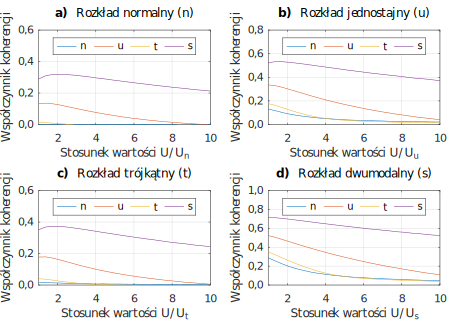
\includegraphics{obrazki/shapes}
\makecaption{fig:unc_shapefac}{Zależność wartości współczynnika koherencji w funkcji stosunku wartości niepewności rozszerzonej dla pary nieskorelowanych sygnałów błędów}
\end{center}
\end{figure}

Drugim analizowanym aspektem jest założenie wynikające z centralnego twierdzenia granicznego, wobec którego wraz ze wzrostem liczby sumowanych sygnałów kształt rozkładu sygnału wypadkowego dążyć będzie do kształtu rozkładu normalnego, jeśli sygnały te nie są skorelowane i nie występuje w nich żaden sygnał dominujący. Korektę wynikającą z opisywanych założeń zaproponowano w pracy~\cite{jakubiec_system} jako:
\begin{equation}
k_{i,j} = k_{j,i} = \frac{U_{i}^{2} + U_{j}^{2}}{\sum _{k = 0} ^{N-1} U_{k}^{2}} \label{eq:unc_cohercorrb},
\end{equation}
co oznacza, że wartość współczynnika koherencji powinna być tym bardziej zbliżona do zera, im więcej istnieje źródeł błędów oraz im bardziej podobne są ich parametry. Należy zauważyć, że wraz ze wzrostem liczby sygnałów błędów cechujących się podobną wartością niepewności rozszerzonej wartość wyrażenia~\eqref{eq:unc_cohercorrb} dążyć będzie do zera tym szybciej, im bardziej zbliżone są wartości niepewności rozszerzonych analizowanych sygnałów.

Biorąc pod uwagę współczynnik kształtu dla pary sygnałów o identycznych wartościach niepewności rozszerzonej opisany równaniem~\eqref{eq:unc_shapertwo}, korektę wynikającą z dysproporcji pomiędzy wartościami niepewności rozszerzonych sumowanych sygnałów opisaną równaniem~\eqref{eq:unc_cohercorra} oraz korektę wynikającą z założeń centralnego twierdzenia daną zależnością~\eqref{eq:unc_cohercorrb}, otrzymuje się zależność umożliwiającą oszacowanie wartości współczynników koherencji dla $N$ nieskorelowanych sygnałów błędów w postaci:
\begin{equation}
h_{i,j} = h_{j,i} = s_{i,j} p_{i,j} k_{i,j} = s_{i,j} \sqrt{\frac{\min \emb{U_{i}, U_{j}}}{\max \emb{U_{i}, U_{j}}}} \left( \frac{U_{i}^{2} + U_{j}^{2}}{\sum _{k = 0} ^{N-1} U_{k}^{2}} \right) \label{eq:unc_coher}.
\end{equation}
Na podstawie przedstawionego równania istnieje możliwość budowy macierzy koherencji, wykorzystywanej do wyznaczenia wypadkowej wartości niepewności rozszerzonej dla analizowanych sygnałów błędów zgodnie z zależnością~\eqref{eq:unc_matrix}.

Należy zauważyć, że z uwagi na możliwość wyznaczenia wartości współczynników kształtu \DIFdelbegin \DIFdel{$s_{i,j}$ }\DIFdelend niezależnie od \DIFdelbegin \DIFdel{parametrów }\DIFdelend \DIFaddbegin \DIFadd{wartości }\DIFaddend niepewności \DIFaddbegin \DIFadd{rozszerzonych }\DIFaddend sygnałów błędów \DIFdelbegin \DIFdel{występujących }\DIFdelend \DIFaddbegin \DIFadd{obecnych }\DIFaddend w analizowanym torze pomiarowym, zaproponowana metoda jest możliwa do stosowania w czasie działania systemu również w przypadkach, gdy parametry \DIFdelbegin \DIFdel{sygnałów }\DIFdelend \DIFaddbegin \DIFadd{te }\DIFaddend ulegają zmianie. Wadą przedstawionego rozwiązania jest konieczność wstępnego wyznaczenia wartości współczynników kształtu dla wszystkich rodzajów rozkładów \DIFaddbegin \DIFadd{realizacji }\DIFaddend sygnałów błędów występujących w analizowanym torze pomiarowym. Dodatkowo\DIFaddbegin \DIFadd{, }\DIFaddend ze względu na uproszczoną formę równania~\eqref{eq:unc_cohercorra}, która nie oddaje w pełni charakteru zależności przedstawionych na rysunku~\ref{fig:unc_shapefac}, wartości oszacowanych współczynników koherencji mogą być obarczone błędem, co w efekcie będzie miało wpływ na pojawienie się błędu oszacowania wartości wypadkowej niepewności rozszerzonej.

Ostatnim wymagającym komentarza jest przypadek, w którym istnieją korelacje pomiędzy analizowanymi sygnałami \DIFaddbegin \DIFadd{błędów}\DIFaddend . Zgodnie z właściwościami macierzy koherencji elementy tej macierzy, podobnie jak elementy macierzy korelacji stosowanej w równaniu~\eqref{eq:var_matrix}, przyjmować mogą wartości z zakresu \DIFdelbegin \DIFdel{$<-1;1>$}\DIFdelend \DIFaddbegin \DIFadd{$\interval{-1}{1}$}\DIFaddend . Dla pełnej dodatniej korelacji wartość współczynnika koherencji wynosić będzie~\num{1}, natomiast dla pełnej ujemnej korelacji wartość ta wyniesie~\num{-1}~\cite{jakubiec_redmono}. W pozostałych przypadkach, zgodnie z informacjami przytoczonymi w poprzedniej części podrozdziału, wartość współczynnika koherencji wynikać będzie z wypadkowych parametrów kształtu splatanych rozkładów oraz współczynnika korelacji. Wobec powyższych nie jest możliwe oszacowanie wartości tego współczynnika stosując metody podobne do zaproponowanych w równaniach od~\eqref{eq:unc_shapertwo} do~\eqref{eq:unc_cohercorrb}. W omawianych sytuacjach, do wyznaczania wartości współczynników koherencji, zastosować należy metodę opisaną w pracy~\cite{jakubiec_reductive}. Inną drogą może być również przeprowadzenie analizy z osobna dla grup skorelowanych sygnałów, a następnie wykorzystanie wyznaczonych parametrów w równaniu~\eqref{eq:unc_matrix}.

Aby zweryfikować zasadność przedstawionych zależności oraz możliwość aplikacji zaproponowanej metody, przeprowadzono eksperyment metodą Monte-Carlo, którego celem było porównanie wartości niepewności rozszerzonej $U_{s}$ uzyskiwanej na drodze eksperymentu, zgodnie z instrukcją~\cite{jcgm_montecarlo}, oraz wartości $U_{c}$ uzyskiwanych zgodnie z równaniem~\eqref{eq:unc_matrix} dla współczynników koherencji wyznaczanych na podstawie równania~\eqref{eq:unc_coher}. Błąd względny $\delta_{U}$ oszacowania wartości niepewności rozszerzonej, wyrażony w procentach, \DIFdelbegin \DIFdel{będzie zatem definiowany }\DIFdelend \DIFaddbegin \DIFadd{zdefiniowano zatem }\DIFaddend w postaci:
\begin{equation}
\delta_{U} = 100 \frac{U_{c} - U_{s}}{U_{s}}~\unit{\percent} \label{eq:unc_error}.
\end{equation}
W ramach eksperymentu generowano $N$ niezależnych sygnałów, których \DIFdelbegin \DIFdel{realizacje }\DIFdelend \DIFaddbegin \DIFadd{kolejne wartości realizacji }\DIFaddend pobierane były z populacji o rozkładach $c_{i}$ i parametrach niepewności rozszerzonej $U_{i}$, \DIFdelbegin \DIFdel{których kolejne realizacje sumowano}\DIFdelend \DIFaddbegin \DIFadd{po czym realizacje te sumowano zgodnie z równaniem}\DIFaddend :
\begin{equation}
e_{\Sigma} \emb{k} = \sum _{i=0} ^{N-1} e_{i} \emb{k} \label{eq:unc_testsignal}.
\end{equation}
Dla \DIFdelbegin \DIFdel{uzyskanego }\DIFdelend \DIFaddbegin \DIFadd{opisanego równaniem~\eqref{eq:unc_testsignal} }\DIFaddend sygnału \DIFaddbegin \DIFadd{$e_{\Sigma}(i)$}\DIFaddend , składającego się ze~\num{100000} próbek, \DIFdelbegin \DIFdel{wyznaczano niepewność rozszerzoną $U_{s}$ }\DIFdelend zgodnie z równaniem~\eqref{eq:unc_summation} \DIFdelbegin \DIFdel{oraz }\DIFdelend \DIFaddbegin \DIFadd{wyznaczano }\DIFaddend wartość \DIFaddbegin \DIFadd{niepewności rozszerzonej $U_{s}$. Wartość niepewności rozszerzonej }\DIFaddend $U_{c}$ \DIFdelbegin \DIFdel{oszacowaną }\DIFdelend \DIFaddbegin \DIFadd{szacowano }\DIFaddend na podstawie równania~\eqref{eq:unc_matrix} \DIFdelbegin \DIFdel{w celu wyznaczenia }\DIFdelend \DIFaddbegin \DIFadd{dla wylosowanych parametrów bieżącej iteracji eksperymentu. Dla uzyskanych wartości omawianych wielkości wyznaczano, }\DIFaddend zgodnie z równaniem~\eqref{eq:unc_error}\DIFaddbegin \DIFadd{, wartość }\DIFaddend względnego błędu oszacowania wartości \DIFdelbegin \DIFdel{analizowanej }\DIFdelend wielkości \DIFaddbegin \DIFadd{$U_{c}$}\DIFaddend . Opisywany proces powtarzano~\num{100000} razy, przy czym wartość $N$ pobierana była dla każdej iteracji z populacji danej przedziałem \DIFdelbegin \DIFdel{$<3,9>$ }\DIFdelend \DIFaddbegin \DIFadd{$\interval{3}{9}$ }\DIFaddend o jednakowym prawdopodobieństwie uzyskania każdej z wartości\DIFdelbegin \DIFdel{. Populacje }\DIFdelend \DIFaddbegin \DIFadd{, populacje }\DIFaddend kolejnych sygnałów \DIFdelbegin \DIFdel{$e_{i}$ }\DIFdelend \DIFaddbegin \DIFadd{$e_{i}(k)$ }\DIFaddend stanowiły losowo kombinację rozkładów: normalnego, jednostajnego, trójkątnego oraz dwumodalnego, \DIFaddbegin \DIFadd{przy czym wylosowanie każdego z rodzajów rozkładu było jednakowo prawdopodobne, }\DIFaddend natomiast wartości \DIFdelbegin \DIFdel{niepewności rozszerzonej }\DIFdelend \DIFaddbegin \DIFadd{parametrów }\DIFaddend $U_{i}$ losowane były z przedziału \DIFdelbegin \DIFdel{$<U_{min};U_{max}>$ }\DIFdelend \DIFaddbegin \DIFadd{$\interval{U_{min}}{U_{max}}$ }\DIFaddend o jednakowym prawdopodobieństwie uzyskania każdej z wartości. \DIFdelbegin \DIFdel{Aby zweryfikować, w jakim stopniu zaproponowany }\DIFdelend \DIFaddbegin \DIFadd{W celu weryfikacji wpływu stosowania zaproponowanego }\DIFaddend w równaniu~\eqref{eq:unc_cohercorra} \DIFdelbegin \DIFdel{współczynnik korekty wpłynął }\DIFdelend \DIFaddbegin \DIFadd{współczynnika korekty }\DIFaddend na skuteczność opisanej w równaniu~\eqref{eq:unc_matrix} metody, \DIFdelbegin \DIFdel{eksperyment przeprowadzono dwukrotnie: stosując wartości współczynników koherencji wyznaczanych zgodnie z równaniem~\eqref{eq:unc_cohercorra} oraz po raz drugi, przyjmując }\DIFdelend wartość \DIFaddbegin \DIFadd{wielkości $\delta_{U}$ obliczano dwukrotnie, przy czym za drugim razem przyjmowano w równaniu~\eqref{eq:unc_coher} założenie }\DIFaddend $p_{i,j} = 1$ dla dowolnej kombinacji $i$ oraz $j$.
\DIFdelbegin \DIFdel{Na podstawie uzyskiwanych realizacji sygnału błędu $e_{\Sigma}(k)$ opisanego równaniem~\eqref{eq:unc_error} sporządzano histogram, który stosowano do oszacowania wartości niepewność rozszerzonej $U_{s}$.
}\DIFdelend 

Ze względu na dużą zmienność parametrów związanych z sumowanymi sygnałami\DIFaddbegin \DIFadd{, }\DIFaddend zaproponowany eksperyment powinien w sposób miarodajny określić typową rozbieżność pomiędzy rzeczywistą, a oszacowaną \DIFdelbegin \DIFdel{za pomocą omawianej metody }\DIFdelend \DIFaddbegin \DIFadd{zgodnie z równaniem~\eqref{eq:unc_matrix} }\DIFaddend wartością niepewności rozszerzonej. \DIFdelbegin \DIFdel{Rysunek~\ref{fig:hist_reductive} przedstawia }\DIFdelend \DIFaddbegin \DIFadd{Na rysunku~\ref{fig:hist_reductive} przedstawiono }\DIFaddend uzyskane histogramy względnego błędu oszacowania wypadkowej wartości niepewności rozszerzonej $\delta_{U}$, natomiast w tabeli~\ref{tab:comp_reductive} \DIFdelbegin \DIFdel{przedstawiono }\DIFdelend \DIFaddbegin \DIFadd{zestawiono }\DIFaddend porównanie uzyskanych wartości niepewności rozszerzonej błędu oszacowania wartości wypadkowej niepewności rozszerzonej $\delta_{U}$ w zależności od stosowania korekty zaproponowanej w równaniu~\eqref{eq:unc_cohercorra}, \DIFdelbegin \DIFdel{wyznaczone }\DIFdelend \DIFaddbegin \DIFadd{które wyznaczono }\DIFaddend zgodnie z~\cite{jcgm_guide, jcgm_montecarlo}. \DIFdelbegin \DIFdel{Analizując wyniki przeprowadzonego eksperymentu zauważyć }\DIFdelend \DIFaddbegin \DIFadd{Na podstawie przedstawionych wyników wnioskować }\DIFaddend można, że \DIFdelbegin \DIFdel{wprowadzenie proponowanej korekty powoduje zmniejszenie szacowanej }\DIFdelend \DIFaddbegin \DIFadd{stosowanie zaproponowanej korekty skutkuje zmniejszeniem wartości względnego błędu oszacowania wypadkowej }\DIFaddend wartości niepewności rozszerzonej \DIFdelbegin \DIFdel{, a także zmniejszenie rozrzutu względnego }\DIFdelend \DIFaddbegin \DIFadd{oraz zmniejszeniem rozrzutu tego }\DIFaddend błędu\DIFdelbegin \DIFdel{oszacowania tej wielkości}\DIFdelend . W efekcie\DIFaddbegin \DIFadd{, stosując omawianą korektę, }\DIFaddend możliwe jest oszacowanie wartości wypadkowej niepewności rozszerzonej z błędem względnym mieszczącym się w przedziale~\qty{\pm 5}{\percent}.

\DIFdelbegin %DIFDELCMD < \begin{table}[htb!]
%DIFDELCMD < \begin{center}
%DIFDELCMD < \makecaption{tab:comp_reductive}{Zestawienie wartości niepewności względnego błędu szacowania wypadkowej wartości niepewności rozszerzonej w zależności od stosowania zaproponowanej w pracy korekty współczynnika kształtu uzyskane metodą Monte-Carlo dla poziomu ufności~\qty{95}{\percent}}
%DIFDELCMD < \begin{tabular}[c]{| c *{8}{|S[table-format = +1.2]} |} \hline
%DIFDELCMD < \textbf{$U_{i}$} & \multicolumn{2}{c|}{\textbf{a) $<1;3>$}} & \multicolumn{2}{c|}{\textbf{b) $<1;6>$}} & \multicolumn{2}{c|}{\textbf{c) $<1;10>$}} & \multicolumn{2}{c|}{\textbf{d) $<1;20>$}} \\ \hline
%DIFDELCMD < \textbf{$\delta_{U}$} & \textbf{$U_{-}$} & \textbf{$U_{+}$} & \textbf{$U_{-}$} & \textbf{$U_{+}$} & \textbf{$U_{-}$} & \textbf{$U_{+}$} & \textbf{$U_{-}$} & \textbf{$U_{+}$} \\ \hline
%DIFDELCMD < Z korektą   & -2.23 & +4.83 & -2.43 & +4.59 & -2.54 & +4.52 & -2.62 & +4.45 \\ \hline
%DIFDELCMD < Bez korekty & -1.14 & +7.96 & -1.13 & +8.69 & -1.09 & +8.80 & -1.13 & +8.86 \\ \hline
%DIFDELCMD < \end{tabular}
%DIFDELCMD < \end{center}
%DIFDELCMD < \end{table}
%DIFDELCMD < %%%
\DIFdelend \DIFaddbegin \begin{table}[htb!]
\begin{center}
\makecaption{tab:comp_reductive}{Zestawienie wartości niepewności względnego błędu szacowania wypadkowej wartości niepewności rozszerzonej w zależności od stosowania zaproponowanej w pracy korekty współczynnika kształtu uzyskane metodą Monte-Carlo dla poziomu ufności~\qty{95}{\percent}}
\begin{tabular}[c]{| c *{8}{|S[table-format = +1.2]} |} \hline
\textbf{$U_{i}$} & \multicolumn{2}{c|}{\textbf{a) $\interval{1}{3}$}} & \multicolumn{2}{c|}{\textbf{b) $\interval{1}{6}$}} & \multicolumn{2}{c|}{\textbf{c) $\interval{1}{10}$}} & \multicolumn{2}{c|}{\textbf{d) $\interval{1}{20}$}} \\ \hline
\textbf{$\delta_{U}$} & \textbf{$U_{-}$} & \textbf{$U_{+}$} & \textbf{$U_{-}$} & \textbf{$U_{+}$} & \textbf{$U_{-}$} & \textbf{$U_{+}$} & \textbf{$U_{-}$} & \textbf{$U_{+}$} \\ \hline
Z korektą   & -2.23 & +4.83 & -2.43 & +4.59 & -2.54 & +4.52 & -2.62 & +4.45 \\ \hline
Bez korekty & -1.14 & +7.96 & -1.13 & +8.69 & -1.09 & +8.80 & -1.13 & +8.86 \\ \hline
\end{tabular}
\end{center}
\end{table}
\DIFaddend 

\begin{figure}[htb!]
\begin{center}
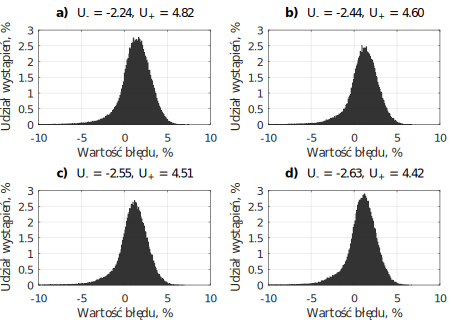
\includegraphics{obrazki/hist_reductive}
\makecaption{fig:hist_reductive}{Histogramy względnego błędu oszacowania wypadkowej wartości niepewności rozszerzonej dla zaproponowanej w pracy metody odpowiadające danym zestawionym w tabeli~\ref{tab:comp_reductive}}
\end{center}
\end{figure}

Analizując przedstawione dotychczas zależności zauważyć można, że sposób opisu niedokładności wyniku pomiaru zależeć będzie w dużej mierze od potrzeb projektanta toru pomiarowego oraz od specyfiki zakłócających proces pomiaru zjawisk. Opis wykorzystujący wariancję sygnału błędu wydaje się bardziej przystępny i mniej skomplikowany, a dodatkowo wielkość ta może być utożsamiana z mocą sygnału~\cite{proakis_dsp}. Opis wykorzystujący niepewność rozszerzoną będzie jednak bardziej precyzyjny, ze względu na informacje odnośnie prawdopodobieństwa wystąpienia danej wartości realizacji sygnału błędu, natomiast wymaga on większego zaangażowania w proces wyznaczania ostatecznej wartości tej wielkości. W odpowiednich okolicznościach, jeżeli spełnione są warunki związane z centralnym twierdzeniem granicznym, opis bazujący na wariancji sygnału błędu może być w łatwy sposób przeniesiony na opis związany z niepewnością rozszerzoną~\cite{jcgm_guide}.

Wyznaczone zgodnie z metodą redukcyjnej arytmetyki interwałowej szacowane wartości niepewności rozszerzonej mogą w niewielkim stopniu odbiegać od wartości rzeczywistych, co opisano w~\cite{jakubiec_redmono, jakubiec_model}. Zaproponowana w równaniu~\eqref{eq:unc_cohercorra} korekta zmniejsza omawiane różnice, zapewniając jednocześnie niski stopnień skomplikowania obliczeń oraz względny błąd oszacowania wypadkowej wartości niepewności rozszerzonej nieprzekraczający~\qty{\pm 5}{\percent} prawidłowej wartości tej wielkości. Można zatem stwierdzić, że zaproponowana w pracy metoda szacowania wypadkowej wartości niepewności rozszerzonej jest zasadna z punktu widzenia przyjętych założeń. Ponadto, ze względu na niską złożoność obliczeń, metoda ta może być stosowana w przypadkach, gdzie liczba analizowanych sygnałów oraz ich parametry ulegają zmianie\DIFaddbegin \DIFadd{~\mbox{%DIFAUXCMD
\cite{auth_reductive}}\hskip0pt%DIFAUXCMD
}\DIFaddend .

\section{Algorytm jako fragment toru pomiarowego}

Podczas opisu właściwości cyfrowej części toru pomiarowego przedstawiono przypadek ogólny, w którym analizowany obiekt przetwarzał kolejne próbki sygnału wejściowego na próbki sygnału wyjściowego zgodnie z odpowiadającą mu transmitancją i funkcją przetwarzania. Algorytmy stosowane w torach pomiarowych mogą generować wiele wielkości wyjściowych, pobierając w tym celu określoną liczbę próbek wielkości wejściowych. W przypadku, gdy wyjście analizowanego obiektu stanowi $M$ próbek wielkości wyjściowych wyznaczanych na podstawie $N$ próbek wielkości wejściowych, a funkcja przetwarzania oraz transmitancja tego obiektu są liniowe i niezmienne w czasie, działanie obiektu przedstawić można w postaci równania~\cite{jakubiec_algorithms, jakubiec_single}:
\begin{equation}
\begin{bmatrix}
X \emb{0}   \\
X \emb{1}   \\
\vdots      \\
X \emb{M-1}
\end{bmatrix}
=
\begin{bmatrix}
a_{0, 0}   &   a_{0, 1} &   \cdots   &   a_{0, N-1}      \\
a_{1, 0}   &   \ddots   &            &   a_{1, N-1}      \\
\vdots     &            &   \ddots   &   \vdots          \\
a_{M-1, 0} &   \cdots   &   \cdots   &   a_{M-1, N-1}
\end{bmatrix}
\begin{bmatrix}
x \emb{0}   \\
x \emb{1}   \\
\vdots      \\
x \emb{N-1}
\end{bmatrix}
\label{eq:alg_out_mat},
\end{equation}
gdzie $a_{i,j}$ to kolejne współczynniki macierzy transformacji, $X(i)$ to kolejne wielkości \DIFdelbegin \DIFdel{wejściowe}\DIFdelend \DIFaddbegin \DIFadd{wyjściowe}\DIFaddend , natomiast $x(j)$ to kolejne wielkości wejściowe analizowanego algorytmu. Równanie~\eqref{eq:alg_out_mat} można przedstawić również w postaci iloczynu~\cite{jakubiec_algorithms}:
\begin{equation}
\mathbf{X} = \mathbf{A} \cdot \mathbf{x} \label{eq:alg_out_mul},
\end{equation}
gdzie $\mathbf{X}$ jest wektorem wielkości wyjściowych, $\mathbf{A}$ macierzą transformacji oraz $\mathbf{x}$ wektorem wielkości wejściowych. Wobec powyższych zależności, pojedynczą wielkość wyjściową algorytmu przedstawić można w postaci:
\begin{equation}
X \emb{i} = a_{i, 0} x \emb{0} + a_{i, 1} x \emb{1} + \hdots + a_{i, N-1} x \emb{N-1} = \sum _{j = 0} ^{N-1} a_{i,j} x \emb{j} \label{eq:alg_out_single}.
\end{equation}
Na podstawie równania~\eqref{eq:alg_out_single} zauważyć można, że analizowany obiekt stanowi zbiór filtrów o skończonej odpowiedzi impulsowej \enquote{FIR} (ang. \enquote{Finite Impulse Response}). Przedstawione metody analizy będą zatem przypominały metody analizy opisywanego typu filtru~\cite{mehrnia_fir}. Przedstawione założenie odnośnie stałej transmitancji algorytmu implikuje niezmienność wartości elementów macierzy transformacji analizowanego algorytmu. W przypadku, gdy istnieje konieczność analizy algorytmu o zmiennej transmitancji, przy zmianie tej transmitancji należy każdorazowo wyznaczyć wartości wszystkich wielkości od niej zależnych.

Jako, że w procesie przetwarzania danych stosuje \DIFaddbegin \DIFadd{się }\DIFaddend zwykle gotowe algorytmy, zaimplementowane np. w środowiskach \enquote{GNU Octave} czy \enquote{Matlab}~\cite{pruuvsa_dwt, lee_pywavelets}, wartości współczynników macierzy transformacji $\mathbf{A}$ stosowanej w równaniach~\eqref{eq:alg_out_mat} oraz~\eqref{eq:alg_out_mul} mogą nie być znane. Jeżeli znana jest transmitancja $H_{i}(z)$ dla kolejnych wielkości wyjściowych, wyznaczenie wartości współczynników macierzy transformacji odbywać się będzie poprzez przekształcenie tej transmitancji na postać zgodną z równaniem~\eqref{eq:alg_out_single}, przy czym zabieg ten nie jest konieczny. Analiza właściwości metrologicznych w omawianym przypadku przebiegać może identycznie, jak miało to miejsce w przypadku cyfrowego fragmentu toru pomiarowego, natomiast wyznaczenie wartości współczynników macierzy transformacji przy znajomości transmitancji algorytmu pozwoli w pewnym stopniu uprościć analizę, co przedstawiono w dalszej części podrozdziału. \DIFdelbegin \DIFdel{Drugim }\DIFdelend \DIFaddbegin \DIFadd{Innym }\DIFaddend przypadkiem jest sytuacja, \DIFdelbegin \DIFdel{w której }\DIFdelend \DIFaddbegin \DIFadd{gdzie }\DIFaddend wartości współczynników \DIFaddbegin \DIFadd{macierzy transformacji }\DIFaddend mogą być wyznaczone analitycznie\DIFaddbegin \DIFadd{, }\DIFaddend za pomocą odpowiednich zależności opisujących stosowany algorytm, jak ma to zwykle miejsce w przypadku algorytmów dyskretnej transformacji falkowej~\cite{vonesch_dbbasics}. Ostatnim analizowanym w pracy przypadkiem jest sytuacja, w której dostępna jest implementacja stosowanego algorytmu, natomiast nie jest znana jego struktura numeryczna~\cite{misiti_matlabwav}.

Jeżeli analizowany algorytm jest liniowy oraz jego transmitancja jest liniowa i niezmienna w czasie, związek pomiędzy transmitancją $H_{i}(z)$ dla $i$-tej wielkości wyjściowej oraz $i$-tym wierszem macierzy transformacji $\mathbf{A}$ może być opisany równaniem:
\begin{equation}
H_{i} \emb{z} = a_{i, 0} + a_{i, 1} z^{-1} + \hdots + a_{i, N-1} z^{-N+1} = \sum _{k = 0} ^{N-1} a_{i, k} z^{-k} \label{eq:alg_trans_single}.
\end{equation}
Przedstawiona zależność umożliwia wyznaczenie wartości współczynników macierzy transformacji przy znajomości transmitancji wielkości wyjściowych algorytmu oraz wyznaczenie transmitancji tych wielkości przy znajomości wartości macierzy transformacji tego algorytmu. W celu wyznaczenia transmitancji $H_{i}(z)$ dla $i$-tej wielkości wyjściowej algorytmu w dziedzinie pulsacji, odpowiedniej dla okresu próbkowania $T_{p}$, należy przyjąć w równaniu~\eqref{eq:alg_trans_single} założenie, że $z = e^{j\omega T_{p}}$~\cite{proakis_dsp}.

Identyfikacja wartości współczynników macierzy transformacji w przypadku istniejącego algorytmu polega na wyznaczaniu odpowiedzi tego algorytmu dla wektora wielkości wejściowych o wartościach zgodnych z równaniem~\cite{jakubiec_algorithms, jakubiec_system}:
\begin{equation}
x \emb{n} =
\begin{cases}
	1 & $gdy$~n = j \\
	0 & $gdy$~n \neq j
\end{cases}
\label{eq:wt_ident},
\end{equation}
przy czym uzyskany wektor wielkości wyjściowych stanowi $j$-tą kolumnę macierzy transformacji tego algorytmu. Przedstawioną operację należy wykonać dla wszystkich kolumn macierzy transformacji, a zatem dla $j$ w przedziale \DIFdelbegin \DIFdel{$<0;N-1>$}\DIFdelend \DIFaddbegin \DIFadd{$\interval{0}{N-1}$}\DIFaddend . Opisana metoda jest uniwersalna, przy czym wymaga ona, aby identyfikowany algorytm spełniał założenia przedstawione na początku podrozdziału.

Przedstawione dotychczas zależności podkreślają ścisły związek pomiędzy transmitancją kolejnych wielkości wyjściowych algorytmu oraz wartościami macierzy transformacji. Należy zauważyć, że z punktu widzenia zaproponowanego w pracy modelu, rozpatrywany algorytm mógłby być analizowany jako kilka obiektów cyfrowej części toru pomiarowego, przetwarzających te same wielkości wejściowe $x(i)$ na odpowiednie wielkości wyjściowe $X_{j}(i)$. Przedstawienie algorytmu w postaci macierzowej pozwala natomiast ujednolicić analizę i sprowadzić ją do zastąpienia opisywanej grupy obiektów jednym obiektem. Mnogość sposobów wyznaczania wartości elementów macierzy transformacji stanowi dodatkowy, cenny walor proponowanej metody analizy.

Aby ustalić związek pomiędzy sygnałami błędów wielkości wejściowych, a sygnałami błędów wielkości wyjściowych analizowanego algorytmu, należy rozważyć proces wyznaczania wartości pojedynczej wielkości wyjściowej tego obiektu. Zakładając, że wielkości wejściowe algorytmu są obarczone realizacjami sygnałów błędów o charakterze addytywnym zgodnie z zależnością:
\begin{equation}
\tilde{x} \emb{i} = \dot{x} \emb{i} + e_{x,s} \emb{i} + e_{x,d} \emb{i} + e_{x,r} \emb{i} = \dot{x} \emb{i} + e_{x,\Sigma} \emb{i} \label{eq:alg_inputval},
\end{equation}
gdzie $e_{x,s}(i)$ oznacza błąd statyczny, $e_{x,d}(i)$ błąd dynamiczny oraz $e_{x,r}(i)$ błąd losowy wielkości wejściowej, istnieje możliwość osobnej analizy wyniku realizacji algorytmu dla idealnych wartości wielkości wejściowych oraz dla wymienionych sygnałów błędów. Sygnał błędu $e_{X,p}(i)$ propagowanego z wejścia na wyjście analizowanego algorytmu można zatem opisać zgodnie z równaniem~\eqref{eq:alg_out_single} w postaci:
\begin{equation}
e_{X,p} \emb{i} = a_{i, 0} e_{x,\Sigma} \emb{0} + a_{i, 1} e_{x,\Sigma} \emb{1} + \hdots + a_{i, N-1} e_{x,\Sigma} \emb{N-1} = \sum _{j = 0} ^{N-1} a_{i,j} e_{x,\Sigma} \emb{j} \label{eq:alg_outerr}.
\end{equation}
Realizacja propagowanego sygnału błędu $e_{X,p}(i)$ stanowi zatem kombinację liniową współczynników $i$-tego wiersza macierzy transformacji oraz wektora realizacji sygnału błędu wielkości wejściowych algorytmu.

Dla sygnałów błędów o charakterze statycznym, ze względu na fakt że wartość realizacji tych sygnałów jest niezmienna w obrębie pojedynczego okna pomiarowego, równanie~\eqref{eq:alg_outerr} można uprościć i zapisać w postaci:
\begin{equation}
e_{X,sp} \emb{i} = a_{i, 0} e_{x,s} \emb{k} + a_{i, 1} e_{x,s} \emb{k} + \hdots + a_{i, N-1} e_{x,s} \emb{k} = e_{x,s} \emb{k} \sum _{j = 0} ^{N-1} a_{i, j} \label{eq:alg_outerr_stat},
\end{equation}
gdzie $e_{x,s}(k)$ jest błędem statycznym wielkości wejściowej dla $k$-tego okna pomiarowego, natomiast $e_{X,sp}(i)$ błędem statycznym propagowanym wielkości wyjściowej algorytmu. Powtarzając proces wyznaczania wartości wielkości wyjściowej algorytmu wielokrotnie, dla różnych numerów okna pomiarowego realizacje sygnału błędu statycznego mogą przyjmować różne wartości. W takim przypadku wyjściowy błąd statyczny również można rozpatrywać w kategoriach probabilistycznych, a jego wariancję opisać można równaniem uwzględniającym wariancję sygnału wejściowego błędu statycznego:
\begin{equation}
\sigma_{X,sp}^{2} \emb{i} = \sigma_{x,s}^{2} \left( a_{i, 0} + a_{i, 1} + \hdots + a_{i, N-1} \right)^{2} = \sigma_{x,s}^{2} \left( \sum _{j = 0} ^{N-1} a_{i, j} \right)^{2} \label{eq:alg_outvar_stat}.
\end{equation}
Należy zauważyć, że kształt rozkładu sygnału wyjściowego błędu statycznego będzie identyczny, jak kształt rozkładu sygnału błędu statycznego na wejściu algorytmu.

Dla sygnałów błędów dynamicznych należy przeprowadzić analizę zgodnie z metodologią przedstawioną w poprzedniej części rozdziału, wykorzystując znajomość transmitancji $H_{i}(z)$ odpowiedniej dla analizowanej wielkości wyjściowej algorytmu. Identycznie, jak w przypadku równania~\eqref{eq:mid_disc_err_dyn_prop}, wyznaczyć należy wypadkowe amplitudy oraz przesunięcia w fazie kolejnych harmonicznych sygnału propagowanego błędu dynamicznego, a następnie wykorzystać należy równania od~\eqref{eq:dyn_harm} do~\eqref{eq:dyn_corr} w celu wyznaczenia wariancji analizowanych sygnałów. Na podstawie wskazanych zależności, wariancję $\sigma_{X,dp}^{2}(\omega)$ pojedynczej harmonicznej sygnału propagowanego błędu dynamicznego $e_{x,d}(i)$ wyznaczyć można zgodnie z zależnością:
\begin{equation}
\sigma_{X,dp}^{2} \emb{i, \omega} = \frac{1}{2} E_{x,e}^{2} \emb{\omega} \left| H_{i} \emb{e^{j\omega T_{p}}} \right|^{2} \label{eq:alg_outvar_dyn},
\end{equation}
gdzie $E_{x,e}(\omega)$ jest amplitudą analizowanej harmonicznej sygnału błędu dynamicznego $e_{x,d}(i)$ o pulsacji $\omega$, natomiast $T_{p}$ okresem próbkowania wielkości wejściowych algorytmu.

Sygnały błędów niedeterministycznych propagowane są przez analizowany algorytm w sposób identyczny, jak miało to miejsce w przypadku cyfrowej części toru pomiarowego. W ogólnym przypadku można zatem wykorzystać zależność~\eqref{eq:mid_disc_var_omega} w celu określenia wariancji $\sigma_{X,rp}^{2}(\omega)$ propagowanego sygnału błędu losowego $e_{x,r}(i)$ w funkcji pulsacji. Wyznaczenie średniej wartości omawianej wielkości może odbywać się zgodnie z równaniem~\eqref{eq:mid_disc_var_rand}, przy czym należy wyznaczać ją dla wartości pulsacji zawartych w przedziale \DIFdelbegin \DIFdel{$<0; \frac{1}{2} \omega_{p}>$}\DIFdelend \DIFaddbegin \DIFadd{$\interval{0}{\frac{1}{2} \omega_{p}}$}\DIFaddend . Jeżeli analizowany sygnał błędu losowego $e_{x,r}(i)$ cechuje się stałą widmową gęstością mocy, to obliczenia można uprościć stosując do wyznaczenia wartości wariancji losowego sygnału błędu na wyjściu algorytmu zależność~\cite{jakubiec_system}:
\begin{equation}
\sigma_{rp}^{2} \emb{i} = a_{i, 0}^{2} \sigma_{x,r}^{2} + a_{i, 1}^{2} \sigma_{x,r}^{2} + \hdots + a_{i, N-1}^{2} \sigma_{x,r}^{2} = \sigma_{x,r}^{2} \sum _{j=0} ^{N-1} {a_{i, j}^{2}} \label{eq:alg_outvar_rand}.
\end{equation}
Równania~\eqref{eq:mid_disc_var_rand} oraz~\eqref{eq:alg_outvar_rand} są zatem równoważne dla przypadków gdzie $\sigma_{x,r}^{2}(\omega) = \text{const}$.

Znajomość wartości kolejnych elementów macierzy transformacji pozwala na podstawie równań~\eqref{eq:alg_outvar_stat} oraz~\eqref{eq:alg_outvar_rand} wprowadzić dodatkowe wielkości, opisane następującymi zależnościami~\cite{jakubiec_algorithms, oppenheim_dsp, proakis_dsp}:
\begin{gather}
A_{i,s} = \sum _{j = 0} ^{N-1} a_{i, j} = \left| H_{i} \emb{1} \right| \label{eq:alg_trans_stat}, \\
A_{i,r} = \sqrt{\sum _{j = 0} ^{N-1} a_{i, j}^{2}} = \sqrt{\frac{1}{\pi} \int _{0} ^{\pi} \left| H_{i} \emb{e^{j \omega}} \right|^{2} d\omega} \label{eq:alg_trans_rand},
\end{gather}
gdzie $A_{i,s}$ jest współczynnikiem przenoszenia \DIFdelbegin \DIFdel{dla }\DIFdelend \DIFaddbegin \DIFadd{sygnałów }\DIFaddend błędów statycznych, natomiast \DIFdelbegin \DIFdel{jest }\DIFdelend $A_{i,r}$ \DIFaddbegin \DIFadd{jest }\DIFaddend współczynnikiem przenoszenia \DIFdelbegin \DIFdel{dla }\DIFdelend \DIFaddbegin \DIFadd{sygnałów }\DIFaddend błędów losowych \DIFaddbegin \DIFadd{dla }\DIFaddend $i$-tej wielkości wyjściowej analizowanego algorytmu. Wyznaczenie wartości opisanych współczynników umożliwi wyznaczenie wariancji kolejnych sygnałów błędów losowych oraz statycznych, a dodatkowo będzie stanowiło informacje, w jaki sposób analizowany algorytm przenosi z wejścia na wyjście określony rodzaj błędów. Można zauważyć, że dla niskich wartości współczynnika przenoszenia (tj. $A_{i} < 1$) kolejne błędy wielkości wejściowych będą tłumione (wariancja sygnału błędu wielkości wyjściowej będzie mniejsza, niż wariancja sygnału błędu wielkości wejściowej). Odwrotna sytuacja będzie miała miejsce w przypadku dużych wartości współczynnika (tj. $A_{i} > 1$). Wobec powyższych zachodzi:
\begin{gather}
\sigma_{X,sp}^{2} = \sigma_{x,s}^{2} A_{i,s}^{2} \label{eq:alg_outvar_trans_stat}, \\
\sigma_{X,rp}^{2} = \sigma_{x,r}^{2} A_{i,r}^{2} \label{eq:alg_outvar_trans_rand}.
\end{gather}
Należy zauważyć, że stosowanie równania~\eqref{eq:alg_outvar_trans_rand} pozwala oszacować średnią widmową gęstość mocy analizowanego sygnału błędu tylko w przypadku, gdy sygnał ten cechuje się stałą widmową gęstością mocy. Wyznaczenie średniej wariancji sygnału błędu losowego będzie zasadne dla przypadków, gdzie dalsza analiza wpływu kolejnych obiektów na rozważany sygnał błędu nie będzie prowadzona, zatem gdy obiekt stanowi ostatnią część toru pomiarowego. W innym wypadku należy zastosować zależność~\eqref{eq:mid_disc_var_omega}.

Poza przenoszeniem przez algorytm błędów zawartych w wielkościach wejściowych na jego wyjście, algorytm wprowadza do wielkości wyjściowych błędy własne. W pracy przyjmuje się, że transmitancja algorytmu jest idealna, a zatem algorytm ten nie wprowadza do sygnału wyjściowego błędów własnych o charakterze deterministycznym. Wobec przedstawionego założenia, błędy własne algorytmu wynikają z niedokładności wyznaczenia współczynników algorytmu oraz z przeprowadzanych podczas obliczeń zaokrągleń. Analiza właściwości sygnałów błędów związanych z omawianymi zjawiskami powinna zatem odbywać się indywidualnie dla zaimplementowanego algorytmu.

Zakładając, że wyznaczanie wartości realizacji $i$-tej wielkości wyjściowej algorytmu odbywać się będzie wielokrotnie, sygnały błędów własnych algorytmu opisywać można w kategorii probabilistycznej za pomocą związanej z nimi wariancji $\sigma_{X,rw}^{2}(i)$. Ze względu na fakt, że liczba operacji mnożenia i dodawania, odpowiedzialnych za powstawanie omawianej grupy błędów będzie duża ($N$ mnożeń oraz $N$ dodawań) zakładać można, że błąd ten będzie miał rozkład zbliżony do normalnego~\cite{jcgm_guide}. Należy jednak przeprowadzić odpowiedni eksperyment mający na celu identyfikacje opisywanych zależności, co przedstawiono na przykładzie w dalszej cześć pracy.

W przypadku, gdy na etapie identyfikacji wartości macierzy współczynników uzyskano wartości obarczone błędami, należy rozszerzyć analizę o przedstawienie konsekwencji tego zjawiska. W takim przypadku należy przeanalizować wprowadzany do wielkości wyjściowych dodatkowy błąd własny oraz wykonać analizę dla błędów własnych dynamicznych zgodnie z równaniem~\eqref{eq:mid_disc_err_dyn_self}. Identyczne kroki należy podjąć, jeżeli rzeczywista transmitancja algorytmu różni się od transmitancji wymaganej z punktu widzenia jego działania. Przedstawiony przypadek nie został rozważony w pracy, natomiast omawianą analizę przedstawia monografia~\cite{jakubiec_system}.

Zgodnie z zależnością~\eqref{eq:alg_out_single} $i$-tą wielkość wyjściową $X(i)$ analizowanego algorytmu w przypadku idealnym opisać można następującym równaniem:
\begin{equation}
\dot{X} \emb{i} = \sum _{j = 0} ^{N-1} \dot{a}_{i,j} \dot{x} \emb{j} \label{eq:alg_out_ideal},
\end{equation}
natomiast gdy rozważana wielkość jest zakłócona sygnałem błędu $e_{X,\Sigma}(i)$ zapisać można:
\begin{gather}
\tilde{X} \emb{i} = \dot{X} \emb{i} + e_{X,\Sigma} \emb{i} \label{eq:alg_out_real}, \\
e_{X,\Sigma} \emb{i} = e_{X,w} \emb{i} + e_{X,p} \emb{i} \label{eq:alg_out_err},
\end{gather}
gdzie sygnały błędów własnego $e_{X,w}(i)$ oraz propagowanego $e_{X,p}(i)$ przedstawić można w postaci sumy składowych tych sygnałów, przy czym:
\begin{gather}
e_{X,w} \emb{i} = e_{X,sw} \emb{i} + e_{X,dw} \emb{i} + e_{X,rw} \emb{i} \label{eq:alg_out_err_self}, \\
e_{X,p} \emb{i} = e_{X,sp} \emb{i} + e_{X,dp} \emb{i} + e_{X,rp} \emb{i} \label{eq:alg_out_err_prop}.
\end{gather}
Rozważając podział sygnałów błędów ze względu na charakter ich realizacji, równania~\eqref{eq:alg_out_err_self} oraz~\eqref{eq:alg_out_err_prop} zapisać można również w postaci:
\begin{gather}
e_{X,s} \emb{i} = e_{X,sw} \emb{i} + e_{X,sp} \emb{i} \label{eq:alg_out_err_stat}, \\
e_{X,d} \emb{i} = e_{X,dw} \emb{i} + e_{X,dp} \emb{i} \label{eq:alg_out_err_dyn}, \\
e_{X,r} \emb{i} = e_{X,rw} \emb{i} + e_{X,rp} \emb{i} \label{eq:alg_out_err_rand}.
\end{gather}

Dokładna postać wymienionych w równaniach od~\eqref{eq:alg_out_err_self} do~\eqref{eq:alg_out_err_rand} sygnałów błędów zależeć będzie od właściwości analizowanego algorytmu. Należy zatem wykorzystać przedstawione w bieżącym rozdziale zależności w celu określenia wzajemnych relacji pomiędzy sygnałami błędów na wejściu i wyjściu algorytmu oraz zdefiniować istotne z punktu widzenia właściwości metrologicznej sygnały błędów własnych analizowanego algorytmu. Przykład aplikacji omawianej metody przedstawiono w dalszej części pracy.

Wobec powyższych, w celu wyznaczenia wariancji $\sigma_{X,\Sigma}^{2}(i)$ wypadkowego sygnału błędu $e_{X,\Sigma}(i)$ dla $i$-tej wielkości wyjściowej analizowanego algorytmu należy wykorzystać zależność~\eqref{eq:var_matrix}. Wyznaczenie niepewności rozszerzonej w przypadku omawianego sygnału może być natomiast przeprowadzone zgodnie z zależnością~\eqref{eq:unc_matrix}. W przedstawionych \DIFdelbegin \DIFdel{równaniu }\DIFdelend \DIFaddbegin \DIFadd{równaniach }\DIFaddend uwzględnić należy parametry wszystkich zidentyfikowanych sygnałów błędów, obecnych w sygnale związanym z analizowaną wielkością wyjściową.

Należy zauważyć, że ze względu na właściwości stosowanej w pracy metody szacowania wypadkowej wartości niepewności rozszerzonej, najbardziej korzystnym podejściem jest analiza każdego sygnału błędu z osobna. Omówiona właściwość wynika z zaproponowanego sposobu szacowania wartości współczynników koherencji, opisanego równaniem~\eqref{eq:unc_coher}, wymagającego znajomości wartości współczynników kształtu dla analizowanych par sygnałów. Należy zauważyć, że w wyniku sumowania kolejnych sygnałów błędów i analizy wypadkowego sygnału błędu, sygnał ten może cechować się rozkładem o nietypowym kształcie~\cite{auth_electronics, zhang_pdp}.

\section{Model błędów spowodowanych opóźnieniami}

Przeprowadzone rozważania nie poruszały problemu opóźnień w systemach pomiarowo-sterujących, a zatem nie brano w nich pod uwagę sygnałów błędów związanych z możliwymi opóźnieniami. Mimo, że tematyka pracy nie obejmuje przedstawionego zagadnienia, warto jednak zauważyć, że zaproponowany model błędów może być \DIFdelbegin \DIFdel{z }\DIFdelend dopasowany do możliwości analizy właściwości i wpływu tych zjawisk na niedokładność wyznaczania wartości wielkości wyjściowych rozważanego toru pomiarowego. Należy w takim przypadku uwzględnić w modelu dodatkowy sygnał błędu, który definiować można zgodnie z metodą zaproponowaną w pracach~\cite{wymyslo_delay, jakubiec_system} oraz uwzględnić wpływ analizowanego zjawiska na propagację przez obiekt pozostałych sygnałów błędów.

Z punktu widzenia zaproponowanego modelu błędów, zjawisko opóźnień w systemie opisać można jako dodatkowe przesunięcie w fazie składowych przetwarzanego sygnału oraz sygnałów błędów deterministycznych, będące iloczynem pulsacji analizowanej harmonicznej i wartości realizacji błędu opóźnienia. Omawiany sygnał mógłby być zdefiniowany w przypadku przetwornika analogowo-cygrowego jako dodatkowa harmoniczna sygnału błędu dynamicznego własnego:
\begin{equation}
\begin{split}
e_{x,tw} \emb{i,\omega} =~
& E_{y,o} \emb{\omega} \sin \left( \omega i T_{p} + \varphi_{y,o} \emb{\omega} + \varphi_{x,t} \emb{\omega, i} \right) - \\
& E_{y,o} \emb{\omega} \sin \left( \omega i T_{p} + \varphi_{y,o} \emb{\omega} \right)
\end{split}
\label{eq:tim_err_self},
\end{equation}
gdzie $t_{x}(i)$ stanowi realizację opóźnienia dla $i$-tej wielkości wyjściowej analizowanego obiektu przetwarzającego ciągły w czasie sygnał $y(t)$ na jego dyskretne próbki $x(i)$, natomiast $\varphi_{x,t}(\omega, i)$ jest realizacją przesunięcia fazowego analizowanej harmonicznej dla $i$-tej wielkości wyjściowej i wynosi:
\begin{equation}
\varphi_{x,t} \emb{\omega, i} = \omega t_{x} \emb{i} \label{eq:tim_err_phi}.
\end{equation}
Należy zaznaczyć, że w przypadku analizy opóźnień równania opisujące propagowany przez związany z opóźnieniami obiekt sygnał błędu dynamicznego również musiałyby zostać zmodyfikowane z uwzględnieniem wprowadzanego opóźnienia, jeżeli z punktu widzenia tej analizy istotna byłaby faza tych sygnałów.

Przedstawiona w równaniu~\eqref{eq:tim_err_self} koncepcja stanowi jedynie pojedynczy przypadek analizy opóźnienia w działaniu fragmentu toru pomiarowego. Celem poruszenia przedstawionego zagadnienia, mimo że nie obejmuje ono tematyki pracy, było podkreślenie możliwości dalszego rozwoju zaproponowanego modelu błędów o możliwość analizy kolejnych źródeł niedokładności wyznaczania wartości wielkości wyjściowych torów pomiarowych. Przedstawione zagadnienie może stanowić dalsze prace badawcze, w szczególności że stanowi ono tematykę bardzo istotną z punktu widzenia torów pomiarowych implementujących współbieżnie realizowane zadania pod nadzorem odpowiedniego systemu operacyjnego czasu rzeczywistego~\cite{bandyszak_rtos, laplante_rtos}.

\section{Podsumowanie rozdziału}

W poprzednich częściach rozdziału przedstawiono modele kolejnych fragmentów toru pomiarowego, które opisywały związki pomiędzy sygnałami błędów na wejściu i wyjściu analizowanego obiektu oraz wskazywały rolę tego obiektu we wprowadzaniu do sygnału wyjściowego sygnałów błędów własnych. Zaproponowany model wprowadzał podział na statyczne i dynamiczne właściwości obiektu, które opisywane były transmitancją i funkcją przetwarzania obiektu. Opisane zgodnie z zaproponowanym modelem fragmenty toru pomiarowego, które zostały ze sobą połączone kaskadowo oraz cechują się addytywną i liniową funkcją przetwarzania, opisać można pojedynczym obiektem o wypadkowych właściwościach analizowanych fragmentów.

Przedstawiony model oceny niedokładności wyniku pomiaru zakłada, że obecne w sygnale pomiarowym sygnały błędów cechują się symetrycznymi rozkładami o zerowej wartości oczekiwanej. W przypadku, gdy wartość oczekiwana realizacji sygnału błędu jest niezerowa, błąd ten posiada składową systematyczną, którą należy skorygować w ostatecznym wyniku pomiaru. Jeżeli nie jest spełnione założenie odnośnie symetrii rozkładów składanych błędów, to do określenia rozkładu błędu wynikowego należy stosować metodę analityczną bazującą na wyznaczeniu splotu składanych funkcji gęstości prawdopodobieństwa lub wykorzystać metodę Monte-Carlo, która jest zwykle bardziej przystępna ze względu na mniejszy stopień skomplikowania~\cite{janssen_montecarlo, roj_annuncertainty}.

Zastosowanie przedstawionego modelu błędów wymaga ze strony projektanta toru pomiarowego wiedzy na temat działania i właściwości kolejnych jego fragmentów. Mimo, że tematykę pracy stanowi analiza właściwości metrologicznych algorytmów dyskretnej transformacji falkowej, przedstawienie modelu błędów fragmentu toru pomiarowego stanowiącego źródło danych tego algorytmu było konieczne ze względu na określenie jego udziału w procesie przetwarzania danych pomiarowych. Jak wykazano w poprzednich pracach~\cite{auth_window, auth_electronics}, w wielu przypadkach algorytmy te przetwarzają jedynie sygnały błędów zawarte w wielkościach wejściowych, a wprowadzane przez nie błędy własne są pomijalnie małe. Wobec powyższych rola obiektów stanowiących źródło przetwarzanych przez analizowany algorytm danych będzie kluczowa w ocenie właściwości metrologicznych całości toru pomiarowego.

Zaproponowany model błędów umożliwia rozszerzenie analizy o dodatkowe sygnały wypływające na niedokładność wyznaczania wartości wielkości wyjściowych rozważanego toru pomiarowego. Należy w tym celu zdefiniować źródło takiego sygnału oraz wyznaczyć jego parametry. Sygnał ten błędzie następnie przetwarzany przez kolejne fragmenty toru pomiarowego, zgodnie z przedstawionymi zależnościami. Przedstawione podejście stanowi cenny walor proponowanego modelu błędów oraz umożliwia podjęcie kolejnych rozważań odnośnie dodatkowych źródeł sygnałów błędów, a także stosowanie tego modelu w aplikacjach niezwiązanych z wykorzystaniem algorytmów dyskretnej transformacji falkowej.

Analizując zaproponowaną w równaniu~\eqref{eq:mid_cont_err_dyn_self} definicję sygnału błędu dynamicznego własnego zauważyć można, że definicja ta nie obejmuje sytuacji, gdzie parametry kolejnych harmonicznych przetwarzanego sygnału cechują się nieidealnymi właściwościami. Podejście to powoduje, że w zależności od wartości omawianych rozbieżności zmienia się rzeczywista wariancja opisywanego sygnału błędu. W praktyce jednak, dla niewielkich wartości rozbieżności parametrów amplitudy i fazy kolejnych harmonicznych przetwarzanego sygnału, uproszczenie to jest dopuszczalne, podobnie jak przyjęcie idealnej postaci funkcji przetwarzania jeżeli rzeczywista postać tej funkcji nie jest znana\DIFaddbegin \DIFadd{, co udowodniono w przykładach zawartych w dalszej części pracy}\DIFaddend . Bez omawianego uproszczenia analiza byłaby niemożliwa, jeżeli rzeczywiste wartości omawianych parametrów byłyby nieznane. Innym podejściem do przedstawionego problemu może być również powtórzenie analizy dla skrajnych wartości parametrów przetwarzanego sygnału i wskazanie najbardziej pesymistycznego wyniku tej analizy. Należy bowiem zauważyć, że realizacje kolejnych sygnałów błędów mogą być skorelowane z parametrami przetwarzanego sygnału.

Ze względu na dużą liczbę elementów wchodzących w skład rzeczywistych torów pomiarowych, obiekty te przedstawiane będą zwykle w postaci kaskadowego połączenia elementów opisanych w przedstawionym rozdziale. Przykładowo, gdy proces przetwarzania anlogowo-analogowego przeprowadzany będzie przez przetwornik pomiarowy oraz wzmacniacz, właściwości tych elementów zostaną opisane z osobna za pomocą przedstawionego na rysunku~\ref{fig:chain_cont} modelu o parametrach odpowiednich dla opisywanego urządzenia. Podobna sytuacja będzie miała miejsce w przypadku cyfrowej części toru pomiarowego. Pomiędzy częścią analogową i cyfrową występuje przetwornik analogowo-cyfrowy, przy czym zgodnie z zawartą w pracy propozycją, właściwości tego urządzenia opisywane są za pomocą połączenia modelu części analogowej, modelu idealnego kwantyzatora oraz modelu części cyfrowej. Po określeniu parametrów wszystkich fragmentów analizowanego toru pomiarowego opis właściwości metrologicznych związanych z kolejnymi wielkościami wyjściowymi tego toru jest możliwy za pomocą modelu przedstawionego na rysunku~\ref{fig:chain_trans} o wypadkowych parametrach wynikających z parametrów kolejnych jego fragmentów.

Dotychczasowe rozważania przedstawiały jedynie ogólne zależności i związki pomiędzy zdefiniowanymi sygnałami błędów. W dalszej części pracy przedstawiono przykłady aplikacji zaproponowanego modelu błędów oraz metody szacowania wypadkowej wartości niepewności rozszerzonej. Przykład pierwszy dotyczy eksperymentu symulacyjnego, którego celem było porównanie wyników uzyskiwanych stosując zaproponowaną w pracy metodę analizy z wynikami uzyskanymi stosując metodę Monte-Carlo. Przykład drugi dotyczy analizy właściwości metrologicznych zbudowanego na potrzeby pracy toru pomiarowego, gdzie wyniki uzyskiwane zgodnie z zaproponowaną metodą analizy porównywane były do tych uzyskanych pomiarowo.

\chapter{Algorytm transformacji falkowej}

Algorytm transformacji falkowej, oznaczany skrótem \enquote{WT} (ang. \enquote{Wavelet Transform}), jest przekształceniem umożliwiającym analizę przetwarzanego sygnału w dziedzinie skala-czas~\cite{wallen_handbook}. \DIFdelbegin \DIFdel{Skala w przypadku algorytmu transformacji falkowej stanowi wybrany }\DIFdelend \DIFaddbegin \DIFadd{Termin }\enquote{skala} \DIFadd{w omawianym przypadku oznacza }\DIFaddend zakres częstotliwości składowych \DIFdelbegin \DIFdel{(harmonicznych ) }\DIFdelend \DIFaddbegin \DIFadd{harmonicznych }\DIFaddend analizowanego sygnału\DIFdelbegin \DIFdel{. Jest to podobna cecha, jak }\DIFdelend \DIFaddbegin \DIFadd{, a zatem algorytm ten umożliwia analizę widma przetwarzanego sygnału w dziedzinie czasu, podobnie jak ma to miejsce }\DIFaddend w przypadku algorytmu \enquote{STFT} (ang. \enquote{Short-Time Fourier Transform})~\cite{durak_sftp}\DIFdelbegin \DIFdel{, będącego modyfikacją transformacji Fouriera. W ogólnej formie algorytm }\DIFdelend \DIFaddbegin \DIFadd{. Algorytm }\DIFaddend ciągłej transformacji falkowej\DIFaddbegin \DIFadd{, oznaczany skrótem }\DIFaddend \enquote{CWT} (ang. \enquote{Continous Wavelet Transform})\DIFaddbegin \DIFadd{, }\DIFaddend opisać można równaniem~\DIFdelbegin \DIFdel{\mbox{%DIFAUXCMD
\cite{lord_guide, wallen_handbook}}\hskip0pt%DIFAUXCMD
}\DIFdelend \DIFaddbegin \DIFadd{\mbox{%DIFAUXCMD
\cite{wallen_handbook}}\hskip0pt%DIFAUXCMD
}\DIFaddend :
\begin{equation}
w_{a,b} = \frac{1}{\sqrt{a}} \int _{-\infty} ^{\infty} x \emb{t} \psi \emb{\frac{t-b}{a}} dt \label{eq:cwt},
\end{equation}
gdzie \DIFdelbegin \DIFdel{$w$ jest wyznaczonym }\DIFdelend \DIFaddbegin \DIFadd{$w_{a,b}$ jest }\DIFaddend współczynnikiem transformacji \DIFdelbegin \DIFdel{falkowej, }\DIFdelend \DIFaddbegin \DIFadd{wyznaczonym dla parametrów skali }\DIFaddend $a$ \DIFdelbegin \DIFdel{parametrem skali , $b$ parametrem }\DIFdelend \DIFaddbegin \DIFadd{oraz }\DIFaddend przesunięcia w czasie \DIFdelbegin \DIFdel{, natomiast }\DIFdelend \DIFaddbegin \DIFadd{$b$, przy czym $a \in \ointerval{0}{\infty}$ oraz $b \in \ointerval{-\infty}{\infty}$, }\DIFaddend $\psi(t)$ \DIFaddbegin \DIFadd{jest }\DIFaddend równaniem falki-matki\DIFdelbegin \DIFdel{.
}%DIFDELCMD < 

%DIFDELCMD < %%%
\DIFdel{Parametr skali }\DIFdelend \DIFaddbegin \DIFadd{, natomiast $x(t)$ przetwarzanym sygnałem. Wyskalowana falka-matka stanowi filtr pasmowo-przepustowy, którego częstotliwość charakterystyczną }\DIFaddend określa \DIFdelbegin \DIFdel{zakres częstotliwości -- im }\DIFdelend \DIFaddbegin \DIFadd{parametr skali. Im }\DIFaddend większa wartość tego parametru, tym falka staje się bardziej \enquote{rozciągnięta}, \DIFdelbegin \DIFdel{przez }\DIFdelend co odpowiada niższym \DIFdelbegin \DIFdel{częstotliwością sygnału ($a > 1$); w przypadku niskich }\DIFdelend \DIFaddbegin \DIFadd{częstotliwościom, natomiast w przypadku }\DIFaddend wartości \DIFdelbegin \DIFdel{parametru skali ($a < 1$) }\DIFdelend \DIFaddbegin \DIFadd{niskich }\DIFaddend falka staje się \DIFdelbegin \DIFdel{co raz }\DIFdelend bardziej \enquote{zwarta}, co odpowiada wyższym zakresom częstotliwości. Parametr przesunięcia w czasie określa okno pomiarowe dla wybranego współczynnika. Wybór równania falki-matki zależy od charakteru przetwarzanego sygnału oraz pożądanych właściwości falki. Literatura opisuje bardzo wiele różnych rodzajów falek, wraz z odpowiednimi dla nich obszarami zastosowań~\cite{wallen_handbook, akujuobi_applications, lord_guide}.

Główny podział rodzajów falek rozważający ich właściwości obejmuje obecność najważniejszych cech charakterystycznych dla danej rodziny: ortogonalność, symetrię oraz biortogonalność. Ortogonalność oznacza, że dla wybranych parametrów skali i przesunięcia w czasie kolejne falki powstałe na bazie falki-matki będą wobec siebie ortogonalne. Jest to cecha w większości przypadków wymagana i pożądana. Symetria funkcji falki-matki jest cenną cechą w przypadku przetwarzania wybranych sygnałów, np. obrazów i dźwięku -- nie wszystkie rodziny falek posiadają tą cechę, stąd wiele prac skupiało się na \enquote{udoskonalaniu} istniejących rodzin pod katem możliwości jej wprowadzenia~\cite{reddy_compression}. Biortogonalność oznacza, że w celu rekonstrukcji sygnału należy zastosować odpowiednią dla użytej falki-matki, powiązaną z nią falkę~\cite{sweldens_bior}.

Ze względu na swoje właściwości, algorytmy transformacji falkowej są wykorzystywane w wielu dziedzinach~\cite{akujuobi_applications}, przy czym w zależności od właściwości analizowanego sygnału stosuje się odpowiednią w danym przypadku falkę-matkę. W medycynie transformacja falkowa wykorzystywana jest między innymi do analizy sygnału EEG oraz EKG~\cite{ocak_medicine, unser_medicine}. Algorytm transformacji falkowej znajduje również zastosowanie w przetwarzaniu obrazu oraz dźwięku~\cite{kotteri_imagecomp}, ze względu na możliwość zastosowania go w algorytmach kompresji danych~\cite{reddy_compression}. Zapewniając możliwości analizy sygnału zarówno w dziedzinie częstotliwości, jak i czasu, algorytmy transformacji falkowej stosowane są w analizie drgań sejsmicznych~\cite{anping_seismic}. Analiza falkowa wykorzystywana jest również w mechanice, gdzie istnieje możliwość oszacowania stanu zużycia elementów mechanicznych maszyn na podstawie wielkości wyjściowych algorytmu transformacji falkowej~\cite{yan_mechanics}, czy w elektroenergetyce w celu analizy zwarć wysokoprądowych~\cite{niedopytalski_zwar}. Jednym z istotnych zastosowań jest także redukcja szumu w sygnale pomiarowym~\cite{auth_denoise}, gdzie wykorzystywane są w dużej mierze falki podwójnej gęstości \enquote{dden}~\cite{vimala_ddendenoise}. Ze względu na fakt, że algorytmy te stanowią istotną część toru pomiarowego, ich właściwości metrologiczne nie mogą być pomijane podczas analizy właściwości metrologicznych tego obiektu.

\section{Algorytm ciągłej transformacji falkowej}

Algorytm ciągłej transformacji falkowej może być stosowany między innymi w celu detekcji, czy oraz w jakim czasie widmo analizowanego sygnału zawierało wybrane harmoniczne~\cite{anping_seismic}. W tym przypadku istnieje możliwość wyznaczenia dowolnej liczby współczynników transformacji, gdzie ich liczba zależy od wymaganej rozdzielczości w skali czasu i częstotliwości~\cite{wallen_handbook}. W przypadku tej wersji algorytmu rozdzielczość w dziedzinie czasu jest zwykle stała i nie zmienia się dla kolejnych skal częstotliwości. Na podstawie widma sygnału można określić w jakim czasie miało miejsce badane zjawisko, wiedząc jaka częstotliwość sygnału jest związana z tym zjawiskiem.

Algorytm ciągłej transformacji falkowej wymaga zastosowania opisanej ciągłym w dziedzinie czasu oraz częstotliwości równaniem falki-matki, natomiast nie wymaga aby określona była funkcja skalująca, której rola i znaczenie zostały opisane w dalszej części pracy. Falki stosowane w przypadku algorytmu ciągłej transformacji falkowej mogą być opisane zarówno w dziedzinie liczb rzeczywistych, jak i zespolonych. Ze względu na możliwość stosowania dowolnych wartości parametru skali i czasu, kolejne falki na bazie falki-matki nie są wobec siebie ortogonalne, co w praktyce oznacza że wyznaczane są w tym przypadku nadmiarowe współczynniki transformacji. Jako, że wyznaczenie nieskończonej liczby współczynników transformacji nie jest możliwe, a dodatkowo z punktu widzenia analizy i przetwarzania sygnałów wyznaczanie nadmiarowych współczynników transformacji nie jest potrzebne, praca nie została poświęcona algorytmom ciągłej transformacji falkowej. W praktyce pomiarowej najczęściej wykorzystuje się algorytmy dyskretnej transformacji falkowej~\cite{wallen_handbook, akujuobi_applications}.

\section{Algorytm dyskretnej transformacji falkowej}

Jak wcześniej wspomniano, wyznaczenie nieskończonej liczby współczynników algorytmu ciągłej transformacji falkowej jest niemożliwe. Wprowadzając ograniczenie możliwych wartości parametrów skali i czasu użytych w równaniu~\eqref{eq:cwt}, w którym $a = 2^m$, $b = n2^m$ dla $m, n \in \mathbb{N}$, uzyskuje się zależność opisującą algorytm dyskretnej transformacji falkowej\DIFdelbegin \DIFdel{(}\DIFdelend \DIFaddbegin \DIFadd{, który oznaczany jest skrótem }\DIFaddend \enquote{DWT} \DIFdelbegin \DIFdel{-- }\DIFdelend \DIFaddbegin \DIFadd{(}\DIFaddend ang. \enquote{Discrete Wavelet Transform})\DIFdelbegin \DIFdel{~\mbox{%DIFAUXCMD
\cite{wallen_handbook}}\hskip0pt%DIFAUXCMD
, gdzie }\DIFdelend \DIFaddbegin \DIFadd{, przy czym }\DIFaddend $m$ jest numerem skali, \DIFdelbegin \DIFdel{a }\DIFdelend \DIFaddbegin \DIFadd{natomiast }\DIFaddend $n$ numerem przesunięcia w czasie (numerem okna pomiarowego)\DIFaddbegin \DIFadd{~\mbox{%DIFAUXCMD
\cite{wallen_handbook}}\hskip0pt%DIFAUXCMD
}\DIFaddend . Termin \enquote{dyskretna} oznacza zatem ograniczony \DIFdelbegin \DIFdel{(dyskretny) }\DIFdelend zbiór możliwych wartości dla parametrów skali i przesunięcia w czasie.

Modyfikacja fragmentu równania~\eqref{eq:cwt} wprowadzająca opisywane założenie dyskretyzacji parametrów skali oraz czasu, a następnie założenie początkowych wartości parametrów skali i czasu, gdzie $a_{0} = 2$ oraz $b_{0} = 1$, pozwalają uzyskać zależność opisującą kolejne falki stworzone na bazie falki-matki dla dyskretnych wartości parametru numeru skali $m$ i przesunięcia w czasie $n$:
\begin{equation}
\psi_{m,n} \emb{t} = \psi \emb{\frac{t - n 2^{m}}{2^{m}}} \label{eq:dwt_wavelet}.
\end{equation}
Tak opisana falka jest zwykle ortogonalna oraz musi posiadać znormalizowaną energię, przy czym właściwości te można opisać w postaci~\cite{wallen_handbook}:
\begin{equation}
\int _{-\infty} ^{\infty} \psi_{m,n} \emb{t} \psi_{m',n'} \emb{t} dt =
\begin{cases}
	1 & $dla $ m = m' $ oraz $ n = n' \\
	0 & $w pozostałych przypadkach$
\end{cases}
\label{eq:dwt_orthogonal_mather},
\end{equation}
gdzie $m', n' \in \mathbb{N}$. Oznacza to, że nie ma możliwości opisu dowolnej, stworzonej na podstawie równania~\eqref{eq:dwt} falki pochodnej, za pomocą bazującej na tej samej falce-matce falki o innym numerze skali lub czasu.

Podstawiając falkę opisaną równaniem~\eqref{eq:dwt_wavelet} do równania~\eqref{eq:cwt} dla przyjętych założeń otrzymuje się zależność opisującą dyskretną transformację falkową~\cite{shensa_dwt}:
\begin{equation}
w_{m,n} = \frac{1}{\sqrt{2^{m}}} \int _{-\infty} ^{\infty} x \emb{t} \psi \emb{\frac{t - n 2^{m}}{2^{m}}} dt \label{eq:dwt}.
\end{equation}
Cechą algorytmu dyskretnej transformacji falkowej jest dynamiczna zależność rozdzielczości dziedziny czasu w funkcji skali. Dla niskich wartości parametru skali, które odpowiadać będą wysokim częstotliwościom przetwarzanego sygnału, rozdzielczość w dziedzinie czasu jest większa w porównaniu z rozdzielczością dla skali wyższych, które odpowiadać będą niższym zakresom częstotliwości przetwarzanego sygnału. Jako, że sygnał o wyższej częstotliwości zmienia się bardziej dynamicznie, niż ma to miejsce w przypadku sygnału o niższej częstotliwości, takie podejście jest bardzo korzystne. Umożliwia ono redukcję liczby współczynników transformacji, a zatem redukcję liczby wielkości wyjściowych analizowanego algorytmu, przy jednoczesnym zachowaniu optymalnej rozdzielczości w dziedzinie czasu oraz zapewnieniu możliwości rekonstrukcji oryginalnego przebiegu sygnału na podstawie uzyskanych współczynników transformacji.

Mając na uwadze fakt, że falka-matka dla wybranego numeru skali stanowi filtr pasmowo-przepustowy, przy czym zwiększanie tego numeru powoduje przesunięcie charakterystyki filtru w kierunku niższych częstotliwości, w celu wyodrębnienia wszystkich \DIFdelbegin \DIFdel{częstotliwości z }\DIFdelend \DIFaddbegin \DIFadd{harmonicznych }\DIFaddend przetwarzanego sygnału należy wyznaczyć wartości współczynników transformacji dla nieskończonej liczby skal -- w innym wypadku \DIFdelbegin \DIFdel{wszystkie niskie }\DIFdelend \DIFaddbegin \DIFadd{nie wszystkie }\DIFaddend zakresy częstotliwości \DIFdelbegin \DIFdel{nie }\DIFdelend zostaną przetworzone. Naturalnie, \DIFdelbegin \DIFdel{nie jest to }\DIFdelend \DIFaddbegin \DIFadd{wyznaczenie wartości nieskończonej liczby współczynników nie jest }\DIFaddend w praktyce możliwe. Aby rozwiązać problem analizy niskich częstotliwości przetwarzanego sygnału \DIFdelbegin \DIFdel{, }\DIFdelend stosuje się tzw. \enquote{funkcję skalującą}\DIFaddbegin \DIFadd{, }\DIFaddend nazywaną również \enquote{falką-ojcem}~\cite{shensa_dwt}. Funkcja ta, w przeciwieństwie do falki-matki, stanowi filtr dolno-przepustowy i zastępuje określony przedział \DIFdelbegin \DIFdel{niskich skal falki-matki }\DIFdelend \DIFaddbegin \DIFadd{wysokich wartości parametru skali }\DIFaddend -- \DIFdelbegin \DIFdel{w ten sposób eliminuje się }\DIFdelend \DIFaddbegin \DIFadd{eliminuje to zatem }\DIFaddend potrzebę wyznaczania nieskończonej liczby współczynników transformacji przy jednoczesnej możliwości analizy całego widma przetwarzanego sygnału. Funkcja skalująca jest ściśle powiązana z falką-matką i jest oznaczana w literaturze jako $\phi(t)$~\cite{wallen_handbook}. Można w tym miejscu zauważyć, że aby dana rodzina falek mogła zostać wykorzystana przez algorytm dyskretnej transformacji falkowej, musi być dla niej określona odpowiednia funkcja skalująca.

Stosując założenia ograniczenia zbioru wartości parametrów skali i przesunięcia w czasie, zależność opisującą funkcję skalującą przedstawić można w postaci~\cite{ahmad_wavelet}:
\begin{equation}
\phi_{m,n} \emb{t} = \frac{1}{\sqrt{2^{m}}} \phi \emb{\frac{t - n 2^{m}}{2^{m}}} \label{eq:dwt_scalefun},
\end{equation}
przy czym funkcję tą dla $m = n = 0$ nazywa się w literaturze \enquote{falką-ojcem}~\cite{akujuobi_applications}. Właściwością funkcji skalującej jest spełnianie przez nią założenia odnośnie ograniczonej energii oraz ortogonalność względem samej siebie dla dowolnych różnych wartości parametru numeru przesunięcia w czasie~\cite{ahmad_wavelet}:
\begin{equation}
\int _{-\infty} ^{\infty} \phi_{m,n} \emb{t} \phi_{m',n'} \emb{t} dt =
\begin{cases}
	0 & $dla $ n \ne n' \\
	1 & $w pozostałych przypadkach$
\end{cases}
\label{eq:dwt_orthogonal_father}.
\end{equation}
Warto zaznaczyć, że w przypadku zmiany parametru numeru skali kolejne wersje funkcji skalującej nie są wobec siebie ortogonalne. W praktyce jednak nie ma to znaczenia, ponieważ współczynniki transformacji zależne od funkcji skalującej wyznacza się tylko dla jednej wartości parametru numeru skali oraz dla wszystkich dostępnych wartości parametru numeru przesunięcia w czasie.

Omawianą funkcję skalującą można przedstawić również w postaci sumy iloczynów współczynników \DIFdelbegin \DIFdel{skalowania }\DIFdelend \DIFaddbegin \DIFadd{skalujących }\DIFaddend oraz wartości przeskalowanej i przesuniętej w czasie funkcji skalującej, co opisuje następującą zależność~\cite{wallen_handbook}:
\begin{equation}
\phi \emb{t} = \sum _{k=0} ^{N_k-1} c_{k} \phi \left( 2t - k \right) \label{eq:dwt_scalefunrek},
\end{equation}
gdzie $k$ jest dowolną liczbą całkowitą powiązaną ze współczynnikiem skalowania $c_k$. Kolejne wartości współczynników $c_k$ muszą dodatkowo spełniać warunek~\cite{wallen_handbook}:
\begin{equation}
\sum _{k=0} ^{N_k-1} c_{k} = 2 \label{eq:dwt_scalefunsum}.
\end{equation}
Należy również zaznaczyć, że w celu zachowania warunku wzajemnej ortogonalności opisywanej rodziny falek, spełnione musi zostać dodatkowe założenie odnośnie wzajemnej relacji pomiędzy kolejnymi wartościami współczynników skalowania, w którym \DIFaddbegin \DIFadd{dla $k' \in \mathbb{N}$ }\DIFaddend przyjmuje się\DIFaddbegin \DIFadd{, }\DIFaddend że~\cite{akujuobi_applications}:
\begin{equation}
\sum _{k=0} ^{N_k-1} c_{k} c_{k+2k'} =
\begin{cases}
	2 & $gdy$~k' = 0 \\
	0 & $w pozostałych przypadkach$
\end{cases}
\label{eq:dwt_scalemulort}.
\end{equation}
Powyższe założenia zapewniają ortogonalność stworzonych falek w stosunku do funkcji skalującej oraz brak nadmiarowych wielkości wyjściowych algorytmu dyskretnej transformacji falkowej. Tworzone na opisanych zasadach falki posiadają skończoną liczbę niezerowych współczynników skalujących $c_k$, przy czym rząd falki $N_r$ określa liczbę tych współczynników równą $N_{k} = 2 N_r$~\DIFdelbegin \DIFdel{\mbox{%DIFAUXCMD
\cite{lord_guide}}\hskip0pt%DIFAUXCMD
}\DIFdelend \DIFaddbegin \DIFadd{\mbox{%DIFAUXCMD
\cite{lord_guide, shensa_dwt}}\hskip0pt%DIFAUXCMD
}\DIFaddend . Manipulując znakiem i kolejnością współczynników skalujących istnieje możliwość opisu falki-matki w postaci~\cite{wallen_handbook}:
\begin{equation}
\psi \emb{t} = \sum _{k=0} ^{N_k-1} \emb{-1} ^{k} c_{N_k-k-1} \phi \left( 2t - k \right) \label{eq:dwt_waveletfunrek}.
\end{equation}
Ostatecznie przedstawić można rekurencyjne zależności opisujące funkcję skalującą oraz funkcję falki dla dowolnego numeru skali i numeru przesunięcia czasowego w postaci:
\begin{gather}
\psi_{m+1,n} \emb{t} = \frac{1}{\sqrt{2}} \sum _{k=0} ^{N_k-1} c_{k} \psi_{m,2n+k} \emb{t} \label{eq:dwt_fatherrek}, \\
\phi_{m+1,n} \emb{t} = \frac{1}{\sqrt{2}} \sum _{k=0} ^{N_k-1} b_{k} \psi_{m,2n+k} \emb{t} \label{eq:dwt_matherrek},
\end{gather}
przy czym parametr $b_{k}$ przedstawić można jako rekombinację współczynników skalujących $c_{k}$ określoną równaniem:
\begin{equation}
b_{k} = \emb{-1} ^{k} c_{N_k-k-1} \label{eq:dwt_bk}.
\end{equation}

Dekompozycja sygnału przetwarzanego przez algorytm dyskretnej transformacji falkowej odbywa się w ten sposób, że sygnał ten podawany jest na wejścia pary filtrów: górno-przepustowego i dolno-przepustowego. Wyjście filtru dolno-przepustowego \DIFdelbegin \DIFdel{stanowi }\DIFdelend \DIFaddbegin \DIFadd{stanowią }\DIFaddend aproksymacje sygnału, natomiast wyjście filtru górno-przepustowego stanowią detale sygnału. Ze względu na fakt, że opisywana operacja dostarcza dwa razy więcej próbek wyjściowych, niż zawierał oryginalny sygnał, co druga próbka wyjściowa jest usuwana w procesie decymacji~\cite{lord_guide}. Opisywane działanie rozdziela widmo sygnału na dwie części: detale sygnału związane z wysokimi częstotliwościami oraz aproksymacje sygnału \DIFdelbegin \DIFdel{powiązaną }\DIFdelend \DIFaddbegin \DIFadd{powiązane }\DIFaddend z niskimi zakresami częstotliwości składowych tego sygnału. Filtr dolno-przepustowy odpowiada charakterystyce funkcji skalującej, natomiast filtr górno-przepustowy charakterystyce falki-matki. Filtr górno-przepustowy jest więc faktycznie filtrem pasmowo-rzepustowym, natomiast ze względu na wartość parametru skali jego częstotliwość środkowa odpowiada \DIFaddbegin \DIFadd{zwykle }\DIFaddend częstotliwości Nyquista dla przetwarzanego sygnału -- stąd \DIFdelbegin \DIFdel{też }\DIFdelend można nazwać go filtrem górno-przepustowym~\cite{ahmad_wavelet}. Proces dekompozycji sygnału może zostać powtórzony dla aproksymacji sygnału wielokrotnie, zapewniając większą rozdzielczość w dziedzinie częstotliwości kosztem mniejszej rozdzielczości w dziedzinie czasu~\cite{vonesch_dbbasics}. Przebieg procesu dekompozycji sygnału dla trzech iteracji tego procesu przedstawiono na rysunku~\ref{fig:dwt_decomposition}.

W celu rekonstrukcji sygnału należy zastosować odpowiedni bank filtrów, który w parze z bankiem filtrów wejściowych stanowi system zwany kwadraturowymi filtrami lustrzanymi~\cite{johnston_filter}. Na wejście opisywanego filtru podać należy współczynniki uzyskane wcześniej na drodze dekompozycji sygnału\DIFaddbegin \DIFadd{, }\DIFaddend wykonanej za pomocą lustrzanego filtru. Przebieg procesu rekonstrukcji sygnału dla trzech iteracji opisywanego procesu przedstawiono na rysunku~\ref{fig:dwt_reconstruction}.

Na rysunkach~\ref{fig:dwt_decomposition} oraz~\ref{fig:dwt_reconstruction} \enquote{strzałką w górę} oznaczono uzupełnianie brakujących wielkości wejściowych współczynnikami o wartości zero. Działanie to wynika z faktu, że liczba wielkości wejściowych jest mniejsza, niż liczba wielkości wyjściowych. \enquote{Strzałką w dół} oznaczono natomiast proces decymacji, czyli odrzucania co drugiej wielkości wyjściowej. Pominięcie tego procesu spowodowałoby, że wielkości wyjściowych byłoby dwa razy więcej, niż jest to wymagane w celu rekonstrukcji sygnału. Symbol $S$ na rysunkach oznacza wielkości wyjściowe związane z detalami sygnału, a symbol $T$ wielkości wyjściowe związane z aproksymacją sygnału. Indeks dolny związany jest z numerem iteracji procesu dekompozycji. Opisywany algorytm \DIFdelbegin \DIFdel{w literaturze }\DIFdelend nosi nazwę \enquote{Algorytm Malata} lub \DIFaddbegin \enquote{Szybka transformacja falkowa}\DIFadd{, w skrócie }\DIFaddend \enquote{FWT} (ang. \enquote{Fast Wavelet Transform})\DIFaddbegin \DIFadd{, }\DIFaddend i został opracowany w 1988 roku przez Stéphane Mallata~\DIFdelbegin \DIFdel{\mbox{%DIFAUXCMD
\cite{lujian_mallat}}\hskip0pt%DIFAUXCMD
}\DIFdelend \DIFaddbegin \DIFadd{\mbox{%DIFAUXCMD
\cite{mallat_wavelet, lujian_mallat}}\hskip0pt%DIFAUXCMD
}\DIFaddend .

\begin{figure}[htb!]
\begin{center}
\includegraphics{obrazki/dwt_dekompozycja}
\makecaption{fig:dwt_decomposition}{Proces dekompozycji sygnału za pomocą algorytmu Mallata}
\end{center}
\end{figure}

\begin{figure}[htb!]
\begin{center}
\includegraphics{obrazki/dwt_rekonstrukcja}
\makecaption{fig:dwt_reconstruction}{Proces rekonstrukcji sygnału za pomocą algorytmu Mallata}
\end{center}
\end{figure}

Pominiecie procesu decymacji powoduje powstanie nadmiarowych wielkości wyjściowych algorytmu i jest praktykowane w przypadku algorytmu \enquote{UWT} (ang. \enquote{Undecimated Wavelet Transform})~\cite{lord_guide}. W omawianym przypadku dla każdego poziomu dekompozycji wyznaczanych jest tyle wielkości wyjściowych, ile wielkości wejściowych zawierał przetwarzany sygnał. Analiza falkowa z pominięciem procesu decymacji znajduje swoje zastosowanie między innymi w przetwarzaniu sygnałów dla celów automatyki elektroenergetycznej~\cite{niedopytalski_ene}, przy czym realizacja procesu dekompozycji przebiega w tym przypadku podobnie, jak w przypadku numerycznej realizacji algorytmu ciągłej transformacji falkowej~\cite{lord_guide}. Innym przypadkiem, w którym liczba wielkości wyjściowych jest większa od liczby wielkości wyjściowych\DIFaddbegin \DIFadd{, }\DIFaddend jest przypadek dotyczący rodziny falek podwójnej gęstości, gdzie na każdym etapie dekompozycji stosuje się dodatkową parę filtrów~\cite{selenick_ddenusage}.

Zgodnie z przedstawionymi dotychczas zależnościami, \DIFdelbegin \DIFdel{omawiany }\DIFdelend proces dekompozycji sygnału można opisać również rekurencyjnie\DIFaddbegin \DIFadd{, }\DIFaddend za pomocą równań~\cite{wallen_handbook}:
\begin{gather}
S_{m+1,n} = \frac{1}{\sqrt{2}} \sum _{k=0} ^{N_k-1} c_{k} S_{m,2n+k} \label{eq:dwt_aproxrek}, \\
T_{m+1,n} = \frac{1}{\sqrt{2}} \sum _{k=0} ^{N_k-1} b_{k} S_{m,2n+k} \label{eq:dwt_detailrek},
\end{gather}
natomiast proces rekonstrukcji sygnału \DIFaddbegin \DIFadd{rekurencyjne }\DIFaddend opisać można \DIFdelbegin \DIFdel{rekurencyjne }\DIFdelend za pomocą równania:
\begin{equation}
S_{m-1,n} = \frac{1}{\sqrt{2}} \left( \sum _{k=0} ^{N_k-1} c_{n-2k} S_{m,k} + \sum _{k=0} ^{N_k-1} b_{n-2k} T_{m,k} \right) \label{eq:dwt_reconrek},
\end{equation}
gdzie $S_{0,i}$ jest $i$-tą próbką przetwarzanego sygnału, \DIFdelbegin \DIFdel{$S_{m+1,n}$ aproksymacjami oraz $T_{m+1,n}$ }\DIFdelend \DIFaddbegin \DIFadd{$S_{m,n}$ aproksymacjami oraz $T_{m,n}$ }\DIFaddend detalami sygnału dla zadanego numeru skali $m$ i przesunięcia w czasie $n$. Współczynniki \DIFdelbegin \DIFdel{$c_i$ oraz $b_i$ }\DIFdelend \DIFaddbegin \DIFadd{$c_{i}$ oraz $b_{i}$ }\DIFaddend są niezerowe \DIFdelbegin \DIFdel{tylko dla $i$ należących do przedziału $<0;N_k-1>$ -- poza tym przedziałem są one równe zero}\DIFdelend \DIFaddbegin \DIFadd{dla $i \in \interval{0}{N_k-1}$, w przeciwnym wypadku $c_{i} = b_{i} = 0$}\DIFaddend . Wartości i liczba \DIFaddbegin \DIFadd{omawianych }\DIFaddend współczynników \DIFdelbegin \DIFdel{$c$ oraz $b$ }\DIFdelend zależą od zastosowanej rodziny falek i jej rzędu. W przypadku, gdy \DIFdelbegin \DIFdel{w wektorze wielkości wejściowych nie istnieje }\DIFdelend element o zadanym indeksie \DIFaddbegin \DIFadd{nie istnieje }\DIFaddend (tj. \DIFdelbegin \DIFdel{zachodzi }\DIFdelend \DIFaddbegin \DIFadd{w przypadku elementów }\DIFaddend $S_{m,i}$ lub $T_{m,i}$ dla $i \ge N$)\DIFaddbegin \DIFadd{, }\DIFaddend należy przyjąć w obliczeniach wartość \DIFaddbegin \DIFadd{elementu $S_{m,i'}$ lub $T_{m,i'}$ odpowiednią }\DIFaddend dla indeksu $i' = i \text{ mod } N$, gdzie \DIFdelbegin %DIFDELCMD < \enquote{mod} %%%
\DIFdelend \DIFaddbegin \DIFadd{$x = a \text{ mod } b$ }\DIFaddend jest resztą z dzielenia wyrazu \DIFdelbegin \DIFdel{po lewej stronie operatora przez wyraz z prawej strony operatora}\DIFdelend \DIFaddbegin \DIFadd{$a$ przez wyraz $b$, przy czym $a, b \in \mathbb{N}$}\DIFaddend . Identycznie postępować należy w przypadku procesu rekonstrukcji sygnału\DIFaddbegin \DIFadd{~\mbox{%DIFAUXCMD
\cite{wallen_handbook, mallat_wavelet}}\hskip0pt%DIFAUXCMD
}\DIFaddend .

Ze względu na fakt, że ciągła transformacja falkowa jest w praktyce niemożliwa w realizacji, natomiast proces decymacji nie jest zwykle pomijany ze względu na brak potrzeby wyznaczania nadmiarowej liczby współczynników, dalsza część pracy poświęcona została algorytmowi dyskretnej transformacji falkowej. \DIFdelbegin \DIFdel{Przedstawiany }\DIFdelend \DIFaddbegin \DIFadd{Przedstawiony }\DIFaddend w pracy sposób analizy właściwości metrologicznych \DIFdelbegin \DIFdel{będzie jednak }\DIFdelend \DIFaddbegin \DIFadd{jest natomiast }\DIFaddend jednolity dla rzeczywistych implementacji omawianych algorytmów.

\section{Bank filtrów algorytmu}

Zależnie od wymaganych kryteriów\DIFaddbegin \DIFadd{, }\DIFaddend podczas stosowania algorytmów transformacji falkowej wybiera się odpowiednią do analizowanego sygnału falkę-matkę\DIFaddbegin \DIFadd{~\mbox{%DIFAUXCMD
\cite{akujuobi_applications}}\hskip0pt%DIFAUXCMD
}\DIFaddend . Wybór falki-matki ma ogromny wpływ na proces dekompozycji sygnału, ponieważ to właśnie od niej zależą parametry banku filtrów, na którego wejście podawany jest przetwarzany przez algorytm sygnał. W przypadku algorytmów ciągłej transformacji falkowej istnieje możliwość zastosowania dowolnie dużej liczby kombinacji wartości parametru skali i przesunięcia w czasie, przez co dekompozycja sygnału jest bardziej dokładna.

Na rysunkach~\ref{fig:demo_db} oraz~\ref{fig:demo_spline} zaprezentowano \DIFdelbegin \DIFdel{przykładowe banki }\DIFdelend \DIFaddbegin \DIFadd{charakterystyki amplitudowe przykładowych banków }\DIFaddend filtrów, gdzie na osi poziomej przedstawiono częstotliwość znormalizowaną do połowy częstotliwości próbkowania (częstotliwości Nyquista), \DIFdelbegin \DIFdel{a }\DIFdelend \DIFaddbegin \DIFadd{natomiast }\DIFaddend na osi pionowej znormalizowane do jedności wzmocnienie. Wzmocnienie zostało znormalizowane z osobna dla każdego poziomu dekompozycji w celu poprawy czytelności wykresów i możliwości ich łatwiejszego porównywania. Kolorem niebieskim oznaczono na rysunkach charakterystyki filtru dolno-przepustowego\DIFaddbegin \DIFadd{, }\DIFaddend powstałego na bazie funkcji skalującej. Pozostałe filtry powstały na bazie odpowiednio przeskalowanej falki-matki. Należy zauważyć, że w przypadku dyskretnej wersji algorytmu transformacji falkowej, w praktyce liczba etapów procesu dekompozycji jest ograniczona -- wraz ze zwiększaniem tej liczby maleje rozdzielczość w skali czasu dla aproksymacji sygnału, aż do chwili\DIFaddbegin \DIFadd{, }\DIFaddend gdy aproksymacje sygnału stanowi jedna wielkość wyjściowa~\cite{wallen_handbook}.

Na podstawie wykresów zauważyć można, że dla kolejnych parametrów skali pasmo przenoszenia filtru jest o połowę mniejsze w stosunku do pasma przenoszenia filtru poprzedniej skali. Zgodnie z przedstawionymi charakterystykami, kolejne etapy dekompozycji sygnału przenoszą zatem fragment widma analizowanego sygnału zgodnie z charakterystyką zastosowanej falki-matki. Zależnie od właściwości falki-matki zbudowane na jej podstawie filtry mogą być mniej lub bardziej selektywne (wykazywać inną stromość charakterystyki \DIFdelbegin \DIFdel{filtru}\DIFdelend \DIFaddbegin \DIFadd{amplitudowej}\DIFaddend ), czy też wykazywać cechy filtrów grzebieniowych (\DIFdelbegin \DIFdel{mogą }\DIFdelend przenosić kilka zakresów częstotliwości). \DIFdelbegin \DIFdel{Im }\DIFdelend \DIFaddbegin \DIFadd{Zwykle im }\DIFaddend bardziej skomplikowany będzie kształt falki i wyższy będzie jej rząd, tym \DIFdelbegin \DIFdel{zwykle }\DIFdelend bardziej selektywny będzie filtr stworzony na jej bazie. Wzrost liczby iteracji dekompozycji sygnału wprowadza kolejne filtry o węższym niż dla mniejszej liczby iteracji paśmie przenoszenia. Z analizy przedstawionych rysunków wynika, że w przypadku wszystkich przedstawionych rodzin falek, wzrost rzędu falki powoduje wzrost selektywności kolejnych filtrów. Część z przedstawionych falek zapewnia filtry podobne do filtrów grzebieniowych\DIFdelbegin \DIFdel{-- pasmo przenoszenia tych filtrów składa się z kilku przedziałów częstotliwości}\DIFdelend \DIFaddbegin \DIFadd{, co zauważyć można na rysunku~\ref{fig:demo_spline} dla przypadków }\enquote{b} \DIFadd{oraz }\enquote{d}\DIFaddend .

\begin{figure}[htb!]
\begin{center}
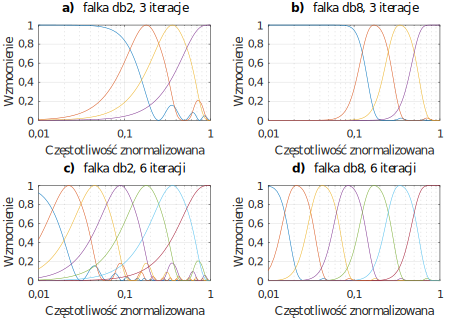
\includegraphics{obrazki/bank_db_demo}
\makecaption{fig:demo_db}{Przykładowe banki filtrów dla rodziny falek \enquote{Daubechies}}
\end{center}
\end{figure}

Przedstawiona na osi pionowej maksymalna wartość wzmocnienia w funkcji częstotliwości sygnału może być w rzeczywistości większa od jedności. W praktyce każdy z fragmentów banku filtrów traktować można jako pasmowo-przepustowy filtr cyfrowy i opisywać za pomocą modelu filtru o skończonej odpowiedzi impulsowej (\enquote{FIR}). Z punktu widzenia pojedynczej wielkości wyjściowej, algorytm transformacji falkowej może być zatem rozumiany jako odpowiednio zaprojektowany filtr, który z sygnału wejściowego przenosi na wyjście wybrane harmoniczne sygnału wejściowego z odpowiednim wzmocnieniem i przesunięciem fazowym. Przedstawione cechy banku filtrów będą bardzo istotne w dalszym etapie pracy w szczególności do określania, w jaki sposób algorytm przenosi błędy opisane w pracy jako dynamiczne. Należy zauważyć, że skoro kolejne filtry w banku odpowiadają kolejnym etapom dekompozycji sygnału, to w większości przypadków właściwości metrologiczne będą jednakowe dla wszystkich wielkości wyjściowych powiązanych z identycznym etapem dekompozycji sygnału, co znacznie upraszcza proces analizy właściwości metrologicznych omawianych algorytmów. Należy jednak mieć na uwadze, że w pewnych przypadkach wypadkowe właściwości toru pomiarowego mogą ulec zmianie, jeżeli wprowadzona zostanie dodatkowa modyfikacja wielkości wejściowych algorytmu transformacji falkowej (np. wprowadzone zostanie okno pomiarowe). Należy w takim przypadku analizować właściwości metrologiczne każdej wielkości wyjściowej z osobna, a nie, jak w klasycznym przypadku, analizować je zbiorczo dla danego etapu dekompozycji.

\begin{figure}[htb!]
\begin{center}
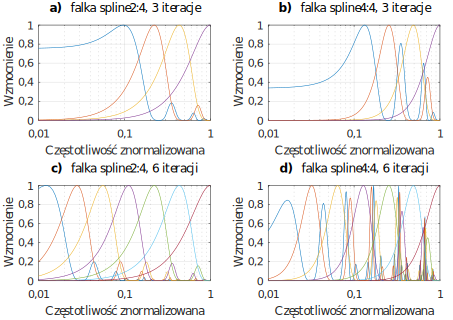
\includegraphics{obrazki/bank_spline_demo}
\makecaption{fig:demo_spline}{Przykładowe banki filtrów dla rodziny falek \enquote{Spline}}
\end{center}
\end{figure}

\section{Macierzowa postać algorytmu}

Ze względu na bardzo dużą liczbę opisanych w literaturze falek~\cite{akujuobi_applications}, ich unikatowe właściwości oraz możliwość zmiany parametrów procesu dekompozycji sygnału, metody analityczne określenia właściwości metrologicznych dla wybranej kombinacji parametrów okazują się czasochłonne i niepraktyczne~\cite{yan_uncertainty, wilczok_uncertainty, peretto_uncertainty, sarrafi_uncertainty}. \DIFdelbegin \DIFdel{Część opisywanych w literaturze falek obejmuje falki }\DIFdelend \DIFaddbegin \DIFadd{Opisywane w literaturze falki obejmują między innymi rodziny}\DIFaddend : \enquote{Daubechies}~\cite{vonesch_dbbasics}, \enquote{Haara}~\cite{stankovic_haar}, \enquote{Coiflet}~\cite{wei_coiflet}, \enquote{Biortogonalne}~\cite{sweldens_bior}, \enquote{Morleta}~\cite{cohen_morlet}, \enquote{Meksykańskiej czapki}~\cite{singh_mexican}, \DIFaddbegin \DIFadd{oraz }\DIFaddend \enquote{Spline}~\cite{averbuch_spline, wang_splinebasics}. Każdą falkę oraz przypisaną do niej funkcję skalującą opisują odpowiednie równania, przy czym nie zawsze są one przedstawiane w postaci jawnej -- w wielu przypadkach rodzina falek opisana jest przez zbiór zależności określających wymagane przez nią założenia, co jeszcze bardziej komplikuje proces analizy tych algorytmów~\cite{rowe_dbmath}. Podczas projektowania toru pomiarowego często istnieje potrzeba zmiany parametrów algorytmu transformacji falkowej, co pociąga za sobą konieczność przeprowadzenia powtórnej analizy jego właściwości metrologicznych. Wszystkie te czynniki sprawiają, że analiza ta jest najczęściej pomijana w pracach opisujących aplikacje omawianych algorytmów. Z opisywanych właściwości algorytmów transformacji falkowej wynika potrzeba przedstawienia uniwersalnej metody umożliwiającej analizę właściwości metrologicznych tych algorytmów. Metoda ta musi być przystępna w aplikacji oraz musi zakładać, że projektant toru pomiarowego nie jest ekspertem w dziedzinie transformacji falkowej, a jedynie jej użytkownikiem. Co więcej, ewentualna zmiana parametrów zastosowanego algorytmu nie może być kłopotliwa z punktu widzenia określenia nowych właściwości metrologicznych analizowanego algorytmu.

Problem skomplikowanej analizy algorytmów transformacji falkowej, podobnie jak w przypadku innych algorytmów przetwarzających ciągi danych, uprościć można przedstawiając analizowany algorytm w postaci macierzowej~\cite{jakubiec_algorithms, jakubiec_system}. Wektor wielkości wyjściowych algorytmu jest w omawianym przypadku równy iloczynowi macierzy transformacji i wektora wielkości wejściowych, co opisano równaniem~\eqref{eq:alg_out_mat}. Przedstawienie algorytmu transformacji falkowej w formie macierzowej \DIFdelbegin \DIFdel{umożliwa }\DIFdelend \DIFaddbegin \DIFadd{umożliwia }\DIFaddend stworzenie jednolitego i uniwersalnego opisu działania tego algorytmu oraz w znaczącym stopniu \DIFdelbegin \DIFdel{ułatwa }\DIFdelend \DIFaddbegin \DIFadd{ułatwia }\DIFaddend jego analizę w kolejnych rozdziałach pracy. Zwykle projektant toru pomiarowego nie jest ekspertem w dziedzinie algorytmów transformacji falkowej -- jest on ekspertem w dziedzinie analizowanego zjawiska, a transformacja falkowa jest dla niego jedynie narzędziem, umożliwiającym jego analizę. Stąd, w większości przypadków, osoba ta stosuje gotowe biblioteki zaimplementowane np. dla środowisk \enquote{Matlab}, \enquote{GNU Octave} czy \enquote{PyWavelets}~\cite{lee_pywavelets, misiti_matlabwav}.

W celu identyfikacji wartości współczynników macierzy transformacji należy zastosować metodę opisaną w poprzednim rozdziale pracy lub wyznaczyć te wartości analitycznie, co przedstawiono w dalszej cześć rozdziału. Opisany wcześniej algorytm identyfikacji macierzy transformacji może być wykorzystany w środowiskach, które implementują algorytmy transformacji falkowej, przez co projektant toru pomiarowego z łatwością jest w stanie go zastosować. Ewentualna zmiana parametrów algorytmu transformacji falkowej (zmiana liczby wielkości wejściowych, liczby iteracji procesu dekompozycji, czy wybór innej falki-matki) skutkować będzie jedynie koniecznością ponownej identyfikacji wartości współczynników macierzy transformacji.

Poza opisanym algorytmem identyfikacji współczynników macierzy transformacji, bazującym na istniejącej implementacji omawianego algorytmu, istnieje możliwość wyznaczenia wartości tych współczynników przy użyciu zależności przedstawionych we wcześniejszej części rozdziału, opisującej właściwości algorytmu dyskretnej transformacji falkowej. Proces ten jest jednak skomplikowany i uzależniony od założeń związanych z opisem zastosowanej falki-matki i jej funkcji skalującej. Poniżej przedstawiono przykład wyznaczania wartości macierzy transformacji w przypadku zastosowania falki \enquote{db2} dla dwóch iteracji procesu dekompozycji sygnału oraz ośmiu próbek wejściowych sygnału. Macierz transformacji analizowanego algorytmu składa się zatem z $M = 8$ wierszy\DIFdelbegin \DIFdel{i }\DIFdelend \DIFaddbegin \DIFadd{, co wynika z liczby wielkości wyjściowych algorytmu oraz }\DIFaddend $N = 8$ kolumn, \DIFdelbegin \DIFdel{zatem wektory }\DIFdelend \DIFaddbegin \DIFadd{co wynika z liczby }\DIFaddend wielkości wejściowych\DIFdelbegin \DIFdel{oraz wyjściowych składają się z $M = N = 8$ elementów}\DIFdelend .

Rodzina falek \enquote{Daubechies} (nazywana w skrócie \enquote{db}) została opisana przez Ingrid Daubechies w 1987 roku. Rodzina ta cechuje się ortogonalnością, natomiast nie wykazuje cech symetrii. Poza założeniami opisanymi w poprzednim podrozdziale, danymi w równaniach~\eqref{eq:dwt_orthogonal_mather} oraz od~\eqref{eq:dwt_orthogonal_father} do~\eqref{eq:dwt_scalemulort}, rodzina ta spełnia dodatkowe założenie odnośnie relacji pomiędzy kolejnymi współczynnikami skalującymi, które opisuje następujące równanie~\cite{vonesch_dbbasics}:
\begin{equation}
\sum _{k=0} ^{N_k-1} \emb{-1}^{k} c_{k} k^{m} = 0 \label{eq:db_musthave},
\end{equation}
gdzie $m$ jest liczbą całkowitą z przedziału \DIFdelbegin \DIFdel{$<0;\frac{N_{k}}{2}-1>$}\DIFdelend \DIFaddbegin \DIFadd{$\interval{0}{\frac{N_{k}}{2}-1}$}\DIFaddend . W przypadku falek \enquote{db} oraz ich pochodnych \DIFdelbegin \DIFdel{, }\DIFdelend rząd falki wynosi $\frac{N_{k}}{2}$. Falka \enquote{db2}, będąca falką drugiego rzędu, posiada zatem cztery niezerowe współczynniki skalujące. W literaturze spotkać się można również z oznaczeniem \enquote{D4} dla omawianej falki, gdzie zamiast rzędu falki wskazana jest liczba niezerowych współczynników skalujących. Należy zauważyć, że falka \enquote{Daubechies} rzędu pierwszego jest opisana identycznymi zależnościami, jak falka Hara i posiada identyczne właściwości. Z falek \enquote{Daubechies} wywodzą się kolejne rodziny: \enquote{Symleth} oraz \enquote{Coiflet}, które uzupełniają ją o kolejne cechy -- w szczególności symetrię, istotną podczas przetwarzania i analizy obrazów~\cite{wallen_handbook, akujuobi_applications}.

Jako, że falka \enquote{db2} posiada cztery niezerowe współczynniki skalujące oznaczone jako $c_0$, $c_1$, $c_2$, $c_3$, to zgodnie z równaniem~\eqref{eq:dwt_scalefunrek} oraz równaniem~\eqref{eq:dwt_waveletfunrek}, zapisać można równanie falki-matki i funkcji skalującej w postaci:
\begin{gather}
\phi \emb{t} = c_{0} \phi \emb{2t} + c_{1} \phi \left( 2t - 1 \right) + c_{2} \phi \left( 2t - 2 \right) + c_{3} \phi \left( 2t - 3 \right) \label{eq:db2_scalefunrek}, \\
\psi \emb{t} = c_{3} \phi \emb{2t} - c_{2} \phi \left( 2t - 1 \right) + c_{1} \phi \left( 2t - 2 \right) - c_{0} \phi \left( 2t - 3 \right) \label{eq:db2_waveletfunrek}.
\end{gather}
Uwzględniając założenia przedstawione w poprzedniej części rozdziału oraz te wskazane powyżej, zapisać można układ równań wiążący wszystkie przedstawione zależności:
\begin{equation}
\begin{cases}
	c_{0} + c_{1} + c_{2} + c_{3} = 2                 & $na podstawie właściwości~\eqref{eq:dwt_scalefunsum}$ \\
	c_{0}^{2} + c_{1}^{2} + c_{2}^{2} + c_{3}^{2} = 2 & $na podstawie właściwości~\eqref{eq:dwt_scalemulort}$ \\
	c_{0} - c_{1} + c_{2} - c_{3} = 0                 & $na podstawie~\eqref{eq:db_musthave} dla $ m = 0 \\
	- 1 c_{1} + 2 c_{2} - 3 c_{3} = 0                 & $na podstawie~\eqref{eq:db_musthave} dla $ m = 1
\end{cases}
\label{eq:db2_system},
\end{equation}
oraz wskazać jego rozwiązanie, które determinuje następujące wartości kolejnych współczynników skalujących:
\begin{equation}
c_{0} = \frac{1 + \sqrt{3}}{4}, c_{1} = \frac{3 + \sqrt{3}}{4}, c_{2} = \frac{3 - \sqrt{3}}{4}, c_{3} = \frac{1 - \sqrt{3}}{4} \label{eq:db2_coefs},
\end{equation}
przy czym analogicznie postąpić należy w przypadku wyższych rzędów opisywanej falki.

Zgodnie z założeniami odnośnie długości wektora wielkości wejściowych oraz liczby poziomów dekompozycji zauważyć można, że wektor wielkości wyjściowych zawierać będzie dwie próbki związane z aproksymacją sygnału dla skali $m = 2$, dwie próbki związane z detalami sygnału dla skali $m = 2$ oraz cztery próbki związane z detalami dla skali $m = 1$. Oznaczając wektor wielkości wejściowych jako:
\begin{equation}
\mathbf{x}^{T} =
\begin{bmatrix}
S_{0,0} & S_{0,1} & S_{0,2} & S_{0,3} & S_{0,4} & S_{0,5} & S_{0,6} & S_{0,7}
\end{bmatrix}
\label{eq:db2_invect},
\end{equation}
wektor wielkości wyjściowych można opisać w postaci:
\begin{equation}
\mathbf{X}^{T} =
\begin{bmatrix}
S_{2,0} & S_{2,1} & T_{2,0} & T_{2,1} & T_{1,0} & T_{1,1} & T_{1,2} & T_{1,3}
\end{bmatrix}
\label{eq:db2_outvect},
\end{equation}
a następnie zgodnie z równaniem~\eqref{eq:dwt_aproxrek} oraz~\eqref{eq:dwt_detailrek} opisać można kolejne wymienione w równaniu~\eqref{eq:db2_outvect} wielkości wyjściowe za pomocą zależności:
\begin{gather}
S_{2,0} = \frac{1}{\sqrt{2}} \left( c_{0} S_{1,0} + c_{1} S_{1,1} + c_{2} S_{1,2} + c_{3} S_{1,3} \right) \label{eq:db2_outvect_s_2_0}, \\
S_{2,1} = \frac{1}{\sqrt{2}} \left( c_{0} S_{1,2} + c_{1} S_{1,3} + c_{2} S_{1,4} + c_{3} S_{1,5} \right) \label{eq:db2_outvect_s_2_1}, \\
T_{2,0} = \frac{1}{\sqrt{2}} \left( c_{3} S_{1,0} - c_{2} S_{1,1} + c_{1} S_{1,2} - c_{0} S_{1,3} \right) \label{eq:db2_outvect_t_2_0}, \\
T_{2,1} = \frac{1}{\sqrt{2}} \left( c_{3} S_{1,2} - c_{2} S_{1,3} + c_{1} S_{1,4} - c_{0} S_{1,5} \right) \label{eq:db2_outvect_t_2_1}, \\
T_{1,0} = \frac{1}{\sqrt{2}} \left( c_{3} S_{0,0} - c_{2} S_{0,1} + c_{1} S_{0,2} - c_{0} S_{0,3} \right) \label{eq:db2_outvect_t_1_0}, \\
T_{1,1} = \frac{1}{\sqrt{2}} \left( c_{3} S_{0,2} - c_{2} S_{0,3} + c_{1} S_{0,4} - c_{0} S_{0,5} \right) \label{eq:db2_outvect_t_1_1}, \\
T_{1,2} = \frac{1}{\sqrt{2}} \left( c_{3} S_{0,4} - c_{2} S_{0,5} + c_{1} S_{0,6} - c_{0} S_{0,7} \right) \label{eq:db2_outvect_t_1_2}, \\
T_{1,3} = \frac{1}{\sqrt{2}} \left( c_{3} S_{0,6} - c_{2} S_{0,7} + c_{1} S_{0,0} - c_{0} S_{0,1} \right) \label{eq:db2_outvect_t_1_3},
\end{gather}
gdzie symbol $S_{m,n}$ oznacza aproksymacje, natomiast $T_{m,n}$ detale sygnału dla zadanego numeru skali i numeru przesunięcia w czasie. Po przekształceniu otrzymuje się równania:
\begin{gather}
\begin{split}
S_{2,0} =~
	& \frac{1}{\sqrt{2}} \frac{c_{0}}{\sqrt{2}} \left( c_{0} S_{0,0} + c_{1} S_{0,1} + c_{2} S_{0,2} + c_{3} S_{0,3} \right) + \\
	& \frac{1}{\sqrt{2}} \frac{c_{1}}{\sqrt{2}} \left( c_{0} S_{0,2} + c_{1} S_{0,3} + c_{2} S_{0,4} + c_{3} S_{0,5} \right) + \\
	& \frac{1}{\sqrt{2}} \frac{c_{2}}{\sqrt{2}} \left( c_{0} S_{0,4} + c_{1} S_{0,5} + c_{2} S_{0,6} + c_{3} S_{0,7} \right) + \\
	& \frac{1}{\sqrt{2}} \frac{c_{3}}{\sqrt{2}} \left( c_{0} S_{0,6} + c_{1} S_{0,7} + c_{2} S_{0,0} + c_{3} S_{0,1} \right)
\end{split}
\label{eq:db2_outvect_s_2_0_rek}, \\
\begin{split}
S_{2,1} =~
	& \frac{1}{\sqrt{2}} \frac{c_{0}}{\sqrt{2}} \left( c_{0} S_{0,4} + c_{1} S_{0,5} + c_{2} S_{0,6} + c_{3} S_{0,7} \right) + \\
	& \frac{1}{\sqrt{2}} \frac{c_{1}}{\sqrt{2}} \left( c_{0} S_{0,6} + c_{1} S_{0,7} + c_{2} S_{0,0} + c_{3} S_{0,1} \right) + \\
	& \frac{1}{\sqrt{2}} \frac{c_{2}}{\sqrt{2}} \left( c_{0} S_{0,0} + c_{1} S_{0,1} + c_{2} S_{0,2} + c_{3} S_{0,3} \right) + \\
	& \frac{1}{\sqrt{2}} \frac{c_{3}}{\sqrt{2}} \left( c_{0} S_{0,2} + c_{1} S_{0,3} + c_{2} S_{0,4} + c_{3} S_{0,5} \right)
\end{split}
\label{eq:db2_outvect_s_2_1_rek}, \\
\begin{split}
T_{2,0} =~
	& \frac{1}{\sqrt{2}} \frac{c_{3}}{\sqrt{2}} \left( c_{0} S_{0,0} + c_{1} S_{0,1} + c_{2} S_{0,2} + c_{3} S_{0,3} \right) - \\
	& \frac{1}{\sqrt{2}} \frac{c_{2}}{\sqrt{2}} \left( c_{0} S_{0,2} + c_{1} S_{0,3} + c_{2} S_{0,4} + c_{3} S_{0,5} \right) + \\
	& \frac{1}{\sqrt{2}} \frac{c_{1}}{\sqrt{2}} \left( c_{0} S_{0,4} + c_{1} S_{0,5} + c_{2} S_{0,6} + c_{3} S_{0,7} \right) - \\
	& \frac{1}{\sqrt{2}} \frac{c_{0}}{\sqrt{2}} \left( c_{0} S_{0,6} + c_{1} S_{0,7} + c_{2} S_{0,0} + c_{3} S_{0,1} \right)
\end{split}
\label{eq:db2_outvect_t_2_0_rek}, \\
\begin{split}
T_{2,1} =~
	& \frac{1}{\sqrt{2}} \frac{c_{3}}{\sqrt{2}} \left( c_{0} S_{0,4} + c_{1} S_{0,5} + c_{2} S_{0,6} + c_{3} S_{0,7} \right) - \\
	& \frac{1}{\sqrt{2}} \frac{c_{2}}{\sqrt{2}} \left( c_{0} S_{0,6} + c_{1} S_{0,7} + c_{2} S_{0,0} + c_{3} S_{0,1} \right) + \\
	& \frac{1}{\sqrt{2}} \frac{c_{1}}{\sqrt{2}} \left( c_{0} S_{0,0} + c_{1} S_{0,1} + c_{2} S_{0,2} + c_{3} S_{0,3} \right) - \\
	& \frac{1}{\sqrt{2}} \frac{c_{0}}{\sqrt{2}} \left( c_{0} S_{0,2} + c_{1} S_{0,3} + c_{2} S_{0,4} + c_{3} S_{0,5} \right)
\end{split}
\label{eq:db2_outvect_t_2_1_rek}.
\end{gather}
Grupując odpowiednie wyrazy w zależnościach od~\eqref{eq:db2_outvect_s_2_0_rek} do~\eqref{eq:db2_outvect_t_2_1_rek}, a następnie podstawiając $S_{0,i} = x_{i} = x(i)$, otrzymuje się:
\begin{gather}
\begin{split}
S_{2,0} =~
	& \frac{c_{0}^{2} + c_{2} c_{3}}{2} x_{0} + \frac{c_{0} c_{1} + c_{3}^{2}}{2} x_{1} + \frac{c_{0} c_{2} + c_{0} c_{1}}{2} x_{2} + \frac{c_{0} c_{3} + c_{1}^{2}}{2} x_{3} + \\
	& \frac{c_{1} c_{2} + c_{0} c_{2}}{2} x_{4} + \frac{c_{1} c_{3} + c_{1} c_{2}}{2} x_{5} + \frac{c_2^{2} + c_{0} c_{3}}{2} x_{6} + \frac{c_{2} c_{3} + c_{1} c_{3}}{2} x_7
\end{split}
\label{eq:db2_outvect_s_2_0_full}, \\
\begin{split}
S_{2,1} =~
	& \frac{c_{1} c_{2} + c_{0} c_{2}}{2} x_{0} + \frac{c_{1} c_{3} + c_{1} c_{2}}{2} x_{1} + \frac{c_2^{2} + c_{0} c_{3}}{2} x_{2} + \frac{c_{2} c_{3} + c_{1} c_{3}}{2} x_{3} + \\
	& \frac{c_0^{2} + c_{2} c_{3}}{2} x_{4} + \frac{c_{0} c_{1} + c_3^{2}}{2} x_{5} + \frac{c_{0} c_{2} + c_{0} c_{1}}{2} x_{6} + \frac{c_{0} c_{3} + c_1^{2}}{2} x_7
\end{split}
\label{eq:db2_outvect_s_2_1_full}, \\
\begin{split}
T_{2,0} =~
	& \frac{c_{0} c_{3} - c_{0} c_{2}}{2} x_{0} + \frac{c_{1} c_{3} - c_{0} c_{3}}{2} x_{1} + \frac{c_{2} c_{3} - c_{0} c_{2}}{2} x_{2} + \frac{c_3^{2} - c_{1} c_{2}}{2} x_{3} + \\
	& \frac{c_{0} c_{1} - c_2^{2}}{2} x_{4} + \frac{c_1^{2} - c_{2} c_{3}}{2} x_{5} + \frac{c_{1} c_{2} - c_0^{2}}{2} x_{6} + \frac{c_{1} c_{3} - c_{0} c_{1}}{2} x_7
\end{split}
\label{eq:db2_outvect_t_2_0_full}, \\
\begin{split}
T_{2,1} =~
	& \frac{c_{0} c_{1} - c_2^{2}}{2} x_{0} + \frac{c_1^{2} - c_{2} c_{3}}{2} x_{1} + \frac{c_{1} c_{2} - c_0^{2}}{2} x_{2} + \frac{c_{1} c_{3} - c_{0} c_{1}}{2} x_{3} + \\
	& \frac{c_{0} c_{3} - c_{0} c_{2}}{2} x_{4} + \frac{c_{1} c_{3} - c_{0} c_{3}}{2} x_{5} + \frac{c_{2} c_{3} - c_{0} c_{2}}{2} x_{6} + \frac{c_3^{2} - c_{1} c_{2}}{2} x_7
\end{split}
\label{eq:db2_outvect_t_2_1_full}, \\
T_{1,0} =
	\frac{c_{3}}{\sqrt{2}} x_{0} + \frac{- c_{2}}{\sqrt{2}} x_{1} + \frac{c_{1}}{\sqrt{2}} x_{2} + \frac{- c_{0}}{\sqrt{2}} x_{3} +
	\frac{0}{\sqrt{2}} x_{4} + \frac{0}{\sqrt{2}} x_{5} + \frac{0}{\sqrt{2}} x_{6} + \frac{0}{\sqrt{2}} x_{7}
\label{eq:db2_outvect_t_1_0_full}, \\
T_{1,1} =
	\frac{0}{\sqrt{2}} x_{0} + \frac{0}{\sqrt{2}} x_{1} + \frac{c_{3}}{\sqrt{2}} x_{2} + \frac{- c_{2}}{\sqrt{2}} x_{3} +
	\frac{c_{1}}{\sqrt{2}} x_{4} + \frac{- c_{0}}{\sqrt{2}} x_{5} + \frac{0}{\sqrt{2}} x_{6} + \frac{0}{\sqrt{2}} x_{7}
\label{eq:db2_outvect_t_1_1_full}, \\
T_{1,2} =
	\frac{0}{\sqrt{2}} x_{0} + \frac{0}{\sqrt{2}} x_{1} + \frac{0}{\sqrt{2}} x_{2} + \frac{0}{\sqrt{2}} x_{3} +
	\frac{c_{3}}{\sqrt{2}} x_{4} + \frac{- c_{2}}{\sqrt{2}} x_{5} + \frac{c_{1}}{\sqrt{2}} x_{6} + \frac{- c_{0}}{\sqrt{2}} x_{7}
\label{eq:db2_outvect_t_1_2_full}, \\
T_{1,3} =
	\frac{c_{1}}{\sqrt{2}} x_{0} + \frac{- c_{0}}{\sqrt{2}} x_{1} + \frac{0}{\sqrt{2}} x_{2} + \frac{0}{\sqrt{2}} x_{3} +
	\frac{0}{\sqrt{2}} x_{4} + \frac{0}{\sqrt{2}} x_{5} + \frac{c_{3}}{\sqrt{2}} x_{6} + \frac{- c_{2}}{\sqrt{2}} x_{7}
\label{eq:db2_outvect_t_1_3_full}.
\end{gather}
Następnie, uwzględniając w równaniu~\eqref{eq:alg_out_mat} kolejność elementów wektora wielkości wyjściowych zgodną z założoną w równaniu~\eqref{eq:db2_outvect}, zapisać można:
\begin{gather}
S_{2,0} = a_{0,0} x_{0} + a_{0,1} x_{1} + a_{0,2} x_{2} + a_{0,3} x_{3} + a_{0,4} x_{4} + a_{0,5} x_{5} + a_{0,6} x_{6} + a_{0,7} x_{7} \label{eq:db2_outvect_s_2_0_row}, \\
S_{2,1} = a_{1,0} x_{0} + a_{1,1} x_{1} + a_{1,2} x_{2} + a_{1,3} x_{3} + a_{1,4} x_{4} + a_{1,5} x_{5} + a_{1,6} x_{6} + a_{1,7} x_{7} \label{eq:db2_outvect_s_2_1_row}, \\
T_{2,0} = a_{2,0} x_{0} + a_{2,1} x_{1} + a_{2,2} x_{2} + a_{2,3} x_{3} + a_{2,4} x_{4} + a_{2,5} x_{5} + a_{2,6} x_{6} + a_{2,7} x_{7} \label{eq:db2_outvect_t_2_0_row}, \\
T_{2,1} = a_{3,0} x_{0} + a_{3,1} x_{1} + a_{3,2} x_{2} + a_{3,3} x_{3} + a_{3,4} x_{4} + a_{3,5} x_{5} + a_{3,6} x_{6} + a_{3,7} x_{7} \label{eq:db2_outvect_t_2_1_row}, \\
T_{1,0} = a_{4,0} x_{0} + a_{4,1} x_{1} + a_{4,2} x_{2} + a_{4,3} x_{3} + a_{4,4} x_{4} + a_{4,5} x_{5} + a_{4,6} x_{6} + a_{4,7} x_{7} \label{eq:db2_outvect_t_1_0_row}, \\
T_{1,1} = a_{5,0} x_{0} + a_{5,1} x_{1} + a_{5,2} x_{2} + a_{5,3} x_{3} + a_{5,4} x_{4} + a_{5,5} x_{5} + a_{5,6} x_{6} + a_{5,7} x_{7} \label{eq:db2_outvect_t_1_1_row}, \\
T_{1,2} = a_{6,0} x_{0} + a_{6,1} x_{1} + a_{6,2} x_{2} + a_{6,3} x_{3} + a_{6,4} x_{4} + a_{6,5} x_{5} + a_{6,6} x_{6} + a_{6,7} x_{7} \label{eq:db2_outvect_t_1_2_row}, \\
T_{1,3} = a_{7,0} x_{0} + a_{7,1} x_{1} + a_{7,2} x_{2} + a_{7,3} x_{3} + a_{7,4} x_{4} + a_{7,5} x_{5} + a_{7,6} x_{6} + a_{7,7} x_{7} \label{eq:db2_outvect_t_1_3_row}.
\end{gather}

Powyższe zależności pozwalają wyznaczyć wartości współczynników macierzy transformacji dla analizowanego algorytmu dyskretnej transformacji falkowej. Po podstawieniu wartości zgodnie z zależnością~\eqref{eq:db2_coefs} oraz biorąc pod uwagę równania od~\eqref{eq:db2_outvect_s_2_0_row} do~\eqref{eq:db2_outvect_t_1_3_row} macierz transformacji przyjmuje postać:
\begin{equation}
\mathbf{A} =
\begin{bmatrix}
\frac{5 - \sqrt{3}}{16} & \frac{5 + \sqrt{3}}{16} & \frac{3 + 3 \sqrt{3}}{16} & \frac{5 + 3 \sqrt{3}}{16} & \frac{3 + \sqrt{3}}{16} & \frac{3 - \sqrt{3}}{16} & \frac{5 - 3 \sqrt{3}}{16} & \frac{3 - 3 \sqrt{3}}{16} \\
\frac{3 + \sqrt{3}}{16} & \frac{3 - \sqrt{3}}{16} & \frac{5 - 3 \sqrt{3}}{16} & \frac{3 - 3 \sqrt{3}}{16} & \frac{5 - \sqrt{3}}{16} & \frac{5 + \sqrt{3}}{16} & \frac{3 + 3 \sqrt{3}}{16} & \frac{5 + 3 \sqrt{3}}{16} \\
- \frac{1 + \sqrt{3}}{16} & \frac{1 - \sqrt{3}}{16} & \frac{3 - 3 \sqrt{3}}{16} & - \frac{1 + \sqrt{3}}{16} & - \frac{3 - 5 \sqrt{3}}{16} & \frac{3 + 5 \sqrt{3}}{16} & \frac{1 - \sqrt{3}}{16} & - \frac{3 + 3 \sqrt{3}}{16} \\
- \frac{3 - 5 \sqrt{3}}{16} & \frac{3 + 5 \sqrt{3}}{16} & \frac{1 - \sqrt{3}}{16} & - \frac{3 + 3 \sqrt{3}}{16} & - \frac{1 + \sqrt{3}}{16} & \frac{1 - \sqrt{3}}{16} & \frac{3 - 3 \sqrt{3}}{16} & - \frac{1 + \sqrt{3}}{16} \\
\frac{1 - \sqrt{3}}{4 \sqrt{2}} & - \frac{3 - \sqrt{3}}{4 \sqrt{2}} & \frac{3 + \sqrt{3}}{4 \sqrt{2}} & - \frac{1 + \sqrt{3}}{4 \sqrt{2}} & 0 & 0 & 0 & 0 \\
0 & 0 & \frac{1 - \sqrt{3}}{4 \sqrt{2}} & - \frac{3 - \sqrt{3}}{4 \sqrt{2}} & \frac{3 + \sqrt{3}}{4 \sqrt{2}} & - \frac{1 + \sqrt{3}}{4 \sqrt{2}} & 0 & 0 \\
0 & 0 & 0 & 0 & \frac{1 - \sqrt{3}}{4 \sqrt{2}} & - \frac{3 - \sqrt{3}}{4 \sqrt{2}} & \frac{3 + \sqrt{3}}{4 \sqrt{2}} & - \frac{1 + \sqrt{3}}{4 \sqrt{2}} \\
\frac{3 + \sqrt{3}}{4 \sqrt{2}} & - \frac{1 + \sqrt{3}}{4 \sqrt{2}} & 0 & 0 & 0 & 0 & \frac{1 - \sqrt{3}}{4 \sqrt{2}} & - \frac{3 - \sqrt{3}}{4 \sqrt{2}}
\end{bmatrix}
\label{eq:db2_2_8_matrix}.
\end{equation}
W analogiczny sposób wyznaczyć można wartości elementów macierzy transformacji dla innej liczby wielkości wejściowych algorytmu oraz dowolnej liczby poziomów dekompozycji. W przypadku zastosowania innych rodzin falek należy zastosować odpowiednie dla nich założenia i na ich podstawie wyznaczyć kolejne wielkości niezbędne do określenia wartości elementów identyfikowanej macierzy, przy czym procedura ta przebiega podobnie, jak przedstawiono w powyższym przykładzie.

\section{Przenoszenie błędów przez algorytm}

Jako, że algorytm transformacji falkowej przedstawić można w formie macierzowej, istnieje możliwość analizy jego właściwości metrologicznych zgodnie z metodą przedstawioną w poprzednim rozdziale pracy. Należy zauważyć, że parametry macierzy transformacji wynikające z charakterystyki zastosowanej falki-matki są kluczowym czynnikiem mającym wpływ na związek pomiędzy wariancją błędu analizowanej wielkości wyjściowej, a wariancją błędu wielkości wejściowych~\cite{auth_electronics}. Zgodnie z centralnym twierdzeniem granicznym, bez względu na rozkład błędów losowych wielkości wejściowych algorytmu, kształt rozkładu błędu losowego będzie zbliżony do rozkładu normalnego~\cite{jcgm_guide}. Powyższe założenie jest prawdziwe wtedy, gdy algorytm przetwarza wielokrotnie błędy losowe o tych samych parametrach.

Analizując macierz transformacji przedstawioną w równaniu~\eqref{eq:db2_2_8_matrix} zauważyć można, że jest ona podzielona z punktu widzenia wierszy na kilka charakterystycznych obszarów, przy czym ich liczba zależna jest od liczby iteracji procesu dekompozycji sygnału. Każdy z obszarów odpowiada kolejnemu wyjściu algorytmu Malata, który przedstawiono wcześniej na rysunku~\ref{fig:dwt_decomposition}. W obrębie danego obszaru kolejne wartości współczynników macierzy pozostają niezmienne, przy czym ich pozycje są przesunięte o dwie kolumny w prawo w stosunku do wiersza poprzedniego. Zjawisko to wynika z przesunięcia okna pomiarowego (zmiany parametru przesunięcia falki), natomiast liczba kolumn, o którą przesunięta jest pozycja każdego współczynnika, wynika z przeprowadzenia procesu decymacji (do druga wartość jest odrzucana). Z punktu widzenia analizy metrologicznej zauważyć można, że wielkości wyjściowe związane z tym samym parametrem skali mogą być analizowane równocześnie, gdyż odpowiada im filtr o tych samych parametrach, przez co wartości wielkości opisanych w równaniach~\eqref{eq:alg_trans_stat} oraz~\eqref{eq:alg_trans_rand} będą identyczne~\cite{auth_electronics}.

W przypadku falek z rodziny \enquote{Daubechies}, a także ich pochodnych \enquote{Symleth} oraz \enquote{Coiflets}, niezależnie od liczby poziomów dekompozycji, wartość współczynnika $A_{r,i}$ dla wszystkich wielkości wyjściowych każdorazowo wynosić będzie~\num{1}, natomiast wartość współczynnika $A_{s,i}$ dla aproksymacji sygnału wynosić będzie~\num{2}. Zależności te wynikają bezpośrednio z równań~\eqref{eq:dwt_scalefunsum} oraz~\eqref{eq:db_musthave}~\cite{vonesch_dbbasics, wei_coiflet}. Nie oznacza to jednak, że dalsza analiza może zostać pominięta, a algorytm transformacji falkowej nie ma wpływu na przenoszone błędy wielkości wejściowych, ponieważ wciąż istnieje potrzeba analizy pozostałych rodzajów błędów. Ze względu na fakt, że tylko jedna grupa wielkości wyjściowych, związana z aproksymacją sygnału, stanowić będzie filtr dolno-przepustowy, dla pozostałych grup wielkości wyjściowych wartość współczynnika $A_{s,i}$ będzie zwykle zerowa. Wynika to z faktu, że błędy statyczne stanowią składową stałą sygnału, a zatem nie będą przenoszone przez filtry inne, niż dolno-przepustowe.

\section{Błędy własne algorytmu}

Analizując przykładową macierz transformacji przedstawioną w równaniu~\eqref{eq:db2_2_8_matrix}, której wartości wyznaczono we wcześniejszej części rozdziału, zauważyć można, że wszystkie niezerowe wartości elementów tej macierzy są niewymierne. Niewymierność ta jest pierwszym powodem powstawania błędu własnego zaokrągleń, którym obarczone będą wyznaczane numerycznie wielkości wyjściowe algorytmu dyskretnej transformacji falkowej. Kolejnym źródłem błędów będą zaokrąglenia wynikające z ograniczonej precyzji liczb, przeprowadzane podczas wykonywania operacji mnożenia i dodawania. Błędy te, zgodnie ze wcześniej wprowadzonym podziałem, zaliczyć można do błędów losowych ponieważ nie ma możliwości deterministycznego opisu przebiegu sygnału tych błędów, a dodatkowo ich realizacje będą zmienne w obrębie okna pomiarowego.

Zakładając, że analizowana $j$-ta wielkość wyjściowa algorytmu obarczona jest jedynie błędem własnym, który wynika z omówionych w poprzednim akapicie zjawisk, sygnał $e_{X,z}(j)$ związany z tym błędem zdefiniować można w postaci:
\begin{equation}
e_{X,z} \emb{j} = \tilde{X} \emb{j} - \dot{X} \emb{j} \label{eq:fwt_outerr_self}.
\end{equation}
Należy zauważyć, że zależność~\eqref{eq:fwt_outerr_self} jest prawdziwa tylko wtedy, gdy wielkości wejściowe $x(i)$ algorytmu nie są obarczone żadnymi błędami, tj. dla $\tilde{x}(i) = \dot{x}(i)$. Dodatkowo zakłada się, że w przypadku algorytmu idealnego sygnały błędu własnego $e_{X,z}(j)$ nie występują, a zatem dla takiego algorytmu zachodzi $e_{X,z}(j) = 0$.

Parametry rozkładu sygnałów błędów własnych kolejnych wielkości wyjściowych algorytmu wyznaczyć można eksperymentalnie, stosując metodę Monte-Carlo~\cite{jcgm_montecarlo}. Należy w tym celu wielokrotnie podawać na wejście algorytmu wektor wielkości wejściowych, którego wartości kolejnych elementów będą liczbami losowymi. Schemat blokowy pojedynczej iteracji omawianego eksperymentu przedstawia rysunek~\ref{fig:schemat_dwt_ew}, przy czym symbolem $e_{X,z}(j)$ oznaczono sygnał związany z błędami własnymi zaokrągleń algorytmu dla $j$-tej wielkości wyjściowej, natomiast symbolem $x(i)$ kolejne elementy wektora wielkości wejściowych. Parametry rozkładu realizacji wielkości $x(i)$ powinny być zbliżone do rzeczywistych parametrów realizacji wielkości wejściowych algorytmu dla analizowanego toru pomiarowego.

\begin{figure}[htb!]
\begin{center}
\includegraphics{obrazki/schemat_dwt_ew}
\makecaption{fig:schemat_dwt_ew}{Schemat blokowy procedury wyznaczania pojedynczej realizacji sygnału błędu własnego, która przeprowadzana jest w celu określenia parametrów sygnałów błędów własnych analizowanego algorytmu dyskretnej transformacji falkowej}
\end{center}
\end{figure}

W dalszej części podrozdziału zakłada się, że analizowany algorytm przetwarza wielkości wejściowe $x(i)$ o wartościach realizacji z zakresu \DIFdelbegin \DIFdel{$<-1;1>$ }\DIFdelend \DIFaddbegin \DIFadd{$\interval{-1}{1}$ }\DIFaddend i jednakowym prawdopodobieństwie uzyskania każdej z wartości, a dodatkowo wielkości te nie są obarczone żadnym błędem. Zgodnie z równaniem~\eqref{eq:fwt_outerr_self}, błąd własny algorytmu jest zatem równy różnicy pomiędzy wartością $\tilde{X}(j)$ wyznaczoną przez rzeczywisty, a wartością $\dot{X}(j)$ wyznaczoną przez idealny algorytm. Zakłada się, że w przypadku algorytmu rzeczywistego wartości realizacji wielkości wyjściowych wyznaczane są numerycznie na podstawie równania~\eqref{eq:alg_out_mat} dla współczynników macierzy transformacji zidentyfikowanych zgodnie z omówioną wcześniej metodologią, natomiast w przypadku algorytmu idealnego wartości te wyznaczane są analitycznie na podstawie równań~\eqref{eq:dwt_aproxrek} oraz~\eqref{eq:dwt_detailrek} odpowiednich dla stosowanej falki-matki. Przyjmuje się liczbę powtórzeń wyznaczania wartości realizacji sygnału błędu własnego równą~\num{100000}.

Przeprowadzenie omawianego eksperymentu jest w rzeczywistości niemożliwe, ponieważ nie jest możliwe analityczne wyznaczenie wartości wielkości wyjściowych algorytmu dla zadanej liczby powtórzeń eksperymentu. Numeryczna realizacja eksperymentu powoduje, że wszystkie operacje związane z jego przeprowadzeniem również są obarczone błędami numerycznymi~\cite{benz_floats}. Przyjmuje się zatem za wartości idealne $\dot{X}(j)$ wartości wyznaczone zgodnie z równaniem~\eqref{eq:alg_out_mat} przy użyciu liczb rzeczywistych o długości słowa równej~\qty{128}{\bitOw}. Parametry rozkładu błędów własnych algorytmu wyznaczono dla słów o długości~\qty{32}{\bitOw} oraz~\qty{16}{\bitOw}, ponieważ te we współczesnych mikrokontrolerach stosowane są najczęściej~\cite{cortex_dsp, kim_compilers}. Do przeprowadzenia eksperymentu zastosowano program komputerowy przetłumaczony na kod maszynowy kompilatorem \enquote{GNU GCC}~\cite{gcc_manual}. Wybór wskazanego kompilatora podyktowany był faktem, że jest on również stosowany do generowania kodu maszynowego dla mikrokontrolerów rodzin \enquote{ARM} oraz \enquote{AVR}~\cite{kim_compilers, gcc_manual}.

Poniżej, w tabelach od~\ref{tab:varnum_db2_2_f16} do~\ref{tab:varnum_spline4_4_5_f32}, zamieszczono wyniki eksperymentu dla wybranych kombinacji parametrów algorytmu dyskretnej transformacji falkowej. Tabele~\ref{tab:varnum_db2_2_f16} oraz~\ref{tab:varnum_db2_2_f32} zawierają wyniki dla wyznaczonej we wcześniejszej cześć rozdziału, przykładowej macierzy transformacji opisanej równaniem~\eqref{eq:db2_2_8_matrix} oraz uwzględniają zmianę zakresu wartości wielkości wejściowych algorytmu. Rysunek~\ref{fig:dwt_rerror_coif5} przedstawia zależność wartości wariancji sygnału błędów własnych algorytmu od liczby wielkości wejściowych dla wybranych parametrów falki \enquote{coif5} oraz liczby iteracji procesu dekompozycji sygnału, przy czym na omawianym rysunku wskazano wartość dla ostatniej skali detali sygnału. Rysunek~\ref{fig:dwt_rhist_coif5} przedstawia histogramy dla wybranych parametrów eksperymentu przy zastosowaniu falki \enquote{coif5}. Ze względu na fakt, że dla każdego poziomu dekompozycji wartości współczynników macierzy transformacji są jedynie przesunięte względem poprzedniego wiersza o dwie kolumny, co wynika z przesunięcia okna pomiarowego na kolejną pozycję, można przyjąć że wartość wariancji sygnału błędu zaokrągleń jest stała dla tego samego numeru skali, przy czym opisywaną właściwość zaobserwować można analizując wartości zestawione w tabelach~\ref{tab:varnum_db2_2_f16} oraz~\ref{tab:varnum_db2_2_f32}.

\begin{figure}[htb!]
\begin{center}
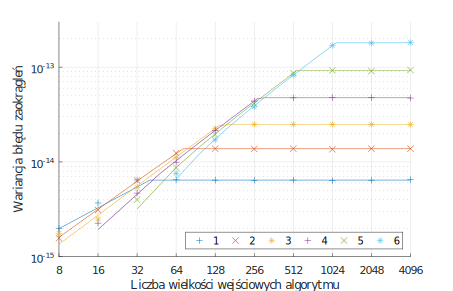
\includegraphics{obrazki/dwt_rerror_coif5}
\DIFdelbeginFL %DIFDELCMD < \makecaption{fig:dwt_rerror_coif5}{Zależność wartości wariancji sygnału błędu własnego zaokrągleń od liczby iteracji procesu dekompozycji sygnału oraz liczby wielkości wejściowych dla falki \enquote{coif5} przy stosowaniu liczb zmiennoprzecinkowych o długości słowa~\qty{32}{\bitOw}}
%DIFDELCMD < %%%
\DIFdelendFL \DIFaddbeginFL \makecaption{fig:dwt_rerror_coif5}{Zależność wartości wariancji sygnału błędu własnego zaokrągleń od liczby iteracji procesu dekompozycji sygnału oraz liczby wielkości wejściowych dla falki \enquote{coif5} przy stosowaniu liczb zmiennoprzecinkowych o długości słowa~\qty{32}{\bitOw} dla ostatniej skali detali sygnału}
\DIFaddendFL \end{center}
\end{figure}

Na podstawie rysunku~\ref{fig:dwt_rerror_coif5} zauważyć można liniowy wzrost wartości wariancji sygnału błędu zaokrągleń w funkcji liczby wielkości wejściowych, przy czym wzrost ten ustaje, gdy przestaje zwiększać się liczba operacji arytmetycznych, tj. dla takiej liczby wielkości wejściowych, która jest równa liczbie niezerowych współczynników \DIFdelbegin \DIFdel{skalujących }\DIFdelend \DIFaddbegin \DIFadd{macierzy transformacji }\DIFaddend dla analizowanego poziomu dekompozycji sygnału. W przypadku tej samej liczby wielkości wejściowych\DIFaddbegin \DIFadd{, }\DIFaddend wartość wariancji sygnału błędu zaokrągleń rośnie wraz ze wzrostem liczby iteracji procesu dekompozycji sygnału, ponieważ \DIFdelbegin \DIFdel{zwiększa się liczba niezerowych współczynników skalujących. Można zatem stwierdzić, że wartość }\DIFdelend \DIFaddbegin \DIFadd{liczba operacji arytmetycznych wzrasta dla wyższych numerów skali, co zauważyć mozna na przykładzie równań~\eqref{eq:db2_outvect_t_1_0} oraz~\eqref{eq:db2_outvect_t_2_0_rek}. Wartość }\DIFaddend wariancji błędu zaokrągleń związana jest \DIFdelbegin \DIFdel{w }\DIFdelend \DIFaddbegin \DIFadd{zatem }\DIFaddend bezpośrednio z liczbą przeprowadzanych operacji arytmetycznych \DIFdelbegin \DIFdel{, zatem }\DIFdelend \DIFaddbegin \DIFadd{i }\DIFaddend zależy od liczby współczynników skalujących oraz liczby wielkości wejściowych algorytmu.

Analizując przedstawione na rysunku~\ref{fig:dwt_rhist_coif5} histogramy realizacji sygnału błędu własnego zaokrągleń dla falki \enquote{coif5} zauważyć można, że kształt rozkładu realizacji tego sygnału jest zbliżony do kształtu rozkładu normalnego, natomiast dla poziomu ufności $\alpha = \qty{95}{\percent}$ współczynnik rozszerzenia wynosi około~\num{2.16}. Wobec powyższego, przyjęcie założenia, w którym model sygnału błędu własnego opisywany będzie rozkładem normalnym, nie jest właściwe. Aby możliwe było oszacowanie wartości współczynników koherencji zgodnie z równaniem~\eqref{eq:unc_coher}, konieczne jest wyznaczenie wartości współczynników kształtu, analogicznie jak miało to miejsce w poprzednim rozdziale. Zgodnie z równaniem~\eqref{eq:unc_shapertwo}, stosując metodę Monte-Carlo, oszacowano wartości współczynników kształtu dla sygnału błędu własnego oraz sygnałów błędów o typowych kształtach funkcji gęstości prawdopodobieństwa, a uzyskane wyniki zestawiono w tabeli~\ref{tab:unc_shapedwt}. Z uwagi na fakt, że uzyskane rozkłady sygnałów błędów własnych cechowały się bardzo zbliżonym kształtem, przedstawione wyniki stanowią uśrednione wartości dla wszystkich przeprowadzonych wcześniej eksperymentów. W dalszej cześć pracy przyjmuje się, że współczynnik kształtu oznaczony symbolem $c_{z}$ odpowiadać będzie sygnałowi błędu zaokrągleń oraz że $c_{z} = \num{2.16}$.

\begin{table}[htb!]
\begin{center}
\makecaption{tab:unc_shapedwt}{Wartości współczynników kształtu dla typowych kształtów rozkładów oraz rozkładu sygnału błędu zaokrągleń algorytmu transformacji falkowej, gdzie kolejne symbole oznaczają rozkład: (n)~normalny, (u)~jednostajny, (t)~trójkątny, (d)~dwumodalny, (r)~zaokrągleń}
\begin{tabular}[c]{| c *{5}{| S[table-format = +1.3] } |} \hline
$s_{r,*}$ & \textbf{$n$} & \textbf{$u$} & \textbf{$t$} & \textbf{$d$} & \textbf{$r$} \\ \hline
$r$       & -0.009       & 0.066        & -0.010       & 0.197        & 0.027        \\ \hline
\end{tabular}
\end{center}
\end{table}

\begin{figure}[htb!]
\begin{center}
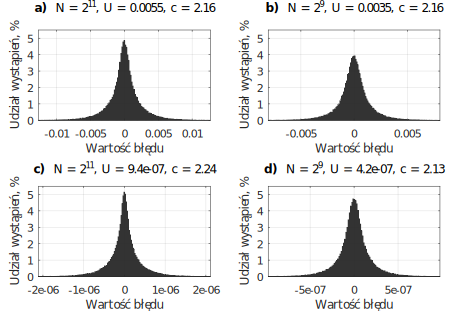
\includegraphics{obrazki/hist_numerr_coif5}
\makecaption{fig:dwt_rhist_coif5}{Histogramy realizacji sygnału błędu własnego zaokrągleń dla falki \enquote{coif5} przy sześciu iteracjach procesu dekompozycji, dla $N$ wielkości wejściowych, przy długości słowa równej \textbf{a)},~\textbf{b)}~\qty{16}{\bitOw}, \textbf{c)},~\textbf{d)}~\qty{32}{\bitOw}, przy czym niepewność rozszerzoną wyznaczono dla poziomu ufności równego \qty{95}{\percent}}
\end{center}
\end{figure}

Stosowanie liczb zmiennoprzecinkowych o długości słowa~\qty{16}{\bitOw} pozwala zmniejszyć czas obliczeń oraz rozmiar wymaganej pamięci operacyjnej w stosunku do analogicznego przypadku\DIFaddbegin \DIFadd{, }\DIFaddend wykorzystującego liczby o długości słowa~\qty{32}{\bitOw}~\cite{reay_dsp, gcc_manual}. Wariant ten wprowadza jednak znacznie większe wartości realizacji sygnałów błędów związanych z zaokrągleniami oraz większe wartości wariancji tych sygnałów ze względu na ograniczoną precyzję stosowanego zapisu liczb, co zauważyć można porównując dane zawarte w tabelach~\ref{tab:varnum_db2_2_f16} oraz~\ref{tab:varnum_db2_2_f32} dotyczące falki \enquote{db2}. W praktyce należy zatem tak dobrać długość słowa stosowanych liczb zmiennoprzecinkowych, aby wartość wariancji sygnału błędu zaokrągleń była możliwie mała w stosunku do wartości wariancji pozostałych sygnałów błędów na wyjściu algorytmu. Jeżeli przedstawione założenie zostanie spełnione, to sygnał błędu własnego algorytmu transformacji falkowej będzie mógł zostać pominięty podczas analizy właściwości toru pomiarowego~\cite{jcgm_guide}.

\DIFdelbegin %DIFDELCMD < \begin{table}[htb!]
%DIFDELCMD < \begin{center}
%DIFDELCMD < \makecaption{tab:varnum_db2_2_f16}{Zestawienie uzyskanych symulacyjnie wartości wariancji sygnału błędu zaokrągleń kolejnych wielkości wyjściowych algorytmu dyskretnej transformacji falkowej dla falki \enquote{db2} przy dwóch iteracjach procesu dekompozycji, dla liczb o długości~\qty{16}{\bitOw}, w zależności od zakresu możliwych wartości realizacji wielkości wejściowych}
%DIFDELCMD < \begin{tabular}[c]{| c *{6}{|S[table-format = 1.2e+1, mode = math]} |} \hline
%DIFDELCMD < \multirow{2}{*}{$X$} & \multicolumn{6}{ c |}{\textbf{Zakres wielkości wejściowych algorytmu}} \\ \cline{2-7}
%DIFDELCMD < & \text{$<-1;1>$} & \text{$<-2;2>$} & \text{$<-3;3>$} & \text{$<0;2>$} & \text{$<0;4>$} & \text{$<3;9>$} \\ \hline
%DIFDELCMD < $S_{2,0}$ & 1.03e-7 & 4.12e-7 & 9.74e-7 & 7.08e-7 & 2.83e-6 & 2.16e-5 \\ \hline
%DIFDELCMD < $S_{2,1}$ & 1.11e-7 & 4.43e-7 & 1.01e-6 & 9.55e-7 & 3.82e-6 & 2.75e-5 \\ \hline
%DIFDELCMD < $T_{2,0}$ & 1.31e-7 & 5.24e-7 & 1.21e-6 & 2.87e-7 & 1.15e-6 & 7.06e-6 \\ \hline
%DIFDELCMD < $T_{2,1}$ & 1.07e-7 & 4.29e-7 & 9.73e-7 & 3.36e-7 & 1.34e-6 & 9.30e-6 \\ \hline
%DIFDELCMD < $T_{1,0}$ & 7.09e-8 & 2.85e-7 & 6.99e-7 & 1.65e-7 & 3.56e-7 & 4.29e-6 \\ \hline
%DIFDELCMD < $T_{1,1}$ & 5.83e-8 & 2.33e-7 & 5.87e-7 & 1.49e-7 & 5.95e-7 & 4.05e-6 \\ \hline
%DIFDELCMD < $T_{1,2}$ & 5.84e-8 & 2.34e-7 & 5.85e-7 & 1.49e-7 & 5.97e-7 & 4.05e-6 \\ \hline
%DIFDELCMD < $T_{1,3}$ & 5.53e-8 & 2.21e-7 & 5.41e-7 & 1.78e-7 & 7.08e-7 & 5.26e-6 \\ \hline
%DIFDELCMD < \end{tabular}
%DIFDELCMD < \end{center}
%DIFDELCMD < \end{table}
%DIFDELCMD < %%%
\DIFdelend \DIFaddbegin \begin{table}[htb!]
\begin{center}
\makecaption{tab:varnum_db2_2_f16}{Zestawienie uzyskanych symulacyjnie wartości wariancji sygnału błędu zaokrągleń kolejnych wielkości wyjściowych algorytmu dyskretnej transformacji falkowej dla falki \enquote{db2} przy dwóch iteracjach procesu dekompozycji, dla liczb o długości~\qty{16}{\bitOw}, w zależności od zakresu możliwych wartości realizacji wielkości wejściowych}
\begin{tabular}[c]{| c *{6}{|S[table-format = 1.2e+1, mode = math]} |} \hline
\multirow{2}{*}{$X$} & \multicolumn{6}{ c |}{\textbf{Zakres wartości realizacji wielkości wejściowych algorytmu}} \\ \cline{2-7}
& $\interval{-1}{1}$ & $\interval{-2}{2}$ & $\interval{-3}{3}$ & $\interval{0}{2}$ & $\interval{0}{4}$ & $\interval{3}{9}$ \\ \hline
$S_{2,0}$ & 1.03e-7 & 4.12e-7 & 9.74e-7 & 7.08e-7 & 2.83e-6 & 2.16e-5 \\ \hline
$S_{2,1}$ & 1.11e-7 & 4.43e-7 & 1.01e-6 & 9.55e-7 & 3.82e-6 & 2.75e-5 \\ \hline
$T_{2,0}$ & 1.31e-7 & 5.24e-7 & 1.21e-6 & 2.87e-7 & 1.15e-6 & 7.06e-6 \\ \hline
$T_{2,1}$ & 1.07e-7 & 4.29e-7 & 9.73e-7 & 3.36e-7 & 1.34e-6 & 9.30e-6 \\ \hline
$T_{1,0}$ & 7.09e-8 & 2.85e-7 & 6.99e-7 & 1.65e-7 & 3.56e-7 & 4.29e-6 \\ \hline
$T_{1,1}$ & 5.83e-8 & 2.33e-7 & 5.87e-7 & 1.49e-7 & 5.95e-7 & 4.05e-6 \\ \hline
$T_{1,2}$ & 5.84e-8 & 2.34e-7 & 5.85e-7 & 1.49e-7 & 5.97e-7 & 4.05e-6 \\ \hline
$T_{1,3}$ & 5.53e-8 & 2.21e-7 & 5.41e-7 & 1.78e-7 & 7.08e-7 & 5.26e-6 \\ \hline
\end{tabular}
\end{center}
\end{table}
\DIFaddend 

\DIFdelbegin %DIFDELCMD < \begin{table}[htb!]
%DIFDELCMD < \begin{center}
%DIFDELCMD < \makecaption{tab:varnum_db2_2_f32}{Zestawienie uzyskanych symulacyjnie wartości wariancji sygnału błędu zaokrągleń kolejnych wielkości wyjściowych algorytmu dyskretnej transformacji falkowej dla falki \enquote{db2} przy dwóch iteracjach procesu dekompozycji, dla liczb o długości~\qty{32}{\bitOw}, w zależności od zakresu możliwych wartości realizacji wielkości wejściowych}
%DIFDELCMD < \begin{tabular}[c]{| c *{6}{|S[table-format = 1.2e+2, mode = math]} |} \hline
%DIFDELCMD < \multirow{2}{*}{$X$} & \multicolumn{6}{ c |}{\textbf{Zakres wielkości wejściowych algorytmu}} \\ \cline{2-7}
%DIFDELCMD < & \text{$<-1;1>$} & \text{$<-2;2>$} & \text{$<-3;3>$} & \text{$<0;2>$} & \text{$<0;4>$} & \text{$<3;9>$} \\ \hline
%DIFDELCMD < $S_{2,0}$ & 1.40e-15 & 5.57e-15 & 1.30e-14 & 9.29e-15 & 3.71e-14 & 2.78e-13 \\ \hline
%DIFDELCMD < $S_{2,1}$ & 1.40e-15 & 5.61e-15 & 1.29e-14 & 1.25e-14 & 5.00e-14 & 3.54e-13 \\ \hline
%DIFDELCMD < $T_{2,0}$ & 1.71e-15 & 6.83e-15 & 1.58e-14 & 3.33e-15 & 1.33e-14 & 7.78e-14 \\ \hline
%DIFDELCMD < $T_{2,1}$ & 1.39e-15 & 5.56e-15 & 1.29e-14 & 4.27e-15 & 1.71e-14 & 1.16e-13 \\ \hline
%DIFDELCMD < $T_{1,0}$ & 8.28e-16 & 3.54e-15 & 8.38e-15 & 1.70e-15 & 6.84e-15 & 4.25e-14 \\ \hline
%DIFDELCMD < $T_{1,1}$ & 6.82e-16 & 2.72e-15 & 6.67e-15 & 1.46e-15 & 5.84e-15 & 4.02e-14 \\ \hline
%DIFDELCMD < $T_{1,2}$ & 6.82e-16 & 2.72e-15 & 6.66e-15 & 1.47e-15 & 5.86e-15 & 4.02e-14 \\ \hline
%DIFDELCMD < $T_{1,3}$ & 6.68e-16 & 2.67e-15 & 6.48e-15 & 2.02e-15 & 8.10e-15 & 6.15e-14 \\ \hline
%DIFDELCMD < \end{tabular}
%DIFDELCMD < \end{center}
%DIFDELCMD < \end{table}
%DIFDELCMD < %%%
\DIFdelend \DIFaddbegin \begin{table}[htb!]
\begin{center}
\makecaption{tab:varnum_db2_2_f32}{Zestawienie uzyskanych symulacyjnie wartości wariancji sygnału błędu zaokrągleń kolejnych wielkości wyjściowych algorytmu dyskretnej transformacji falkowej dla falki \enquote{db2} przy dwóch iteracjach procesu dekompozycji, dla liczb o długości~\qty{32}{\bitOw}, w zależności od zakresu możliwych wartości realizacji wielkości wejściowych}
\begin{tabular}[c]{| c *{6}{|S[table-format = 1.2e+2, mode = math]} |} \hline
\multirow{2}{*}{$X$} & \multicolumn{6}{ c |}{\textbf{Zakres wartości realizacji wielkości wejściowych algorytmu}} \\ \cline{2-7}
& $\interval{-1}{1}$ & $\interval{-2}{2}$ & $\interval{-3}{3}$ & $\interval{0}{2}$ & $\interval{0}{4}$ & $\interval{3}{9}$ \\ \hline
$S_{2,0}$ & 1.40e-15 & 5.57e-15 & 1.30e-14 & 9.29e-15 & 3.71e-14 & 2.78e-13 \\ \hline
$S_{2,1}$ & 1.40e-15 & 5.61e-15 & 1.29e-14 & 1.25e-14 & 5.00e-14 & 3.54e-13 \\ \hline
$T_{2,0}$ & 1.71e-15 & 6.83e-15 & 1.58e-14 & 3.33e-15 & 1.33e-14 & 7.78e-14 \\ \hline
$T_{2,1}$ & 1.39e-15 & 5.56e-15 & 1.29e-14 & 4.27e-15 & 1.71e-14 & 1.16e-13 \\ \hline
$T_{1,0}$ & 8.28e-16 & 3.54e-15 & 8.38e-15 & 1.70e-15 & 6.84e-15 & 4.25e-14 \\ \hline
$T_{1,1}$ & 6.82e-16 & 2.72e-15 & 6.67e-15 & 1.46e-15 & 5.84e-15 & 4.02e-14 \\ \hline
$T_{1,2}$ & 6.82e-16 & 2.72e-15 & 6.66e-15 & 1.47e-15 & 5.86e-15 & 4.02e-14 \\ \hline
$T_{1,3}$ & 6.68e-16 & 2.67e-15 & 6.48e-15 & 2.02e-15 & 8.10e-15 & 6.15e-14 \\ \hline
\end{tabular}
\end{center}
\end{table}
\DIFaddend 

Jako, że zakres możliwych wartości realizacji wielkości wejściowych algorytmu transformacji falkowej również wpływa na wprowadzane błędy zaokrągleń, należy brać ten czynnik pod uwagę podczas analizy projektowanego toru pomiarowego. Podobna zależność występuje również dla kształtu rozkładu realizacji omawianego sygnału. Należy zatem tak dobrać warunki eksperymentu mającego na celu identyfikacje parametrów sygnału błędu własnego, aby w jak największym stopniu były one zbieżne z warunkami rzeczywistymi. Analizując wyniki eksperymentu zauważyć można, że wraz ze wzrostem zakresu wartości wielkości wejściowych wartość wariancji sygnału błędu zaokrągleń wzrasta. Zależność ta wynika bezpośrednio z właściwości stosowanej metody zapisu liczb zmiennoprzecinkowych i została szerzej opisana w publikacji~\cite{benz_floats}.

\DIFdelbegin %DIFDELCMD < \begin{table}[htb!]
%DIFDELCMD < \begin{center}
%DIFDELCMD < \makecaption{tab:varnum_db2_5_f16}{Zestawienie uzyskanych symulacyjnie wartości wariancji sygnału błędu zaokrągleń kolejnych grup wielkości wyjściowych algorytmu dyskretnej transformacji falkowej dla falki \enquote{db2} przy pięciu iteracjach procesu dekompozycji, dla liczb o długości~\qty{16}{\bitOw}, w zależności od zakresu możliwych wartości realizacji wielkości wejściowych}
%DIFDELCMD < \begin{tabular}[c]{| c *{6}{|S[table-format = 1.2e+1, mode = math]} |} \hline
%DIFDELCMD < \multirow{2}{*}{$N$} & \multicolumn{6}{ c |}{\textbf{Skala wielkości wyjściowych algorytmu}} \\ \cline{2-7}
%DIFDELCMD < & \text{$S_5$} & \text{$T_5$} & \text{$T_4$} & \text{$T_3$} & \text{$T_2$} & \text{$T_1$} \\ \hline
%DIFDELCMD < \textbf{64}   & 4.91e-7 & 5.31e-7 & 3.94e-7 & 2.09e-7 & 1.23e-7 & 5.86e-8 \\ \hline
%DIFDELCMD < \textbf{128}  & 7.51e-7 & 7.08e-7 & 3.87e-7 & 2.07e-7 & 1.22e-7 & 5.85e-8 \\ \hline
%DIFDELCMD < \textbf{256}  & 8.59e-7 & 6.99e-7 & 3.85e-7 & 2.05e-7 & 1.21e-7 & 5.84e-8 \\ \hline
%DIFDELCMD < \textbf{512}  & 9.19e-7 & 6.89e-7 & 3.81e-7 & 2.04e-7 & 1.21e-7 & 5.84e-8 \\ \hline
%DIFDELCMD < \textbf{1024} & 9.47e-7 & 6.85e-7 & 3.80e-7 & 2.04e-7 & 1.21e-7 & 5.84e-8 \\ \hline
%DIFDELCMD < \textbf{2048} & 9.58e-7 & 6.84e-7 & 3.80e-7 & 2.04e-7 & 1.21e-7 & 5.84e-8 \\ \hline
%DIFDELCMD < \textbf{4096} & 9.66e-7 & 6.83e-7 & 3.80e-7 & 2.04e-7 & 1.21e-7 & 5.84e-8 \\ \hline
%DIFDELCMD < \end{tabular}
%DIFDELCMD < \end{center}
%DIFDELCMD < \end{table}
%DIFDELCMD < %%%
\DIFdelend \DIFaddbegin \begin{table}[htb!]
\begin{center}
\makecaption{tab:varnum_db2_5_f16}{Zestawienie uzyskanych symulacyjnie wartości wariancji sygnału błędu zaokrągleń kolejnych grup wielkości wyjściowych algorytmu dyskretnej transformacji falkowej dla falki \enquote{db2} przy pięciu iteracjach procesu dekompozycji, dla liczb o długości~\qty{16}{\bitOw}, w zależności od liczby wielkości wejściowych algorytmu}
\begin{tabular}[c]{| c *{6}{|S[table-format = 1.2e+1, mode = math]} |} \hline
\multirow{2}{*}{$N$} & \multicolumn{6}{ c |}{\textbf{Skala wielkości wyjściowych algorytmu}} \\ \cline{2-7}
& \text{$S_5$} & \text{$T_5$} & \text{$T_4$} & \text{$T_3$} & \text{$T_2$} & \text{$T_1$} \\ \hline
\textbf{64}   & 4.91e-7 & 5.31e-7 & 3.94e-7 & 2.09e-7 & 1.23e-7 & 5.86e-8 \\ \hline
\textbf{128}  & 7.51e-7 & 7.08e-7 & 3.87e-7 & 2.07e-7 & 1.22e-7 & 5.85e-8 \\ \hline
\textbf{256}  & 8.59e-7 & 6.99e-7 & 3.85e-7 & 2.05e-7 & 1.21e-7 & 5.84e-8 \\ \hline
\textbf{512}  & 9.19e-7 & 6.89e-7 & 3.81e-7 & 2.04e-7 & 1.21e-7 & 5.84e-8 \\ \hline
\textbf{1024} & 9.47e-7 & 6.85e-7 & 3.80e-7 & 2.04e-7 & 1.21e-7 & 5.84e-8 \\ \hline
\textbf{2048} & 9.58e-7 & 6.84e-7 & 3.80e-7 & 2.04e-7 & 1.21e-7 & 5.84e-8 \\ \hline
\textbf{4096} & 9.66e-7 & 6.83e-7 & 3.80e-7 & 2.04e-7 & 1.21e-7 & 5.84e-8 \\ \hline
\end{tabular}
\end{center}
\end{table}
\DIFaddend 

\DIFdelbegin %DIFDELCMD < \begin{table}[htb!]
%DIFDELCMD < \begin{center}
%DIFDELCMD < \makecaption{tab:varnum_db2_5_f32}{Zestawienie uzyskanych symulacyjnie wartości wariancji sygnału błędu zaokrągleń kolejnych grup wielkości wyjściowych algorytmu dyskretnej transformacji falkowej dla falki \enquote{db2} przy pięciu iteracjach procesu dekompozycji, dla liczb o długości~\qty{32}{\bitOw}, w zależności od zakresu możliwych wartości realizacji wielkości wejściowych}
%DIFDELCMD < \begin{tabular}[c]{| c *{6}{|S[table-format = 1.2e+2, mode = math]} |} \hline
%DIFDELCMD < \multirow{2}{*}{$N$} & \multicolumn{6}{ c |}{\textbf{Skala wielkości wyjściowych algorytmu}} \\ \cline{2-7}
%DIFDELCMD < & \text{$S_5$} & \text{$T_5$} & \text{$T_4$} & \text{$T_3$} & \text{$T_2$} & \text{$T_1$} \\ \hline
%DIFDELCMD < \textbf{64}   & 6.83e-15 & 7.93e-15 & 5.42e-15 & 2.86e-15 & 1.62e-15 & 7.12e-16 \\ \hline
%DIFDELCMD < \textbf{128}  & 1.15e-14 & 1.02e-14 & 5.39e-15 & 2.79e-15 & 1.58e-15 & 6.98e-16 \\ \hline
%DIFDELCMD < \textbf{256}  & 1.34e-14 & 1.03e-14 & 5.30e-15 & 2.76e-15 & 1.56e-15 & 6.90e-16 \\ \hline
%DIFDELCMD < \textbf{512}  & 1.44e-14 & 1.03e-14 & 5.25e-15 & 2.73e-15 & 1.55e-15 & 6.85e-16 \\ \hline
%DIFDELCMD < \textbf{1024} & 1.49e-14 & 1.03e-14 & 5.23e-15 & 2.72e-15 & 1.55e-15 & 6.84e-16 \\ \hline
%DIFDELCMD < \textbf{2048} & 1.51e-14 & 1.03e-14 & 5.22e-15 & 2.72e-15 & 1.55e-15 & 6.84e-16 \\ \hline
%DIFDELCMD < \textbf{4096} & 1.52e-14 & 1.03e-14 & 5.22e-15 & 2.72e-15 & 1.55e-15 & 6.84e-16 \\ \hline
%DIFDELCMD < \end{tabular}
%DIFDELCMD < \end{center}
%DIFDELCMD < \end{table}
%DIFDELCMD < %%%
\DIFdelend \DIFaddbegin \begin{table}[htb!]
\begin{center}
\makecaption{tab:varnum_db2_5_f32}{Zestawienie uzyskanych symulacyjnie wartości wariancji sygnału błędu zaokrągleń kolejnych grup wielkości wyjściowych algorytmu dyskretnej transformacji falkowej dla falki \enquote{db2} przy pięciu iteracjach procesu dekompozycji, dla liczb o długości~\qty{32}{\bitOw}, w zależności od liczby wielkości wejściowych algorytmu}
\begin{tabular}[c]{| c *{6}{|S[table-format = 1.2e+2, mode = math]} |} \hline
\multirow{2}{*}{$N$} & \multicolumn{6}{ c |}{\textbf{Skala wielkości wyjściowych algorytmu}} \\ \cline{2-7}
& \text{$S_5$} & \text{$T_5$} & \text{$T_4$} & \text{$T_3$} & \text{$T_2$} & \text{$T_1$} \\ \hline
\textbf{64}   & 6.83e-15 & 7.93e-15 & 5.42e-15 & 2.86e-15 & 1.62e-15 & 7.12e-16 \\ \hline
\textbf{128}  & 1.15e-14 & 1.02e-14 & 5.39e-15 & 2.79e-15 & 1.58e-15 & 6.98e-16 \\ \hline
\textbf{256}  & 1.34e-14 & 1.03e-14 & 5.30e-15 & 2.76e-15 & 1.56e-15 & 6.90e-16 \\ \hline
\textbf{512}  & 1.44e-14 & 1.03e-14 & 5.25e-15 & 2.73e-15 & 1.55e-15 & 6.85e-16 \\ \hline
\textbf{1024} & 1.49e-14 & 1.03e-14 & 5.23e-15 & 2.72e-15 & 1.55e-15 & 6.84e-16 \\ \hline
\textbf{2048} & 1.51e-14 & 1.03e-14 & 5.22e-15 & 2.72e-15 & 1.55e-15 & 6.84e-16 \\ \hline
\textbf{4096} & 1.52e-14 & 1.03e-14 & 5.22e-15 & 2.72e-15 & 1.55e-15 & 6.84e-16 \\ \hline
\end{tabular}
\end{center}
\end{table}
\DIFaddend 

\DIFdelbegin %DIFDELCMD < \begin{table}[htb!]
%DIFDELCMD < \begin{center}
%DIFDELCMD < \makecaption{tab:varnum_spline4_4_5_f16}{Zestawienie uzyskanych symulacyjnie wartości wariancji sygnału błędu zaokrągleń kolejnych grup wielkości wyjściowych algorytmu dyskretnej transformacji falkowej dla falki \enquote{spline2:4} przy pięciu iteracjach procesu dekompozycji, dla liczb o długości~\qty{16}{\bitOw}, w zależności od zakresu możliwych wartości realizacji wielkości wejściowych}
%DIFDELCMD < \begin{tabular}[c]{| c *{6}{|S[table-format = 1.2e+1, mode = math]} |} \hline
%DIFDELCMD < \multirow{2}{*}{$N$} & \multicolumn{6}{ c |}{\textbf{Skala wielkości wyjściowych algorytmu}} \\ \cline{2-7}
%DIFDELCMD < & \text{$S_5$} & \text{$T_5$} & \text{$T_4$} & \text{$T_3$} & \text{$T_2$} & \text{$T_1$} \\ \hline
%DIFDELCMD < \textbf{64}   & 1.07e-6 & 1.02e-6 & 8.94e-7 & 5.05e-7 & 1.83e-7 & 4.76e-8 \\ \hline
%DIFDELCMD < \textbf{128}  & 1.75e-6 & 1.59e-6 & 9.22e-7 & 4.96e-7 & 1.80e-7 & 4.64e-8 \\ \hline
%DIFDELCMD < \textbf{256}  & 2.61e-6 & 1.67e-6 & 9.11e-7 & 4.91e-7 & 1.77e-7 & 4.58e-8 \\ \hline
%DIFDELCMD < \textbf{512}  & 2.60e-6 & 1.69e-6 & 9.05e-7 & 4.89e-7 & 1.76e-7 & 4.55e-8 \\ \hline
%DIFDELCMD < \textbf{1024} & 2.58e-6 & 1.71e-6 & 9.02e-7 & 4.88e-7 & 1.75e-7 & 4.53e-8 \\ \hline
%DIFDELCMD < \textbf{2048} & 2.58e-6 & 1.71e-6 & 9.00e-7 & 4.87e-7 & 1.75e-7 & 4.53e-8 \\ \hline
%DIFDELCMD < \textbf{4096} & 2.58e-6 & 1.72e-6 & 9.00e-7 & 4.87e-7 & 1.75e-7 & 4.53e-8 \\ \hline
%DIFDELCMD < \end{tabular}
%DIFDELCMD < \end{center}
%DIFDELCMD < \end{table}
%DIFDELCMD < %%%
\DIFdelend \DIFaddbegin \begin{table}[htb!]
\begin{center}
\makecaption{tab:varnum_spline4_4_5_f16}{Zestawienie uzyskanych symulacyjnie wartości wariancji sygnału błędu zaokrągleń kolejnych grup wielkości wyjściowych algorytmu dyskretnej transformacji falkowej dla falki \enquote{spline2:4} przy pięciu iteracjach procesu dekompozycji, dla liczb o długości~\qty{16}{\bitOw}, w zależności od liczby wielkości wejściowych algorytmu}
\begin{tabular}[c]{| c *{6}{|S[table-format = 1.2e+1, mode = math]} |} \hline
\multirow{2}{*}{$N$} & \multicolumn{6}{ c |}{\textbf{Skala wielkości wyjściowych algorytmu}} \\ \cline{2-7}
& \text{$S_5$} & \text{$T_5$} & \text{$T_4$} & \text{$T_3$} & \text{$T_2$} & \text{$T_1$} \\ \hline
\textbf{64}   & 1.07e-6 & 1.02e-6 & 8.94e-7 & 5.05e-7 & 1.83e-7 & 4.76e-8 \\ \hline
\textbf{128}  & 1.75e-6 & 1.59e-6 & 9.22e-7 & 4.96e-7 & 1.80e-7 & 4.64e-8 \\ \hline
\textbf{256}  & 2.61e-6 & 1.67e-6 & 9.11e-7 & 4.91e-7 & 1.77e-7 & 4.58e-8 \\ \hline
\textbf{512}  & 2.60e-6 & 1.69e-6 & 9.05e-7 & 4.89e-7 & 1.76e-7 & 4.55e-8 \\ \hline
\textbf{1024} & 2.58e-6 & 1.71e-6 & 9.02e-7 & 4.88e-7 & 1.75e-7 & 4.53e-8 \\ \hline
\textbf{2048} & 2.58e-6 & 1.71e-6 & 9.00e-7 & 4.87e-7 & 1.75e-7 & 4.53e-8 \\ \hline
\textbf{4096} & 2.58e-6 & 1.72e-6 & 9.00e-7 & 4.87e-7 & 1.75e-7 & 4.53e-8 \\ \hline
\end{tabular}
\end{center}
\end{table}
\DIFaddend 

\DIFdelbegin %DIFDELCMD < \begin{table}[htb!]
%DIFDELCMD < \begin{center}
%DIFDELCMD < \makecaption{tab:varnum_spline4_4_5_f32}{Zestawienie uzyskanych symulacyjnie wartości wariancji sygnału błędu zaokrągleń kolejnych grup wielkości wyjściowych algorytmu dyskretnej transformacji falkowej dla falki \enquote{spline2:4} przy pięciu iteracjach procesu dekompozycji, dla liczb o długości~\qty{32}{\bitOw}, w zależności od zakresu możliwych wartości realizacji wielkości wejściowych}
%DIFDELCMD < \begin{tabular}[c]{| c *{6}{|S[table-format = 1.2e+2, mode = math]} |} \hline
%DIFDELCMD < \multirow{2}{*}{$N$} & \multicolumn{6}{ c |}{\textbf{Skala wielkości wyjściowych algorytmu}} \\ \cline{2-7}
%DIFDELCMD < & \text{$S_5$} & \text{$T_5$} & \text{$T_4$} & \text{$T_3$} & \text{$T_2$} & \text{$T_1$} \\ \hline
%DIFDELCMD < \textbf{64}   & 1.51e-14 & 1.44e-14 & 1.26e-14 & 6.54e-15 & 2.33e-15 & 5.44e-16 \\ \hline
%DIFDELCMD < \textbf{128}  & 2.52e-14 & 2.37e-14 & 1.45e-14 & 6.50e-15 & 2.27e-15 & 5.29e-16 \\ \hline
%DIFDELCMD < \textbf{256}  & 4.72e-14 & 2.91e-14 & 1.45e-14 & 6.40e-15 & 2.24e-15 & 5.22e-16 \\ \hline
%DIFDELCMD < \textbf{512}  & 4.72e-14 & 2.98e-14 & 1.44e-14 & 6.36e-15 & 2.23e-15 & 5.17e-16 \\ \hline
%DIFDELCMD < \textbf{1024} & 4.71e-14 & 3.01e-14 & 1.43e-14 & 6.35e-15 & 2.22e-15 & 5.16e-16 \\ \hline
%DIFDELCMD < \textbf{2048} & 4.72e-14 & 3.03e-14 & 1.43e-14 & 6.35e-15 & 2.22e-15 & 5.16e-16 \\ \hline
%DIFDELCMD < \textbf{4096} & 4.72e-14 & 3.04e-14 & 1.43e-14 & 6.35e-15 & 2.22e-15 & 5.16e-16 \\ \hline
%DIFDELCMD < \end{tabular}
%DIFDELCMD < \end{center}
%DIFDELCMD < \end{table}
%DIFDELCMD < %%%
\DIFdelend \DIFaddbegin \begin{table}[htb!]
\begin{center}
\makecaption{tab:varnum_spline4_4_5_f32}{Zestawienie uzyskanych symulacyjnie wartości wariancji sygnału błędu zaokrągleń kolejnych grup wielkości wyjściowych algorytmu dyskretnej transformacji falkowej dla falki \enquote{spline2:4} przy pięciu iteracjach procesu dekompozycji, dla liczb o długości~\qty{32}{\bitOw}, w zależności od liczby wielkości wejściowych algorytmu}
\begin{tabular}[c]{| c *{6}{|S[table-format = 1.2e+2, mode = math]} |} \hline
\multirow{2}{*}{$N$} & \multicolumn{6}{ c |}{\textbf{Skala wielkości wyjściowych algorytmu}} \\ \cline{2-7}
& \text{$S_5$} & \text{$T_5$} & \text{$T_4$} & \text{$T_3$} & \text{$T_2$} & \text{$T_1$} \\ \hline
\textbf{64}   & 1.51e-14 & 1.44e-14 & 1.26e-14 & 6.54e-15 & 2.33e-15 & 5.44e-16 \\ \hline
\textbf{128}  & 2.52e-14 & 2.37e-14 & 1.45e-14 & 6.50e-15 & 2.27e-15 & 5.29e-16 \\ \hline
\textbf{256}  & 4.72e-14 & 2.91e-14 & 1.45e-14 & 6.40e-15 & 2.24e-15 & 5.22e-16 \\ \hline
\textbf{512}  & 4.72e-14 & 2.98e-14 & 1.44e-14 & 6.36e-15 & 2.23e-15 & 5.17e-16 \\ \hline
\textbf{1024} & 4.71e-14 & 3.01e-14 & 1.43e-14 & 6.35e-15 & 2.22e-15 & 5.16e-16 \\ \hline
\textbf{2048} & 4.72e-14 & 3.03e-14 & 1.43e-14 & 6.35e-15 & 2.22e-15 & 5.16e-16 \\ \hline
\textbf{4096} & 4.72e-14 & 3.04e-14 & 1.43e-14 & 6.35e-15 & 2.22e-15 & 5.16e-16 \\ \hline
\end{tabular}
\end{center}
\end{table}
\DIFaddend 

\section{Implementacja okna pomiarowego}

Identycznie, jak w przypadku innych algorytmów przetwarzających ciągi wielkości wejściowych, dla algorytmu transformacji falkowej stosować można wybrane okno pomiarowe. Wprowadzenie okna pomiarowego\DIFdelbegin \DIFdel{oznaczonego jako }\DIFdelend \DIFaddbegin \DIFadd{, którego funkcję oznaczono symbolem }\DIFaddend $w(n)$\DIFaddbegin \DIFadd{, }\DIFaddend można przedstawić za pomocą modyfikacji równania~\eqref{eq:alg_out_single}\DIFdelbegin \DIFdel{jako}\DIFdelend :
\begin{equation}
X \emb{i} = a_{i, 0} w \emb{0} x \emb{0} + a_{i, 1} w \emb{1} x \emb{1} + \hdots + a_{i, N-1} w \emb{N-1} x \emb{N-1} \label{eq:wt_singlewindow}.
\end{equation}
Na podstawie przedstawionego równania zauważyć można, że wprowadzenie okna pomiarowego opisać można również za pomocą modyfikacji współczynników macierzy transformacji algorytmu zgodnie z zależnością opisaną równaniem:
\begin{equation}
a'_{i,j} = w \emb{j} a_{i,j} \label{eq:wt_windowmod},
\end{equation}
gdzie $a'_{i,j}$ stanowi nową wartość współczynnika macierzy transformacji algorytmu. Użyta funkcja $w(n)$ powinna być opisana dla wartości $n$ w przedziale \DIFdelbegin \DIFdel{$<0;N-1>$}\DIFdelend \DIFaddbegin \DIFadd{$\interval{0}{N-1}$}\DIFaddend . Należy zaznaczyć, że stosowanie okna pomiarowego spowoduje zmianę transmitancji związanych z kolejnymi wielkościami wyjściowymi algorytmu, a zatem będzie miało wpływ na widmo sygnałów wielkości wyjściowych.

Wybrane okna pomiarowe opisane w literaturze~\cite{oppenheim_dsp, oppenheim_sns, proakis_dsp} to okna: trójkątne~\eqref{eq:wnd_triang}, sinusoidalne~\eqref{eq:wnd_sine}, Gaussa~\eqref{eq:wnd_gauss}, Hamminga~\eqref{eq:wnd_hamming}, Hanna~\eqref{eq:wnd_hann} oraz Welcha~\eqref{eq:wnd_welch}, które opisać można kolejno w postaci:
\begin{gather}
w_{tr} \emb{n} = 1 - \left| \frac{n - \frac{N-1}{2}}{\frac{N}{2}} \right| \label{eq:wnd_triang}, \\
w_{sn} \emb{n} = \sin \left( \frac{\pi n}{N} \right) \label{eq:wnd_sine}, \\
w_{ga} \emb{n} = \exp \left(-\frac{1}{2} \left( \frac{n - \frac{N-1}{2}}{\sigma \frac{\emb{N-1}}{2}} \right)^{2} \right) \label{eq:wnd_gauss}, \\
w_{hm} \emb{n} = \num{0.5384} - \num{0.4616} \cos \left( \frac{2 \pi n}{N} \right) \label{eq:wnd_hamming}, \\
w_{hn} \emb{n} = \num{0.5} \left(1 - \cos \left( \frac{2 \pi n}{N} \right) \right) \label{eq:wnd_hann}, \\
w_{wh} \emb{n} = 1 - \left( \frac{n - \frac{N}{2}}{\frac{N}{2}} \right)^{2} \label{eq:wnd_welch}.
\end{gather}
W dalszej części pracy stosuje się okno prostokątne, w którym $w(n) = 1$, o ile nie został zaznaczony fakt stosowania innego okna pomiarowego.

Implementacja okna pomiarowego, z punktu widzenia przedstawionych w pracy założeń, mogłaby również zostać opisana jako zastosowanie dodatkowego algorytmu. Algorytm ten przetwarzałby $N$ wielkości wejściowych na $M$ wielkości wyjściowych, gdzie $N = M$. Macierz transformacji omawianego algorytmu byłaby macierzą diagonalną, przy czym wartości kolejnych współczynników odpowiadałyby wyznaczonym wagom dla $i$-tej wielkości okna. Z praktycznego punktu widzenia zaproponowana metoda modyfikacji wartości współczynników transformacji algorytmu transformacji falkowej wydaje się jednak bardziej korzystna. Na tej samej zasadzie istnieje możliwość implementacji innych modyfikacji, np. wprowadzenia dodatkowego filtru. Jako, że algorytm dyskretnej transformacji sam w sobie implementuje dla kolejnych wielkości wyjściowych podział tych wielkości na odpowiadające im okna pomiarowe, stosowanie dodatkowego okna pomiarowego nie jest tak popularne, jak w przypadku innych algorytmów (np. algorytmu \enquote{DFT}). Zagadnienie to nie zostało zatem poruszone szczegółowo w pracy.

Jako, że wprowadzenie okna pomiarowego skutkuje zmianą wypadkowej transmitancji związanej z wielkościami wyjściowymi algorytmu, działanie to wpływa na przenoszone z wejścia na wyjście algorytmu sygnały błędów. Aplikację omawianej metody oraz wpływ parametrów okna pomiarowego na przenoszenie błędów losowych przez algorytmy dyskretnej transformacji falkowej opisano w pracy~\cite{auth_window}. Należy zauważyć, że w omawianym przypadku każda z wielkości wyjściowych cechować się będzie inną transmitancją, a zatem przeprowadzenie zbiorczej analizy dla wielkości wyjściowych związanych z tym samym poziomem dekompozycji jest niemożliwe.

\section{Podsumowanie rozdziału}

Specyfika algorytmów transformacji falkowej pozwala na analizę właściwości metrologicznych tych algorytmów stosując model błędów opisany w pracy dla cyfrowej cześć toru pomiarowego. W ogólnym przypadku algorytm transformacji falkowej traktować można jako zbiór $K+1$ filtrów, gdzie $K$ jest liczbą iteracji procesu dekompozycji sygnału. Transmitancja algorytmu\DIFaddbegin \DIFadd{, }\DIFaddend odpowiednia dla kolejnych wielkości wyjściowych związanych z tą samą iteracją procesu dekompozycji sygnału\DIFaddbegin \DIFadd{, }\DIFaddend jest identyczna, natomiast na wejście filtru podawane są różne numery próbek wielkości wejściowych poprzedniego etapu dekompozycji, co związane jest z przesunięciem okna pomiarowego. Transmitancja algorytmu może być określana na podstawie znajomości wartości współczynników skalujących, stosowanych również w celu wyznaczania wartości współczynników macierzy transformacji tego algorytmu. Należy zaznaczyć, że w pewnych przypadkach transmitancja algorytmu związana z kolejnymi wielkościami wyjściowymi może być różna (np. jeżeli stosowane jest okno pomiarowe).

Jak zaznaczono we wstępnie do pracy, wszystkie przedstawione informacje dotyczące algorytmów transformacji falkowej stanowią podsumowanie zawartych w literaturze rozważań. Dorobek autora pracy stanowi natomiast wskazanie istotnych, z punktu widzenia analizy właściwości metrologicznych torów pomiarowych, cech tych algorytmów, a także zaproponowanie jednolitej metody opisu miary niedokładności wyznaczania wartości realizacji ich wielkości wyjściowych. Zaproponowane w pracy podejście do analizy właściwości metrologicznych algorytmów transformacji falkowej oraz wskazanie roli tych algorytmów w procesie propagacji sygnałów błędów ich wielkości wejściowych nie było dotychczas przedstawione w literaturze. Stosowanie proponowanej metody możliwe jest dla dowolnych parametrów algorytmu transformacji falkowej o wielkościach wejściowych z dziedziny liczb rzeczywistych. Istotnym walorem pracy, zawartym w bieżącym rozdziale, jest również wskazanie sposobu aplikacji zaproponowanej metody analizy, zarówno w przypadku gdy dysponuje się gotową implementacją algorytmu, jak i dla przypadku gdy stosowany jest analityczny opis zależności odpowiednich dla stosowanej rodziny falek. Omawiany walor jest cenny w szczególności dla projektantów torów pomiarowych, którzy stosują transformacje falkową w celu analizy wybranego zjawiska, natomiast nie dysponują ekspercką wiedzą na temat stosowanego algorytmu.

Analizując przedstawione rozważania, dotyczące sygnałów błędów własnych wielkości wyjściowych algorytmów dyskretnej transformacji falkowej, przypuszczać można, że w praktyce pomiarowej sygnały te nie będą istotne z punktu widzenia właściwości metrologicznych tych algorytmów. Hipoteza ta uzasadniona jest faktem, że odpowiednio dobrana długość słowa dla liczb zmiennoprzecinkowych powinna pozwolić na uzyskanie odpowiednio niskich wartości niepewności rozszerzonych związanych z sygnałami błędu własnego w stosunku do wartości niepewności rozszerzonych związanych z pozostałymi sygnałami błędów. Można zatem przypuszczać, że najistotniejsze właściwości metrologiczne analizowanych algorytmów będą związane z tym, w jaki sposób algorytmy te propagują sygnały błędów obecne na ich wejściu. Hipoteza ta zweryfikowana została w kolejnych rozdziałach pracy.

\chapter{Symulacyjna weryfikacja tezy}

Weryfikacja przedstawionego w pracy modelu błędów i wynikających z niego założeń w pierwszej kolejności przeprowadzona została metodą symulacyjną. W bieżącym rozdziale przedstawiono przykładowy tor pomiarowy, a następnie wymieniono i opisano obecne w nim źródła błędów. Na podstawie przedstawionego wcześniej modelu błędów opisano związki zachodzące pomiędzy zidentyfikowanymi sygnałami błędów oraz oszacowano wartości niepewności rozszerzonych wielkości wyjściowych analizowanego toru pomiarowego. Wyniki uzyskane za pomocą zaproponowanego modelu porównano z wynikami uzyskanymi metodą Monte-Carlo. \DIFdelbegin \DIFdel{W celu możliwości }\DIFdelend \DIFaddbegin \DIFadd{Aby zapewnić możliwość }\DIFaddend bieżącej weryfikacji poprawności stosowanych założeń, podczas analizy wyznaczano wartości dla wszystkich wyprowadzanych wielkości, \DIFdelbegin \DIFdel{które umożliwiły porównanie }\DIFdelend \DIFaddbegin \DIFadd{co umożliwiało porównywanie }\DIFaddend uzyskanych wyników z wynikami symulacji \DIFaddbegin \DIFadd{uzyskiwanymi }\DIFaddend metodą Monet-Carlo. Wybrane wartości liczbowe dla analizowanych wielkości przedstawiano jedynie w celu możliwości weryfikacji każdego etapu analizy, natomiast ostateczne wyniki wyznaczane były na podstawie wyprowadzonych wcześniej zależności.

Przykładowy tor pomiarowy składa się z przetwornika pomiarowego, który przekształca ciągłą w czasie \DIFdelbegin \DIFdel{wielkość }\DIFdelend fizyczną \DIFaddbegin \DIFadd{wielkość mierzoną }\DIFaddend $s(t)$ na reprezentujący ją sygnał napięciowy $y_{a}(t)$\DIFdelbegin \DIFdel{. Sygnał wyjściowy przetwornika pomiarowego poddawany jest wzmocnieniu }\DIFdelend \DIFaddbegin \DIFadd{, który następnie przetwarzany jest przez wzmacniacz pomiarowy, }\DIFaddend w celu dopasowania jego poziomu do zakresu napięcia wejściowego zintegrowanego z układem próbkująco-pamiętającym przetwornika analogowo-cyfrowego. Wzmocniony sygnał $y_{b}(t)$ stanowi wejście przetwornika analogowo-cyfrowego, którego wielkości wyjściowe \DIFaddbegin \DIFadd{wyrażone w jednostce wielkości $y_{b}(t)$ }\DIFaddend oznaczono symbolem $x_{c}(i)$. Ostatecznie sygnał wyjściowy przetwornika analogowo-cyfrowego trafia na wejście algorytmu dyskretnej transformacji falkowej, a na jego podstawie wyznaczany jest wektor wielkości wyjściowych, oznaczonych jako $X(k)$. Schemat blokowy opisanego toru pomiarowego przedstawiono na rysunku~\ref{fig:chain_symul}. Podczas eksperymentu przyjęto, że przetwarzany sygnał pomiarowy obarczony jest błędem związanym z szumem białym o stałej widmowej gęstości mocy. Przetwornik pomiarowy, zastosowany w celu przetworzenia analizowanego sygnału wejściowego na postać napięciową, cechuje się pewną częstotliwość graniczną, a jego charakterystyka nie jest idealnie liniowa. Zastosowany wzmacniacz pomiarowy również charakteryzuje się pewną częstotliwością graniczną, natomiast założono, że nieliniowość charakterystyki jest w jego przypadku pomijalnie mała. Przyjęto, że temperatura otoczenia miała wpływ na dryft zera przetwornika pomiarowego oraz wzmacniacza, przy czym temperatura ta nie była mierzona, zatem jej wpływ na wyniki pomiarów nie był korygowany. Przyjęto, że zastosowany przetwornik analogowo-cyfrowy wprowadzał do sygnału wyjściowego jedynie błąd związany z kwantowaniem przetwarzanej wielkości, natomiast algorytm transformacji falkowej wprowadzał do wielkości wyjściowych błąd własny związany z wykonywaniem operacji \DIFdelbegin \DIFdel{na liczbach zmiennoprzecinkowych}\DIFdelend \DIFaddbegin \DIFadd{arytmetycznych}\DIFaddend .

\begin{figure}[htb!]
\begin{center}
\includegraphics{obrazki/schemat_symul}
\makecaption{fig:chain_symul}{Schemat blokowy toru pomiarowego będącego obiektem eksperymentu symulacyjnego, gdzie symbol \enquote{A/A} oznacza przetwarzanie analogowo-analogowe, \enquote{A/C} przetwarzanie analogowo-cyfrowe, natomiast \enquote{DWT} algorytm dyskretnej transformacji falkowej}
\end{center}
\end{figure}

W dalszej części rozdziału omówiono kolejne elementy toru pomiarowego, wskazano ich wpływ na przetwarzany sygnał oraz relacje pomiędzy sygnałami błędów na wejściu i wyjściu tych fragmentów. Przedstawiono również szczegółowe założenia odnośnie właściwości opisanych we wprowadzeniu fragmentów toru pomiarowego. Dla przeprowadzonego eksperymentu przyjęto, że przetwarzany sygnał $s(t)$ określony został w dziedzinie czasu jako:
\begin{gather}
\dot{s} \emb{t} = \frac{6}{10} \sin \left( 2 \pi f_{1} t \right) - \frac{3}{10} \sin \left( 10 \pi f_{1} t + \frac{\pi}{8} \right) + \frac{1}{10} \sin \left( 30 \pi f_{1} t + \frac{\pi}{6} \right) \label{eq:sym_in_ideal}, \\
\tilde{s} \emb{t} = \dot{s} \emb{t} + e_{s,r} \emb{t} = e_{s,r} \emb{t} + \sum _{i=1} ^{3} E_{s,o} \emb{\omega_{s,i}} \sin \emb{\omega_{s,i} t + \varphi_{s,i}} \label{eq:sym_in_real},
\end{gather}
przy czym $f_{1} = \qty{1}{kHz}$ jest częstotliwością podstawowej harmonicznej tego sygnału, natomiast $\sigma_{s,r}^{2}(\omega) = \frac{2}{3} \cdot 10^{-5}$ wariancją sygnału szumu $e_{s,r}(t)$. Parametry kolejnych harmonicznych przetwarzanego sygnału zostały zestawione w tabeli~\ref{tab:sym_in_params_ideal}. Do wyznaczenia wektora wielkości wyjściowych algorytmu dyskretnej transformacji falkowej koniecznych było $N = 8$ próbek wielkości wejściowych $x_{c}(i)$ tego algorytmu, na podstawie których wyznaczano $M = 8$ próbek \DIFaddbegin \DIFadd{wektora }\DIFaddend wielkości wyjściowych \DIFdelbegin \DIFdel{$X(k)$ }\DIFdelend \DIFaddbegin \DIFadd{$\mathbf{X}(k)$ }\DIFaddend obiektu dla każdej \DIFaddbegin \DIFadd{$k$-tej }\DIFaddend realizacji pomiaru. Eksperyment zakładał stały dla każdej \DIFaddbegin \DIFadd{$i$-tej }\DIFaddend próbki przetwarzanego sygnału okres próbkowania \DIFdelbegin \DIFdel{, który wynosił }\DIFdelend \DIFaddbegin \DIFadd{$T_{p} = \frac{1}{f_{s}}$, gdzie }\DIFaddend $f_{s} = \qty{48}{kHz}$, natomiast okno pomiarowe usytuowane było losowo względem przebiegu przetwarzanego sygnału $s(t)$. \DIFdelbegin \DIFdel{Dodatkowo założono}\DIFdelend \DIFaddbegin \DIFadd{Założono}\DIFaddend , że temperatura otoczenia \DIFaddbegin \DIFadd{$\vartheta(t)$ }\DIFaddend przyjmowała \DIFaddbegin \DIFadd{w funkcji czasu }\DIFaddend dowolną wartość z zakresu \DIFdelbegin \DIFdel{$\hat{\vartheta}(t)\in~<17;23>\unit{\degreeCelsius}$}\DIFdelend \DIFaddbegin \DIFadd{$\hat{\vartheta}(t) \in \interval{17}{23}~\unit{\degreeCelsius}$}\DIFaddend , wartością oczekiwaną temperatury była wartość~\qty{20}{\degreeCelsius} oraz w obrębie wskazanego przedziału rozkład wartości \DIFdelbegin \DIFdel{temperatury }\DIFdelend \DIFaddbegin \DIFadd{tej wielkości }\DIFaddend był rozkładem trójkątnym.

\DIFdelbegin %DIFDELCMD < \begin{table}[htb!]
%DIFDELCMD < \begin{center}
%DIFDELCMD < \makecaption{tab:sym_in_params_ideal}{Parametry kolejnych harmonicznych przetwarzanego sygnału przyjęte w przeprowadzanym eksperymencie symulacyjnym dla sytuacji idealnej}
%DIFDELCMD < \begin{tabular}[c]{| c | c | c | c |} \hline
%DIFDELCMD < \textbf{Lp. $i$} & \textbf{Pulsacja $\omega_{s,i}$, rad/s} & \textbf{Amplituda $E_{s,o}(\omega_{s,i})$} & \textbf{Faza $\varphi_{s,o}(\omega_{s,i})$, rad} \\ \hline
%DIFDELCMD < 1 & $1000  \cdot 2\pi$ &  \num{0.6} & $0$           \\ \hline
%DIFDELCMD < 2 & $5000  \cdot 2\pi$ &  \num{0.3} & $\pi/8 + \pi$ \\ \hline
%DIFDELCMD < 3 & $15000 \cdot 2\pi$ &  \num{0.1} & $\pi/6$       \\ \hline
%DIFDELCMD < \end{tabular}
%DIFDELCMD < \end{center}
%DIFDELCMD < \end{table}
%DIFDELCMD < %%%
\DIFdelend \DIFaddbegin \begin{table}[htb!]
\begin{center}
\makecaption{tab:sym_in_params_ideal}{Parametry kolejnych harmonicznych przetwarzanego sygnału $s(t)$ dla sytuacji idealnej, przyjęte w przeprowadzanym eksperymencie symulacyjnym}
\begin{tabular}[c]{| c | c | c | c |} \hline
\textbf{$i$} & \textbf{Pulsacja $\omega_{s,i}$, rad/s} & \textbf{Amplituda $E_{s,o}(\omega_{s,i})$} & \textbf{Faza $\varphi_{s,o}(\omega_{s,i})$, rad} \\ \hline
1 & $1000  \cdot 2\pi$ &  \num{0.6} & $0$           \\ \hline
2 & $5000  \cdot 2\pi$ &  \num{0.3} & $\pi/8 + \pi$ \\ \hline
3 & $15000 \cdot 2\pi$ &  \num{0.1} & $\pi/6$       \\ \hline
\end{tabular}
\end{center}
\end{table}
\DIFaddend 

\section{Analiza przetwornika pomiarowego}

Zastosowany przetwornik pomiarowy przekształca sygnał $s(t)$, związany z mierzoną wielkością fizyczną, na wyjściowy sygnał napięciowy $y_{a}(t)$. Przyjęto, że wartości realizacji wielkości mierzonej zawierają się w zakresie \DIFdelbegin \DIFdel{$\hat{s}(t) \in~<0;1>$}\DIFdelend \DIFaddbegin \DIFadd{$\hat{s}(t) \in \interval{0}{1}$}\DIFaddend , natomiast czułość przetwornika pomiarowego jest równa $s_{a} = \qty{1}{V \per 1}$, \DIFdelbegin \DIFdel{a jego }\DIFdelend \DIFaddbegin \DIFadd{związana z nim }\DIFaddend częstotliwość graniczna wynosi $f_{a,g} = \qty{320}{kHz}$. Wobec powyższych, wartości realizacji wielkości wyjściowej $y_{a}(t)$ mieszczą się w przedziale \DIFdelbegin \DIFdel{$\hat{y}_{a}(t) \in~<0;1>\unit{V}$}\DIFdelend \DIFaddbegin \DIFadd{$\hat{y}_{a}(t) \in \interval{0}{1}~\unit{V}$}\DIFaddend . Charakterystyka omawianego obiektu jest zależna od temperatury otoczenia \DIFaddbegin \DIFadd{$\vartheta(t)$}\DIFaddend , przy czym \DIFdelbegin \DIFdel{temperatura ta }\DIFdelend \DIFaddbegin \DIFadd{jej wartość }\DIFaddend nie jest znana.

Stosując zaproponowany model błędów i przedstawione założenia, na podstawie równań~\eqref{eq:out_cont_ideal_all} oraz~\eqref{eq:out_cont_real_all}, opisać można przebieg wielkości wyjściowej $y_{a}(t)$ jako:
\begin{gather}
\dot{y}_{a} \emb{t} = \dot{f}_{a} \emb{\dot{s} \emb{t}} = \dot{s} \emb{t} \label{eq:sym_parta_out_ideal}, \\
\tilde{y}_{a} \emb{t} = \dot{y}_{a} \emb{t} + e_{a,\Sigma} \emb{t} \label{eq:sym_parta_out_real},
\end{gather}
przy czym sygnały błędów zawarte w sygnale błędu wypadkowego $e_{a,\Sigma}(t)$ zdefiniowano i omówiono w dalszej cześć podrozdziału. Funkcja przetwarzania obiektu $f_{a}(x)$ powinna być zatem w przypadku idealnym, zgodnie z założeniami opisanymi zależnością~\eqref{eq:sym_parta_out_ideal} oraz wymienionymi we wstępie podrozdziału, określona równaniem w postaci:
\begin{equation}
\dot{f}_{a} \emb{x} = s_{a} x = x \label{eq:sym_parta_statfun}.
\end{equation}
Przyjmuje się, że rzeczywista funkcja przetwarzania obiektu $\tilde{f}_{a}(x)$ nie jest znana, natomiast realizacje sygnału błędu $e_{a,zw}(t)$ wynikającego z nieliniowości charakterystyki przyjmują wartości z przedziału \DIFdelbegin \DIFdel{$\hat{e}_{a,fw}(t) \in~<-\sqrt{10};\sqrt{10}>\unit{mV}$}\DIFdelend \DIFaddbegin \DIFadd{$\hat{e}_{a,fw}(t) \in \interval{-\sqrt{10}}{\sqrt{10}}~\unit{mV}$}\DIFaddend , a uzyskanie każdej z nich jest jednakowo prawdopodobne. Zakłada się, że charakter rozważanego sygnału błędu jest zbliżony do charakteru sygnału błędu kwantowania, zatem błąd ten zaliczyć można do grupy \DIFaddbegin \DIFadd{sygnałów }\DIFaddend błędów losowych. Wariancję oraz niepewność rozszerzoną, związane z omawianym sygnałem błędu $e_{a,rw}(t) = e_{a,fw}(t)$, wyrazić można w postaci~\cite{jcgm_guide}:
\begin{gather}
\sigma_{a,rw}^{2} = \frac{\left( \left( \sqrt{10} \cdot 10^{-3} \right) + \left( \sqrt{10} \cdot 10^{-3} \right) \right)^{2}}{12} = 3 \frac{1}{3}~\unit{\micro V} \label{eq:sym_parta_rand_self_var}, \\
U_{a,rw} = c_{u} \sigma_{a,rw} = \frac{\num{1.65} \sqrt{30}}{3}~\unit{mV} \label{eq:sym_parta_rand_self_unc},
\end{gather}
przy czym $c_{u}$ jest współczynnikiem rozszerzenia dla rozkładu jednostajnego i przy poziomie ufności $\alpha = \qty{95}{\percent}$ wynosi~\num{1.65}. Ze względu na nieznaną postać rzeczywistej funkcji przetwarzania, w dalszych rozważaniach przyjmuje się, że $\tilde{f}_{a}(x)  \cong  \dot{f}_{a}(x)$.

Zmiany temperatury otoczenia\DIFaddbegin \DIFadd{, }\DIFaddend ujęte w założeniach eksperymentu\DIFdelbegin \DIFdel{deklarowane były }\DIFdelend \DIFaddbegin \DIFadd{, rozważać można }\DIFaddend jako bardzo niewielkie w obrębie pojedynczej serii pomiarowej \DIFaddbegin \DIFadd{(dla $k$-tego okna pomiarowego)}\DIFaddend . Można zatem przyjąć, że błąd wynikający z wpływu tej temperatury na wartość wielkości wyjściowej analizowanego obiektu jest niezmienny w obrębie pojedynczego okna pomiarowego, a zatem, zgodnie z przyjętym modelem, kwalifikować go można jako błąd statyczny. \DIFdelbegin \DIFdel{Przyjmuje się wobec tego, że sygnał }\DIFdelend \DIFaddbegin \DIFadd{Sygnał }\DIFaddend błędu statycznego własnego \DIFaddbegin \DIFadd{$e_{a,sw}(t)$ }\DIFaddend związany z omawianym zjawiskiem, zgodnie z równaniem~\eqref{eq:out_cont_err_env_self} \DIFdelbegin \DIFdel{, jest określony }\DIFdelend \DIFaddbegin \DIFadd{jest zatem zdefiniowany }\DIFaddend jako:
\begin{equation}
e_{a,sw} \emb{t} = f_{a,z} \left( \vartheta \emb{t} \right) = \frac{3}{2} \left( \vartheta \emb{t} - \qty{20}{\degreeCelsius} \right)~\unit{\frac{mV}{K}} \label{eq:sym_parta_stat_err},
\end{equation}
gdzie $\vartheta(t)$ jest rzeczywistą temperaturą otoczenia wyrażoną w stopniach Celsjusza. Można zatem określić wariancję oraz niepewność rozszerzoną omawianego sygnału~\cite{jcgm_guide}:
\begin{gather}
\sigma_{a,sw}^{2} = \frac{\left( -\frac{9}{2} \cdot 10^{-3} \right)^{2} + \left( \frac{9}{2} \cdot 10^{-3} \right)^{2} - \left( -\frac{9}{2} \cdot 10^{-3} \right) \left( \frac{9}{2} \cdot 10^{-3} \right)}{18} = 3 \frac{3}{8}~\unit{\micro V} \label{eq:sym_parta_stat_var}, \\
U_{a,sw} = c_{t} \sigma_{a,rw} = \frac{\num{5.7} \sqrt{6}}{4}~\unit{mV} \label{eq:sym_parta_stat_unc},
\end{gather}
gdzie $c_{t}$ jest współczynnikiem rozszerzenia dla rozkładu trójkątnego i przy poziomie ufności $\alpha = \qty{95}{\percent}$ wynosi~\num{1.90}.

Kolejną grupę właściwości obiektu stanowią właściwości dynamiczne, związane z jego częstotliwością graniczną. Przypadek idealny zakłada, że analizowany obiekt nie powinien mieć żadnego wpływu na widmo przetwarzanego sygnału, a zatem transmitancja tego obiektu powinna wynosić $\dot{G}_{a}(j\omega) = 1$. Na podstawie założonych parametrów rzeczywistych obiektu przyjmuje się, że transmitancja $\tilde{G}_{a}(j\omega)$ wynosi:
\begin{equation}
\tilde{G}_{a} \emb{j\omega} = \frac{1}{1 + j \frac{\omega}{2 \pi f_{a,g}}} = \frac{1}{\frac{\omega^{2}}{4 \pi^{2} f_{a,g}^{2}} + 1} - j \frac{\omega}{2 \pi f_{a,g} \left( \frac{\omega^{2}}{4 \pi^{2} f_{a,g}^{2}} + 1 \right) } \label{eq:sym_parta_trans},
\end{equation}
zatem równania~\eqref{eq:mid_cont_amp} oraz~\eqref{eq:mid_cont_phi}, określające właściwości dynamiczne, przyjmują postać:
\begin{gather}
\tilde{K}_{a} \emb{\omega} = \sqrt{\left( \Re \left( \tilde{G}_{a} \emb{j\omega} \right) \right)^{2} + \left( \Im \left( \tilde{G}_{a} \emb{j\omega} \right) \right)^{2}} = \left( \frac{\omega^{2}}{4 \pi^{2} f_{a,g}^{2}} + 1 \right)^{-\frac{1}{2}} \label{eq:sym_parta_amp_real}, \\
\tilde{\varphi}_{a} \emb{\omega} = \arctan \left( \frac{\Im \left( \tilde{G}_{a} \emb{j\omega} \right)}{\Re \left( \tilde{G}_{a} \emb{j\omega} \right)} \right) = \arctan \left( -\frac{\omega}{2 \pi f_{a,g}} \right) \label{eq:sym_parta_phi_real}, \\
\dot{K}_{a} \emb{\omega} = \sqrt{\left( \Re \left( \dot{G}_{a} \emb{j\omega} \right) \right)^{2} + \left( \Im \left( \dot{G}_{a} \emb{j\omega} \right) \right)^{2}} = 1 \label{eq:sym_parta_amp_ideal}, \\
\dot{\varphi}_{a} \emb{\omega} = \arctan \left( \frac{\Im \left( \dot{G}_{a} \emb{j\omega} \right)}{\Re \left( \dot{G}_{a} \emb{j\omega} \right)} \right) = 0 \label{eq:sym_parta_phi_ideal}.
\end{gather}

Na podstawie powyższych zależności określających parametry transmitancji obiektu w sytuacji idealnej, a także założeń~\eqref{eq:mid_cont_omega_ideal}, \eqref{eq:mid_cont_sum_ideal}, \eqref{eq:out_cont_ideal_all} oraz~\eqref{eq:sym_parta_out_ideal}, opisać można idealne parametry kolejnych harmonicznych sygnału $y_{a}(t)$ w funkcji pulsacji jako:
\begin{gather}
E_{a,o} \emb{\omega} = \DIFdelbegin %DIFDELCMD < \dot{f}%%%
\DIFdelend \DIFaddbegin \DIFadd{s}\DIFaddend _{a} \DIFdelbegin %DIFDELCMD < \emb{\dot{K}_{a} \emb{\omega} E_{s,o} \emb{\omega}} %%%
\DIFdelend \DIFaddbegin \dot{K}\DIFadd{_{a} }\emb{\omega} \DIFadd{E_{s,o} }\emb{\omega} \DIFaddend = E_{s,o} \emb{\omega} \label{eq:sym_parta_amp_out_ideal}, \\
\varphi_{a,o} \emb{\omega} = \varphi_{s,o} \emb{\omega} + \dot{\varphi}_{a} \emb{\omega} = \varphi_{s,o} \emb{\omega} \label{eq:sym_parta_phi_out_ideal},
\end{gather}
gdzie $E_{a,o}(\omega)$ jest idealną amplitudą oraz $\varphi_{a,o}(\omega)$ idealną fazą harmonicznej sygnału wyjściowego $y_{a}(t)$ o wybranej pulsacji \DIFaddbegin \DIFadd{$\omega$}\DIFaddend . Wskazane zależności oraz definicja przetwarzanego sygnału wejściowego, dana równaniem~\eqref{eq:sym_in_ideal}, umożliwiają definicję opisanej równaniem~\eqref{eq:sym_parta_out_ideal} wielkości wyjściowej obiektu dla przypadku idealnego w postaci sumy analizowanych harmonicznych tego sygnału:
\begin{equation}
\dot{y}_{a} \emb{t} = \sum _{i=1} ^{3} E_{a,o} \emb{\omega_{a,i}} \sin \emb{\omega_{a,i} t + \varphi_{a,i}} \label{eq:sym_parta_out_ideal_sum},
\end{equation}
przy czym $\omega_{a,i} = \omega_{s,i}$ jest pulsacją $i$-tej harmonicznej sygnału wyjściowego, której kolejne \DIFdelbegin \DIFdel{wartości }\DIFdelend \DIFaddbegin \DIFadd{parametry }\DIFaddend zestawione zostały wcześniej w tabeli~\ref{tab:sym_in_params_ideal}. Parametry sygnału opisanego równaniem~\eqref{eq:sym_parta_out_ideal_sum} zestawiono w tabeli~\ref{tab:sym_outa_params_ideal}.

\DIFdelbegin %DIFDELCMD < \begin{table}[htb!]
%DIFDELCMD < \begin{center}
%DIFDELCMD < \makecaption{tab:sym_outa_params_ideal}{Parametry kolejnych harmonicznych sygnału $y_{a}(t)$ przyjęte w przeprowadzanym eksperymencie symulacyjnym dla sytuacji idealnej}
%DIFDELCMD < \begin{tabular}[c]{| c | c | c | c |} \hline
%DIFDELCMD < \textbf{Lp. $i$} & \textbf{Pulsacja $\omega_{a,i}$, rad/s} & \textbf{Amplituda $E_{a,o}(\omega_{a,i})$, V} & \textbf{Faza $\varphi_{a,o}(\omega_{a,i})$, rad} \\ \hline
%DIFDELCMD < 1 & $1000  \cdot 2\pi$ &  \num{0.6} & $0$             \\ \hline
%DIFDELCMD < 2 & $5000  \cdot 2\pi$ &  \num{0.3} & $\pi/8 + \pi$   \\ \hline
%DIFDELCMD < 3 & $15000 \cdot 2\pi$ &  \num{0.1} & $\pi/6$         \\ \hline
%DIFDELCMD < \end{tabular}
%DIFDELCMD < \end{center}
%DIFDELCMD < \end{table}
%DIFDELCMD < %%%
\DIFdelend \DIFaddbegin \begin{table}[htb!]
\begin{center}
\makecaption{tab:sym_outa_params_ideal}{Parametry kolejnych harmonicznych sygnału $y_{a}(t)$ przyjęte w przeprowadzanym eksperymencie symulacyjnym dla sytuacji idealnej}
\begin{tabular}[c]{| c | c | c | c |} \hline
\textbf{$i$} & \textbf{Pulsacja $\omega_{a,i}$, rad/s} & \textbf{Amplituda $E_{a,o}(\omega_{a,i})$, V} & \textbf{Faza $\varphi_{a,o}(\omega_{a,i})$, rad} \\ \hline
1 & $1000  \cdot 2\pi$ &  \num{0.6} & $0$             \\ \hline
2 & $5000  \cdot 2\pi$ &  \num{0.3} & $\pi/8 + \pi$   \\ \hline
3 & $15000 \cdot 2\pi$ &  \num{0.1} & $\pi/6$         \\ \hline
\end{tabular}
\end{center}
\end{table}
\DIFaddend 

Na podstawie równań~\eqref{eq:mid_cont_err_dyn_self} oraz~\eqref{eq:out_cont_err_dyn_self}, błąd własny dynamiczny w funkcji pulsacji wybranej harmonicznej sygnału opisać można następującą zależnością:
\begin{equation}
\begin{split}
e_{a,dw} \emb{t,\omega} =~
& \tilde{f}_{a} \emb{\tilde{K}_{a} \emb{\omega} E_{s,o} \emb{\omega} \sin \left( \omega t + \varphi_{s,o} \emb{\omega} + \tilde{\varphi}_{a} \emb{\omega} \right)} - \\
& \tilde{f}_{a} \emb{\dot{K}_{a} \emb{\omega} E_{s,o} \emb{\omega} \sin \left( \omega t + \varphi_{s,o} \emb{\omega} + \dot{\varphi}_{a} \emb{\omega} \right)}
\end{split}
\label{eq:sym_parta_dyn_self_err}.
\end{equation}
Jako, że sygnał wejściowy $s(t)$ analizowanego obiektu nie jest obarczony błędem dynamicznym, nie ma potrzeby wykonywania analizy dla sygnału błędu dynamicznego propagowanego. Aby umożliwić analizę propagacji sygnałów błędów dynamicznych przez kolejne fragmenty toru pomiarowego, minimalizując jednocześnie liczbę analizowanych składowych błędu dynamicznego, wyznaczono na podstawie równań~\eqref{eq:dyn_vect_amp} oraz~\eqref{eq:dyn_vect_phi} wypadkowe parametry amplitudy oraz fazy dla kolejnych harmonicznych tego sygnału. Należy zauważyć, że relacje pomiędzy amplitudą i wariancją analizowanej harmonicznej opisuje równanie~\eqref{eq:dyn_var}. Analizując równanie~\eqref{eq:sym_parta_dyn_self_err} można zauważyć, że dla każdej harmonicznej błąd ten ma dwie składowe o przeciwnych znakach. Korzystając z właściwości funkcji \enquote{sinus} można odwrócić znak wybranej składowej oraz dodać kąt $\pi~\unit{rad}$ do argumentu tej funkcji, zachowując przy tym oryginalną wartość tej składowej.

Stosując podane założenia, przebieg składowej sygnału błędu dynamicznego własnego o częstotliwości~\qty{1}{kHz} przedstawić można następującym równaniem:
\begin{equation}
\DIFdelbegin %DIFDELCMD < \begin{split}
%DIFDELCMD < e_{a,dw} \emb{t,\omega} \left|_{\omega = 1000 \cdot 2 \pi } \right. =~
%DIFDELCMD < & \tilde{f}_{y} \emb{\tilde{K}_{a} \emb{\omega} E_{s,o} \emb{\omega} \sin \left( \omega t + \varphi_{s,o} \emb{\omega} + \tilde{\varphi}_{a} \emb{\omega} \right)} - \\
%DIFDELCMD < & \tilde{f}_{y} \emb{\dot{K}_{a} \emb{\omega} E_{s,o} \emb{\omega} \sin \left( \omega t + \varphi_{s,o} \emb{\omega} + \dot{\varphi}_{a} \emb{\omega} \right)} = \\
%DIFDELCMD < & \num{1.0} \cdot \num{0.6} \sin \left( 1000 \cdot 2 \pi t + 0 - \num{3.13e-3} \right) + \\
%DIFDELCMD < & \num{1.0} \cdot \num{0.6} \sin \left( 1000 \cdot 2 \pi t + 0 + 0 + \pi \right)
%DIFDELCMD < \end{split}%%%
\DIFdelend \DIFaddbegin \begin{split}
e_{a,dw} \emb{t,\omega} \left|_{\omega = 1000 \cdot 2 \pi} \right. =~
& \tilde{f}_{y} \emb{\tilde{K}_{a} \emb{\omega} E_{s,o} \emb{\omega} \sin \left( \omega t + \varphi_{s,o} \emb{\omega} + \tilde{\varphi}_{a} \emb{\omega} \right)} - \\
& \tilde{f}_{y} \emb{\dot{K}_{a} \emb{\omega} E_{s,o} \emb{\omega} \sin \left( \omega t + \varphi_{s,o} \emb{\omega} + \dot{\varphi}_{a} \emb{\omega} \right)} = \\
& \num{1.0} \cdot \num{0.6} \sin \left( 1000 \cdot 2 \pi t + 0 - \num{3.13e-3} \right) + \\
& \num{1.0} \cdot \num{0.6} \sin \left( 1000 \cdot 2 \pi t + 0 + 0 + \pi \right)
\end{split}\DIFaddend 
\label{eq:sym_parta_dyn_self_example_harm},
\end{equation}
przy czym opisane w podany sposób parametry kolejnych harmonicznych sygnału błędu dynamicznego zestawiono w tabeli~\ref{tab:sym_parta_params_dyn_list}. Przedstawiając składowe równania~\eqref{eq:sym_parta_dyn_self_example_harm} za pomocą wektorów, zgodnie z równaniem~\eqref{eq:dyn_vect}, a następnie zgodnie z równaniem~\eqref{eq:dyn_vect_sum} sumując opisane składniki, wyznaczyć można wypadkowe parametry harmonicznych sygnału błędu \DIFaddbegin \DIFadd{$e_{a,dw}(t)$ }\DIFaddend zgodnie z zależnościami~\eqref{eq:dyn_vect_amp} oraz~\eqref{eq:dyn_vect_phi}. Dla przedstawionej w równaniu~\eqref{eq:sym_parta_dyn_self_example_harm} harmonicznej sygnału błędu dynamicznego, parametry te wynoszą:
\begin{gather}
\mathbf{e}_{a,e,1} =
\begin{bmatrix}
\num{0.6} \cos \emb{\num{-3.13e-3}} + \num{0.6} \cos \emb{\pi} & \num{0.6} \sin \emb{\num{-3.13e-3}} + \num{0.6} \sin \emb{\pi}
\end{bmatrix}
\label{eq:sym_parta_dyn_self_example_sum}, \\
E\DIFaddbegin \DIFadd{_{a,e} }\emb{\omega}\left|\DIFadd{_{\omega = 1000 \cdot 2 \pi}}\right. \DIFadd{= E}\DIFaddend _{\Sigma,a,e,1} = \sqrt{\emb{\num{-5.86e-6}}^{2} + \emb{\num{-1.88e-3}}^{2}} = \qty{1.88}{mV} \label{eq:sym_parta_dyn_self_example_amp}, \\
\varphi\DIFaddbegin \DIFadd{_{a,e} }\emb{\omega}\left|\DIFadd{_{\omega = 1000 \cdot 2 \pi}}\right. \DIFadd{= \varphi}\DIFaddend _{\Sigma,a,e,1} = \arctan \emb{\frac{\num{-1.88e-3}}{\num{-5.86e-6}}} = \qty{-1.57}{rad} \label{eq:sym_parta_dyn_self_example_phi}.
\end{gather}
Dla pozostałych harmonicznych należy opisane powyżej wielkości wyznaczyć w sposób analogiczny, przy czym wartości tych wielkości zestawiono w tabeli~\ref{tab:sym_parta_params_dyn_summary}. Na podstawie równania~\eqref{eq:dyn_var} możliwe jest wyznaczenie wartości wariancji kolejnych składowych błędu dynamicznego oraz na podstawie równania~\eqref{eq:unc_sum} wartości ich niepewności rozszerzonej:
\begin{gather}
\sigma_{a,dw,1}^{2} = \frac{E_{a,e,1}^{2}}{2} = \qty{1.77}{\micro V} \label{eq:sym_parta_dyn_self_var}, \\
U_{a,dw,1} = c_{d} \sigma\DIFdelbegin \DIFdel{_{a,rw} }\DIFdelend \DIFaddbegin \DIFadd{_{a,dw,1} }\DIFaddend = \qty{1.87}{mV} \label{eq:sym_parta_dyn_self_unc},
\end{gather}
przy czym dla rozkładu dwumodalnego współczynnik rozszerzenia $c_{d}$ dla deklarowanego poziomu ufności $\alpha = \qty{95}{\percent}$ jest równy~\num{1.41}~\cite{jakubiec_system, jcgm_guide}.

\DIFdelbegin %DIFDELCMD < \begin{table}[htb!]
%DIFDELCMD < \begin{center}
%DIFDELCMD < \makecaption{tab:sym_parta_params_dyn_list}{Parametry składowe kolejnych harmonicznych błędu dynamicznego własnego analizowanego w eksperymencie symulacyjnym przetwornika pomiarowego}
%DIFDELCMD < \begin{tabular}[c]{| c | c | c | c |} \hline
%DIFDELCMD < \textbf{Lp. $i$} & \textbf{Pulsacja $\omega_{a,i}$, rad/s} & \textbf{Amplituda $E_{a,e}(\omega_{a,i})$, V} & \textbf{Faza $\varphi_{a,e}(\omega_{a,i})$, rad} \\ \hline
%DIFDELCMD < 1 & \multirow{2}{*}{$1000  \cdot 2\pi$} &  $\num{1.0} \cdot \num{0.6}$       & $0 - \num{3.13e-3}$            \\ \cline{1-1} \cline{3-4}
%DIFDELCMD < 2 &                                     &  $\num{1.0} \cdot \num{0.6}$       & $0 + 0 + \pi$                  \\ \hline
%DIFDELCMD < 3 & \multirow{2}{*}{$5000  \cdot 2\pi$} &  $\num{1.0} \cdot \num{0.3}$       & $\pi/8 - \num{1.56e-2} + \pi$  \\ \cline{1-1} \cline{3-4}
%DIFDELCMD < 4 &                                     &  $\num{1.0} \cdot \num{0.3}$       & $\pi/8 + 0$                    \\ \hline
%DIFDELCMD < 5 & \multirow{2}{*}{$15000 \cdot 2\pi$} &  $\num{1.0} \cdot \num{0.1}$       & $\pi/6 - \num{4.69e-2}$        \\ \cline{1-1} \cline{3-4}
%DIFDELCMD < 6 &                                     &  $\num{1.0} \cdot \num{0.1}$       & $\pi/6 + 0 + \pi$              \\ \hline
%DIFDELCMD < \end{tabular}
%DIFDELCMD < \end{center}
%DIFDELCMD < \end{table}
%DIFDELCMD < %%%
\DIFdelend \DIFaddbegin \begin{table}[htb!]
\begin{center}
\makecaption{tab:sym_parta_params_dyn_list}{Parametry składowe kolejnych harmonicznych błędu dynamicznego własnego analizowanego w eksperymencie symulacyjnym przetwornika pomiarowego}
\begin{tabular}[c]{| c | c | c | c | c |} \hline
\textbf{$i$} & \textbf{$j$} & \textbf{Pulsacja $\omega_{a,i}$, rad/s} & \textbf{Amplituda $E_{a,e,j}(\omega_{a,i})$, V} & \textbf{Faza $\varphi_{a,e,j}(\omega_{a,i})$, rad} \\ \hline
\multirow{2}{*}{$1$} & 1 & \multirow{2}{*}{$1000  \cdot 2\pi$} &  $\num{1.0} \cdot \num{0.6}$ & $0 - \num{3.13e-3}$            \\ \cline{2-2} \cline{4-5}
                     & 2 &                                     &  $\num{1.0} \cdot \num{0.6}$ & $0 + 0 + \pi$                  \\ \hline
\multirow{2}{*}{$2$} & 1 & \multirow{2}{*}{$5000  \cdot 2\pi$} &  $\num{1.0} \cdot \num{0.3}$ & $\pi/8 - \num{1.56e-2} + \pi$  \\ \cline{2-2} \cline{4-5}
                     & 2 &                                     &  $\num{1.0} \cdot \num{0.3}$ & $\pi/8 + 0$                    \\ \hline
\multirow{2}{*}{$3$} & 1 & \multirow{2}{*}{$15000 \cdot 2\pi$} &  $\num{1.0} \cdot \num{0.1}$ & $\pi/6 - \num{4.69e-2}$        \\ \cline{2-2} \cline{4-5}
                     & 2 &                                     &  $\num{1.0} \cdot \num{0.1}$ & $\pi/6 + 0 + \pi$              \\ \hline
\end{tabular}
\end{center}
\end{table}
\DIFaddend 

\DIFdelbegin %DIFDELCMD < \begin{table}[htb!]
%DIFDELCMD < \begin{center}
%DIFDELCMD < \makecaption{tab:sym_parta_params_dyn_summary}{Parametry wypadkowe kolejnych harmonicznych błędu dynamicznego własnego analizowanego w eksperymencie symulacyjnym przetwornika pomiarowego}
%DIFDELCMD < \begin{tabular}[c]{| c | c | S[table-format = 1.2] | S[table-format = +1.2] |} \hline
%DIFDELCMD < \textbf{Lp. $j$} & \textbf{Pulsacja $\omega_{a,j}$, rad/s} & \textbf{Amplituda $E_{a,e}(\omega_{a,j})$, mV} & \textbf{Faza $\varphi_{a,e}(\omega_{a,j})$, rad} \\ \hline
%DIFDELCMD < 1 & $1000  \cdot 2\pi$  &  1.88  & -1.57  \\ \hline
%DIFDELCMD < 2 & $5000  \cdot 2\pi$  &  4.69  &  1.96  \\ \hline
%DIFDELCMD < 3 & $15000 \cdot 2\pi$  &  4.68  & -1.07  \\ \hline
%DIFDELCMD < \end{tabular}
%DIFDELCMD < \end{center}
%DIFDELCMD < \end{table}
%DIFDELCMD < %%%
\DIFdelend \DIFaddbegin \begin{table}[htb!]
\begin{center}
\makecaption{tab:sym_parta_params_dyn_summary}{Parametry wypadkowe kolejnych harmonicznych błędu dynamicznego własnego analizowanego w eksperymencie symulacyjnym przetwornika pomiarowego}
\begin{tabular}[c]{| c | c | S[table-format = 1.2] | S[table-format = +1.2] |} \hline
\textbf{$i$} & \textbf{Pulsacja $\omega_{a,i}$, rad/s} & \textbf{Amplituda $E_{a,e}(\omega_{a,i})$, mV} & \textbf{Faza $\varphi_{a,e}(\omega_{a,i})$, rad} \\ \hline
1 & $1000  \cdot 2\pi$  &  1.88  & -1.57  \\ \hline
2 & $5000  \cdot 2\pi$  &  4.69  &  1.96  \\ \hline
3 & $15000 \cdot 2\pi$  &  4.68  & -1.07  \\ \hline
\end{tabular}
\end{center}
\end{table}
\DIFaddend 

Wyprowadzone dotychczas zależności oraz dane zestawione w tabeli~\ref{tab:sym_parta_params_dyn_summary} pozwalają \DIFdelbegin \DIFdel{, }\DIFdelend zgodnie z równaniem~\eqref{eq:mid_cont_err_dyn_self} zdefiniować wypadkowy sygnał błędu dynamicznego własnego w postaci sumy kolejnych harmonicznych tego sygnału:
\begin{equation}
e_{a,dw} \emb{t} = \sum \DIFdelbegin \DIFdel{_{j=1} }\DIFdelend \DIFaddbegin \DIFadd{_{i=1} }\DIFaddend ^{3} E_{a,e} \DIFdelbegin %DIFDELCMD < \emb{\omega_{a,e}} %%%
\DIFdelend \DIFaddbegin \emb{\omega_{a,i}} \DIFaddend \sin \DIFdelbegin %DIFDELCMD < \emb{\omega_{a,j} t + \varphi_{a,e} \emb{\omega_{a,j}}} %%%
\DIFdelend \DIFaddbegin \emb{\omega_{a,i} t + \varphi_{a,e} \emb{\omega_{a,i}}} \DIFaddend \label{eq:sym_parta_dyn_self_sum}.
\end{equation}
Należy zauważyć, że ze względu na fakt, że sygnał ten będzie przetwarzany przez kolejne fragmenty toru pomiarowego, dalsza analiza wykorzystująca wypadkowe parametry kolejnych harmonicznych tego sygnału wydaje się być najbardziej przystępna.

Ostatnim sygnałem błędu wymagającym analizy jest sygnał $e_{a,rp}(t)$, związany z szumem na wejściu obiektu. Wariancję tego sygnału w funkcji pulsacji określić można stosując kolejno zależności~\eqref{eq:mid_cont_var_omega} oraz~\eqref{eq:out_cont_var_sense}, a zatem\DIFdelbegin \DIFdel{zapisać można:
}\DIFdelend \DIFaddbegin \DIFadd{:
}\DIFaddend \begin{equation}
\sigma_{a,rp}^{2} \emb{\omega} = s_{a}^{2} \tilde{K}_{a}^{2} \emb{\omega} \sigma_{s,r}^{2} \emb{\omega} \DIFdelbegin \DIFdel{\cong \sigma_{s,r}^{2} }%DIFDELCMD < \emb{\omega} %%%
\DIFdel{= \frac{20}{3}~}%DIFDELCMD < \unit{\micro V} %%%
\DIFdelend \label{eq:sym_parta_rand_prop_var_omega}.
\end{equation}
\DIFdelbegin \DIFdel{Zauważyć można}\DIFdelend \DIFaddbegin \DIFadd{Jako}\DIFaddend , że w zakresie częstotliwości \DIFdelbegin \DIFdel{$\hat{f} \in~<0;\frac{1}{2} f_{p}>$ }\DIFdelend \DIFaddbegin \DIFadd{$\hat{f} \in \interval{0}{\frac{1}{2} f_{p}}$ }\DIFaddend wartość wzmocnienia $\tilde{K}_{a}(\omega)$ jest zbliżona do jedności, \DIFdelbegin \DIFdel{a zatem }\DIFdelend transmitancja obiektu nie wpływa na widmo przetwarzanego sygnału szumu. \DIFdelbegin \DIFdel{Można zatem przyjąć}\DIFdelend \DIFaddbegin \DIFadd{Zasadne jest zatem założenie}\DIFaddend , że wariancja sygnału błędu losowego propagowanego w funkcji pulsacji jest identyczna, jak na wejściu obiektu dla analizowanego zakresu częstotliwości\DIFaddbegin \DIFadd{, stąd $\sigma_{a,rp}^{2}(\omega) \cong \sigma_{s,r}^{2}(\omega) = \frac{20}{3}~\unit{\micro V}$}\DIFaddend . Niepewność rozszerzoną związaną z opisywanym sygnałem wyznaczyć można zatem \DIFdelbegin \DIFdel{, }\DIFdelend zgodnie z zależnością~\eqref{eq:unc_sum}\DIFdelbegin \DIFdel{, w postaci}\DIFdelend :
\begin{equation}
U_{a,rp} = c_{u} \sigma_{a,rp} = \frac{\num{3.92} \sqrt{15}}{3}~\unit{mV} \label{eq:sym_parta_rand_prop_unc},
\end{equation}
gdzie $c_{u}$ to współczynnik rozszerzenia rozkładu normalnego, równy~\num{1.96} dla $\alpha = \qty{95}{\percent}$.

Zdefiniowane dotychczas sygnały błędów stanowią kolejne składniki wypadkowego sygnału błędu $e_{a,\Sigma}(t)$ wielkości wyjściowej analizowanego obiektu, wprowadzonego wcześniej w równaniu~\eqref{eq:sym_parta_out_real}. Ostatecznie, sygnał ten opisać można w postaci:
\begin{equation}
e_{a,\Sigma} \emb{t} = e_{a,sw} \emb{t} + e_{a,rw} \emb{t} + e_{a,rp} \emb{t} + e_{a,dw} \emb{t} \label{eq:sym_parta_error_sum}.
\end{equation}
Na podstawie parametrów wymienionych sygnałów określono budżet niepewności dla analizowanego fragmentu toru pomiarowego, który zestawiono w tabeli~\ref{tab:sym_parta_params_unc_list}. Należy zauważyć, że kolejne sygnały błędów w opisywanym przypadku nie są skorelowane.

\begin{table}[htb!]
\begin{center}
\makecaption{tab:sym_parta_params_unc_list}{Budżet niepewności wielkości wyjściowej analizowanego w eksperymencie symulacyjnym przetwornika pomiarowego}
\begin{tabular}[c]{| c | c | S[table-format = 1.2] | S[table-format = 2.2] | c | c |} \hline
\textbf{Lp.} & \textbf{Symbol} & \textbf{$U$, mV} & \textbf{$\sigma^{2}$, \micro V} & \textbf{Rozkład} & \textbf{Źródło błędu} \\ \hline
1 & ${a,sw}$       & 3.49  &  3.38   & trójkątny                    & dryft temperatury                           \\ \hline
2 & ${a,rw}$       & 3.01  &  3.33   & jednostajny                  & nieliniowość obiektu                       \\ \hline
3 & ${a,rp}$       & 5.06  &  6.67   & normalny                     & szum wielkości wejściowej                  \\ \hline
4 & ${a,dw,1}$     & 1.87  &  1.77   & \multirow{3}{*}{dwumodalny}  & \multirow{3}{*}{transmitancja wzmacniacza} \\ \cline{1-4}
5 & ${a,dw,2}$     & 4.68  &  11.00  &                              &                                            \\ \cline{1-4}
6 & ${a,dw,3}$     & 4.67  &  10.95  &                              &                                            \\ \hline
\end{tabular}
\end{center}
\end{table}

Ostatnim możliwym krokiem pozostaje zatem określenie wypadkowej wartości niepewności rozszerzonej dla analizowanego fragmentu toru pomiarowego. Na obecnym etapie rozważań wyznaczanie tego parametru nie jest konieczne i nie będzie wykorzystywane w dalszym procesie analizy -- przeprowadzenie tej operacji jest jednak uzasadnione potrzebą weryfikacji skuteczności proponowanej metody wyznaczania wypadkowej wartości niepewności rozszerzonej, opisanej równaniem~\eqref{eq:unc_matrix}.

Uwzględniając podział rodzajów sygnałów błędów zorientowany ze względu na charakter ich realizacji, równanie~\eqref{eq:sym_parta_error_cat} zapisać można również w postaci:
\begin{gather}
e_{a,\Sigma} \emb{t} = e_{a,s} \emb{t} + e_{a,d} \emb{t} + e_{a,r} \emb{t} \label{eq:sym_parta_error_cat}\DIFdelbegin \DIFdel{. }\DIFdelend \DIFaddbegin \DIFadd{, }\DIFaddend \\
e_{a,s} \emb{t} = e_{a,sw} \emb{t} \label{eq:sym_parta_error_stat}, \\
e_{a,d} \emb{t} = e_{a,dw} \emb{t} \label{eq:sym_parta_error_dyn}, \\
e\DIFdelbegin \DIFdel{_{a,s} }\DIFdelend \DIFaddbegin \DIFadd{_{a,r} }\DIFaddend \emb{t} = e_{a,rw} \emb{t} + e_{a,rp} \emb{t} \label{eq:sym_parta_error_rand},
\end{gather}
gdzie $e_{a,s}(t)$ jest wypadkowym sygnałem błędu statycznego, $e_{a,d}(t)$ dynamicznego, natomiast $e_{a,r}(t)$ losowego. W przypadku sygnału błędu statycznego $e_{a,s}(t)$, ze względu na istnienie tylko jednego źródła tego błędu, zapisać można:
\begin{gather}
U_{a,s} = U_{a,sw} = \qty{3.49}{mV} \label{eq:sym_parta_uncert_stat}, \\
\sigma_{a,s}^{2} = \sigma_{a,sw}^{2} = \qty{3.38}{\micro V} \label{eq:sym_parta_var_stat}.
\end{gather}
Dla sygnałów błędu dynamicznego $e_{a,d}(t)$ oraz losowego $e_{a,r}(t)$ wypadkowe wartości niepewności rozszerzonej szacowane są zgodnie z równaniem~\eqref{eq:unc_matrix}, przy czym kolejne wartości współczynników koherencji wyznaczane są zgodnie z zależnością~\eqref{eq:unc_coher}. Ze względu na brak korelacji pomiędzy analizowanymi składnikami sygnałów błędów, wypadkowe wartości wariancji mogą być wyznaczane zgodnie z równaniem~\eqref{eq:var_sum}. Po oszacowaniu wartości parametrów wypadkowych niepewności rozszerzonych oraz wariancji, wartości współczynników rozszerzenia mogą być oszacowane zgodnie z równaniem~\eqref{eq:unc_sum}. Wymienione zależności przyjmują w bieżącym przypadku postać:
\begin{gather}
\DIFdelbegin %DIFDELCMD < \begin{split}
%DIFDELCMD < U_{a,d} = ~ & \sqrt{
%DIFDELCMD < \begin{bmatrix}
%DIFDELCMD < U_{a,dw,1} \\ U_{a,dw,2} \\ U_{a,dw,3}
%DIFDELCMD < \end{bmatrix}^{T}
%DIFDELCMD < \begin{bmatrix}
%DIFDELCMD < 1            & h_{a,dw,1,2} & h_{a,dw,1,3} \\
%DIFDELCMD < h_{a,dw,2,1} & 1            & h_{a,dw,2,3} \\
%DIFDELCMD < h_{a,dw,3,1} & h_{a,dw,3,1} & 1                 \\
%DIFDELCMD < \end{bmatrix}
%DIFDELCMD < \begin{bmatrix}
%DIFDELCMD < U_{a,dw,1} \\ U_{a,dw,2} \\ U_{a,dw,3}
%DIFDELCMD < \end{bmatrix}} = ~ \\ & \sqrt{
%DIFDELCMD < \begin{bmatrix}
%DIFDELCMD < \num{1.87e-3} \\ \num{4.68e-3} \\ \num{4.67e-3}
%DIFDELCMD < \end{bmatrix}^{T}
%DIFDELCMD < \begin{bmatrix}
%DIFDELCMD < \num{1.000} & \num{0.243} & \num{0.242} \\
%DIFDELCMD < \num{0.243} & \num{1.000} & \num{0.660} \\
%DIFDELCMD < \num{0.242} & \num{0.660} & \num{1.000} \\
%DIFDELCMD < \end{bmatrix}
%DIFDELCMD < \begin{bmatrix}
%DIFDELCMD < \num{1.87e-3} \\ \num{4.68e-3} \\ \num{4.67e-3}
%DIFDELCMD < \end{bmatrix}} = \qty{9.19}{mV}
%DIFDELCMD < \end{split}%%%
\DIFdelend \DIFaddbegin \begin{split}
U_{a,d} = ~ & \sqrt{
\begin{bmatrix}
U_{a,dw,1} \\ U_{a,dw,2} \\ U_{a,dw,3}
\end{bmatrix}^{T}
\begin{bmatrix}
1            & h_{a,dw,1,2} & h_{a,dw,1,3} \\
h_{a,dw,2,1} & 1            & h_{a,dw,2,3} \\
h_{a,dw,3,1} & h_{a,dw,3,2} & 1                 \\
\end{bmatrix}
\begin{bmatrix}
U_{a,dw,1} \\ U_{a,dw,2} \\ U_{a,dw,3}
\end{bmatrix}} = ~ \\ & \sqrt{
\begin{bmatrix}
\num{1.87e-3} \\ \num{4.68e-3} \\ \num{4.67e-3}
\end{bmatrix}^{T}
\begin{bmatrix}
\num{1.000} & \num{0.243} & \num{0.242} \\
\num{0.243} & \num{1.000} & \num{0.660} \\
\num{0.242} & \num{0.660} & \num{1.000} \\
\end{bmatrix}
\begin{bmatrix}
\num{1.87e-3} \\ \num{4.68e-3} \\ \num{4.67e-3}
\end{bmatrix}} = \qty{9.19}{mV}
\end{split}\DIFaddend 
\label{eq:sym_parta_uncert_dyn}, \\
h_{a,dw,1,2} = s_{d,d} \sqrt{\frac{\num{1.87e-3}}{\num{4.68e-3}}} \left( \frac{\num{3.50e-6} + \num{21.90e-6}}{\num{47.21e-6}} \right) = \num{0.243} \label{eq:sym_parta_coher_dw_1_2}, \\
h_{a,dw,1,3} = s_{d,d} \sqrt{\frac{\num{1.87e-3}}{\num{4.67e-3}}} \left( \frac{\num{3.50e-6} + \num{21.81e-6}}{\num{47.21e-6}} \right) = \num{0.242} \label{eq:sym_parta_coher_dw_1_3}, \\
h_{a,dw,2,3} = s_{d,d} \sqrt{\frac{\num{4.67e-3}}{\num{4.68e-3}}} \left( \frac{\num{21.81e-6} + \num{21.90e-6}}{\num{47.21e-6}} \right) = \num{0.660} \label{eq:sym_parta_coher_dw_2_3}, \\
\sigma_{a,d}^{2} = \sigma_{a,dw,1}^{2} + \sigma_{a,dw,2}^{2} + \sigma_{a,dw,3}^{2} = \qty{23.72}{\micro V} \label{eq:sym_parta_var_dyn}, \\
c_{a,d} = \frac{U_{a,d}}{\sigma_{a,d}} = \frac{\num{9.19e-3}}{\num{4.87e-3}} = \num{1.89} \label{eq:sym_parta_factor_dyn}\DIFdelbegin \DIFdel{. }\DIFdelend \DIFaddbegin \DIFadd{, }\DIFaddend \\
\DIFdelbegin %DIFDELCMD < \begin{split}
%DIFDELCMD < U_{a,r} =~
%DIFDELCMD < & \sqrt{
%DIFDELCMD < \begin{bmatrix}
%DIFDELCMD < U_{a,rw} \\ U_{a,rp}
%DIFDELCMD < \end{bmatrix}^{T}
%DIFDELCMD < \begin{bmatrix}
%DIFDELCMD < 1           & h_{a,rw,rp} \\
%DIFDELCMD < h_{a,rw,rp} & 1
%DIFDELCMD < \end{bmatrix}
%DIFDELCMD < \begin{bmatrix}
%DIFDELCMD < U_{a,rw} \\ U_{a,rp}
%DIFDELCMD < \end{bmatrix}} =~\\
%DIFDELCMD < & \sqrt{
%DIFDELCMD < \begin{bmatrix}
%DIFDELCMD < \num{3.01e-3} \\ \num{5.06e-3}
%DIFDELCMD < \end{bmatrix}^{T}
%DIFDELCMD < \begin{bmatrix}
%DIFDELCMD < \num{1.000} & \num{0.120} \\
%DIFDELCMD < \num{0.120} & \num{1.000}
%DIFDELCMD < \end{bmatrix}
%DIFDELCMD < \begin{bmatrix}
%DIFDELCMD < \num{3.01e-3} \\ \num{5.06e-3}
%DIFDELCMD < \end{bmatrix}} = \qty{6.19}{mV}
%DIFDELCMD < \end{split}%%%
\DIFdelend \DIFaddbegin \begin{split}
U_{a,r} =~
& \sqrt{
\begin{bmatrix}
U_{a,rw} \\ U_{a,rp}
\end{bmatrix}^{T}
\begin{bmatrix}
1           & h_{a,rw,rp} \\
h_{a,rp,rw} & 1
\end{bmatrix}
\begin{bmatrix}
U_{a,rw} \\ U_{a,rp}
\end{bmatrix}} =~\\
& \sqrt{
\begin{bmatrix}
\num{3.01e-3} \\ \num{5.06e-3}
\end{bmatrix}^{T}
\begin{bmatrix}
\num{1.000} & \num{0.120} \\
\num{0.120} & \num{1.000}
\end{bmatrix}
\begin{bmatrix}
\num{3.01e-3} \\ \num{5.06e-3}
\end{bmatrix}} = \qty{6.19}{mV}
\end{split}\DIFaddend 
\label{eq:sym_parta_uncert_rand}, \\
h_{a,rw,rp} = s_{u,n} \sqrt{\frac{\num{3.01e-3}}{\num{5.06e-3}}} \left( \frac{\num{9.06e-6} + \num{25.60e-6}}{\num{34.66e-6}} \right) = \num{0.120} \label{eq:sym_parta_coher_rw_rp}, \\
\sigma_{a,r}^{2} = \sigma_{a,rw}^{2} + \sigma_{a,rp}^{2} = \qty{10.00}{\micro V} \label{eq:sym_parta_var_rand}, \\
c_{a,r} = \frac{U_{a,r}}{\sigma_{a,r}} = \frac{\num{6.19e-3}}{\num{3.16e-3}} = \num{1.96} \label{eq:sym_parta_factor_rand}.
\end{gather}
Na podstawie oszacowanych wartości współczynników rozszerzenia podejrzewać można, że kształt rozkładu wypadkowego sygnału błędu losowego prawdopodobnie zbliżony będzie do kształtu rozkładu normalnego. W przypadku sygnału wypadkowego błędu dynamicznego jego rozkład będzie rozkładem o niestandardowym kształcie.

Końcowym etapem przeprowadzanej analizy jest wyznaczenie wypadkowych parametrów wyjściowego sygnału błędu $e_{a,\Sigma}(t)$. Proces ten przeprowadzić można zarówno korzystając z opisanego tabelą~\ref{tab:sym_parta_params_unc_list} budżetu niepewności, jak i na podstawie parametrów wyznaczonych w równaniach od~\eqref{eq:sym_parta_uncert_stat} do~\eqref{eq:sym_parta_factor_rand}. Jako, że rozkład jednego z analizowanych wypadkowych sygnałów błędów nie jest żadnym z typowych rozkładów, dla których wyznaczono wcześniej współczynniki kształtu, aby skorzystać z danych wyznaczonych w równaniach od~\eqref{eq:sym_parta_uncert_stat} do~\eqref{eq:sym_parta_var_dyn} należałoby wyznaczyć współczynniki kształtu dla analizowanego rozkładu i każdego ze splatanych z nim rozkładów. Scenariusz ten nie został rozważony w pracy, ze względu na brak konieczności jego stosowania, niską uniwersalność i konieczność wykonania dodatkowych obliczeń.

Wobec powyższych, wykorzystując budżet niepewności dany w tabeli~\ref{tab:sym_parta_params_unc_list}, wypadkową niepewność rozszerzoną wyznaczyć można zapisując równanie~\eqref{eq:unc_matrix} jako:
\begin{equation}
U_{a,\Sigma} = \DIFdelbegin \DIFdel{\sqrt{\mathbf{U}_{a}^{T} \cdot \mathbf{h}_{a} \cdot \mathbf{U}_{a}} }\DIFdelend \DIFaddbegin \DIFadd{\sqrt{\mathbf{U}_{a} \cdot \mathbf{h}_{a} \cdot \mathbf{U}_{a}^{T}} }\DIFaddend \label{eq:sym_parta_uncert_sum},
\end{equation}
gdzie wektor niepewności cząstkowych oznaczony symbolem $\mathbf{U}_{a}$ oraz macierz współczynników koherencji oznaczona jako $\mathbf{h}_{a}$ przyjmują postać:
\begin{gather}
\mathbf{U}_{a} \DIFdelbegin \DIFdel{^{T} }\DIFdelend =
\begin{bmatrix}
U_{a,sw} & U_{a,rw} & U_{a,rp} & U_{a,dw,1} & U_{a,dw,2} & U_{a,dw,3}
\end{bmatrix}
\label{eq:sym_parta_uncert_vector}, \\
\mathbf{h}_{a} =
\DIFdelbegin %DIFDELCMD < \begin{bmatrix}
%DIFDELCMD < 1             & h_{a,sw,rw}   & h_{a,sw,rp}   & h_{a,sw,dw,1} & h_{a,sw,dw,2} & h_{a,sw,dw,3} \\
%DIFDELCMD < h_{a,rw,sw}   & 1             & h_{a,rw,pw}   & h_{a,rw,dw,1} & h_{a,rw,dw,2} & h_{a,rw,dw,3} \\
%DIFDELCMD < h_{a,rp,sw}   & h_{a,rp,rw}   & 1             & h_{a,rp,dw,1} & h_{a,rp,dw,2} & h_{a,rp,dw,3} \\
%DIFDELCMD < h_{a,dw,1,sw} & h_{a,dw,1,rw} & h_{a,dw,1,rp} & 1             & h_{a,dw,1,2}  & h_{a,dw,1,3}  \\
%DIFDELCMD < h_{a,dw,2,sw} & h_{a,dw,2,rw} & h_{a,dw,2,rp} & h_{a,dw,2,1}  & 1             & h_{a,dw,2,3}  \\
%DIFDELCMD < h_{a,dw,3,sw} & h_{a,dw,3,rw} & h_{a,dw,3,rp} & h_{a,dw,3,1}  & h_{a,dw,3,2}  & 1             \\
%DIFDELCMD < \end{bmatrix}%%%
\DIFdelend \DIFaddbegin \begin{bmatrix}
1             & h_{a,sw,rw}   & h_{a,sw,rp}   & h_{a,sw,dw,1} & h_{a,sw,dw,2} & h_{a,sw,dw,3} \\
h_{a,rw,sw}   & 1             & h_{a,rw,rp}   & h_{a,rw,dw,1} & h_{a,rw,dw,2} & h_{a,rw,dw,3} \\
h_{a,rp,sw}   & h_{a,rp,rw}   & 1             & h_{a,rp,dw,1} & h_{a,rp,dw,2} & h_{a,rp,dw,3} \\
h_{a,dw,1,sw} & h_{a,dw,1,rw} & h_{a,dw,1,rp} & 1             & h_{a,dw,1,2}  & h_{a,dw,1,3}  \\
h_{a,dw,2,sw} & h_{a,dw,2,rw} & h_{a,dw,2,rp} & h_{a,dw,2,1}  & 1             & h_{a,dw,2,3}  \\
h_{a,dw,3,sw} & h_{a,dw,3,rw} & h_{a,dw,3,rp} & h_{a,dw,3,1}  & h_{a,dw,3,2}  & 1             \\
\end{bmatrix}\DIFaddend 
\label{eq:sym_parta_uncert_coher},
\end{gather}
przy czym przykładowo, dla pary błędów statycznego własnego oraz losowego własnego, wartość współczynnika koherencji jest obliczana zgodnie z równaniem~\eqref{eq:unc_coher}, gdzie na podstawie tabeli~\ref{tab:unc_shapefac} współczynnik kształtu wynosi $s_{a,rw,sw} = s_{u,t} = \num{0.177}$, a zatem:
\begin{equation}
h_{a,sw,rw} = s_{u,t} \sqrt{\frac{\num{3.01e-3}}{\num{3.49e-3}}} \left( \frac{\num{12.18e-6} + \num{9.06e-6}}{\num{94.05e-6}} \right) = \num{0.037} \label{eq:sym_parta_coher_sw_rw}.
\end{equation}
Po podstawieniu do równania~\eqref{eq:sym_parta_uncert_vector} wartości z tabeli~\ref{tab:sym_parta_params_unc_list} oraz po podstawieniu wyznaczonych wartości współczynników koherencji do równania~\eqref{eq:sym_parta_uncert_coher} otrzymuje się:
\begin{gather}
\mathbf{U}_{a} \DIFdelbegin \DIFdel{^{T} }\DIFdelend =
\begin{bmatrix}
\num{3.49} & \num{3.01} & \num{5.06} & \num{1.87} & \num{4.68} & \num{4.67}
\end{bmatrix} \cdot \qty{e-3}{V}
\label{eq:sym_parta_uncert_vector_val}, \\
\mathbf{h}_{a} =
\begin{bmatrix}
\num{1.000} & \num{0.037} & \num{0.008} & \num{0.043} & \num{0.110} & \num{0.109} \\
\num{0.037} & \num{1.000} & \num{0.044} & \num{0.056} & \num{0.141} & \num{0.141} \\
\num{0.008} & \num{0.044} & \num{1.000} & \num{0.056} & \num{0.145} & \num{0.145} \\
\num{0.043} & \num{0.056} & \num{0.056} & \num{1.000} & \num{0.122} & \num{0.122} \\
\num{0.110} & \num{0.141} & \num{0.145} & \num{0.122} & \num{1.000} & \num{0.331} \\
\num{0.109} & \num{0.141} & \num{0.145} & \num{0.122} & \num{0.331} & \num{1.000}
\end{bmatrix}
\label{eq:sym_parta_uncert_coher_val}, \\
U_{a,\Sigma} = \DIFdelbegin \DIFdel{\sqrt{\mathbf{U}_{a}^{T} \cdot \mathbf{h}_{a} \cdot \mathbf{U}_{a}} }\DIFdelend \DIFaddbegin \DIFadd{\sqrt{\mathbf{U}_{a} \cdot \mathbf{h}_{a} \cdot \mathbf{U}_{a}^{T}} }\DIFaddend = \qty{12.09}{mV} \label{eq:sym_parta_uncert_value_a}.
\end{gather}
Wartość wariancji wypadkowego sygnału błędu $e_{a,\Sigma}(t)$ wyznaczyć można stosując równanie~\eqref{eq:var_sum}, które w analizowanym przypadku przyjmuje postać:
\begin{equation}
\sigma_{a,\Sigma}^{2} = \sigma_{a,sw}^{2} + \sigma_{a,rw}^{2} + \sigma_{a,rp}^{2} + \sigma_{a,dw,1}^{2} + \sigma_{a,dw,2}^{2} + \sigma_{a,dw,3}^{2} = \qty{37.1}{\micro V} \label{eq:sym_parta_var_sum},
\end{equation}
natomiast zgodnie z równaniem~\eqref{eq:unc_sum}, wartość współczynnika rozszerzenia oszacować można jako:
\begin{equation}
c_{a,\Sigma} = \frac{U_{a,\Sigma}}{\sigma_{a,\Sigma}} = \frac{\num{12.09e-3}}{\num{6.09e-3}} = \num{1.99} \label{eq:sym_parta_uncert_factor}.
\end{equation}

Ze względu na to, że wszystkie składowe sygnału błędu wypadkowego cechują się niepewnością rozszerzoną o tym samym rzędzie wielkości, a dodatkowo składanych jest sześć nieskorelowanych sygnałów błędów, niepewność wypadkową oszacować można również korzystając z założeń centralnego twierdzenia granicznego~\cite{jcgm_guide}. W tym celu wyznaczyć należy odchylenie standardowe sygnału błędu wypadkowego, a następnie zakładając normalny rozkład \DIFaddbegin \DIFadd{realizacji }\DIFaddend tego błędu wyznaczyć niepewność rozszerzoną zgodnie z równaniem~\eqref{eq:unc_sum}, przyjmując współczynnik rozszerzenia $c_{a,\Sigma} = c_{n} = \num{1.96}$. Wobec powyższego zapisać można następującą zależność:
\begin{equation}
U_{a,\Sigma} = c_{n} \sigma_{a,\Sigma} = \num{1.96} \sqrt{\num{37.1e-6}} = \qty{11.94}{mV} \label{eq:sym_parta_uncert_value_b},
\end{equation}
przy czym wyznaczona wartość jest zbliżona do wyznaczonej za pomocą równania~\eqref{eq:sym_parta_uncert_value_a}.

Weryfikacja poprawności przeprowadzonych rozważań i zaproponowanego modelu błędów została przeprowadzona symulacyjnie, stosując metodę Monte-Carlo. W ramach eksperymentu wykonano~\num{100000} powtórzeń procesu wyznaczenia wartości wielkości wyjściowej $y_{a}(t)$ analizowanego obiektu. Każdorazowo fazę początkową sygnału wejściowego $s(t+t_{0})$ losowano z przedziału \DIFdelbegin \DIFdel{$\hat{t}_{0} \in~<-\frac{1}{f_{1}};\frac{1}{f_{1}}>$}\DIFdelend \DIFaddbegin \DIFadd{$\hat{t}_{0} \in \interval{-\frac{1}{f_{1}}}{\frac{1}{f_{1}}}$}\DIFaddend , przy czym wylosowanie każdej z możliwych wartości było jednakowo prawdopodobne. Wypadkowy sygnał błędu na wyjściu analizowanego obiektu definiowany był zgodnie z równaniem~\eqref{eq:sym_parta_out_real}, przy czym na podstawie uzyskanych wartości realizacji tego sygnału wyznaczano jego wariancję oraz wartość niepewności rozszerzonej, zgodnie z równaniem~\eqref{eq:unc_summation}. Na rysunku~\ref{fig:symul_parta_hist} przedstawiono histogramy ilustrujące uzyskane realizacje sygnału błędu uwzględniając podział na błędy statyczne $e_{a,s}(t)$, dynamiczne $e_{a,d}(t)$ oraz losowe $e_{a,r}(t)$, a także histogram dla realizacji wypadkowego sygnału błędu $e_{a,\Sigma}(t)$.

\begin{figure}[htb!]
\begin{center}
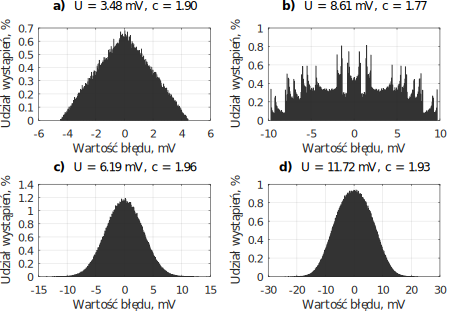
\includegraphics{obrazki/hist_part_a}
\DIFdelbeginFL %DIFDELCMD < \makecaption{fig:symul_parta_hist}{Histogramy realizacji sygnałów błędów \textbf{a)}~statycznego, \textbf{b)}~dynamicznego, \textbf{c)}~losowego, \textbf{d)}~wypadkowego, wielkości wyjściowej analizowanego w eksperymencie symulacyjnym przetwornika pomiarowego uzyskane metodą Monte-Carlo}
%DIFDELCMD < %%%
\DIFdelendFL \DIFaddbeginFL \makecaption{fig:symul_parta_hist}{Histogramy realizacji sygnałów błędów \textbf{a)}~statycznego, \textbf{b)}~dynamicznego, \textbf{c)}~losowego, \textbf{d)}~wypadkowego wielkości wyjściowej analizowanego w eksperymencie symulacyjnym przetwornika pomiarowego uzyskane metodą Monte-Carlo}
\DIFaddendFL \end{center}
\end{figure}

Wyznaczona na drodze eksperymentu wartość wielkości $U_{a,\Sigma}$ wyniosła~\qty{11.58}{mV}, przy czym wartość współczynnika rozszerzenia $c_{a,\Sigma}$ wyniosła~\num{1.90}. Wartość niepewności oszacowana na podstawie równania~\eqref{eq:sym_parta_uncert_value_a} jest zatem około~\qty{4.5}{\percent} większa od wartości uzyskanej na drodze eksperymentu. Należy zaznaczyć, że ta sama wartość wyznaczona za pomocą równania~\eqref{eq:sym_parta_uncert_sum} stosując współczynniki koherencji, których wartości zostały wyznaczone bez użycia zaproponowanej w pracy korekty opisanej równaniem~\eqref{eq:unc_cohercorra} wynosi~\qty{12.41}{mV}, a zatem jest ona o~\qty{7.3}{\percent} większa od wartości referencyjnej. W przypadku wartości oszacowanej na podstawie równania~\eqref{eq:sym_parta_uncert_value_b} rozbieżność jest nieco mniejsza i wynosi około~\qty{3.2}{\percent}, co dowodzi że w analizowanym przypadku spełnione zostały założenia związane z centralnym twierdzeniem granicznym, a przyjęte uproszczenia okazały się nie mieć znaczącego wpływu na wynik obliczeń. Uzyskana wartość wariancji sygnału błędu wypadkowego wielkości wyjściowej wyniosła w eksperymencie~\qty{37.1}{\micro V}, co pokrywa się z wartością wyznaczoną w równaniu~\eqref{eq:sym_parta_var_sum}. Wyznaczone w równaniach od~\eqref{eq:sym_parta_uncert_stat} do~\eqref{eq:sym_parta_factor_rand} parametry dla składowych sygnału błędu również w zadowalającym stopniu pokrywają się z uzyskanymi na drodze eksperymentu.

Zastosowana metoda szacowania wartości współczynników koherencji w celu wyznaczenia wypadkowej wartości niepewności rozszerzonej zapewnia wyniki zawyżone o kilka procent w stosunku do wartości uzyskiwanych symulacyjne. Jako, że omawiane rozbieżności są niewielkie oraz ich znak jest dodatni, uzyskiwane wyniki można uznać za prawidłowe. Wadą przedstawionej metody jest jednak konieczność znajomości wartości współczynników kształtu, co powoduje, że dla rozkładów o niestandardowym kształcie jej obszar zastosowań staje się ograniczony. Zaproponowana w pracy dodatkowa korekta wartości współczynników koherencji pozwala na uzyskanie bardziej zbliżonych, do uzyskiwanych symulacyjnie, wyników obliczeń.

Wobec przedstawionych rozważań i wyników przeprowadzonego eksperymentu stwierdzić można, że zaproponowany model błędów odpowiednio opisuje związki pomiędzy kolejnymi sygnałami błędów, zachodzące w analizowanym obiekcie. Jako, że kolejne fragmenty analizowanego toru pomiarowego przetwarzać będą zdefiniowane dotychczas sygnały błędów, przeprowadzony proces wyznaczania parametrów wypadkowych w przypadku grupy błędów dynamicznych oraz wyznaczanie parametrów wypadkowego błędu wielkości wyjściowej był nadmiarowy i został przeprowadzony jedynie w celu weryfikacji zaproponowanej metody obliczeń. W przypadku pozostałych grup sygnałów błędów, które cechowały się rozkładami o standardowych kształtach, wyznaczenie wypadkowych parametrów tych sygnałów pozwala na zmniejszenie liczby analizowanych sygnałów i upraszcza dalszą analizę.

\section{Analiza wzmacniacza pomiarowego}

Kolejną część toru pomiarowego stanowi wzmacniacz, którego zadaniem jest dopasowanie poziomu sygnału napięciowego $y_{a}(t)$, reprezentującego mierzoną wielkość fizyczną $s(t)$, do zakresu napięcia wejściowego $y_{b}(t)$ przetwornika analogowo-cyfrowego. Zakładane wzmocnienie układu wynosi $s_{b} = \qty{3.3}{V \per V}$, zatem w przypadku idealnym jego funkcję przetwarzania $\dot{f}_{b}(x)$ stanowi liniowa, addytywna funkcja opisana równaniem:
\begin{equation}
\dot{f}_{b} \emb{x} = s_{b} x = \num{3.3} x \label{eq:sym_partb_function},
\end{equation}
przy czym przyjęto, że nieliniowość przedstawionej charakterystyki jest pomijalnie mała i nie została rozważona w przedstawionym eksperymencie. Przyjąć można zatem założenie, że $\tilde{f}_{b}(x) \cong \dot{f}_{b}(x)$. Wobec powyższych, wielkość wyjściową analizowanego obiektu w przypadku idealnym oraz rzeczywistym opisać można jako:
\begin{gather}
\dot{y}_{b} \emb{t} = \dot{f}_{b} \emb{\dot{y}_{a} \emb{t}} = \num{3.3} \dot{y}_{a} \emb{t} \label{eq:sym_partb_out_ideal}, \\
\tilde{y}_{b} \emb{t} = \dot{y}_{b} \emb{t} + e_{b,\Sigma} \emb{t} \label{eq:sym_partb_out_real},
\end{gather}
gdzie sygnały wchodzące w skład wypadkowego sygnału błędu $e_{b,\Sigma}(t)$ opisano w dalszej części podrozdziału oraz wskazano ich parametry.

Analizowany układ wzmacniacza charakteryzuje się częstotliwością graniczną równą $f_{b,g} = \qty{650}{kHz}$, stąd zakłada się, że jego transmitancje opisać można w postaci:
\begin{equation}
\tilde{G}_{b} \emb{j\omega} = \frac{1}{1 + j \frac{\omega}{2 \pi f_{b,g}}} = \frac{1}{\frac{\omega^{2}}{4 \pi^{2} f_{b,g}^{2}} + 1} - j \frac{\omega}{2 \pi f_{b,g} \left( \frac{\omega^{2}}{4 \pi^{2} f_{b,g}^{2}} + 1 \right) } \label{eq:sym_partb_trans}.
\end{equation}
Wobec przedstawionego założenia, równania~\eqref{eq:mid_cont_amp} oraz~\eqref{eq:mid_cont_phi} można rozwinąć jako:
\begin{gather}
\tilde{K}_{b} \emb{\omega} = \sqrt{\left( \Re \left( \tilde{G}_{b} \emb{j\omega} \right) \right)^{2} + \left( \Im \left( \tilde{G}_{b} \emb{j\omega} \right) \right)^{2}} = \left( \frac{\omega^{2}}{4 \pi^{2} f_{b,g}^{2}} + 1 \right)^{-\frac{1}{2}} \label{eq:sym_partb_amp_real}, \\
\tilde{\varphi}_{b} \emb{\omega} = \arctan \left( \frac{\Im \left( \tilde{G}_{b} \emb{j\omega} \right)}{\Re \left( \tilde{G}_{b} \emb{j\omega} \right)} \right) = \arctan \left( -\frac{\omega}{2 \pi f_{b,g}} \right) \label{eq:sym_partb_phi_real},
\end{gather}
natomiast w przypadku idealnej transmitancji $\dot{G}_{b}(j\omega) = 1$ \DIFdelbegin \DIFdel{, }\DIFdelend parametry te wynoszą kolejno:
\begin{gather}
\dot{K}_{b} \emb{\omega} = \sqrt{\left( \Re \left( \dot{G}_{b} \emb{j\omega} \right) \right)^{2} + \left( \Im \left( \dot{G}_{b} \emb{j\omega} \right) \right)^{2}} = 1 \label{eq:sym_partb_amp_ideal}, \\
\dot{\varphi}_{b} \emb{\omega} = \arctan \left( \frac{\Im \left( \dot{G}_{b} \emb{j\omega} \right)}{\Re \left( \dot{G}_{b} \emb{j\omega} \right)} \right) = 0 \label{eq:sym_partb_phi_ideal}.
\end{gather}

Wobec przyjętych dotychczas założeń, opisanych w równaniach~\eqref{eq:sym_partb_out_ideal}, \eqref{eq:sym_partb_amp_ideal}, \eqref{eq:sym_partb_phi_ideal} oraz założenia określającego idealny przebieg przetwarzanej wielkości wejściowej $y_{a}(t)$, opisanego równaniem~\eqref{eq:sym_parta_out_ideal_sum}, idealny przebieg wielkości wyjściowej $y_{b}(t)$ w analizowanym przypadku określa równanie:
\begin{equation}
\dot{y}_{b} \emb{t} = \sum _{i=1} ^{3} E_{b,o} \emb{\omega_{b,i}} \sin \emb{\omega_{b,i} t + \varphi_{b,i}} \label{eq:sym_partb_out_ideal_sum},
\end{equation}
natomiast parametry kolejnych harmonicznych przedstawionego sygnału opisać można dla przypadku idealnego za pomocą równań:
\begin{gather}
E_{b,o} \emb{\omega} = \DIFdelbegin %DIFDELCMD < \dot{f}%%%
\DIFdelend \DIFaddbegin \DIFadd{s}\DIFaddend _{b} \DIFdelbegin %DIFDELCMD < \emb{\dot{K}_{b} \emb{\omega} E_{a,o} \emb{\omega}} %%%
\DIFdelend \DIFaddbegin \dot{K}\DIFadd{_{b} }\emb{\omega} \DIFadd{E_{a,o} }\emb{\omega} \DIFaddend = \num{3.3} E_{a,o} \emb{\omega} \label{eq:sym_partb_amp_out_ideal}, \\
\varphi_{b,o} \emb{\omega} = \varphi_{a,o} \emb{\omega} + \dot{\varphi}_{b} \emb{\omega} = \varphi_{a,o} \emb{\omega} \label{eq:sym_partb_phi_out_ideal},
\end{gather}
gdzie $E_{b,o}(\omega)$ jest amplitudą oraz $\varphi_{b,o}(\omega)$ fazą harmonicznej sygnału wyjściowego \DIFdelbegin \DIFdel{$y_{a}(t)$ }\DIFdelend \DIFaddbegin \DIFadd{$y_{b}(t)$ }\DIFaddend o wybranej pulsacji w przypadku idealnym, natomiast $\omega_{a,i} = \omega_{b,i}$ jest pulsacją $i$-tej harmonicznej analizowanego sygnału. Na podstawie danych zestawionych w tabeli~\ref{tab:sym_outa_params_ideal} oraz zależności od~\eqref{eq:sym_partb_out_ideal_sum} do~\eqref{eq:sym_partb_phi_out_ideal} wyznaczono parametry sygnału $y_{b}(t)$ dla przypadku idealnego i zestawiono je w tabeli~\ref{tab:sym_outb_params_ideal}.

\DIFdelbegin %DIFDELCMD < \begin{table}[htb!]
%DIFDELCMD < \begin{center}
%DIFDELCMD < \makecaption{tab:sym_outb_params_ideal}{Parametry kolejnych harmonicznych sygnału $y_{b}(t)$ przyjęte w przeprowadzanym eksperymencie symulacyjnym dla sytuacji idealnej}
%DIFDELCMD < \begin{tabular}[c]{| c | c | c | c |} \hline
%DIFDELCMD < \textbf{Lp. $i$} & \textbf{Pulsacja $\omega_{a,i}$, rad/s} & \textbf{Amplituda $E_{a,o}(\omega_{a,i})$, V} & \textbf{Faza $\varphi_{a,o}(\omega_{a,i})$, rad} \\ \hline
%DIFDELCMD < 1 & $1000  \cdot 2\pi$ &  \num{0.6} & $0$           \\ \hline
%DIFDELCMD < 2 & $5000  \cdot 2\pi$ &  \num{0.3} & $\pi/8 + \pi$ \\ \hline
%DIFDELCMD < 3 & $15000 \cdot 2\pi$ &  \num{0.1} & $\pi/6$       \\ \hline
%DIFDELCMD < \end{tabular}
%DIFDELCMD < \end{center}
%DIFDELCMD < \end{table}
%DIFDELCMD < %%%
\DIFdelend \DIFaddbegin \begin{table}[htb!]
\begin{center}
\makecaption{tab:sym_outb_params_ideal}{Parametry kolejnych harmonicznych sygnału $y_{b}(t)$ przyjęte w przeprowadzanym eksperymencie symulacyjnym dla sytuacji idealnej}
\begin{tabular}[c]{| c | c | c | c |} \hline
\textbf{$i$} & \textbf{Pulsacja $\omega_{b,i}$, rad/s} & \textbf{Amplituda $E_{b,o}(\omega_{b,i})$, V} & \textbf{Faza $\varphi_{b,o}(\omega_{b,i})$, rad} \\ \hline
1 & $1000  \cdot 2\pi$ &  \num{1.98} & $0$           \\ \hline
2 & $5000  \cdot 2\pi$ &  \num{0.99} & $\pi/8 + \pi$ \\ \hline
3 & $15000 \cdot 2\pi$ &  \num{0.33} & $\pi/6$       \\ \hline
\end{tabular}
\end{center}
\end{table}
\DIFaddend 

Pierwszą omawianą grupę sygnałów błędów stanowią błędy własne, wprowadzane przez analizowany obiekt. Przyjmuje się, że temperatura otoczenia $\vartheta(t)$ wpływa na dryft zera analizowanego wzmacniacza zgodnie z zależnością opisaną równaniem:
\begin{equation}
f_{b,z} \left( \vartheta \emb{t} \right) = \frac{7}{2} \left( \vartheta \emb{t} - \qty{20}{\degreeCelsius} \right)~\unit{\frac{mV}{K}} \label{eq:sym_partb_temp_err},
\end{equation}
oraz że w czasie wykonywania pojedynczej serii pomiarowej zmiany tej temperatury będą zbliżone do zera. Błąd statyczny własny, wynikający z dryftu zera spowodowanego zmianą temperatury otoczenia, zgodnie z równaniem~\eqref{eq:out_cont_err_env_self} opisać można jako:
\begin{equation}
e_{b,sw} \emb{t} = f_{b,z} \left( \vartheta \emb{t} \right) \label{eq:sym_partb_err_sw}.
\end{equation}
Sygnał błędu dynamicznego własnego, zdefiniowany w równaniach~\eqref{eq:mid_cont_err_dyn_prop} oraz~\eqref{eq:out_cont_err_dyn_prop}, opisać można na podstawie założeń danych równaniem~\eqref{eq:sym_parta_out_ideal_sum} w postaci:
\begin{equation}
e_{b,dw} \emb{t} = \sum \DIFdelbegin \DIFdel{_{i = j} }\DIFdelend \DIFaddbegin \DIFadd{_{i = 1} }\DIFaddend ^{3} e_{b,dw} \DIFdelbegin %DIFDELCMD < \emb{t,\omega_{a,j}} %%%
\DIFdelend \DIFaddbegin \emb{t,\omega_{a,i}} \DIFaddend = \sum \DIFdelbegin \DIFdel{_{i = j} }\DIFdelend \DIFaddbegin \DIFadd{_{i = 1} }\DIFaddend ^{3} E_{b,ew} \DIFdelbegin %DIFDELCMD < \emb{\omega_{b,j}} %%%
\DIFdelend \DIFaddbegin \emb{\omega_{b,i}} \DIFaddend \sin \DIFdelbegin %DIFDELCMD < \emb{\omega t + \varphi_{b,ew} \emb{\omega_{b,j}}} %%%
\DIFdelend \DIFaddbegin \emb{\omega t + \varphi_{b,ew} \emb{\omega_{b,i}}} \DIFaddend \label{eq:sym_partb_dyn_self_sum},
\end{equation}
natomiast kolejne harmoniczne przedstawionego sygnału mogą być opisane następująco:
\begin{equation}
\begin{split}
e_{b,dw} \emb{t,\omega} =~
& \tilde{f}_{b} \left( \tilde{K}_{b} \emb{\omega} E_{a,o} \emb{\omega} \sin \left( \omega t + \varphi_{a,o} \emb{\omega} + \tilde{\varphi}_{b} \emb{\omega} \right) \right)- \\
& \tilde{f}_{b} \left( \dot{K}_{b} \emb{\omega} E_{a,o} \emb{\omega} \sin \left( \omega t + \varphi_{a,o} \emb{\omega} + \dot{\varphi}_{b} \emb{\omega} \right) \right)
\end{split}
\label{eq:sym_partb_dyn_self_err}.
\end{equation}
\DIFdelbegin \DIFdel{Parametry składowych przetwarzanego }\DIFdelend \DIFaddbegin \DIFadd{Wypadkowe wartości parametrów amplitudy oraz fazy dla kolejnych harmonicznych }\DIFaddend sygnału \DIFdelbegin \DIFdel{$y_{a}(t)$ w funkcji pulsacji dla przypadku idealnego zdefiniowano w równaniach~\eqref{eq:sym_parta_amp_out_ideal} oraz ~\eqref{eq:sym_parta_phi_out_ideal}, natomiast }\DIFdelend \DIFaddbegin \DIFadd{błędu dynamicznego własnego $e_{b,dw}(t)$ zestawiono }\DIFaddend w tabeli~\DIFdelbegin \DIFdel{\ref{tab:sym_outb_params_ideal} zestawiono wyznaczone }\DIFdelend \DIFaddbegin \DIFadd{\ref{tab:sym_partb_params_dyn_self}, przy czym ich }\DIFaddend wartości \DIFdelbegin \DIFdel{tych parametrów dla przyjętych odnośnie przetwarzanego sygnału $s(t)$ założeń, danych równaniem~\eqref{eq:sym_in_ideal} i podsumowanych w tabeli~\ref{tab:sym_in_params_ideal}}\DIFdelend \DIFaddbegin \DIFadd{wyznaczono analogicznie, jak w przykładzie opisanym dla poprzedniej części toru pomiarowego w równaniach od~\eqref{eq:sym_parta_dyn_self_example_harm} do~\eqref{eq:sym_parta_dyn_self_example_phi}}\DIFaddend .

Drugą grupę sygnałów błędów stanowią błędy propagowane, przenoszone z wejścia na wyjście obiektu. Sygnał błędu statycznego $e_{a,sw}(t)$ jest przenoszony na wyjście obiektu zgodnie równaniami~\eqref{eq:mid_cont_err_stat_prop} oraz~\eqref{eq:out_cont_err_stat_prop}, zatem:
\begin{equation}
e_{b,sp} \emb{t} = \tilde{f}_{b} \left( \tilde{K}_{b} \emb{0} e_{a,sw} \emb{t} \right) = \num{3.3} e_{a,sw} \emb{t} \label{eq:sym_partb_stat_prop_err}\DIFdelbegin \DIFdel{,
}\DIFdelend \DIFaddbegin \DIFadd{.
}\DIFaddend \end{equation}
Sygnały błędów losowych $e_{a,rw}(t)$ oraz $e_{a,rp}(t)$ wielkości wejściowej są propagowane zgodnie z zależnością~\eqref{eq:out_cont_err_rand_prop}, przy czym ze względu na niedeterministyczny opis tych sygnałów nie ma możliwości zdefiniowania postaci tych sygnałów w funkcji czasu. Stosując zaproponowany model błędów należy jedynie zdefiniować parametry tych sygnałów na wyjściu obiektu, zatem przyjmuje się, że sygnał błędu $e_{b,rp,1}(t)$ na wyjściu obiektu związany jest z sygnałem $e_{a,rw}(t)$ na jego wejściu, oraz że sygnał $e_{b,rp,2}(t)$ na wyjściu obiektu jest powiązany z sygnałem $e_{a,rp}(t)$. Na podstawie wprowadzonych założeń wypadkowy sygnał propagowanego błędu losowego wyrazić można w postaci:
\begin{equation}
e_{b,rp} \emb{t} = e_{b,rp,1} \emb{t} + e_{b,rp,2} \emb{t} \label{eq:sym_partb_rand_prop_err}\DIFdelbegin \DIFdel{,
}\DIFdelend \DIFaddbegin \DIFadd{.
}\DIFaddend \end{equation}
Przetwarzany przez obiekt sygnał błędu dynamicznego $e_{a,dw}(t)$ propagowany jest na wyjście zgodnie z równaniami~\eqref{eq:mid_cont_err_dyn_prop} oraz~\eqref{eq:out_cont_err_dyn_prop}, zatem wybraną harmoniczną sygnału propagowanego błędu dynamicznego $e_{b,dp}(t)$ na wyjściu tego obiektu opisuje równanie:
\begin{equation}
\DIFdelbegin %DIFDELCMD < \begin{split}
%DIFDELCMD < e_{b,dp} \emb{t,\omega} =~
%DIFDELCMD < & \dot{f}_{b} \left( \tilde{K}_{b} \emb{\omega} E_{a,e} \emb{\omega} \sin \left( \omega t + \varphi_{a,e} \emb{\omega} + \tilde{\varphi}_{b} \emb{\omega} \right) \right) = \\
%DIFDELCMD < & \num{3.3} \tilde{K}_{b} \emb{\omega} E_{a,e} \emb{\omega} \sin \left( \omega t + \varphi_{a,e} \emb{\omega} + \tilde{\varphi}_{b} \emb{\omega} \right)
%DIFDELCMD < \end{split}%%%
\DIFdelend \DIFaddbegin \begin{split}
e_{b,dp} \emb{t,\omega} =~
& \tilde{f}_{b} \left( \tilde{K}_{b} \emb{\omega} E_{a,e} \emb{\omega} \sin \left( \omega t + \varphi_{a,e} \emb{\omega} + \tilde{\varphi}_{b} \emb{\omega} \right) \right) = \\
& \num{3.3} \tilde{K}_{b} \emb{\omega} E_{a,e} \emb{\omega} \sin \left( \omega t + \varphi_{a,e} \emb{\omega} + \tilde{\varphi}_{b} \emb{\omega} \right)
\end{split}\DIFaddend 
\label{eq:sym_partb_dyn_prop_err},
\end{equation}
\DIFdelbegin \DIFdel{natomiast }\DIFdelend \DIFaddbegin \DIFadd{gdzie }\DIFaddend wypadkowe parametry kolejnych harmonicznych \DIFdelbegin \DIFdel{przetwarzanego }\DIFdelend \DIFaddbegin \DIFadd{$e_{a,dp}(t,\omega)$ omawianego }\DIFaddend sygnału \DIFdelbegin \DIFdel{błędu dynamicznego $e_{a,dw}(t)$ }\DIFdelend zestawiono w tabeli~\ref{tab:sym_parta_params_dyn_summary}. Wypadkowy sygnał błędu dynamicznego propagowanego \DIFaddbegin \DIFadd{$e_{b,dp}(t)$ na wyjściu analizowanego obiektu }\DIFaddend zdefiniować można zatem jako:
\begin{equation}
e_{b,dp} \emb{t} = \sum \DIFdelbegin \DIFdel{_{j = 1} }\DIFdelend \DIFaddbegin \DIFadd{_{i = 1} }\DIFaddend ^{3} e_{b,dp} \DIFdelbegin %DIFDELCMD < \emb{t,\omega_{a,j}} %%%
\DIFdelend \DIFaddbegin \emb{t,\omega_{a,i}} \DIFaddend = \sum \DIFdelbegin \DIFdel{_{i = j} }\DIFdelend \DIFaddbegin \DIFadd{_{i = 1} }\DIFaddend ^{3} E_{b,ep} \DIFdelbegin %DIFDELCMD < \emb{\omega_{b,j}} %%%
\DIFdelend \DIFaddbegin \emb{\omega_{b,i}} \DIFaddend \sin \DIFdelbegin %DIFDELCMD < \emb{\omega t + \varphi_{b,ep} \emb{\omega_{b,j}}} %%%
\DIFdelend \DIFaddbegin \emb{\omega t + \varphi_{b,ep} \emb{\omega_{b,i}}} \DIFaddend \label{eq:sym_partb_dyn_prop_sum},
\end{equation}
przy czym omówiony przypadek dotyczy założeń przyjętych w równaniu~\eqref{eq:sym_parta_dyn_self_sum}, które wynikają z założonej w równaniu~\eqref{eq:sym_in_ideal} postaci sygnału $s(t)$.

Parametry wypadkowe kolejnych harmonicznych sygnałów błędów dynamicznych własnych $e_{b,dw}(t)$ oraz propagowanych $e_{b,dp}(t)$ mogą być wyznaczone w sposób analogiczny, jak pokazano na przykładnie opisanym w równaniach od~\eqref{eq:sym_parta_dyn_self_example_sum} do~\eqref{eq:sym_parta_dyn_self_example_phi}. Wyznaczenie omawianych parametrów pozwoli na określenie wartości wariancji wymienionych sygnałów oraz wyznaczenie związanej z nimi wartości niepewności rozszerzonej. Wyznaczone zgodnie z metodą zaproponowaną w równaniach od~\eqref{eq:dyn_vect} do~\eqref{eq:dyn_vect_phi} wypadkowe amplitudy oraz fazy dla wskazanych sygnałów błędów dynamicznych przedstawiono w tabelach~\ref{tab:sym_partb_params_dyn_self} oraz~\ref{tab:sym_partb_params_dyn_prop}. Należy zauważyć, \DIFaddbegin \DIFadd{że }\DIFaddend wyznaczenie wypadkowych parametrów kolejnych harmonicznych analizowanych sygnałów nie jest konieczne z punktu widzenia stosowania zaproponowanego modelu błędów. Zabieg ten pozwala natomiast uprościć analizę poprzez redukcję liczby analizowanych sygnałów.

\DIFdelbegin %DIFDELCMD < \begin{table}[htb!]
%DIFDELCMD < \begin{center}
%DIFDELCMD < \makecaption{tab:sym_partb_params_dyn_self}{Parametry wypadkowe kolejnych harmonicznych sygnału błędu dynamicznego własnego analizowanego w eksperymencie symulacyjnym wzmacniacza pomiarowego}
%DIFDELCMD < \begin{tabular}[c]{| c | c | S[table-format = 2.2] | S[table-format = +1.2] |} \hline
%DIFDELCMD < \textbf{Lp. $j$} & \textbf{Pulsacja $\omega_{b,j}$, rad/s} & \textbf{Amplituda $E_{b,e}(\omega_{b,j})$, mV} & \textbf{Faza $\varphi_{b,e}(\omega_{b,j})$, rad} \\ \hline
%DIFDELCMD < 1 & $1000  \cdot 2\pi$  &   3.05  & -1.57  \\ \hline
%DIFDELCMD < 2 & $5000  \cdot 2\pi$  &   7.62  &  1.96  \\ \hline
%DIFDELCMD < 3 & $15000 \cdot 2\pi$  &   7.61  & -1.06  \\ \hline
%DIFDELCMD < \end{tabular}
%DIFDELCMD < \end{center}
%DIFDELCMD < \end{table}
%DIFDELCMD < %%%
\DIFdelend \DIFaddbegin \begin{table}[htb!]
\begin{center}
\makecaption{tab:sym_partb_params_dyn_self}{Parametry wypadkowe kolejnych harmonicznych sygnału błędu dynamicznego własnego analizowanego w eksperymencie symulacyjnym wzmacniacza pomiarowego}
\begin{tabular}[c]{| c | c | S[table-format = 2.2] | S[table-format = +1.2] |} \hline
\textbf{$i$} & \textbf{Pulsacja $\omega_{b,i}$, rad/s} & \textbf{Amplituda $E_{b,ew}(\omega_{b,i})$, mV} & \textbf{Faza $\varphi_{b,ew}(\omega_{b,i})$, rad} \\ \hline
1 & $1000  \cdot 2\pi$  &   3.05  & -1.57  \\ \hline
2 & $5000  \cdot 2\pi$  &   7.62  &  1.96  \\ \hline
3 & $15000 \cdot 2\pi$  &   7.61  & -1.06  \\ \hline
\end{tabular}
\end{center}
\end{table}
\DIFaddend 

\DIFdelbegin %DIFDELCMD < \begin{table}[htb!]
%DIFDELCMD < \begin{center}
%DIFDELCMD < \makecaption{tab:sym_partb_params_dyn_prop}{Parametry wypadkowe kolejnych harmonicznych sygnału błędu dynamicznego propagowanego analizowanego w eksperymencie symulacyjnym wzmacniacza pomiarowego}
%DIFDELCMD < \begin{tabular}[c]{| c | c | S[table-format = 2.2] | S[table-format = +1.2] |} \hline
%DIFDELCMD < \textbf{Lp. $j$} & \textbf{Pulsacja $\omega_{b,j}$, rad/s} & \textbf{Amplituda $E_{b,e}(\omega_{b,j})$, mV} & \textbf{Faza $\varphi_{b,e}(\omega_{b,j})$, rad} \\ \hline
%DIFDELCMD < 1 & $1000  \cdot 2\pi$  &   6.19  & -1.57  \\ \hline
%DIFDELCMD < 2 & $5000  \cdot 2\pi$  &  15.47  &  1.95  \\ \hline
%DIFDELCMD < 3 & $15000 \cdot 2\pi$  &  15.46  & -1.09  \\ \hline
%DIFDELCMD < \end{tabular}
%DIFDELCMD < \end{center}
%DIFDELCMD < \end{table}
%DIFDELCMD < %%%
\DIFdelend \DIFaddbegin \begin{table}[htb!]
\begin{center}
\makecaption{tab:sym_partb_params_dyn_prop}{Parametry wypadkowe kolejnych harmonicznych sygnału błędu dynamicznego propagowanego analizowanego w eksperymencie symulacyjnym wzmacniacza pomiarowego}
\begin{tabular}[c]{| c | c | S[table-format = 2.2] | S[table-format = +1.2] |} \hline
\textbf{$i$} & \textbf{Pulsacja $\omega_{b,i}$, rad/s} & \textbf{Amplituda $E_{b,ep}(\omega_{b,i})$, mV} & \textbf{Faza $\varphi_{b,ep}(\omega_{b,i})$, rad} \\ \hline
1 & $1000  \cdot 2\pi$  &   6.19  & -1.57  \\ \hline
2 & $5000  \cdot 2\pi$  &  15.47  &  1.95  \\ \hline
3 & $15000 \cdot 2\pi$  &  15.46  & -1.09  \\ \hline
\end{tabular}
\end{center}
\end{table}
\DIFaddend 

Cel następnego etapu rozważań stanowi określenie parametrów wariancji oraz niepewności rozszerzonych dla opisanych dotychczas sygnałów błędów. Ze względu na liniowy charakter analizowanego obiektu, wynikający z przyjętych założeń, opisanych w równaniach~\eqref{eq:sym_partb_out_ideal} oraz~\eqref{eq:sym_partb_trans}, na wyjściu obiektu zachowane zostaną oryginalne kształty rozkładów wszystkich propagowanych sygnałów błędów~\cite{grimmett_probability}. Wobec powyższych, znając wariancję tych sygnałów na wyjściu obiektu, wyznaczenie związanej z nimi wartości niepewności rozszerzonej odbywać się może zgodnie z zależnością~\eqref{eq:unc_sum}. Wpływ transmitancji obiektu na wartość wariancji propagowanych sygnałów błędów opisany został wcześniej równaniem~\eqref{eq:mid_cont_var_omega}, natomiast wpływ funkcji przetwarzania na tą wielkość, w przypadku liniowej funkcji przetwarzania, określa zależność~\eqref{eq:out_cont_var_sense}. Można zatem zapisać, w przypadku sygnału propagowanego błędu statycznego:
\begin{gather}
\sigma_{b,sp}^{2} = s_{b}^{2} \tilde{K}_{b}^{2} \emb{0} \sigma_{a,sw}^{2} = \num{3.3}^{2} \cdot \num{1.0}^{2} \cdot \DIFdelbegin %DIFDELCMD < \num{3.38} %%%
\DIFdelend \DIFaddbegin \num{3.38e-6} \DIFaddend = \qty{36.75}{\micro V} \label{eq:sym_partb_var_stat_prop}, \\
U_{b,sp} = c_{b,sp} \sigma_{b,sp} = \qty{11.52}{mV} \label{eq:sym_partb_unc_stat_prop},
\end{gather}
\DIFdelbegin \DIFdel{gdzie }\DIFdelend \DIFaddbegin \DIFadd{przy czym }\DIFaddend $c_{b,sp} = c_{a,sw} = c_{t} = \num{1.90}$. W przypadku \DIFdelbegin \DIFdel{kolejnych harmonicznych }\DIFdelend \DIFaddbegin \DIFadd{wypadkowego }\DIFaddend sygnału błędu dynamicznego \DIFdelbegin \DIFdel{, ich wariancję }\DIFdelend \DIFaddbegin \DIFadd{$e_{b,d}(t)$ wariancje kolejnych składowych tego sygnału }\DIFaddend opisać można zgodnie z zależnością~\eqref{eq:dyn_var}\DIFdelbegin \DIFdel{na podstawie wypadkowych parametrów tych harmonicznych, zestawionych }\DIFdelend \DIFaddbegin \DIFadd{, przy czym parametry jego harmonicznych zestawiono }\DIFaddend w tabelach~\ref{tab:sym_partb_params_dyn_self} oraz~\ref{tab:sym_partb_params_dyn_prop}. \DIFdelbegin \DIFdel{Wariancję }\DIFdelend \DIFaddbegin \DIFadd{Wariancje }\DIFaddend sygnałów błędów losowych $e_{b,rp,1}(t)$ oraz $e_{b,rp,2}(t)$ można natomiast opisać w funkcji pulsacji, jako:
\begin{gather}
\sigma_{b,rp,1}^{2} \emb{\omega} = s_{b}^{2} \tilde{K}_{b} \emb{\omega} \sigma_{a,rw}^{2} \emb{\omega} \cong \qty{36.26}{\micro V} \label{eq:sym_partb_var_rand_prop_1}, \\
\sigma_{b,rp,2}^{2} \emb{\omega} = s_{b}^{2} \tilde{K}_{b} \emb{\omega} \sigma_{a,rp}^{2} \emb{\omega} = s_{a}^{2} s_{b}^{2} \tilde{K}_{a}^{2} \emb{\omega} \tilde{K}_{b} \emb{\omega} \sigma_{s,r}^{2} \emb{\omega} \cong \qty{72.64}{\micro V} \label{eq:sym_partb_var_rand_prop_2},
\end{gather}
przy czym postać przedstawionych zależności wynika z faktu, że w zakresie częstotliwości \DIFdelbegin \DIFdel{$\hat{f} \in~<0;\frac{1}{2} f_{p}>$ }\DIFdelend \DIFaddbegin \DIFadd{$\hat{f} \in \interval{0}{\frac{1}{2} f_{p}}$ }\DIFaddend transmitancja obiektu nie wpływa na widmo przetwarzanych sygnałów błędów losowych. Można zatem, zgodnie z zależnością~\eqref{eq:out_cont_err_rand_prop}, przyjąć założenia gdzie \DIFdelbegin \DIFdel{$e_{b,rp,1}(t) = \tilde{f}_{b}(e_{a,rw}(t))$ oraz $e_{b,rp,2}(t) = \tilde{f}_{b}(e_{a,rp}(t))$}\DIFdelend \DIFaddbegin \DIFadd{$e_{b,rp,1}(t) \cong \tilde{f}_{b}(e_{a,rw}(t))$ oraz $e_{b,rp,2}(t) \cong \tilde{f}_{b}(e_{a,rp}(t))$}\DIFaddend . Wartości niepewności rozszerzonych związanych z analizowanymi sygnałami opisują zatem równania:
\begin{gather}
U_{b,rp,1} = c_{b,rp,1} \sigma_{b,rp,1} = \qty{9.93}{mV} \label{eq:sym_partb_uncert_rand_prop_1}, \\
U_{b,rp,2} = c_{b,rp,2} \sigma_{b,rp,2} = \qty{16.70}{mV} \label{eq:sym_partb_uncert_rand_prop_2},
\end{gather}
gdzie $c_{b,rp,1} = c_{a,rw} = c_{u} = \num{1.65}$ oraz $c_{b,rp,2} = c_{a,rp} = c_{n} = \num{1.96}$. Należy zauważyć, że w przypadku istnienia wpływu transmitancji obiektu na widmową gęstość mocy analizowanych sygnałów, w celu wyznaczenia wartości niepewności rozszerzonej związanej z tymi sygnałami należałoby określić średnią wartość wariancji tych sygnałów dla analizowanego zakresu częstotliwości, określoną równaniem~\eqref{eq:mid_cont_var_rand}. Tabela~\ref{tab:sym_partb_params_unc_list} przedstawia budżet niepewności wielkości wyjściowej analizowanego wzmacniacza pomiarowego z uwzględnieniem podziału na sygnały błędów własnych i propagowanych, sporządzony na podstawie przedstawionych rozważań.

\DIFdelbegin %DIFDELCMD < \begin{table}[htb!]
%DIFDELCMD < \begin{center}
%DIFDELCMD < \makecaption{tab:sym_partb_params_unc_list}{Budżet niepewności wielkości wyjściowej analizowanego w eksperymencie symulacyjnym wzmacniacza pomiarowego, gdzie (a)~oznacza przetwornik pomiarowy oraz (b)~oznacza wzmacniacz pomiarowy}
%DIFDELCMD < \begin{tabular}[c]{| c | c | S[table-format = 2.2] | S[table-format = 3.2] | c | c |} \hline
%DIFDELCMD < \textbf{Lp.} & \textbf{Symbol} & \textbf{$U$, mV} & \textbf{$\sigma^{2}$, \micro V} & \textbf{Rozkład} & \textbf{Źródło błędu} \\ \hline
%DIFDELCMD < 1  & ${b,sp}$       & 11.52 &  36.75  & trójkątny                    & dryft temperatury (a)                       \\ \hline
%DIFDELCMD < 2  & ${b,sw}$       & 8.15  &  18.38  & trójkątny                    & dryft temperatury (b)                       \\ \hline
%DIFDELCMD < 3  & ${b,rp,1}$     & 9.93  &  36.26  & jednostajny                  & nieliniowość obiektu (a)                   \\ \hline
%DIFDELCMD < 4  & ${b,rp,2}$     & 16.70 &  72.64  & normalny                     & szum wielkości wejściowej                  \\ \hline
%DIFDELCMD < 5  & ${b,dp,1}$     & 6.21  &  19.14  & \multirow{6}{*}{dwumodalny}  & \multirow{3}{*}{transmitancja (a)}         \\ \cline{1-4}
%DIFDELCMD < 6  & ${b,dp,2}$     & 15.53 &  119.62 &                              &                                            \\ \cline{1-4}
%DIFDELCMD < 7  & ${b,dp,3}$     & 15.52 &  119.44 &                              &                                            \\ \cline{1-4} \cline{6-6}
%DIFDELCMD < 8  & ${b,dw,1}$     & 3.06  &  4.64   &                              & \multirow{3}{*}{transmitancja (b)}         \\ \cline{1-4}
%DIFDELCMD < 9  & ${b,dw,2}$     & 7.65  &  29.00  &                              &                                            \\ \cline{1-4}
%DIFDELCMD < 10 & ${b,dw,3}$     & 7.65  &  28.99  &                              &                                            \\ \hline
%DIFDELCMD < \end{tabular}
%DIFDELCMD < \end{center}
%DIFDELCMD < \end{table}
%DIFDELCMD < %%%
\DIFdelend \DIFaddbegin \begin{table}[htb!]
\begin{center}
\makecaption{tab:sym_partb_params_unc_list}{Budżet niepewności wielkości wyjściowej analizowanego w eksperymencie symulacyjnym wzmacniacza pomiarowego, gdzie ($a$)~oznacza przetwornik pomiarowy oraz ($b$)~oznacza wzmacniacz pomiarowy}
\begin{tabular}[c]{| c | c | S[table-format = 2.2] | S[table-format = 3.2] | c | c |} \hline
\textbf{Lp.} & \textbf{Symbol} & \textbf{$U$, mV} & \textbf{$\sigma^{2}$, \micro V} & \textbf{Rozkład} & \textbf{Źródło błędu} \\ \hline
1  & ${b,sp}$       & 11.52 &  36.75  & trójkątny                    & dryft temperatury ($a$)                    \\ \hline
2  & ${b,sw}$       & 8.15  &  18.38  & trójkątny                    & dryft temperatury ($b$)                    \\ \hline
3  & ${b,rp,1}$     & 9.93  &  36.26  & jednostajny                  & nieliniowość obiektu ($a$)                 \\ \hline
4  & ${b,rp,2}$     & 16.70 &  72.64  & normalny                     & szum wielkości wejściowej                  \\ \hline
5  & ${b,dp,1}$     & 6.21  &  19.14  & \multirow{6}{*}{dwumodalny}  & \multirow{3}{*}{transmitancja ($a$)}       \\ \cline{1-4}
6  & ${b,dp,2}$     & 15.53 &  119.62 &                              &                                            \\ \cline{1-4}
7  & ${b,dp,3}$     & 15.52 &  119.44 &                              &                                            \\ \cline{1-4} \cline{6-6}
8  & ${b,dw,1}$     & 3.06  &  4.64   &                              & \multirow{3}{*}{transmitancja ($b$)}       \\ \cline{1-4}
9  & ${b,dw,2}$     & 7.65  &  29.00  &                              &                                            \\ \cline{1-4}
10 & ${b,dw,3}$     & 7.65  &  28.99  &                              &                                            \\ \hline
\end{tabular}
\end{center}
\end{table}
\DIFaddend 

Dla źródeł błędów wymienionych w budżecie niepewności, zestawionym w tabeli~\ref{tab:sym_partb_params_unc_list}, konieczne jest określenie wzajemnych korelacji pomiędzy sygnałami błędów. Należy zauważyć, że składowe związane z dryftem temperaturowym przetwornika pomiarowego oraz dryftem temperaturowym wzmacniacza zależą od tej samej wielkości fizycznej -- temperatury otoczenia. Jako, że wymienione sygnały błędów nie zależą od żadnej innej wielkości, a dodatkowo równania~\eqref{eq:sym_parta_stat_err} oraz~\eqref{eq:sym_partb_temp_err} cechują się dodatnią czułością względem tej wielkości, można założyć pełną dodatnią korelacje analizowanych sygnałów błędów, zatem $r_{b,sw,b,sp} = r_{b,sp,b,sw} = 1$. W przypadku kolejnych harmonicznych sygnałów błędów dynamicznych wartość współczynnika korelacji tych składowych może być obliczona zgodnie z równaniem~\eqref{eq:dyn_corr}. Można zauważyć, że wartość tego współczynnika dla par składowych o różnej pulsacji każdorazowo wyniesie zero. W przypadku par harmonicznych sygnałów błędów dynamicznych o identycznej pulsacji, na podstawie danych zawartych w tabelach~\ref{tab:sym_partb_params_dyn_self} oraz~\ref{tab:sym_partb_params_dyn_prop}, zauważyć można, że współczynnik korelacji zbliżony będzie od jedności, ze względu na zbliżoną do zera różnicę w fazach tych sygnałów. W przypadku pozostałych par sygnałów wartości współczynników korelacji będą zerowe.

Biorąc pod uwagę przedstawione informacje na temat istniejących korelacji pomiędzy analizowanymi sygnałami błędów należy zauważyć, że zastosowanie opisanej równaniem~\eqref{eq:unc_matrix} metody wyznaczania wypadkowej wartości niepewności rozszerzonej nie będzie możliwe dla wartości współczynników koherencji wyznaczanych zgodnie z równaniem~\eqref{eq:unc_coher}. Ograniczenie to wynika z faktu, że opisane w równaniach~\eqref{eq:unc_cohercorra} oraz~\eqref{eq:unc_cohercorrb} korekty\DIFaddbegin \DIFadd{, a także wartości współczynników kształtu, wyznaczane zgodnie z równaniem~\eqref{eq:unc_shapertwo}, }\DIFaddend nie są odpowiednie dla sytuacji, gdzie pomiędzy analizowanymi sygnałami występuje korelacja. Proponuje się zatem, w celu umożliwienia zastosowania przedstawionej metody analizy, wyznaczenie wypadkowych parametrów wariancji i niepewności rozszerzonych dla skorelowanych grup sygnałów. Jako, że zaproponowana operacja prowadzi do redukcji liczby analizowanych sygnałów błędów poprzez wprowadzenie wypadkowych sygnałów dla analizowanych grup, proponuje się równolegle określić budżet niepewności dla rozważanego fragmentu toru pomiarowego, który zorientowany będzie pod kątem charakteru realizacji wymienionych w nim sygnałów.

Na podstawie zależności od~\eqref{eq:sym_partb_err_sw} do~\eqref{eq:sym_partb_dyn_prop_sum}, zgodnie z równaniem~\eqref{eq:out_cont_err_sum_all}, opisać można wprowadzony w równaniu~\eqref{eq:sym_partb_out_real} wypadkowy sygnał błędu $e_{b,\Sigma}(t)$ wielkości wyjściowej analizowanego wzmacniacza pomiarowego następującym równaniem:
\begin{equation}
e_{b,\Sigma} \emb{t} = e_{b,s} \emb{t} + e_{b,d} \emb{t} + e\DIFdelbegin \DIFdel{_{b,s} }\DIFdelend \DIFaddbegin \DIFadd{_{b,r} }\DIFaddend \emb{t} \label{eq:sym_partb_error_sum},
\end{equation}
w którym kolejne składniki przedstawionego sygnału zdefiniowane są w postaci:
\begin{gather}
e_{b,s} \emb{t} = e_{b,sw} \emb{t} + e_{b,sp} \emb{t} \label{eq:sym_partb_error_stat}, \\
e_{b,d} \emb{t} = e_{b,dw} \emb{t} + e_{b,dp} \emb{t} \label{eq:sym_partb_error_dyn}, \\
e_{b,r} \emb{t} = e_{b,rp} \emb{t} \label{eq:sym_partb_error_rand},
\end{gather}
gdzie $e_{b,s}(t)$ jest wypadkowym sygnałem błędu statycznego, $e_{b,d}(t)$ dynamicznego oraz $e_{b,r}(t)$ losowego. Wypadkowy sygnał błędu dynamicznego opisać można w postaci:
\begin{equation}
e_{b,d} \emb{t} = \sum \DIFdelbegin \DIFdel{_{k=1} }\DIFdelend \DIFaddbegin \DIFadd{_{i=1} }\DIFaddend ^{3} E_{b,e} \DIFdelbegin %DIFDELCMD < \emb{\omega_{b,k}} %%%
\DIFdelend \DIFaddbegin \emb{\omega_{b,i}} \DIFaddend \sin \DIFdelbegin %DIFDELCMD < \emb{\omega t + \varphi_{b,e} \emb{\omega_{b,k}}} %%%
\DIFdelend \DIFaddbegin \emb{\omega t + \varphi_{b,e} \emb{\omega_{b,i}}} \DIFaddend \label{sym_partb_error_dyn_sum},
\end{equation}
przy czym $E_{b,e}(\omega)$ jest wypadkową amplitudą, natomiast $\varphi_{b,e}(\omega)$ wypadkową fazą harmonicznej tego sygnału o wskazanej pulsacji. Wyznaczenie wypadkowych wartości amplitudy oraz fazy dla kolejnych harmonicznych sygnału błędu dynamicznego $e_{b,d}(t)$ przebiega zgodnie z metodą zaproponowaną w równaniach od~\eqref{eq:dyn_vect} do~\eqref{eq:dyn_vect_phi}, przy czym kolejne składniki tych harmonicznych wymienione \DIFdelbegin \DIFdel{są }\DIFdelend \DIFaddbegin \DIFadd{zostały }\DIFaddend w równaniach~\eqref{eq:sym_partb_dyn_self_err} oraz~\eqref{eq:sym_partb_dyn_prop_err}. Przedstawiony proces odbywać się może również z wykorzystaniem parametrów opisanych w tabelach~\ref{tab:sym_partb_params_dyn_self} oraz~\ref{tab:sym_partb_params_dyn_prop}, przy czym niezależnie od stosowanej metody uzyskuje się identyczne wyniki obliczeń. Wartości omawianych parametrów\DIFaddbegin \DIFadd{, }\DIFaddend wyznaczone zgodnie z przedstawionymi zależnościami\DIFaddbegin \DIFadd{, }\DIFaddend zestawiono w tabeli~\ref{tab:sym_partb_params_dyn_summary}.

\DIFdelbegin %DIFDELCMD < \begin{table}[htb!]
%DIFDELCMD < \begin{center}
%DIFDELCMD < \makecaption{tab:sym_partb_params_dyn_summary}{Parametry wypadkowe kolejnych harmonicznych sygnału błędu dynamicznego analizowanego w eksperymencie symulacyjnym wzmacniacza pomiarowego}
%DIFDELCMD < \begin{tabular}[c]{| c | c | S[table-format = 2.2] | S[table-format = +1.2] |} \hline
%DIFDELCMD < \textbf{Lp. $k$} & \textbf{Pulsacja $\omega_{b,k}$, rad/s} & \textbf{Amplituda $E_{b,e}(\omega_{b,k})$, mV} & \textbf{Faza $\varphi_{b,e}(\omega_{b,k})$, rad} \\ \hline
%DIFDELCMD < 1 & $1000  \cdot 2\pi$  &   9.23  & -1.57  \\ \hline
%DIFDELCMD < 2 & $5000  \cdot 2\pi$  &  23.08  &  1.96  \\ \hline
%DIFDELCMD < 3 & $15000 \cdot 2\pi$  &  23.07  & -1.07  \\ \hline
%DIFDELCMD < \end{tabular}
%DIFDELCMD < \end{center}
%DIFDELCMD < \end{table}
%DIFDELCMD < %%%
\DIFdelend \DIFaddbegin \begin{table}[htb!]
\begin{center}
\makecaption{tab:sym_partb_params_dyn_summary}{Parametry wypadkowe kolejnych harmonicznych sygnału błędu dynamicznego analizowanego w eksperymencie symulacyjnym wzmacniacza pomiarowego}
\begin{tabular}[c]{| c | c | S[table-format = 2.2] | S[table-format = +1.2] |} \hline
\textbf{$i$} & \textbf{Pulsacja $\omega_{b,i}$, rad/s} & \textbf{Amplituda $E_{b,e}(\omega_{b,i})$, mV} & \textbf{Faza $\varphi_{b,e}(\omega_{b,i})$, rad} \\ \hline
1 & $1000  \cdot 2\pi$  &   9.23  & -1.57  \\ \hline
2 & $5000  \cdot 2\pi$  &  23.08  &  1.96  \\ \hline
3 & $15000 \cdot 2\pi$  &  23.07  & -1.07  \\ \hline
\end{tabular}
\end{center}
\end{table}
\DIFaddend 

Parametry wypadkowego \DIFaddbegin \DIFadd{sygnału }\DIFaddend błędu statycznego \DIFdelbegin \DIFdel{, danego }\DIFdelend \DIFaddbegin \DIFadd{$e_{b,s}(t)$, zdefiniowanego }\DIFaddend zależnością~\eqref{eq:sym_partb_error_stat}, opisują równania~\eqref{eq:var_matrix} oraz~\eqref{eq:unc_matrix}, przy czym\DIFdelbegin \DIFdel{w bieżącym przypadku przyjmują one postać:
}\DIFdelend \DIFaddbegin \DIFadd{:
}\DIFaddend \begin{gather}
\DIFdelbegin %DIFDELCMD < \begin{split}
%DIFDELCMD < \sigma_{b,s}^{2} = ~ &
%DIFDELCMD < \begin{bmatrix}
%DIFDELCMD < \sigma_{b,sw} \\ \sigma_{b,sp}
%DIFDELCMD < \end{bmatrix}^{T}
%DIFDELCMD < \begin{bmatrix}
%DIFDELCMD < 1 & r_{b,sw,sp} \\
%DIFDELCMD < r_{b,sp,rw} & 1
%DIFDELCMD < \end{bmatrix}
%DIFDELCMD < \begin{bmatrix}
%DIFDELCMD < \sigma_{b,sw} \\ \sigma_{b,sp}
%DIFDELCMD < \end{bmatrix} = \\ &
%DIFDELCMD < \begin{bmatrix}
%DIFDELCMD < \num{6.06e-3} \\ \num{4.29e-3}
%DIFDELCMD < \end{bmatrix}^{T}
%DIFDELCMD < \begin{bmatrix}
%DIFDELCMD < 1 & 1 \\
%DIFDELCMD < 1 & 1
%DIFDELCMD < \end{bmatrix}
%DIFDELCMD < \begin{bmatrix}
%DIFDELCMD < \num{6.06e-3} \\ \num{4.29e-3}
%DIFDELCMD < \end{bmatrix} = \qty{107.12}{\micro V}
%DIFDELCMD < \end{split}%%%
\DIFdelend \DIFaddbegin \begin{split}
\sigma_{b,s}^{2} = ~ &
\begin{bmatrix}
\sigma_{b,sw} \\ \sigma_{b,sp}
\end{bmatrix}^{T}
\begin{bmatrix}
1 & r_{b,sw,sp} \\
r_{b,sp,sw} & 1
\end{bmatrix}
\begin{bmatrix}
\sigma_{b,sw} \\ \sigma_{b,sp}
\end{bmatrix} = \\ &
\begin{bmatrix}
\num{6.06e-3} \\ \num{4.29e-3}
\end{bmatrix}^{T}
\begin{bmatrix}
1 & 1 \\
1 & 1
\end{bmatrix}
\begin{bmatrix}
\num{6.06e-3} \\ \num{4.29e-3}
\end{bmatrix} = \qty{107.12}{\micro V}
\end{split}\DIFaddend 
\label{eq:sym_partb_stat_var}\DIFdelbegin \DIFdel{. }\DIFdelend \DIFaddbegin \DIFadd{, }\DIFaddend \\
\DIFdelbegin %DIFDELCMD < \begin{split}
%DIFDELCMD < U_{b,s} = ~ & \sqrt{
%DIFDELCMD < \begin{bmatrix}
%DIFDELCMD < U_{b,sw} \\ U_{b,sp}
%DIFDELCMD < \end{bmatrix}^{T}
%DIFDELCMD < \begin{bmatrix}
%DIFDELCMD < 1 & h_{b,sw,sp} \\
%DIFDELCMD < h_{b,sp,rw} & 1
%DIFDELCMD < \end{bmatrix}
%DIFDELCMD < \begin{bmatrix}
%DIFDELCMD < U_{b,sw} \\ U_{b,sp}
%DIFDELCMD < \end{bmatrix}} = \\ & \sqrt{
%DIFDELCMD < \begin{bmatrix}
%DIFDELCMD < \num{11.52e-3} \\ \num{8.15e-3}
%DIFDELCMD < \end{bmatrix}^{T}
%DIFDELCMD < \begin{bmatrix}
%DIFDELCMD < 1 & 1 \\
%DIFDELCMD < 1 & 1
%DIFDELCMD < \end{bmatrix}
%DIFDELCMD < \begin{bmatrix}
%DIFDELCMD < \num{11.52e-3} \\ \num{8.15e-3}
%DIFDELCMD < \end{bmatrix}} = \qty{19.67}{mV}
%DIFDELCMD < \end{split}%%%
\DIFdelend \DIFaddbegin \begin{split}
U_{b,s} = ~ & \sqrt{
\begin{bmatrix}
U_{b,sw} \\ U_{b,sp}
\end{bmatrix}^{T}
\begin{bmatrix}
1 & h_{b,sw,sp} \\
h_{b,sp,sw} & 1
\end{bmatrix}
\begin{bmatrix}
U_{b,sw} \\ U_{b,sp}
\end{bmatrix}} = \\ & \sqrt{
\begin{bmatrix}
\num{11.52e-3} \\ \num{8.15e-3}
\end{bmatrix}^{T}
\begin{bmatrix}
1 & 1 \\
1 & 1
\end{bmatrix}
\begin{bmatrix}
\num{11.52e-3} \\ \num{8.15e-3}
\end{bmatrix}} = \qty{19.67}{mV}
\end{split}\DIFaddend 
\label{eq:sym_partb_stat_uncert},
\end{gather}
gdzie współczynniki koherencji $h_{b,sw,sp} = h_{b,sp,sw} = 1$ w przypadku pełnej dodatniej korelacji, jaka ma miejsce w omawianym przypadku. W przypadku sygnałów błędów losowych propagowanych korelacja nie występuje, a zatem wariancja wypadkowego sygnału błędu losowego \DIFaddbegin \DIFadd{$e_{b,r}(t)$ }\DIFaddend jest wyznaczana zgodnie z zależnością~\eqref{eq:var_sum}\DIFdelbegin \DIFdel{jako}\DIFdelend \DIFaddbegin \DIFadd{, zatem}\DIFaddend :
\begin{equation}
\sigma_{b,r}^{2} = \sigma_{b,rp,1}^{2} + \sigma_{b,rp,2}^{2} = \qty{108.90}{\micro V} \label{eq:sym_partb_rand_var}.
\end{equation}
Wypadkową niepewność rozszerzoną w analizowanym przypadku wyznaczyć można zgodnie z równaniem~\DIFdelbegin \DIFdel{\eqref{eq:unc_sum}, przy czym}\DIFdelend \DIFaddbegin \DIFadd{\eqref{eq:unc_matrix}, a zatem jej wartość wynosi}\DIFaddend :
\begin{gather}
\begin{split}
U_{a,r} = ~ & \sqrt{
\begin{bmatrix}
U_{a,rp,1} \\ U_{b,rp,2}
\end{bmatrix}^{T}
\begin{bmatrix}
1            & h_{a,rp,1,2} \\
h_{a,rp,2,1} & 1
\end{bmatrix}
\begin{bmatrix}
U_{a,rp,1} \\ U_{b,rp,2}
\end{bmatrix}} = ~ \\ & \sqrt{
\begin{bmatrix}
\num{9.93e-3} \\ \num{16.70e-3}
\end{bmatrix}^{T}
\begin{bmatrix}
\num{1.000} & \num{0.120} \\
\num{0.120} & \num{1.000}
\end{bmatrix}
\begin{bmatrix}
\num{9.93e-3} \\ \num{16.70e-3}
\end{bmatrix}} = \qty{20.43}{mV}
\end{split}
\label{eq:sym_partb_rand_uncert}, \\
h_{b,rp,1,2} = s_{u,n} \sqrt{\frac{\num{9.93e-3}}{\num{16.70e-3}}} \left( \frac{\num{98.60e-6} + \num{278.89e-6}}{\num{377.49e-6}} \right) = \num{0.120} \label{eq:sym_partb_coher_rp_1_2}.
\end{gather}
Dla kolejnych harmonicznych wypadkowego sygnału błędu dynamicznego, zestawionych w tabeli~\ref{tab:sym_partb_params_dyn_summary}, wartość wariancji wyznaczana jest zgodnie z równaniem~\eqref{eq:dyn_var}, natomiast wartość niepewności rozszerzonej wyznacza się na podstawie wzoru~\eqref{eq:unc_sum} dla $c_{d} = \num{1.41}$.

\DIFdelbegin \DIFdel{Korzystając }\DIFdelend \DIFaddbegin \DIFadd{Stosując }\DIFaddend zależności \DIFdelbegin \DIFdel{przedstawionych równaniami }\DIFdelend \DIFaddbegin \DIFadd{przedstawione w równaniach }\DIFaddend od~\eqref{eq:sym_partb_stat_var} do~\eqref{eq:sym_partb_rand_uncert} oraz \DIFdelbegin \DIFdel{danych wymienionych }\DIFdelend \DIFaddbegin \DIFadd{dane zawarte }\DIFaddend w tabeli~\ref{tab:sym_partb_params_dyn_summary} \DIFdelbegin \DIFdel{, }\DIFdelend sporządzono budżet niepewności uwzględniający podział na \DIFdelbegin \DIFdel{wskazane }\DIFdelend \DIFaddbegin \DIFadd{zaproponowane w pracy }\DIFaddend kategorie sygnałów błędów\DIFdelbegin \DIFdel{i zestawiono go }\DIFdelend \DIFaddbegin \DIFadd{, który zestawiono }\DIFaddend w tabeli~\ref{tab:sym_partb_params_unc_sum}. Ze względu na konieczność przeprowadzania dalszej analizy w dziedzinie pulsacji, nie wyznaczano wypadkowych parametrów błędu dynamicznego \DIFaddbegin \DIFadd{$e_{b,d}(t)$ }\DIFaddend oraz parametrów wypadkowego sygnału błędu \DIFaddbegin \DIFadd{$e_{b,\Sigma}(t)$ }\DIFaddend wielkości wyjściowej $y_{b}(t)$.

\begin{table}[htb!]
\begin{center}
\makecaption{tab:sym_partb_params_unc_sum}{Budżet niepewności wielkości wyjściowej analizowanego w eksperymencie symulacyjnym wzmacniacza pomiarowego uwzględniający wypadkowe parametry sygnałów błędów}
\begin{tabular}[c]{| c | c | S[table-format = 2.2] | S[table-format = 3.2] | c | c |} \hline
\textbf{Lp.} & \textbf{Symbol} & \textbf{$U$, mV} & \textbf{$\sigma^{2}$, \micro V} & \textbf{Rozkład} & \textbf{Źródło błędu} \\ \hline
1 & ${b,s}$        & 19.67 &  107.12 & trójkątny                    & wypadkowy dryft temperatury                \\ \hline
2 & ${b,r}$        & 20.43 &  108.90 & normalny                     & szum i nieliniowość obiektu                \\ \hline
3 & ${b,d,1}$      & 9.20  &  42.60  & \multirow{3}{*}{dwumodalny}  & \multirow{3}{*}{wypadkowa transmitancja}   \\ \cline{1-4}
4 & ${b,d,2}$      & 23.01 &  266.34 &                              &                                            \\ \cline{1-4}
5 & ${b,d,3}$      & 23.00 &  266.11 &                              &                                            \\ \hline
\end{tabular}
\end{center}
\end{table}

W celu weryfikacji poprawności założeń zastosowanego modelu błędów oraz przeprowadzonych obliczeń wykonano eksperyment metodą Monte-Carlo, polegający na wyznaczeniu~\num{100000} razy wartości realizacji wielkości wyjściowej $y_{b}(t)$ analizowanego obiektu. Podczas eksperymentu fazę sygnału wejściowego $s(t+t_{0})$ losowano z przedziału \DIFdelbegin \DIFdel{$\hat{t}_{0} \in~<-\frac{1}{f_{1}};\frac{1}{f_{1}}>$ }\DIFdelend \DIFaddbegin \DIFadd{$\hat{t}_{0} \in \interval{-\frac{1}{f_{1}}}{\frac{1}{f_{1}}}$ }\DIFaddend o jednakowym prawdopodobieństwie wystąpienia każdej z wartości. Uzyskiwaną wartość \DIFaddbegin \DIFadd{realizacji }\DIFaddend wielkości wyjściowej porównywano z wartością otrzymaną dla \DIFdelbegin \DIFdel{idealnej realizacji analizowanego }\DIFdelend fragmentu toru pomiarowego \DIFaddbegin \DIFadd{w przypadku idealnym }\DIFaddend (tj. \DIFdelbegin \DIFdel{takiej, w }\DIFdelend \DIFaddbegin \DIFadd{z taką, dla }\DIFaddend której nie występowały żadne źródła błędów), a następnie na podstawie równania~\DIFdelbegin \DIFdel{\eqref{eq:sym_partb_error_sum} }\DIFdelend \DIFaddbegin \DIFadd{\eqref{eq:sym_partb_out_real} }\DIFaddend wyznaczano realizację błędu wielkości wyjściowej $y_{b}(t)$. Na podstawie uzyskanych wartości realizacji sygnału błędu, zgodnie z równaniem~\eqref{eq:unc_summation}, określono wartość niepewności rozszerzonej związanej z tym sygnałem. Eksperyment wykonano uwzględniając wszystkie źródła błędów oraz uwzględniając tylko źródła związane z sygnałami błędu statycznego $e_{b,s}(t)$, dynamicznego $e_{b,d}(t)$ oraz losowego $e_{b,r}(t)$. Uzyskane na drodze eksperymentu histogramy przedstawiono na rysunku~\ref{fig:symul_partb_hist}.

\begin{figure}[htb!]
\begin{center}
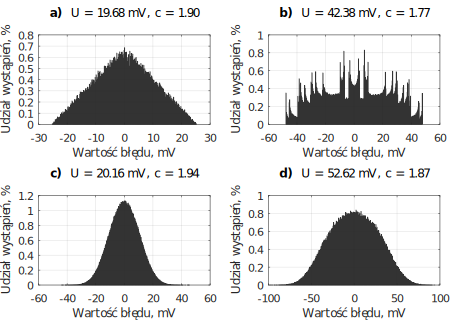
\includegraphics{obrazki/hist_part_b}
\DIFdelbeginFL %DIFDELCMD < \makecaption{fig:symul_partb_hist}{Histogramy realizacji sygnałów błędów \textbf{a)}~statycznego, \textbf{b)}~dynamicznego, \textbf{c)}~losowego, \textbf{d)}~wypadkowego, wielkości wyjściowej analizowanego w eksperymencie symulacyjnym wzmacniacza pomiarowego uzyskane metodą Monte-Carlo}
%DIFDELCMD < %%%
\DIFdelendFL \DIFaddbeginFL \makecaption{fig:symul_partb_hist}{Histogramy realizacji sygnałów błędów \textbf{a)}~statycznego, \textbf{b)}~dynamicznego, \textbf{c)}~losowego, \textbf{d)}~wypadkowego wielkości wyjściowej analizowanego w eksperymencie symulacyjnym wzmacniacza pomiarowego uzyskane metodą Monte-Carlo}
\DIFaddendFL \end{center}
\end{figure}

Analizując wyniki eksperymentu zauważyć można, że uzyskane wartości dla sygnałów błędów losowego oraz statycznego są zbliżone do tych przedstawionych w tabeli~\ref{tab:sym_partb_params_unc_sum}. Pozwala to zakładać, że podobnie jak w przypadku analizy właściwości przetwornika pomiarowego, przyjęty model błędów oraz stosowane zależności poprawnie określają związki pomiędzy wskazanymi \DIFdelbegin \DIFdel{błędami }\DIFdelend \DIFaddbegin \DIFadd{sygnałami błędów }\DIFaddend i umożliwiają poprawne oszacowanie ich parametrów. Na dotychczasowym etapie przeprowadzonej analizy nie wyznaczano wypadkowych parametrów sygnału błędu dynamicznego $e_{b,d}(t)$ oraz sygnału błędu wypadkowego $e_{b,\Sigma}(t)$ -- dane te, jak pokazano na obecnym przykładzie, nie są niezbędne podczas analizy kolejnych fragmentów toru pomiarowego, przy czym zostały one wyznaczone w ramach analizy poprzedniej części tego toru w celu weryfikacji zaproponowanej metody obliczeń.

\section{Analiza przetwornika analogowo-cyfrowego}

Kolejnym elementem wchodzącym w skład analizowanego toru pomiarowego jest przetwornik analogowo-cyfrowy. W eksperymencie zakłada się, że element \DIFaddbegin \DIFadd{ten }\DIFaddend jest realizowany przy użyciu~\qty{8}{\bitOwego} przetwornika wagowego\DIFdelbegin \DIFdel{o zakresie }\DIFdelend \DIFaddbegin \DIFadd{, którego dopuszczalna wartość }\DIFaddend napięcia wejściowego \DIFdelbegin \DIFdel{z przedziału $<-3;3>\unit{V}$}\DIFdelend \DIFaddbegin \DIFadd{zawiera się w przedziale $\interval{-3}{3}~\unit{V}$}\DIFaddend . Wobec powyższych liczba dostępnych wartości \DIFaddbegin \DIFadd{realizacji }\DIFaddend wielkości wyjściowej \DIFaddbegin \DIFadd{$x_{c}(i)$ }\DIFaddend tego przetwornika wynosi $N_{q} = 2^{8} = 256$, natomiast wartość kwantu jest równa $q = \frac{3 - (-3)~\unit{V}}{256} = \qty{23.44}{mV}$.
\DIFaddbegin 

\DIFaddend Zakładając, że wielkością wyjściową \DIFdelbegin \DIFdel{$x_{c}(n)$ }\DIFdelend \DIFaddbegin \DIFadd{$x_{c}(i)$ }\DIFaddend analizowanego przetwornika będzie dyskretna reprezentacja wielkości wejściowej $y_{b}(t)$ \DIFdelbegin \DIFdel{, zapisać można na podstawie }\DIFdelend \DIFaddbegin \DIFadd{wyrażona w jednostce tej wielkości, na podstawie równania~\eqref{eq:adc_qerror} oraz }\DIFaddend równań od~\eqref{eq:adc_out_ideal} do~\eqref{eq:adc_out_error} \DIFdelbegin \DIFdel{następujące zależności:
}\DIFdelend \DIFaddbegin \DIFadd{zapisać można:
}\DIFaddend \begin{gather}
\dot{x}_{c} \DIFdelbegin %DIFDELCMD < \emb{n} %%%
\DIFdelend \DIFaddbegin \emb{i} \DIFaddend = \dot{y}_{b} \DIFdelbegin %DIFDELCMD < \emb{nT_{p}} %%%
\DIFdelend \DIFaddbegin \emb{iT_{p}} \DIFaddend \label{eq:sym_partc_out_ideal}, \\
\tilde{x}_{c} \DIFdelbegin %DIFDELCMD < \emb{n} %%%
\DIFdelend \DIFaddbegin \emb{i} \DIFaddend = \tilde{y}_{b} \DIFdelbegin %DIFDELCMD < \emb{nT_{p}} %%%
\DIFdelend \DIFaddbegin \emb{iT_{p}} \DIFaddend + e\DIFdelbegin \DIFdel{_{c,q} }\DIFdelend \DIFaddbegin \DIFadd{_{c,AC,q} }\DIFaddend \left( \tilde{y}_{b} \DIFdelbegin %DIFDELCMD < \emb{nT_{p}} %%%
\DIFdelend \DIFaddbegin \emb{iT_{p}} \DIFaddend \right) = \dot{x}_{c} \DIFdelbegin %DIFDELCMD < \emb{n} %%%
\DIFdelend \DIFaddbegin \emb{i} \DIFaddend + e_{c,\Sigma} \DIFdelbegin %DIFDELCMD < \emb{n} %%%
\DIFdelend \DIFaddbegin \emb{i} \DIFaddend \label{eq:sym_partc_out_real}, \\
e_{c,\Sigma} \DIFdelbegin %DIFDELCMD < \emb{n} %%%
\DIFdel{= }\DIFdelend \DIFaddbegin \emb{i} \DIFadd{\cong }\DIFaddend e_{b,\Sigma} \DIFdelbegin %DIFDELCMD < \emb{nT_{p}} %%%
\DIFdelend \DIFaddbegin \emb{iT_{p}} \DIFaddend + e\DIFdelbegin \DIFdel{_{c,q} }%DIFDELCMD < \left( \tilde{y}%%%
\DIFdel{_{b} }%DIFDELCMD < \emb{nT_{p}} \right) %%%
\DIFdelend \DIFaddbegin \DIFadd{_{c,rw,q} }\emb{i} \DIFaddend \label{eq:sym_partc_error_sum},
\end{gather}
gdzie $T_{p} = \frac{1}{f_{p}} = \qty{20.8(3)}{\micro s}$ jest okresem próbkowania. Na podstawie zależności danych równaniami od~\eqref{eq:adc_function} do~\eqref{eq:adc_qerrrange} zapisać można nierówność określającą przedział, w jakim znajdować się mogą wartości realizacji sygnału błędu kwantowania \DIFdelbegin \DIFdel{$e_{c,q}(x)$ jako:
}\DIFdelend \DIFaddbegin \DIFadd{$e_{c,rw,q}(i)$ jako:
}\DIFaddend \begin{equation}
\qty{-11.72}{mV} \le e\DIFdelbegin \DIFdel{_{c,q} }%DIFDELCMD < \emb{x} %%%
\DIFdelend \DIFaddbegin \DIFadd{_{c,rw,q} }\emb{i} \DIFaddend \le \qty{11.72}{mV} \label{eq:sym_partc_error_quant}.
\end{equation}
\DIFdelbegin %DIFDELCMD < 

%DIFDELCMD < %%%
\DIFdelend Analizując równanie~\eqref{eq:sym_partc_out_real} zauważyć można, że \DIFdelbegin \DIFdel{realizacja }\DIFdelend \DIFaddbegin \DIFadd{rzeczywiste wartości realizacji }\DIFaddend błędu kwantowania \DIFdelbegin \DIFdel{zależna jest }\DIFdelend \DIFaddbegin \DIFadd{$e_{AC,c,q}(x)$ zależne są }\DIFaddend od wartości \DIFdelbegin \DIFdel{przetwarzanej }\DIFdelend \DIFaddbegin \DIFadd{realizacji }\DIFaddend wielkości wejściowej \DIFdelbegin \DIFdel{analizowanego przetwornika}\DIFdelend \DIFaddbegin \DIFadd{$y_{b}(t)$}\DIFaddend . Jednakże, jak wykazano w pracach~\cite{sienkowski_kwant, sienkowski_adc}, zależność tą można pominąć. Przy założeniu, że uzyskanie na wejściu przetwornika dowolnej wartości z zakresu wartości wielkości wejściowej jest jednakowo prawdopodobne oraz że podczas pomiaru wielkość ta będzie się zmieniać, błąd kwantowania \DIFdelbegin \DIFdel{$e_{c,q}(x)$ }\DIFdelend \DIFaddbegin \DIFadd{oznaczony jako $e_{c,rw,q}(i)$ }\DIFaddend rozpatrywać można w kategoriach probabilistycznych\DIFaddbegin \DIFadd{, }\DIFaddend jako losową realizację wielkości z zakresu opisanego \DIFdelbegin \DIFdel{równaniem}\DIFdelend \DIFaddbegin \DIFadd{nierównością}\DIFaddend ~\eqref{eq:sym_partc_error_quant} o rozkładzie jednostajnym~\cite{jakubiec_system}. \DIFdelbegin \DIFdel{Takie podejście }\DIFdelend \DIFaddbegin \DIFadd{Podejście to }\DIFaddend umożliwia zastosowanie zaproponowanego w pracy modelu błędów, \DIFdelbegin \DIFdel{podczas gdy }\DIFdelend \DIFaddbegin \DIFadd{gdzie }\DIFaddend analiza zakładająca funkcję przetwarzania \DIFdelbegin \DIFdel{omawianego obiektu }\DIFdelend daną w postaci równania~\eqref{eq:adc_output} byłaby \DIFdelbegin \DIFdel{skomplikowana. Wobec powyższych założeń wariancja }\DIFdelend \DIFaddbegin \DIFadd{niemożliwa. Wariancja }\DIFaddend $\sigma_{c,rw,q}^{2}$ oraz niepewność rozszerzona $U_{c,rw,q}$\DIFaddbegin \DIFadd{, }\DIFaddend związane z \DIFdelbegin \DIFdel{błędem kwantowania $e_{c,q}(x)$ mogą być opisane w postaci}\DIFdelend \DIFaddbegin \DIFadd{sygnałem $e_{c,rw,q}(i)$, wynoszą}\DIFaddend :
\begin{gather}
\sigma_{c,rw,q}^{2} = \frac{ q^{2}}{12} = \frac{\emb{\num{23.44e-3}}^{2} }{12} = \qty{45.78}{\micro V} \label{eq:sym_partc_var_quant}, \\
U_{c,rw,q} = c_{u} \sigma_{c,rw,q} = \num{1.65} \cdot \num{6.77e-3} = \qty{11.16}{mV} \label{eq:sym_partc_uncert_quant},
\end{gather}
gdzie zgodnie z założeniami opisanymi w~\cite{gray_quantization, widrow_quantization} przyjmuje się model błędu kwantowania zbliżony do modelu addytywnego szumu o stałej widmowej gęstości mocy i jednakowym prawdopodobieństwie uzyskania każdej z możliwych realizacji tego błędu.

Aby zweryfikować poprawność przedstawionych zależności przeprowadzono eksperyment stosując metodę Monte-Carlo. W ramach eksperymentu~\num{100000} razy wyznaczono wartość realizacji wielkości wyjściowej analizowanego obiektu, a następnie porównano ją z wartością idealną, uzyskaną dla fragmentu toru pomiarowego w którym nie występowały żadne źródła błędów. Działanie analizowanego przetwornika opisane było równaniem zgodnym z zależnością~\eqref{eq:adc_output}. Na podstawie uzyskanych zgodnie z równaniem~\DIFdelbegin \DIFdel{\eqref{eq:sym_partc_error_sum} }\DIFdelend \DIFaddbegin \DIFadd{\eqref{eq:sym_partc_out_real} }\DIFaddend wartości realizacji sygnału błędu wyznaczono wariancję tego sygnału oraz niepewność rozszerzoną na podstawie równania~\eqref{eq:unc_summation}. Identyczny eksperyment przeprowadzono ponownie z tą różnicą, że jako jedyne źródło błędów uwzględniono w nim obecność procesu kwantowania w celu oszacowania parametrów sygnału błędu kwantowania. Rysunek~\ref{fig:symul_partc_hist} przedstawia uzyskane na drodze eksperymentu histogramy.

\begin{figure}[htb!]
\begin{center}
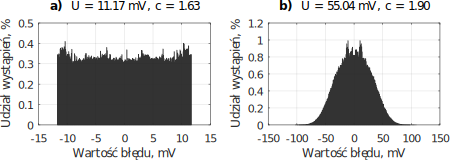
\includegraphics{obrazki/hist_part_c}
\DIFdelbeginFL %DIFDELCMD < \makecaption{fig:symul_partc_hist}{Histogramy realizacji sygnałów błędów \textbf{a)}~kwantowania, \textbf{b)}~wypadkowego, wielkości wyjściowej analizowanego w eksperymencie symulacyjnym przetwornika analogowo-cyfrowego uzyskane metodą Monte-Carlo}
%DIFDELCMD < %%%
\DIFdelendFL \DIFaddbeginFL \makecaption{fig:symul_partc_hist}{Histogramy realizacji sygnałów błędów \textbf{a)}~kwantowania, \textbf{b)}~wypadkowego wielkości wyjściowej analizowanego w eksperymencie symulacyjnym przetwornika analogowo-cyfrowego uzyskane metodą Monte-Carlo}
\DIFaddendFL \end{center}
\end{figure}

\DIFdelbegin \DIFdel{Analizując wyniki poprzedniego eksperymentu, przedstawione na rysunku~\ref{fig:symul_partb_hist} , orazwyniki bieżącego eksperymentu, przedstawione na rysunku~\ref{fig:symul_partc_hist} , wnioskować można}\DIFdelend \DIFaddbegin \DIFadd{Przedstawione na rysunkach~\ref{fig:symul_partb_hist} oraz~\ref{fig:symul_partc_hist} histogramy pozwalają stwierdzić}\DIFaddend , że przyjęte \DIFaddbegin \DIFadd{dla modelu błędu kwantowania }\DIFaddend założenia są \DIFdelbegin \DIFdel{spełnione. Wariancja }\DIFdelend \DIFaddbegin \DIFadd{poprawne. W poprzednim eksperymencie wartość wariancji $\sigma_{b,\Sigma}^{2}$ wypadkowego }\DIFaddend sygnału błędu \DIFdelbegin \DIFdel{wypadkowego $\sigma_{b,\Sigma}^{2}$ }\DIFdelend wielkości wejściowej przetwornika analogowo-cyfrowego wyniosła~\qty{788.18}{\micro V}\DIFdelbegin \DIFdel{w poprzednim eksperymencie. Wariancja }\DIFdelend \DIFaddbegin \DIFadd{. W bieżącym eksperymencie wartość wariancji $\sigma_{c,\Sigma}^{2}$ wypadkowego }\DIFaddend sygnału błędu \DIFdelbegin \DIFdel{wypadkowego $\sigma_{c,\Sigma}^{2}$ }\DIFdelend wielkości wyjściowej \DIFdelbegin \DIFdel{przetwornika analogowo-cyfrowego }\DIFdelend \DIFaddbegin \DIFadd{tego przetwornika }\DIFaddend wyniosła\DIFdelbegin \DIFdel{w bieżącym eksperymencie}\DIFdelend ~\qty{835.18}{\micro V}\DIFdelbegin \DIFdel{, }\DIFdelend \DIFaddbegin \DIFadd{. Oszacowana }\DIFaddend wartość wariancji \DIFaddbegin \DIFadd{$\sigma_{c,AC,q}^{2}$ sygnału }\DIFaddend błędu kwantowania \DIFdelbegin \DIFdel{$\sigma_{c,rw,q}^{2}$ }\DIFdelend \DIFaddbegin \DIFadd{dla założenia $\tilde{y}_{b}(i) = \dot{y}_{b}(i)$ }\DIFaddend wyniosła~\qty{46.88}{\micro V}, \DIFdelbegin \DIFdel{natomiast }\DIFdelend \DIFaddbegin \DIFadd{a }\DIFaddend związana z nią niepewność rozszerzona \DIFdelbegin \DIFdel{$U_{c,rw,q}$ }\DIFdelend wyniosła~\qty{11.16}{mV}. Uzyskane wartości pokrywają się z \DIFdelbegin \DIFdel{wartościami }\DIFdelend \DIFaddbegin \DIFadd{tymi }\DIFaddend wyznaczonymi na podstawie równań~\eqref{eq:sym_partc_var_quant} oraz~\eqref{eq:sym_partc_uncert_quant} \DIFaddbegin \DIFadd{dla modelu błędu kwantowania $e_{c,rw,q}(i)$}\DIFaddend . Korelację pomiędzy \DIFaddbegin \DIFadd{wypadkowym }\DIFaddend sygnałem błędu \DIFdelbegin \DIFdel{wypadkowego $e_{b,\Sigma}(t)$ }\DIFdelend \DIFaddbegin \DIFadd{$e_{c,\Sigma}(i)$ }\DIFaddend wielkości wejściowej \DIFdelbegin \DIFdel{przetwornika analogowo-cyfrowego oraz }\DIFdelend \DIFaddbegin \DIFadd{analizowanego przetwornika oraz rzeczywistym }\DIFaddend sygnałem błędu kwantowania \DIFdelbegin \DIFdel{$e_{c,rw,q}(n)$ }\DIFdelend \DIFaddbegin \DIFadd{$e_{c,AC,q}(x)$ }\DIFaddend określić można na podstawie równania~\eqref{eq:var_corr}, przy czym \DIFdelbegin \DIFdel{:
}\DIFdelend \DIFaddbegin \DIFadd{jej wartość wynosi:
}\DIFaddend \begin{equation}
r\DIFdelbegin \DIFdel{_{c,rw,q;b,\Sigma} = \frac{\sigma_{c,\Sigma}^{2} - \sigma_{c,rw,q}^{2} - \sigma_{b,\Sigma}^{2}}{2 \sigma_{c,rw,q} \sigma_{b,\Sigma}} }\DIFdelend \DIFaddbegin \DIFadd{_{c,AC,q;b,\Sigma} }\DIFaddend = \DIFdelbegin \DIFdel{\frac{\num{8.4e-4} - \num{4.7e-5} - \num{7.9e-4}}{2 \cdot \num{6.85e-3} \cdot \num{2.81e-2}} }\DIFdelend \DIFaddbegin \DIFadd{\frac{\sigma_{c,\Sigma}^{2} - \sigma_{c,AC,q}^{2} - \sigma_{b,\Sigma}^{2}}{2 \sigma_{c,AC,q} \sigma_{b,\Sigma}} }\DIFaddend = \num{7.8e-4} \label{eq:sym_partc_corr}.
\end{equation}
\DIFdelbegin \DIFdel{Uzyskana wartość współczynnika korelacji oraz wyniki przeprowadzonych eksperymentów świadczą o prawidłowości przyjętych założeń. Wobec powyższych założyć można, }\DIFdelend \DIFaddbegin \DIFadd{Jako, }\DIFaddend że \DIFdelbegin \DIFdel{przetwarzane przez analizowany obiekt }\DIFdelend \DIFaddbegin \DIFadd{omawiana korelacja jest pomijalnie mała, zasadne jest przyjęcie założenia braku korelacji sygnałów $e_{c,rw,q}(i)$ oraz $e_{b,\Sigma}(t)$, wobec którego $r_{c,rw,q;b,\Sigma} = 0$. Zgodnie z założeniami~\eqref{eq:adc_varout} oraz~\eqref{eq:adc_errout} przedstawić można zatem następujące relacje:
}\begin{gather}
\DIFadd{e_{c} \emb{i} \cong e_{b} \emb{iT_{p}} \label{eq:sym_partc_err_prop}, }\\
\DIFadd{\sigma_{c}^{2} \emb{\omega} \cong \sigma_{b}^{2} \emb{\omega} \label{eq:sym_partc_var_prop},
}\end{gather}
\DIFadd{opisujące }\DIFaddend sygnały błędów \DIFdelbegin \DIFdel{przenoszone będą na jego wyjście zgodnie z zależnością:
}\begin{eqnarray*}
\DIFdel{e_{c} \emb{n} \cong e_{b} \emb{nT_{p}} \label{eq:sym_partc_err_prop}, }\\
\DIFdel{\sigma_{c}^{2} \emb{\omega} \cong \sigma_{b}^{2} \emb{\omega} \label{eq:sym_partc_var_prop},
}\end{eqnarray*}%DIFAUXCMD
\DIFdel{a zatem zachowają one swoje oryginalne parametry}\DIFdelend \DIFaddbegin \DIFadd{na wyjściu analizowanego obiektu i związane z nimi wariancje}\DIFaddend . Na podstawie przedstawionych \DIFaddbegin \DIFadd{dotychczas }\DIFaddend zależności oraz \DIFaddbegin \DIFadd{danych zawartych w }\DIFaddend tabeli~\ref{tab:sym_partb_params_unc_list} sporządzono budżet niepewności wielkości wyjściowej \DIFdelbegin \DIFdel{$x_{c}(n)$ }\DIFdelend \DIFaddbegin \DIFadd{$x_{c}(i)$ }\DIFaddend analizowanego przetwornika analogowo-cyfrowego, który zestawiono w tabeli~\ref{tab:sym_partc_params_unc_list}.

\DIFdelbegin %DIFDELCMD < \begin{table}[htb!]
%DIFDELCMD < \begin{center}
%DIFDELCMD < \makecaption{tab:sym_partc_params_unc_list}{Budżet niepewności wielkości wyjściowej analizowanego w eksperymencie symulacyjnym przetwornika analogowo-cyfrowego, gdzie (a) oznacza przetwornik pomiarowy, (b) oznacza wzmacniacz pomiarowy oraz (c) oznacza przetwornik analogowo-cyfrowy}
%DIFDELCMD < \begin{tabular}[c]{| c | c | S[table-format = 2.2] | S[table-format = 3.2] | c | c |} \hline
%DIFDELCMD < \textbf{Lp.} & \textbf{Symbol} & \textbf{$U$, mV} & \textbf{$\sigma^{2}$, \micro V} & \textbf{Rozkład} & \textbf{Źródło błędu} \\ \hline
%DIFDELCMD < 1  & ${c,rw,q}$     & 11.16 &  45.78  & jednostajny                  & proces kwantowania (c)                     \\ \hline
%DIFDELCMD < 2  & ${c,sp,1}$     & 11.52 &  36.75  & trójkątny                    & dryft temperatury (a)                       \\ \hline
%DIFDELCMD < 3  & ${c,sp,2}$     & 8.15  &  18.38  & trójkątny                    & dryft temperatury (b)                       \\ \hline
%DIFDELCMD < 4  & ${c,rp,1}$     & 9.93  &  36.26  & jednostajny                  & nieliniowość obiektu (a)                   \\ \hline
%DIFDELCMD < 5  & ${c,rp,2}$     & 16.70 &  72.64  & normalny                     & szum wielkości wejściowej                  \\ \hline
%DIFDELCMD < 6  & ${c,dp,a,1}$   & 6.21  &  19.14  & \multirow{6}{*}{dwumodalny}  & \multirow{3}{*}{transmitancja (a)}         \\ \cline{1-4}
%DIFDELCMD < 7  & ${c,dp,a,2}$   & 15.53 &  119.62 &                              &                                            \\ \cline{1-4}
%DIFDELCMD < 8  & ${c,dp,a,3}$   & 15.52 &  119.44 &                              &                                            \\ \cline{1-4} \cline{6-6}
%DIFDELCMD < 9  & ${c,dp,b,1}$   & 3.06  &  4.64   &                              & \multirow{3}{*}{transmitancja (b)}         \\ \cline{1-4}
%DIFDELCMD < 10 & ${c,dp,b,2}$   & 7.65  &  29.00  &                              &                                            \\ \cline{1-4}
%DIFDELCMD < 11 & ${c,dp,b,3}$   & 7.65  &  28.99  &                              &                                            \\ \hline
%DIFDELCMD < \end{tabular}
%DIFDELCMD < \end{center}
%DIFDELCMD < \end{table}
%DIFDELCMD < %%%
\DIFdelend \DIFaddbegin \begin{table}[htb!]
\begin{center}
\makecaption{tab:sym_partc_params_unc_list}{Budżet niepewności wielkości wyjściowej analizowanego w eksperymencie symulacyjnym przetwornika analogowo-cyfrowego, gdzie ($a$) oznacza przetwornik pomiarowy, ($b$) oznacza wzmacniacz pomiarowy oraz ($c$) oznacza przetwornik analogowo-cyfrowy}
\begin{tabular}[c]{| c | c | S[table-format = 2.2] | S[table-format = 3.2] | c | c |} \hline
\textbf{Lp.} & \textbf{Symbol} & \textbf{$U$, mV} & \textbf{$\sigma^{2}$, \micro V} & \textbf{Rozkład} & \textbf{Źródło błędu} \\ \hline
1  & ${c,rw,q}$     & 11.16 &  45.78  & jednostajny                  & proces kwantowania ($c$)                   \\ \hline
2  & ${c,sp,1}$     & 11.52 &  36.75  & trójkątny                    & dryft temperatury ($a$)                    \\ \hline
3  & ${c,sp,2}$     & 8.15  &  18.38  & trójkątny                    & dryft temperatury ($b$)                    \\ \hline
4  & ${c,rp,1}$     & 9.93  &  36.26  & jednostajny                  & nieliniowość obiektu ($a$)                 \\ \hline
5  & ${c,rp,2}$     & 16.70 &  72.64  & normalny                     & szum wielkości wejściowej                  \\ \hline
6  & ${c,dp,a,1}$   & 6.21  &  19.14  & \multirow{6}{*}{dwumodalny}  & \multirow{3}{*}{transmitancja ($a$)}       \\ \cline{1-4}
7  & ${c,dp,a,2}$   & 15.53 &  119.62 &                              &                                            \\ \cline{1-4}
8  & ${c,dp,a,3}$   & 15.52 &  119.44 &                              &                                            \\ \cline{1-4} \cline{6-6}
9  & ${c,dp,b,1}$   & 3.06  &  4.64   &                              & \multirow{3}{*}{transmitancja ($b$)}       \\ \cline{1-4}
10 & ${c,dp,b,2}$   & 7.65  &  29.00  &                              &                                            \\ \cline{1-4}
11 & ${c,dp,b,3}$   & 7.65  &  28.99  &                              &                                            \\ \hline
\end{tabular}
\end{center}
\end{table}
\DIFaddend 

Przedstawiony w tabeli~\ref{tab:sym_partc_params_unc_list} budżet niepewności dobrze obrazuje źródła sygnałów błędów występujące w analizowanym torze pomiarowym oraz jednoznacznie wskazuje ich parametry. Na dalszym etapie analizy stosowanie przedstawionego zestawienia jest jednak kłopotliwe, ponieważ wiąże się z koniecznością analizy każdego ze wskazanych sygnałów \DIFdelbegin \DIFdel{błędu }\DIFdelend \DIFaddbegin \DIFadd{błędów }\DIFaddend z osobna. Ze względu na fakt, że proponowany w pracy model błędów dotyczący kolejnego fragmentu toru pomiarowego, jakim jest algorytm transformacji falkowej, wymaga jedynie określenia parametrów \DIFdelbegin \DIFdel{wypadkowego sygnału błędu statycznego , }\DIFdelend \DIFaddbegin \DIFadd{wypadkowych sygnałów błędów statycznego i }\DIFaddend losowego oraz wypadkowych parametrów kolejnych harmonicznych sygnału błędu dynamicznego, proponuje się sporządzenie budżetu niepewności uwzględniającego opisywany podział, podobnie jak to miało miejsce w przypadku poprzedniego elementu analizowanego toru pomiarowego.

Parametry opisujące wypadkowy sygnał błędu losowego wyznaczyć można zgodnie z równaniami~\eqref{eq:var_sum} oraz~\eqref{eq:unc_matrix}, które w obecnym przypadku przyjmują postać:
\begin{gather}
\sigma_{c,r}^{2} = \sigma_{c,rp,1}^{2} + \sigma_{c,rp,2}^{2} + \sigma\DIFdelbegin \DIFdel{_{c,q}}\DIFdelend \DIFaddbegin \DIFadd{_{c,rw,q}}\DIFaddend ^{2} = \sigma_{b,rp,1}^{2} + \sigma_{b,rp,2}^{2} + \sigma\DIFdelbegin \DIFdel{_{c,q}}\DIFdelend \DIFaddbegin \DIFadd{_{c,rw,q}}\DIFaddend ^{2} = \qty{154.68}{\micro V} \label{eq:sym_partc_rand_var}, \\
\DIFdelbegin %DIFDELCMD < \begin{split}
%DIFDELCMD < U_{c,r} = ~ & \sqrt{
%DIFDELCMD < \begin{bmatrix}
%DIFDELCMD < U_{c,rp,1} \\ U_{c,rp,2} \\ U_{c,q}
%DIFDELCMD < \end{bmatrix}^{T}
%DIFDELCMD < \begin{bmatrix}
%DIFDELCMD < 1            & h_{c,rp,1,2} & h_{c,rp,1,q} \\
%DIFDELCMD < h_{c,rp,2,1} & 1            & h_{c,rp,2,q} \\
%DIFDELCMD < h_{c,q,rp,1} & h_{c,q,rp,2} & 1
%DIFDELCMD < \end{bmatrix}
%DIFDELCMD < \begin{bmatrix}
%DIFDELCMD < U_{c,rp,1} \\ U_{c,rp,2} \\ U_{c,q}
%DIFDELCMD < \end{bmatrix}} = ~ \\ & \sqrt{
%DIFDELCMD < \begin{bmatrix}
%DIFDELCMD < \num{9.93e-3} \\ \num{16.70e-3} \\ \num{11.16e-3}
%DIFDELCMD < \end{bmatrix}^{T}
%DIFDELCMD < \begin{bmatrix}
%DIFDELCMD < \num{1.000} & \num{0.091} & \num{0.141} \\
%DIFDELCMD < \num{0.091} & \num{1.000} & \num{0.103} \\
%DIFDELCMD < \num{0.141} & \num{0.103} & \num{1.000}
%DIFDELCMD < \end{bmatrix}
%DIFDELCMD < \begin{bmatrix}
%DIFDELCMD < \num{9.93e-3} \\ \num{16.70e-3} \\ \num{11.16e-3}
%DIFDELCMD < \end{bmatrix}} = \qty{24.53}{mV}
%DIFDELCMD < \end{split}%%%
\DIFdelend \DIFaddbegin \begin{split}
U_{c,r} = ~ & \sqrt{
\begin{bmatrix}
U_{c,rp,1} \\ U_{c,rp,2} \\ U_{c,rw,q}
\end{bmatrix}^{T}
\begin{bmatrix}
1               & h_{c,rp,1,2}    & h_{c,rp,1,rw,q} \\
h_{c,rp,2,1}    & 1               & h_{c,rp,2,rw,q} \\
h_{c,rw,q,rp,1} & h_{c,rw,q,rp,2} & 1
\end{bmatrix}
\begin{bmatrix}
U_{c,rp,1} \\ U_{c,rp,2} \\ U_{c,rw,q}
\end{bmatrix}} = ~ \\ & \sqrt{
\begin{bmatrix}
\num{9.93e-3} \\ \num{16.70e-3} \\ \num{11.16e-3}
\end{bmatrix}^{T}
\begin{bmatrix}
\num{1.000} & \num{0.091} & \num{0.141} \\
\num{0.091} & \num{1.000} & \num{0.103} \\
\num{0.141} & \num{0.103} & \num{1.000}
\end{bmatrix}
\begin{bmatrix}
\num{9.93e-3} \\ \num{16.70e-3} \\ \num{11.16e-3}
\end{bmatrix}} = \qty{24.53}{mV}
\end{split}\DIFaddend 
\label{eq:sym_partc_rand_uncert}, \\
h_{c,rp,1,2} = s_{u,n} \sqrt{\frac{\num{9.93e-3}}{\num{16.70e-3}}} \left( \frac{\num{98.60e-6} + \num{278.89e-6}}{\num{502.04e-6}} \right) = \num{0.091} \label{eq:sym_partc_coher_rp_1_2}, \\
h\DIFdelbegin \DIFdel{_{c,q,rp,1} }\DIFdelend \DIFaddbegin \DIFadd{_{c,rw,q,rp,1} }\DIFaddend = s_{u,u} \sqrt{\frac{\num{9.93e-3}}{\num{11.16e-3}}} \left( \frac{\num{98.60e-6} + \num{124.55e-6}}{\num{502.04e-6}} \right) = \num{0.141} \label{eq:sym_partc_coher_q_rp_1}, \\
h\DIFdelbegin \DIFdel{_{c,q,rp,2} }\DIFdelend \DIFaddbegin \DIFadd{_{c,rw,q,rp,2} }\DIFaddend = s_{u,n} \sqrt{\frac{\num{11.16e-3}}{\num{16.70e-3}}} \left( \frac{\num{124.55e-6} + \num{278.89e-6}}{\num{502.04e-6}} \right) = \num{0.103} \label{eq:sym_partc_coher_q_rp_2}, \\
c_{c,r} = \frac{U_{c,r}}{\sigma_{c,r}} = \frac{\num{24.53e-3}}{\num{12.44e-3}} = \num{1.97} \label{eq:sym_partc_rand_factor}.
\end{gather}

Na podstawie wyznaczonej w równaniu~\eqref{eq:sym_partc_rand_factor} wartości współczynnika rozszerzenia oraz ze względu na spełnienie w analizowanym przypadku warunków centralnego twierdzenia granicznego, zakładać można normalny rozkład wypadkowego sygnału błędu losowego. Biorąc pod uwagę przedstawione dotychczas założenia, wyniki zawarte w tabelach~\ref{tab:sym_partb_params_unc_sum} oraz~\ref{tab:sym_partc_params_unc_list}, jak również wyniki obliczeń przedstawionych w równaniach~\eqref{eq:sym_partc_rand_var} oraz~\eqref{eq:sym_partc_rand_uncert}, sporządzono budżet niepewności z uwzględnieniem omawianego wcześniej podziału, który zestawiono w tabeli~\ref{tab:sym_partc_params_unc_sum}.

\begin{table}[htb!]
\begin{center}
\makecaption{tab:sym_partc_params_unc_sum}{Budżet niepewności wielkości wyjściowej analizowanego w eksperymencie symulacyjnym przetwornika analogowo-cyfrowego z uwzględnieniem podziału na wypadkowe sygnały błędów statycznych, dynamicznych oraz losowych}
\begin{tabular}[c]{| c | c | S[table-format = 2.2] | S[table-format = 3.2] | c | c |} \hline
\textbf{Lp.} & \textbf{Symbol} & \textbf{$U$, mV} & \textbf{$\sigma^{2}$, \micro V} & \textbf{Rozkład} & \textbf{Źródło błędu} \\ \hline
1 & ${c,s}$        & 19.67 &  107.12 & trójkątny                    & wypadkowy dryft temperatury                \\ \hline
2 & ${c,r}$        & 24.53 &  154.68 & normalny                     & szum, nieliniowość, konwersja              \\ \hline
3 & ${c,d,1}$      & 9.20  &  42.60  & \multirow{3}{*}{dwumodalny}  & \multirow{3}{*}{wypadkowa transmitancja}   \\ \cline{1-4}
4 & ${c,d,2}$      & 23.01 &  266.34 &                              &                                            \\ \cline{1-4}
5 & ${c,d,3}$      & 23.00 &  266.11 &                              &                                            \\ \hline
\end{tabular}
\end{center}
\end{table}

\section{Analiza algorytmu transformacji falkowej}

Ostatnim, przy czym najistotniejszym z punktu widzenia pracy, fragmentem analizowanego toru pomiarowego jest algorytm dyskretnej transformacji falkowej. Zakłada się, że dla każdej $k$-tej realizacji pomiaru na wejście algorytmu podawany jest wektor wielkości wejściowych $\mathbf{x}_{d}(k)$ złożony z $N = 8$ występujących po sobie próbek wielkości wyjściowej $x_{c}(i)$ przetwornika analogowo-cyfrowego. Wyjście analizowanego algorytmu stanowi wektor $\mathbf{X}(k)$ składający się z $M = 8$ wielkości, które stanowią ostateczne wielkości wyjściowe analizowanego toru pomiarowego. Omawiany algorytm wykorzystuje falkę \enquote{db2}, przy czym na jego realizację składają się dwie iteracje procesu dekompozycji sygnału. Macierz transformacji $\mathbf{A}$ omawianego algorytmu przedstawia równanie~\eqref{eq:db2_2_8_matrix}. Zakłada się, że implementacja stosowanego algorytmu wykorzystuje liczby zmiennoprzecinkowe połowicznej precyzji, o długości słowa~\qty{16}{\bitOw}~\cite{gcc_manual}.

Wobec powyższych założeń oraz modelu zaproponowanego w równaniach od~\eqref{eq:alg_out_mat} do~\eqref{eq:alg_out_single} wektor wielkości wejściowych analizowanego algorytmu opisać można w postaci:
\begin{gather}
\dot{\mathbf{x}}_{d}^{T} \emb{k} =
\DIFdelbegin %DIFDELCMD < \begin{bmatrix}
%DIFDELCMD < \dot{x}_{c} \emb{kT_{p}} & \dot{x}_{c} \left( \emb{k+1} T_{p} \right) & \hdots & \dot{x}_{c} \left( \emb{k+7} T_{p} \right)
%DIFDELCMD < \end{bmatrix}%%%
\DIFdelend \DIFaddbegin \begin{bmatrix}
\dot{x}_{c} \emb{kNT_{p}} & \dot{x}_{c} \left( \emb{kN+1} T_{p} \right) & \hdots & \dot{x}_{c} \left( \emb{kN+7} T_{p} \right)
\end{bmatrix}\DIFaddend 
\label{eq:sym_partd_input_ideal}, \\
\tilde{\mathbf{x}}_{d}^{T} \emb{k} =
\DIFdelbegin %DIFDELCMD < \begin{bmatrix}
%DIFDELCMD < \tilde{x}_{c} \emb{kT_{p}} & \tilde{x}_{c} \left( \emb{k+1} T_{p} \right) & \hdots & \tilde{x}_{c} \left( \emb{k+7} T_{p} \right)
%DIFDELCMD < \end{bmatrix}%%%
\DIFdelend \DIFaddbegin \begin{bmatrix}
\tilde{x}_{c} \emb{kNT_{p}} & \tilde{x}_{c} \left( \emb{kN+1} T_{p} \right) & \hdots & \tilde{x}_{c} \left( \emb{kN+7} T_{p} \right)
\end{bmatrix}\DIFaddend 
\label{eq:sym_partd_input_real}\DIFdelbegin \DIFdel{.
}\DIFdelend \DIFaddbegin \DIFadd{,
}\DIFaddend \end{gather}
\DIFdelbegin \DIFdel{Wektor realizacji sygnału błędu }\DIFdelend \DIFaddbegin \DIFadd{zatem wektor sygnałów błędów }\DIFaddend wielkości wyjściowych \DIFdelbegin \DIFdel{algorytmu opisuje równanie:
}\DIFdelend \DIFaddbegin \DIFadd{może być zdefiniowany jako:
}\DIFaddend \begin{equation}
\mathbf{e}_{d,\Sigma}^{T} \emb{k} =
\DIFdelbegin %DIFDELCMD < \begin{bmatrix}
%DIFDELCMD < e_{c,\Sigma} \emb{kT_{p}} & e_{c,\Sigma} \left( \emb{k+1} T_{p} \right) & \hdots & e_{c,\Sigma} \left( \emb{k+7} T_{p} \right)
%DIFDELCMD < \end{bmatrix}%%%
\DIFdelend \DIFaddbegin \begin{bmatrix}
e_{c,\Sigma} \emb{kMT_{p}} & e_{c,\Sigma} \left( \emb{kM+1} T_{p} \right) & \hdots & e_{c,\Sigma} \left( \emb{kM+7} T_{p} \right)
\end{bmatrix}\DIFaddend 
\label{eq:sym_partd_input_error_sum}.
\end{equation}
Dodatkowo zdefiniować można \DIFdelbegin \DIFdel{wektory realizacji }\DIFdelend \DIFaddbegin \DIFadd{kolejne wektory }\DIFaddend sygnałów błędów\DIFaddbegin \DIFadd{, }\DIFaddend rozpatrując zaproponowany podział na błędy statyczne, losowe oraz dynamiczne\DIFdelbegin \DIFdel{:
}\DIFdelend \DIFaddbegin \DIFadd{, gdzie:
}\DIFaddend \begin{gather}
\mathbf{e}_{d,s}^{T} \emb{k} =
\DIFdelbegin %DIFDELCMD < \begin{bmatrix}
%DIFDELCMD < e_{c,s} \emb{kT_{p}} & e_{c,s} \left( \emb{k+1} T_{p} \right) & \hdots & e_{c,s} \left( \emb{k+7} T_{p} \right)
%DIFDELCMD < \end{bmatrix}%%%
\DIFdelend \DIFaddbegin \begin{bmatrix}
e_{c,s} \emb{kMT_{p}} & e_{c,s} \left( \emb{kM+1} T_{p} \right) & \hdots & e_{c,s} \left( \emb{kM+7} T_{p} \right)
\end{bmatrix}\DIFaddend 
\label{eq:sym_partd_input_error_stat}, \\
\mathbf{e}_{d,r}^{T} \emb{k} =
\DIFdelbegin %DIFDELCMD < \begin{bmatrix}
%DIFDELCMD < e_{c,r} \emb{kT_{p}} & e_{c,r} \left( \emb{k+1} T_{p} \right) & \hdots & e_{c,r} \left( \emb{k+7} T_{p} \right)
%DIFDELCMD < \end{bmatrix}%%%
\DIFdelend \DIFaddbegin \begin{bmatrix}
e_{c,r} \emb{kMT_{p}} & e_{c,r} \left( \emb{kM+1} T_{p} \right) & \hdots & e_{c,r} \left( \emb{kM+7} T_{p} \right)
\end{bmatrix}\DIFaddend 
\label{eq:sym_partd_input_error_rand}, \\
\mathbf{e}_{d,d}^{T} \emb{k} =
\DIFdelbegin %DIFDELCMD < \begin{bmatrix}
%DIFDELCMD < e_{c,d} \emb{kT_{p}} & e_{c,d} \left( \emb{k+1} T_{p} \right) & \hdots & e_{c,d} \left( \emb{k+7} T_{p} \right)
%DIFDELCMD < \end{bmatrix}%%%
\DIFdelend \DIFaddbegin \begin{bmatrix}
e_{c,d} \emb{kMT_{p}} & e_{c,d} \left( \emb{kM+1} T_{p} \right) & \hdots & e_{c,d} \left( \emb{kM+7} T_{p} \right)
\end{bmatrix}\DIFaddend 
\label{eq:sym_partd_input_error_dyn},
\end{gather}
\DIFdelbegin \DIFdel{a także }\DIFdelend \DIFaddbegin \DIFadd{przy czym }\DIFaddend w analogiczny sposób rozpatrywać można wektory sygnałów błędów cząstkowych, których parametry zestawiono w tabeli~\ref{tab:sym_partc_params_unc_list}. Wobec powyższego, zgodnie z równaniem~\eqref{eq:alg_out_mul}, wektor wielkości wyjściowych opisać można jako:
\begin{gather}
\dot{\mathbf{X}} \emb{k} = \mathbf{A} \cdot \dot{\mathbf{x}}_{d} \emb{k} \label{eq:sym_partd_output_ideal}, \\
\tilde{\mathbf{X}} \emb{k} = \mathbf{A} \cdot \tilde{\mathbf{x}}_{d} \emb{k} + \mathbf{e}_{d,z} \emb{k} = \dot{\mathbf{X}} \emb{k} + \mathbf{e}_{X,\Sigma} \emb{k} \label{eq:sym_partd_output_real},
\end{gather}
gdzie $\mathbf{e}_{d,z}(k)$ jest wektorem \DIFdelbegin \DIFdel{realizacji błędu własnego }\DIFdelend \DIFaddbegin \DIFadd{sygnałów błędów własnych }\DIFaddend zaokrągleń\DIFdelbegin \DIFdel{$e_{d,z}(j)$}\DIFdelend , natomiast kolejne wektory \DIFdelbegin \DIFdel{realizacji }\DIFdelend sygnałów błędów wielkości wyjściowej są opisane w postaci:
\begin{gather}
\mathbf{e}_{X,\Sigma} \emb{k} = \mathbf{A} \cdot \mathbf{e}_{d,\Sigma} \emb{k} = \mathbf{e}_{X,s} \emb{k} + \mathbf{e}_{X,d} \emb{k} + \mathbf{e}_{X,r} \emb{k} + \mathbf{e}_{d,z} \emb{k} \label{eq:sym_partd_output_error_sum}, \\
\mathbf{e}_{X,s} \emb{k} = \mathbf{A} \cdot \mathbf{e}_{d,s} \emb{k} \label{eq:sym_partd_output_error_stat}, \\
\mathbf{e}\DIFdelbegin \DIFdel{_{X,d} }\DIFdelend \DIFaddbegin \DIFadd{_{X,r} }\DIFaddend \emb{k} = \mathbf{A} \cdot \mathbf{e}\DIFdelbegin \DIFdel{_{d,d} }\DIFdelend \DIFaddbegin \DIFadd{_{d,r} }\DIFaddend \emb{k} \DIFdelbegin %DIFDELCMD < \label{eq:sym_partd_output_error_dyn}%%%
\DIFdelend \DIFaddbegin \label{eq:sym_partd_output_error_rand}\DIFaddend , \\
\mathbf{e}\DIFdelbegin \DIFdel{_{X,r} }\DIFdelend \DIFaddbegin \DIFadd{_{X,d} }\DIFaddend \emb{k} = \mathbf{A} \cdot \mathbf{e}\DIFdelbegin \DIFdel{_{d,r} }\DIFdelend \DIFaddbegin \DIFadd{_{d,d} }\DIFaddend \emb{k} \DIFdelbegin %DIFDELCMD < \label{eq:sym_partd_output_error_rand}%%%
\DIFdelend \DIFaddbegin \label{eq:sym_partd_output_error_dyn}\DIFaddend .
\end{gather}

Należy zauważyć, że tak jak w przypadku wektora wielkości wejściowych, tak i w przypadku wektora wielkości wyjściowych, wyróżnić można również osobne wektory realizacji sygnałów błędów dla każdego z opisanych w tabeli~\ref{tab:sym_partc_params_unc_list} sygnałów. Zgodnie z oznaczeniami przyjętymi w równaniach~\eqref{eq:db2_invect} oraz~\eqref{eq:db2_outvect}, wektory wielkości wejściowych $\mathbf{x}(k)$ i wyjściowych $\mathbf{X}(k)$ pojedynczej realizacji algorytmu dla $k$-tego okna pomiarowego są w dalszej części rozdziału oznaczane symbolami:
\begin{gather}
\mathbf{x}_{d}^{T} =
\begin{bmatrix}
S_{0,0} & S_{0,1} & S_{0,2} & S_{0,3} & S_{0,4} & S_{0,5} & S_{0,6} & S_{0,7}
\end{bmatrix}
\label{eq:sym_partd_invect}, \\
\mathbf{X}^{T} =
\begin{bmatrix}
S_{2,0} & S_{2,1} & T_{2,0} & T_{2,1} & T_{1,0} & T_{1,1} & T_{1,2} & T_{1,3}
\end{bmatrix}
\label{eq:sym_partd_outvect},
\end{gather}
natomiast wektor \DIFdelbegin \DIFdel{realizacji }\DIFdelend sygnałów błędów wielkości wyjściowej $\mathbf{e}_{X,*}(k)$ dla \DIFdelbegin \DIFdel{pojedynczej }\DIFdelend \DIFaddbegin \DIFadd{wybranej }\DIFaddend $k$-tej iteracji realizacji algorytmu jest oznaczany w postaci:
\begin{equation}
\mathbf{e}_{X,*}^{T} =
\begin{bmatrix}
e_{S_{2,0},*} & e_{S_{2,1},*} & e_{T_{2,0},*} & e_{T_{2,1},*} & e_{T_{1,0},*} & e_{T_{1,1},*} & e_{T_{1,2},*} & e_{T_{1,3},*}
\end{bmatrix}
\label{eq:sym_partd_errvect},
\end{equation}
gdzie w miejsce symbolu \enquote{$*$} umieszczany jest symbol analizowanego sygnału błędu.

W poprzednich podrozdziałach przedstawiono różne sposoby wyznaczania budżetu niepewności, uwzględniające każde źródło błędu z osobna oraz wskazujące wypadkowe parametry danego rodzaju błędu. Zabiegi te miały na celu wskazanie optymalnej drogi analizy właściwości metrologicznych z punktu widzenia projektanta toru pomiarowego, tak aby nie wykonywał on czynności nieistotnych z punktu widzenia przeprowadzanej analizy. Opisywany zabieg został również przeprowadzony w celu weryfikacji postawionej w pracy tezy, jako przy wykorzystaniu zaproponowanej metody analizy istnieje możliwość wyznaczenia jedynie zastępczych parametrów sygnałów błędów wielkości wejściowej algorytmu dyskretnej transformacji falkowej w celu oszacowania wartości niepewności na wyjściu tego algorytmu. W dalszej części rozdziału opisane zostały dwa sposoby wyznaczenia niepewności wielkości wyjściowych algorytmu. Podejście pierwsze uwzględniać będzie budżet niepewności podzielony na kategorie błędów, opisany w tabeli~\ref{tab:sym_partc_params_unc_sum}, natomiast podejście drugie przedstawi analizę z wykorzystaniem budżetu sporządzonego dla każdego sygnału błędu z osobna, który przedstawiono w tabeli~\ref{tab:sym_partc_params_unc_list}.

Istotnym faktem podczas analizy właściwości metrologicznych stosowanego algorytmu jest to, że jego wielkości wejściowe każdorazowo pochodzą z tego samego źródła. Powtarzając proces wyznaczania wartości wektora wielkości wyjściowych algorytmu wielokrotnie, wszystkie wielkości wejściowe algorytmu \DIFdelbegin \DIFdel{cechowały będą }\DIFdelend \DIFaddbegin \DIFadd{cechują }\DIFaddend te same parametry wariancji i niepewności rozszerzonej. Zjawisko to zostało omówione w poprzedniej części pracy. Ze względu na fakt, że w przypadku błędów o charakterze statycznym, wartości realizacji tych błędów nie zmieniają się w obrębie pojedynczego okna pomiarowego, do oceny wariancji wyjściowego sygnału związanego z tym rodzajem błędu \DIFdelbegin \DIFdel{stosowane będzie }\DIFdelend \DIFaddbegin \DIFadd{stosowano }\DIFaddend równanie~\eqref{eq:alg_outvar_stat}. Do określenia parametrów sygnałów błędów o charakterze dynamicznym \DIFdelbegin \DIFdel{wykorzystana zostanie transmitancja }\DIFdelend \DIFaddbegin \DIFadd{wykorzystano transmitancję odpowiednią dla }\DIFaddend pojedynczej wielkości wyjściowej algorytmu\DIFdelbegin \DIFdel{dana }\DIFdelend \DIFaddbegin \DIFadd{, daną }\DIFaddend równaniem~\eqref{eq:alg_trans_single}\DIFdelbegin \DIFdel{, natomiast w }\DIFdelend \DIFaddbegin \DIFadd{. W }\DIFaddend przypadku sygnałów błędów o charakterze losowym \DIFdelbegin \DIFdel{wykorzystywana będzie w tym celu }\DIFdelend \DIFaddbegin \DIFadd{wykorzystano }\DIFaddend zależność~\eqref{eq:alg_outvar_rand}, ze względu na stałą widmową gęstość mocy tych sygnałów w zakresie częstotliwości \DIFdelbegin \DIFdel{$\hat{f} \in~<0;\frac{1}{2} f_{p}>$. Przedstawiane }\DIFdelend \DIFaddbegin \DIFadd{$\hat{f} \in \interval{0}{\frac{1}{2} f_{p}}$. Przedstawione }\DIFaddend w dalszej części obliczenia dotyczą dwóch przykładowych wielkości wyjściowych algorytmu -- $S_{2,0}$ oraz $T_{1,0}$. Wybór \DIFdelbegin \DIFdel{przedstawionych }\DIFdelend \DIFaddbegin \DIFadd{wskazanych }\DIFaddend wielkości jest uzasadniony faktem, że \DIFdelbegin \DIFdel{jedna }\DIFdelend \DIFaddbegin \DIFadd{pierwsza }\DIFaddend z nich stanowi \DIFdelbegin \DIFdel{detale }\DIFdelend \DIFaddbegin \DIFadd{aproksymacje }\DIFaddend sygnału (jest \DIFdelbegin \DIFdel{reprezentowana przez filtr dolno-przepustowy związany z funkcją skalującą}\DIFdelend \DIFaddbegin \DIFadd{związana z filtrem dolno-przepustowym, utworzonym na bazie funkcji skalującej}\DIFaddend ), natomiast druga stanowi \DIFdelbegin \DIFdel{aproksymacje }\DIFdelend \DIFaddbegin \DIFadd{detale }\DIFaddend sygnału (jest \DIFdelbegin \DIFdel{reprezentowana przez filtr pasmowo-przepustowy związany z falką-matką). Pozostałe }\DIFdelend \DIFaddbegin \DIFadd{związana z filtrem pasmowo-przepustowym, utworzonym na bazie falki-matki). Parametry pozostałych }\DIFaddend wielkości \DIFdelbegin \DIFdel{poddano analizie w identyczny sposób}\DIFdelend \DIFaddbegin \DIFadd{wyjściowych analizowano identycznie}\DIFaddend , natomiast dla zachowania czytelności pracy \DIFdelbegin \DIFdel{obliczenia te nie zostały przedstawione}\DIFdelend \DIFaddbegin \DIFadd{nie przedstawiono przykładów obliczeń}\DIFaddend .

Błędy statyczne przenoszone są przez analizowany algorytm z wejścia na wyjście zgodnie z równaniem~\eqref{eq:alg_outerr_stat}, a zatem zgodnie z zależnością~\eqref{eq:alg_outvar_stat} może zostać wyznaczona ich wariancja, przy czym na etapie analizy dla każdej wielkości wyjściowej wyznaczana jest wartość współczynnika $A_{s}$, zgodnie z równaniem~\eqref{eq:alg_trans_stat}. W przypadku błędów losowych, przenoszonych zgodnie z zależnością~\eqref{eq:alg_outerr}\DIFaddbegin \DIFadd{, }\DIFaddend ich wariancja jest wyznaczana zgodnie z równaniem~\eqref{eq:alg_outvar_rand}\DIFdelbegin \DIFdel{i, podobnie jak w przypadku błędów statycznych, }\DIFdelend \DIFaddbegin \DIFadd{, przy czym }\DIFaddend do jej wyznaczenia stosowane są współczynniki $A_{r}$ wyznaczone zgodnie z zależnością~\eqref{eq:alg_trans_rand}. \DIFdelbegin \DIFdel{Można zatem dla rozważanych }\DIFdelend \DIFaddbegin \DIFadd{Wartości omawianych }\DIFaddend wielkości \DIFdelbegin \DIFdel{wyjściowych zapisać}\DIFdelend \DIFaddbegin \DIFadd{wynoszą w rozważanym przypadku}\DIFaddend :
\begin{gather}
A_{S_{2,0},s} = \sum _{j = 0} ^{N-1} a_{0, j} = 2 \label{eq:sym_partd_output_as_S_2_0}, \\
A_{S_{2,0},r} = \sqrt{\sum _{j = 0} ^{N-1} a_{0, j}^{2}} = 1 \label{eq:sym_partd_output_ar_S_2_0}, \\
A_{T_{1,0},s} = \sum _{j = 0} ^{N-1} a_{4, j} = 0 \label{eq:sym_partd_output_as_T_1_0}, \\
A_{T_{1,0},r} = \sqrt{\sum _{j = 0} ^{N-1} a_{4, j}^{2}} = 1 \label{eq:sym_partd_output_ar_T_1_0}.
\end{gather}
Należy zauważyć, że zgodnie z oczekiwaniami wielkość wyjściowa $T_{1,0}$ nie będzie obarczona błędem statycznym w związku z faktem, że jest ona związana z filtrem pasmowo-przepustowym. Dodatkowo zauważyć można, że dla wszystkich wielkości wyjściowych współczynnik $A_{r}$ każdorazowo będzie równy jedności, co wynika z założenia rodziny \enquote{Daubechies} odnośnie normalizacji energii~\cite{vonesch_dbbasics, wei_coiflet}.

Zgodnie z równaniem~\eqref{eq:alg_trans_single} oraz postacią macierzy $\mathbf{A}$ daną równaniem~\eqref{eq:db2_2_8_matrix}, transmitancje algorytmu związane z omawianymi wielkościami wyjściowymi w dziedzinie $\mathcal{Z}$ przedstawiają następujące równania:
\begin{gather}
\begin{split}
H_{S_{2,0}} \emb{z} = ~
& \frac{5 - \sqrt{3}}{16} + \frac{5 + \sqrt{3}}{16} z^{-1} + \frac{3 + 3 \sqrt{3}}{16} z^{-2} + \frac{5 + 3 \sqrt{3}}{16} z^{-3} + \\
& \frac{3 + \sqrt{3}}{16} z^{-4} + \frac{3 - \sqrt{3}}{16} z^{-5} + \frac{5 - 3 \sqrt{3}}{16} z^{-6} + \frac{3 - 3 \sqrt{3}}{16} z^{-7}
\end{split}
\label{eq:sym_partd_output_trans_z_S_2_0}, \\
H_{T_{1,0}} \emb{z} = \frac{1 - \sqrt{3}}{4 \sqrt{2}} - \frac{3 - \sqrt{3}}{4 \sqrt{2}} z^{-1} + \frac{3 + \sqrt{3}}{4 \sqrt{2}} z^{-2} - \frac{1 + \sqrt{3}}{4 \sqrt{2}} z^{-3} \label{eq:sym_partd_output_trans_z_T_1_0}.
\end{gather}
Podstawiając do powyższych równań założenie gdzie $z = e^{j\omega_{n}}$ otrzymuje się zależności opisujące transmitancje wybranych wierszy w funkcji pulsacji znormalizowanej~\cite{oppenheim_dsp}:
\begin{gather}
\begin{split}
G_{S_{2,0}} \emb{\omega_{n}} = ~
& \frac{5 - \sqrt{3}}{16} + \frac{5 + \sqrt{3}}{16} e^{-j\omega_{n}} + \frac{3 + 3 \sqrt{3}}{16} e^{-2j\omega_{n}} + \\
& \frac{5 + 3 \sqrt{3}}{16} e^{-3j\omega_{n}} + \frac{3 + \sqrt{3}}{16} e^{-4j\omega_{n}} + \frac{3 - \sqrt{3}}{16} e^{-5j\omega_{n}} + \\
& \frac{5 - 3 \sqrt{3}}{16} e^{-6j\omega_{n}} + \frac{3 - 3 \sqrt{3}}{16} e^{-7j\omega_{n}}
\end{split}
\label{eq:sym_partd_output_trans_wn_S_2_0}, \\
G_{T_{1,0}} \emb{\omega_{n}} = \frac{1 - \sqrt{3}}{4 \sqrt{2}} - \frac{3 - \sqrt{3}}{4 \sqrt{2}} e^{-j\omega_{n}} + \frac{3 + \sqrt{3}}{4 \sqrt{2}} e^{-2j\omega_{n}} - \frac{1 + \sqrt{3}}{4 \sqrt{2}} e^{-3j\omega_{n}} \label{eq:sym_partd_output_trans_wn_T_1_0},
\end{gather}
przy czym pulsacja znormalizowana $\omega_{n} = \omega T_{p}$ dla okresu próbkowania $T_{p}$. Wobec powyższych, zgodnie z zależnościami~\eqref{eq:mid_disc_amp} oraz~\eqref{eq:mid_disc_phi}, wyznaczyć można wzmocnienie oraz przesunięcie fazowe dla analizowanych wielkości wyjściowych w funkcji pulsacji oraz wskazać można rzeczywistą i urojoną część transmitancji analizowanych wielkości:
\begin{gather}
\begin{split}
\Re \left( G_{S_{2,0}} \emb{\omega} \right) = ~
& \frac{5 + \sqrt{3}}{16} \cos \emb{\omega T_{p}} + \frac{3 + 3 \sqrt{3}}{16} \cos \emb{2 \omega T_{p}} + \\
& \frac{5 + 3 \sqrt{3}}{16} \cos \emb{3 \omega T_{p}} + \frac{3 + \sqrt{3}}{16} \cos \emb{4 \omega T_{p}} + \\
& \frac{3 - \sqrt{3}}{16} \cos \emb{5 \omega T_{p}} + \frac{5 - 3 \sqrt{3}}{16} \cos \emb{6 \omega T_{p}} + \\
& \frac{3 - 3 \sqrt{3}}{16} \cos \emb{7 \omega T_{p}} + \frac{5 - \sqrt{3}}{16}
\end{split}
\label{eq:sym_partd_output_trans_wn_re_S_2_0}, \\
\begin{split}
\Im \left( G_{S_{2,0}} \emb{\omega} \right) = ~
& - \frac{5 + \sqrt{3}}{16} \sin \emb{\omega T_{p}} - \frac{3 + 3 \sqrt{3}}{16} \sin \emb{2 \omega T_{p}} \\
& - \frac{5 + 3 \sqrt{3}}{16} \sin \emb{3 \omega T_{p}} - \frac{3 + \sqrt{3}}{16} \sin \emb{4 \omega T_{p}} \\
& - \frac{3 - \sqrt{3}}{16} \sin \emb{5 \omega T_{p}} - \frac{5 - 3 \sqrt{3}}{16} \sin \emb{6 \omega T_{p}} \\
& - \frac{3 - 3 \sqrt{3}}{16} \sin \emb{7 \omega T_{p}}
\end{split}
\label{eq:sym_partd_output_trans_wn_im_S_2_0}, \\
\begin{split}
\Re \left( G_{T_{1,0}} \emb{\omega} \right) = ~
& - \frac{3 - \sqrt{3}}{4 \sqrt{2}} \cos \emb{\omega T_{p}} + \frac{3 + \sqrt{3}}{4 \sqrt{2}} \cos \emb{2 \omega T_{p}} \\
& - \frac{1 + \sqrt{3}}{4 \sqrt{2}} \cos \emb{3 \omega T_{p}} + \frac{1 - \sqrt{3}}{4 \sqrt{2}}
\end{split}
\label{eq:sym_partd_output_trans_wn_re_T_1_0}, \\
\begin{split}
\Im \left( G_{T_{1,0}} \emb{\omega} \right) = ~
& \frac{3 - \sqrt{3}}{4 \sqrt{2}} \sin \emb{\omega T_{p}} - \frac{3 + \sqrt{3}}{4 \sqrt{2}} \sin \emb{2 \omega T_{p}} + \\
& \frac{1 + \sqrt{3}}{4 \sqrt{2}} \sin \emb{3 \omega T_{p}}
\end{split}
\label{eq:sym_partd_output_trans_wn_im_T_1_0}.
\end{gather}

Przedstawione zależności pozwalają zgodnie z równaniem~\eqref{eq:mid_disc_err_dyn_prop} określić\DIFaddbegin \DIFadd{, }\DIFaddend w jaki sposób algorytm przenosi z wejścia na wyjście obecne w przetwarzanym sygnale harmoniczne sygnału błędu dynamicznego. Zgodnie z wcześniejszymi założeniami przyjmuje się, że \DIFdelbegin \DIFdel{przedstawiana }\DIFdelend transmitancja algorytmu jest \DIFdelbegin \DIFdel{transmitancją idealną}\DIFdelend \DIFaddbegin \DIFadd{idealna}\DIFaddend , a zatem obiekt ten nie wprowadza \DIFdelbegin \DIFdel{błędu dynamicznego własnego }\DIFdelend do wielkości wyjściowych \DIFaddbegin \DIFadd{żadnych sygnałów błędów o charakterze deterministycznym}\DIFaddend . Jako, że analizowany algorytm jest ostatnim elementem rozważanego toru pomiarowego, z punktu widzenia właściwości metrologicznych istotna jest jedynie amplituda kolejnych harmonicznych sygnału błędu dynamicznego, która pozwoli oszacować wariancję związaną z analizowaną częstotliwością sygnału błędu. Znajomość fazy przetwarzanej harmonicznej błędu dynamicznego będzie istotna tylko wtedy, gdy zaistnieje konieczność wyznaczania wypadkowych parametrów kilku harmonicznych o tej samej pulsacji. Parametry wypadkowe harmonicznych sygnału błędu dynamicznego są wyznaczane zgodnie z zależnościami od~\eqref{eq:dyn_vect} do~\eqref{eq:dyn_vect_phi}, natomiast do wyznaczenia ich wariancji stosowane jest równanie~\eqref{eq:dyn_var}.

Na podstawie danych zawartych w tabeli~\ref{tab:sym_partc_params_unc_sum} oraz równania~\eqref{eq:sym_partd_output_as_S_2_0} parametry wariancji sygnałów błędów \DIFdelbegin \DIFdel{propagowanych statycznych }\DIFdelend \DIFaddbegin \DIFadd{statycznych propagowanych }\DIFaddend dla wielkości wyjściowej $S_{2,0}$ wyznaczyć można zgodnie z zależnością~\eqref{eq:alg_outvar_trans_stat}\DIFaddbegin \DIFadd{, gdzie dla omawianej wielkości}\DIFaddend :
\begin{equation}
\sigma_{S_{2,0},s}^{2} = \sigma_{c,s}^{2} A_{S_{2,0},s}^{2} = 2^{2} \cdot \num{107.12e-6} = \qty{428.48}{\micro V} \label{eq:sym_partd_output_var_stat_S_2_0},
\end{equation}
natomiast na podstawie równania~\eqref{eq:sym_partd_output_ar_S_2_0} \DIFdelbegin \DIFdel{wariancja }\DIFdelend \DIFaddbegin \DIFadd{wartość wariancji }\DIFaddend propagowanego sygnału błędu losowego może być wyznaczona zgodnie z zależnością~\eqref{eq:alg_outvar_trans_rand}\DIFaddbegin \DIFadd{, przy czym}\DIFaddend :
\begin{equation}
\sigma_{S_{2,0},r}^{2} = \sigma_{c,r}^{2} A_{S_{2,0},r}^{2} = 1^{2} \cdot \num{154.68e-6} = \qty{154.68}{\micro V} \label{eq:sym_partd_output_var_rand_S_2_0}.
\end{equation}
W przypadku sygnałów błędów dynamicznych wariancje kolejnych harmonicznych tych sygnałów wyznaczyć można na podstawie zależności~\eqref{eq:dyn_var} oraz~\eqref{eq:alg_outvar_dyn}:
\begin{gather}
\sigma_{S_{2,0},d,1}^{2} = \sigma_{c,d,1}^{2} K_{S_{2,0}}^{2} \emb{\omega_{c,e,1}} = \num{1.998}^{2} \cdot \num{42.60e-6} = \qty{170.04}{\micro V} \label{eq:sym_partd_output_var_dyn_1_S_2_0}, \\
\sigma_{S_{2,0},d,2}^{2} = \sigma_{c,d,2}^{2} K_{S_{2,0}}^{2} \emb{\omega_{c,e,2}} = \num{1.623}^{2} \cdot \num{266.34e-6} = \qty{704.44}{\micro V} \label{eq:sym_partd_output_var_dyn_2_S_2_0}, \\
\sigma_{S_{2,0},d,3}^{2} = \sigma_{c,d,3}^{2} K_{S_{2,0}}^{2} \emb{\omega_{c,e,3}} = \num{0.152}^{2} \cdot \num{266.11e-6} = \qty{6.18}{\micro V} \label{eq:sym_partd_output_var_dyn_3_S_2_0}.
\end{gather}
Ze względu na brak korelacji przedstawionych sygnałów błędów\DIFaddbegin \DIFadd{, }\DIFaddend wariancję sygnału błędu wypadkowego wyznaczyć można zgodnie z równaniem~\eqref{eq:var_sum}, jako sumę wariancji kolejnych sygnałów błędów cząstkowych, wobec czego zachodzi zależność:
\begin{equation}
\sigma_{S_{2,0},\Sigma}^{2} = \sigma_{S_{2,0},z}^{2} + \sigma_{S_{2,0},s}^{2} + \sigma_{S_{2,0},r}^{2} + \sigma_{S_{2,0},d,1}^{2} + \sigma_{S_{2,0},d,2}^{2} + \sigma_{S_{2,0},d,3}^{2} = \qty{1464.79}{\micro V} \label{eq:sym_partd_output_var_sum_S_2_0},
\end{equation}
gdzie $\sigma_{S_{2,0},z}^{2}$ jest wariancją \DIFaddbegin \DIFadd{sygnału }\DIFaddend błędu własnego zaokrągleń i zgodnie z tabelą~\ref{tab:varnum_db2_2_f16} wynosi w rozpatrywanym przypadku~\qty{0.974}{\micro V}, natomiast współczynnik rozszerzenia $c_{z}$ jest równy~\num{2.16}. Zgodnie z zależnościami zachodzącymi w równaniach od~\eqref{eq:sym_partd_output_var_stat_S_2_0} do~\eqref{eq:sym_partd_output_var_dyn_3_S_2_0}, kolejne wartości niepewności rozszerzonych sygnałów błędów cząstkowych wielkości wyjściowej $S_{2,0}$ wynoszą odpowiednio:
\begin{gather}
U_{S_{2,0},z} = c_{z} \sigma_{S_{2,0},z} = \num{2.16} \cdot \num{0.987e-3} = \qty{2.13}{mV} \label{eq:sym_partd_output_unc_roun_S_2_0},\\
U_{S_{2,0},s} = c_{t} \sigma_{S_{2,0},s} = \num{1.90} \cdot \num{20.70e-3} = \qty{39.33}{mV} \label{eq:sym_partd_output_unc_stat_S_2_0}, \\
U_{S_{2,0},r} = c_{n} \sigma_{S_{2,0},r} = \num{1.96} \cdot \num{12.44e-3} = \qty{24.38}{mV} \label{eq:sym_partd_output_unc_rand_S_2_0}, \\
U_{S_{2,0},d,1} = c_{d} \sigma_{S_{2,0},d,1} = \num{1.41} \cdot \num{13.04e-3} = \qty{18.39}{mV} \label{eq:sym_partd_output_unc_dyn_1_S_2_0}, \\
U_{S_{2,0},d,2} = c_{d} \sigma_{S_{2,0},d,2} = \num{1.41} \cdot \num{26.54e-3} = \qty{37.42}{mV} \label{eq:sym_partd_output_unc_dyn_2_S_2_0}, \\
U_{S_{2,0},d,3} = c_{d} \sigma_{S_{2,0},d,3} = \num{1.41} \cdot \num{2.49e-3} = \qty{3.50}{mV} \label{eq:sym_partd_output_unc_dyn_3_S_2_0}.
\end{gather}
Przedstawione zależności stanowią dane niezbędne do wyznaczenia wypadkowej wartości niepewności rozszerzonej związanej z analizowaną wielkością wyjściową algorytmu.

Wyznaczenie wypadkowej wartości niepewności rozszerzonej odbywa się zgodnie z zależnością~\eqref{eq:unc_matrix}. Wymagane jest zatem wyznaczenie wzajemnych relacji pomiędzy składanymi niepewnościami cząstkowymi w postaci macierzy koherencji, której wartości są wyznaczane zgodnie z równaniem~\eqref{eq:unc_coher}. Można zatem zapisać, że:
\begin{equation}
U_{S_{2,0},\Sigma} = \sqrt{\mathbf{U}_{S_{2,0}} \cdot \mathbf{h}_{S_{2,0}} \cdot \mathbf{U}_{S_{2,0}}^{T}} \label{eq:sym_partd_output_unc_summul_S_2_0},
\end{equation}
gdzie symbolem $\mathbf{U}_{S_{2,0}}$ oznaczono wektor cząstkowych niepewności rozszerzonych:
\begin{equation}
\mathbf{U}_{S_{2,0}} =
\begin{bmatrix}
U_{S_{2,0},z} & U_{S_{2,0},s} & U_{S_{2,0},r} & U_{S_{2,0},d,1} & U_{S_{2,0},d,2} & U_{S_{2,0},d,3}
\end{bmatrix}
\label{eq:sym_partd_output_unc_sumuvect_S_2_0_a},
\end{equation}
natomiast macierz koherencji oznaczona symbolem $\mathbf{h}_{S_{2,0}}$ jest dana w postaci:
\begin{equation}
\mathbf{h}_{S_{2,0}} =
\begin{bmatrix}
1                 & h_{S_{2,0},z,s}   & h_{S_{2,0},z,r}   & h_{S_{2,0},z,d,1} & h_{S_{2,0},z,d,2} & h_{S_{2,0},z,d,3} \\
h_{S_{2,0},s,z}   & 1                 & h_{S_{2,0},s,r}   & h_{S_{2,0},s,d,1} & h_{S_{2,0},s,d,2} & h_{S_{2,0},s,d,3} \\
h_{S_{2,0},r,z}   & h_{S_{2,0},r,s}   & 1                 & h_{S_{2,0},r,d,1} & h_{S_{2,0},r,d,2} & h_{S_{2,0},r,d,3} \\
h_{S_{2,0},d,1,z} & h_{S_{2,0},d,1,s} & h_{S_{2,0},d,1,r} & 1                 & h_{S_{2,0},d,1,2} & h_{S_{2,0},d,1,3} \\
h_{S_{2,0},d,2,z} & h_{S_{2,0},d,2,s} & h_{S_{2,0},d,2,r} & h_{S_{2,0},d,2,1} & 1                 & h_{S_{2,0},d,2,3} \\
h_{S_{2,0},d,3,z} & h_{S_{2,0},d,3,s} & h_{S_{2,0},d,3,r} & h_{S_{2,0},d,3,1} & h_{S_{2,0},d,3,2} & 1                 \\
\end{bmatrix}
\label{eq:sym_partd_output_unc_sumcoher_S_2_0}.
\end{equation}
Podstawiając do powyższych zależności wyprowadzone w równaniach od~\eqref{eq:sym_partd_output_unc_roun_S_2_0} do~\eqref{eq:sym_partd_output_unc_dyn_3_S_2_0} wielkości oraz wyznaczając zgodnie z równaniem~\eqref{eq:unc_coher} kolejne wartości współczynników koherencji dla analizowanych danych oraz wartości współczynników kształtu zestawionych w tabelach~\ref{tab:unc_shapefac} oraz~\ref{tab:unc_shapedwt} otrzymuje się:
\begin{gather}
\DIFdelbegin \DIFdel{\mathbf{h}_{S_{2,0}} =
}%DIFDELCMD < \begin{bmatrix}
%DIFDELCMD < \num{1.000} & \num{0.000} & \num{0.000} & \num{0.006} & \num{0.017} & \num{0.001} \\
%DIFDELCMD < \num{0.000} & \num{1.000} & \num{0.011} & \num{0.116} & \num{0.259} & \num{0.042} \\
%DIFDELCMD < \num{0.000} & \num{0.011} & \num{1.000} & \num{0.062} & \num{0.123} & \num{0.018} \\
%DIFDELCMD < \num{0.006} & \num{0.116} & \num{0.062} & \num{1.000} & \num{0.223} & \num{0.028} \\
%DIFDELCMD < \num{0.017} & \num{0.259} & \num{0.123} & \num{0.223} & \num{1.000} & \num{0.079} \\
%DIFDELCMD < \num{0.001} & \num{0.042} & \num{0.018} & \num{0.028} & \num{0.079} & \num{1.000} \\
%DIFDELCMD < \end{bmatrix}
%DIFDELCMD < \label{eq:sym_partd_output_unc_sumcoherval_S_2_0_a}%%%
\DIFdel{, }%DIFDELCMD < \\
%DIFDELCMD < %%%
\DIFdelend \mathbf{U}_{S_{2,0}} =
\begin{bmatrix}
\num{2.13} & \num{39.31} & \num{24.38} & \num{18.39} & \num{37.42} & \num{3.50}
\end{bmatrix} \cdot \num{e-3}
\label{eq:sym_partd_output_unc_sumuvectval_S_2_0_a}, \\
\DIFaddbegin \DIFadd{\mathbf{h}_{S_{2,0}} =
}\begin{bmatrix}
\num{1.000} & \num{0.000} & \num{0.000} & \num{0.006} & \num{0.017} & \num{0.001} \\
\num{0.000} & \num{1.000} & \num{0.011} & \num{0.116} & \num{0.259} & \num{0.042} \\
\num{0.000} & \num{0.011} & \num{1.000} & \num{0.062} & \num{0.123} & \num{0.018} \\
\num{0.006} & \num{0.116} & \num{0.062} & \num{1.000} & \num{0.223} & \num{0.028} \\
\num{0.017} & \num{0.259} & \num{0.123} & \num{0.223} & \num{1.000} & \num{0.079} \\
\num{0.001} & \num{0.042} & \num{0.018} & \num{0.028} & \num{0.079} & \num{1.000} \\
\end{bmatrix}
\label{eq:sym_partd_output_unc_sumcoherval_S_2_0_a}\DIFadd{, }\\
\DIFaddend U_{S_{2,0},\Sigma} = \sqrt{\mathbf{U}_{S_{2,0}} \cdot \mathbf{h}_{S_{2,0}} \cdot \mathbf{U}_{S_{2,0}}^{T}} = \qty{74.00}{mV} \label{eq:sym_partd_output_unc_total_a_S_2_0}.
\end{gather}
Jako, że w analizowanej sytuacji spełnione zostały warunki centralnego twierdzenia granicznego, wyznaczenie wypadkowej wartości niepewności rozszerzonej jest możliwe przyjmując założenie zbliżonego do normalnego kształtu rozkładu wypadkowego sygnału błędu. Wobec przedstawionego założenia wartość wypadkowej niepewności rozszerzonej może zostać oszacowana zgodnie z równaniem~\eqref{eq:unc_sum} dla $c_{S_{2,0},\Sigma} = c_{n}$, zatem:
\begin{equation}
U_{S_{2,0},\Sigma} = c_{n} \DIFdelbegin \DIFdel{\cdot }\DIFdelend \sigma_{S_{2,0},\Sigma} = \num{1.96} \cdot \num{38.27e-3} = \qty{75.01}{mV} \label{eq:sym_partd_output_unc_total_b_S_2_0}.
\end{equation}
Porównując wartości otrzymane stosując zależność~\eqref{eq:sym_partd_output_unc_total_b_S_2_0} z wynikami uzyskanymi w równaniu~\eqref{eq:sym_partd_output_unc_total_a_S_2_0} zauważyć można, że obydwie metody zapewniają podobne wyniki, przy czym metoda pierwsza jest znacznie bardziej skomplikowana i wymaga oszacowania wzajemnych relacji pomiędzy składanymi niepewnościami cząstkowymi. W dalszej cześć podrozdziału wyznaczone wartości zostały porównane z wynikami eksperymentu przeprowadzonego metodą Monte-Carlo w celu weryfikacji ich poprawności.

Analogicznie, jak w przypadku przedstawionych powyżej rozważań, parametry wariancji sygnałów błędów propagowanych dla wielkości wyjściowej $T_{1,0}$ wyznaczyć można w przypadku przetwarzanych przez algorytm błędów statycznych i losowych jako:
\begin{gather}
\sigma_{T_{1,0},s}^{2} = \sigma_{c,s}^{2} A_{T_{1,0},s}^{2} = 0^{2} \cdot \num{107.12e-6} = \qty{0.00}{\micro V} \label{eq:sym_partd_output_var_stat_T_1_0}, \\
\sigma_{T_{1,0},r}^{2} = \sigma_{c,r}^{2} A_{T_{1,0},r}^{2} = 1^{2} \cdot \num{154.68e-6} = \qty{154.68}{\micro V} \label{eq:sym_partd_output_var_rand_T_1_0},
\end{gather}
natomiast w przypadku kolejnych harmonicznych sygnału błędu dynamicznego w postaci:
\begin{gather}
\sigma_{T_{1,0},d,1}^{2} = \sigma_{c,d,1}^{2} K_{T_{1,0}}^{2} \emb{\omega_{c,e,1}} = \num{0.010}^{2} \cdot \num{42.6e-6} = \qty{0.0043}{\micro V} \label{eq:sym_partd_output_var_dyn_1_T_1_0}, \\
\sigma_{T_{1,0},d,2}^{2} = \sigma_{c,d,2}^{2} K_{T_{1,0}}^{2} \emb{\omega_{c,e,2}} = \num{0.244}^{2} \cdot \num{266.34e-6} = \qty{15.89}{\micro V} \label{eq:sym_partd_output_var_dyn_2_T_1_0}, \\
\sigma_{T_{1,0},d,3}^{2} = \sigma_{c,d,3}^{2} K_{T_{1,0}}^{2} \emb{\omega_{c,e,3}} = \num{1.243}^{2} \cdot \num{266.11e-6} = \qty{411.41}{\micro V} \label{eq:sym_partd_output_var_dyn_3_T_1_0}.
\end{gather}
Zgodnie z tabelą~\ref{tab:varnum_db2_2_f16} wartość wariancji $\sigma_{T_{1,0},z}^{2}$ sygnału błędu własnego zaokrągleń wynosi w tym przypadku~\qty{0.699}{\micro V}. Wobec powyższych, zgodnie z równaniem~\eqref{eq:var_sum}, wariancję sygnału błędu wypadkowego wielkości wyjściowej $T_{1,0}$ opisuje zależność:
\begin{equation}
\sigma_{T_{1,0},\Sigma}^{2} = \sigma_{T_{1,0},z}^{2} + \sigma_{T_{1,0},s}^{2} + \sigma_{T_{1,0},r}^{2} + \sigma_{T_{1,0},d,1}^{2} + \sigma_{T_{1,0},d,2}^{2} + \sigma_{T_{1,0},d,3}^{2} = \qty{582.68}{\micro V} \label{eq:sym_partd_output_var_sum_T_1_0},
\end{equation}
natomiast niepewności rozszerzone analizowanych sygnałów błędów składowych wynoszą:
\begin{gather}
U_{T_{1,0},z} = c_{z} \sigma_{T_{1,0},z} = \num{2.16} \cdot \num{0.836e-3} = \qty{1.81}{mV} \label{eq:sym_partd_output_unc_roun_T_1_0},\\
U_{T_{1,0},s} = c_{t} \sigma_{T_{1,0},s} = \num{1.90} \cdot \num{0} = \qty{0}{mV} \label{eq:sym_partd_output_unc_stat_T_1_0}, \\
U_{T_{1,0},r} = c_{n} \sigma_{T_{1,0},r} = \num{1.96} \cdot \num{12.44e-3} = \qty{24.38}{mV} \label{eq:sym_partd_output_unc_rand_T_1_0}, \\
U_{T_{1,0},d,1} = c_{d} \sigma_{T_{1,0},d,1} = \num{1.41} \cdot \num{0.065e-3} = \qty{0.092}{mV} \label{eq:sym_partd_output_unc_dyn_1_T_1_0}, \\
U_{T_{1,0},d,2} = c_{d} \sigma_{T_{1,0},d,2} = \num{1.41} \cdot \num{3.99e-3} = \qty{5.62}{mV} \label{eq:sym_partd_output_unc_dyn_2_T_1_0}, \\
U_{T_{1,0},d,3} = c_{d} \sigma_{T_{1,0},d,3} = \num{1.41} \cdot \num{20.28e-3} = \qty{28.60}{mV} \label{eq:sym_partd_output_unc_dyn_3_T_1_0}.
\end{gather}
Oznaczając symbolem $\mathbf{U}_{T_{1,0}}$ wektor niepewności cząstkowych oraz symbolem  $\mathbf{h}_{S_{2,0}}$ macierz koherencji związane z analizowaną wielkością $T_{1,0}$, wartość wypadkowej niepewności rozszerzonej tej wielkości wyznaczyć można zgodnie z równaniem~\eqref{eq:unc_matrix}:
\begin{gather}
U_{T_{1,0},\Sigma} = \sqrt{\mathbf{U}_{T_{1,0}} \cdot \mathbf{h}_{T_{1,0}} \cdot \mathbf{U}_{T_{1,0}}^{T}} \label{eq:sym_partd_output_unc_summul_T_1_0}, \\
\mathbf{U}_{T_{1,0}} =
\begin{bmatrix}
U_{T_{1,0},z} & U_{T_{1,0},s} & U_{T_{1,0},r} & U_{T_{1,0},d,1} & U_{T_{1,0},d,2} & U_{T_{1,0},d,3}
\end{bmatrix}
\label{eq:sym_partd_output_unc_sumuvect_T_1_0_a}, \\
\mathbf{h}_{T_{1,0}} =
\begin{bmatrix}
1                 & h_{T_{1,0},z,s}   & h_{T_{1,0},z,r}   & h_{T_{1,0},z,d,1} & h_{T_{1,0},z,d,2} & h_{T_{1,0},z,d,3} \\
h_{T_{1,0},s,z}   & 1                 & h_{T_{1,0},s,r}   & h_{T_{1,0},s,d,1} & h_{T_{1,0},s,d,2} & h_{T_{1,0},s,d,3} \\
h_{T_{1,0},r,z}   & h_{T_{1,0},r,s}   & 1                 & h_{T_{1,0},r,d,1} & h_{T_{1,0},r,d,2} & h_{T_{1,0},r,d,3} \\
h_{T_{1,0},d,1,z} & h_{T_{1,0},d,1,s} & h_{T_{1,0},d,1,r} & 1                 & h_{T_{1,0},d,1,2} & h_{T_{1,0},d,1,3} \\
h_{T_{1,0},d,2,z} & h_{T_{1,0},d,2,s} & h_{T_{1,0},d,2,r} & h_{T_{1,0},d,2,1} & 1                 & h_{T_{1,0},d,2,3} \\
h_{T_{1,0},d,3,z} & h_{T_{1,0},d,3,s} & h_{T_{1,0},d,3,r} & h_{T_{1,0},d,3,1} & h_{T_{1,0},d,3,2} & 1                 \\
\end{bmatrix}
\label{eq:sym_partd_output_unc_sumcoher_T_1_0_a}.
\end{gather}
Na podstawie wartości wyznaczonych zgodnie z zależnościami od~\eqref{eq:sym_partd_output_unc_roun_T_1_0} do~\eqref{eq:sym_partd_output_unc_dyn_3_T_1_0} wyznaczono zgodnie z równaniem~\eqref{eq:unc_coher} kolejne wartości współczynników koherencji dla macierzy opisanej w równaniu~\eqref{eq:sym_partd_output_unc_sumcoher_T_1_0_a}, przy czym w obliczeniach stosowano wartości współczynników kształtu zestawione w tabelach~\ref{tab:unc_shapefac} oraz~\ref{tab:unc_shapedwt}. Ostatecznie, po podstawieniu do równania~\eqref{eq:sym_partd_output_unc_summul_T_1_0} uzyskanych wartości cząstkowych niepewności rozszerzonych oraz wartości współczynników koherencji otrzymuje się:
\begin{gather}
\DIFdelbegin \DIFdel{\mathbf{h}_{T_{1,0}} =
}%DIFDELCMD < \begin{bmatrix}
%DIFDELCMD < \num{1.000} & \num{0.000} & \num{0.000} & \num{0.000} & \num{0.003} & \num{0.028} \\
%DIFDELCMD < \num{0.000} & \num{1.000} & \num{0.000} & \num{0.000} & \num{0.000} & \num{0.000} \\
%DIFDELCMD < \num{0.000} & \num{0.000} & \num{1.000} & \num{0.008} & \num{0.062} & \num{0.269} \\
%DIFDELCMD < \num{0.000} & \num{0.000} & \num{0.008} & \num{1.000} & \num{0.002} & \num{0.023} \\
%DIFDELCMD < \num{0.003} & \num{0.000} & \num{0.062} & \num{0.002} & \num{1.000} & \num{0.186} \\
%DIFDELCMD < \num{0.028} & \num{0.000} & \num{0.269} & \num{0.023} & \num{0.186} & \num{1.000} \\
%DIFDELCMD < \end{bmatrix}
%DIFDELCMD < \label{eq:sym_partd_output_unc_sumcoherval_T_1_0_a}%%%
\DIFdel{. }%DIFDELCMD < \\
%DIFDELCMD < %%%
\DIFdelend \mathbf{U}_{T_{1,0}} =
\begin{bmatrix}
\num{1.81} & \num{0.00} & \num{24.38} & \num{0.073} & \num{5.62} & \num{28.60}
\end{bmatrix} \cdot \num{e-3}
\label{eq:sym_partd_output_unc_sumuvectval_T_1_0}, \\
\DIFaddbegin \DIFadd{\mathbf{h}_{T_{1,0}} =
}\begin{bmatrix}
\num{1.000} & \num{0.000} & \num{0.000} & \num{0.000} & \num{0.003} & \num{0.028} \\
\num{0.000} & \num{1.000} & \num{0.000} & \num{0.000} & \num{0.000} & \num{0.000} \\
\num{0.000} & \num{0.000} & \num{1.000} & \num{0.008} & \num{0.062} & \num{0.269} \\
\num{0.000} & \num{0.000} & \num{0.008} & \num{1.000} & \num{0.002} & \num{0.023} \\
\num{0.003} & \num{0.000} & \num{0.062} & \num{0.002} & \num{1.000} & \num{0.186} \\
\num{0.028} & \num{0.000} & \num{0.269} & \num{0.023} & \num{0.186} & \num{1.000} \\
\end{bmatrix}
\label{eq:sym_partd_output_unc_sumcoherval_T_1_0_a}\DIFadd{, }\\
\DIFaddend U_{T_{1,0},\Sigma} = \sqrt{\mathbf{U}_{T_{1,0}} \cdot \mathbf{h}_{T_{1,0}} \cdot \mathbf{U}_{T_{1,0}}^{T}} = \qty{43.61}{mV} \label{eq:sym_partd_output_unc_total_b_T_1_0}.
\end{gather}
Zakładając zbliżony do normalnego kształt rozkładu sygnału błędu wypadkowego wielkości wyjściowej $T_{1,0}$, wartość niepewności rozszerzonej tej wielkości oszacować można zgodnie z równaniem~\eqref{eq:unc_sum} jako:
\begin{equation}
U_{T_{1,0},\Sigma} = c_{n} \sigma_{T_{1,0},\Sigma} = \num{1.96} \cdot \num{24.14e-3} = \qty{47.31}{mV} \label{eq:sym_partd_output_unc_total_a_T_1_0}.
\end{equation}
Na podstawie równań od~\eqref{eq:sym_partd_output_unc_roun_T_1_0} do~\eqref{eq:sym_partd_output_unc_dyn_3_T_1_0} zauważyć można, że przyjęte założenie może nie być właściwe. W analizowanej sytuacji występują cztery źródła błędów, a dodatkowo wyróżnić można dominujące źródła błędów w postaci sygnałów błędu dynamicznego o częstotliwości~\qty{15}{kHz} oraz sygnału błędu losowego.
Porównując otrzymane wyniki zauważyć można, że oszacowana w równaniu~\eqref{eq:sym_partd_output_unc_total_b_T_1_0} wartość niepewności rozszerzonej jest mniejsza, niż ta oszacowana stosując metodę opisaną równaniem~\eqref{eq:sym_partd_output_unc_total_a_T_1_0}.

Na podstawie powyższych rozważań w tabelach~\ref{tab:sym_partd_params_unc_sum_S_2_0} oraz~\ref{tab:sym_partd_params_unc_sum_T_1_0} zestawiono budżety niepewności analizowanych w przedstawionych przykładach wielkości wyjściowych, uwzględniające sygnały błędów z podziałem na ich kategorie. Parametry wypadkowe sygnału błędu dynamicznego wyznaczono analogicznie, jak w przykładzie~\eqref{eq:sym_parta_uncert_dyn}. Symbolem \enquote{$*$} przy typie rozkładu oznaczono sytuacje, gdy kształt rozkładu przypomina ten określony w opisie, natomiast jego parametry odbiegają nieznacznie od standardowych parametrów tego rozkładu.

\begin{table}[htb!]
\begin{center}
\makecaption{tab:sym_partd_params_unc_sum_S_2_0}{Budżet niepewności wielkości wyjściowej $S_{2,0}$ analizowanego w eksperymencie symulacyjnym toru pomiarowego uwzględniający podział na błędy statyczne, dynamiczne i losowe}
\begin{tabular}[c]{| c | c | S[table-format = 2.2] | S[table-format = 4.2] | c | c |} \hline
\textbf{Lp.} & \textbf{Symbol} & \textbf{$U$, mV} & \textbf{$\sigma^{2}$, \micro V} & \textbf{Rozkład} & \textbf{Źródło błędu} \\ \hline
1 & ${z}$                      & 2.13  &  0.99    & zaokrągleń   & operacje zmiennoprzecinkowe    \\ \hline
2 & ${s}$                      & 39.31 &  428.04  & trójkątny    & wypadkowy dryft temperatury    \\ \hline
3 & ${r}$                      & 24.38 &  154.68  & normalny     & szum, nieliniowość, konwersja  \\ \hline
4 & ${d}$                      & 49.89 &  880.66  & nieokreślony & wypadkowa transmitancja        \\ \hline
\multicolumn{2}{|c|}{$\Sigma$} & 74.00 &  1464.80 & normalny*    & błąd wypadkowy                 \\ \hline
\end{tabular}
\end{center}
\end{table}

\begin{table}[htb!]
\begin{center}
\makecaption{tab:sym_partd_params_unc_sum_T_1_0}{Budżet niepewności wielkości wyjściowej $T_{1,0}$ analizowanego w eksperymencie symulacyjnym toru pomiarowego uwzględniający podział na błędy statyczne, dynamiczne i losowe}
\begin{tabular}[c]{| c | c | S[table-format = 2.2] | S[table-format = 3.2] | c | c |} \hline
\textbf{Lp.} & \textbf{Symbol} & \textbf{$U$, mV} & \textbf{$\sigma^{2}$, \micro V} & \textbf{Rozkład} & \textbf{Źródło błędu} \\ \hline
1 & ${z}$                      & 1.81  &  0.70    & zaokrągleń   & operacje zmiennoprzecinkowe    \\ \hline
2 & ${s}$                      & 0.00  &  0.00    & nieokreślony & wypadkowy dryft temperatury    \\ \hline
3 & ${r}$                      & 24.38 &  154.68  & normalny     & szum, nieliniowość, konwersja  \\ \hline
4 & ${d}$                      & 30.84 &  427.37  & nieokreślony & wypadkowa transmitancja        \\ \hline
\multicolumn{2}{|c|}{$\Sigma$} & 43.61 &  582.68  & nieokreślony & błąd wypadkowy                 \\ \hline
\end{tabular}
\end{center}
\end{table}

Parametry pozostałych wielkości wyjściowych wyznaczono analogicznie, jak miało to miejsce w przedstawionych \DIFaddbegin \DIFadd{wcześniej }\DIFaddend przykładach. Dodatkowo\DIFaddbegin \DIFadd{, }\DIFaddend w celu weryfikacji zaproponowanych w pracy zależności i przedstawionego modelu błędów, wykonano eksperyment metodą Monte-Carlo, w którym~\num{100000} razy powtórzono proces wyznaczania wartości wielkości wyjściowych analizowanego toru pomiarowego. Każdorazowo z przedziału \DIFdelbegin \DIFdel{$\hat{t}_{0} \in~<-\frac{1}{f_{1}};\frac{1}{f_{1}}>$ }\DIFdelend \DIFaddbegin \DIFadd{$\hat{t}_{0} \in \interval{-\frac{1}{f_{1}}}{\frac{1}{f_{1}}}$ }\DIFaddend losowano fazę początkową przetwarzanego sygnału $s(t+t_{0})$, przy czym uzyskanie każdej z możliwych wartości realizacji fazy początkowej było jednakowo prawdopodobne. Wartości uzyskanych realizacji wielkości wyjściowych porównywano z wartościami dla toru pomiarowego, w którym nie występowały żadne źródła błędów, a następnie zgodnie z równaniem~\eqref{eq:sym_partd_errvect} określano aktualną \DIFdelbegin \DIFdel{realizacje }\DIFdelend \DIFaddbegin \DIFadd{realizację }\DIFaddend wektora błędów wielkości wyjściowych. Na podstawie uzyskanych wartości realizacji sygnałów błędów wyznaczano ich wariancję, niepewność rozszerzoną oraz współczynnik rozszerzenia, zgodnie z równaniami~\eqref{eq:unc_summation} oraz~\eqref{eq:unc_sum}.

W tabeli~\ref{tab:sym_partd_params_unc_sum_a} zestawiono wyniki przeprowadzonego eksperymentu oraz wyniki uzyskane stosując zaproponowaną w pracy metodę analizy. Symbolem $\sigma_{ab}^{2}$ oznaczono wypadkową wartość wariancji sygnału błędu uzyskaną obliczeniowo, analogicznie do przykładów przedstawionych w równaniach~\eqref{eq:sym_partd_output_var_sum_S_2_0} oraz~\eqref{eq:sym_partd_output_var_sum_T_1_0}, natomiast symbolem $\sigma_{s}^{2}$ oznaczono wartość wariancji uzyskaną na drodze eksperymentu. Symbolem $U_{a}$ oznaczono wartość niepewności rozszerzonej wyznaczoną przy założeniu zbliżonego do normalnego kształtu rozkładu błędu wypadkowego analizowanej wielkości wyjściowej, która w przykładzie wyznaczana była w równaniach~\eqref{eq:sym_partd_output_unc_total_b_S_2_0} oraz~\eqref{eq:sym_partd_output_unc_total_a_T_1_0}. Symbolem $U_{b}$ oznaczono wartość niepewności rozszerzonej uzyskaną przy użyciu metody redukcyjnej arytmetyki interwałowej, stosowanej w równaniach~\eqref{eq:sym_partd_output_unc_total_a_S_2_0} oraz~\eqref{eq:sym_partd_output_unc_total_b_T_1_0}. Symbolem $U_{s}$ oznaczono wartość niepewności rozszerzonej uzyskaną na drodze eksperymentu. Symbole $c_{b}$ oraz $c_{s}$ oznaczają kolejno współczynnik rozszerzenia wyznaczony na podstawie równania~\eqref{eq:unc_sum} dla wielkości $U_{a}$ oraz ten uzyskany symulacyjnie dla wielkości $U_{s}$. Symbole $\delta_{a}$ oraz $\delta_{b}$ oznaczają błąd względny oszacowania wartości niepewności rozszerzonej w odniesieniu do wartości uzyskanej w eksperymencie, wyrażony w procentach i wyznaczany zgodnie z zależnością~\eqref{eq:unc_error}. Dodatkowo na rysunkach~\ref{fig:symul_partd_hist_S_2_0} oraz~\ref{fig:symul_partc_hist_T_1_0} przedstawiono histogramy dla realizacji sygnałów błędów analizowanych w przykładzie wielkości wyjściowych, wraz z podziałem na kategorie błędów składowych. Błędy własne zaokrągleń zostały uwzględnione na rysunkach jako składowe błędów losowych. Rysunek~\ref{fig:symul_partd_hist_S_2_0} przedstawia wyniki symulacji dla wielkości wyjściowej $S_{2,0}$ i nawiązuje do wartości zestawionych w tabeli~\ref{tab:sym_partd_params_unc_sum_S_2_0}, natomiast rysunek~\ref{fig:symul_partc_hist_T_1_0} dotyczy wielkości wyjściowej $T_{1,0}$ i stanowi weryfikacje danych zawartych w tabeli~\ref{tab:sym_partd_params_unc_sum_T_1_0}.

\DIFdelbegin %DIFDELCMD < \begin{table}[htb!]
%DIFDELCMD < \begin{center}
%DIFDELCMD < \makecaption{tab:sym_partd_params_unc_sum_a}{Zestawienie wyników eksperymentu mającego na celu weryfikacje poprawności zaproponowanej w pracy tezy w przypadku posiadania informacji o parametrach wypadkowych analizowanych sygnałów błędów}
%DIFDELCMD < \begin{tabular}[c]{| c *{2}{|S[table-format = 4.2]} *{3}{|S[table-format = 2.2]} *{2}{|S[table-format = 1.2]} *{2}{|S[table-format = +1.2]} |} \hline
%DIFDELCMD < \multirow{2}{*}{\textbf{Wielkość}} & \multicolumn{2}{c|}{\textbf{Wariancja, \micro V}} & \multicolumn{3}{c|}{\textbf{Niepewność, mV}} & \multicolumn{2}{c|}{\textbf{Kształt}} & \multicolumn{2}{c|}{\textbf{Błąd, \%}} \\ \cline{2-10}
%DIFDELCMD < & $\sigma_{ab}^{2}$ & $\sigma_{s}^{2}$ & $U_{a}$ & $U_{b}$ & $U_{s}$ & $c_{b}$ & $c_{s}$ & $\delta_{a}$ & $\delta_{b}$ \\ \hline
%DIFDELCMD < $S_{2,0}$ & 1464.80 & 1470.92 & 75.01 & 74.00 & 72.87 & 1.93 & 1.90 & +2.94 & +1.55 \\ \hline
%DIFDELCMD < $S_{2,1}$ & 1210.56 & 1212.75 & 68.19 & 68.44 & 67.09 & 1.97 & 1.93 & +1.64 & +2.01 \\ \hline
%DIFDELCMD < $T_{2,0}$ & 854.39  & 854.70  & 57.29 & 56.26 & 53.89 & 1.92 & 1.84 & +6.31 & +4.40 \\ \hline
%DIFDELCMD < $T_{2,1}$ & 901.72  & 901.29  & 58.86 & 55.59 & 54.92 & 1.85 & 1.83 & +7.17 & +1.22 \\ \hline
%DIFDELCMD < $T_{1,0}$ & 582.68  & 584.52  & 47.31 & 43.61 & 43.76 & 1.81 & 1.81 & +8.11 & -0.34 \\ \hline
%DIFDELCMD < $T_{1,1}$ & 582.56  & 583.23  & 47.31 & 43.60 & 43.74 & 1.81 & 1.81 & +8.16 & -0.32 \\ \hline
%DIFDELCMD < $T_{1,2}$ & 582.56  & 582.96  & 47.31 & 43.60 & 43.76 & 1.81 & 1.81 & +8.11 & -0.37 \\ \hline
%DIFDELCMD < $T_{1,3}$ & 522.10  & 522.10  & 44.79 & 43.64 & 43.17 & 1.91 & 1.89 & +3.75 & +1.09 \\ \hline
%DIFDELCMD < \end{tabular}
%DIFDELCMD < \end{center}
%DIFDELCMD < \end{table}
%DIFDELCMD < %%%
\DIFdelend \DIFaddbegin \begin{table}[htb!]
\begin{center}
\makecaption{tab:sym_partd_params_unc_sum_a}{Zestawienie wyników eksperymentu mającego na celu weryfikacje poprawności zaproponowanej w pracy tezy w przypadku stosowania budżetu niepewności uwzględniającego wypadkowe parametry sygnałów błędów należących do wskazanych kategorii}
\begin{tabular}[c]{| c *{2}{|S[table-format = 4.2]} *{3}{|S[table-format = 2.2]} *{2}{|S[table-format = 1.2]} *{2}{|S[table-format = +1.2]} |} \hline
\multirow{2}{*}{\textbf{Wielkość}} & \multicolumn{2}{c|}{\textbf{Wariancja, \micro V}} & \multicolumn{3}{c|}{\textbf{Niepewność, mV}} & \multicolumn{2}{c|}{\textbf{Kształt}} & \multicolumn{2}{c|}{\textbf{Błąd, \%}} \\ \cline{2-10}
& $\sigma_{ab}^{2}$ & $\sigma_{s}^{2}$ & $U_{a}$ & $U_{b}$ & $U_{s}$ & $c_{b}$ & $c_{s}$ & $\delta_{a}$ & $\delta_{b}$ \\ \hline
$S_{2,0}$ & 1464.80 & 1470.92 & 75.01 & 74.00 & 72.87 & 1.93 & 1.90 & +2.94 & +1.55 \\ \hline
$S_{2,1}$ & 1210.56 & 1212.75 & 68.19 & 68.44 & 67.09 & 1.97 & 1.93 & +1.64 & +2.01 \\ \hline
$T_{2,0}$ & 854.39  & 854.70  & 57.29 & 56.26 & 53.89 & 1.92 & 1.84 & +6.31 & +4.40 \\ \hline
$T_{2,1}$ & 901.72  & 901.29  & 58.86 & 55.59 & 54.92 & 1.85 & 1.83 & +7.17 & +1.22 \\ \hline
$T_{1,0}$ & 582.68  & 584.52  & 47.31 & 43.61 & 43.76 & 1.81 & 1.81 & +8.11 & -0.34 \\ \hline
$T_{1,1}$ & 582.56  & 583.23  & 47.31 & 43.60 & 43.74 & 1.81 & 1.81 & +8.16 & -0.32 \\ \hline
$T_{1,2}$ & 582.56  & 582.96  & 47.31 & 43.60 & 43.76 & 1.81 & 1.81 & +8.11 & -0.37 \\ \hline
$T_{1,3}$ & 522.10  & 522.10  & 44.79 & 43.64 & 43.17 & 1.91 & 1.89 & +3.75 & +1.09 \\ \hline
\end{tabular}
\end{center}
\end{table}
\DIFaddend 

Analizując wartości zestawione w tabeli~\ref{tab:sym_partd_params_unc_sum_a} zauważyć można, że wyniki uzyskane zgodnie z metodą opisaną równaniem~\eqref{eq:unc_matrix} w bardzo niewielkim stopniu odbiegają od wyników \DIFdelbegin \DIFdel{uzyskanych symulacyjnie. Maksymalna równica pomiędzy wyznaczoną wartością }\DIFdelend \DIFaddbegin \DIFadd{symulacji wykonanej metodą Monte-Carlo. Maksymalna wartość względnego błędu oszacowania wartości }\DIFaddend niepewności rozszerzonej nie \DIFdelbegin \DIFdel{różni się w tym przypadku o więcej, niż}\DIFdelend \DIFaddbegin \DIFadd{przekracza}\DIFaddend ~\qty{\pm 5}{\percent}, co \DIFdelbegin \DIFdel{jest wynikiem akceptowalnym}\DIFdelend \DIFaddbegin \DIFadd{pokrywa się z przyjętymi założeniami}\DIFaddend . W przypadku metody przyjmującej założenie o zbliżonym do normalnego kształcie rozkładu wypadkowego sygnału błędu, oszacowane wartości niepewności rozszerzonej znacznie różnią się od tych uzyskanych symulacyjnie. Uproszczenie to można przyjąć tylko wtedy, gdy spełnione są warunki wynikające z centralnego twierdzenia granicznego~\DIFdelbegin \DIFdel{\mbox{%DIFAUXCMD
\cite{jcgm_guide}}\hskip0pt%DIFAUXCMD
}\DIFdelend \DIFaddbegin \DIFadd{\mbox{%DIFAUXCMD
\cite{jcgm_guide, grimmett_probability}}\hskip0pt%DIFAUXCMD
}\DIFaddend , co nie zawsze miało miejsce w przedstawionych przykładach. Na przykładzie wielkości wyjściowej $T_{1,0}$ można było zauważyć, że warunki te nie były spełnione, natomiast w przypadku wielkości wyjściowej $S_{2,0}$ przyjęte założenia okazały się właściwe. Stosowanie przedstawionej dla wielkości $U_{a}$ metody znacznie ułatwia obliczenia, a dodatkowo można zauważyć mniejsze rozbieżności dla przypadków, w których omawiane warunki stosowania tej metody były właściwe. Niestety, w przypadku przyjęcia błędnych założeń, uzyskiwane wartości obarczone są błędem przewyższającym~\qty{\pm 5}{\percent} wartości prawdziwej, a co za tym idzie nie można ich uznać za prawidłowe \DIFaddbegin \DIFadd{dla przyjętych w pracy założeń}\DIFaddend .

\begin{figure}[htb!]
\begin{center}
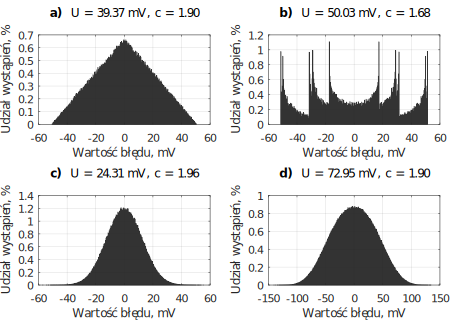
\includegraphics{obrazki/hist_part_S}
\DIFdelbeginFL %DIFDELCMD < \makecaption{fig:symul_partd_hist_S_2_0}{Histogramy realizacji sygnału błędu \textbf{a)}~statycznego, \textbf{b)}~dynamicznego, \textbf{c)}~losowego, \textbf{d)}~wypadkowego, wielkości wyjściowej $S_{2,0}$ analizowanego w eksperymencie symulacyjnym toru pomiarowego uzyskane metodą Monte-Carlo}
%DIFDELCMD < %%%
\DIFdelendFL \DIFaddbeginFL \makecaption{fig:symul_partd_hist_S_2_0}{Histogramy realizacji sygnału błędu \textbf{a)}~statycznego, \textbf{b)}~dynamicznego, \textbf{c)}~losowego, \textbf{d)}~wypadkowego wielkości wyjściowej $S_{2,0}$ analizowanego w eksperymencie symulacyjnym toru pomiarowego uzyskane metodą Monte-Carlo}
\DIFaddendFL \end{center}
\end{figure}

Na podstawie histogramów przedstawionych na rysunkach~\ref{fig:symul_partd_hist_S_2_0} oraz~\ref{fig:symul_partc_hist_T_1_0} zauważyć można, że oszacowane w równaniach od~\eqref{eq:sym_partd_output_unc_roun_S_2_0} do~\eqref{eq:sym_partd_output_unc_dyn_3_S_2_0} oraz od~\eqref{eq:sym_partd_output_unc_roun_T_1_0} do~\eqref{eq:sym_partd_output_unc_dyn_3_T_1_0} parametry sygnałów błędów pokrywają się z tymi uzyskanymi symulacyjnie. Współczynnik $A_{T_{1,0},s} $ określony w równaniu~\eqref{eq:sym_partd_output_as_T_1_0} wskazujący relacje pomiędzy wejściową i wyjściową wariancją błędów statycznych w przypadku wielkości wyjściowej $T_{1,0}$ jest w przybliżeniu równy zero. W rzeczywistości natomiast, ze względu na niewymierność kolejnych współczynników wiersza macierzy transformacji powiązanych z analizowaną wielkością wyjściową, współczynnik ten jest niezerowy. Fakt ten zauważyć można na podstawie rysunku~\ref{fig:symul_partc_hist_T_1_0}, gdzie teoretycznie wszystkie realizacje błędu statycznego powinny być zerowe. Omawiana rozbieżność jest jednak bardzo niewielka i nie wpływa zupełnie na uzyskane wyniki obliczeń.

\begin{figure}[htb!]
\begin{center}
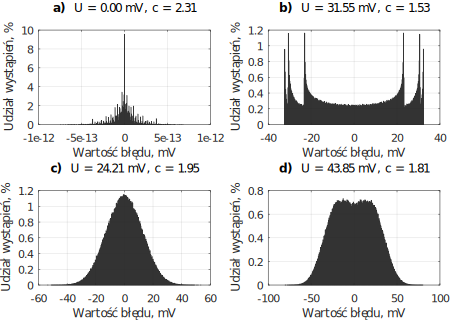
\includegraphics{obrazki/hist_part_T}
\DIFdelbeginFL %DIFDELCMD < \makecaption{fig:symul_partc_hist_T_1_0}{Histogramy realizacji sygnału błędu \textbf{a)}~statycznego, \textbf{b)}~dynamicznego, \textbf{c)}~losowego, \textbf{d)}~wypadkowego, wielkości wyjściowej $T_{1,0}$ analizowanego w eksperymencie symulacyjnym toru pomiarowego uzyskane metodą Monte-Carlo}
%DIFDELCMD < %%%
\DIFdelendFL \DIFaddbeginFL \makecaption{fig:symul_partc_hist_T_1_0}{Histogramy realizacji sygnału błędu \textbf{a)}~statycznego, \textbf{b)}~dynamicznego, \textbf{c)}~losowego, \textbf{d)}~wypadkowego wielkości wyjściowej $T_{1,0}$ analizowanego w eksperymencie symulacyjnym toru pomiarowego uzyskane metodą Monte-Carlo}
\DIFaddendFL \end{center}
\end{figure}

Ostatecznie wnioskować można, że przeprowadzony eksperyment \DIFdelbegin \DIFdel{wykazał }\DIFdelend \DIFaddbegin \DIFadd{potwierdził }\DIFaddend poprawność zaproponowanej metody analizy oraz stworzonego na potrzeby pracy modelu błędów. Oszacowana \DIFdelbegin \DIFdel{przy użyciu proponowanej metody }\DIFdelend wartość wariancji dla analizowanych sygnałów \DIFaddbegin \DIFadd{błędów była }\DIFaddend każdorazowo \DIFdelbegin \DIFdel{okazywała się }\DIFdelend zbieżna z wartością uzyskaną metodą symulacyjną. Uzyskane wartości niepewności \DIFdelbegin \DIFdel{rozszerzonej}\DIFdelend \DIFaddbegin \DIFadd{rozszerzonych}\DIFaddend , wyznaczane z użyciem redukcyjnej arytmetyki interwałowej, cechowały się rozbieżnością na poziomie mniejszym\DIFaddbegin \DIFadd{, }\DIFaddend niż wymagany w założeniach pracy. Eksperyment wykazał możliwość stosowania uproszczenia obliczeń, które wynika bezpośrednio z warunków centralnego twierdzenia granicznego\DIFdelbegin \DIFdel{, natomiast stosowanie go }\DIFdelend \DIFaddbegin \DIFadd{. Stosowanie omawianego uproszczenia }\DIFaddend dopuszczalne jest tylko i wyłącznie w określonych warunkach, natomiast w nieuzasadnionych przypadkach skutkować \DIFdelbegin \DIFdel{ono }\DIFdelend będzie przekraczającym~\qty{\pm 5}{\percent} błędem oszacowania \DIFaddbegin \DIFadd{wartości }\DIFaddend niepewności rozszerzonej.

Identyczną analizę wykonano wykorzystując budżet niepewności zestawiony w tabeli~\ref{tab:sym_partc_params_unc_list}. Parametry kolejnych składowych sygnałów błędów wyznaczono analogicznie, jak miało to miejsce w przykładach opisanych zależnościami od~\eqref{eq:sym_partd_output_var_stat_S_2_0} do~\eqref{eq:sym_partd_output_var_dyn_3_S_2_0} oraz od~\eqref{eq:sym_partd_output_unc_stat_S_2_0} do~\eqref{eq:sym_partd_output_unc_dyn_3_S_2_0}. W tabelach~\ref{tab:sym_partd_params_unc_list_S_2_0} oraz~\ref{tab:sym_partd_params_unc_list_T_1_0} zestawiono budżety niepewności dla analizowanych wielkości wyjściowych $S_{2,0}$ oraz $T_{1,0}$.

\DIFdelbegin %DIFDELCMD < \begin{table}[htb!]
%DIFDELCMD < \begin{center}
%DIFDELCMD < \makecaption{tab:sym_partd_params_unc_list_S_2_0}{Budżet niepewności wielkości wyjściowej $S_{2,0}$ analizowanego w eksperymencie symulacyjnym toru pomiarowego obejmujący wszystkie źródła błędów}
%DIFDELCMD < \begin{tabular}[c]{| c | c | S[table-format = 2.2] | S[table-format = 3.2] | c | c |} \hline
%DIFDELCMD < \textbf{Lp.} & \textbf{Symbol} & \textbf{$U$, mV} & \textbf{$\sigma^{2}$, \micro V} & \textbf{Rozkład} & \textbf{Źródło błędu} \\ \hline
%DIFDELCMD < 1  & ${rw,z}$     & 2.13  &   0.97  & zaokrągleń                   & operacje zmiennoprzecinkowe                \\ \hline
%DIFDELCMD < 2  & ${rp,q}$     & 13.26 &  45.78  & normalny                     & proces kwantowania (c)                     \\ \hline
%DIFDELCMD < 3  & ${rp,1}$     & 11.80 &  36.26  & normalny                     & nieliniowość obiektu (a)                   \\ \hline
%DIFDELCMD < 4  & ${rp,2}$     & 16.70 &  72.64  & normalny                     & szum wielkości wejściowej                  \\ \hline
%DIFDELCMD < 5  & ${sp,1}$     & 23.04 &  147.00 & trójkątny                    & dryft temperatury (a)                       \\ \hline
%DIFDELCMD < 6  & ${sp,2}$     & 16.29 &  73.52  & trójkątny                    & dryft temperatury (b)                       \\ \hline
%DIFDELCMD < 7  & ${dp,a,1}$   & 12.32 &  76.40  & \multirow{6}{*}{dwumodalny}  & \multirow{3}{*}{transmitancja (a)}         \\ \cline{1-4}
%DIFDELCMD < 8  & ${dp,a,2}$   & 25.08 &  316.38 &                              &                                            \\ \cline{1-4}
%DIFDELCMD < 9  & ${dp,a,3}$   & 2.35  &  2.77   &                              &                                            \\ \cline{1-4} \cline{6-6}
%DIFDELCMD < 10 & ${dp,b,1}$   & 6.07  &  18.52  &                              & \multirow{3}{*}{transmitancja (b)}         \\ \cline{1-4}
%DIFDELCMD < 11 & ${dp,b,2}$   & 12.35 &  76.70  &                              &                                            \\ \cline{1-4}
%DIFDELCMD < 12 & ${dp,b,3}$   & 1.16  &  0.67   &                              &                                            \\ \hline
%DIFDELCMD < \end{tabular}
%DIFDELCMD < \end{center}
%DIFDELCMD < \end{table}
%DIFDELCMD < %%%
\DIFdelend \DIFaddbegin \begin{table}[htb!]
\begin{center}
\makecaption{tab:sym_partd_params_unc_list_S_2_0}{Budżet niepewności wielkości wyjściowej $S_{2,0}$ analizowanego w eksperymencie symulacyjnym toru pomiarowego obejmujący wszystkie źródła błędów}
\begin{tabular}[c]{| c | c | S[table-format = 2.2] | S[table-format = 3.2] | c | c |} \hline
\textbf{Lp.} & \textbf{Symbol} & \textbf{$U$, mV} & \textbf{$\sigma^{2}$, \micro V} & \textbf{Rozkład} & \textbf{Źródło błędu} \\ \hline
1  & ${rw,z}$     & 2.13  &   0.97  & zaokrągleń                   & operacje zmiennoprzecinkowe                \\ \hline
2  & ${rp,q}$     & 13.26 &  45.78  & normalny                     & proces kwantowania ($c$)                   \\ \hline
3  & ${rp,1}$     & 11.80 &  36.26  & normalny                     & nieliniowość obiektu ($a$)                 \\ \hline
4  & ${rp,2}$     & 16.70 &  72.64  & normalny                     & szum wielkości wejściowej                  \\ \hline
5  & ${sp,1}$     & 23.04 &  147.00 & trójkątny                    & dryft temperatury ($a$)                    \\ \hline
6  & ${sp,2}$     & 16.29 &  73.52  & trójkątny                    & dryft temperatury ($b$)                    \\ \hline
7  & ${dp,a,1}$   & 12.32 &  76.40  & \multirow{6}{*}{dwumodalny}  & \multirow{3}{*}{transmitancja ($a$)}       \\ \cline{1-4}
8  & ${dp,a,2}$   & 25.08 &  316.38 &                              &                                            \\ \cline{1-4}
9  & ${dp,a,3}$   & 2.35  &  2.77   &                              &                                            \\ \cline{1-4} \cline{6-6}
10 & ${dp,b,1}$   & 6.07  &  18.52  &                              & \multirow{3}{*}{transmitancja ($b$)}       \\ \cline{1-4}
11 & ${dp,b,2}$   & 12.35 &  76.70  &                              &                                            \\ \cline{1-4}
12 & ${dp,b,3}$   & 1.16  &  0.67   &                              &                                            \\ \hline
\end{tabular}
\end{center}
\end{table}
\DIFaddend 

\DIFdelbegin %DIFDELCMD < \begin{table}[htb!]
%DIFDELCMD < \begin{center}
%DIFDELCMD < \makecaption{tab:sym_partd_params_unc_list_T_1_0}{Budżet niepewności wielkości wyjściowej $T_{1,0}$ analizowanego w eksperymencie symulacyjnym toru pomiarowego obejmujący wszystkie źródła błędów}
%DIFDELCMD < \begin{tabular}[c]{| c | c | S[table-format = 2.2] | S[table-format = 3.2] | c | c |} \hline
%DIFDELCMD < \textbf{Lp.} & \textbf{Symbol} & \textbf{$U$, mV} & \textbf{$\sigma^{2}$, \micro V} & \textbf{Rozkład} & \textbf{Źródło błędu} \\ \hline
%DIFDELCMD < 1  & ${rw,z}$     & 1.81  &  0.70   & zaokrągleń                   & operacje zmiennoprzecinkowe                \\ \hline
%DIFDELCMD < 2  & ${rp,q}$     & 13.26 &  45.78  & normalny                     & proces kwantowania (c)                     \\ \hline
%DIFDELCMD < 3  & ${rp,1}$     & 11.80 &  36.26  & normalny                     & nieliniowość obiektu (a)                   \\ \hline
%DIFDELCMD < 4  & ${rp,2}$     & 16.71 &  72.64  & normalny                     & szum wielkości wejściowej                  \\ \hline
%DIFDELCMD < 5  & ${sp,1}$     & 0.00  &  0.00   & trójkątny                    & dryft temperatury (a)                       \\ \hline
%DIFDELCMD < 6  & ${sp,2}$     & 0.00  &  0.00   & trójkątny                    & dryft temperatury (b)                       \\ \hline
%DIFDELCMD < 7  & ${dp,a,1}$   & 0.06  &  0.00   & \multirow{6}{*}{dwumodalny}  & \multirow{3}{*}{transmitancja (a)}         \\ \cline{1-4}
%DIFDELCMD < 8  & ${dp,a,2}$   & 3.77  &  7.13   &                              &                                            \\ \cline{1-4}
%DIFDELCMD < 9  & ${dp,a,3}$   & 19.16 &  184.65 &                              &                                            \\ \cline{1-4} \cline{6-6}
%DIFDELCMD < 10 & ${dp,b,1}$   & 0.03  &  0.00   &                              & \multirow{3}{*}{transmitancja (b)}         \\ \cline{1-4}
%DIFDELCMD < 11 & ${dp,b,2}$   & 1.85  &  1.73   &                              &                                            \\ \cline{1-4}
%DIFDELCMD < 12 & ${dp,b,3}$   & 9.44  &  44.82  &                              &                                            \\ \hline
%DIFDELCMD < \end{tabular}
%DIFDELCMD < \end{center}
%DIFDELCMD < \end{table}
%DIFDELCMD < %%%
\DIFdelend \DIFaddbegin \begin{table}[htb!]
\begin{center}
\makecaption{tab:sym_partd_params_unc_list_T_1_0}{Budżet niepewności wielkości wyjściowej $T_{1,0}$ analizowanego w eksperymencie symulacyjnym toru pomiarowego obejmujący wszystkie źródła błędów}
\begin{tabular}[c]{| c | c | S[table-format = 2.2] | S[table-format = 3.2] | c | c |} \hline
\textbf{Lp.} & \textbf{Symbol} & \textbf{$U$, mV} & \textbf{$\sigma^{2}$, \micro V} & \textbf{Rozkład} & \textbf{Źródło błędu} \\ \hline
1  & ${rw,z}$     & 1.81  &  0.70   & zaokrągleń                   & operacje zmiennoprzecinkowe                \\ \hline
2  & ${rp,q}$     & 13.26 &  45.78  & normalny                     & proces kwantowania ($c$)                   \\ \hline
3  & ${rp,1}$     & 11.80 &  36.26  & normalny                     & nieliniowość obiektu ($a$)                 \\ \hline
4  & ${rp,2}$     & 16.71 &  72.64  & normalny                     & szum wielkości wejściowej                  \\ \hline
5  & ${sp,1}$     & 0.00  &  0.00   & trójkątny                    & dryft temperatury ($a$)                    \\ \hline
6  & ${sp,2}$     & 0.00  &  0.00   & trójkątny                    & dryft temperatury ($b$)                    \\ \hline
7  & ${dp,a,1}$   & 0.06  &  0.00   & \multirow{6}{*}{dwumodalny}  & \multirow{3}{*}{transmitancja ($a$)}       \\ \cline{1-4}
8  & ${dp,a,2}$   & 3.77  &  7.13   &                              &                                            \\ \cline{1-4}
9  & ${dp,a,3}$   & 19.16 &  184.65 &                              &                                            \\ \cline{1-4} \cline{6-6}
10 & ${dp,b,1}$   & 0.03  &  0.00   &                              & \multirow{3}{*}{transmitancja ($b$)}       \\ \cline{1-4}
11 & ${dp,b,2}$   & 1.85  &  1.73   &                              &                                            \\ \cline{1-4}
12 & ${dp,b,3}$   & 9.44  &  44.82  &                              &                                            \\ \hline
\end{tabular}
\end{center}
\end{table}
\DIFaddend 

Ze względu na korelacje wybranych sygnałów błędów wielkości wejściowych rozważanego algorytmu, wyznaczenie wypadkowych wartości wariancji sygnałów błędów dla kolejnych wielkości wyjściowych przeprowadzane jest zgodnie z zależnością~\eqref{eq:var_matrix}. W dalszej części rozważań przyjęto, że symbol $\bsigma_{*}$ oznacza wektor złożony z odchyleń standardowych sygnałów błędów składowych wielkości wyjściowej algorytmu, przy czym \enquote{$*$} oznacza symbol analizowanej wielkości wyjściowej. Macierz korelacji oznaczona symbolem $\mathbf{r}_{d}$ jest jednakowa dla wszystkich wielkości wyjściowych tego algorytmu i składa się z dwunastu wierszy i kolumn, co wynika z liczby analizowanych sygnałów błędów. Przyjmuje się, że kolejne wielkości zawarte w wektorze $\bsigma_{*}$ oraz kolejne elementy macierzy $\mathbf{r}_{d}$ są związane z sygnałami błędów zestawionymi w tabelach~\ref{tab:sym_partd_params_unc_list_S_2_0} oraz~\ref{tab:sym_partd_params_unc_list_T_1_0}, a dodatkowo kolejność wyrazów omawianych wielkości jest zgodna z tą daną w tabelach. Wobec powyższych, równanie~\eqref{eq:var_matrix} przyjmuje postać:
\begin{equation}
\sigma_{*,\Sigma}^{2} = \bsigma_{*}^{T} \cdot \mathbf{r}_{d} \cdot \bsigma_{*} \label{eq:sym_partd_output_varmat_list}.
\end{equation}

Uwzględniając pełną dodatnią korelacje pary sygnałów błędów statycznych wzmacniacza i przetwornika pomiarowego przyjmuje się, że $r_{d,sp,1,2} = 1$. Dodatkowo na podstawie danych zawartych w tabelach~\ref{tab:sym_partb_params_dyn_self} oraz~\ref{tab:sym_partb_params_dyn_prop}, współczynniki korelacji kolejnych harmonicznych sygnału błędu dynamicznego o jednakowej częstotliwości są zbliżone do jedności, co wynika z równania~\eqref{eq:dyn_corr}, a zatem $r_{d,dp,a,b,n} = 1$ dla $n \in \{ 1, 2, 3 \}$. Wobec powyższych, kolejne elementy macierzy korelacji $\mathbf{r}_{d}$ przyjmują wartości:
\begin{equation}
\mathbf{r}_{d} =
\begin{bmatrix}
\num{1.0} & \num{0.0} & \num{0.0} & \num{0.0} & \num{0.0} & \num{0.0} & \num{0.0} & \num{0.0} & \num{0.0} & \num{0.0} & \num{0.0} & \num{0.0} \\
\num{0.0} & \num{1.0} & \num{0.0} & \num{0.0} & \num{0.0} & \num{0.0} & \num{0.0} & \num{0.0} & \num{0.0} & \num{0.0} & \num{0.0} & \num{0.0} \\
\num{0.0} & \num{0.0} & \num{1.0} & \num{0.0} & \num{0.0} & \num{0.0} & \num{0.0} & \num{0.0} & \num{0.0} & \num{0.0} & \num{0.0} & \num{0.0} \\
\num{0.0} & \num{0.0} & \num{0.0} & \num{1.0} & \num{0.0} & \num{0.0} & \num{0.0} & \num{0.0} & \num{0.0} & \num{0.0} & \num{0.0} & \num{0.0} \\
\num{0.0} & \num{0.0} & \num{0.0} & \num{0.0} & \num{1.0} & \num{1.0} & \num{0.0} & \num{0.0} & \num{0.0} & \num{0.0} & \num{0.0} & \num{0.0} \\
\num{0.0} & \num{0.0} & \num{0.0} & \num{0.0} & \num{1.0} & \num{1.0} & \num{0.0} & \num{0.0} & \num{0.0} & \num{0.0} & \num{0.0} & \num{0.0} \\
\num{0.0} & \num{0.0} & \num{0.0} & \num{0.0} & \num{0.0} & \num{0.0} & \num{1.0} & \num{0.0} & \num{0.0} & \num{1.0} & \num{0.0} & \num{0.0} \\
\num{0.0} & \num{0.0} & \num{0.0} & \num{0.0} & \num{0.0} & \num{0.0} & \num{0.0} & \num{1.0} & \num{0.0} & \num{0.0} & \num{1.0} & \num{0.0} \\
\num{0.0} & \num{0.0} & \num{0.0} & \num{0.0} & \num{0.0} & \num{0.0} & \num{0.0} & \num{0.0} & \num{1.0} & \num{0.0} & \num{0.0} & \num{1.0} \\
\num{0.0} & \num{0.0} & \num{0.0} & \num{0.0} & \num{0.0} & \num{0.0} & \num{1.0} & \num{0.0} & \num{0.0} & \num{1.0} & \num{0.0} & \num{0.0} \\
\num{0.0} & \num{0.0} & \num{0.0} & \num{0.0} & \num{0.0} & \num{0.0} & \num{0.0} & \num{1.0} & \num{0.0} & \num{0.0} & \num{1.0} & \num{0.0} \\
\num{0.0} & \num{0.0} & \num{0.0} & \num{0.0} & \num{0.0} & \num{0.0} & \num{0.0} & \num{0.0} & \num{1.0} & \num{0.0} & \num{0.0} & \num{1.0}
\end{bmatrix}
\label{eq:sym_partd_output_coher_list}.
\end{equation}

Zgodnie z zależnościami~\eqref{eq:sym_partd_output_varmat_list} oraz~\eqref{eq:sym_partd_output_coher_list}, po podstawieniu danych z tabel~\ref{tab:sym_partd_params_unc_list_S_2_0} oraz~\ref{tab:sym_partd_params_unc_list_T_1_0}, otrzymuje się wartości wariancji wypadkowych sygnałów błędów wielkości wyjściowych $S_{2,0}$ oraz $T_{1,0}$, przy czym kolejno:
\begin{gather}
\sigma_{S_{2,0},\Sigma}^{2} = \bsigma_{S_{2,0}}^{T} \cdot \mathbf{r}_{d} \cdot \bsigma_{S_{2,0}} = \qty{1464.79}{\micro V} \label{eq:sym_partd_output_varmat_S_2_0}, \\
\sigma_{T_{1,0},\Sigma}^{2} = \bsigma_{T_{1,0}}^{T} \cdot \mathbf{r}_{d} \cdot \bsigma_{T_{1,0}} = \qty{582.68}{\micro V} \label{eq:sym_partd_output_varmat_T_1_0}.
\end{gather}
Można zauważyć, że wyznaczone w ten sposób wartości są identyczne, jak te wyznaczone wcześniej w równaniach~\eqref{eq:sym_partd_output_var_sum_S_2_0} oraz~\eqref{eq:sym_partd_output_var_sum_T_1_0}.

Występowanie korelacji pomiędzy analizowanymi sygnałami błędów powoduje, że bezpośrednie zastosowanie metody opisanej równaniem~\eqref{eq:unc_matrix} dla współczynników koherencji wyznaczanych zgodnie z równaniem~\eqref{eq:unc_coher} nie jest możliwe. Aby umożliwić zastosowanie omawianej metody, proponuje się wyprowadzenie zależności opisujących wypadkowe parametry niepewności rozszerzonej dla grup skorelowanych sygnałów.

Dla sygnałów błędów statycznych wzmacniacza i przetwornika pomiarowego zapisać można następującą zależność, która określa wypadkową wartość niepewności rozszerzonej analizowanej pary sygnałów:
\begin{equation}
U_{*,sp} = \sqrt{
\begin{bmatrix}
U_{*,sp,1} \\ U_{*,sp,2}
\end{bmatrix}^{T}
\begin{bmatrix}
1 & h_{d,sp,1,2} \\
h_{d,sp,2,1} & 1
\end{bmatrix}
\begin{bmatrix}
U_{*,sp,1} \\ U_{*,sp,2}
\end{bmatrix}}
\label{eq:sym_partd_output_static_corrunc},
\end{equation}
przy czym w przypadku pełnej dodatniej korelacji tych sygnałów, tj. dla $r_{d,sp,1,2} = 1$, zachodzi $h_{d,sp,1,2} = 1$. Podobną zależność opisać można dla kolejnych par skorelowanych sygnałów błędów dynamicznych \DIFdelbegin \DIFdel{:
}\DIFdelend \DIFaddbegin \DIFadd{o jednakowej pulsacji:
}\DIFaddend \begin{equation}
U_{*,dp,n} = \DIFdelbegin \DIFdel{\sqrt{
\begin{bmatrix}
U_{*,dp,a,n} \\ U_{*,dp,b,n}
\end{bmatrix}^{T}
\begin{bmatrix}
1 & h_{d,dp,a,b,n} \\
h_{d,dp,x,2,1} & 1
\end{bmatrix}
\begin{bmatrix}
U_{*,dp,a,n} \\ U_{*,dp,b,n}
\end{bmatrix}}
}\DIFdelend \DIFaddbegin \DIFadd{\sqrt{
\begin{bmatrix}
U_{*,dp,a,n} \\ U_{*,dp,b,n}
\end{bmatrix}^{T}
\begin{bmatrix}
1 & h_{d,dp,a,b,n} \\
h_{d,dp,b,a,n} & 1
\end{bmatrix}
\begin{bmatrix}
U_{*,dp,a,n} \\ U_{*,dp,b,n}
\end{bmatrix}}
}\DIFaddend \label{eq:sym_partd_output_dynamic_corrunc},
\end{equation}
gdzie ze względu na pełną dodatnią korelację zachodzi \DIFdelbegin \DIFdel{$h_{d,dp,x,1,2} = 1$}\DIFdelend \DIFaddbegin \DIFadd{$h_{d,dp,a,b,n} = 1$}\DIFaddend . W analizowanych przypadkach, opisanych równaniami~\eqref{eq:sym_partd_output_static_corrunc} oraz~\eqref{eq:sym_partd_output_dynamic_corrunc}, zauważyć można, że wypadkowe sygnały błędów cechować się będą identycznymi kształtami \DIFdelbegin \DIFdel{rozkładu}\DIFdelend \DIFaddbegin \DIFadd{rozkładów}\DIFaddend , jak ich składowe.

Wobec powyższych, wektor niepewności rozszerzonych kolejnych sygnałów błędów dla wielkości wyjściowych analizowanego toru pomiarowego przedstawić można jako:
\begin{equation}
\mathbf{U}_{*} =
\begin{bmatrix}
U_{*,rw,z} & U_{*,rp,q} & U_{*,rp,1} & U_{*,rp,2} & U_{*,sp} & U_{*,dp,1} & U_{*,dp,2} & U_{*,dp,3}
\end{bmatrix}
\label{eq:sym_partd_output_unc_sumuvect},
\end{equation}
natomiast macierz koherencji, której wartości wyznaczane są zgodnie z równaniem~\eqref{eq:unc_coher}, opisać można dla kolejnych wielkości wyjściowych w postaci:
\begin{equation}
\mathbf{h}_{*} =
\begin{bmatrix}
1 & h_{*,0,1} & h_{*,0,2} & h_{*,0,3} & h_{*,0,4} & h_{*,0,5} & h_{*,0,6} & h_{*,0,7} \\
h_{*,1,0} & 1 & h_{*,1,2} & h_{*,1,3} & h_{*,1,4} & h_{*,1,5} & h_{*,1,6} & h_{*,1,7} \\
h_{*,2,0} & h_{*,2,1} & 1 & h_{*,2,3} & h_{*,2,4} & h_{*,2,5} & h_{*,2,6} & h_{*,2,7} \\
h_{*,3,0} & h_{*,3,1} & h_{*,3,2} & 1 & h_{*,3,4} & h_{*,3,5} & h_{*,3,6} & h_{*,3,7} \\
h_{*,4,0} & h_{*,4,1} & h_{*,4,2} & h_{*,4,3} & 1 & h_{*,4,5} & h_{*,4,6} & h_{*,4,7} \\
h_{*,5,0} & h_{*,5,1} & h_{*,5,2} & h_{*,5,3} & h_{*,5,4} & 1 & h_{*,5,6} & h_{*,5,7} \\
h_{*,6,0} & h_{*,6,1} & h_{*,6,2} & h_{*,6,3} & h_{*,6,4} & h_{*,6,5} & 1 & h_{*,6,7} \\
h_{*,7,0} & h_{*,7,1} & h_{*,7,2} & h_{*,7,3} & h_{*,7,4} & h_{*,7,5} & h_{*,7,6} & 1
\end{bmatrix}
\label{eq:sym_partd_output_unc_cohermat},
\end{equation}
przy czym kolejność elementów przedstawionej macierzy odpowiada kolejności elementów w wektorze niepewności rozszerzonych \DIFdelbegin \DIFdel{, }\DIFdelend opisanym równaniem~\eqref{eq:sym_partd_output_unc_sumuvect}, gdzie przykładowo $h_{*,0,1} = h_{*,rw,z,rp,q}$. Ostatecznie, wartość wypadkowej niepewności rozszerzonej może być oszacowana zgodnie z równaniem~\eqref{eq:unc_matrix}:
\begin{equation}
U_{*} = \sqrt{\mathbf{U}_{*} \cdot \mathbf{h}_{*} \cdot \mathbf{U}_{*}^{T}} \label{eq:sym_partd_output_unc_totalmat}.
\end{equation}

Podstawiając do równania~\eqref{eq:sym_partd_output_static_corrunc} wartości z tabel~\ref{tab:sym_partd_params_unc_list_S_2_0} oraz~\ref{tab:sym_partd_params_unc_list_T_1_0} otrzymuje się wypadkowe wartości niepewności \DIFdelbegin \DIFdel{rozszerzonej }\DIFdelend \DIFaddbegin \DIFadd{rozszerzonych }\DIFaddend dla sygnałów wypadkowych skorelowanych błędów statycznych wielkości $S_{2,0}$ oraz $T_{1,0}$\DIFdelbegin \DIFdel{w postaci}\DIFdelend \DIFaddbegin \DIFadd{, które wynoszą odpowiednio}\DIFaddend :
\begin{gather}
\begin{split}
U_{S_{2,0},sp} = & \sqrt{
\begin{bmatrix}
U_{S_{2,0},sp,1} \\ U_{S_{2,0},sp,2}
\end{bmatrix}^{T}
\begin{bmatrix}
1 & h_{d,sp,1,2} \\
h_{d,sp,2,1} & 1
\end{bmatrix}
\begin{bmatrix}
U_{S_{2,0},sp,1} \\ U_{S_{2,0},sp,2}
\end{bmatrix}} = \\ & \sqrt{
\begin{bmatrix}
\num{23.04e-3} \\ \num{16.29e-3}
\end{bmatrix}^{T}
\begin{bmatrix}
1 & 1 \\
1 & 1
\end{bmatrix}
\begin{bmatrix}
\num{23.04e-3} \\ \num{16.29e-3}
\end{bmatrix}} = \qty{39.31}{mV}
\end{split}
\label{eq:sym_partd_output_static_corrunc_S_2_0}, \\
\begin{split}
U_{T_{1,0},sp} = & \sqrt{
\begin{bmatrix}
U_{T_{1,0},sp,1} \\ U_{T_{1,0},sp,2}
\end{bmatrix}^{T}
\begin{bmatrix}
1 & h_{d,sp,1,2} \\
h_{d,sp,2,1} & 1
\end{bmatrix}
\begin{bmatrix}
U_{T_{1,0},sp,1} \\ U_{T_{1,0},sp,2}
\end{bmatrix}} = \\ & \sqrt{
\begin{bmatrix}
\num{0.00} \\ \num{0.00}
\end{bmatrix}^{T}
\begin{bmatrix}
1 & 1 \\
1 & 1
\end{bmatrix}
\begin{bmatrix}
\num{0.00} \\ \num{0.00}
\end{bmatrix}} = \qty{0.00}{mV}
\end{split}
\label{eq:sym_partd_output_static_corrunc__T_1_0},
\end{gather}
natomiast w przypadku równania~\eqref{eq:sym_partd_output_dynamic_corrunc} dla pierwszej harmonicznej sygnałów błędów dynamicznych omawianych wielkości zachodzi:
\begin{gather}
\begin{split}
U_{S_{2,0},dp,1} = & \sqrt{
\begin{bmatrix}
U_{S_{2,0},dp,a,1} \\ U_{S_{2,0},dp,b,1}
\end{bmatrix}^{T}
\begin{bmatrix}
1 & h_{d,dp,a,b,1} \\
h_{d,dp,b,a,1} & 1
\end{bmatrix}
\begin{bmatrix}
U_{S_{2,0},dp,a,1} \\ U_{S_{2,0},dp,b,1}
\end{bmatrix}} = \\ & \sqrt{
\begin{bmatrix}
\num{12.32e-3} \\ \num{6.07e-3}
\end{bmatrix}^{T}
\begin{bmatrix}
1 & 1 \\
1 & 1
\end{bmatrix}
\begin{bmatrix}
\num{12.32e-3} \\ \num{6.07e-3}
\end{bmatrix}} = \qty{18.39}{mV}
\end{split}
\label{eq:sym_partd_output_dynamic_corrunc_S_2_0}, \\
\begin{split}
U_{T_{1,0},dp,1} = & \sqrt{
\begin{bmatrix}
U_{T_{1,0},dp,a,1} \\ U_{T_{1,0},dp,b,1}
\end{bmatrix}^{T}
\begin{bmatrix}
1 & h_{d,dp,a,b,1} \\
h_{d,dp,b,a,1} & 1
\end{bmatrix}
\begin{bmatrix}
U_{T_{1,0},dp,a,1} \\ U_{T_{1,0},dp,b,1}
\end{bmatrix}} = \\ & \sqrt{
\begin{bmatrix}
\num{0.06e-3} \\ \num{0.03e-3}
\end{bmatrix}^{T}
\begin{bmatrix}
1 & 1 \\
1 & 1
\end{bmatrix}
\begin{bmatrix}
\num{0.06e-3} \\ \num{0.03e-3}
\end{bmatrix}} = \qty{0.092}{mV}
\end{split}
\label{eq:sym_partd_output_dynamic_corrunc_T_1_0}.
\end{gather}
Parametry pozostałych harmonicznych sygnałów błędów dynamicznych wyznaczono w analogiczny sposób, zatem obliczenia z nimi związane nie zostały przedstawione. Po podstawieniu uzyskanych wyników do równania~\eqref{eq:sym_partd_output_unc_sumuvect} otrzymuje się wektory składowych niepewności rozszerzonych dla analizowanych wielkości wyjściowych:
\begin{gather}
\mathbf{U}_{S_{2,0}} =
\begin{bmatrix}
\num{2.13} & \num{13.26} & \num{11.80} & \num{16.71} & \num{39.33} & \num{18.39} & \num{37.42} & \num{3.50}
\end{bmatrix} \cdot \num{e-3}
\label{eq:sym_partd_output_unc_sumuvect_S_2_0_b}, \\
\mathbf{U}_{T_{1,0}} =
\begin{bmatrix}
\num{1.81} & \num{13.26} & \num{11.80} & \num{16.71} & \num{0.00} & \num{0.092} & \num{5.62} & \num{28.60}
\end{bmatrix} \cdot \num{e-3}
\label{eq:sym_partd_output_unc_sumuvect_T_1_0_b},
\end{gather}
przy czym kolejne wyrazy macierzy koherencji dla analizowanych wielkości wyjściowych wyznaczane są zgodnie z równaniem~\eqref{eq:unc_coher}, a zatem przyjmują wartości:
\begin{gather}
\mathbf{h}_{S_{2,0}} =
\DIFdelbegin %DIFDELCMD < \begin{bmatrix}
%DIFDELCMD < 1 & h_{*,0,1} & h_{*,0,2} & h_{*,0,3} & h_{*,0,4} & h_{*,0,5} & h_{*,0,6} & h_{*,0,7} \\
%DIFDELCMD < h_{*,1,0} & 1 & h_{*,1,2} & h_{*,1,3} & h_{*,1,4} & h_{*,1,5} & h_{*,1,6} & h_{*,1,7} \\
%DIFDELCMD < h_{*,2,0} & h_{*,2,1} & 1 & h_{*,2,3} & h_{*,2,4} & h_{*,2,5} & h_{*,2,6} & h_{*,2,7} \\
%DIFDELCMD < h_{*,3,0} & h_{*,3,1} & h_{*,3,2} & 1 & h_{*,3,4} & h_{*,3,5} & h_{*,3,6} & h_{*,3,7} \\
%DIFDELCMD < h_{*,4,0} & h_{*,4,1} & h_{*,4,2} & h_{*,4,3} & 1 & h_{*,4,5} & h_{*,4,6} & h_{*,4,7} \\
%DIFDELCMD < h_{*,5,0} & h_{*,5,1} & h_{*,5,2} & h_{*,5,3} & h_{*,5,4} & 1 & h_{*,5,6} & h_{*,5,7} \\
%DIFDELCMD < h_{*,6,0} & h_{*,6,1} & h_{*,6,2} & h_{*,6,3} & h_{*,6,4} & h_{*,6,5} & 1 & h_{*,6,7} \\
%DIFDELCMD < h_{*,7,0} & h_{*,7,1} & h_{*,7,2} & h_{*,7,3} & h_{*,7,4} & h_{*,7,5} & h_{*,7,6} & 1
%DIFDELCMD < \end{bmatrix}%%%
\DIFdelend \DIFaddbegin \begin{bmatrix}
\num{1.000}  & \num{0.000} & \num{0.000} & \num{0.000} & \num{-0.001} & \num{0.006} & \num{0.017} & \num{0.001} \\
\num{0.000}  & \num{1.000} & \num{0.000} & \num{0.000} & \num{0.006}  & \num{0.033} & \num{0.072} & \num{0.007} \\
\num{0.000}  & \num{0.000} & \num{1.000} & \num{0.000} & \num{0.006}  & \num{0.029} & \num{0.066} & \num{0.006} \\
\num{0.000}  & \num{0.000} & \num{0.000} & \num{1.000} & \num{0.008}  & \num{0.045} & \num{0.086} & \num{0.010} \\
\num{-0.001} & \num{0.006} & \num{0.006} & \num{0.008} & \num{1.000}  & \num{0.116} & \num{0.259} & \num{0.042} \\
\num{0.006}  & \num{0.033} & \num{0.029} & \num{0.045} & \num{0.116}  & \num{1.000} & \num{0.223} & \num{0.028} \\
\num{0.017}  & \num{0.072} & \num{0.066} & \num{0.086} & \num{0.259}  & \num{0.223} & \num{1.000} & \num{0.079} \\
\num{0.001}  & \num{0.007} & \num{0.006} & \num{0.010} & \num{0.042}  & \num{0.028} & \num{0.079} & \num{1.000}
\end{bmatrix}\DIFaddend 
\label{eq:sym_partd_output_unc_cohermat_S_2_0_b}, \\
\mathbf{h}_{T_{1,0}} =
\DIFdelbegin %DIFDELCMD < \begin{bmatrix}
%DIFDELCMD < 1 & h_{*,0,1} & h_{*,0,2} & h_{*,0,3} & h_{*,0,4} & h_{*,0,5} & h_{*,0,6} & h_{*,0,7} \\
%DIFDELCMD < h_{*,1,0} & 1 & h_{*,1,2} & h_{*,1,3} & h_{*,1,4} & h_{*,1,5} & h_{*,1,6} & h_{*,1,7} \\
%DIFDELCMD < h_{*,2,0} & h_{*,2,1} & 1 & h_{*,2,3} & h_{*,2,4} & h_{*,2,5} & h_{*,2,6} & h_{*,2,7} \\
%DIFDELCMD < h_{*,3,0} & h_{*,3,1} & h_{*,3,2} & 1 & h_{*,3,4} & h_{*,3,5} & h_{*,3,6} & h_{*,3,7} \\
%DIFDELCMD < h_{*,4,0} & h_{*,4,1} & h_{*,4,2} & h_{*,4,3} & 1 & h_{*,4,5} & h_{*,4,6} & h_{*,4,7} \\
%DIFDELCMD < h_{*,5,0} & h_{*,5,1} & h_{*,5,2} & h_{*,5,3} & h_{*,5,4} & 1 & h_{*,5,6} & h_{*,5,7} \\
%DIFDELCMD < h_{*,6,0} & h_{*,6,1} & h_{*,6,2} & h_{*,6,3} & h_{*,6,4} & h_{*,6,5} & 1 & h_{*,6,7} \\
%DIFDELCMD < h_{*,7,0} & h_{*,7,1} & h_{*,7,2} & h_{*,7,3} & h_{*,7,4} & h_{*,7,5} & h_{*,7,6} & 1
%DIFDELCMD < \end{bmatrix}%%%
\DIFdelend \DIFaddbegin \begin{bmatrix}
\num{1.000} & \num{0.000} & \num{0.000} & \num{0.000} & \num{0.000} & \num{0.000} & \num{0.021} & \num{0.021} \\
\num{0.000} & \num{1.000} & \num{0.000} & \num{0.000} & \num{0.000} & \num{0.006} & \num{0.093} & \num{0.092} \\
\num{0.000} & \num{0.000} & \num{1.000} & \num{0.000} & \num{0.000} & \num{0.005} & \num{0.084} & \num{0.084} \\
\num{0.000} & \num{0.000} & \num{0.000} & \num{1.000} & \num{0.000} & \num{0.009} & \num{0.117} & \num{0.116} \\
\num{0.000} & \num{0.000} & \num{0.000} & \num{0.000} & \num{1.000} & \num{0.000} & \num{0.000} & \num{0.000} \\
\num{0.000} & \num{0.006} & \num{0.005} & \num{0.009} & \num{0.000} & \num{1.000} & \num{0.042} & \num{0.042} \\
\num{0.021} & \num{0.093} & \num{0.084} & \num{0.117} & \num{0.000} & \num{0.042} & \num{1.000} & \num{0.497} \\
\num{0.021} & \num{0.092} & \num{0.084} & \num{0.116} & \num{0.000} & \num{0.042} & \num{0.497} & \num{1.000}
\end{bmatrix}\DIFaddend 
\label{eq:sym_partd_output_unc_cohermat_T_1_0_b}.
\end{gather}
Po podstawieniu powyższych wartości do równania~\eqref{eq:sym_partd_output_unc_totalmat} otrzymuje się wartości wypadkowych niepewności rozszerzonych analizowanych wielkości wyjściowych toru pomiarowego, gdzie kolejno \DIFaddbegin \DIFadd{wynoszą one}\DIFaddend :
\begin{gather}
U_{S_{2,0}} = \sqrt{\mathbf{U}_{S_{2,0}} \cdot \mathbf{h}_{S_{2,0}} \cdot \mathbf{U}_{S_{2,0}}^{T}} = \qty{74.10}{mV} \label{eq:sym_partd_output_unc_totalmat_S_2_0}, \\
U_{T_{1,0}} = \sqrt{\mathbf{U}_{T_{1,0}} \cdot \mathbf{h}_{T_{1,0}} \cdot \mathbf{U}_{T_{1,0}}^{T}} = \qty{43.37}{mV} \label{eq:sym_partd_output_unc_totalmat_T_1_0}.
\end{gather}

Przedstawione w równaniach~\eqref{eq:sym_partd_output_unc_totalmat_S_2_0} oraz~\eqref{eq:sym_partd_output_unc_totalmat_T_1_0} obliczenia wykonano ponownie, dla macierzy koherencji których wartości wyznaczone zostały bez uwzględnienia korekty zaproponowanej w równaniu~\eqref{eq:unc_cohercorra}, tj. kiedy w równaniu~\eqref{eq:unc_coher} przyjmuje się $p_{i,j} = 1$ dla dowolnej pary $i$ oraz $j$. Otrzymane wartości wyniosły kolejno $U_{S_{2,0}} = \qty{77.32}{mV}$ oraz $U_{T_{1,0}} = \qty{46.09}{mV}$. Podobne obliczenia wykonano dla pozostałych wielkości wyjściowych.

W tabeli~\ref{tab:sym_partd_params_unc_sum_b} zestawiono wyniki obliczeń dla pozostałych wielkości wyjściowych oraz te uzyskane w poprzednim eksperymencie, w celu umożliwienia ich porównania. Symbolem \DIFdelbegin \DIFdel{$a$ }\DIFdelend \DIFaddbegin \DIFadd{$U_{a}$ }\DIFaddend oznaczono wartości uzyskane przy założeniu normalnego rozkładu sygnału błędu wypadkowego, \DIFdelbegin \DIFdel{symbolem $b$ }\DIFdelend \DIFaddbegin \DIFadd{natomiast symbolem $U_{b}$ }\DIFaddend oznaczono wartości uzyskane z wykorzystaniem budżetu niepewności opisanego w tabeli~\ref{tab:sym_partc_params_unc_sum}. Wartości oznaczone symbolem \DIFdelbegin \DIFdel{$c$ }\DIFdelend \DIFaddbegin \DIFadd{$U_{c}$ }\DIFaddend dotyczą analizy z wykorzystaniem budżetu niepewności opisanego w tabeli~\ref{tab:sym_partc_params_unc_list}, przy czym wielkości oznaczone symbolem \DIFdelbegin \DIFdel{$d$ }\DIFdelend \DIFaddbegin \DIFadd{$U_{d}$ }\DIFaddend wyznaczono identycznie, jak \DIFdelbegin \DIFdel{dla $c$}\DIFdelend \DIFaddbegin \DIFadd{$U_{c}$}\DIFaddend , z tą różnicą\DIFaddbegin \DIFadd{, }\DIFaddend że nie stosowano korekty opisanej równaniem~\eqref{eq:unc_cohercorra} w procesie wyznaczania wartości współczynników koherencji. Podobnie, jak w zestawieniu zawartym w tabeli~\ref{tab:sym_partd_params_unc_sum_a}, wielkości oznaczone symbolem \DIFdelbegin \DIFdel{$s$ }\DIFdelend \DIFaddbegin \DIFadd{$U_{s}$ }\DIFaddend dotyczą przeprowadzonego eksperymentu metodą Monte-Carlo, natomiast symbolem $\delta_{*}$ oznaczono \DIFaddbegin \DIFadd{wyrażony w procentach }\DIFaddend błąd względny oszacowania wartości niepewności rozszerzonej \DIFdelbegin \DIFdel{metodą $a$, $b$, $c$ oraz $d$ }\DIFdelend \DIFaddbegin \DIFadd{$U_{*}$ }\DIFaddend w odniesieniu do wartości $U_{s}$, \DIFdelbegin \DIFdel{wyrażony w procentach, }\DIFdelend wyznaczany zgodnie z zależnością~\eqref{eq:unc_error}.

\begin{table}[htb!]
\begin{center}
\makecaption{tab:sym_partd_params_unc_sum_b}{Porównanie uzyskanych przedstawionymi w pracy metodami wartości wypadkowych niepewności rozszerzonych kolejnych wielkości wyjściowych analizowanego w eksperymencie symulacyjnym toru pomiarowego}
\begin{tabular}[c]{| c *{5}{|S[table-format = 2.2]} *{4}{|S[table-format = +1.2]} |} \hline
\multirow{2}{*}{\textbf{Wielkość}} & \multicolumn{5}{c|}{\textbf{Niepewność, mV}} & \multicolumn{4}{c|}{\textbf{Błąd, \%}} \\ \cline{2-10}
& $U_{a}$ & $U_{b}$ & $U_{c}$ & $U_{d}$ & $U_{s}$ & $\delta_{a}$ & $\delta_{b}$ & $\delta_{c}$ & $\delta_{d}$ \\ \hline
$S_{2,0}$ & 75.01 & 74.00 & 74.10 & 77.32 & 72.87 & +2.94 & +1.55 & +1.69 & +6.11 \\ \hline
$S_{2,1}$ & 68.19 & 68.44 & 68.43 & 71.52 & 67.09 & +1.64 & +2.01 & +2.00 & +6.60 \\ \hline
$T_{2,0}$ & 57.29 & 56.26 & 55.91 & 57.58 & 53.89 & +6.31 & +4.40 & +3.75 & +6.85 \\ \hline
$T_{2,1}$ & 58.86 & 55.59 & 55.60 & 59.47 & 54.92 & +7.17 & +1.22 & +1.24 & +8.28 \\ \hline
$T_{1,0}$ & 47.31 & 43.61 & 43.37 & 46.09 & 43.76 & +8.11 & -0.34 & -0.89 & +5.32 \\ \hline
$T_{1,1}$ & 47.31 & 43.60 & 43.37 & 46.08 & 43.74 & +8.16 & -0.32 & -0.85 & +5.35 \\ \hline
$T_{1,2}$ & 47.31 & 43.60 & 43.37 & 46.08 & 43.76 & +8.11 & -0.37 & -0.89 & +5.30 \\ \hline
$T_{1,3}$ & 44.79 & 43.64 & 43.39 & 45.43 & 43.17 & +3.75 & +1.09 & +0.51 & +5.24 \\ \hline
\end{tabular}
\end{center}
\end{table}

Analizując wyniki przedstawione w tabeli~\ref{tab:sym_partd_params_unc_sum_b} zauważyć można, że zaproponowana w pracy metoda szacowania wypadkowej wartości niepewności rozszerzonej wraz z zastosowaniem proponowanego modelu błędów zapewniają wyniki zbieżne z tymi uzyskanymi symulacyjnie. Korekta wartości współczynników koherencji opisana równaniem~\eqref{eq:unc_cohercorra} pozwala na znaczne zmniejszenie rozbieżności pomiędzy szacowaną zgodnie z równaniem~\eqref{eq:unc_matrix} wartością, a wartością uzyskiwaną symulacyjnie, w stosunku do wartości uzyskanych bez stosowania opisanej korekty. Wartości uzyskane przy zastosowaniu budżetu niepewności zawierającego jedynie wypadkowe parametry sygnałów błędów z uwzględnieniem na wprowadzone kategorie błędów są zbieżne z wartościami uzyskanymi dla budżetu obejmującego charakterystykę każdego z sygnałów błędów. Rozbieżności pomiędzy wartościami oznaczonymi symbolami \DIFdelbegin \DIFdel{$b$ oraz $c$ }\DIFdelend \DIFaddbegin \DIFadd{$U_{b}$ oraz $U_{c}$ }\DIFaddend wynikają z innego oszacowania wartości współczynników koherencji.

\section{Podsumowanie rozdziału}

Przedstawione w bieżącym rozdziale rozważania i przeprowadzone eksperymenty potwierdzają poprawność proponowanego w pracy modelu błędów oraz skuteczność stosowanej metody redukcyjnej arytmetyki interwałowej. Oszacowane zgodnie z równaniem~\eqref{eq:unc_matrix} wartości wypadkowej niepewności rozszerzonej dla współczynników koherencji szacowanych zgodnie z zależnością~\eqref{eq:unc_coher} każdorazowo okazywały się zbieżne z wynikami uzyskiwanymi dla przeprowadzonych metodą Monte-Carlo eksperymentów. Wartości niepewności rozszerzonych oszacowane stosując zaproponowaną w pracy korektę wartości współczynników koherencji, daną równaniem~\eqref{eq:unc_cohercorra}, były bliższe uzyskanym eksperymentalnie. W praktyce pomiarowej zaproponowana korekta wartości współczynników koherencji nie jest wymagana, jeżeli dopuszcza się przekraczający~\qty{5}{\percent} względny błąd oszacowania wartości wypadkowej niepewności rozszerzonej. Należy również brać pod uwagę, że oszacowane w proponowany sposób wartości niepewności rozszerzonej mogą być w pewnych przypadkach nieco niższe, niż wartości prawdziwe. Różnice te nie przekraczają jednak~\qty{-3}{\percent} wartości prawdziwej, co wykazano w eksperymencie, którego wyniki przedstawiono wcześniej na rysunku~\ref{fig:hist_reductive} oraz w przedstawionych dotychczas przykładach obliczeń.

W przypadku, gdy analizowane sygnały błędów składowych cechować się będą nietypowym rozkładem \DIFaddbegin \DIFadd{realizacji tych sygnałów}\DIFaddend , stosowanie omawianej w pracy metody wymagać będzie wyznaczenia wartości współczynników kształtu dla wszystkich analizowanych typów rozkładów. Jest to jedyna czynność, której przeprowadzenie nie będzie mogło zwykle odbywać się w czasie pracy systemu pomiarowego i będzie musiała ona zostać przeprowadzona na etapie identyfikacji jego właściwości\DIFaddbegin \DIFadd{~\mbox{%DIFAUXCMD
\cite{auth_reductive}}\hskip0pt%DIFAUXCMD
}\DIFaddend . Podobny problem napotkać można w przypadku wystąpienia korelacji pomiędzy analizowanymi sygnałami błędów składowych -- należy wtedy postąpić identycznie, jak pokazano w przykładzie lub zastosować inną metodę wyznaczania wartości elementów macierzy koherencji, jak chociażby pokazano w pracy~\cite{jakubiec_reductive}.

Przedstawiona w równaniach od~\eqref{eq:sym_partd_output_static_corrunc} do~\eqref{eq:sym_partd_output_unc_totalmat} analiza umożliwiła wykorzystanie zaproponowanej metody szacowania wartości współczynników koherencji, opisanej równaniem~\eqref{eq:unc_coher} mimo, że metoda ta nie jest odpowiednia dla analizy skorelowanych sygnałów. Możliwość zastosowania opisanego algorytmu wynika z faktu, że wypadkowe sygnały dla skorelowanych grup sygnałów cechują się typowym kształtem rozkładu, dla którego wyznaczono wcześniej wartości współczynników kształtu. W innych okolicznościach należałoby wyznaczyć odpowiednie dla analizowanych parametrów sygnałów wartości współczynników koherencji.

Jako, że żaden z etapów szacowania wypadkowej wartości niepewności rozszerzonej zgodnie z zaproponowaną metodą nie wymaga przeprowadzania dodatkowych symulacji metodą Monte-Carlo, a wykonywane obliczenia sprowadzają się w większości przypadków do prostych operacji arytmetycznych, przedstawiona metoda może zostać zaimplementowana w torze pomiarowym w celu bieżącej oceny jego właściwości metrologicznych. W przypadku zmiany parametrów sygnałów błędów obecnych w analizowanym torze pomiarowym wymagane jest jedynie ponowne wyznaczenie wartości macierzy koherencji i wskazanie parametrów istniejących sygnałów błędów. Istotnymi parametrami analizowanych sygnałów błędów jest w tym przypadku wartość niepewności rozszerzonej dla wybranego, identycznego dla wszystkich wielkości poziomu ufności oraz rodzaj rozkładu \DIFaddbegin \DIFadd{realizacji }\DIFaddend analizowanego sygnału.

Stosowanie uproszczenia, gdzie zakłada się normalny rozkład \DIFaddbegin \DIFadd{realizacji sygnału }\DIFaddend błędu wypadkowego, pozwala znacznie uprościć proces wyznaczania wypadkowej wartości niepewności rozszerzonej i zastąpić konieczność stosowania zależności~\eqref{eq:unc_matrix} oraz~\eqref{eq:unc_coher} wyznaczeniem wariancji wypadkowego sygnału błędu\DIFdelbegin \DIFdel{, natomiast jego stosowanie }\DIFdelend \DIFaddbegin \DIFadd{. Stosowanie omawianego uproszczenia }\DIFaddend wymaga posiadania pewności odnoście spełnienia warunków centralnego twierdzenia granicznego. Jak wykazały przeprowadzone eksperymenty, nawet dla kilkunastu źródeł błędów, gdzie większość z nich nie jest wzajemnie skorelowana, założenie to może okazać się niespełnione, co skutkuje znaczną rozbieżnością pomiędzy oszacowaną, a prawdziwą wartością niepewności rozszerzonej na poziomie zbliżonym do~\DIFdelbegin %DIFDELCMD < \qty{10}{\percent}%%%
\DIFdelend \DIFaddbegin \qty{\pm 10}{\percent}\DIFaddend .

Mimo, że wprowadzenie do proponowanego modelu błędów funkcji przetwarzania obiektu może być zastąpione wprowadzeniem statycznego wzmocnienia w równaniu transmitancji obiektu, obecność tej funkcji umożliwia bardziej spójną \DIFdelbegin \DIFdel{w }\DIFdelend \DIFaddbegin \DIFadd{i }\DIFaddend logiczną analizę rzeczywistych obiektów. Nawet, jeśli rzeczywista postać funkcji przetwarzania nie jest znana, to wprowadzany przez nią sygnał błędu można opisać odpowiednią zależnością lub wskazać jego parametry, jak pokazano w omówionym przykładzie. Przeprowadzone badania wykazały, że w przypadku nieznanej rzeczywistej funkcji przetwarzania obiektu do oszacowania wpływu tej funkcji na postać sygnałów na wyjściu obiektu, wykorzystać można jej idealne równanie przetwarzania. Wskazana właściwość jest bardzo cenna w przypadku nieliniowości charakterystyki obiektu lub analizy przetwornika analogowo-cyfrowego.

\chapter{Pomiarowa weryfikacja tezy}

Ostatni etap \DIFdelbegin \DIFdel{weryfikacji postawionej w pracy tezy }\DIFdelend \DIFaddbegin \DIFadd{pracy }\DIFaddend stanowi analiza właściwości metrologicznych \DIFdelbegin \DIFdel{przykładowego }\DIFdelend \DIFaddbegin \DIFadd{zbudowanego na jej potrzeby }\DIFaddend toru pomiarowego, \DIFdelbegin \DIFdel{który stworzony został na potrzeby pracy}\DIFdelend \DIFaddbegin \DIFadd{którego schemat blokowy przedstawiono na rysunku~\ref{fig:chain_real}}\DIFaddend . Analizowany tor pomiarowy przetwarza zmienny w czasie sygnał napięciowy $s(t)$ o chwilowej wartości napięcia z przedziału \DIFdelbegin \DIFdel{$\hat{s}(t) \in~<0;1>~\unit{V}$}\DIFdelend \DIFaddbegin \DIFadd{$\hat{s}(t) \in \interval{1}{0}~\unit{V}$}\DIFaddend . W celu dopasowania \DIFdelbegin \DIFdel{poziomu sygnału }\DIFdelend \DIFaddbegin \DIFadd{wartości }\DIFaddend napięcia \DIFdelbegin \DIFdel{wejściowego }\DIFdelend \DIFaddbegin \DIFadd{sygnału $s(t)$ }\DIFaddend do zakresu napięcia wejściowego przetwornika analogowo-cyfrowego oraz zwiększenia impedancji wejściowej toru pomiarowego, sygnał $s(t)$ podawany jest na wejście wzmacniacza pomiarowego. Sygnał wyjściowy $y(t)$ wzmacniacza \DIFaddbegin \DIFadd{podawany jest następnie na wejście zintegrowanego z układem próbkująco-pamiętającym przetwornika analogowo-cyfrowego, gdzie }\DIFaddend przetwarzany jest na postać cyfrową\DIFdelbegin \DIFdel{$c(i)$, a następnie po }\DIFdelend \DIFaddbegin \DIFadd{, oznaczoną $c(i)$. Po }\DIFaddend wykonaniu odtwarzania statycznego, \DIFaddbegin \DIFadd{sygnał $s(t)$ }\DIFaddend podawany jest w postaci wielkości $x(i)$ na wejście jednostki \enquote{DSP}\DIFdelbegin \DIFdel{, która dla }\DIFdelend \DIFaddbegin \DIFadd{. Dla }\DIFaddend każdego $j$-tego okna pomiarowego \DIFdelbegin \DIFdel{pobiera }\DIFdelend \DIFaddbegin \DIFadd{pobieranych jest }\DIFaddend $N$ próbek \DIFdelbegin \DIFdel{tego }\DIFdelend sygnału \DIFdelbegin \DIFdel{i wyznacza na ich podstawie }\DIFdelend \DIFaddbegin \DIFadd{$x(i)$, a następnie wyznaczanych jest }\DIFaddend $M$ wartości wielkości wyjściowych wektora $\mathbf{X}(j)$, stosując w tym celu algorytm dyskretnej transformacji falkowej.
\DIFdelbegin \DIFdel{Schemat blokowy omawianego toru pomiarowego przedstawiono na rysunku~\ref{fig:chain_real}.
}\DIFdelend 

\begin{figure}[htb!]
\begin{center}
\includegraphics{obrazki/schemat_real}
\DIFdelbeginFL %DIFDELCMD < \makecaption{fig:chain_real}{Schemat blokowy stworzonego na potrzeby pracy toru pomiarowego będącego obiektem przeprowadzanego eksperymentu}
%DIFDELCMD < %%%
\DIFdelendFL \DIFaddbeginFL \makecaption{fig:chain_real}{Schemat blokowy stworzonego na potrzeby pracy toru pomiarowego, będącego obiektem przeprowadzanego eksperymentu}
\DIFaddendFL \end{center}
\end{figure}

Do realizacji układu wzmacniacza pomiarowego zastosowany został wzmacniacz operacyjny \enquote{MCP6002}~\cite{microchip_manual} w konfiguracji nieodwracającej, o docelowym wzmocnieniu wynoszącym~\qty{3.3}{V \per V}. Napięcie zasilania wzmacniacza wynosi~\qty{3.3}{V} i pochodzi ze stabilizatora \enquote{LD1117}~\cite{stm_manual} typu \enquote{LDO} (ang. \enquote{Low Dropout}). Zaproponowana konfiguracja zapewnia wysoką impedancję wejściową toru pomiarowego oraz bardzo niską impedancję wyjściową wzmacniacza. \DIFdelbegin \DIFdel{Parametry statyczne oraz dynamiczne analizowanego obiektu wymagają identyfikacji, ze względu na niedostateczne informacje zawarte w dokumentacji układu. Na }\DIFdelend \DIFaddbegin \DIFadd{Zgodnie z zaleceniami zawartymi w~\mbox{%DIFAUXCMD
\cite{baker_sar, microchip_application}}\hskip0pt%DIFAUXCMD
, na }\DIFaddend wyjściu wzmacniacza zastosowano dodatkowy filtr RC\DIFaddbegin \DIFadd{, }\DIFaddend złożony z rezystancji~\qty{100}{\ohm} oraz pojemności~\qty{48}{nF}\DIFdelbegin \DIFdel{, zgodnie z zaleceniami zawartymi w~\mbox{%DIFAUXCMD
\cite{baker_sar, microchip_application}}\hskip0pt%DIFAUXCMD
}\DIFdelend . Przyjmuje się, że oznaczony na rysunku~\ref{fig:chain_real} sygnał $y(t)$ jest sygnałem na wyjściu omawianego filtru. Nominalne wartości rezystorów w dzielniku napięcia pętli sprzężenia zwrotnego wynoszą kolejno~\qty{220}{k \ohm} oraz~\qty{100}{k \ohm}, natomiast zastosowane w celu realizacji prototypu układu rezystory zostały dobrane tak, aby osiągnąć wymagane wzmocnienie. \DIFaddbegin \DIFadd{Ze względu na niedostateczne informacje zawarte w dokumentacji układu~\mbox{%DIFAUXCMD
\cite{microchip_manual}}\hskip0pt%DIFAUXCMD
, parametry statyczne oraz dynamiczne analizowanego obiektu wymagają pomiarowej identyfikacji.
}\DIFaddend 

\DIFdelbegin \DIFdel{Zastosowany przetwornik analogowo-cyfrowy stanowi}\DIFdelend \DIFaddbegin \DIFadd{Przetwarzanie analogowo-cyfrowe realizowane jest przez}\DIFaddend ~\qty{12}{\bitOwy} przetwornik wagowy \enquote{SAR} (ang. \enquote{Successive Approximation Register}), który zintegrowany jest w mikrokontrolerze \enquote{STM32F411}~\cite{stm_f411}. Źródło napięcia odniesienia stanowi w jego przypadku stabilizator \enquote{AP7343}~\cite{diodes_manual} typu \enquote{LDO}, o znamionowym napięciu wyjściowym równym~\qty{3.3}{V}, przyłączony z użyciem dodatkowego filtru LC. Przetwornik analogowo-cyfrowy taktowany jest sygnałem zegarowym o częstotliwości~\qty{12}{MHz}, przy czym próbkowanie inicjowane jest sygnałem z licznika, którego częstotliwość wyzwalania wynosi $f_{s} = \qty{48}{kHz}$. Po wyzwoleniu sygnału z licznika następuje śledzenie napięcia wejściowego, trwające~\qty{144}{takty} zegara, po którym wykonywana jest konwersja analogowo-cyfrowa, trwająca~\qty{15}{taktów} zegara, co w analizowanym przypadku stanowi łączny czas~\qty{13.25}{\micro s}. Ze względu na typowe zastosowanie omawianego przetwornika, jego najistotniejsze parametry, konieczne do aplikacji zaproponowanego w pracy modelu błędów, mogą zostać pozyskane z dokumentacji producenta układu~\cite{stm_f411}. Dodatkowy algorytm odtwarzania statycznego przekształca sygnał wyjściowy $c(i)$ przetwornika analogowo-cyfrowego na sygnał $x(i)$ tak, aby stanowił on dyskretną reprezentację sygnału $s(t)$ o czułości~\qty{1}{V \per V} względem tego sygnału.

Pozyskane próbki \DIFdelbegin \DIFdel{napięcia }\DIFdelend \DIFaddbegin \DIFadd{wielkości }\DIFaddend $x(i)$, stanowiące dyskretną reprezentację sygnału wejściowego $s(t)$, zapisywane są w wektorze $\mathbf{x}(j)$ o długości $N = 128$. Wektor wielkości wejściowych $\mathbf{x}(j)$ podawany jest na wejście algorytmu dyskretnej transformacji falkowej, którego implementacja zrealizowana została z wykorzystaniem instrukcji \enquote{DSP} dostępnych dla zastosowanego mikrokontrolera~\cite{cortex_dsp, reay_dsp}. Analizowany algorytm wykorzystuje falkę \enquote{spline4:4}~\cite{wang_splinebasics} dla pięciu iteracji procesu dekompozycji sygnału. Zgodnie z równaniem~\eqref{eq:alg_out_mat} wyznaczanych jest $M = 128$ próbek wektora wielkości wyjściowych $\mathbf{X}(j)$, które stanowią wyjście dla pojedynczej $j$-tej serii pomiarowej analizowanego toru pomiarowego. Wartości elementów macierzy transformacji $\mathbf{A}$ zidentyfikowano zgodnie z metodą przedstawioną w równaniu~\eqref{eq:wt_ident}, wykorzystując w tym celu implementację algorytmu transformacji falkowej dostępną w programie \enquote{GNU Octave}~\cite{pruuvsa_dwt}. Czas obliczeń wynosi w analizowanym przypadku \DIFdelbegin \DIFdel{~}%DIFDELCMD < \qty{1508}{\micro s}%%%
\DIFdelend \DIFaddbegin \DIFadd{około~}\qty{1.5}{ms}\DIFaddend , przy czym łączny czas akwizycji pojedynczego wektora próbek wielkości wejściowych wynosi~\DIFdelbegin %DIFDELCMD < \qty{2666.67}{\micro s}%%%
\DIFdelend \DIFaddbegin \qty{2.67}{ms}\DIFaddend . Podczas obliczeń stosowane są liczby zmiennoprzecinkowe pojedynczej precyzji o długości słowa~\qty{32}{\bitOw}, implementowane sprzętowo przez jednostkę \enquote{FPU}\DIFdelbegin \DIFdel{(ang. }%DIFDELCMD < \enquote{Floating Point Unit}%%%
\DIFdel{)}\DIFdelend \DIFaddbegin \DIFadd{, obecną w zastosowanym mikrokontrolerze}\DIFaddend ~\cite{cortex_fpu, gcc_manual}.

Przedstawiony tor pomiarowy pracuje w trybie ciągłym, tj. w pojedynczym $j$-tym oknie pomiarowym, w czasie pobierania wartości realizacji kolejnych wielkości wejściowych wektora $\mathbf{x}(j)$, wyznaczana jest realizacja wektora wielkości wyjściowych $\mathbf{X}(j-1)$ dla poprzedniej realizacji wektora wielkości wejściowych $\mathbf{x}(j-1)$. Wykorzystywany jest w tym celu kontroler \enquote{DMA}, nadzorujący proces buforowania kolejnych realizacji sygnału \DIFdelbegin \DIFdel{$x(i)$}\DIFdelend \DIFaddbegin \DIFadd{$s(t)$}\DIFaddend , w czasie gdy program główny wykonuje obliczenia dane równaniem~\eqref{eq:alg_out_mat}. Analiza wartości wielkości wyjściowych omawianego toru pomiarowego jest możliwa między innymi po podłączeniu go do komputera klasy \enquote{PC} za pośrednictwem portu \enquote{USB}, przy czym wykorzystywany jest w tym celu układ peryferyjny \enquote{USB OTG Full-Speed}, zintegrowany w zastosowanym mikrokontrolerze. Alternatywną możliwość wymiany informacji z urządzeniem stanowi interfejs \enquote{UART}, natomiast ze względu na ograniczenie szybkości transferu danych przez ten interfejs, nie umożliwia on ciągłego śledzenia wyników pomiarów.

W dalszej części rozdziału opisano najważniejsze źródła błędów analizowanego toru pomiarowego, a następnie wykorzystano zaproponowany w pracy model błędów do opisu właściwości \DIFdelbegin \DIFdel{wykazanych }\DIFdelend \DIFaddbegin \DIFadd{wskazanych }\DIFaddend sygnałów błędów. Ze względu na fakt, że nie jest znany dokładny model analizowanego toru pomiarowego, przeprowadzono identyfikację jego właściwości, istotnych ze względu na zaproponowany model błędów. W ostatniej części rozdziału opisano przeprowadzony eksperyment pomiarowy, wykorzystujący metodę Monte-Carlo, mający na celu ocenę poprawności przedstawionych rozważań i weryfikacje możliwości praktycznej aplikacji zawartych w pracy propozycji. Poza analizą właściwości metrologicznych zbudowanego toru pomiarowego, przeprowadzona analiza obejmowała również wpływ sygnałów błędów zawartych w przetwarzanej wielkości $s(t)$ na budżet niepewności analizowanego urządzenia. Podczas eksperymentów wykorzystano generator przebiegów arbitralnych, którego rzeczywiste parametry sygnału wyjściowego w zależności od wariantu eksperymentu weryfikowano, lub pozostawiano nieznane. Celem omawianego zabiegu było przedstawienie przykładu, w jaki sposób stosując zaproponowany w pracy model błędów należy rozpatrywać omawiane rozbieżności w nastawie parametrów syntezowanego sygnału. Temperatura otoczenia podczas przeprowadzania eksperymentów była stała i wynosiła~\qty{21}{\degreeCelsius}.

\section{Model błędów wielkości wejściowej}

Jako, że w analizowanym przypadku źródło napięciowego sygnału wejściowego $s(t)$ toru pomiarowego stanowi generator przebiegów arbitralnych RIGOL~DG1011~\cite{rigol_fawg}, należy uwzględnić jego \DIFdelbegin \DIFdel{parametry }\DIFdelend \DIFaddbegin \DIFadd{właściwości }\DIFaddend w budżecie niepewności. Zgodnie z dokumentacją, błąd graniczny nastawy wartości amplitudy $E$ sygnału wyjściowego generatora wynosi:
\begin{equation}
\delta_{E,gr} \emb{x} = \pm \emb{\frac{1}{100} \left| x \right| + \frac{1}{1000}} ~\unit{V} \label{eq:pom_gen_amperr_max},
\end{equation}
natomiast błąd graniczny nastawy składowej stałej $D$ sygnału wyjściowego wynosi:
\begin{equation}
\delta_{D,gr} \emb{x} = \pm \emb{\frac{\num{0.5}}{100} \left| x \right| + \frac{2}{1000}} ~\unit{V} \label{eq:pom_gen_shferr_max},
\end{equation}
dla wartości zadanej omawianych parametrów równej $x$, wyrażonej w woltach. Na podstawie powyższych zależności należy oszacować przedział dla zadanego poziomu ufności, w jakim znajduje się $\alpha$ wartości realizacji błędu nastawy amplitudy oraz błędu nastawy składowej stałej. Zgodnie z wytycznymi zawartymi w~\cite{jcgm_guide}\DIFaddbegin \DIFadd{, }\DIFaddend dla przyjętego w pracy poziomu ufności $\alpha = \qty{95}{\percent}$ zapisać można:
\begin{gather}
U_{E} \emb{x} = c_{u} \cdot \sigma_{E} \emb{x} = c_{u} \frac{\left| \delta_{E,gr} \emb{x} \right|}{\sqrt{3}} = \num{1.65} \frac{\num{1e-2} \left| x \right| + \num{1e-3}}{\sqrt{3}} ~\unit{V} \label{eq:pom_gen_amperr_unc}, \\
U_{D} \emb{x} = c_{u} \cdot \sigma_{D} \emb{x} = c_{u} \frac{\left| \delta_{D,gr} \emb{x} \right|}{\sqrt{3}} = \num{1.65} \frac{\num{5e-3} \left| x \right| + \num{2e-3}}{\sqrt{3}} ~\unit{V} \label{eq:pom_gen_shferr_unc}.
\end{gather}
gdzie $x$ jest wartością zadaną dla analizowanego parametru wyrażoną w woltach. Należy zauważyć, że w przypadku pojedynczego przyrządu, omawiane rozbieżności w nastawie przedstawionych parametrów stanowią systematyczne źródło błędów, a ich wpływ nożna skorygować przeprowadzając kalibrację przyrządu. Niezależnie od wykonania kalibracji przyrządu, dla syntezowanego sygnału sinusoidalnie zmiennego o wartości zadanej amplitudy $\dot{E}_{s,o}$ oraz składowej stałej o wartości zadanej $\dot{D}_{s,o}$, sygnał $s(t)$ na wyjściu przyrządu opisać można w dziedzinie czasu za pomocą równań:
\begin{gather}
\dot{s} \emb{t} = \dot{E}_{s,o} \sin \emb{\omega_{s,o} t + \varphi_{s,o}} \label{eq:pom_gen_out_ideal}, \\
\tilde{s} \emb{t} = \dot{s} \emb{t} + e_{s,s} \emb{t} + e_{s,d} \emb{t} + e_{s,r} \emb{t}\label{eq:pom_gen_out_real},
\end{gather}
gdzie symbolem $e_{s,s}(t)$ oznaczono błąd statyczny, symbolem $e_{s,s}(t)$ błąd dynamiczny, natomiast symbolem $e_{s,r}(t)$ oznaczono sygnał błędu losowego. Deterministyczna postać sygnałów błędów $e_{s,s}(t)$ oraz $e_{s,d}(t)$ nie jest znana, jeżeli dla konkretnego modelu urządzenia nie zostanie wykonana kalibracja. Jeżeli eksperyment nie zakłada wykonywania kalibracji stosowanego przyrządu, koniczne jest wskazanie opisu przedstawionych sygnałów w kategorii probabilistycznej, przy czym należy wskazać parametry tych sygnałów, których \DIFdelbegin \DIFdel{wartość umożliwi wskazanie }\DIFdelend \DIFaddbegin \DIFadd{wartości umożliwią wskazanie związanych z nimi }\DIFaddend niepewności \DIFdelbegin \DIFdel{rozszerzonej związanej z ich wpływem }\DIFdelend \DIFaddbegin \DIFadd{rozszerzonych }\DIFaddend o zadanym poziomie ufności $\alpha$. Po wykonaniu kalibracji oraz wykonaniu korekty błędów systematycznych można przyjąć, że $e_{s,s}(t) = 0$ oraz $e_{s,d}(t) = 0$. W przypadku, gdy błędy systematyczne nie zostaną skorygowane po wykonaniu kalibracji, należy opisać deterministycznie przebiegi sygnałów związanych z tymi błędami oraz wskazać wartości ich wariancji i niepewności rozszerzonej.

W przypadku sygnału błędu statycznego $e_{s,s}(t)$ przyjąć można, że błąd ten powodowany jest rozbieżnością nastawy wartości składowej stałej. Wartość realizacji tego sygnału jest stała dla zadanej wartości parametru $\dot{D}_{s,o}$, natomiast jego parametry określać może wariancja oraz niepewność rozszerzona, definiowane na podstawie równania~\eqref{eq:pom_gen_amperr_unc}. Zatem, w przypadku braku kalibracji przyrządu zapisać można:
\begin{gather}
e_{s,s} \emb{t} = E_{s,e,0} \emb{\dot{D}_{s,o}} = \tilde{D}_{s,o} - \dot{D}_{s,o} \label{eq:pom_gen_err_stat}, \\
\sigma_{s,s}^{2} = \sigma_{D}^{2} \emb{\dot{D}_{s,o}} = \frac{\left| \delta_{D,gr} \emb{\dot{D}_{s,o}} \right|^{2}}{3} \label{eq:pom_gen_var_stat}, \\
U_{s,s} = c_{u} \cdot \sigma_{D} \emb{\dot{D}_{s,o}} \label{eq:pom_gen_unc_stat}\DIFdelbegin \DIFdel{.
}\DIFdelend \DIFaddbegin \DIFadd{,
}\DIFaddend \end{gather}
gdzie $\tilde{D}_{s,o}$ jest rzeczywistą wartością składowej stałej dla wartości zadanej równej $\dot{D}_{s,o}$. Po przeprowadzeniu kalibracji istnieje możliwość deterministycznego opisu sygnału $e_{s,s}(t)$ w funkcji zadanej wartości $\dot{D}_{s,o}$, przy czym wartość tego sygnału jest stała w czasie. Po wykonaniu korekty założyć można, że sygnał ten nie występuje, zatem $e_{s,s}(t) = 0$.

Sygnał błędu dynamicznego $e_{s,d}(t)$ wynikać będzie z rozbieżności nastawy amplitudy względem wartości zadanej $\dot{E}_{s,o}$. Sygnał ten opisać można w postaci:
\begin{equation}
e_{s,d} \emb{t} = \emb{\tilde{E}_{s,o} - \dot{E}_{s,o}} \sin \emb{\omega_{s,o} t} = E_{s,e,1} \emb{\dot{E}_{s,o}} \sin \emb{\omega_{s,o} t + \varphi_{s,e,1} \emb{\dot{E}_{s,o}}} \label{eq:pom_gen_err_dyn_mono},
\end{equation}
gdzie $E_{s,e,1}(\dot{E}_{s,o})$ jest wartością amplitudy oraz $\varphi_{s,e,1}(\dot{E}_{s,o})$ fazą sygnału błędu dynamicznego w funkcji zadanej wartości amplitudy $\dot{E}_{s,o}$, natomiast $\tilde{E}_{s,o}$ jest rzeczywistą amplitudą sygnału $s(t)$. Jako, że błąd nastawy amplitudy sygnału może przyjmować zarówno dodatni, jak ujemny znak, należy rozważać sygnał z nim związany dla obydwóch przypadków. Sytuacje te odróżnić należy analizując inną fazę $\varphi_{s,e,1}$ tego sygnału, przy czym dla dodatniej wartości \DIFdelbegin \DIFdel{sygnału błędu }\DIFdelend \DIFaddbegin \DIFadd{rozbieżności }\DIFaddend zachodzi $\varphi_{s,e,1} = 0$, natomiast dla ujemnej $\varphi_{s,e,1} = \pi$. Kalibracja przyrządu prowadzi do zdeterminowania zależności $E_{s,e,1} \emb{\dot{E}_{s,o}}$ i umożliwia korektę opisanego sygnału błędu. Jeżeli po wykonaniu wzorcowania nie uwzględnia się korekty związanej z nastawą amplitudy, to wariancję sygnału błędu $e_{s,d}(t)$ wyznaczyć można zgodnie z zależnością~\eqref{eq:dyn_var}, natomiast w przypadku braku kalibracji, proponuje się wyznaczenie maksymalnej wartości wariancji tego sygnału w postaci:
\begin{equation}
\sigma_{s,d}^{2} = \frac{U_{E}^{2} \emb{\dot{E}_{s,o}}}{2} \label{eq:pom_gen_var_dyn},
\end{equation}
która odpowiada maksymalnej wartości realizacji błędu \DIFdelbegin \DIFdel{granicznego }\DIFdelend nastawy amplitudy dla~\qty{95}{\percent} przypadków. Należy zauważyć, że wartość amplitudy \DIFaddbegin \DIFadd{$E_{s,e,1}(\dot{E}_{s,o})$ }\DIFaddend sygnału błędu dynamicznego $e_{s,d}(t)$ jest stała w czasie i zależy jedynie od wartości parametru $\dot{E}_{s,o}$. Z uwagi na fakt, że bez procedury kalibracji rzeczywista wartość $\tilde{E}_{s,o}$ nie jest znana, należy przyjąć taką wartość wariancji $\sigma_{s,d}^{2}$ sygnału błędu dynamicznego $e_{s,d}(t)$, która z prawdopodobieństwem~\qty{95}{\percent} obejmie wszystkie możliwe przypadki realizacji tego błędu, niezależnie od użytego egzemplarza urządzenia dla zadanej wartości $\dot{E}_{s,o}$.

W przypadku sygnałów poliharmonicznych należy analizować przebieg sygnału błędu dynamicznego analogicznie, jak pokazano w równaniu~\eqref{eq:pom_gen_err_dyn_mono}, przy czym przykładowo dla sygnału trójkątnego zapisać można:
\begin{gather}
\dot{s} \emb{t} = \dot{D}_{s,o} + \dot{E}_{s,o} \frac{\pi}{8} \sum _{i=1} ^{\infty} \emb{-1}^{i-1} \emb{2i - 1}^{-2} \sin \emb{\omega_{s,o} t \emb{2i - 1} + \varphi_{s,o}} \label{eq:pom_gen_triangle_ideal}, \\
\tilde{s} \emb{t} = e_{s,r} \emb{t} + \tilde{D}_{s,o} + \tilde{E}_{s,o} \frac{\pi}{8} \sum _{i=1} ^{\infty} \emb{-1}^{i-1} \emb{2i - 1}^{-2} \sin \emb{\omega_{s,o} t \emb{2i - 1} + \varphi_{s,o}} \label{eq:pom_gen_triangle_real},
\end{gather}
zatem sygnał błędu dynamicznego zdefiniować można w postaci sumy harmonicznych tego sygnału o amplitudzie zależnej od realizacji błędu nastawy amplitudy:
\begin{gather}
e_{s,d} \emb{t} = \sum _{i=1} ^{\infty} E_{s,e,i} \emb{\dot{E}_{s,o}} \sin \emb{\omega_{s,o} t \emb{2i - 1} + \varphi_{s,e,i}} \label{eq:pom_gen_err_dyn_triangle}, \\
E_{s,e,i} \emb{\dot{E}_{s,o}} = \frac{\pi}{8} \emb{2i - 1}^{-2} \emb{\tilde{E}_{s,o} - \dot{E}_{s,o}} \label{eq:pom_gen_err_amp_triangle}, \\
\varphi_{s,e,i} =
\begin{cases}
\varphi_{s,o}       & $dla $ \tilde{E}_{s,o} - \dot{E}_{s,o} > 0 $ oraz $ \emb{-1}^{i-1} =  1 \\
\varphi_{s,o} + \pi & $dla $ \tilde{E}_{s,o} - \dot{E}_{s,o} > 0 $ oraz $ \emb{-1}^{i-1} = -1 \\
\varphi_{s,o}       & $dla $ \tilde{E}_{s,o} - \dot{E}_{s,o} < 0 $ oraz $ \emb{-1}^{i-1} = -1 \\
\varphi_{s,o} + \pi & $dla $ \tilde{E}_{s,o} - \dot{E}_{s,o} < 0 $ oraz $ \emb{-1}^{i-1} =  1
\end{cases}
\label{eq:pom_gen_err_phi_triangle}.
\end{gather}
Należy zaznaczyć, że w zależności od znaku realizacji błędu nastawy amplitudy zmienia się faza sygnału tego błędu. Wartość wariancji tego sygnału pozostaje niezmienna, natomiast znak realizacji błędu nastawy amplitudy jest istotny z punktu widzenia rozpatrywania korelacji sygnału błędu dynamicznego $e_{s,d}(t)$ generatora oraz pozostałych sygnałów błędów dynamicznych. Jako, że bez zabiegu wzorcowania przyrządu nie ma możliwości determinacji znaku realizacji omawianego błędu, w rachunkach należy rozważyć przypadek większej wartości wariancji wypadkowego sygnału błędu.

Ostatnim analizowanym sygnałem jest sygnał błędu losowego $e_{s,r}(t)$. Parametry tego sygnału oszacować można na podstawie dokumentacji \DIFdelbegin \DIFdel{układu}\DIFdelend \DIFaddbegin \DIFadd{urządzenia}\DIFaddend ~\cite{rigol_fawg}, przy czym w przypadku sygnału sinusoidalnego producent wymienia jako najważniejsze \DIFdelbegin \DIFdel{źródło błędu }\DIFdelend \DIFaddbegin \DIFadd{źródła błędów }\DIFaddend zniekształcenia harmoniczne oraz błąd nieliniowości \DIFaddbegin \DIFadd{charakterystyki wyjściowej}\DIFaddend . Zgodnie z dokumentacją\DIFaddbegin \DIFadd{, }\DIFaddend wariancję błędu losowego oszacować można dla przebiegu sinusoidalnego na podstawie mocy podstawowej harmonicznej tego przebiegu:
\begin{equation}
\sigma_{s,r,sin}^{2} = \num{2.6e-7} \sigma_{s,o}^{2} = \frac{\num{2.6e-7}}{2} \tilde{E}_{s,o}^{2} \approx \frac{\num{2.6e-7}}{2} \dot{E}_{s,o}^{2} \label{eq:pom_gen_var_rand_sin},
\end{equation}
gdzie $\sigma_{s,o}^{2}$ jest wariancją podstawowej harmonicznej sygnału danego równaniem~\eqref{eq:pom_gen_out_ideal} wyznaczoną na podstawie równania~\eqref{eq:dyn_var}. Dla sygnału trójkątnego producent układu wskazuje błąd nieliniowości jako dominujący, przy czym wskazany w dokumentacji błąd graniczny pozwala oszacować wariancję sygnału błędu losowego jako:
\begin{equation}
\sigma_{s,r,tri}^{2} = \frac{\num{e-6}}{3} E_{s,max}^{2} = \frac{\num{e-6}}{3} \emb{\tilde{E}_{s,o} + \tilde{D}_{s,o}}^{2} \approx \frac{\num{e-6}}{3} \emb{\dot{E}_{s,o} + \dot{D}_{s,o}}^{2} \label{eq:pom_gen_var_rand_saw},
\end{equation}
gdzie $E_{s,max}$ jest maksymalną wartością napięcia wyjściowego dla syntezowanego przebiegu trójkątnego. Przyjmuje się, że w przypadku sygnału sinusoidalnego, ze względu na wiele źródeł błędów o podobnej mocy, składających się na wypadkowy sygnał błędu losowego, sygnał ten cechuje się rozkładem normalnym, zatem $c_{s,r,sin} = \num{1.96}$. W przypadku sygnału trójkątnego przyjmuje się, że realizacja każdej z możliwych wartości sygnału błędu losowego jest jednakowo prawdopodobna, zatem $c_{s,r,tri} = \num{1.65}$. Innym sposobem identyfikacji parametrów sygnału błędu losowego jest analiza widma sygnału wyjściowego dla zadanych parametrów tego sygnału, która wymaga odpowiedniego przyrządu pomiarowego \DIFaddbegin \DIFadd{i nie została wykonana}\DIFaddend .

Poza wymienionymi źródłami sygnałów błędów dokumentacja urządzenia opisuje również błąd graniczny nastawy wartości częstotliwości oraz błąd związany z szumem fazy dla sygnału sinusoidalnego~\cite{rigol_fawg}. Zgodnie z dokumentacją urządzenia błąd graniczny nastawy częstotliwości po roku wynosi maksymalnie~\qty{20}{ppm}, natomiast współczynnik temperaturowy tej nastawy w przedziale \DIFdelbegin \DIFdel{$\hat{\vartheta} \in~<18;28>\unit{\degreeCelsius}$ }\DIFdelend \DIFaddbegin \DIFadd{$\hat{\vartheta} \in \interval{18}{28}~\unit{\degreeCelsius}$ }\DIFaddend nie przekracza~\qty{2}{ppm}. Błąd ten można dodatkowo skorygować stosując wyjście sygnału synchronizującego. Wobec przedstawionych danych nie rozważa się wpływu błędu związanego z nastawą parametru pulsacji $\omega_{s,o}$ na proces wyznaczania wartości wielkości wyjściowych analizowanego toru pomiarowego. W przypadku szumu fazy moc sygnału błędu nie przekracza wartości~\qty{-115}{dBc \per Hz} dla różnicy częstotliwości równej~\qty{10}{kHz}, natomiast charakterystyka widmowej gęstości mocy omawianego sygnału nie jest wskazana przez producenta, zatem sygnał ten został pominięty w rozważaniach.

\section{Identyfikacja właściwości toru pomiarowego}

Aplikacja zaproponowanego w pracy modelu błędów wymaga identyfikacji parametrów tego modelu, właściwych dla analizowanego toru pomiarowego. Pierwszą grupą identyfikowanych właściwości analizowanego toru pomiarowego stanowią jego właściwości statyczne. Właściwości te nie zależą od częstotliwości przetwarzanego sygnału i wynikają z charakterystyk przetwarzania statycznego kolejnych fragmentów tego toru. Jako, że z punktu widzenia zaproponowanego w pracy modelu błędów i sposobu jego aplikacji, najistotniejsze informacje stanowią dane dotyczące parametrów sygnałów błędów na wejściu algorytmu dyskretnej transformacji falkowej, najbardziej korzystne z punktu widzenia projektanta toru pomiarowego jest wyznaczenie tych parametrów traktując całość toru pomiarowego znajdującego się przed tym algorytmem, jak jeden obiekt o wypadkowych parametrach wszystkich pozostałych fragmentów tego toru. Proponuje się zatem wyznaczenie charakterystyki statycznej $f_{c}(f_{y}(x))$ dla wielkości wyjściowej $c(i)$ przetwornika analogowo-cyfrowego stosując metodologię podobną do zaproponowanej w pracy~\cite{kampik_przetworniki}. Należy w tym celu na wejście toru pomiarowego podawać, z wzorcowego źródła napięcia, napięcie stałe o zadanej wartości, \DIFdelbegin \DIFdel{a następnie }\DIFdelend \DIFaddbegin \DIFadd{po czym }\DIFaddend pobierać wielokrotnie \DIFdelbegin \DIFdel{wartość }\DIFdelend \DIFaddbegin \DIFadd{wartości }\DIFaddend realizacji wielkości wyjściowej $c(i)$ przetwornika analogowo-cyfrowego, \DIFdelbegin \DIFdel{którą }\DIFdelend \DIFaddbegin \DIFadd{które }\DIFaddend następnie należy uśrednić dla przeprowadzonej serii pomiarów. Podczas eksperymentu na wejście toru pomiarowego podawano napięcie stałe z zakresu \DIFdelbegin \DIFdel{$\hat{s}(k) \in~<0;1>~\unit{V}$}\DIFdelend \DIFaddbegin \DIFadd{$\hat{s}(k) \in \interval{0}{1}~\unit{V}$}\DIFaddend , z krokiem wynoszącym~\qty{10}{mV}. Na pojedynczą $k$-tą serię pomiarową składało się trzydzieści tysięcy realizacji wielkości wyjściowej $c(i)$ przetwornika analogowo-cyfrowego, pobieranych z częstotliwością~\qty{48}{kHz}. Źródło sygnału $s(t)$ stanowił kalibrator FLUKE~5700A~\cite{fluke_manual}, stąd założyć można, że przetwarzany sygnał $s(t)$ nie zawierał żadnych sygnałów błędów, a zatem wszystkie sygnały błędów obecne w torze pomiarowym stanowiły błędy własne tego toru.

Po wykonaniu aproksymacji średnich wartości $\overline{c}(k)$ uzyskanych dla kolejnych serii pomiarowych funkcją liniową w postaci $f(x) = ax + b$, wartość średnią $\overline{c}(k)$ dla $k$-tej serii pomiarowej oszacować można w rozważanej sytuacji zgodnie z równaniem:
\begin{equation}
\overline{c} \emb{k} = f_{c} \emb{f_{y} \emb{\hat{s} \emb{k}}} \approx \num{4097.96} \cdot \hat{s} \emb{k} + \num{3.519} \label{eq:pom_func_static},
\end{equation}
gdzie $\hat{s}(k)$ jest zadaną wartością napięcia dla analizowanej serii pomiarów. Zakładając, że czułość wielkości $x(i)$ w stosunku do wielkości $s(t)$ wynosi~\qty{1}{V \per V}, szacowaną wartość średnią $\overline{x}(k)$ w funkcji wartości $\hat{s}(k)$ można opisać jako:
\begin{equation}
\overline{x} \emb{k} = f_{x} \emb{\overline{c} \emb{k}} = f_{x} \emb{f_{c} \emb{f_{y} \emb{\hat{s} \emb{k}}}} = \frac{\overline{c} \emb{k} - \num{3.519}}{\num{4097.96}} \approx \hat{s} \emb{k} \label{eq:pom_funx_static}.
\end{equation}
Odchylenie standardowe różnic uzyskanych pomiarowo wartości realizacji wielkości $\overline{c}(k)$ oraz wartości ich aproksymacji opisanej równaniem~\eqref{eq:pom_func_static} wyniosło $\sigma_{c,nl} = \qty{0.37}{LSB}$, co interpretować można jako niepewność standardową nieliniowości charakterystyki przetwarzania $f_{c}(f_{y}(x))$. Uwzględniając algorytm odtwarzania statycznego, zgodnie z równaniem~\eqref{eq:pom_funx_static}, niepewność standardowa związana z nieliniowością charakterystyki odtwarzania wielkości $x(i)$ wynosi odpowiednio $\sigma_{x,nl} = \qty{0.09}{mV}$. Uzyskane wartości wielkości $\overline{c}(k)$ w funkcji wartości wielkości $\hat{s}(k)$ oraz ich aproksymację, daną równaniem~\eqref{eq:pom_func_static}, przedstawiono na rysunku~\ref{fig:pom_static_fun} po stronie lewej.

Poza nieliniowością charakterystyki odtwarzania\DIFaddbegin \DIFadd{, dla }\DIFaddend sygnału $x(i)$ w budżecie niepewności uwzględnić należy występowanie pozostałych czynników zakłócających proces pomiaru. Czynniki te stanowią między innymi zakłócenia wynikające z fluktuacji napięcia zasilania wzmacniacza pomiarowego oraz napięcia odniesienia przetwornika analogowo-cyfrowego, błędy kwantowania, niejednorodność wzorców \DIFdelbegin \DIFdel{struktury }\DIFdelend \DIFaddbegin \DIFadd{w strukturze }\DIFaddend wewnętrznej przetwornika analogowo-cyfrowego, czy szumy występujące w części analogowej toru pomiarowego~\cite{stm_adc}. Sygnały błędów związane z wymienionymi zjawiskami nie są możliwe do opisania w sposób deterministyczny w analizowanej sytuacji. Jako, że z punktu widzenia proponowanego w pracy modelu błędów \DIFdelbegin \DIFdel{, }\DIFdelend istotne są jedynie parametry wypadkowego sygnału błędu losowego $e_{x,rw}(i)$, który w rozważanej sytuacji opisać można równaniem:
\begin{equation}
e_{x,rw} \emb{i} = \tilde{x} \emb{i} - \dot{s} \emb{iT_{p}} \label{eq:pom_funx_error},
\end{equation}
to parametry te można \DIFdelbegin \DIFdel{zidentyfikować }\DIFdelend \DIFaddbegin \DIFadd{oszacować }\DIFaddend na podstawie wyników uzyskanych w ramach przeprowadzonego eksperymentu. Definiując sygnał błędu losowego $e_{c,rw}(i)$ wielkości $c(i)$ w postaci:
\begin{equation}
e_{c,rw} \emb{i} = \tilde{c} \emb{i} - f_{c} \emb{f_{y} \emb{\dot{s} \emb{iT_{p}}}} \label{eq:pom_func_error},
\end{equation}
istnieje możliwość wyznaczenia na podstawie wykonanych pomiarów wariancji $\sigma_{c,rw}^{2}$, a następnie zgodnie z równaniem~\eqref{eq:unc_summation} wyznaczenia niepewności rozszerzonej $U_{c,rw}$ związanej z sygnałem błędu $e_{c,rw}(i)$. Oszacowana wartość niepewności $U_{c,rw}$ związana z właściwościami statycznymi analizowanego fragmentu toru pomiarowego wyniosła $U_{c,rw} = \qty{1.55}{LSB}$. Biorąc pod uwagę zależność daną równaniem~\eqref{eq:pom_funx_static} niepewność związana z sygnałem błędu $e_{x,rw}(i)$ w analizowanym przypadku właściwości statycznych wynosi odpowiednio $U_{x,rw} = \qty{0.38}{mV}$, co wynika z treści równania~\eqref{eq:out_disc_var_sense}. Histogram uzyskanych realizacji sygnału błędu $e_{c,rw}(i)$ przedstawiono na rysunku~\ref{fig:pom_static_fun} po stronie prawej. Należy zaznaczyć, że sygnał błędu losowego $e_{x,rw}(i)$ stanowi wypadkową wszystkich sygnałów błędów związanych z wymienionymi w bieżącym akapicie zjawiskami oraz nieliniowością charakterystyki przetwarzania analizowanego fragmentu toru pomiarowego. Sygnały błędów zdefiniowane w równaniach~\eqref{eq:pom_funx_error} oraz~\eqref{eq:pom_func_error} są odpowiednie jedynie dla warunków przeprowadzonego eksperymentu, tj. w przypadku niezmiennych w obrębie pojedynczej serii pomiarowej wartości wielkości wejściowej $s(t)$.

\begin{figure}[htb!]
\begin{center}
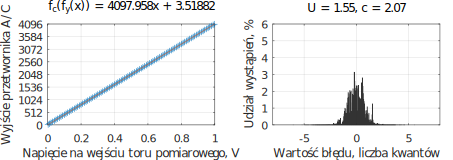
\includegraphics{obrazki/static_adcout}
\makecaption{fig:pom_static_fun}{Zależność wartości wielkości wyjściowej przetwornika analogowo-cyfrowego w funkcji wartości napięcia wejściowego analizowanego toru pomiarowego oraz histogram uzyskanych realizacji błędu losowego wielkości wyjściowej przetwornika analogowo-cyfrowego}
\end{center}
\end{figure}

Przeprowadzony eksperyment pozwolił na identyfikację wypadkowego błędu przesunięcia zera wzmacniacza pomiarowego oraz przetwornika analogowo cyfrowego dla wielkości $c(i)$, który w analizowanym przypadku wyniósł~\qty{3.52}{LSB}. Błąd ten korygowany jest na etapie odtwarzania wartości wielkości $x(i)$, w przypadku warunków otoczenia zbieżnych do panujących podczas przeprowadzania eksperymentu. Na podstawie dokumentacji zastosowanych komponentów w rozważaniach należy uwzględnić zależność realizacji omawianego sygnału błędu w funkcji temperatury otoczenia~\cite{microchip_manual, stm_f411, diodes_manual, stm_manual}. W przypadku wzmacniacza pomiarowego czułość błędu zera w funkcji temperatury otoczenia wynosi typowo $\pm (2 s_{y})~\unit{\micro V \per K}$ dla wzmocnienia statycznego $s_{y}$~\cite{microchip_manual}. W przypadku przetwornika analogowo-cyfrowego wartość ta nie jest przedstawiona w dokumentacji, natomiast producent układu proponuje wykonanie procedury kalibracji, a następnie na jej podstawie wykonywanie korekcji błędu przesunięcia zera stosując wbudowany przetwornik temperatury~\cite{stm_adc}. Omawiane zjawiska są również skorelowane z wpływem temperatury na wartość napięcia wyjściowego zastosowanych źródeł zasilających wymienione komponenty. W przypadku zmiany wartości temperatury otoczenia należy przeprowadzić odpowiedni eksperyment mający na celu identyfikację czułości sygnału błędu związanego z dryftem zera w funkcji temperatury otoczenia, a następnie korygować należy wyniki pomiaru lub uwzględniać udział omawianego sygnału błędu w budżecie niepewności~\cite{jcgm_guide}.

Analizując dokumentacje~\cite{microchip_manual, stm_manual, diodes_manual, stm_f411} kolejnych komponentów toru pomiarowego zauważyć można, że najistotniejsze źródło błędów związanych z właściwościami statycznymi stanowi w analizowanym przypadku przetwornik analogowo-cyfrowy. Zgodnie z dokumentacją~\cite{stm_f411}, typowa wartość błędu granicznego wielkości wyjściowej $c(i)$ dla zbliżonych do stosowanych w sporządzonej aplikacji parametrów pracy przetwornika analogowo-cyfrowego powinna mieścić się w przedziale \DIFdelbegin \DIFdel{$\pm<2; 3>~\unit{LSB}$}\DIFdelend \DIFaddbegin \DIFadd{$\pm \interval{2}{3}~\unit{LSB}$}\DIFaddend . Najważniejsze źródła \DIFdelbegin \DIFdel{błędu}\DIFdelend \DIFaddbegin \DIFadd{błędów}\DIFaddend , które zdefiniowane są przez producenta zastosowanego przetwornika analogowo-cyfrowego obejmują \DIFaddbegin \DIFadd{kolejno}\DIFaddend : błąd przesunięcia charakterystyki względem zera, \DIFaddbegin \DIFadd{różnicowy }\DIFaddend błąd \DIFdelbegin \DIFdel{wzmocnienia}\DIFdelend \DIFaddbegin \DIFadd{nieliniowości}\DIFaddend , całkowy błąd nieliniowości \DIFdelbegin \DIFdel{i różnicowy }\DIFdelend \DIFaddbegin \DIFadd{oraz }\DIFaddend błąd \DIFdelbegin \DIFdel{nieliniowości}\DIFdelend \DIFaddbegin \DIFadd{wzmocnienia}\DIFaddend ~\cite{stm_adc, stm_f411}. Uzyskana na drodze eksperymentu wartość niepewności rozszerzonej dla wypadkowego sygnału błędu wynikającego z przedstawionych źródeł błędów jest mniejsza od wartości wynikającej z opisanego w dokumentacji błędu granicznego i wynosi $U_{c,rw} = \qty{1.55}{LSB}$. Zależność ta wynika z faktu, że skorygowany został błąd zera oraz błąd wzmocnienia dla warunków otoczenia\DIFaddbegin \DIFadd{, }\DIFaddend w jakich przeprowadzano eksperyment. Należy zauważyć, że ze względu na niewielką w stosunku do rozdzielczości przetwornika liczbę serii pomiarowych, podczas eksperymentu nie udało się uzyskać większości realizacji różnicowego błędu nieliniowości. Na podstawie wyników eksperymentu oraz informacji zawartych w dokumentach~\cite{stm_f411, stm_adc} można jednak przyjąć, że wartość niepewności $U_{c,rw}$ została oszacowana prawidłowo. Ze względu na niewielką liczbę realizacji różnicowego błędu nieliniowości można zakładać, że rzeczywisty rozkład błędu $e_{c,rw}(i)$ będzie rozkładem normalnym, co wynika z centralnego twierdzenia granicznego~\cite{jcgm_guide}.

Drugą grupę właściwości obiektu stanowią właściwości dynamiczne. Podobnie, jak w przypadku właściwości statycznych, istnieje możliwość ich identyfikacji pomiarowej, uzyskując kolejne realizacje wielkości wyjściowej $c(i)$. Przypadek właściwości dynamicznych jest jednak złożony i wymaga stosowania bardziej skomplikowanej procedury pomiarów -- konieczna bowiem jest odpowiednia synchronizacja przebiegu napięcia wejściowego toru pomiarowego z przebiegiem sygnału wyjściowego przetwornika analogowo-cyfrowego, w celu oszacowania różnicy pomiędzy fazami analizowanych sygnałów. Opisywana procedura jest zatem kłopotliwa, a dodatkowo podczas jej realizacji wprowadzany byłby kolejny błąd, związany z opisywaną synchronizacją. Wobec powyższych okoliczności, proponuje się w pierwszej kolejności identyfikację właściwości dynamicznych zastosowanego wzmacniacza pomiarowego, a następnie ustalenie właściwości dynamicznych \DIFdelbegin \DIFdel{przetwornika analogowo-cyfrowego }\DIFdelend \DIFaddbegin \DIFadd{układu próbkująco-pamiętającego }\DIFaddend na podstawie jego dokumentacji~\cite{stm_f411}, która dostatecznie opisuje model tego \DIFdelbegin \DIFdel{przetwornika}\DIFdelend \DIFaddbegin \DIFadd{układu}\DIFaddend .

W przypadku wzmacniacza pomiarowego proponowana procedura identyfikacji jego właściwości dynamicznych polega na podawaniu na wejście analizowanego wzmacniacza napięcia sinusoidalnie zmiennego o zadanej pulsacji i stałej amplitudzie. Dla zadanych parametrów sygnału wejściowego $s(t)$ zmierzyć należy amplitudę sygnału wyjściowego $y(t)$ wzmacniacza, potrzebną do wyznaczenia jego wzmocnienia $K_{y}(\omega)$, oraz przesunięcie fazowe $\varphi_{y}(\omega)$ pomiędzy sygnałem wejściowym i wyjściowym. Pomiędzy omawianymi wielkościami zachodzą następujące relacje:
\begin{gather}
K_{y} \emb{\omega} = \frac{E_{wy} \emb{\omega}}{E_{we} \emb{\omega}} \label{eq:pom_dyn_amp}, \\
\varphi_{y} \emb{\omega} = \varphi_{wy} \emb{\omega} - \varphi_{we} \emb{\omega} = -\omega \cdot \Delta t \emb{\omega} \label{eq:pom_dyn_phi},
\end{gather}
gdzie w funkcji pulsacji $E_{wy}(\omega)$ jest amplitudą sygnału wyjściowego, $E_{we}(\omega)$ amplitudą sygnału wejściowego, $\varphi_{wy}(\omega)$ przesunięciem fazowym sygnału wyjściowego, $\varphi_{we}(\omega)$ przesunięciem fazowym sygnału wejściowego wzmacniacza, natomiast $\Delta t(\omega)$ opóźnieniem sygnału wyjściowego $y(t)$ względem sygnału wejściowego $s(t)$.

Omawiany eksperyment przeprowadzono wykorzystując \DIFdelbegin \DIFdel{jako źródło napięcia wejściowego $s(t)$ analizowanego wzmacniacza }\DIFdelend generator przebiegów arbitralnych RIGOL~DG1011~\cite{rigol_fawg}\DIFaddbegin \DIFadd{, jako źródło napięcia wejściowego $s(t)$ analizowanego wzmacniacza}\DIFaddend . W celu pomiaru wartości parametrów zawartych w równaniach~\eqref{eq:pom_dyn_amp} oraz~\eqref{eq:pom_dyn_phi} zastosowano oscyloskop RIGOL~DS5062MA~\cite{rigol_dso} w połączeniu z dwiema identycznymi sondami P6100~\cite{wellzion_probes}. Ze względu na zastosowanie dwóch identycznych sond\DIFdelbegin \DIFdel{pomiarowych }\DIFdelend \DIFaddbegin \DIFadd{, }\DIFaddend obecne w zmierzonym wzmocnieniu i przesunięciu fazowym błędy były identyczne dla obydwóch kanałów, a zatem w równaniach~\eqref{eq:pom_dyn_amp} oraz~\eqref{eq:pom_dyn_phi} wzajemnie się kompensowały. Ze względu na pomiar amplitudy sygnału zarówno dla napięcia wejściowego, jak i wyjściowego analizowanego wzmacniacza, ewentualna rozbieżność nastawy wartości amplitudy napięcia wyjściowego generatora była nieistotna. Ze względu na bardzo małą wartość błędu nastawy częstotliwości przyjmuje się, że rzeczywista wartość częstotliwości sygnału wyjściowego generatora jest równa wartości zadanej tej częstotliwości. Podczas pomiarów analizowano uśrednione wartości dla \DIFdelbegin \DIFdel{~}\DIFdelend \num{256} realizacji obserwowanych sygnałów, przy czym pomiary wykonano dla częstotliwości sygnału $s(t)$ w przedziale \DIFdelbegin \DIFdel{$\hat{f} \in~<\num{0.1};\num{250}>~\unit{kHz}$}\DIFdelend \DIFaddbegin \DIFadd{$\hat{f} \in \interval{\num{0.1}}{\num{250}}~\unit{kHz}$}\DIFaddend .

Na podstawie pozyskanych danych oszacowano pasmo przenoszenia analizowanego wzmacniacza, któremu dla zastosowanej konfiguracji układu odpowiadała częstotliwość graniczna $f_{y,g} \approx \qty{165}{kHz}$ oraz wzmocnienie statyczne $s_{y,a} \approx \qty{3.28}{V \per V}$. Dla uzyskanych charakterystyk sporządzono dwa modele aproksymacji, mające na celu przybliżenie właściwości analizowanego obiektu w zakresie częstotliwości \DIFdelbegin \DIFdel{$f \in~<0;\frac{1}{2}f_{p}>$}\DIFdelend \DIFaddbegin \DIFadd{$f \in \interval{0}{\frac{1}{2}f_{p}}$}\DIFaddend . W modelu pierwszym \DIFaddbegin \DIFadd{($a$) }\DIFaddend wykorzystano funkcję opisującą transmitancję wzmacniacza w postaci:
\begin{gather}
\tilde{G}_{y,a} \emb{j\omega} \approx \frac{s_{y,a}}{1 + j \frac{\omega}{2 \pi f_{y,g}}} = \frac{s_{y,a}}{\frac{\omega^{2}}{4 \pi^{2} f_{y,g}^{2}} + 1} - j \frac{\omega s_{y,a}}{2 \pi f_{y,g} \left( \frac{\omega^{2}}{4 \pi^{2} f_{y,g}^{2}} + 1 \right) } \label{eq:pom_dyn_trans},
\end{gather}
natomiast dla modelu drugiego \DIFaddbegin \DIFadd{($b$) }\DIFaddend wykonano metodą najmniejszych kwadratów aproksymacje wielkości opisanych równaniami~\eqref{eq:pom_dyn_amp} oraz~\eqref{eq:pom_dyn_phi} przy użyciu funkcji:
\begin{gather}
\tilde{K}_{y,b} \emb{\omega} \approx \num{3.28} \label{eq:pom_aprox_amp}, \\
\tilde{\varphi}_{y,b} \emb{\omega} \approx -\frac{\num{6.821}}{\num{e13}} \omega^{2} - \frac{\num{5.462}}{\num{e07}} \omega \label{eq:pom_aprox_phi}.
\end{gather}
Uzyskane dla sygnału o częstotliwościach z zakresu \DIFdelbegin \DIFdel{$\hat{f} \in~<\num{0.1};\num{48}>~\unit{kHz}$ }\DIFdelend \DIFaddbegin \DIFadd{$\hat{f} \in \interval{\num{0.1}}{\num{48}}~\unit{kHz}$ }\DIFaddend wartości wzmocnienia i przesunięcia fazowego oraz odpowiadające im aproksymacje dla modeli opisanych w równaniach od~\eqref{eq:pom_dyn_trans} do~\eqref{eq:pom_aprox_phi} przedstawiono na rysunku~\ref{fig:pom_dynamic_ampout}. Należy zauważyć, że w analizowanym przypadku dla częstotliwości sygnału wyższych od częstotliwości Nyquista\DIFaddbegin \DIFadd{, }\DIFaddend właściwości dynamiczne wzmacniacza pomiarowego są nieistotne, a zatem przedstawione w równaniach od~\eqref{eq:pom_dyn_trans} do~\eqref{eq:pom_aprox_phi} aproksymacje powinny być dokładne jedynie dla częstotliwości \DIFdelbegin \DIFdel{$\hat{f} \in~<\num{0.1};\num{24}>~\unit{kHz}$}\DIFdelend \DIFaddbegin \DIFadd{$\hat{f} \in \interval{\num{0.1}}{\num{24}}~\unit{kHz}$}\DIFaddend . W przypadku zmiany częstotliwości próbkowania należy zaproponować nowy model aproksymacji omawianych parametrów, odpowiedni dla wybranej częstotliwości próbkowania.

\begin{figure}[htb!]
\begin{center}
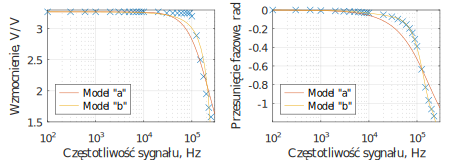
\includegraphics{obrazki/dynamic_ampout}
\makecaption{fig:pom_dynamic_ampout}{Zależność wartości wzmocnienia oraz przesunięcia fazowego w funkcji częstotliwości dla zastosowanej konfiguracji wzmacniacza pomiarowego}
\end{center}
\end{figure}

Analizując przedstawione wykresy zauważyć można, że model zaproponowany w równaniach~\eqref{eq:pom_aprox_amp} oraz~\eqref{eq:pom_aprox_phi} stanowi akceptowalne przybliżenie charakterystyki analizowanego wzmacniacza pomiarowego, natomiast model dany równaniem~\eqref{eq:pom_dyn_trans} odbiega od niej znacząco, przez co nie może być stosowany. Wobec powyższych przyjmuje się, że równania~\eqref{eq:pom_aprox_amp} oraz~\eqref{eq:pom_aprox_phi} opisują właściwości dynamiczne zastosowanego wzmacniacza, odpowiadające zależnościom~\eqref{eq:mid_cont_amp} oraz~\eqref{eq:mid_cont_phi}, a zatem zachodzi $\tilde{K}_{y}(\omega) = \tilde{K}_{y,b}(\omega)$ oraz $\tilde{\varphi}_{y}(\omega) = \tilde{\varphi}_{y,b}(\omega)$. Należy zauważyć, że na potrzeby zaproponowanego w pracy modelu błędów pozyskane w wyniku przeprowadzonego eksperymentu dane są wystarczające i nie jest konieczna znajomość dokładnej postaci funkcji opisującej transmitancję analizowanego obiektu. Jako, że zaproponowane modele stanowią jedynie przybliżenie wartości parametrów wynikających z rzeczywistych właściwości analizowanego wzmacniacza, a dodatkowo przeprowadzone pomiary były obarczone błędem wynikającym z przyjętej metodologii oraz właściwości przyrządu pomiarowego, rzeczywiste wartości parametrów amplitudy \DIFdelbegin \DIFdel{$\dot{K}_{y}(\omega)$ }\DIFdelend \DIFaddbegin \DIFadd{$\tilde{K}_{y}(\omega)$ }\DIFaddend oraz przesunięcia fazowego \DIFdelbegin \DIFdel{$\dot{\varphi}_{y}(\omega)$ }\DIFdelend \DIFaddbegin \DIFadd{$\tilde{\varphi}_{y}(\omega)$ }\DIFaddend będą najprawdopodobniej inne, niż oszacowane. Ze względu na właściwości zastosowanego oscyloskopu zakładać można niewielki błąd wyznaczania wartości fazy oraz znaczący błąd wyznaczania wartości wzmocnienia~\cite{rigol_dso}.

Ostatni etap identyfikacji właściwości dynamicznych obejmuje właściwości \DIFdelbegin \DIFdel{przetwornika analogowo-cyfrowego. Zgodnie z dokumentacją~\mbox{%DIFAUXCMD
\cite{stm_f411} }\hskip0pt%DIFAUXCMD
obwód zastępczy części analogowej }\DIFdelend \DIFaddbegin \DIFadd{układu próbkująco-pamiętającego. Na podstawie dokumentacji~\mbox{%DIFAUXCMD
\cite{stm_f411} }\hskip0pt%DIFAUXCMD
część analogową }\DIFaddend przetwornika analogowo-cyfrowego\DIFdelbegin \DIFdel{przedstawić }\DIFdelend \DIFaddbegin \DIFadd{, stanowiącą układ próbkująco-pamiętający, zastąpić }\DIFaddend można \DIFdelbegin \DIFdel{w postaci modelu }\DIFdelend \DIFaddbegin \DIFadd{modelem }\DIFaddend filtra dolno-przepustowego RC drugiego rzędu, co przedstawiono na rysunku~\ref{fig:pom_schemat_adc}. Wypadkowa pojemność $C_{we}$ \DIFaddbegin \DIFadd{układu }\DIFaddend wynika w analizowanym przypadku z pojemności w obrębie wyprowadzenia mikrokontrolera oraz pojemności obecnego na wyjściu wzmacniacza filtru RC, natomiast pojemność $C_{adc}$ wynika pojemności wewnętrznej układu próbkująco-pamiętającego. Zgodnie z dokumentacją~\cite{stm_f411} wewnętrzna pojemność \DIFdelbegin \DIFdel{przetwornika }\DIFdelend \DIFaddbegin \DIFadd{$C_{adc}$ }\DIFaddend wynosi typowo około~\qty{4}{pF}, natomiast pojemność zastępcza $C_{we}$ obwodu wejściowego przetwornika wynosi zwykle~\qty{5}{pF}. Rezystancję $R_{we}$ w zaproponowanym modelu stanowi szeregowe połączenie rezystancji doprowadzeń pomiędzy wzmacniaczem pomiarowym i mikrokontrolerem oraz rezystancji wyjściowej wzmacniacza. Rezystancja $R_{adc}$ odpowiada \DIFaddbegin \DIFadd{natomiast }\DIFaddend rezystancji klucza układu próbkująco-pamiętającego\DIFdelbegin \DIFdel{i, }\DIFdelend \DIFaddbegin \DIFadd{, gdzie }\DIFaddend zgodnie z dokumentacją~\cite{stm_f411} \DIFdelbegin \DIFdel{, }\DIFdelend jej wartość nie przekracza~\qty{6}{k\ohm}. Dodatkowe elementy, które można zauważyć na omawianym schemacie, to diody zabezpieczające wejście mikrokontrolera przed zbyt wysokim lub zbyt niskim napięciem wejściowym oraz źródło $I_{adc}$, które zastępuje upływność układu nieprzekraczającą~\qty{\pm 1}{\micro A}. Elementy te mogą być pominięte w omawianej analizie, ze względu na ich znikome znaczenie w budżecie błędów analizowanego toru pomiarowego.

Pierwszy filtr przedstawiony na rysunku~\ref{fig:pom_schemat_adc} składa się zatem z rezystancji $R_{we} \approx \qty{100}{\ohm}$ oraz pojemności $C_{we} \approx \qty{48}{nF}$, co wynika z parametrów impedancji wyjściowej wzmacniacza dla parametrów małosygnałowych~\cite{microchip_application} oraz zastosowanego na jego wyjściu filtru RC. Pozwala to oszacować częstotliwość graniczną tego filtru na poziomie~\qty{21}{MHz}, przy czym udział omawianego obiektu w przetwarzaniu sygnału $y(t)$ został już opisany podczas analizy właściwości dynamicznych wzmacniacza pomiarowego. Przedstawione rozważania zakładają pomijalnie małą impedancję wyjściową wzmacniacza dla parametrów małosygnałowych oraz pomijalny udział pojemności ścieżek w obrębie wejścia mikrokontrolera w porównaniu do parametrów zastosowanego filtru RC na wyjściu wzmacniacza.

\begin{figure}[htb!]
\begin{center}
\includegraphics{obrazki/schemat_adc}
\DIFdelbeginFL %DIFDELCMD < \makecaption{fig:pom_schemat_adc}{Schemat zastępczy modelu przetwornika analogowo-cyfrowego zastosowanego w analizowanym torze pomiarowym zgodny z dokumentacją producenta układu~\cite{stm_f411}}
%DIFDELCMD < %%%
\DIFdelendFL \DIFaddbeginFL \makecaption{fig:pom_schemat_adc}{Schemat zastępczy modelu przetwornika analogowo-cyfrowego zastosowanego w analizowanym torze pomiarowym, zgodny z dokumentacją producenta układu~\cite{stm_f411}}
\DIFaddendFL \end{center}
\end{figure}

W najmniej korzystnym przypadku\DIFaddbegin \DIFadd{, }\DIFaddend filtr drugi stanowi połączenie rezystancji $R_{adc} \approx \qty{6}{k \ohm}$ z pojemnością $C_{adc} \approx \qty{7}{pF}$~\cite{stm_f411}, a zatem rząd wielkości częstotliwości granicznej takiego filtru oszacować można na poziomie~\qty{24}{MHz}. Wobec powyższych, przyjąć można pomijalnie mały wpływ tego filtru na amplitudę przetwarzanego sygnału, natomiast uwzględnić należy wprowadzane przez niego przesunięcie fazowe. Proponuje się zatem oszacować przesunięcie fazowe sygnału $c(i)$ względem sygnału $y(t)$ w postaci:
\begin{equation}
\tilde{\varphi}_{c} \emb{\omega} \approx \arctan \emb{-\frac{\omega}{2\pi} R_{adc} C_{adc}} \label{eq:pom_adcin_phi},
\end{equation}
oraz przyjąć stałe wzmocnienie dla analizowanego fragmentu przetwornika równe jedności:
\begin{equation}
\tilde{K}_{c} \emb{\omega} \approx \qty{1}{V \per V} \label{eq:pom_adcin_amp}\DIFdelbegin \DIFdel{,
}\DIFdelend \DIFaddbegin \DIFadd{.
}\DIFaddend \end{equation}
Jako, że analizowany układ stanowi rozwiązanie typu \enquote{SoC}, rzeczywiste wartości parametrów $R_{adc}$ oraz $C_{adc}$ są niemożliwe do wyznaczenia. Na podstawie dokumentacji układu możliwe jest jedynie oszacowanie stałej czasowej omawianego filtru. Należy również zauważyć, że zintegrowany z przetwornikiem analogowo-cyfrowym układ próbkująco-pamiętający wprowadzać będzie do sygnału $c(i)$ dodatkowe opóźnienie względem sygnału $y(t)$ wynikające z czasu trwania stanu śledzenia, który w analizowanym przypadku wynosi $T_{sam} = \qty{12}{\micro s}$. Jako, że docelowo tor pomiarowy pracuje w trybie ciągłym, wpływ omawianego zjawiska nie jest istotny i można go odpowiednio skompensować, co przedstawiono w dalszej części rozdziału, a zatem zjawisko to nie jest uwzględniane w równaniu~\eqref{eq:pom_adcin_phi}.

Ostatnim fragmentem toru pomiarowego, który wprowadzać może do sygnału wyjściowego dodatkowe błędy, jest algorytm dyskretnej transformacji falkowej. Przeprowadzone wcześniej badania, których wyniki przedstawiono w tabeli~\ref{tab:varnum_spline4_4_5_f32}, pozwalają przypuszczać, że wariancja błędu związanego z zaokrągleniami nie przekroczy w bieżącym przypadku rzędu \DIFdelbegin \DIFdel{~}%DIFDELCMD < \unit{\pico V}%%%
\DIFdelend \DIFaddbegin \DIFadd{piko woltów}\DIFaddend , a zatem niepewność rozszerzona z nią związana nie powinna przekroczyć rzędu \DIFdelbegin \DIFdel{~}%DIFDELCMD < \unit{\micro V}%%%
\DIFdelend \DIFaddbegin \DIFadd{mikro woltów}\DIFaddend . Oznacza to, że błędy własne zastosowanego algorytmu dyskretnej transformacji falkowej mogą być pominięte w budżecie niepewności, bez większego wpływu na oszacowaną wartość niepewności rozszerzonej wielkości wyjściowych analizowanego toru pomiarowego~\cite{jcgm_guide}, a zatem ich udział nie został uwzględniony w przeprowadzonej analizie.

Należy zaznaczyć, że z punktu widzenia proponowanego modelu błędów dokładna znajomość postaci funkcji przetwarzania statycznego każdego elementu toru pomiarowego nie jest znana. Przykładowo, pomimo udziału funkcji przetwarzania $f_{y}(x)$ wzmacniacza pomiarowego w równaniach~\eqref{eq:pom_func_static} oraz~\eqref{eq:pom_funx_static}, znajomość tej funkcji nie jest konieczna podczas omawianej analizy. Dodatkowo na podstawie treści przedstawionych równań zauważyć można, że na etapie przetwarzania wielkości $c(i)$ wprowadzane jest przesunięcie charakterystyki statycznej, spowodowane błędem zera wzmacniacza pomiarowego i przetwornika analogowo-cyfrowego. Opisywana sytuacja powoduje, że funkcja przetwarzania nie spełnia właściwości addytywności, przez co nie jest możliwa analiza każdego sygnału błędu z osobna, jak proponowano w opisanym w pracy modelu błędów. Przeprowadzenie analizy z punktu widzenia wielkości wejściowej algorytmu dyskretnej transformacji falkowej umożliwia eliminację opisywanych niedogodności i wykorzystanie równań od~\eqref{eq:out_disc_err_stat_self} do~\eqref{eq:out_disc_err_rand_prop}, umożliwiających analizę z zastosowaniem metody superpozycji dla zdefiniowanych sygnałów błędów.

Zaproponowany algorytm identyfikacji właściwości metrologicznych analizowanego fragmentu toru pomiarowego jest wystarczający w celu aplikacji sporządzonego w ramach pracy modelu błędów. Jako, że parametry te zostały jedynie oszacowane, wyznaczone na ich podstawie wartości niepewności rozszerzonych wielkości wyjściowych toru pomiarowego mogą być obarczone pewnym błędem wynikającym z niedokładności wyznaczenia parametrów modelu błędów. Znacznie dokładniejszym sposobem na przeprowadzenie omawianej identyfikacji byłoby wykonanie symulacji z użyciem odpowiedniego oprogramowania, np. \enquote{LTspice}, czy \enquote{NGSpice}~\cite{mikkelsen_ltspice, nenzi_ngspice}. Przedstawioną metodologię zaproponowano z uwagi na fakt, że jest ona uniwersalna i nie wymaga konieczności znajomości dokładnego modelu stosowanych układów.

\section{Model błędów toru pomiarowego}

Przyjmując założoną wcześniej czułość dla wielkości $x(i)$ w stosunku do przetwarzanego sygnału $s(t)$ równą $s_{s,x} = \qty{1}{V \per V}$, idealny oraz zakłócony sygnałem błędu przebieg wielkości $x(i)$ opisać można w postaci:
\begin{gather}
\dot{x} \emb{i} = s_{s,x} \dot{s} \DIFdelbegin %DIFDELCMD < \emb{kT_{p}} %%%
\DIFdelend \DIFaddbegin \emb{iT_{p}} \DIFaddend = \dot{s} \emb{kT_{p}} \label{eq:pom_dwtin_ideal}, \\
\tilde{x} \emb{i} = \dot{s} \DIFdelbegin %DIFDELCMD < \emb{kT_{p}} %%%
\DIFdelend \DIFaddbegin \emb{iT_{p}} \DIFaddend + e_{x,\Sigma} \emb{i} \label{eq:pom_dwtin_real},
\end{gather}
przy czym składowe sygnału błędu $e_{x,\Sigma}(i)$ opisano w dalszej części podrozdziału. Zgodnie z równaniami~\eqref{eq:mid_disc_sum_real} oraz~\eqref{eq:out_disc_real_all}, w przypadku sygnału $s(t)$ o charakterze deterministycznym, którego kolejne harmoniczne mogą być opisane postaci równania:
\begin{equation}
\tilde{s}(t,\omega) = E_{s}(\omega) \sin(\omega t + \varphi_{s}(\omega)) \label{eq:pom_dwtin_harm_ideal},
\end{equation}
rzeczywisty przebieg wybranej harmonicznej sygnału $x(i)$ stanowiącego wejście algorytmu transformacji falkowej opisać można w postaci:
\begin{equation}
\tilde{x} \emb{i,\omega} =  s_{s,x} \sum\DIFdelbegin \DIFdel{_{k = 0} }\DIFdelend \DIFaddbegin \DIFadd{_{j = 0} }\DIFaddend ^{\infty} \tilde{K}_{s,x} \DIFdelbegin %DIFDELCMD < \emb{\omega_{k}} %%%
\DIFdelend \DIFaddbegin \emb{\omega_{s,j}} \DIFaddend E_{s} \DIFdelbegin %DIFDELCMD < \emb{\omega_{k}} %%%
\DIFdelend \DIFaddbegin \emb{\omega_{s,j}} \DIFaddend \sin \DIFdelbegin %DIFDELCMD < \emb{\omega_{k} i T_{p} + \varphi_{s}(\omega_{k}) + \tilde{\varphi}_{s,x} \emb{\omega_{k}}} %%%
\DIFdelend \DIFaddbegin \emb{\omega_{s,j} i T_{p} + \varphi_{s}(\omega_{s,j}) + \tilde{\varphi}_{s,x} \emb{\omega_{s,j}}} \DIFaddend \label{eq:pom_dwtin_harmsum}.
\end{equation}
Wariancję sygnału $x(i)$ na wejściu algorytmu transformacji falkowej w funkcji pulsacji opisać można w przypadku przetwarzanego sygnału $s(t)$ na podstawie równań~\DIFdelbegin \DIFdel{\eqref{eq:mid_disc_err_sum_all} }\DIFdelend \DIFaddbegin \DIFadd{\eqref{eq:mid_disc_var_omega} }\DIFaddend oraz~\eqref{eq:out_disc_var_sense} jako:
\begin{equation}
\sigma_{x}^{2} \emb{\omega} = s_{s,x}^{2} \tilde{K}_{s,x}^{2} \emb{\omega} \sigma\DIFdelbegin \DIFdel{_{y}}\DIFdelend \DIFaddbegin \DIFadd{_{s}}\DIFaddend ^{2} \emb{\omega} \label{eq:pom_dwtin_var},
\end{equation}
gdzie \DIFdelbegin \DIFdel{$\sigma_{y}^{2}(\omega)$ }\DIFdelend \DIFaddbegin \DIFadd{$\sigma_{s}^{2}(\omega)$ }\DIFaddend jest wariancją sygnału $s(t)$. Zależność~\eqref{eq:pom_dwtin_var} jest odpowiednia zarówno w przypadku sygnałów deterministycznych, jak i niedeterministycznych.

Wartość wzmocnienia \DIFdelbegin \DIFdel{$\tilde{K}_{s,x}(\omega)$ }\DIFdelend \DIFaddbegin \DIFadd{$K_{s,x}(\omega)$ }\DIFaddend jest wypadkową wartością wzmocnienia uzyskaną dla kaskadowego połączenia wzmacniacza pomiarowego, którego wzmocnienie oznaczono symbolem \DIFdelbegin \DIFdel{$\tilde{K}_{y}(\omega)$}\DIFdelend \DIFaddbegin \DIFadd{$K_{y}(\omega)$}\DIFaddend , przetwornika analogowo-cyfrowego, którego wzmocnienie oznaczono jako \DIFdelbegin \DIFdel{$\tilde{K}_{c}(\omega)$ }\DIFdelend \DIFaddbegin \DIFadd{$K_{c}(\omega)$ }\DIFaddend oraz algorytmu odtwarzania statycznego, którego nieomówione dotychczas wzmocnienie oznaczono symbolem \DIFdelbegin \DIFdel{$\tilde{K}_{x}(\omega)$}\DIFdelend \DIFaddbegin \DIFadd{$K_{x}(\omega)$}\DIFaddend . Wobec powyższych założeń zapisać można:
\begin{equation}
\DIFdelbegin %DIFDELCMD < \tilde{K}%%%
\DIFdelend \DIFaddbegin \DIFadd{K}\DIFaddend _{s,x} \emb{\omega} = \DIFdelbegin %DIFDELCMD < \tilde{K}%%%
\DIFdelend \DIFaddbegin \DIFadd{K}\DIFaddend _{y} \emb{\omega} \DIFdelbegin %DIFDELCMD < \tilde{K}%%%
\DIFdelend \DIFaddbegin \DIFadd{K}\DIFaddend _{c} \emb{\omega} \DIFdelbegin %DIFDELCMD < \tilde{K}%%%
\DIFdelend \DIFaddbegin \DIFadd{K}\DIFaddend _{x} \emb{\omega} \DIFdelbegin %DIFDELCMD < \label{eq:pom_dwtin_amp}%%%
\DIFdelend \DIFaddbegin \label{eq:pom_dwtin_amp_mul}\DIFaddend ,
\end{equation}
przy czym zgodnie z założeniami dotyczącymi postaci funkcji odtwarzania, opisanej równaniem~\eqref{eq:pom_funx_static} oraz założeń danych równaniem~\eqref{eq:pom_dwtin_ideal} odnośnie jednostkowej czułości sygnału $x(i)$ względem sygnału $s(t)$, dla których zachodzi \DIFdelbegin \DIFdel{$\tilde{K}_{s,x}(0) = \qty{1}{V \per V}$}\DIFdelend \DIFaddbegin \DIFadd{$\dot{K}_{s,x}(\omega) = \qty{1}{V \per V}$}\DIFaddend , wartość wzmocnienia \DIFdelbegin \DIFdel{$\tilde{K}_{x}(\omega)$ }\DIFdelend \DIFaddbegin \DIFadd{$K_{x}(\omega)$ }\DIFaddend jest wartością stałą i kompensuje ona wzmocnienie statyczne wzmacniacza oraz przetwornika analogowo-cyfrowego, a zatem może ona być opisana równaniem:
\begin{equation}
\DIFdelbegin %DIFDELCMD < \tilde{K}%%%
\DIFdelend \DIFaddbegin \DIFadd{K}\DIFaddend _{x} \emb{\omega} = \DIFdelbegin \DIFdel{\frac{1}{\tilde{K}_{y} \emb{0} \tilde{K}_{c} \emb{0}} \approx \frac{1}{\num{3.28}}~}%DIFDELCMD < \unit{V \per V} %%%
\DIFdelend \DIFaddbegin \DIFadd{\frac{1}{K_{y} \emb{0} K_{c} \emb{0}} }\DIFaddend \label{eq:pom_dwtin_ampnorm},
\end{equation}
\DIFdelbegin \DIFdel{przy czym zgodnie z }\DIFdelend \DIFaddbegin \DIFadd{gdzie w analizowanym przypadku $\tilde{K}_{x}(\omega) \approx \frac{1}{\num{3.28}}~\unit{V \per V}$. Ostatecznie, zgodnie założeniem danym równaniem~\eqref{eq:pom_dwtin_ideal}, }\DIFaddend treścią równań~\eqref{eq:pom_aprox_amp}\DIFdelbegin \DIFdel{oraz~\eqref{eq:pom_adcin_amp} }\DIFdelend \DIFaddbegin \DIFadd{, \eqref{eq:pom_adcin_amp}, \eqref{eq:pom_dwtin_amp_mul} oraz~\eqref{eq:pom_dwtin_ampnorm}, }\DIFaddend przyjąć można\DIFdelbegin \DIFdel{, że $\tilde{K}_{x}(\omega) \approx \qty{1}{V \per V}$. Dla przypadku idealnego zakłada się stałe jednostkowe wzmocnienie dynamiczne, a zatem zachodzi:
}\DIFdelend \DIFaddbegin \DIFadd{:
}\DIFaddend \begin{equation}
\DIFdelbegin %DIFDELCMD < \dot{K}%%%
\DIFdelend \DIFaddbegin \tilde{K}\DIFaddend _{s,x}(\omega) \DIFaddbegin \DIFadd{\approx }\dot{K}\DIFadd{_{s,x} }\emb{\omega} \DIFaddend = \qty{1}{V \per V} \DIFdelbegin %DIFDELCMD < \label{eq:pom_dwtin_ampideal}%%%
\DIFdelend \DIFaddbegin \label{eq:pom_dwtin_amp}\DIFaddend .
\end{equation}

Przesunięcie fazowe $\tilde{\varphi}_{s,x}(\omega)$ sygnału $x(i)$ względem sygnału $s(t)$, wynikające z przesunięcia $\tilde{\varphi}_{y}(\omega)$ wprowadzanego przez wzmacniacz oraz wprowadzanego przez przetwornik analogowo-cyfrowy przesunięcia \DIFdelbegin \DIFdel{$\tilde{\varphi}_{s,x}(\omega)$ }\DIFdelend \DIFaddbegin \DIFadd{$\tilde{\varphi}_{c}(\omega)$, }\DIFaddend opisać można jako:
\begin{equation}
\tilde{\varphi}_{s,x} \emb{\omega} = \tilde{\varphi}_{y} \emb{\omega} + \tilde{\varphi}\DIFdelbegin \DIFdel{_{s,x} }\DIFdelend \DIFaddbegin \DIFadd{_{c} }\DIFaddend \emb{\omega} \approx -\frac{\num{6.821}}{\num{e13}} \omega^{2} - \frac{\num{5.462}}{\num{e07}} \omega - \arctan \emb{\frac{\num{6.685}}{\num{e9}} \omega} \label{eq:pom_dwtin_phi},
\end{equation}
co wynika z równań~\eqref{eq:pom_aprox_phi} oraz~\eqref{eq:pom_adcin_phi}. W rozważaniach nie uwzględniono przesunięcia fazowego wprowadzanego przez algorytm odtwarzania statycznego, ponieważ algorytm ten nie wprowadza żadnego przesunięcia w fazie dla przetwarzanego sygnału. Przyjmuje się, że w przypadku idealnym sygnał $x(i)$ powinien cechować się fazą identyczną, jak przetwarzany sygnał $s(t)$, zatem \DIFaddbegin \DIFadd{zapisać można}\DIFaddend :
\begin{equation}
\dot{\varphi}_{s,x}(\omega) = \qty{0}{rad} \label{eq:pom_dwtin_phiideal}.
\end{equation}

Pierwszy składnik zawarty w sygnale błędu $e_{x,\Sigma}(i)$ stanowi sygnał $e_{x,rw}(i)$ związany ze zidentyfikowanymi właściwościami statycznymi analizowanego fragmentu toru pomiarowego, stanowiącego źródło danych algorytmu transformacji falkowej, opisany dla warunków wykonanego eksperymentu równaniem~\eqref{eq:pom_funx_error}. Jako, że deterministyczna postać omawianego sygnału błędu nie jest znana oraz wartości jego realizacji nie zależą od częstotliwości przetwarzanego sygnału, przyjmuje się, że sygnał ten zalicza się do zbioru błędów losowych własnych. Niepewność rozszerzona związana z omawianym sygnałem błędu wynosi, zgodnie z poprzednimi rozważaniami, $U_{x,rw} = \qty{0.62}{mV}$ oraz przyjmuje się normalny rozkład realizacji tego sygnału\DIFaddbegin \DIFadd{, zatem współczynnik rozszerzenia $c_{x,rw}$ jest równy }\num{1.96}\DIFadd{~\mbox{%DIFAUXCMD
\cite{jcgm_guide}}\hskip0pt%DIFAUXCMD
}\DIFaddend .

Drugi składnik sygnału błędu $e_{x,\Sigma}(i)$ stanowi sygnał związany z właściwościami dynamicznymi wzmacniacza pomiarowego oraz przetwornika analogowo-cyfrowego, przy czym błąd ten ma charakter deterministyczny i można podzielić go na sygnał związany z błędem własnym $e_{x,dw}(i)$ oraz propagowanym $e_{x,dp}(i)$. Analizując założenie związane z równaniem~\eqref{eq:pom_dwtin_amp}, gdzie przyjęto $\tilde{K}_{s,x}(\omega) \approx \qty{1}{V \per V}$, zgodnie z równaniami~\eqref{eq:mid_disc_err_dyn_self}, \eqref{eq:mid_disc_err_dyn_prop}, \eqref{eq:pom_dwtin_ideal}, \eqref{eq:pom_dwtin_amp}, \eqref{eq:pom_dwtin_phi} oraz założeniem opisanym równaniem~\eqref{eq:pom_dwtin_phiideal} zachodzi:
\begin{gather}
\DIFdelbegin %DIFDELCMD < \begin{split}
%DIFDELCMD < e_{x,dw} \emb{i} =~
%DIFDELCMD < & \sum _{j = 1} ^{\infty} E_{s,o} \emb{\omega_{x,j}} \sin \left( \omega_{s,j} iT_{p} + \varphi_{s,o} \emb{\omega_{s,j}} + \tilde{\varphi}_{s,x} \emb{\omega_{s,j}} \right) - \\
%DIFDELCMD < & \sum _{k = 1} ^{\infty} E_{s,o} \emb{\omega_{x,k}} \sin \left( \omega_{s,k} iT_{p} + \varphi_{s,o} \emb{\omega_{s,k}} + \dot{\varphi}_{s,x} \emb{\omega_{s,k}} \right)
%DIFDELCMD < \end{split}%%%
\DIFdelend \DIFaddbegin \begin{split}
e_{x,dw} \emb{i} =~
& \sum _{j = 1} ^{\infty} E_{s,o} \emb{\omega_{s,j}} \sin \left( \omega_{s,j} iT_{p} + \varphi_{s,o} \emb{\omega_{s,j}} + \tilde{\varphi}_{s,x} \emb{\omega_{s,j}} \right) - \\
& \sum _{j = 1} ^{\infty} E_{s,o} \emb{\omega_{s,j}} \sin \left( \omega_{s,j} iT_{p} + \varphi_{s,o} \emb{\omega_{s,j}} + \dot{\varphi}_{s,x} \emb{\omega_{s,j}} \right)
\end{split}\DIFaddend 
\label{eq:pom_errx_dyn_self}, \\
e_{x,dp} \emb{i} = \sum _{j = 1} ^{\infty} E_{s,e} \emb{\omega_{s,j}} \sin \left( \omega_{s,j} iT_{p} + \varphi_{s,e} \emb{\omega_{s,j}} + \tilde{\varphi}_{s,x} \emb{\omega_{s,j}} \right) \label{eq:pom_errx_dyn_prop}.
\end{gather}

Trzeci składnik sygnału błędu $e_{x,\Sigma}(i)$ wynika z wpływu analizowanego obiektu na obecny w przetwarzanym sygnale $s(t)$ sygnał błędu statycznego \DIFdelbegin \DIFdel{$e_{s,s}(i)$}\DIFdelend \DIFaddbegin \DIFadd{$e_{s,s}(t)$}\DIFaddend , przy czym przebieg tego sygnału na wyjściu obiektu opisać można zgodnie z \DIFdelbegin \DIFdel{równaniem~\eqref{eq:out_disc_err_stat_prop}jako:
}\DIFdelend \DIFaddbegin \DIFadd{równaniami~\eqref{eq:mid_disc_err_stat_prop} oraz~\eqref{eq:out_disc_err_stat_prop}, gdzie:
}\DIFaddend \begin{equation}
e_{x,sp} \emb{i} \DIFdelbegin \DIFdel{= }\DIFdelend \DIFaddbegin \DIFadd{\cong }\DIFaddend e_{s,s} \emb{i T_{p}} \label{eq:pom_errx_stat_prop},
\end{equation}
a zatem, zgodnie z zależnościami~\eqref{eq:mid_disc_var_omega} oraz~\eqref{eq:out_disc_var_sense}, wariancję tego sygnału opisuje równanie:
\begin{equation}
\sigma_{x,sp}^{2} = s_{s,x}^{2} \tilde{K}_{s,x}^{2} \emb{0} \sigma_{s,s}^{2} \cong \sigma_{s,s}^{2} \label{eq:pom_varx_stat_prop}.
\end{equation}

Czwartym składnikiem sygnału błędu $e_{x,\Sigma}(i)$ jest propagowany sygnał błędu losowego $e_{x,rp}(i)$ związany z sygnałem \DIFdelbegin \DIFdel{$e_{s,r}(i)$}\DIFdelend \DIFaddbegin \DIFadd{$e_{s,r}(t)$}\DIFaddend . Zgodnie z zależnościami~\eqref{eq:mid_disc_var_omega} oraz~\eqref{eq:out_disc_var_sense} dla założenia danego równaniem~\eqref{eq:pom_dwtin_amp} wariancję tego sygnału opisać można w postaci:
\begin{equation}
\sigma_{x,rp}^{2} \emb{\omega} = s_{s,x}^{2} \tilde{K}_{s,x}^{2} \emb{\omega} \sigma_{s,r}^{2} \emb{\omega} \cong \sigma_{s,r}^{2} \emb{\omega} \label{eq:pom_varx_rand_prop_omega},
\end{equation}
co przy założeniu~\eqref{eq:pom_dwtin_ideal} odnośnie charakterystyki przetwarzania tego obiektu oznacza, że obiekt ten nie ma wpływu na postać przetwarzanych sygnałów losowych, a zatem \DIFaddbegin \DIFadd{przyjąć można uproszczenie}\DIFaddend :
\begin{equation}
e_{x,rp} \emb{i} \cong e_{s,r} \emb{i T_{p}} \label{eq:pom_errx_rand_prop}.
\end{equation}
Wobec powyższych założeń, dla sygnałów błędów losowych o stałej widmowej gęstości mocy, zapisać można:
\begin{equation}
\sigma_{x,rp}^{2} \cong \sigma_{s,r}^{2} \label{eq:pom_varx_rand_prop},
\end{equation}
gdzie podane równanie jest odpowiednie dla zakresu częstotliwości \DIFdelbegin \DIFdel{$\hat{f} \in~<0;\frac{1}{2} f_{p}>$}\DIFdelend \DIFaddbegin \DIFadd{$\hat{f} \in \interval{0}{\frac{1}{2} f_{p}}$}\DIFaddend .

Jako, że przeprowadzone eksperymenty wykonano przy stałych parametrach otoczenia, nie obejmowały one identyfikacji źródeł i postaci sygnału błędu statycznego własnego. Przyjmuje się zatem, że $e_{x,sw}(i) = 0$ oraz $\sigma_{x,sw}^{2} = \qty{0}{V}$. Na podstawie zależności od~\eqref{eq:pom_errx_dyn_self} do~\eqref{eq:pom_errx_rand_prop} wypadkowy sygnał błędu $e_{x,\Sigma}(i)$ opisać można jako sumę zdefiniowanych dotychczas sygnałów błędów cząstkowych w postaci:
\begin{equation}
e_{x,\Sigma} \emb{i} = e_{x,sp} \emb{i} + e_{x,dw} \emb{i} + e_{x,dp} \emb{i} + e_{x,rw} \emb{i} + e_{x,rp} \emb{i} \label{eq:pom_errx_sum},
\end{equation}
przy czym wypadkowe sygnały błędów z uwzględnieniem podziału na zaproponowane kategorie można zdefiniować jako:
\begin{gather}
e_{x,s} \emb{i} = e_{x,sp} \emb{i} \label{eq:pom_errx_stat}, \\
e_{x,r} \emb{i} = e_{x,rw} \emb{i} + e_{x,rp} \emb{i} \label{eq:pom_errx_rand}, \\
e_{x,d} \emb{i} = e_{x,dw} \emb{i} + e_{x,dp} \emb{i} = \sum _{j=1} ^{\infty} E_{x,e} \emb{\omega_{x,j}} \sin \DIFdelbegin %DIFDELCMD < \emb{i T_{p} \omega_{x,j} + \varphi_{x,e} \emb{\omega_{x,j}}} %%%
\DIFdelend \DIFaddbegin \emb{\omega_{x,j} iT_{p} + \varphi_{x,e} \emb{\omega_{x,j}}} \DIFaddend \label{eq:pom_errx_dyn},
\end{gather}
gdzie wypadkowe parametry amplitudy $E_{x,e}(\omega_{x,j})$ oraz fazy $\varphi_{x,e}(\omega_{x,j})$ dla kolejnych harmonicznych sygnału wypadkowego błędu dynamicznego $e_{x,d}(i)$ zależne będą od widma przetwarzanego sygnału, natomiast ich wyznaczenie przebiegać będzie zgodnie z metodologią opisaną w równaniach od~\eqref{eq:dyn_vect} do~\eqref{eq:dyn_vect_phi}. Wariancję kolejnych harmonicznych sygnału $e_{x,d}(i)$ wyznaczyć można zgodnie z zależnością~\eqref{eq:dyn_var}.

W przypadku sygnałów błędów statycznych dla $i$-tej wielkości wyjściowej toru pomiarowego wariancję sygnału błędu statycznego tej wielkości opisać można\DIFaddbegin \DIFadd{, }\DIFaddend zgodnie z równaniem~\eqref{eq:alg_outvar_stat}\DIFaddbegin \DIFadd{, }\DIFaddend jako:
\begin{equation}
\sigma_{i,s}^{2} = A_{i,s}^{2} \emb{\sigma_{x,sw}^{2} + \sigma_{x,sp}^{2}} = A_{i,s}^{2} \sigma_{s,s}^{2} = A_{i,s}^{2} \sigma_{x,s}^{2} \label{eq:pom_varout_stat}.
\end{equation}
Ze względu na stałą widmową gęstość mocy sygnału błędu losowego $e_{x,r}(i)$, wynikającą z przyjętych założeń odnośnie modelu sygnału szumu, błędu kwantowania oraz postaci wzmocnienia $\tilde{K}_{s,x}(\omega)$, wariancja sygnałów błędów losowych na wyjściu algorytmu może być opisana dla $i$-tej wielkości wyjściowej jako:
\begin{equation}
\sigma_{i,r}^{2} = A_{i,r}^{2} \emb{\sigma_{x,rw}^{2} + \sigma_{x,rp}^{2}} = A_{i,r}^{2} \emb{\sigma_{x,rw}^{2} + \sigma_{s,rw}^{2}} = A_{i,r}^{2} \sigma_{x,r}^{2} \label{eq:pom_varout_rand}.
\end{equation}
Jeżeli niespełnione zostaną założenia dotyczące stałej widmowej gęstości mocy sygnałów błędów losowych, należy zastosować równanie~\eqref{eq:mid_disc_var_omega} do wyznaczenia wariancji tych sygnałów na wyjściu algorytmu.
Dla sygnałów błędów dynamicznych wariancję tych sygnałów w funkcji pulsacji opisać można\DIFaddbegin \DIFadd{, }\DIFaddend zgodnie z zależnością~\eqref{eq:alg_outvar_dyn}\DIFaddbegin \DIFadd{, }\DIFaddend jako:
\begin{equation}
\sigma_{i,d}^{2} \emb{\omega} = \left| H_{i} \emb{e^{j \omega T_{p}}} \right|^{2} \sigma_{x,d}^{2} \emb{\omega} \label{eq:pom_varout_dyn},
\end{equation}
gdzie $H_{i}(e^{j \omega T_{p}})$ jest transmitancją \DIFaddbegin \DIFadd{związaną z }\DIFaddend $i$\DIFdelbegin \DIFdel{-tej wielkości wyjściowej algorytmu}\DIFdelend \DIFaddbegin \DIFadd{-tą wielkością wyjściową algorytmu, }\DIFaddend opisaną równaniem~\eqref{eq:alg_trans_single}. Wypadkowa wariancja sygnału błędu dynamicznego $e_{x,d}(i)$ może \DIFaddbegin \DIFadd{zatem }\DIFaddend zostać wyrażona w postaci sumy wypadkowych wariancji wszystkich harmonicznych tego sygnału, co opisuje równanie:
\begin{equation}
\sigma_{i,d}^{2} = \sum _{k=1} ^{\infty} \left| H_{i} \emb{e^{j \omega_{x,k} T_{p}}} \right|^{2} \sigma_{x,d}^{2} \emb{\omega_{x,k}} \label{eq:pom_varout_dyn_sum}.
\end{equation}
Należy zauważyć, że na etapie analizy kolejnych harmonicznych sygnału błędu dynamicznego $e_{x,d}(i)$ kolejne składowe tego sygnału o jednakowych pulsacjach mogą być ze sobą skorelowane. Proponowane w równaniu~\eqref{eq:pom_errx_dyn} przedstawienie tego sygnału w postaci kolejnych harmonicznych o parametrach wypadkowych umożliwia rozpatrzenie tych korelacji przy jednoczesnej redukcji liczby składowych analizowanego sygnału.

Ze względu na fakt, że przeprowadzona identyfikacja właściwości metrologicznych dla fragmentu toru pomiarowego związanego z wielkościami wejściowymi analizowanego algorytmu nie wykazała innych korelacji pomiędzy zidentyfikowanymi sygnałami błędów, zgodnie z równaniem~\eqref{eq:var_matrix} zapisać można:
\begin{equation}
\sigma_{i,\Sigma}^{2} = \sigma_{i,s}^{2} + \sigma_{i,d}^{2} + \sigma_{i,r}^{2} \label{eq:pom_varout_sum}.
\end{equation}
Wartości wariancji sygnałów propagowanego błędu statycznego, propagowanego błędu losowego oraz wypadkowego błędu dynamicznego nie są znane na obecnym etapie analizy. Dla wymienionych sygnałów wartość wariancji zależeć będzie od widma sygnału $s(t)$ oraz zawartych w nim sygnałów błędów.

Wartości niepewności rozszerzonych związane z wymienionymi sygnałami błędów na wyjściu algorytmu mogą być w analizowanej sytuacji opisane jako:
\begin{gather}
U_{i,s} = c_{i,s} \sigma_{i,s} = c_{s,s} A_{i,s} \sigma_{s,s} \label{eq:pom_uncout_stat}, \\
U_{i,r} = c_{i,r} \sigma_{i,r} = c_{n} \sqrt{\sigma_{x,rw}^{2} + \sigma_{s,rw}^{2}} \label{eq:pom_uncout_rand}, \\
U_{i,d,j} = c_{i,d,j} \sigma_{i,d} \emb{\omega_{x,j}} = c_{d} \sigma_{i,d} \emb{\omega_{x,j}} \label{eq:pom_uncout_dyn}.
\end{gather}
Wartość współczynnika rozszerzenia $c_{i,s} = c_{s,s} = c_{u} = \num{1.65}$ dla sygnału błędu statycznego wynika z założenia liniowości wszystkich fragmentów toru pomiarowego oraz występowania tylko jednego źródła sygnału błędu statycznego. Wartość współczynnika rozszerzenia $c_{i,r} = c_{n} = \num{1.96}$ w przypadku sygnału błędu losowego na wyjściu obiektu wynika z założeń centralnego twierdzenia granicznego, gdzie analizowany algorytm przetwarza wiele nieskorelowanych ze sobą sygnałów błędów losowych o jednakowych parametrach, a zatem rozkład realizacji tego sygnału jest rozkładem normalnym~\cite{jcgm_guide}. W przypadku kolejnych harmonicznych sygnału błędu dynamicznego współczynnik rozszerzenia wynika z kształtu rozkładu funkcji \enquote{sinus}. Należy zauważyć, że dla sygnału poliharmonicznego rozkład realizacji wypadkowego sygnału błędu dynamicznego będzie rozkładem o nietypowym kształcie, wynikającym ze złożenia określonej liczby harmonicznych sygnału błędu dynamicznego.

Wobec powyższych, wypadkowa wartość niepewności rozszerzonej na wyjściu algorytmu dla $i$-tej wielkości wyjściowej może być opisana zgodnie z równaniem~\eqref{eq:unc_matrix}, przy czym wektor niepewności rozszerzonych \DIFdelbegin \DIFdel{opisać można w postaci:
}\begin{displaymath}
\DIFdel{\mathbf{U}_{i}^{T} =
\begin{bmatrix}
U_{i,s} & U_{i,r} & U_{i,d,1} & U_{i,d,2} & \hdots & U_{i,d,K}
\end{bmatrix}
\label{eq:pom_uncout_uncvect},
}\end{displaymath}%DIFAUXCMD
\DIFdel{natomiast macierz koherencji }\DIFdelend dla $K$ harmonicznych sygnału błędu dynamicznego opisać można w postaci:
\DIFaddbegin \begin{equation}
\DIFadd{\mathbf{U}_{i} =
\begin{bmatrix}
U_{i,s} & U_{i,r} & U_{i,d,1} & U_{i,d,2} & \hdots & U_{i,d,K}
\end{bmatrix}
\label{eq:pom_uncout_uncvect},
}\end{equation}
\DIFadd{natomiast macierz koherencji przyjmuje w omawianym przypadku postać:
}\DIFaddend \begin{equation}
\mathbf{h}_{i} =
\begin{bmatrix}
1           & h_{i,s,r}   & h_{i,s,d,1} & h_{i,s,d,2} & \cdots & h_{i,s,d,K} \\
h_{i,r,s}   & 1           & h_{i,r,d,1} & h_{i,r,d,2} & \cdots & h_{i,r,d,K} \\
h_{i,d,1,s} & h_{i,d,1,r} & 1           & h_{i,d,1,2} & \cdots & h_{i,d,1,K} \\
h_{i,d,2,s} & h_{i,d,2,r} & h_{i,d,2,1} & 1           & \cdots & h_{i,d,2,K} \\
\vdots      &             &             &             & \ddots & \vdots      \\
h_{i,d,K,1} & \cdots      & \cdots      & \cdots      & \cdots & 1           \\
\end{bmatrix}
\label{eq:pom_uncout_cohers},
\end{equation}
gdzie kolejne wartości \DIFaddbegin \DIFadd{wymienionych }\DIFaddend współczynników koherencji są wyznaczane zgodnie z równaniem~\eqref{eq:unc_coher}. Wobec przedstawionych założeń, wartość wypadkowej niepewności rozszerzonej dla analizowanego przypadku wynosi:
\begin{equation}
U_{i,\Sigma} = \DIFdelbegin \DIFdel{\sqrt{\mathbf{U}_{i}^{T} \mathbf{h}_{i} \mathbf{U}_{i}} }\DIFdelend \DIFaddbegin \DIFadd{\sqrt{\mathbf{U}_{i} \mathbf{h}_{i} \mathbf{U}_{i}^{T}} }\DIFaddend \label{eq:pom_uncout_sum}.
\end{equation}

Zgodnie z założeniami odnośnie bardzo niskiej w stosunku do pozostałych sygnałów błędów wariancji błędu własnego zaokrągleń $e_{i,z}(j)$, udział tego sygnału pominięto w rozważaniach. Jako, że dla każdego żądania konwersji przetwornik analogowo-cyfrowy wprowadza do sygnału wyjściowego $c(i)$ stałe opóźnienie $T_{sam}$ wynikające z czasu trwania procesu śledzenia, zdefiniować można dodatkowy składnik sygnału błędu dynamicznego. Z uwagi na fakt, że opóźnienie to cechuje się stałą wartością, jego udział skorygować można przyjmując założenie, gdzie $\varphi_{s,o} = \omega_{s,o} T_{sam}$. Sygnał ten nie jest zatem wliczany do budżetu niepewności wielkości wyjściowych.

\section{Przypadek sygnału monoharmonicznego}

Pierwszym rozważanym eksperymentem jest weryfikacja poprawności przedstawionej aplikacji modelu błędów dla przypadku, kiedy analizowany tor pomiarowy przetwarza opisany równaniem~\eqref{eq:pom_gen_out_ideal} sinusoidalnie zmienny sygnał napięciowy. Eksperyment obejmuje dwa przypadki -- dla przypadku pierwszego nieznane są rzeczywiste wartości napięcia amplitudy $\tilde{E}_{s,o}$ oraz składowej stałej $\tilde{D}_{s,o}$ przetwarzanego sygnału $s(t)$, natomiast przypadek drugi zakłada znajomość tych parametrów, pozyskaną przy użyciu multimetru Agilent~3458A~\cite{agilent_manual}. W dalszej części przyjmuje się, że opisany równaniem~\eqref{eq:pom_gen_out_ideal} przebieg $s(t)$ w przypadku idealnym cechuje amplituda $\dot{E}_{s,o} = \qty{475}{mV}$ oraz składowa stała $\dot{D}_{s,o} = \qty{500}{mV}$, natomiast wartość pulsacji $\omega_{s,o}$ zależna jest od iteracji przeprowadzonego eksperymentu.
Należy zaznaczyć, że w przypadku znajomości rzeczywistych parametrów przetwarzanego sygnału, wyznaczone analitycznie wartości wariancji oraz wypadkowej niepewności rozszerzonej dla kolejnych wielkości wyjściowych toru pomiarowego powinny być zbieżne z uzyskanymi na drodze eksperymentu. W przypadku analizy obejmującej nieznane rzeczywiste wartości parametrów sygnału $s(t)$ uzyskane analityczne wyniki powinny dotyczyć~\qty{95}{\percent} egzemplarzy stosowanego generatora przebiegów arbitralnych, a zatem ich wartości powinny być co najmniej takie, jakie uzyskano w eksperymencie.

Zgodnie z założeniami danymi równaniami~\eqref{eq:pom_gen_var_rand_sin} oraz~\eqref{eq:pom_varx_rand_prop} wartość wariancji sygnału błędu losowego $e_{x,rp}(i)$, dla założenia stałej widmowej gęstości mocy sygnału $e_{s,r}(t)$, wynosi w analizowanym przypadku:
\begin{equation}
\sigma_{x,rp}^{2} \cong \num{2.6e-7} \sigma_{s,o}^{2} = \num{2.6e-7} \frac{\tilde{E}_{s,o}^{2}}{2} \approx \num{2.6e-7} \frac{\dot{E}_{s,o}^{2}}{2} \label{eq:pom_mono_rand_var_in},
\end{equation}
przy czym w przypadku niespełnienia założenia odnośnie stałej widmowej gęstości mocy stosować należy równanie~\eqref{eq:pom_varx_rand_prop_omega}. W dalszej części rozdziału zakłada się, że rozkład realizacji sygnału błędu $e_{s,r}(t)$ jest rozkładem normalnym o stałej widmowej gęstości mocy. Założenie to może być niewłaściwe dla analizowanego generatora, natomiast bez przeprowadzenia procedury identyfikacji parametrów sygnału błędu $e_{s,r}(t)$ nie jest możliwa weryfikacja jego poprawności.

Maksymalną wartość amplitudy sygnału błędu dynamicznego $e_{s,d}(t)$ dla analizowanych warunków eksperymentu, obejmującą~\qty{95}{\percent} przypadków, można oszacować na podstawie równań~\eqref{eq:pom_gen_amperr_unc} oraz~\eqref{eq:pom_gen_err_dyn_mono}, gdzie wynosi ona:
\begin{equation}
E_{s,e,1} = U_{E} \emb{\dot{E}_{s,o}} = \frac{\num{1.65}}{\sqrt{3}} \emb{\num{1e-2} \cdot \num{0.475} + \num{1e-3}} = \qty{5.48}{mV} \label{eq:pom_mono_dyn_amp_in}.
\end{equation}
Na podstawie treści równania~\eqref{eq:pom_errx_dyn_prop} określić można amplitudę oraz fazę analizowanego sygnału błędu na wejściu algorytmu dyskretnej transformacji falkowej:
\begin{gather}
E_{x,ep,1} = \tilde{K}_{s,x} \emb{\omega_{s,o}} E_{s,e,1} \cong E_{s,e,1} \label{eq:pom_mono_dyn_prop_amp_mid}, \\
\varphi_{x,ep,1,a} = \tilde{\varphi}_{s,x} \emb{\omega_{s,o}} + \left. \varphi_{s,e,1} \right|_{\tilde{E}_{s,o} - \dot{E}_{s,o} > 0} = \tilde{\varphi}_{s,x} \emb{\omega_{s,o}} \label{eq:pom_mono_dyn_prop_phi_mid_a}, \\
\varphi_{x,ep,1,b} = \tilde{\varphi}_{s,x} \emb{\omega_{s,o}} + \left. \varphi_{s,e,1} \right|_{\tilde{E}_{s,o} - \dot{E}_{s,o} < 0} = \tilde{\varphi}_{s,x} \emb{\omega_{s,o}} + \pi \label{eq:pom_mono_dyn_prop_phi_mid_b},
\end{gather}
przy czym faza $\varphi_{x,ep,1,a}$ jest odpowiednia dla dodatnich realizacji błędu nastawy amplitudy sygnału, natomiast faza $\varphi_{x,ep,1,b}$ odpowiada wartościom ujemnym.

W przypadku sygnału błędu statycznego $e_{x,sp}(i)$, wynikającego z błędu nastawy wartości składowej stałej \DIFdelbegin \DIFdel{$\dot{D}_{x,o}$}\DIFdelend \DIFaddbegin \DIFadd{$D_{x,o}$}\DIFaddend , niepewność związaną z tym sygnałem określa zależność:
\begin{equation}
U_{x,sp,a} = U_{x,sp,b} \cong U_{s,s} = \frac{\num{1.65}}{\sqrt{3}} \emb{\num{5e-3} \cdot \num{0.5} + \num{2e-3}} = \qty{4.29}{mV} \label{eq:pom_mono_stat_unc_mid},
\end{equation}
wynikająca z treści równań od~\eqref{eq:pom_gen_err_stat} do~\eqref{eq:pom_gen_unc_stat}, \eqref{eq:pom_errx_stat_prop} oraz~\eqref{eq:pom_varx_stat_prop}. Wariancja omawianego sygnału błędu, zgodnie z wymienionymi zależnościami, wynosi \DIFdelbegin \DIFdel{natomiast}\DIFdelend \DIFaddbegin \DIFadd{odpowiednio}\DIFaddend :
\begin{equation}
\sigma_{x,sp,a}^{2} = \sigma_{x,sp,b}^{2} \cong \sigma_{s,s}^{2} = \frac{1}{3} \emb{\num{5e-3} \cdot \num{0.5} + \num{2e-3}}^{2} = \qty{6.75}{\micro V} \label{eq:pom_mono_stat_var_mid}.
\end{equation}

Należy zaznaczyć, że równania od~\eqref{eq:pom_mono_dyn_amp_in} do~\eqref{eq:pom_mono_stat_unc_mid} dotyczą przypadku, gdy rzeczywiste wartości parametrów $\tilde{E}_{s,o}$ oraz $\tilde{D}_{s,o}$ nie są znane. Dla znanych wartości tych parametrów przyjmuje się założenie gdzie $E_{s,e,1} = \qty{0}{V}$ oraz \DIFdelbegin \DIFdel{$U_{s,s,c} = \qty{0}{V}$}\DIFdelend \DIFaddbegin \DIFadd{$U_{s,s} = \qty{0}{V}$}\DIFaddend , a zatem $\sigma_{x,sp,c}^{2} = \qty{0}{V}$ oraz $\sigma_{x,dp,c}^{2} = \qty{0}{V}$, wobec czego dla rozważanej sytuacji zachodzi $e_{x,sp}(i) = e_{x,dp}(i) = 0$.

Na podstawie równania~\eqref{eq:pom_errx_dyn_self} wyróżnić można dwie składowe harmonicznej sygnału błędu dynamicznego własnego na wejściu algorytmu transformacji falkowej. Amplitudy oraz fazy tych harmonicznych w analizowanym przypadku opisać można jako:
\begin{gather}
E_{x,ew,1,1} = E_{x,ew,1,2} \cong \tilde{E}_{s,o} \approx \dot{E}_{s,o} \label{eq:pom_mono_dyn_self_amp_mid}, \\
\varphi_{x,ew,1,1} = \varphi_{s,o} + \tilde{\varphi}_{s,x} \emb{\omega_{s,o}} = \tilde{\varphi}_{s,x} \emb{\omega_{s,o}} \label{eq:pom_mono_dyn_self_phi_mid_1}, \\
\varphi_{x,ew,1,2} = \varphi_{s,o} + \dot{\varphi}_{s,x} \emb{\omega_{s,o}} + \pi = \pi \label{eq:pom_mono_dyn_self_phi_mid_2},
\end{gather}
gdzie na podstawie założeń danych równaniem~\eqref{eq:pom_gen_out_ideal} $\varphi_{s,o} = \qty{0}{rad}$ oraz zgodnie z założeniem~\eqref{eq:pom_dwtin_ideal} $\dot{\varphi}_{s,x}(\omega) = \qty{0}{rad}$. Zgodnie z definicją sygnału błędu dynamicznego $e_{x,d}(i)$ daną równaniem~\eqref{eq:pom_errx_dyn}, która wynika z definicji~\eqref{eq:pom_errx_dyn_self} oraz~\eqref{eq:pom_errx_dyn_prop}, w analizowanym przypadku wypadkowy sygnał błędu dynamicznego definiuje równanie:
\begin{equation}
\begin{split}
e_{x,d,*} \emb{i} =~
& E_{x,ew,1,1} \sin \emb{\omega_{s,o} + \varphi_{x,ew,1,1}} + E_{x,ew,1,2} \sin \emb{\omega_{s,o} + \varphi_{x,ew,1,2}} + \\
& E_{x,ep,1} \sin \emb{\omega_{s,o} + \varphi_{x,ep,1,*}} = E_{x,e,1,*} \sin \emb{\omega_{s,o} + \varphi_{x,e,1,*}}
\end{split}
\label{eq:pom_mono_dyn_sum_err_mid},
\end{equation}
gdzie rozpatrzyć należy obydwa przypadki amplitudy $E_{x,e,1,*}$ oraz fazy $\varphi_{x,e,1,*}$ sygnału propagowanego błędu dynamicznego $e_{x,dp}(i)$ dla wariantów parametru $\varphi_{x,ep,1,*}$, którego wartości w zależności od zaistniałych okoliczności opisano w równaniach~\eqref{eq:pom_mono_dyn_prop_phi_mid_a} oraz~\eqref{eq:pom_mono_dyn_prop_phi_mid_b}. Zgodnie z metodologią opisaną w równaniach~od~\eqref{eq:dyn_vect} do~\eqref{eq:dyn_vect_phi} wartości parametrów amplitudy $E_{x,e,1}$ oraz fazy $\varphi_{x,e,1}$ sygnału błędu dynamicznego $e_{x,d}(i)$ na wejściu algorytmu dyskretnej transformacji falkowej mogą być wyznaczone jako:
\begin{gather}
E_{x,e,1,*} = \sqrt{e_{x,1,\Sigma,a,*}^{2} + e_{x,1,\Sigma,b,*}^{2}} \label{eq:pom_mono_dyn_sum_param_amp_mid}, \\
\varphi_{x,e,1,*} = \arctan \emb{\frac{e_{x,1,\Sigma,a,*}^{2}}{e_{x,1,\Sigma,b,*}^{2}}} \label{eq:pom_mono_dyn_sum_param_phi_mid},
\end{gather}
przy czym parametry przedstawionych równań wyznaczane są zgodnie z zależnościami:
\begin{gather}
\begin{split}
e_{x,1,\Sigma,a,*} =~ & E_{x,ew,1,1} \cos \emb{\varphi_{x,ew,1,1}} + E_{x,ew,1,2} \cos \emb{\varphi_{x,ew,1,2}} + \\ & E_{x,ep,1} \cos \emb{\varphi_{x,ep,1,*}}
\end{split}
\label{eq:pom_mono_dyn_sum_param_a_mid}, \\
\begin{split}
e_{x,1,\Sigma,b,*} =~ & E_{x,ew,1,1} \sin \emb{\varphi_{x,ew,1,1}} + E_{x,ew,1,2} \sin \emb{\varphi_{x,ew,1,2}} + \\ & E_{x,ep,1} \sin \emb{\varphi_{x,ep,1,*}}
\end{split}
\label{eq:pom_mono_dyn_sum_param_b_mid}.
\end{gather}
Należy podkreślić, że rzeczywisty przebieg sygnału błędu dynamicznego własnego $e_{x,dw}(i)$ również skorelowany jest z rzeczywistą wartością amplitudy $\tilde{E}_{s,o}$. Korelacja ta jest jednak pominięta w przeprowadzonej analizie ze względu na niewielkie wartości błędu nastawy tego parametru i w efekcie znikomy wpływ omawianego zjawiska na wartość szacowanej niepewności rozszerzonej. Dla znanej wartości amplitudy sygnału istnieje możliwość wykorzystania w równaniu~\eqref{eq:pom_mono_dyn_self_amp_mid} wartości $\tilde{E}_{s,o}$ zamiast wartości $\dot{E}_{s,o}$ w celu uzyskania dokładniejszych wyników, natomiast dla nieznanej wartości $\tilde{E}_{s,o}$ jedynym rozwiązaniem jest zastosowanie w obliczeniach zadanej wartości $\dot{E}_{s,o}$.

Poniżej przedstawiono obliczenia dotyczące~\qty{24}{\numTej} wielkości wyjściowej toru pomiarowego przy założeniu, że tor ten przetwarza sygnał wejściowy $s(t)$ dany równaniem~\eqref{eq:pom_gen_out_real}, gdzie $f_{s,o} = \frac{1}{2\pi} \omega_{s,o} = \qty{5}{kHz}$. Ze względu na dużą $N = 128$ liczbę wielkości wejściowych, wartości współczynników macierzy transformacji oraz równania opisujące transmitancję analizowanego algorytmu nie zostały przedstawione. Dla zastosowanych parametrów algorytmu transformacji falkowej zachodzi $A_{24,s} = 0$ oraz $A_{24,r} = \num{2.736}$. Przedstawione w dalszej części podrozdziału obliczenia zostały wykonane dla trzech wariantów. Przypadek $a$ obejmuje dodatni, natomiast przypadek $b$ obejmuje ujemny błąd nastawy amplitudy sygnału $s(t)$ dla nieznanych rzeczywistych parametrów sygnału $s(t)$. Przypadek $c$ obejmuje znane wartości parametrów sygnału $s(t)$.

Na podstawie założeń danych w równaniach~\eqref{eq:pom_varx_rand_prop}, \eqref{eq:pom_varout_rand}, \eqref{eq:pom_uncout_rand} oraz~\eqref{eq:pom_mono_rand_var_in}, dotyczących sygnału błędu losowego $e_{24,r}(j)$ na wyjściu analizowanego toru pomiarowego, niepewność związaną z tym sygnałem opisać można jako:
\begin{equation}
U_{24,r,*} = c_{n} A_{24,r} \sigma_{x,r} = c_{n} A_{24,r} \sqrt{\sigma_{x,rw}^{2} + \sigma_{s,rw}^{2}} \label{eq:pom_mono_unc_rand_all},
\end{equation}
a zatem\DIFaddbegin \DIFadd{, }\DIFaddend w przypadku znanej wartości amplitudy przetwarzanego sygnału $s(t)$\DIFaddbegin \DIFadd{, }\DIFaddend istnieje możliwość wykorzystania tej wartości w \DIFdelbegin \DIFdel{treści równania}\DIFdelend \DIFaddbegin \DIFadd{równaniu}\DIFaddend ~\eqref{eq:pom_mono_rand_var_in}, gdzie otrzymuje się:
\begin{gather}
U_{24,r,a} = U_{24,r,b} = \num{1.96} \cdot \num{2.736} \cdot \sqrt{\num{3.76e-8} + \num{2.93e-8}} = \qty{1.39}{mV} \label{eq:pom_mono_unc_rand_ab}, \\
U_{24,r,c} = \num{1.96} \cdot \num{2.736} \cdot \sqrt{\num{3.76e-8} + \num{2.99e-8}} = \qty{1.39}{mV} \label{eq:pom_mono_unc_rand_c}.
\end{gather}
W przypadku sygnału błędu statycznego $e_{24,s}(j)$, na podstawie równania~\eqref{eq:pom_uncout_stat} zachodzi:
\begin{equation}
U_{24,s,*} = c_{x,s} A_{24,s} \sigma_{x,s,*} = A_{24,s} U_{x,s,*} = \qty{0}{mV} \label{eq:pom_mono_unc_static_all},
\end{equation}
a zatem zauważyć można, że dla analizowanej wielkości wyjściowej toru pomiarowego, ze względu na wartość współczynnika $A_{24,s} = 0$, sygnał błędu związany z błędem nastawy wartości składowej stałej nie występuje niezależnie od rozważanych okoliczności.

Dla nieznanej rzeczywistej wartości parametrów amplitudy oraz składowej stałej równania od~\eqref{eq:pom_mono_dyn_sum_param_amp_mid} do~\eqref{eq:pom_mono_dyn_sum_param_b_mid} przyjmują w analizowanym przypadku postać:
\begin{gather}
e_{x,1,\Sigma,a,a} = \num{0.475} \cos \emb{\num{-0.0180}} + \num{0.475} \cos \emb{\pi} + \num{5.48e-3} \cos \emb{\num{-0.0180}} \label{eq:pom_mono_dyn_sum_param_a_mid_val_a}, \\
e_{x,1,\Sigma,b,a} = \num{0.475} \sin \emb{\num{-0.0180}} + \num{0.475} \sin \emb{\pi} + \num{5.48e-3} \sin \emb{\num{-0.0180}} \label{eq:pom_mono_dyn_sum_param_b_mid_val_a}, \\
E_{x,e,1,a} = \sqrt{\emb{\num{5.399e-3}}^{2} + \emb{\num{-8.668e-3}}^{2}} = \qty{10.21}{mV} \label{eq:pom_mono_dyn_sum_param_amp_mid_val_a},
\end{gather}
dla przypadku opisanego w równaniu~\eqref{eq:pom_mono_dyn_prop_phi_mid_a}, natomiast dla przypadku opisanego w równaniu~\eqref{eq:pom_mono_dyn_prop_phi_mid_b} zachodzi:
\begin{gather}
e_{x,1,\Sigma,a,b} = \num{0.475} \cos \emb{\num{-0.0180}} + \num{0.475} \cos \emb{\pi} + \num{5.48e-3} \cos \emb{\pi - \num{0.0180}} \label{eq:pom_mono_dyn_sum_param_a_mid_val_b}, \\
e_{x,1,\Sigma,b,b} = \num{0.475} \sin \emb{\num{-0.0180}} + \num{0.475} \sin \emb{\pi} + \num{5.48e-3} \sin \emb{\pi - \num{0.0180}} \label{eq:pom_mono_dyn_sum_param_b_mid_val_b}, \\
E_{x,e,1,b} = \sqrt{\emb{\num{-5.554e-3}}^{2} + \emb{\num{-8.471e-3}}^{2}} = \qty{10.13}{mV} \label{eq:pom_mono_dyn_sum_param_amp_mid_val_b},
\end{gather}
przy czym zgodnie z równaniem~\eqref{eq:pom_dwtin_phi} $\tilde{\varphi}_{s,x}(\omega_{s,o}) = \qty{-0.0180}{rad}$ dla $\omega_{s,o} = 2\pi \cdot \qty{5000}{rad}$. W warunku przeprowadzonego eksperymentu tj. dla rzeczywistych wartości parametrów sygnału $s(t)$ równych $\tilde{E}_{s,o} = \qty{479.98}{mV}$ oraz $\tilde{D}_{s,o} = \qty{505.80}{mV}$ zachodzi natomiast:
\begin{gather}
e_{x,1,\Sigma,a,c} = \qty{479.98e-3} \cos \emb{\num{-0.0180}} + \qty{479.98e-3} \cos \emb{\pi} = \num{-7.812e-5} \label{eq:pom_mono_dyn_sum_param_a_mid_val_c}, \\
e_{x,1,\Sigma,b,c} = \qty{479.98e-3} \sin \emb{\num{-0.0180}} + \qty{479.98e-3} \sin \emb{\pi} = \num{-8.659e-3} \label{eq:pom_mono_dyn_sum_param_b_mid_val_c}, \\
E_{x,e,1,c} = \sqrt{\emb{\num{-7.812e-5}}^{2} + \emb{\num{-8.659e-3}}^{2}} = \qty{8.66}{mV} \label{eq:pom_mono_dyn_sum_param_amp_mid_val_c}.
\end{gather}
Można zauważyć, że dla analizowanej częstotliwości dominującą składową sygnału błędu dynamicznego $e_{x,d}(i)$ jest składowa związana z błędem własnym $e_{x,dw}(i)$, wynikającym z wprowadzanego przez wzmacniacz pomiarowy przesunięcia fazowego $\tilde{\varphi}_{s,x}(\omega)$. Dla rozważanych przypadków sygnału $e_{24,d}(j)$, zgodnie z równaniem~\eqref{eq:pom_uncout_dyn}, zapisać można:
\begin{gather}
U_{24,d,a} = c_{d} \left| H_{24} \emb{e^{j \omega_{s,o} T_{p}}} \right| \frac{E_{x,e,1,a}}{\sqrt{2}} = \num{1.41} \cdot \num{5.894} \cdot \frac{\num{10.21}}{\sqrt{2}} = \qty{60.02}{mV} \label{eq:pom_mono_dyn_unc_a}, \\
U_{24,d,b} = c_{d} \left| H_{24} \emb{e^{j \omega_{s,o} T_{p}}} \right| \frac{E_{x,e,1,b}}{\sqrt{2}} = \num{1.41} \cdot \num{5.894} \cdot \frac{\num{10.13}}{\sqrt{2}} = \qty{59.53}{mV} \label{eq:pom_mono_dyn_unc_b}, \\
U_{24,d,c} = c_{d} \left| H_{24} \emb{e^{j \omega_{s,o} T_{p}}} \right| \frac{E_{x,e,1,c}}{\sqrt{2}} = \num{1.41} \cdot \num{5.894} \cdot \frac{\num{8.66}}{\sqrt{2}} = \qty{50.89}{mV} \label{eq:pom_mono_dyn_unc_c}.
\end{gather}

Na podstawie równania~\eqref{eq:pom_uncout_sum} oraz wyznaczonych dla rozważanych przypadków wartości niepewności rozszerzonych wyróżnionych sygnałów błędów wyznaczyć można wypadkowe wartości niepewności rozszerzonych. Zachowując dotychczasowe oznaczenia zapisać można następujące równanie:
\begin{equation}
U_{24,\Sigma,*} = \sqrt{
\begin{bmatrix}
U_{24,s,*} \\ U_{24,r,*} \\ U_{24,d,*}
\end{bmatrix}^{T}
\begin{bmatrix}
1            & h_{24,s,r,*} & h_{24,s,d,*} \\
h_{24,r,s,*} &            1 & h_{24,r,d,*} \\
h_{24,d,s,*} & h_{24,d,r,*} &            1
\end{bmatrix}
\begin{bmatrix}
U_{24,s,*} \\ U_{24,r,*} \\ U_{24,d,*}
\end{bmatrix}}
\label{eq:pom_mono_all_unc_opt},
\end{equation}
gdzie wartości współczynników macierzy koherencji wyznaczane są zgodnie z równaniem~\eqref{eq:unc_coher}. W przypadku nieznanej wartości parametrów sygnału $s(t)$, tj. dla omówionych wariantów $a$ oraz $b$ zachodzi:
\begin{gather}
U_{24,\Sigma,a} = \DIFdelbegin \DIFdel{\sqrt{
\begin{bmatrix}
\num{0.00} \\ \num{1.39e-3} \\ \num{60.02e-3}
\end{bmatrix}^{T}
\begin{bmatrix}
\num{1} & \num{0} & \num{0} \\
\num{0} & \num{1} & \num{0.0454} \\
\num{0} & \num{0.0454} & \num{1}
\end{bmatrix}
\begin{bmatrix}
\num{0.00} \\ \num{1.39e-3} \\ \num{60.02e-3}
\end{bmatrix}} }\DIFdelend \DIFaddbegin \DIFadd{\sqrt{
\begin{bmatrix}
\num{0.00} \\ \num{1.39e-3} \\ \num{60.02e-3}
\end{bmatrix}^{T}
\begin{bmatrix}
\num{1.000} & \num{0.000} & \num{0.000} \\
\num{0.000} & \num{1.000} & \num{0.045} \\
\num{0.000} & \num{0.045} & \num{1.000}
\end{bmatrix}
\begin{bmatrix}
\num{0.00} \\ \num{1.39e-3} \\ \num{60.02e-3}
\end{bmatrix}} }\DIFaddend = \qty{60.09}{mV}
\label{eq:pom_mono_all_unc_a}, \\
U_{24,\Sigma,b} =  \DIFdelbegin \DIFdel{\sqrt{
\begin{bmatrix}
\num{0.00} \\ \num{1.39e-3} \\ \num{59.53e-3}
\end{bmatrix}^{T}
\begin{bmatrix}
\num{1} & \num{0} & \num{0} \\
\num{0} & \num{1} & \num{0.0456} \\
\num{0} & \num{0.0456} & \num{1}
\end{bmatrix}
\begin{bmatrix}
\num{0.00} \\ \num{1.39e-3} \\ \num{59.53e-3}
\end{bmatrix}} }\DIFdelend \DIFaddbegin \DIFadd{\sqrt{
\begin{bmatrix}
\num{0.00} \\ \num{1.39e-3} \\ \num{59.53e-3}
\end{bmatrix}^{T}
\begin{bmatrix}
\num{1.000} & \num{0.000} & \num{0.000} \\
\num{0.000} & \num{1.000} & \num{0.046} \\
\num{0.000} & \num{0.046} & \num{1.000}
\end{bmatrix}
\begin{bmatrix}
\num{0.00} \\ \num{1.39e-3} \\ \num{59.53e-3}
\end{bmatrix}} }\DIFaddend = \qty{59.61}{mV}
\label{eq:pom_mono_all_unc_b},
\end{gather}
a zatem proponuje się w analizowanej sytuacji przyjąć wartość wyznaczoną dla $U_{24,\Sigma,a}$ jako ostateczną wartość niepewności rozszerzonej. Dla przypadku znanej wartości parametrów sygnału $s(t)$ zachodzi natomiast:
\begin{equation}
U_{24,\Sigma,c} = \DIFdelbegin \DIFdel{\sqrt{
\begin{bmatrix}
\num{0.00} \\ \num{1.39e-3} \\ \num{50.89e-3}
\end{bmatrix}^{T}
\begin{bmatrix}
\num{1} & \num{0} & \num{0} \\
\num{0} & \num{1} & \num{0.0494} \\
\num{0} & \num{0.0494} & \num{1}
\end{bmatrix}
\begin{bmatrix}
\num{0.00} \\ \num{1.39e-3} \\ \num{50.89e-3}
\end{bmatrix}} }\DIFdelend \DIFaddbegin \DIFadd{\sqrt{
\begin{bmatrix}
\num{0.00} \\ \num{1.39e-3} \\ \num{50.89e-3}
\end{bmatrix}^{T}
\begin{bmatrix}
\num{1.000} & \num{0.000} & \num{0.000} \\
\num{0.000} & \num{1.000} & \num{0.049} \\
\num{0.000} & \num{0.049} & \num{1.000}
\end{bmatrix}
\begin{bmatrix}
\num{0.00} \\ \num{1.39e-3} \\ \num{50.89e-3}
\end{bmatrix}} }\DIFaddend = \qty{50.98}{mV}
\label{eq:pom_mono_all_unc_c}.
\end{equation}

W celu weryfikacji przedstawionych rozważań wykonano eksperyment metodą Monte-Carlo, w którym wyznaczano \DIFdelbegin \DIFdel{trzydzieści tysięcy }\DIFdelend \DIFaddbegin \num{30000} \DIFaddend razy wektor wielkości wyjściowych $\mathbf{X}(j)$. Podczas eksperymentu losowano początkową fazę sygnału $s(t+t_{0})$, przy czym $t_{0} = n_{s} T_{p}$ oraz \DIFdelbegin \DIFdel{$\hat{n}_{s} \in~<0;128>$}\DIFdelend \DIFaddbegin \DIFadd{$\hat{n}_{s} \in \interval{0}{128}$}\DIFaddend . Dyskretny zbiór wartości realizacji wielkości $t_{0}$ wynika \DIFaddbegin \DIFadd{z }\DIFaddend wykorzystania sygnału synchronizującego generatora w celu określenia fazy przetwarzanego sygnału $s(t)$. W rzeczywistości początek próbkowania wyzwalany był sygnałem synchronizującym generatora, po czym pomijano $n_{s}$ pierwszych próbek. W ten sposób istniała możliwość dokładnego wyznaczenia fazy przetwarzanego sygnału $s(t+t_{0})$ w sposób deterministyczny:
\begin{equation}
\varphi_{s,o} = \omega_{s,o} \emb{t_{0} + T_{sam}} = \omega_{s,o} \emb{n_{s} T_{p} + T_{sam}} \label{eq:pom_mono_delay}\DIFaddbegin \DIFadd{,
}\DIFaddend \end{equation}
gdzie $T_{sam} = \qty{12}{\micro s}$ jest czasem trwania stanu śledzenia napięcia wejściowego $y(t)$. Dla uzyskanych realizacji wektora wielkości wyjściowych, zgodnie z równaniem~\eqref{eq:alg_out_err}, wyznaczano następnie wartości realizacji wektora sygnału błędu, zakładając idealny przebieg sygnału $s(t)$ opisany równaniem~\eqref{eq:pom_gen_out_ideal}. Uzyskane dla kolejnych wielkości wyjściowych toru pomiarowego wartości realizacji wypadkowego sygnału błędu wykorzystano w celu określenia ich wariancji oraz niepewności rozszerzonej, którą wyznaczano zgodnie z równaniem~\eqref{eq:unc_summation}. Uzyskane dla częstotliwości sygnału z zakresu \DIFdelbegin \DIFdel{$\hat{f}_{s,o} \in~<\num{0.1};\num{21}>~\unit{kHz}$ }\DIFdelend \DIFaddbegin \DIFadd{$\hat{f}_{s,o} \in \interval{\num{0.1}}{\num{21}}~\unit{kHz}$ }\DIFaddend wyniki dotyczące~\qty{24}{\numTej} wielkości wyjściowej przedstawiono w tabeli~\ref{tab:pom_mono_meas_24}, przy czym wyniki uzyskane eksperymentalnie oznaczono indeksem $m$, natomiast indeksem $ab$ oznaczono wartość maksymalną dla przypadków $a$ oraz $b$. Oznaczony symbolem $\delta_{*}$ błąd względny oszacowania wartości wypadkowej niepewności rozszerzonej wyznaczono zgodnie z równaniem~\eqref{eq:unc_error}.

W celu dodatkowej weryfikacji poprawności określenia parametrów zaproponowanego modelu błędów, na podstawie pozyskanych w trakcie eksperymentu pomiarowego wartości realizacji wielkości wejściowych $x(i)$ algorytmu dyskretnej transformacji falkowej wyznaczono parametry związane z sygnałem błędu $e_{x,\Sigma}(i)$, który definiują równania~\eqref{eq:pom_dwtin_real} oraz~\eqref{eq:pom_errx_sum}. W tabeli~\ref{tab:pom_mono_meas_in} zestawiono wyniki dotyczące oszacowanej wartości wypadkowej wariancji oraz niepewności rozszerzonej związane z sygnałem błędu $e_{x,\Sigma}(i)$, przy czym oznaczenia wskazanych wielkości są identyczne, jak to miało miejsce w przypadku tabeli~\ref{tab:pom_mono_meas_24}.

Szacowane wartości wypadkowe wariancji dla analizowanego sygnału błędu $e_{x,\Sigma}(i)$ wyznaczano na podstawie równania~\eqref{eq:pom_varout_sum}, przy czym w omawianym przypadku:
\begin{gather}
\sigma_{x,\Sigma,*}^{2} = \sigma_{x,s,*}^{2} + \sigma_{x,d,*}^{2} + \sigma_{x,r,*}^{2} \label{eq:pom_varx_sum_all}, \\
\sigma_{x,s,*}^{2} = \sigma_{x,sp,*}^{2} \cong \sigma_{s,s}^{2} \label{eq:pom_varx_sum_stat}, \\
\sigma_{x,d,*}^{2} = \frac{E_{x,e,1,*}^{2}}{2} \label{eq:pom_varx_sum_dyn}, \\
\sigma_{x,r,*}^{2} = \sigma_{x,rw}^{2} + \sigma_{x,rp,*}^{2} \cong \sigma_{x,rw}^{2} + \sigma_{s,r,*}^{2} \label{eq:pom_varx_sum_rand},
\end{gather}
co wynika z treści założeń~\eqref{eq:pom_varx_stat_prop}, \eqref{eq:pom_varx_rand_prop}, \eqref{eq:pom_varout_rand}, \eqref{eq:pom_mono_dyn_sum_param_amp_mid} oraz założenia o braku korelacji wymienionych sygnałów błędów, przy czym korelacje pomiędzy składowymi sygnału błędu dynamicznego zostały rozpatrzone na etapie wyznaczania wartości wielkości $E_{x,e,1,*}$. Szacowane wartości niepewności rozszerzonej wyznaczano na podstawie równania~\DIFdelbegin \DIFdel{\eqref{eq:pom_uncout_sum}}\DIFdelend \DIFaddbegin \DIFadd{\eqref{eq:unc_matrix}}\DIFaddend , które w rozważanym przypadku przyjmuje postać:
\begin{gather}
U_{x,\Sigma,*} = \sqrt{
\begin{bmatrix}
U_{x,s,*} \\ U_{x,d,*} \\ U_{x,r,*}
\end{bmatrix}^{T}
\begin{bmatrix}
1           & h_{x,s,r,*} & h_{x,s,d,*} \\
h_{x,r,s,*} &           1 & h_{x,r,d,*} \\
h_{x,d,s,*} & h_{x,d,r,*} &           1
\end{bmatrix}
\begin{bmatrix}
U_{x,s,*} \\ U_{x,d,*} \\ U_{x,r,*}
\end{bmatrix}}
\label{eq:pom_uncx_sum_all}, \\
U_{x,s,*} = c_{x,s} \sigma_{x,s} = c_{s,s} \sigma_{s,s} \label{eq:pom_mono_unc_stat_in}, \\
U_{x,r,*} = \sqrt{U_{x,rw}^{2} + U_{x,rp,*}^{2}} = \DIFdelbegin \DIFdel{\sqrt{c_{x,rw}^{2} \sigma_{x,rw}^2 + c_{s,r}^{2} + \sigma_{s,r,*}^{2}} }\DIFdelend \DIFaddbegin \DIFadd{\sqrt{c_{x,rw}^{2} \sigma_{x,rw}^2 + c_{s,r}^{2} \sigma_{s,r,*}^{2}} }\DIFaddend \label{eq:pom_mono_unc_rand_in}, \\
U_{x,d,*} = c_{d} \sigma_{x,d,*} = c_{d} \frac{E_{x,e,1,*}}{\sqrt{2}} \label{eq:pom_mono_unc_dyn_all},
\end{gather}
przy czym uproszczenie przyjęte w równaniu~\eqref{eq:pom_mono_unc_rand_in} wynika z faktu, że sumowane sygnały błędu cechują się normalnym rozkładem ich realizacji. Wartość niepewności rozszerzonej oznaczoną indeksem $m$ obliczano na podstawie równania~\eqref{eq:unc_summation}, natomiast względny błąd oszacowania wartości niepewności rozszerzonej wyznaczano zgodnie z równaniem~\eqref{eq:unc_error}.

\begin{table}[p]
\begin{center}
\makecaption{tab:pom_mono_meas_24}{Zestawienie wyników eksperymentu pomiarowego mającego na celu weryfikacje poprawności zastosowanych parametrów modelu błędów oraz skuteczności zaproponowanej metody wyznaczania wypadkowej niepewności rozszerzonej dla~\qty{24}{\numTej} wielkości wyjściowej algorytmu dyskretnej transformacji falkowej w przypadku sygnału monoharmonicznego}
\begin{tabular}[c]{| c *{3}{|S[table-format = 4.2]} *{3}{|S[table-format = 3.2]} *{2}{|S[table-format = +2.2]} |} \hline
\multirow{2}{*}{\textbf{$f_{s,o}$, Hz}} & \multicolumn{3}{c|}{\textbf{Wariancja, \micro V}} & \multicolumn{3}{c|}{\textbf{Niepewność, mV}} & \multicolumn{2}{c|}{\textbf{Błąd, \%}} \\ \cline{2-9}
& $\sigma_{ab}^{2}$ & $\sigma_{c}^{2}$ & $\sigma_{m}^{2}$ & $U_{ab}$ & $U_{c}$ & $U_{m}$ & $\delta_{ab}$ & $\delta_{c}$ \\ \hline
100     &       0.50    &       0.51    &       0.42    &       1.39    &       1.39    &       1.26    &       +10.24  &       +10.75  \\ \hline
200     &       0.50    &       0.51    &       0.39    &       1.39    &       1.39    &       1.21    &       +14.39  &       +14.92  \\ \hline
300     &       0.50    &       0.51    &       0.48    &       1.39    &       1.39    &       1.37    &       +1.55   &       +2.02   \\ \hline
400     &       0.50    &       0.51    &       0.44    &       1.39    &       1.39    &       1.31    &       +6.08   &       +6.57   \\ \hline
500     &       0.50    &       0.51    &       0.42    &       1.39    &       1.39    &       1.27    &       +9.08   &       +9.57   \\ \hline
600     &       0.50    &       0.51    &       0.48    &       1.39    &       1.39    &       1.37    &       +1.45   &       +1.90   \\ \hline
700     &       0.50    &       0.51    &       0.49    &       1.39    &       1.39    &       1.37    &       +1.47   &       +1.89   \\ \hline
800     &       0.50    &       0.51    &       0.56    &       1.39    &       1.39    &       1.47    &       -5.65   &       -5.32   \\ \hline
900     &       0.50    &       0.51    &       0.50    &       1.39    &       1.39    &       1.38    &       +0.62   &       +0.85   \\ \hline
1000    &       0.50    &       0.51    &       0.55    &       1.39    &       1.39    &       1.46    &       -4.69   &       -4.69   \\ \hline
2000    &       1.41    &       0.76    &       1.20    &       2.20    &       1.69    &       2.13    &       +3.34   &       -20.46  \\ \hline
3000    &       30.60   &       14.60   &       13.95   &       8.03    &       5.68    &       6.10    &       +31.65  &       -6.94   \\ \hline
4000    &       350.48  &       215.84  &       186.66  &       26.51   &       20.85   &       19.68   &       +34.71  &       +5.93   \\ \hline
5000    &       1812.19 &       1303.17 &       1323.26 &       60.09   &       50.98   &       51.61   &       +16.45  &       -1.22   \\ \hline
6000    &       4085.64 &       3231.38 &       3100.70 &       90.18   &       80.21   &       78.51   &       +14.87  &       +2.17   \\ \hline
7000    &       3587.92 &       3018.10 &       2688.53 &       84.52   &       77.52   &       73.05   &       +15.69  &       +6.12   \\ \hline
8000    &       1008.01 &       884.15  &       932.81  &       44.85   &       42.01   &       43.28   &       +3.64   &       -2.92   \\ \hline
9000    &       62.73   &       56.71   &       59.47   &       11.35   &       10.81   &       12.07   &       -5.96   &       -10.45  \\ \hline
10000   &       0.86    &       0.84    &       1.92    &       1.79    &       1.77    &       2.80    &       -36.24  &       -36.93  \\ \hline
11000   &       0.50    &       0.51    &       1.55    &       1.39    &       1.39    &       2.47    &       -43.79  &       -43.53  \\ \hline
12000   &       0.50    &       0.51    &       0.44    &       1.39    &       1.39    &       1.29    &       +7.82   &       +8.32   \\ \hline
13000   &       0.50    &       0.51    &       1.76    &       1.39    &       1.39    &       2.80    &       -50.54  &       -50.32  \\ \hline
14000   &       1.06    &       1.05    &       1.88    &       1.95    &       1.94    &       2.73    &       -28.51  &       -28.87  \\ \hline
15000   &       112.47  &       109.30  &       113.84  &       15.11   &       14.90   &       17.20   &       -12.13  &       -13.35  \\ \hline
16000   &       1892.61 &       1848.22 &       2056.54 &       61.41   &       60.69   &       64.59   &       -4.93   &       -6.05   \\ \hline
17000   &       6075.70 &       5957.66 &       5885.39 &       109.96  &       108.88  &       108.91  &       +0.96   &       -0.03   \\ \hline
18000   &       5094.84 &       5013.07 &       4832.73 &       100.70  &       99.89   &       97.14   &       +3.66   &       +2.83   \\ \hline
19000   &       1260.91 &       1244.28 &       1412.50 &       50.15   &       49.82   &       53.73   &       -6.66   &       -7.28   \\ \hline
20000   &       92.38   &       91.39   &       88.34   &       13.72   &       13.65   &       14.28   &       -3.95   &       -4.44   \\ \hline
21000   &       2.14    &       2.14    &       32.09   &       2.55    &       2.55    &       8.75    &       -70.86  &       -70.87  \\ \hline
\multicolumn{7}{|c|}{Średnia wartości bezwzględnych wielkości $\delta_{*}$}                             &       13.68   &       11.74   \\ \hline
\end{tabular}
\end{center}
\end{table}

\begin{table}[p]
\begin{center}
\makecaption{tab:pom_mono_meas_in}{Zestawienie wyników eksperymentu pomiarowego mającego na celu weryfikacje poprawności zastosowanych parametrów modelu błędów oraz skuteczności zaproponowanej metody wyznaczania wartości wypadkowej niepewności rozszerzonej dla wielkości wejściowych algorytmu dyskretnej transformacji falkowej w przypadku sygnału monoharmonicznego}
\begin{tabular}[c]{| c *{3}{|S[table-format = 3.2]} *{3}{|S[table-format = 2.2]} | S[table-format = +4.2] | S[table-format = +2.2] |} \hline
\multirow{2}{*}{\textbf{$f_{s,o}$, Hz}} & \multicolumn{3}{c|}{\textbf{Wariancja, \micro V}} & \multicolumn{3}{c|}{\textbf{Niepewność, mV}} & \multicolumn{2}{c|}{\textbf{Błąd, \%}} \\ \cline{2-9}
& $\sigma_{ab}^{2}$ & $\sigma_{c}^{2}$ & $\sigma_{m}^{2}$ & $U_{ab}$ & $U_{c}$ & $U_{m}$ & $\delta_{ab}$ & $\delta_{c}$ \\ \hline
100     &       21.83   &       0.08    &       0.12    &       8.42    &       0.56    &       0.68    &      +1134.75 &       -17.57  \\ \hline
200     &       21.87   &       0.12    &       0.10    &       8.43    &       0.67    &       0.62    &      +1251.26 &       +7.84   \\ \hline
300     &       21.94   &       0.19    &       0.22    &       8.44    &       0.81    &       0.88    &       +857.65 &       -7.78   \\ \hline
400     &       22.04   &       0.29    &       0.23    &       8.45    &       0.94    &       0.89    &       +850.79 &       +5.65   \\ \hline
500     &       22.17   &       0.42    &       0.30    &       8.47    &       1.07    &       0.99    &       +758.76 &       +8.95   \\ \hline
600     &       22.32   &       0.57    &       0.44    &       8.49    &       1.22    &       1.16    &       +633.16 &       +5.10   \\ \hline
700     &       22.50   &       0.76    &       0.57    &       8.51    &       1.37    &       1.29    &       +558.56 &       +5.58   \\ \hline
800     &       22.71   &       0.97    &       0.74    &       8.54    &       1.52    &       1.46    &       +483.69 &       +3.64   \\ \hline
900     &       22.95   &       1.21    &       0.86    &       8.58    &       1.67    &       1.53    &       +460.22 &       +9.22   \\ \hline
1000    &       23.22   &       1.48    &       1.20    &       8.61    &       1.83    &       1.76    &       +390.05 &       +4.09   \\ \hline
2000    &       27.50   &       5.80    &       5.37    &       9.17    &       3.47    &       3.46    &       +164.99 &       +0.35   \\ \hline
3000    &       34.80   &       13.17   &       11.88   &       10.03   &       5.18    &       5.03    &       +99.34  &       +2.90   \\ \hline
4000    &       45.24   &       23.71   &       20.51   &       11.11   &       6.92    &       6.57    &       +69.22  &       +5.30   \\ \hline
5000    &       58.96   &       37.56   &       38.22   &       12.37   &       8.69    &       8.87    &       +39.52  &       -2.06   \\ \hline
6000    &       76.11   &       54.87   &       52.77   &       13.76   &       10.48   &       10.34   &       +33.13  &       +1.39   \\ \hline
7000    &       96.81   &       75.77   &       67.63   &       15.26   &       12.31   &       11.68   &       +30.69  &       +5.41   \\ \hline
8000    &       121.21  &       100.40  &       105.94  &       16.84   &       14.16   &       14.61   &       +15.26  &       -3.08   \\ \hline
9000    &       149.45  &       128.90  &       131.56  &       18.49   &       16.04   &       16.24   &       +13.86  &       -1.23   \\ \hline
10000   &       181.68  &       161.43  &       156.40  &       20.20   &       17.94   &       17.67   &       +14.33  &       +1.57   \\ \hline
11000   &       218.04  &       198.14  &       211.24  &       21.96   &       19.87   &       20.48   &       +7.23   &       -2.97   \\ \hline
12000   &       258.67  &       239.16  &       260.50  &       23.77   &       21.83   &       22.82   &       +4.17   &       -4.34   \\ \hline
13000   &       303.74  &       284.65  &       275.31  &       25.63   &       23.81   &       23.37   &       +9.65   &       +1.90   \\ \hline
14000   &       353.39  &       334.77  &       337.12  &       27.52   &       25.82   &       25.84   &       +6.49   &       -0.08   \\ \hline
15000   &       407.78  &       389.67  &       393.42  &       29.45   &       27.86   &       27.91   &       +5.50   &       -0.20   \\ \hline
16000   &       467.05  &       449.50  &       500.38  &       31.41   &       29.92   &       31.55   &       -0.42   &       -5.17   \\ \hline
17000   &       531.38  &       514.44  &       508.62  &       33.41   &       32.00   &       31.76   &       +5.20   &       +0.75   \\ \hline
18000   &       600.91  &       584.63  &       563.16  &       35.45   &       34.11   &       33.36   &       +6.24   &       +2.24   \\ \hline
19000   &       675.82  &       660.24  &       747.62  &       37.51   &       36.25   &       38.46   &       -2.46   &       -5.74   \\ \hline
20000   &       756.25  &       741.43  &       668.92  &       39.61   &       38.41   &       36.38   &       +8.87   &       +5.59   \\ \hline
21000   &       842.38  &       828.38  &       775.38  &       41.73   &       40.60   &       39.16   &       +6.56   &       +3.67   \\ \hline
\multicolumn{7}{|c|}{Średnia wartości bezwzględnych wielkości $\delta_{*}$}                             &       264.07  &       4.38    \\ \hline
\end{tabular}
\end{center}
\end{table}

Analizując wyniki zestawione w tabelach~\ref{tab:pom_mono_meas_24} oraz~\ref{tab:pom_mono_meas_in} zauważyć można, że część uzyskanych wartości znacząco odbiega od tych uzyskanych na drodze eksperymentu. Jak założono \DIFdelbegin \DIFdel{w tezie }\DIFdelend \DIFaddbegin \DIFadd{we wstępie }\DIFaddend pracy, skuteczność zaproponowanej metody szacowania wartości niepewności rozszerzonej wielkości wyjściowych analizowanego toru pomiarowego jest uzależniona od dokładności wyznaczenia parametrów modelu błędów. W rozważanym przykładzie część parametrów pozyskana została eksperymentalnie, przy czym dodatkowo stosowano aproksymacje ich przebiegu w funkcji częstotliwości sygnału, natomiast pozostałe parametry oszacowano stosując informacje zawarte w dokumentacji producentów stosowanych eksperymencie przyrządów i układów. Można zatem wnioskować, że parametry te nie zostały wyznaczone z odpowiednią dokładnością.

Pierwsze źródło niedokładności dla uzyskanych wyników stanowi niedokładne oszacowane parametrów sygnału błędu losowego $e_{s,r}(t)$. Parametry te pozyskano na podstawie dokumentacji układu, przy czym ze względu na niedostateczne informacje odnośnie charakteru związanych z omawianym sygnałem zjawisk przyjęte założenia mogły okazać się niepoprawne. Omawiane zjawiska widoczne są w szczególności dla przypadku, gdzie dominujące źródło błędów stanowią sygnały błędów losowych, natomiast sygnał błędu dynamicznego cechuje się niską wariancją. W analizowanym przypadku dokładność uzyskiwanych wyników zwiększyć można przeprowadzając identyfikację parametrów wskazanego sygnału błędu za pomocą analizatora widma.

Drugim istotnym powodem niedokładności uzyskanych wyników jest niewłaściwa aproksymacja charakterystyki wartości przesunięcia fazowego $\tilde{\varphi}_{s,x}(\omega)$, w szczególności dla niewielkich wartości pulsacji. W omawianych przypadkach względny błąd oszacowania wartości przesunięcia fazowego jest istotny, co przekłada się na znaczący błąd oszacowania wypadkowej wartości niepewności rozszerzonej. Na podstawie wyników eksperymentu zauważyć można, że dla niskich wartości częstotliwości sygnału oszacowana zgodnie z równaniem~\eqref{eq:pom_dwtin_phi} wartość przesunięcia fazowego $\tilde{\varphi}_{s,x}(\omega)$ jest większa od rzeczywistej. Dokładność uzyskiwanych wyników może zostać zwiększona stosując bardziej dokładną aproksymację charakterystyki wielkości $\tilde{\varphi}_{s,x}(\omega)$ w funkcji pulsacji np. wykorzystując w tym celu wielomian wyższego rzędu lub przeprowadzając odpowiednią symulację w dziedzinie częstotliwości dla zastosowanej konfiguracji części analogowo-cyfrowej toru pomiarowego.

Trzecie możliwe źródło sygnałów błędów, które pominięte zostało w przedstawionych rozważaniach, stanowią krótkotrwałe odchylenia w realizacjach okresu syntezowanego sygnału oraz sygnału zegarowego taktującego przetwornik analogowo-cyfrowy -- tzw.~\enquote{Jitter}~\cite{renesans_jitter}. Jak założono we wstępie pracy, tematyka obejmująca analizę sygnałów błędów związanych z opóźnieniami nie stanowi jej obszaru, natomiast przedstawiony model błędów może zostać o nią uzupełniony. W przypadku źródła sygnału zegarowego przetwornika analogowo-cyfrowego oraz licznika związanego z generowaniem sygnału wyzwalającego proces przetwarzania analogowo-cyfrowego, odchylenie standardowe okresu tego sygnału wynosi typowo~\qty{15}{ps}, przy czym należy zauważyć, że omawiany sygnał zegarowy jest podawany na wejście odpowiednio skonfigurowanych dzielników częstotliwości, zatem udział sygnału błędu związany z tym zjawiskiem jest pomijalnie mały. Z uwagi na zależność wartości wzmocnienia $|H_{i}(e^{j \omega T_{p}})|$ w funkcji częstotliwości dla algorytmu transformacji falkowej, sygnał związany z szumem fazy stanowi istotne źródło błędu, przy czym sygnał ten pominięto w rozważaniach z uwagi na niedostateczne dane odnośnie jego parametrów.

Dla przypadków, gdzie dominujące źródło błędów stanowi wprowadzane przez część analogowo-cyfrową przesunięcie fazowe $\tilde{\varphi}_{s,x}(\omega)$, oszacowane wartości niepewności rozszerzonej są zbieżne z tymi uzyskanymi pomiarowo. Należy zauważyć, że omawiana sytuacja ma miejsce dla sygnałów o częstotliwości powyżej~\qty{1}{kHz}, które jednocześnie nie są tłumione przez bank filtrów związany z analizowaną wielkością wyjściową. Zależność względnego błędu oszacowania wartości niepewności rozszerzonej $\delta_{c}$ dla analizowanej w przykładzie~\qty{24}{\numTej} wielkości wyjściowej toru pomiarowego w funkcji częstotliwości sygnału, wraz z informacją odnośnie wartości wzmocnienia $|H_{12}(e^{j \omega_{s,o} T_{p}})|$ przedstawiono na rysunku~\ref{fig:mono_freqcomp}. W przypadku sygnałów o częstotliwości powyżej~\qty{1}{kHz}, które dla analizowanej wielkości wyjściowej tłumione są przez algorytm dyskretnej transformacji falkowej, dominujące źródło błędów stanowią \DIFaddbegin \DIFadd{wzmocnione }\DIFaddend sygnały \DIFdelbegin \DIFdel{o charakterze losowym}\DIFdelend \DIFaddbegin \DIFadd{niedeterministyczne}\DIFaddend .

\begin{figure}[htb!]
\begin{center}
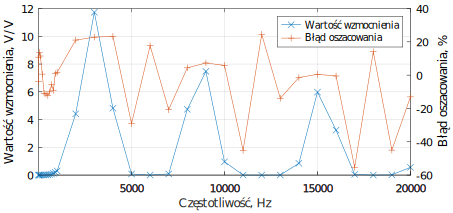
\includegraphics{obrazki/mono_freqcomp}
\makecaption{fig:mono_freqcomp}{Zależność względnego błędu oszacowania wartości niepewności~\qty{24}{\numTej} wielkości wyjściowej toru pomiarowego w funkcji częstotliwości sygnału (oś prawa) oraz zależność wartości wzmocnienia wynikającego z transmitancji analizowanej wielkości wyjściowej algorytmu w funkcji częstotliwości (oś lewa) dla przypadku o znanej wartości amplitudy sygnału ($c$)}
\end{center}
\end{figure}

Na podstawie uzyskanych wyników eksperymentu zauważyć można, że najistotniejsze właściwości analizowanego toru pomiarowego zostały zidentyfikowane poprawnie w przypadku, gdy tor ten przetwarza sygnały o częstotliwości powyżej~\qty{1}{kHz}. Dla sygnałów o niższej częstotliwości dominują źródła błędów, których parametry na etapie identyfikacji właściwości zastosowanego w eksperymencie źródła sygnału $s(t)$ wyznaczono niedokładnie, z uwagi na niedostateczne dane zawarte w dokumentacji tego urządzenia oraz brak pomiarowej weryfikacji tych właściwości. Dla pozostałych wielkości wyjściowych toru pomiarowego sformułować można wnioski zbieżne, jak te dotyczące analizowanej w przykładzie wielkości wyjściowej, przy czym wartości względnego błędu oszacowania wartości niepewności rozszerzonej dla kolejnych grup wielkości wyjściowych analizowanego toru pomiarowego zestawiono w tabeli~\ref{tab:pom_mono_meas_out}. Wyznaczone wartości średnie przedstawionych w tabeli~\ref{tab:pom_mono_meas_out} wielkości dotyczą średniej wyznaczonej dla wartości bezwzględnych przedstawionych wielkości dotyczących wybranej kolumny tabeli. Wyniki przeprowadzonego eksperymentu, wraz z wynikami uzyskanymi dla eksperymentu symulacyjnego, przeprowadzonego w poprzednim rozdziale, stanowią potwierdzenie zawartej we wstępie pracy tezy.

\DIFdelbegin %DIFDELCMD < \begin{table}[p]
%DIFDELCMD < \begin{center}
%DIFDELCMD < \makecaption{tab:pom_mono_meas_out}{Zestawienie uzyskanych na drodze eksperymentu pomiarowego wartości względnego błędu oszacowania wartości niepewności rozszerzonej dla kolejnych grup wielkości wyjściowych algorytmu dyskretnej transformacji falkowej wraz z zestawieniem średniej dla wartości bezwzględnych tej wielkości w przypadku sygnału monoharmonicznego}
%DIFDELCMD < \begin{tabular}[c]{| c *{6}{|S[table-format = +4.2]} |} \hline
%DIFDELCMD < \multirow{2}{*}{\textbf{$f_{s,o}$, Hz}} & \multicolumn{6}{c|}{\textbf{Zakres wielkości wyjściowych $X_{j}$ algorytmu}} \\ \cline{2-7}
%DIFDELCMD < & \text{$<0;3>$} & \text{$<4;7>$} & \text{$<8;15>$} & \text{$<16;31>$} & \text{$<32;63>$} & \text{$<64;127>$} \\ \hline
%DIFDELCMD < 100     &       -11.86  &       +5.19   &       -1.85   &       +10.75  &       -35.19  &       -16.81  \\ \hline
%DIFDELCMD < 200     &       +28.82  &       +6.93   &       -4.68   &       +14.92  &       -35.74  &       +9.16   \\ \hline
%DIFDELCMD < 300     &       -1.30   &       -7.80   &       -20.90  &       +2.02   &       -26.73  &       -24.13  \\ \hline
%DIFDELCMD < 400     &       +14.82  &       +9.72   &       -21.24  &       +6.57   &       -24.34  &       -8.11   \\ \hline
%DIFDELCMD < 500     &       +20.14  &       +3.47   &       -22.06  &       +7.05   &       -24.45  &       +2.60   \\ \hline
%DIFDELCMD < 600     &       +15.59  &       +5.26   &       -20.26  &       +1.90   &       -26.91  &       +2.63   \\ \hline
%DIFDELCMD < 700     &       +17.60  &       +4.32   &       -13.29  &       +1.89   &       -30.57  &       -2.79   \\ \hline
%DIFDELCMD < 800     &       +17.08  &       +4.60   &       -21.50  &       -5.32   &       -29.22  &       -23.74  \\ \hline
%DIFDELCMD < 900     &       +17.48  &       +11.34  &       -24.31  &       +0.85   &       -27.27  &       -1.63   \\ \hline
%DIFDELCMD < 1000    &       +8.21   &       +7.73   &       -25.74  &       -4.69   &       -25.40  &       +0.02   \\ \hline
%DIFDELCMD < 2000    &       +3.29   &       +2.64   &       +1.09   &       -20.46  &       -16.86  &       -7.01   \\ \hline
%DIFDELCMD < 3000    &       -3.79   &       -30.68  &       +4.90   &       -6.94   &       -13.90  &       -12.97  \\ \hline
%DIFDELCMD < 4000    &       +7.01   &       +6.83   &       +6.19   &       +5.93   &       -13.36  &       -12.55  \\ \hline
%DIFDELCMD < 5000    &       -3.89   &       -9.48   &       -34.86  &       -1.22   &       -16.32  &       -18.47  \\ \hline
%DIFDELCMD < 6000    &       -41.12  &       -44.26  &       -24.90  &       +2.17   &       -7.75   &       -11.18  \\ \hline
%DIFDELCMD < 7000    &       +3.23   &       +3.24   &       -42.26  &       +6.12   &       +4.16   &       -15.17  \\ \hline
%DIFDELCMD < 8000    &       -3.17   &       -2.91   &       -2.84   &       -2.92   &       -2.93   &       -13.20  \\ \hline
%DIFDELCMD < 9000    &       -11.64  &       -9.71   &       -0.23   &       -10.45  &       -1.02   &       -11.15  \\ \hline
%DIFDELCMD < 10000   &       +0.46   &       +2.65   &       +0.36   &       -36.93  &       +1.70   &       -6.30   \\ \hline
%DIFDELCMD < 11000   &       -5.20   &       -16.65  &       -51.18  &       -43.53  &       -2.96   &       -8.63   \\ \hline
%DIFDELCMD < 12000   &       -14.44  &       +12.91  &       -1.79   &       +8.32   &       -4.02   &       -9.30   \\ \hline
%DIFDELCMD < 13000   &       -1.97   &       -13.54  &       -30.63  &       -50.32  &       +1.64   &       -1.68   \\ \hline
%DIFDELCMD < 14000   &       -1.72   &       -3.37   &       -3.29   &       -28.87  &       -0.29   &       -0.07   \\ \hline
%DIFDELCMD < 15000   &       +2.91   &       +9.11   &       -0.91   &       -13.35  &       -0.47   &       +0.52   \\ \hline
%DIFDELCMD < 16000   &       -4.34   &       -5.18   &       -5.42   &       -6.05   &       -5.72   &       -5.28   \\ \hline
%DIFDELCMD < 17000   &       -0.28   &       -4.76   &       -54.00  &       -0.03   &       -5.31   &       +0.28   \\ \hline
%DIFDELCMD < 18000   &       -37.89  &       -40.72  &       -29.07  &       +2.83   &       -20.46  &       +2.19   \\ \hline
%DIFDELCMD < 19000   &       -4.67   &       -20.80  &       -48.50  &       -7.28   &       -46.33  &       -5.57   \\ \hline
%DIFDELCMD < 20000   &       -1.73   &       -7.82   &       -4.52   &       -4.44   &       -66.51  &       +5.45   \\ \hline
%DIFDELCMD < 21000   &       +3.68   &       +4.97   &       -0.77   &       -70.87  &       -69.58  &       +3.51   \\ \hline
%DIFDELCMD < Średnia &       10.31   &       10.62   &       17.45   &       12.83   &       19.57   &       8.07    \\ \hline
%DIFDELCMD < \end{tabular}
%DIFDELCMD < \end{center}
%DIFDELCMD < \end{table}
%DIFDELCMD < %%%
\DIFdelend \DIFaddbegin \begin{table}[p]
\begin{center}
\makecaption{tab:pom_mono_meas_out}{Zestawienie uzyskanych na drodze eksperymentu pomiarowego wartości względnego błędu oszacowania wartości niepewności rozszerzonej dla kolejnych grup wielkości wyjściowych algorytmu dyskretnej transformacji falkowej wraz z zestawieniem średniej dla wartości bezwzględnych tej wielkości w przypadku sygnału monoharmonicznego}
\begin{tabular}[c]{| c *{6}{|S[table-format = +4.2]} |} \hline
\multirow{2}{*}{\textbf{$f_{s,o}$, Hz}} & \multicolumn{6}{c|}{\textbf{Zakres wielkości wyjściowych $X_{j}$ algorytmu}} \\ \cline{2-7}
& $\interval{0}{3}$ & $\interval{4}{7}$ & $\interval{8}{15}$ & $\interval{16}{31}$ & $\interval{32}{63}$ & $\interval{64}{127}$ \\ \hline
100     &       -11.86  &       +5.19   &       -1.85   &       +10.75  &       -35.19  &       -16.81  \\ \hline
200     &       +28.82  &       +6.93   &       -4.68   &       +14.92  &       -35.74  &       +9.16   \\ \hline
300     &       -1.30   &       -7.80   &       -20.90  &       +2.02   &       -26.73  &       -24.13  \\ \hline
400     &       +14.82  &       +9.72   &       -21.24  &       +6.57   &       -24.34  &       -8.11   \\ \hline
500     &       +20.14  &       +3.47   &       -22.06  &       +7.05   &       -24.45  &       +2.60   \\ \hline
600     &       +15.59  &       +5.26   &       -20.26  &       +1.90   &       -26.91  &       +2.63   \\ \hline
700     &       +17.60  &       +4.32   &       -13.29  &       +1.89   &       -30.57  &       -2.79   \\ \hline
800     &       +17.08  &       +4.60   &       -21.50  &       -5.32   &       -29.22  &       -23.74  \\ \hline
900     &       +17.48  &       +11.34  &       -24.31  &       +0.85   &       -27.27  &       -1.63   \\ \hline
1000    &       +8.21   &       +7.73   &       -25.74  &       -4.69   &       -25.40  &       +0.02   \\ \hline
2000    &       +3.29   &       +2.64   &       +1.09   &       -20.46  &       -16.86  &       -7.01   \\ \hline
3000    &       -3.79   &       -30.68  &       +4.90   &       -6.94   &       -13.90  &       -12.97  \\ \hline
4000    &       +7.01   &       +6.83   &       +6.19   &       +5.93   &       -13.36  &       -12.55  \\ \hline
5000    &       -3.89   &       -9.48   &       -34.86  &       -1.22   &       -16.32  &       -18.47  \\ \hline
6000    &       -41.12  &       -44.26  &       -24.90  &       +2.17   &       -7.75   &       -11.18  \\ \hline
7000    &       +3.23   &       +3.24   &       -42.26  &       +6.12   &       +4.16   &       -15.17  \\ \hline
8000    &       -3.17   &       -2.91   &       -2.84   &       -2.92   &       -2.93   &       -13.20  \\ \hline
9000    &       -11.64  &       -9.71   &       -0.23   &       -10.45  &       -1.02   &       -11.15  \\ \hline
10000   &       +0.46   &       +2.65   &       +0.36   &       -36.93  &       +1.70   &       -6.30   \\ \hline
11000   &       -5.20   &       -16.65  &       -51.18  &       -43.53  &       -2.96   &       -8.63   \\ \hline
12000   &       -14.44  &       +12.91  &       -1.79   &       +8.32   &       -4.02   &       -9.30   \\ \hline
13000   &       -1.97   &       -13.54  &       -30.63  &       -50.32  &       +1.64   &       -1.68   \\ \hline
14000   &       -1.72   &       -3.37   &       -3.29   &       -28.87  &       -0.29   &       -0.07   \\ \hline
15000   &       +2.91   &       +9.11   &       -0.91   &       -13.35  &       -0.47   &       +0.52   \\ \hline
16000   &       -4.34   &       -5.18   &       -5.42   &       -6.05   &       -5.72   &       -5.28   \\ \hline
17000   &       -0.28   &       -4.76   &       -54.00  &       -0.03   &       -5.31   &       +0.28   \\ \hline
18000   &       -37.89  &       -40.72  &       -29.07  &       +2.83   &       -20.46  &       +2.19   \\ \hline
19000   &       -4.67   &       -20.80  &       -48.50  &       -7.28   &       -46.33  &       -5.57   \\ \hline
20000   &       -1.73   &       -7.82   &       -4.52   &       -4.44   &       -66.51  &       +5.45   \\ \hline
21000   &       +3.68   &       +4.97   &       -0.77   &       -70.87  &       -69.58  &       +3.51   \\ \hline
Średnia &       10.31   &       10.62   &       17.45   &       12.83   &       19.57   &       8.07    \\ \hline
\end{tabular}
\end{center}
\end{table}
\DIFaddend 

W przypadku, gdzie zakładano nieznane rzeczywiste wartości parametrów sygnału $s(t)$ ze względu na istniejące korelacje pomiędzy zdefiniowanymi składowymi sygnału błędu dynamicznego należało rozważyć dwie opcje, które dotyczyły kolejno dodatniej i ujemnej wartości błędu nastawy amplitudy. W takim przypadku oszacowana wartość niepewności związana z sygnałem błędu dynamicznego była również obarczona błędem wynikającym z niedokładnego oszacowania jednej ze składowych tego sygnału. Należy jednak zauważyć, że stosowanie wartości wielkości dla przypadku idealnego, podczas szacowania wartości parametru związanego z tą wielkością, nie wprowadza do obliczeń istotnych błędów. Wniosek ten znajduje swoje potwierdzenie między innymi w wynikach uzyskanych dla równań~\eqref{eq:pom_mono_unc_rand_ab} oraz~\eqref{eq:pom_mono_unc_rand_c}, a zatem założenia przyjęte w tej kwestii dla proponowanego w pracy modelu błędów są zasadne. Niemniej jednak, jeżeli znane są rzeczywiste wartości danego parametru, to należy wykorzystać je podczas obliczeń. Ze względu na fakt, że zastosowany w celu określania rzeczywistych wartości amplitudy oraz składowej stałej sygnału $s(t)$ multimetr Agilent 3458A cechuje bardzo duża dokładnością, w rozważaniach pominięto niepewność pomiaru tych wielkości.

Porównując wyniki zestawione w tabelach~\ref{tab:pom_mono_meas_in} oraz~\ref{tab:pom_mono_meas_out} zauważyć można, że mimo oszacowania wartości niepewności rozszerzonej wielkości wejściowej $x(i)$ algorytmu transformacji falkowej z błędem względnym na poziomie około~\qty{\pm 5}{\percent}, oszacowane wartości niepewności rozszerzonej na wyjściu algorytmu obarczone są znacznie większym błędem. Zjawisko to wynika z faktu, że analizowany algorytm wzmacnia sygnały błędów losowych, a zatem zwiększa się również składnik błędu związany z niedokładnością wyznaczenia parametrów tych sygnałów. W przypadku, gdy parametry dominującego źródła błędu zostały wyznaczone nieprawidłowo, oszacowana wartość niepewności rozszerzonej cechuje się dużą wartością względnego błędu oszacowania tej wielkości. Można zatem zauważyć, że dla przedstawionego toru pomiarowego najistotniejszym powodem rozbieżności pomiędzy oszacowanymi, a uzyskanymi pomiarowo wartościami niepewności rozszerzonych wielkości wyjściowych tego toru jest niedokładne oszacowanie parametrów sygnałów błędów losowych. Analogicznie, dla sytuacji w których parametry sygnałów błędów losowych byłyby wyznaczone poprawnie, natomiast parametry sygnałów błędów dynamicznych wyznaczone byłyby niedokładnie, spodziewać się można, że wartości względnego błędu oszacowania wartości niepewności rozszerzonej wielkości wyjściowych toru pomiarowego będą proporcjonalne do wartości wzmocnienia $|H_{i}(e^{j \omega_{s,o} T_{p}})|$ związanej z częstotliwością przetwarzanego sygnału $s(t)$.

\section{Przypadek sygnału poliharmonicznego}

Ostatni eksperyment weryfikujący poprawność założeń proponowanego w pracy modelu błędów oraz metody szacowania wypadkowej wartości niepewności rozszerzonych wielkości wyjściowych toru pomiarowego wykorzystującego algorytm dyskretnej transformacji falkowej dotyczy przypadku, gdy opisany w bieżącym rozdziale tor pomiarowy przetwarza sygnał trójkątny opisany w równaniach~\eqref{eq:pom_gen_triangle_ideal} oraz~\eqref{eq:pom_gen_triangle_real}. Podczas eksperymentu źródło napięcia wejściowego $s(t)$ stanowił generator przebiegów arbitralnych RIGOL~DG1011~\cite{rigol_fawg}, natomiast zadane parametry sygnału wejściowego wynosiły $\dot{E}_{s,o} = \qty{475}{mV}$ oraz $\dot{D}_{s,o} = \qty{500}{mV}$. Jako, że w poprzednim eksperymencie rozważono przypadek dotyczący nieznanych wartości rzeczywistych wartości parametrów amplitudy oraz składowej stałej, omawiany eksperyment zakłada znajomość tych parametrów. Na podstawie wyników pomiarów przeprowadzonych za pomocą multimetru Agilent 3458A przyjmuje się $\tilde{E}_{s,o} = \qty{479.65}{mV}$ oraz $\tilde{D}_{s,o} = \qty{505.85}{mV}$.

Zgodnie z założeniem~\eqref{eq:pom_gen_var_rand_saw} oraz równaniem~\eqref{eq:pom_varx_rand_prop} w analizowanym przypadku wariancję sygnału błędu losowego $e_{x,rp}(i)$, związanego z nieliniowością stosowanego źródła sygnału $s(t)$, opisać można równaniem:
\begin{equation}
\sigma_{x,rp}^{2} \cong \frac{\num{e-6}}{3} \emb{\tilde{E}_{s,o} + \tilde{D}_{s,o}}^{2} = \frac{\num{e-6}}{3} \DIFdelbegin %DIFDELCMD < \emb{\num{0.47970} + \num{0.50585}}%%%
\DIFdelend \DIFaddbegin \emb{\num{0.47965} + \num{0.50585}}\DIFaddend ^{2} = \qty{0.32}{\micro V} \label{eq:pom_multi_rand_var_in},
\end{equation}
przy czym zakłada się jednakowe prawdopodobieństwo realizacji każdej z wartości omawianego sygnału błędu, stąd przy założeniu liniowości analizowanego obiektu zachodzi $c_{x,rp} = c_{s,r} = c_{u}$. Należy zaznaczyć, że pomimo zmiany rodzaju rozkładu analizowanego sygnału błędu w stosunku do przypadku opisanego w poprzednim podrozdziale, treść równania~\eqref{eq:pom_mono_unc_rand_all} pozostaje niezmienna dla analizowanego przypadku, co wynika z treści równania~\eqref{eq:alg_outerr} oraz założeń centralnego twierdzenia granicznego.

Jako, że rzeczywista wartość parametru składowej stałej jest znana, a dodatkowo eksperyment przeprowadzany był w tych samych warunkach otoczenia, w jakich identyfikowano parametry przedstawionego toru pomiarowego, zakłada się, że sygnały  $e_{s,x}(t) = 0$ oraz $e_{x,sw}(i) = 0$. Wobec przyjętych założeń zachodzi zatem $U_{i,s} = \qty{0}{V}$. Podobne założenie przyjmuje się odnośnie sygnału błędu dynamicznego $e_{s,d}(t) = 0$, wynikającego z błędu nastawy amplitudy sygnału, a zatem zachodzi $e_{x,dp}(i) = 0$.

Najistotniejszą różnicę, w stosunku do poprzedniego eksperymentu, stanowi przebieg wypadkowego sygnału błędu dynamicznego $e_{x,d}(i) = e_{x,dw}(i)$ na wejściu algorytmu dyskretnej transformacji falkowej. W eksperymencie poprzednim sygnał ten składał się z jednej harmonicznej o pulsacji równej pulsacji sygnału $s(t)$, natomiast w bieżącym eksperymencie sygnał ten składa się z wielu harmonicznych. W dalszej części podrozdziału przyjmuje się, że analizowane będą wszystkie harmoniczne których pulsacja \DIFdelbegin \DIFdel{$\omega_{x,j} < \pi f_{p}$}\DIFdelend \DIFaddbegin \DIFadd{$\omega_{x,j} \le \pi f_{p}$}\DIFaddend . Zgodnie z definicją daną równaniem~\eqref{eq:pom_errx_dyn_self} każda harmoniczna sygnału błędu dynamicznego $e_{x,d}(i)$ złożona jest z dwóch składników. Wartość wariancji związanej z wybraną harmoniczną wyznaczana jest identycznie, jak przedstawiono w przykładzie opisanym równaniami~\eqref{eq:pom_mono_dyn_sum_param_amp_mid_val_c} oraz~\eqref{eq:pom_mono_dyn_unc_c}. Na podstawie wariancji kolejnych harmonicznych sygnału błędu dynamicznego wyznaczane są związane z nimi wartości niepewności rozszerzonej, zgodnie z równaiem~\eqref{eq:pom_uncout_dyn}.

Omawiany eksperyment pomiarowy przeprowadzono stosując metodologię identyczną, jak w przypadku poprzedniego eksperymentu. Wypadkową wartość niepewności rozszerzonej szacowano zgodnie z równaniem~\eqref{eq:pom_uncout_sum}, którego składniki wyznaczano zgodnie z równaniami od~\eqref{eq:pom_uncout_stat} do~\eqref{eq:pom_uncout_dyn}, natomiast wartość wypadkową wariancji szacowano zgodnie z zależnością~\eqref{eq:pom_varout_sum}. W przypadku uzyskanych realizacji sygnału błędu $e_{i,\Sigma}(j)$, zdefiniowanego w równaniu~\eqref{eq:alg_out_err}, wartość niepewności rozszerzonej wyznaczano zgodnie z równaniem~\eqref{eq:unc_summation}. Ze względu na fakt, że obliczenia wykonywane były w sposób identyczny, jak przedstawiano w pracy wielokrotnie dla omawianych wcześniej przykładów, w bieżącym rozdziale nie zostały one przedstawione, co wynika z liczby analizowanych harmonicznych sygnału błędu dynamicznego.

W tabeli~\ref{tab:pom_multi_meas_24} zestawiono wyniki przeprowadzonego eksperymentu dla wybranych wartości częstotliwości podstawowej harmonicznej sygnału $s(t)$, dotyczące~\qty{24}{\numTej} wielkości wyjściowej toru pomiarowego. Indeksem $c$ oznaczono wartości oszacowane na podstawie przyjętych założeń oraz proponowanej metody wyznaczania wypadkowej wartości niepewności rozszerzonej, natomiast indeksem $m$ oznaczono wartości uzyskane pomiarowo. Oznaczony symbolem $\delta_{c}$ błąd względny oszacowania wartości wypadkowej niepewności rozszerzonej wyznaczono zgodnie z równaniem~\eqref{eq:unc_error}.

\begin{table}[htb!]
\begin{center}
\makecaption{tab:pom_multi_meas_24}{Zestawienie wyników eksperymentu pomiarowego mającego na celu weryfikacje poprawności zastosowanych parametrów modelu błędów oraz skuteczności zaproponowanej metody wyznaczania wypadkowej niepewności rozszerzonej dla~\qty{24}{\numTej} wielkości wyjściowej algorytmu dyskretnej transformacji falkowej w przypadku sygnału poliharmonicznego}
\begin{tabular}[c]{| c *{4}{|S[table-format = 5.2]} *{2}{|S[table-format = 2.2]} | S[table-format = +3.2] |} \hline
\multirow{2}{*}{$f_{s,o}$} & \multicolumn{2}{c|}{\textbf{Wariancja, \micro V}} & \multicolumn{2}{c|}{\textbf{Niepewność, mV}} & \multicolumn{2}{c|}{\textbf{Kształt}} & \textbf{Błąd, \%} \\ \cline{2-8}
& $\sigma_{c}^{2}$ & $\sigma_{m}^{2}$ & $U_{c}$ & $U_{m}$ & $c_{c}$ & $c_{m}$ & $\delta_{c}$ \\ \hline
100     &       2.70    &       0.34    &       3.22    &       1.15    &       1.96    &       1.97    &       +181.14 \\ \hline
200     &       2.72    &       0.38    &       3.24    &       1.20    &       1.97    &       1.96    &       +169.91 \\ \hline
300     &       2.77    &       0.36    &       3.30    &       1.18    &       1.98    &       1.97    &       +180.28 \\ \hline
400     &       2.85    &       0.41    &       3.37    &       1.26    &       1.99    &       1.96    &       +167.87 \\ \hline
500     &       2.99    &       0.49    &       3.47    &       1.38    &       2.00    &       1.97    &       +150.70 \\ \hline
600     &       3.22    &       0.59    &       3.60    &       1.51    &       2.01    &       1.98    &       +137.92 \\ \hline
700     &       3.52    &       0.76    &       3.77    &       1.73    &       2.01    &       1.98    &       +118.18 \\ \hline
800     &       3.92    &       1.01    &       3.96    &       2.00    &       2.00    &       1.99    &       +98.06  \\ \hline
900     &       4.44    &       1.35    &       4.19    &       2.32    &       1.99    &       1.99    &       +80.95  \\ \hline
1000    &       5.07    &       2.23    &       4.45    &       2.83    &       1.98    &       1.90    &       +57.22  \\ \hline
2000    &       29.54   &       26.18   &       8.81    &       7.43    &       1.62    &       1.45    &       +18.60  \\ \hline
3000    &       12.52   &       10.29   &       6.30    &       5.06    &       1.78    &       1.58    &       +24.40  \\ \hline
4000    &       144.06  &       151.70  &       17.53   &       18.01   &       1.46    &       1.46    &       -2.69   \\ \hline
5000    &       858.17  &       946.18  &       41.80   &       42.74   &       1.43    &       1.39    &       -2.21   \\ \hline
\multicolumn{7}{|c|}{Średnia wartości bezwzględnych wielkości $\delta_{c}$}                             &       99.30   \\ \hline
\end{tabular}
\end{center}
\end{table}

Na podstawie danych zestawionych w tabeli~\ref{tab:pom_multi_meas_24} zauważyć można, że oszacowane wartości niepewności rozszerzonej dla analizowanej wielkości wyjściowej toru pomiarowego są znacznie większe, niż wartości uzyskane pomiarowo. Zważywszy na fakt, że wartość względnego błędu oszacowania wartości niepewności rozszerzonej maleje wraz ze wzrostem częstotliwości przetwarzanego sygnału, wnioskować można, że parametry związane z sygnałem błędu losowego $e_{s,r}(t)$, wynikającego z nieliniowości źródła sygnału $s(t)$, zostały oszacowane niepoprawnie. Omawiane parametry oszacowano na podstawie dokumentacji zastosowanego generatora, przy czym jedyną informację dotyczącą źródeł błędów dla sygnału trójkątnego stanowiła wartość błędu granicznego związanego z nieliniowością syntezowanego przebiegu. Można zatem przypuszczać, że rzeczywista wartość niepewności rozszerzonej, związanej z omawianym zjawiskiem, jest znacznie mniejsza, niż oszacowano.

Aby zweryfikować zasadność przedstawionej hipotezy obliczenia wykonano ponownie, dla założeń gdzie $e_{s,r}(t) = 0$, a zatem $U_{s,r} = \qty{0}{V}$. Podobnie, jak w przypadku synalu monoharmonicznego, obliczenia wykonano dla wszystkich grup wielkości wyjściowych toru pomiarowego. W tabeli~\ref{tab:pom_multi_meas_out} zestawiono wyznaczone wartości względnego błędu oszacowania wartości niepewności rozszerzonej dla kolejnych grup wielkości wyjściowych analizowanego toru pomiarowego oraz uśrednione wartości bezwzględne tych wielkości. Dane zawarte w tabeli~\ref{tab:pom_multi_meas_out} potwierdzają hipotezę postawioną w poprzednim akapicie. Zauważyć jednak można, że w wielu przypadkach oszacowana wartość wypadkowej niepewności rozszerzonej jest mniejsza, niż uzyskana pomiarowo. Oznacza to, że występują zjawiska zakłócające, których nie uwzględniono w analizie, przy czym ich rola jest istotna w procesie pomiaru.

\DIFdelbegin %DIFDELCMD < \begin{table}[htb!]
%DIFDELCMD < \begin{center}
%DIFDELCMD < \makecaption{tab:pom_multi_meas_out}{Zestawienie uzyskanych na drodze eksperymentu pomiarowego wartości względnego błędu oszacowania wartości niepewności rozszerzonej dla kolejnych grup wielkości wyjściowych algorytmu dyskretnej transformacji falkowej wraz z zestawieniem średniej dla wartości bezwzględnych tej wielkości w przypadku sygnału poliharmonicznego i założenia gdzie $e_{s,r}(t) = 0$}
%DIFDELCMD < \begin{tabular}[c]{| c *{6}{|S[table-format = +4.2]} |} \hline
%DIFDELCMD < \multirow{2}{*}{\textbf{$f_{s,o}$, Hz}} & \multicolumn{6}{c|}{\textbf{Zakres wielkości wyjściowych $X_{j}$ algorytmu}} \\ \cline{2-7}
%DIFDELCMD < & \text{$<0;3>$} & \text{$<4;7>$} & \text{$<8;15>$} & \text{$<16;31>$} & \text{$<32;63>$} & \text{$<64;127>$} \\ \hline
%DIFDELCMD < 100     &       -31.74  &       -18.30  &       -25.32  &       -9.30   &       -40.48  &       -34.87  \\ \hline
%DIFDELCMD < 200     &       -6.39   &       +2.14   &       -22.68  &       -10.27  &       -51.03  &       -23.34  \\ \hline
%DIFDELCMD < 300     &       +21.20  &       +20.64  &       -1.18   &       +1.08   &       -49.63  &       -18.57  \\ \hline
%DIFDELCMD < 400     &       +65.73  &       +29.27  &       -3.59   &       +5.50   &       -39.12  &       -22.97  \\ \hline
%DIFDELCMD < 500     &       +14.65  &       +40.25  &       +14.98  &       +9.67   &       -40.08  &       -16.96  \\ \hline
%DIFDELCMD < 600     &       +24.08  &       +37.64  &       +16.21  &       +17.20  &       -35.05  &       -18.27  \\ \hline
%DIFDELCMD < 700     &       +61.56  &       +28.17  &       +15.34  &       +20.33  &       -26.17  &       -16.41  \\ \hline
%DIFDELCMD < 800     &       +28.13  &       +13.22  &       +20.95  &       +19.36  &       -24.71  &       -11.50  \\ \hline
%DIFDELCMD < 900     &       +16.55  &       +20.13  &       +19.72  &       +18.25  &       -19.63  &       -9.93   \\ \hline
%DIFDELCMD < 1000    &       +9.33   &       +9.90   &       +22.41  &       +9.23   &       -16.38  &       -12.29  \\ \hline
%DIFDELCMD < 2000    &       -1.92   &       -3.09   &       -3.06   &       +5.52   &       -7.74   &       -31.03  \\ \hline
%DIFDELCMD < 3000    &       -41.35  &       -18.66  &       +33.60  &       -0.51   &       +2.48   &       -28.14  \\ \hline
%DIFDELCMD < 4000    &       -6.63   &       -4.28   &       -5.67   &       -6.04   &       +4.70   &       -30.49  \\ \hline
%DIFDELCMD < 5000    &       -18.69  &       -23.85  &       -15.71  &       -2.97   &       -14.34  &       -51.16  \\ \hline
%DIFDELCMD < Średnia &       24.85   &       19.25   &       15.74   &       9.66    &       26.54   &       23.28   \\ \hline
%DIFDELCMD < \end{tabular}
%DIFDELCMD < \end{center}
%DIFDELCMD < \end{table}
%DIFDELCMD < %%%
\DIFdelend \DIFaddbegin \begin{table}[htb!]
\begin{center}
\makecaption{tab:pom_multi_meas_out}{Zestawienie uzyskanych na drodze eksperymentu pomiarowego wartości względnego błędu oszacowania wartości niepewności rozszerzonej dla kolejnych grup wielkości wyjściowych algorytmu dyskretnej transformacji falkowej wraz z zestawieniem średniej dla wartości bezwzględnych tej wielkości w przypadku sygnału poliharmonicznego i założenia gdzie $e_{s,r}(t) = 0$}
\begin{tabular}[c]{| c *{6}{|S[table-format = +4.2]} |} \hline
\multirow{2}{*}{\textbf{$f_{s,o}$, Hz}} & \multicolumn{6}{c|}{\textbf{Zakres wielkości wyjściowych $X_{j}$ algorytmu}} \\ \cline{2-7}
& $\interval{0}{3}$ & $\interval{4}{7}$ & $\interval{8}{15}$ & $\interval{16}{31}$ & $\interval{32}{63}$ & $\interval{64}{127}$ \\ \hline
100     &       -31.74  &       -18.30  &       -25.32  &       -9.30   &       -40.48  &       -34.87  \\ \hline
200     &       -6.39   &       +2.14   &       -22.68  &       -10.27  &       -51.03  &       -23.34  \\ \hline
300     &       +21.20  &       +20.64  &       -1.18   &       +1.08   &       -49.63  &       -18.57  \\ \hline
400     &       +65.73  &       +29.27  &       -3.59   &       +5.50   &       -39.12  &       -22.97  \\ \hline
500     &       +14.65  &       +40.25  &       +14.98  &       +9.67   &       -40.08  &       -16.96  \\ \hline
600     &       +24.08  &       +37.64  &       +16.21  &       +17.20  &       -35.05  &       -18.27  \\ \hline
700     &       +61.56  &       +28.17  &       +15.34  &       +20.33  &       -26.17  &       -16.41  \\ \hline
800     &       +28.13  &       +13.22  &       +20.95  &       +19.36  &       -24.71  &       -11.50  \\ \hline
900     &       +16.55  &       +20.13  &       +19.72  &       +18.25  &       -19.63  &       -9.93   \\ \hline
1000    &       +9.33   &       +9.90   &       +22.41  &       +9.23   &       -16.38  &       -12.29  \\ \hline
2000    &       -1.92   &       -3.09   &       -3.06   &       +5.52   &       -7.74   &       -31.03  \\ \hline
3000    &       -41.35  &       -18.66  &       +33.60  &       -0.51   &       +2.48   &       -28.14  \\ \hline
4000    &       -6.63   &       -4.28   &       -5.67   &       -6.04   &       +4.70   &       -30.49  \\ \hline
5000    &       -18.69  &       -23.85  &       -15.71  &       -2.97   &       -14.34  &       -51.16  \\ \hline
Średnia &       24.85   &       19.25   &       15.74   &       9.66    &       26.54   &       23.28   \\ \hline
\end{tabular}
\end{center}
\end{table}
\DIFaddend 

Podobnie, jak w przypadku eksperymentu dotyczącego monoharmonicznego sygnału wejściowego, oszacowane wartości niepewności rozszerzonych są zbieżne z tymi uzyskanymi pomiarowo dla sytuacji, gdzie dominującym źródłem błędu jest sygnał błędu dynamicznego. Dla przypadków, gdzie dominujące źródło błędów stanowi sygnał błędu losowego, oszacowane wartości niepewności rozszerzonych są mniejsze od uzyskanych eksperymentalnie. Wobec powyższych zauważyć można, że w przetwarzanym sygnale $s(t)$ występuje sygnał błędu $e_{s,r}(t)$, który pominięto w analizie. Niepewność rozszerzona związana z sygnałem błędu $e_{s,r}(t)$ jest jednak znacznie mniejsza, niż wynika z równania~\eqref{eq:pom_multi_rand_var_in}, natomiast bez przeprowadzenia odpowiedniej procedury pomiarowej ustalenie jej wartości jest niemożliwe.

\section{Podsumowanie rozdziału}

Jak założono we wstępie do pracy, skuteczność przedstawionej metody analizy właściwości metrologicznych toru pomiarowego stosującego algorytm dyskretnej transformacji falkowej jest uwarunkowana dokładnością wyznaczenia parametrów modelu błędów tego toru. W rozdziale przedstawiono przykładowy tor pomiarowy oraz zaproponowano procedurę identyfikacji parametrów zaproponowanego w pracy modelu błędów tego toru, a dodatkowo wskazano w jaki sposób modelować można właściwości związane z przetwarzanym przez tor pomiarowy sygnałem wejściowym. Zaproponowany algorytm identyfikacji \DIFaddbegin \DIFadd{właściwości toru pomiarowego }\DIFaddend miał na celu określenie najważniejszych źródeł błędów oraz ich parametrów, przy czym zakładał on pozyskanie jak największej liczby informacji na podstawie dokumentacji stosowanych komponentów tego toru. W przypadku, gdy dokumentacja urządzenia nie zapewniała dostatecznych informacji na temat charakteru analizowanego źródła błędu, stosowano pomiarową metodę identyfikacji właściwości tego obiektu.

Do wyznaczenia właściwości statycznych przedstawionego toru pomiarowego zastosowano kalibrator FLUKE~5700A~\cite{fluke_manual}, a zatem zakładać można, że właściwości te zostały określone dokładnie. W przypadku właściwości dynamicznych, parametry modelu błędów oszacowano stosując opisaną procedurę pomiarową, której wyniki obarczone były wieloma źródłami błędów. Dodatkowo na podstawie uzyskanych wyników pomiarów przeprowadzono aproksymacje charakterystyki obiektu, a zatem wyznaczone parametry modelu błędów były niedokładne. Oszacowana wartość przesunięcia fazowego, wynikającego z niedoskonałych właściwości dynamicznych analizowanego toru pomiarowego, jest zawyżona dla harmonicznych przetwarzanego sygnału o niskich częstotliwościach (poniżej około~\qty{1}{kHz}).

Zastosowanie oscyloskopu w celu oszacowania wartości wzmocnienia statycznego wprowadza bardzo duży błąd oraz rozrzut uzyskiwanych wyników. Można jednak zauważyć, że w opisywanym przypadku toru pomiarowego wielkość ta została oszacowana poprawnie, a przyjęte uproszczenia nie miały znaczącego wpływu na uzyskiwane wartości niepewności rozszerzonych. Należy jednak \DIFdelbegin \DIFdel{zauważyć}\DIFdelend \DIFaddbegin \DIFadd{zaznaczyć}\DIFaddend , że w przypadkach, gdzie znajomość dokładnej wartości wzmocnienia w funkcji częstotliwości jest istotna, należy zastosować przyrząd pomiarowy umożliwiający jej wyznaczenie w sposób odpowiednio dokładny.

Mimo, że przyjęte odnośnie zastosowanego modelu błędów parametry pozwoliły na wyznaczenie niepewności wielkości wejściowych algorytmu dyskretnej transformacji falkowej z dokładnością około~\qty{\pm 5}{\percent}, co przedstawiono w tabeli~\ref{tab:pom_mono_meas_in}, względny błąd oszacowania wartości niepewności wielkości wyjściowych tego algorytmu jest znacznie większy. Sytuacja ta spowodowana jest faktem, że transmitancję związaną z pojedynczą wielkością wyjściową algorytmu dyskretnej transformacji falkowej traktować można jak aktywny filtr. Z uwagi na omawianą właściwość, dla analizowanej wielkości przenoszone są jedynie wybrane sygnały błędów ze względu na ich widmową gęstość mocy, co wynika z transmitancji analizowanej wielkości wyjściowej. Jako, że sygnały o wybranych częstotliwościach są wzmacniane, wzmacniany jest też błąd związany z oszacowaniem parametrów tych sygnałów.

Na podstawie przeprowadzonych eksperymentów zauważyć można, że główne źródło niedokładności oszacowania wartości niepewności rozszerzonych wielkości wyjściowych analizowanego \DIFaddbegin \DIFadd{toru pomiarowego }\DIFaddend stanowiło niedokładne wyznaczanie parametrów sygnałów błędów zawartych w przetwarzanym przez \DIFdelbegin \DIFdel{tor pomiarowy }\DIFdelend \DIFaddbegin \DIFadd{niego }\DIFaddend sygnale $s(t)$. Poza stosowaniem dodatkowego multimetru w celu określenia wartości amplitudy oraz składowej stałej sygnału $s(t)$ nie przeprowadzono żadnej procedury identyfikacji sygnałów błędów związanych ze stosowanym generatorem. Wszelkie informacje dotyczące możliwych zjawisk zakłócających proces syntezy napięcia wyjściowego czerpano z dokumentacji urządzenia, przy czym dane te były bardzo ogólne i odnosiły się do serii stosowanego modelu urządzenia. Należy zatem indywidualnie dla każdego urządzenia identyfikować jego właściwości, jeżeli istotne jest określenie dokładnych parametrów modelu błędów tego urządzenia.

Należy zauważyć, że celem przeprowadzonego eksperymentu było jedynie potwierdzenie zawartej w pracy tezy odnośnie wpływu dokładności wyznaczania parametrów modelu błędów na dokładność szacowania wartości wypadkowej niepewności rozszerzonej dla analizowanego toru pomiarowego. Analiza właściwości kolejnych fragmentów tego toru została przeprowadzona na potrzeby określenia omawianych parametrów i nie stanowiła bezpośrednio tematu pracy. \DIFaddbegin \DIFadd{Zasadność zaproponowanej metody szacowania wypadkowej wartości niepewności rozszerzonej oraz przedstawionego w pracy modelu błędu zostały potwierdzone w poprzednim rozdziale pracy.
}\DIFaddend 

\chapter{Podsumowanie pracy}

Zaproponowany w pracy model błędów umożliwia opis właściwości metrologicznych torów pomiarowych złożonych zarówno z części przetwarzania analogowego, jak i cyfrowego. Model ten obejmuje dwa rodzaje właściwości obiektu: dynamiczne -- związane z widmem przetwarzanego sygnału, oraz statyczne -- niezależne od widma przetwarzanego sygnału. Stosowanie zaproponowanego modelu błędów jest możliwe bez znajomości dokładnej struktury wewnętrznej analizowanego układu, a zatem model ten znajduje swoje zastosowanie do opisu między innymi urządzeń typu \enquote{SoC}. Parametry modelu błędów mogą być pozyskiwane na drodze eksperymentu pomiarowego, jak i szacowane na podstawie dokumentacji analizowanego urządzenia.

Opis właściwości metrologicznych analizowanego obiektu\DIFaddbegin \DIFadd{, }\DIFaddend wykorzystujący miarę wariancji sygnału błędu na wyjściu tego obiektu\DIFaddbegin \DIFadd{, }\DIFaddend jest znacznie bardziej przystępny z punktu widzenia skomplikowania obliczeń, niż opis wykorzystujący miarę niepewności rozszerzonej (w szczególności, gdy kolejne sygnały błędów nie są ze sobą w żaden sposób skorelowane). Opis ten nie dostarcza jednak informacji o prawdopodobieństwie uzyskania danej wartości realizacji sygnału błędu, a zatem jest mniej użyteczny, niż ten wykorzystujący miarę niepewności rozszerzonej.

Zastosowana w pracy metoda szacowania wypadkowej wartości niepewności rozszerzonej, wykorzystująca metodę redukcyjnej arytmetyki interwałowej, wraz z zaproponowaną modyfikacją zapewnia wyniki zbieżne z uzyskiwanymi metodą Monte-Carlo. Ze względu na niską złożoność obliczeniową omawianej metody, jej stosowanie jest możliwe w czasie rzeczywistym, również w przypadku zmiany parametrów modelu błędów lub widma przetwarzanego sygnału. Ograniczeniem przedstawionej metody jest konieczność wstępnego wyznaczenia wartości dla współczynników kształtu, przy czym procedura ta nie może odbywać się w czasie rzeczywistym, natomiast jest ona jednorazowa. W przypadku wystąpienia korelacji pomiędzy analizowanymi sygnałami błędów należy wyznaczyć wypadkowe wartości niepewności rozszerzonej dla skorelowanych grup sygnałów lub zastosować inną, niż zaproponowano w pracy, metodę wyznaczania wartości współczynników koherencji. Niezależnie, czy obliczenia prowadzone są z wykorzystaniem budżetu niepewności obejmującego wszystkie źródła błędów, czy stosowane są wypadkowe parametry dla wyróżnionych w pracy grup sygnałów błędów, omawiana metoda zapewnia bardzo zbliżone wyniki. Należy jednak zaznaczyć, że wyznaczanie wypadkowych wartości niepewności rozszerzonej w przypadku nietypowego kształtu rozkładu wypadkowego sygnału błędu uniemożliwia wykorzystanie wyznaczonej wartości niepewności rozszerzonej w dalszych obliczeniach. Właściwość ta spowodowana jest koniecznością znajomości wartości współczynników kształtu analizowanych par sygnałów. Jako, że wartości współczynników kształtu muszą zostać wyznaczone dla wcześniej zdefiniowanych parametrów rozkładu sygnałów, wyznaczenie wartości współczynników koherencji zgodnie z proponowaną w pracy metodą jest w omawianym przypadku niemożliwe. Należy zauważyć, że w praktyce wada ta jest nieistotna, \DIFdelbegin \DIFdel{ponieważ podczas implementacji algorytmu wykorzystującego przedstawioną metodę }\DIFdelend \DIFaddbegin \DIFadd{jeżeli podczas analizy }\DIFaddend stosowane są odpowiednio wyprowadzone zależności, wynikające z wzajemnych relacji \DIFaddbegin \DIFadd{zachodzących }\DIFaddend pomiędzy kolejnymi fragmentami toru pomiarowego\DIFdelbegin \DIFdel{, co wykazano w przedstawionych przykładach}\DIFdelend .

Przedstawienie algorytmu transformacji falkowej w postaci macierzowej umożliwia analizę właściwości metrologicznych tego algorytmu w sposób zbieżny z opisywaną w pracy metodą analizy cyfrowej cześć toru pomiarowego. Omawiany algorytm przedstawić można jako zbiór cyfrowych fragmentów toru pomiarowego, których model właściwości metrologicznych opisano w pracy. Wyznaczenie wartości współczynników macierzy transformacji dla analizowanego algorytmu odbywać się może analitycznie, na podstawie założeń dotyczących stosowanej rodziny falek, lub może zostać przeprowadzone na podstawie istniejącej implementacji tego algorytmu. Dla omawianej rodziny algorytmów istnieje również możliwość wyznaczenia wartości współczynników macierzy transformacji na podstawie transmitancji kolejnych wielkości wyjściowych algorytmu, a także przeprowadzenie operacji odwrotnej do opisanej. Jako, że w klasycznym przypadku wielkości wyjściowe algorytmu można podzielić na grupy\DIFdelbegin \DIFdel{o jednakowej transmitancji}\DIFdelend \DIFaddbegin \DIFadd{, w obrębie których transmitancja algorytmu jest identyczna}\DIFaddend , analiza może zostać uproszczona\DIFaddbegin \DIFadd{. Każda z omawianych grup wielkości wyjściowych związana jest z kolejną iteracją procesu dekompozycji sygnału}\DIFaddend .

Jak wykazały przeprowadzone eksperymenty, dokładność oszacowania wypadkowej wartości niepewności rozszerzonej wielkości wyjściowych analizowanego toru pomiarowego uwarunkowana jest głównie dokładnością wyznaczenia parametrów dla stosowanego modelu błędów. Z uwagi na fakt, że algorytmy transformacji falkowej stanowią zbiór filtrów, istotne jest prawidłowe oszacowanie parametrów najistotniejszych źródeł błędów dla każdej grupy sygnałów błędów: statycznych, dynamicznych oraz losowych. Nawet, jeżeli wielkości wejściowe algorytmu obarczone będą pewnym sygnałem błędu dominującego, to błąd ten może cechować się widmową gęstością mocy skoncentrowaną w okolicy częstotliwości, która dla wybranej wielkości wyjściowej jest tłumiona. W takim przypadku dla analizowanej wielkości wyjściowej przenoszone będą jedynie pozostałe sygnały błędów, przy czym sygnały te mogą być dodatkowo wzmacniane. Należy zatem zauważyć, że mimo niewielkiej rozbieżności w oszacowaniu wypadkowej wartości niepewności rozszerzonej wielkości wejściowych dla opisywanych algorytmów, wypadkowa wartość niepewności rozszerzonej na wyjściu tych algorytmów może być oszacowana niewłaściwie.

Przedstawione dotychczas wnioski podsumowujące zawarte w pracy rozważania potwierdzają założenia przedstawione we wstępie do pracy oraz sformułowaną w pracy tezę. Dalsze rozważania dotyczyć mogą uzupełniania przedstawionego modelu błędów o opis kolejnych zjawisk zakłócających proces pomiaru (np. wpływu opóźnień występujących w systemach pomiarowo-sterujących na wartości niepewności rozszerzonych wielkości analizowanych w tych systemach). Kolejne istotne zagadnie wymagające dalszych badań stanowi rozszerzenie opisanej w pracy metody wyznaczania wartości współczynników koherencji, obejmujące przypadki sygnałów skorelowanych, umożliwiające jednolite stosowanie omawianej metody w dowolnym przypadku.

Najważniejszy walor pracy stanowi przedstawienie jednolitego, spójnego modelu błędów umożliwiającego opis parametrów sygnałów błędów obecnych w torze pomiarowym. Zaproponowany model obejmuje etapy przetwarzania analogowego, cyfrowego oraz wskazuje wzajemne relacje pomiędzy omawianymi fragmentami. Sporządzone na potrzeby pracy podsumowanie najistotniejszych informacji dotyczących metrologicznych właściwości algorytmów transformacji falkowej umożliwia zastosowanie przedstawionego modelu błędu do opisu wpływu tych algorytmów na obecne w torze pomiarowym sygnały błędów. Istotną wartość pracy stanowi również zaproponowana metoda szacowania wypadkowej wartości niepewności rozszerzonej, przy czym metoda ta zapewnia wyniki zbliżone do tych uzyskiwanych metodą Monte-Carlo, oferując jednocześnie stosunkowo niewielką, w porównaniu do pozostałych obliczeń wykonywanych przez tor pomiarowy, złożoność obliczeniową również w przypadku zmiany wartości parametrów modelu błędów. Niniejsza praca stanowi zatem propozycję, w jaki sposób opisać można właściwości metrologiczne toru pomiarowego stosującego w swojej strukturze algorytm transformacji falkowej oraz w jaki sposób ilościowo określić niedokładność wyznaczania wartości wielkości wyjściowych tego toru. Oryginalność pracy podkreśla fakt, że dotychczas nie poruszano w literaturze problemu jednolitej analizy właściwości metrologicznych algorytmów dyskretnej transformacji falkowej.

\appendix
\end{document}
